\documentclass[paper=a4, 12pt, headings=standardclasses]{scrartcl}

\usepackage[utf8]{inputenc}
\usepackage[T1]{fontenc}
\usepackage[ngerman]{babel}
\usepackage{amsmath, amssymb}
\usepackage{siunitx}
\usepackage{graphicx}
\usepackage{wrapfig}
\usepackage[colorlinks, allcolors=black, urlcolor=blue]{hyperref}
%\usepackage{todonotes}
\usepackage[style=alphabetic]{biblatex}
\usepackage{pgf}
\usepackage{booktabs}
\usepackage[font=small, labelfont=bf]{caption}
\usepackage{setspace}
%\usepackage[left=44mm, right=44mm]{geometry}

\addbibresource{bibliography.bib}

\title{Integraler Quanten-Hall-Effekt}
\author{N. Galke \and M. J. Martins}
\date{}

\begin{document}
	\pagenumbering{gobble}

%\vspace*{0.3cm}
%\hrule
%\vspace{0.2cm}

\begin{center}

\Large
\textit{Versuchsauswertung}

\vspace{0.7cm}

\huge
\textbf{Untersuchung des Integralen Quanten-Hall-Effekts}

\vspace{1.1cm}

\Large
\textit{Laborpraktikum zur Vorlesung}

\vspace{0.2cm}

Einführung in die Festkörperphysik

%\vspace{0.5cm}
%\hrule

\vspace{2cm}

\Large
\textit{Leibniz Universität Hannover}\\
\vspace{0.5cm}
N. Galke \hspace{1cm} M. J. Martins

\end{center}

\normalsize

\vspace{1.4cm}

%\onehalfspacing
\section*{\centerline{Einleitung}}
\begin{addmargin}{3cm}
Der klassische Hall-Effekt ist bereits seit dem 19. Jahrhundert bekannt und (im klassischen Sinn) gut verstanden. Lew Landau vermutete jedoch schon kurz nach Begründung der Quantenmechanik, dass bei tiefen Temperaturen und hohen Magnetfeldern an geeigneten Systemen quantenmechanische Effekte beobachtet werden können, was spätestens durch Klaus von Klitzing 1980 auch experimentell nachgewiesen wurde.\\
Dieser \emph{Quanten-Hall-Effekt} soll in diesem Praktikum untersucht werden. Dazu werden einerseits einfache Magnetotransportmessungen durchgeführt (\ref{sec:Magnetotransport} \& \ref{sec:Mag_trans}) und andererseits weiterführende Messungen zu einem \glqq dauerhaften Photoeffekt\grqq\ (\ref{sec:Photoeffekt} \& \ref{sec:Photo}).
\end{addmargin}

\clearpage

\doublespacing
\tableofcontents

\clearpage

\pagenumbering{arabic}
\setcounter{page}{1}

\singlespacing


	\section{Theoretische Grundlagen}

\renewcommand{\V}[1]{\textbf{#1}}

\subsection{Klassischer Hall-Effekt}\label{sec:HallEffekt}

Bringt man einen stromführenden Leiter in ein äußeres Magnetfeld mit nicht zum Leiter paralleler Flussrichtung, so kann man senkrecht zur Stromrichtung eine Spannung (die \emph{Hall-Spannung}) messen. Dies bezeichnet man als \emph{Hall-Effekt}.
Dieser kann klassisch wie folgt erklärt werden:
Bewegen sich die Ladungsträger in einem Magnetfeld, das einen senkrechten Anteil zur Bewegungsrichtung hat, so wirkt auf die Ladungsträger (Ladung $q$, Geschwindigkeit $v$) eine nicht-verschwindende \emph{Lorentz-Kraft} senkrecht zum Strom und zum Magnetfeld (zumindest bei fehlenden äußeren elektrischen Feldern). Die dadurch hervorgerufene Ablenkung der Ladungsträger führt zur Ausbildung eines elektrischen Feldes, welches eine der ablenkenden Kraft entgegengerichtete Kraft erzeugt. Dieses \emph{Hall-Feld} baut sich solange auf, bis die daraus resultierende Kraft die des Magnetfeldes gerade kompensiert.
Es folgt die Bedingung an die Lorentz-Kraft
$$\V F_L = q(\V E_H + \V B\times \V v) = 0,$$
wobei $\V E_H$ das Hall-Feld bezeichne und $\V B$ senkrecht zum Strom sei.
Dadurch lassen sich die relevanten Größen in Beziehung setzen. Für die Hall-Spannung $U_H$ gilt bei einer Stromstärke $I$
\begin{equation}\label{eq:HallSpannung}
U_H\propto\frac{I\cdot B}{(\text{Probendicke}\parallel \V B)}.
\end{equation}
Die auftretende Proportionalitätskonstante wird \emph{Hall-Konstante} genannt und mit $A_H$ bezeichnet. Für diese gilt bei Leitung durch nur eine Sorte Ladungsträger
\begin{equation}
A_H = \frac{1}{nq}
\end{equation}
wobei $n$ die Ladungsträgerdichte (bzw. -konzentration) bezeichne. Diese kann also (bei
bekanntem $q$) durch Messung der Hall-Konstante bestimmt werden.
Anstatt $U_H$ lässt sich auch der \emph{Hall-Widerstand}
\begin{equation}\label{eq:HallWiderstand}
R_H = \frac{U_H}{I}
\end{equation}
betrachten, welcher zwar die Dimension eines Widerstands hat, jedoch nicht direkt mit einem „realen“ Widerstand identifiziert werden kann.\\
Gemessen werden jedoch stets $U_H$ und $I$.

\subsection{Zweidimensionales Elektronengas}
Um den \emph{Quanten-Hall-Effekt} beschreiben zu können, benötigt man das Modell des \emph{(2-dimensionalen) Elektronengases}\footnote{kurz: (2D)EG}.
Das EG ist ein Spezialfall des \emph{(idealen) Fermi-Gases}. Das ideale Fermi-Gas beschreibt passende Systeme durch ein Ensemble von nicht miteinander wechselwirkenden Fermionen in einem Potentialtopf, analog zum idealen Gas.
Angewandt auf die Elektronen im Festkörper bedeutet das also, dass neben den Wechselwirkungen der Elektronen miteinander auch das periodische Kristallpotential nicht wirklich berücksichtigt wird.\\

Dies kann aber zumindest teilweise durch das \emph{Bloch-Theorem} gerechtfertigt werden:\\
In einem periodischen Potential (endlicher Ausdehnung) erhält man eine Basis des Lösungsraumes bestehend aus Funktionen
$$\Psi_{\V k}(\V r) = u_{\V k}(\V r) e^{i\V k\cdot\V r},$$
wobei $\V k$ aus der ersten Brioullin-Zone stammt\footnote{Durch die Annahme endlicher Ausdehnung sind hier nur endlich viele $\V k$ möglich} und jedes $u_{\V k}$ dieselbe Periodizität wie das Potential hat.
Das periodische Potential der Kerne äußert sich also nur in einer Modulation\footnote{Störstellen können dieses Verhalten jedoch ändern} (\cite{czy15}, \cite{gro18}).\\

Speziell beim 2DEG nimmt man das Potential in einer Raumrichtung als Potentialtopf an. Für diese Richtung ergeben sich, wie für einen Potentialtopf üblich, (endlich viele) diskrete Energieniveaus. Die Menge der Lösungen der (stationären) eindimensionalen Schrödinger-Gleichung zu je einem dieser Energieeigenwerte bezeichnet man als \emph{Subband}.
In den anderen beiden Richtungen kann die Bewegung ungehindert ablaufen, wird also durch den Hamilton-Operator eines zweidimensionalen freien Teilchens beschrieben, jedoch mit einer effektiven Masse anstatt der üblichen Elektronenmasse.
Praktisch kann ein 2DEG z.B. an Grenzflächen passender Heterostrukturen erzeugt werden.

\subsection{Quanten-Hall-Effekt}\label{sec:Quanten-Hall-Effekt}
Führt man an einem 2DEG Versuche zum Hall-Effekt bei sehr niedrigen Temperaturen durch, so beobachtet man ein anderes Verhalten des Hall-Widerstands. Anstatt linear mit dem Magnetfeld anzuwachsen, bilden sich \emph{Hall-Plateaus} aus, die mit stärkerem Magnetfeld ausgeprägter werden. Beim Längswiderstand, also dem „realen“ Widerstand in Richtung des Stroms, kann man zudem die \emph{Shubnikov-de-Haas-Oszillationen} beobachten. Die Minima dieser Oszillation des Widerstands findet man bei denselben Feldstärken, wie die Hall-Plateaus. Für den Wert des Hall-Widerstands ergibt sich an diesen Stellen
\begin{equation}\label{eq:HallvKl}
R_H = \frac{1}{\nu}R_K
\end{equation}
wobei
\begin{equation}\label{eq:vKlitzing}
R_K := \frac{h}{e^2}
\end{equation}
als \emph{von-Klitzing-Konstante} bezeichnet wird und $\nu$ der sogenannte \emph{Füllfaktor} ist. Dieser nimmt zunächst ganzzahlige Werte an, die bei wachsenden Magentfeldern kleiner werden. Bei sehr hohen Magentfeldern erhält man jedoch auch echt rationale Werte für $\nu$. Man unterscheidet entsprechend den \emph{integralen} und den \emph{fraktionalen Quanten-Hall-
Effekt}.
Dem Füllfaktor lässt sich noch eine andere Bedeutung geben, welche auch die Namensgebung begründet.
In einem äußeren Magnetfeld wird die Bewegung der Elektronen auch in der „freien“ Ebene beeinflusst und entspricht dann nicht mehr der von freien Teilchen. Hat das Magnetfeld eine zur Ebene senkrechte Komponente, so lässt sich (klassisch) erklären, dass die Elektronen durch die Lorentz-Kraft auf Kreisbahnen gezwungen werden (vgl. \autoref{sc:HallEffekt}). Auf diesen bewegen sie sich mit der \emph{Zyklotronfrequenz}
$$\omega_C = \frac{eB}{m^*}$$
wobei das Magnetfeld $\V B$ wieder als senkrecht zur Ebene angenommen wurde und $m^*$ die effektive Masse bezeichne. Berechnet man nun die Energien, so erhält man neben den quantisierten Energien des Potentialtopfs und dem Beitrag der Spin-Magnetfeld-Wechselwirkung auch einen Beitrag durch Energieniveaus eines harmonischen Oszillators mit Frequenz $\omega_C$. Letztere werden auch als \emph{Landau-Niveaus} bezeichnet. Der Füllfaktor
lässt sich nun mit der Anzahl der besetzten Landau-Niveaus in Beziehung setzen. Man erhält dadurch letztlich
\begin{equation}\label{eq:Fuellfaktor}
\nu = \frac{n_eh}{Be}
\end{equation}
mit der Elektronenkonzentration $n_e$. Diese lässt sich also gemäß der Gleichung
\begin{equation}\label{eq:ElektrKonz1}
n_e = \frac{\nu Be}{h}
\end{equation}
aus einer Messung des Hall-Widerstands bestimmen, nachdem man die Plateaus den entsprechenden Füllfaktoren zugeordnet hat.
Alternativ kann man $U_H$, resp. $R_H$ auch gegen den Kehrwert $1/B$ des Magnetfeldes auftragen und die Periode
$\Delta$ bestimmen. $n_e$ ergibt sich dann gemäß
\begin{equation}\label{eq:ElektrKonz2}
n_e = \frac{2e}{h\Delta}.
\end{equation}
Für den klassischen Grenzfall $B\approx 0$ oder $T\gg0$ kann man (passend zu \eqref{eq:HallSpannung}-\eqref{eq:HallWiderstand}) auch
\begin{equation}\label{eq:ElektrKonz3}
n_e = \frac{1}{e}\left(\frac{\partial R_H}{\partial B}\right)^{-1}
\end{equation}
verwenden.\\
Die Elektronenmobilität ergibt sich zu
\begin{equation}\label{eq:Mobilitaet}
\mu_e \propto \frac{1}{e n_eR_{xx}(0)},
\end{equation}
wobei der Proportionalitätsfaktor durch das Verhältnis aus Kontaktabstand und Breite der Hallgeometrie gegeben ist.
\nocite{qhe}
\nocite{wiki-fg}
\nocite{wiki-he}

	\clearpage
	\section{Aufbau und Durchführung}
Der erste Schritt bestand darin, das Programm zu schreiben, welches den Messvorgang steuert, also Magnetfeld hoch- und runterfährt, sowie Messwerte ausliest und in einer Datei speichert. Dazu wurde LabView verwendet.

\subsection{Magnetotransportmessung}\label{sec:Magnetotransport}
Bei diesen Messungen geht es darum, die Magnetotransporteigenschaften der Probe zu bestimmen.

\begin{wrapfigure}[13]{r}{7.5cm}

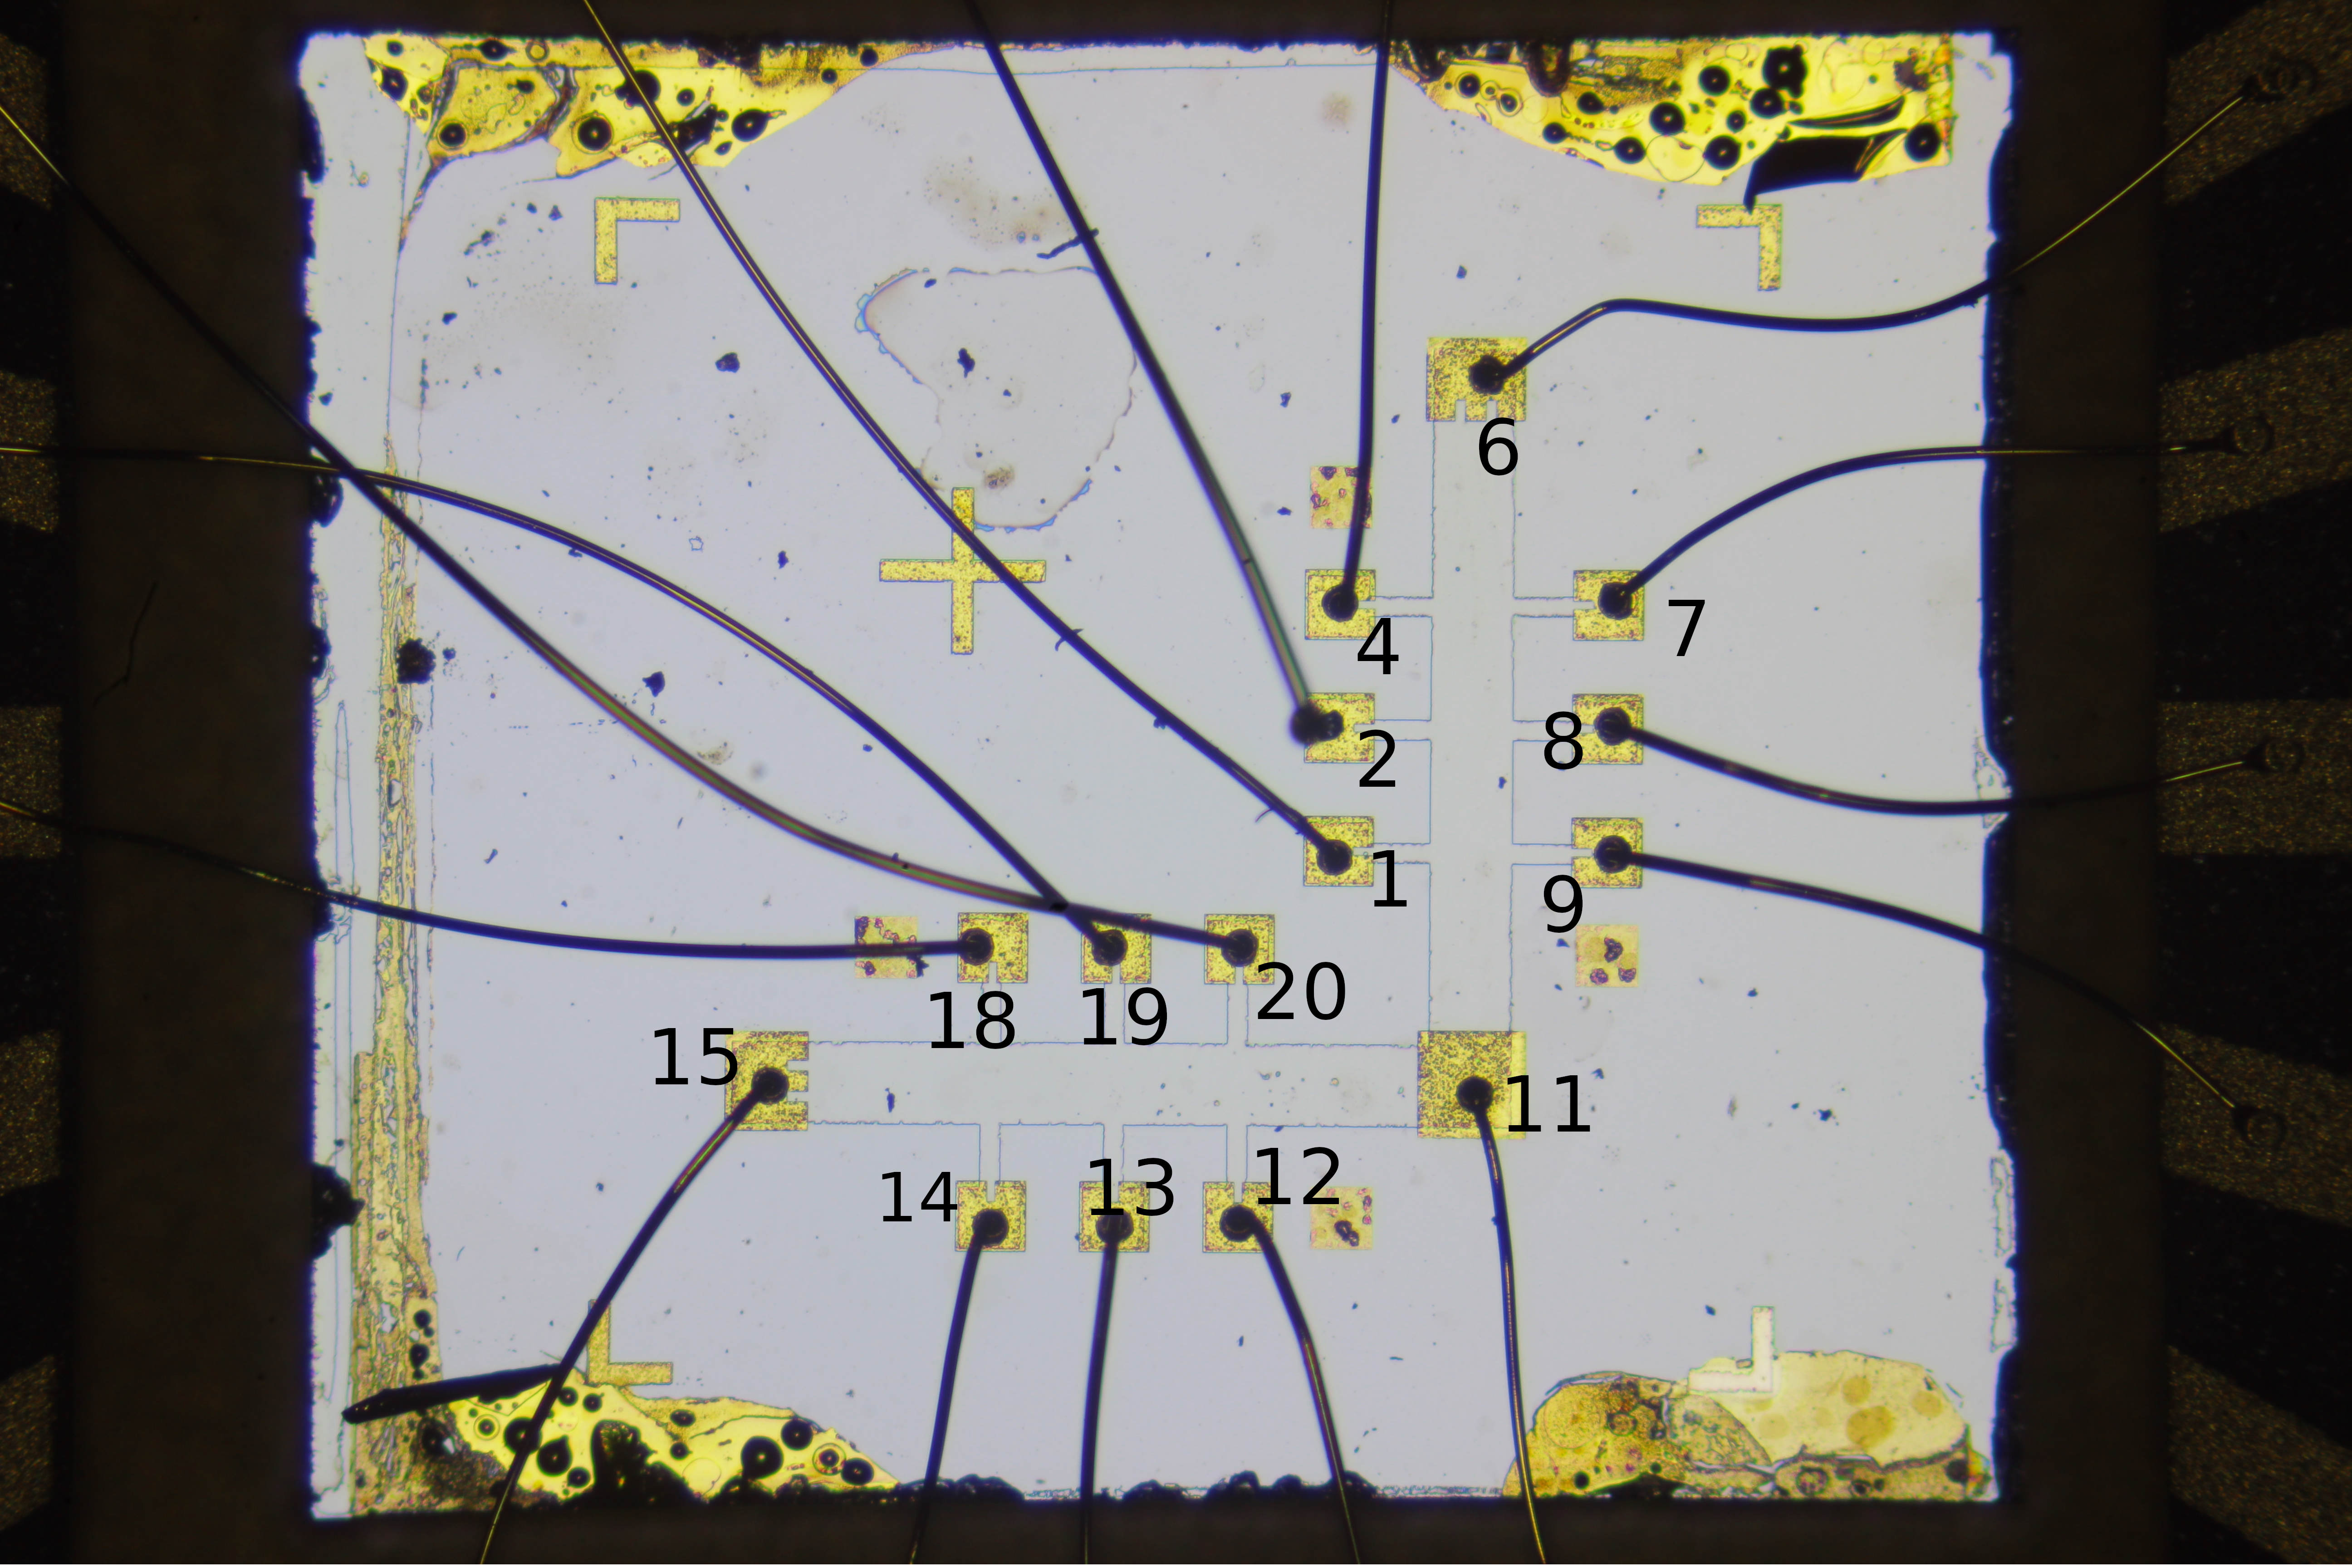
\includegraphics[scale=0.04]{Pictures/P07BondSchema.jpg}
\caption{Bond-Schema von Probe \emph{P07}}

\label{fig:P07}

\end{wrapfigure}
\hfill\\
Der Magnetprobenstab, an dessen unteren Ende sich eine Spule befindet, wird in der Heliumkanne platziert.
Die Probe (\emph{P07}, Bond-Schema siehe \autoref{fig:P07}) wird in den Probenstab eingesetzt und dieser wiederum in den Magnetprobenstab eingelassen.
Vor der ersten Messung muss lange genug gewartet werden, sodass die eingebrachten Bauteile abkühlen können.\\
Über ein Schaltbrett, das es erlaubt, auf die verschiedenen Kontakte der Hallgeometrie zuzugreifen, wird der Stab mit einer Stromquelle (\emph{Keithley 2400}) verbunden.
Zum Aufbauen des Magnetfelds wird ein weiteres Netzteil benötigt.
Mittels zweier \emph{Keithley 2000} werden Längs- und Querspannung gemessen.\\\\
Dabei wird der Längsstrom von $10\ \si{\micro A}$ an zwei verschiedene Kontaktpaare angelegt.
Für jedes Kontaktpaar werden die Spannungsmessgeräte wiederum mit jeweils zwei Kontaktpaaren verbunden, sodass vier Messreihen entstehen.
In jeder Messreihe wird das Magnetfeld von $0\ \si{T}$ auf $4\ \si{T}$ hochgefahren (oder andersherum) und in geeigneten Abständen werden Längs- und Querspannung aufgenommen.
Die Kontaktpaare sollen nach Möglichkeit verschieden sein, was jedoch aufgrund defekter Kontakte nicht immer uneingeschränkt möglich war.\\
Aus den Messwerten werden dann Elektronenkonzentration und -beweglichkeit bestimmt.\\\\
Die verwendeten Paarungen (inklusive den in \autoref{sec:Auswertung} verwendeten Bezeichnungen der Messreihen) sind in \autoref{tab:PairsP07} zu finden.\\

\begin{table}[ht]
\caption{Für die Messungen zum Magnetotransport verwendete Kontaktpaarungen}
\label{tab:PairsP07}
\centering
\begin{tabular}{cccc}
\toprule
Bezeichnung & Strom & Längswiderstand & Hallwiderstand\\
\midrule
P07\_1\_A & $6\rightarrow 11$ & $7\rightarrow 8$ & $1\rightarrow 9$\\
P07\_1\_B & $6\rightarrow 11$ & $7\rightarrow 9$ & $1\rightarrow 9$\\
P07\_2\_A & $11\rightarrow 15$ & $12\rightarrow 13$ & $20\rightarrow 12$\\
P07\_2\_B & $11\rightarrow 15$ & $20\rightarrow 18$ & $19\rightarrow 13$\\
\bottomrule
\end{tabular}
\end{table}
\subsection{Dauerhafter Photoeffekt}\label{sec:Photoeffekt}
Bei sehr tiefen Temperaturen kann der durch den Photoeffekt erzeugte Strom auch nach Ausschalten der Beleuchtung noch gemessen können.
Dies soll anhand dieser Messungen verifiziert werden.

\begin{wrapfigure}[13]{r}{7.5cm}
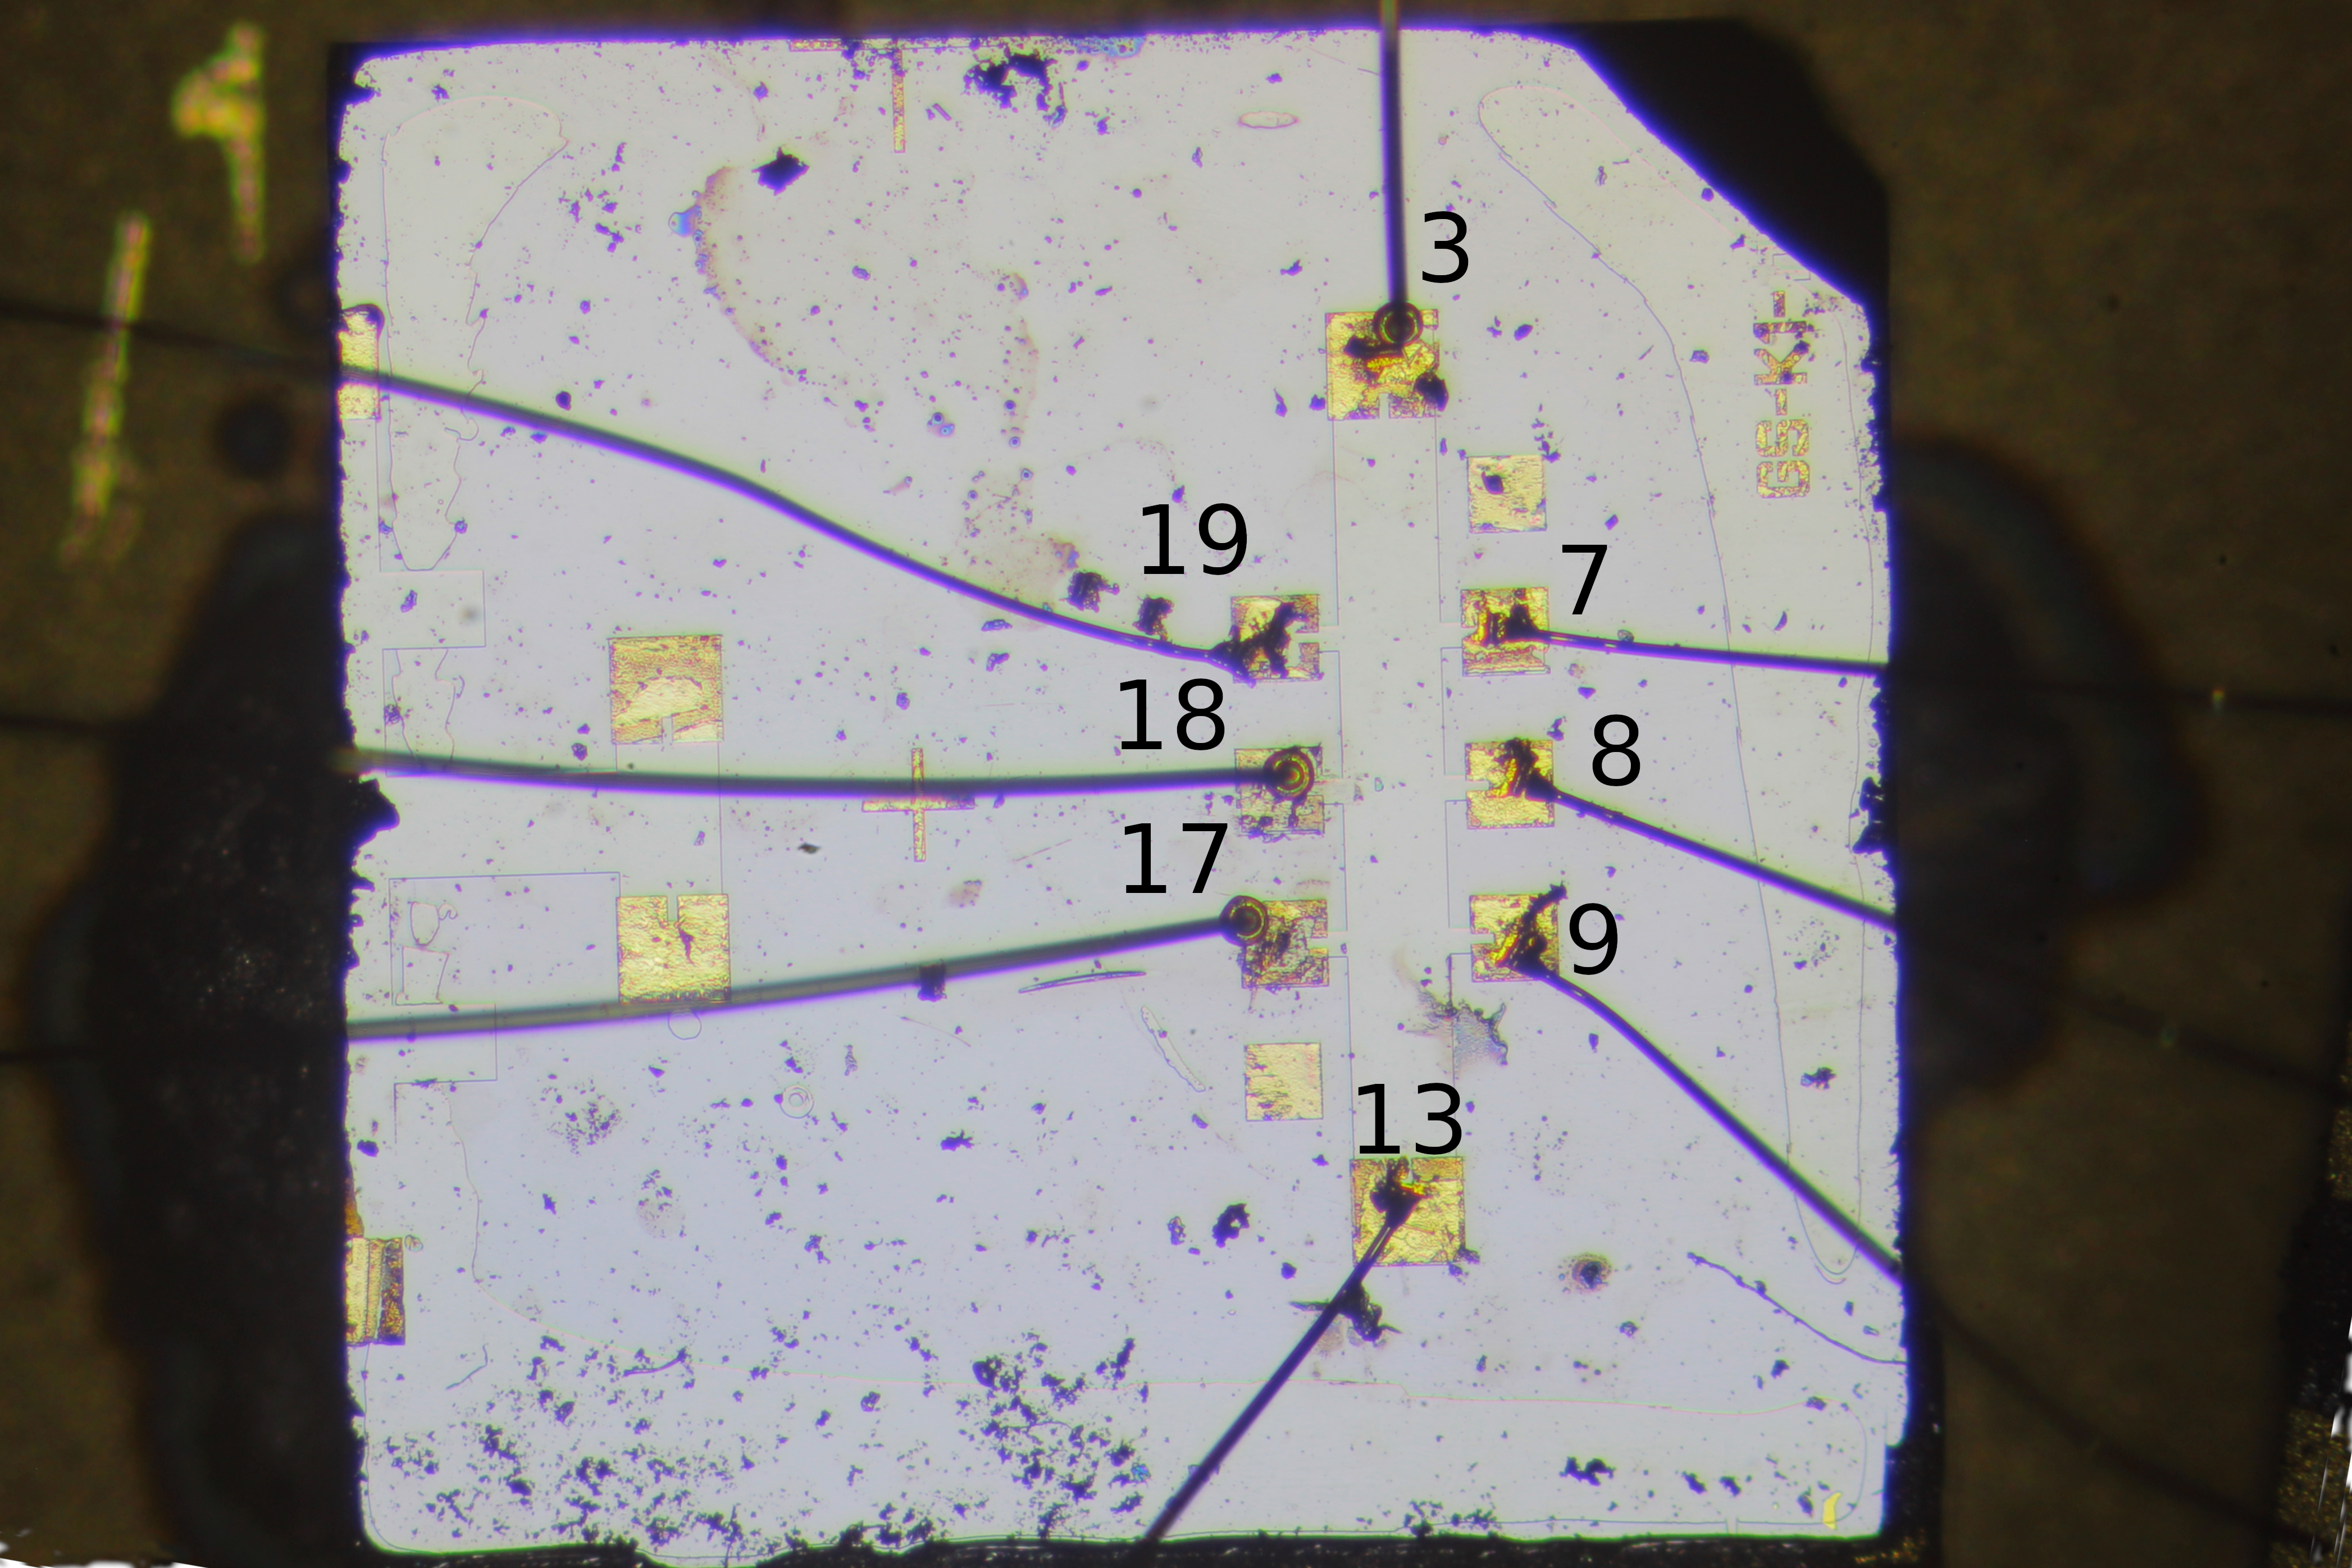
\includegraphics[scale=0.05]{Pictures/P04BondSchema}
\caption{Bond-Schema von Probe \emph{P04}}
\label{fig:P04}
\end{wrapfigure}
\hfill\\
Der Aufbau der Messung ist zum größten Teil identisch zu dem in \autoref{sec:Magnetotransport} beschriebenen. Es wird jedoch eine andere Probe (\emph{P04}, Bond-Schema siehe \autoref{fig:P04}) verwendet, auf welcher außerdem eine LED angebracht wird.

Bei diesen Messungen wird der Strom stets an dieselben Kontakte angelegt.
Zunächst werden für zwei Kombinationen von Kontakten Messungen analog zu \autoref{sec:Magnetotransport} durchgeführt. Die verwendeten Paarungen sind \autoref{tab:PairsP04} zu entnehmen.\\
Anschließend wird mit einem \emph{Keithley 2400} an die LED ein Strom von $8\ \si{mA}$ angelegt und die Probe für $60$ Sekunden beleuchtet.
Nach einer Wartezeit von zehn Minuten wird die Messung wiederholt.\\
Elektronenkonzentration und -beweglichkeit werden berechnet und verglichen.

\begin{table}[ht]
\caption{Für die Messungen zum Magnetotransport verwendete Kontaktpaarungen}
\label{tab:PairsP04}
\centering
\begin{tabular}{cccc}
\toprule
Bezeichnung & Strom & Längswiderstand & Hallwiderstand\\
\midrule
P04\_1 & $3\rightarrow 13$ & $7\rightarrow 8$ & $19\rightarrow 7$\\
P04\_2 & $3\rightarrow 13$ & $19\rightarrow 17$ & $17\rightarrow 9$\\
\bottomrule
\end{tabular}
\end{table}

	\clearpage

    	\section{Auswertung}

Zunächst einige Worte zu den mit LabView aufgenommenen Messwerten: da die Abtastrate der Messgeräte höher gewählt war als die Rate, mit der das Magnetfeld erhöht wurde, kam es vor, dass für gleiche Werte des Magnetfelds mehrere Messwerte aufgenommen wurden.

Zwischen diesen Werten mit konstantem Magnetfeld kann es in den gemessenen Spannungen / Widerständen natürlich zu Fluktuationen gekommen sein. Um einem Wert des Magnetfeld eindeutige Messwerte zuordnen zu können und zu verhindern, dass Messwerte doppelt auftreten (was zum Beispiel beim Fitten für eine ungerechtfertige Gewichtung gesorgt hätte), wurde daher über alle diese Werte gemittelt.

\subsection{Magnetotransportmessung}\label{sec:Mag_trans}
Die Vermessung des Magnetotransport wurde wie bereits in \autoref{sec:Magnetotransport} ausgeführt an Probe P07 und über 4 verschiedene Kontaktpaare für den Hallwiderstand / -spannung bzw. der für den Strom angelegten Spannung / dem dort beobachteten Widerstand durchgeführt. Aus diesen Werten lässt sich dann mit den in \autoref{sec:Quanten-Hall-Effekt} erläuterten Gleichungen auf drei unterschiedlichen Wegen die Elektronenkonzentration und die Ladungsträgermobilität bestimmen. 

Während jede dieser Methoden auf alle 4 Messreihen angewendet wurden, werden im Folgenden nur Darstellungen für eine repräsentativ angeführt. Die Vorgehensweisen lassen sich auf die Übrigen Reihen ohne nennenswerten Anpassungen übertragen - auf Unterschiede wird eingegangen. Die so bestimmten Größen werden für alle Messreihen angegeben und (vergleiched) diskutiert.

\subsubsection{Methode 1: Bestimmung der Hallplateaus}
Nach Gl. \ref{eq:ElektrKonz1} lässt sich aus der Lage der Hallplateaus sowie den entsprechenden Füllfaktoren die Elektronenkonzentration berechnet werden. Dafür muss nach Gl. \ref{eq:Fuellfaktor} der Füllfaktor bestimmt werden - wir benötigen daher zusätzlich die zu den Plateaus korrespondierenden Hallwiderstände.  Betrachten wir daher die repräsentative Darstellung einer Messreihe in Abb. \ref{abb:P07_Meth_1}:

Man erkennt sehr gut die SdH-Oszillation sowie zwei klare Hallplateaus für Magnetfelder mit $B>\SI{2}{\tesla}$. Auch für schwächere Magnetfelder lassen sich Hallplateaus ausmachen - allerdings deutlich weniger sicher. Für Magnetfelder $B<\SI{1}{\tesla}$ lassen sich keine Plateaus mehr erkennen. Die SdH-Oszillationen sind hingegen über einen deutlich größeren Wertebereich klar und ist mit eindeutigen Minima versehen. Wir haben uns daher entschieden, die zu Plataeus korrespondierenden Magnetfeldstärken (und damit dazu gehörige Hallwiderstände) aus den Minima der Oszillation zu bestimmen.

\begin{figure}[h!]
	\centering
	%% Creator: Matplotlib, PGF backend
%%
%% To include the figure in your LaTeX document, write
%%   \input{<filename>.pgf}
%%
%% Make sure the required packages are loaded in your preamble
%%   \usepackage{pgf}
%%
%% Figures using additional raster images can only be included by \input if
%% they are in the same directory as the main LaTeX file. For loading figures
%% from other directories you can use the `import` package
%%   \usepackage{import}
%% and then include the figures with
%%   \import{<path to file>}{<filename>.pgf}
%%
%% Matplotlib used the following preamble
%%   \usepackage[utf8x]{inputenc}
%%   \usepackage[T1]{fontenc}
%%
\begingroup%
\makeatletter%
\begin{pgfpicture}%
\pgfpathrectangle{\pgfpointorigin}{\pgfqpoint{6.012886in}{3.716168in}}%
\pgfusepath{use as bounding box, clip}%
\begin{pgfscope}%
\pgfsetbuttcap%
\pgfsetmiterjoin%
\definecolor{currentfill}{rgb}{1.000000,1.000000,1.000000}%
\pgfsetfillcolor{currentfill}%
\pgfsetlinewidth{0.000000pt}%
\definecolor{currentstroke}{rgb}{1.000000,1.000000,1.000000}%
\pgfsetstrokecolor{currentstroke}%
\pgfsetdash{}{0pt}%
\pgfpathmoveto{\pgfqpoint{0.000000in}{0.000000in}}%
\pgfpathlineto{\pgfqpoint{6.012886in}{0.000000in}}%
\pgfpathlineto{\pgfqpoint{6.012886in}{3.716168in}}%
\pgfpathlineto{\pgfqpoint{0.000000in}{3.716168in}}%
\pgfpathclose%
\pgfusepath{fill}%
\end{pgfscope}%
\begin{pgfscope}%
\pgfsetbuttcap%
\pgfsetmiterjoin%
\definecolor{currentfill}{rgb}{1.000000,1.000000,1.000000}%
\pgfsetfillcolor{currentfill}%
\pgfsetlinewidth{0.000000pt}%
\definecolor{currentstroke}{rgb}{0.000000,0.000000,0.000000}%
\pgfsetstrokecolor{currentstroke}%
\pgfsetstrokeopacity{0.000000}%
\pgfsetdash{}{0pt}%
\pgfpathmoveto{\pgfqpoint{0.592318in}{0.451986in}}%
\pgfpathlineto{\pgfqpoint{5.481911in}{0.451986in}}%
\pgfpathlineto{\pgfqpoint{5.481911in}{3.591168in}}%
\pgfpathlineto{\pgfqpoint{0.592318in}{3.591168in}}%
\pgfpathclose%
\pgfusepath{fill}%
\end{pgfscope}%
\begin{pgfscope}%
\pgfpathrectangle{\pgfqpoint{0.592318in}{0.451986in}}{\pgfqpoint{4.889593in}{3.139182in}}%
\pgfusepath{clip}%
\pgfsetbuttcap%
\pgfsetroundjoin%
\pgfsetlinewidth{0.501875pt}%
\definecolor{currentstroke}{rgb}{0.690196,0.690196,0.690196}%
\pgfsetstrokecolor{currentstroke}%
\pgfsetdash{{1.850000pt}{0.800000pt}}{0.000000pt}%
\pgfpathmoveto{\pgfqpoint{0.814572in}{0.451986in}}%
\pgfpathlineto{\pgfqpoint{0.814572in}{3.591168in}}%
\pgfusepath{stroke}%
\end{pgfscope}%
\begin{pgfscope}%
\pgfsetbuttcap%
\pgfsetroundjoin%
\definecolor{currentfill}{rgb}{0.000000,0.000000,0.000000}%
\pgfsetfillcolor{currentfill}%
\pgfsetlinewidth{0.803000pt}%
\definecolor{currentstroke}{rgb}{0.000000,0.000000,0.000000}%
\pgfsetstrokecolor{currentstroke}%
\pgfsetdash{}{0pt}%
\pgfsys@defobject{currentmarker}{\pgfqpoint{0.000000in}{-0.048611in}}{\pgfqpoint{0.000000in}{0.000000in}}{%
\pgfpathmoveto{\pgfqpoint{0.000000in}{0.000000in}}%
\pgfpathlineto{\pgfqpoint{0.000000in}{-0.048611in}}%
\pgfusepath{stroke,fill}%
}%
\begin{pgfscope}%
\pgfsys@transformshift{0.814572in}{0.451986in}%
\pgfsys@useobject{currentmarker}{}%
\end{pgfscope}%
\end{pgfscope}%
\begin{pgfscope}%
\definecolor{textcolor}{rgb}{0.000000,0.000000,0.000000}%
\pgfsetstrokecolor{textcolor}%
\pgfsetfillcolor{textcolor}%
\pgftext[x=0.814572in,y=0.354764in,,top]{\color{textcolor}\rmfamily\fontsize{8.000000}{9.600000}\selectfont \(\displaystyle 0.0\)}%
\end{pgfscope}%
\begin{pgfscope}%
\pgfpathrectangle{\pgfqpoint{0.592318in}{0.451986in}}{\pgfqpoint{4.889593in}{3.139182in}}%
\pgfusepath{clip}%
\pgfsetbuttcap%
\pgfsetroundjoin%
\pgfsetlinewidth{0.501875pt}%
\definecolor{currentstroke}{rgb}{0.690196,0.690196,0.690196}%
\pgfsetstrokecolor{currentstroke}%
\pgfsetdash{{1.850000pt}{0.800000pt}}{0.000000pt}%
\pgfpathmoveto{\pgfqpoint{1.370347in}{0.451986in}}%
\pgfpathlineto{\pgfqpoint{1.370347in}{3.591168in}}%
\pgfusepath{stroke}%
\end{pgfscope}%
\begin{pgfscope}%
\pgfsetbuttcap%
\pgfsetroundjoin%
\definecolor{currentfill}{rgb}{0.000000,0.000000,0.000000}%
\pgfsetfillcolor{currentfill}%
\pgfsetlinewidth{0.803000pt}%
\definecolor{currentstroke}{rgb}{0.000000,0.000000,0.000000}%
\pgfsetstrokecolor{currentstroke}%
\pgfsetdash{}{0pt}%
\pgfsys@defobject{currentmarker}{\pgfqpoint{0.000000in}{-0.048611in}}{\pgfqpoint{0.000000in}{0.000000in}}{%
\pgfpathmoveto{\pgfqpoint{0.000000in}{0.000000in}}%
\pgfpathlineto{\pgfqpoint{0.000000in}{-0.048611in}}%
\pgfusepath{stroke,fill}%
}%
\begin{pgfscope}%
\pgfsys@transformshift{1.370347in}{0.451986in}%
\pgfsys@useobject{currentmarker}{}%
\end{pgfscope}%
\end{pgfscope}%
\begin{pgfscope}%
\definecolor{textcolor}{rgb}{0.000000,0.000000,0.000000}%
\pgfsetstrokecolor{textcolor}%
\pgfsetfillcolor{textcolor}%
\pgftext[x=1.370347in,y=0.354764in,,top]{\color{textcolor}\rmfamily\fontsize{8.000000}{9.600000}\selectfont \(\displaystyle 0.5\)}%
\end{pgfscope}%
\begin{pgfscope}%
\pgfpathrectangle{\pgfqpoint{0.592318in}{0.451986in}}{\pgfqpoint{4.889593in}{3.139182in}}%
\pgfusepath{clip}%
\pgfsetbuttcap%
\pgfsetroundjoin%
\pgfsetlinewidth{0.501875pt}%
\definecolor{currentstroke}{rgb}{0.690196,0.690196,0.690196}%
\pgfsetstrokecolor{currentstroke}%
\pgfsetdash{{1.850000pt}{0.800000pt}}{0.000000pt}%
\pgfpathmoveto{\pgfqpoint{1.926121in}{0.451986in}}%
\pgfpathlineto{\pgfqpoint{1.926121in}{3.591168in}}%
\pgfusepath{stroke}%
\end{pgfscope}%
\begin{pgfscope}%
\pgfsetbuttcap%
\pgfsetroundjoin%
\definecolor{currentfill}{rgb}{0.000000,0.000000,0.000000}%
\pgfsetfillcolor{currentfill}%
\pgfsetlinewidth{0.803000pt}%
\definecolor{currentstroke}{rgb}{0.000000,0.000000,0.000000}%
\pgfsetstrokecolor{currentstroke}%
\pgfsetdash{}{0pt}%
\pgfsys@defobject{currentmarker}{\pgfqpoint{0.000000in}{-0.048611in}}{\pgfqpoint{0.000000in}{0.000000in}}{%
\pgfpathmoveto{\pgfqpoint{0.000000in}{0.000000in}}%
\pgfpathlineto{\pgfqpoint{0.000000in}{-0.048611in}}%
\pgfusepath{stroke,fill}%
}%
\begin{pgfscope}%
\pgfsys@transformshift{1.926121in}{0.451986in}%
\pgfsys@useobject{currentmarker}{}%
\end{pgfscope}%
\end{pgfscope}%
\begin{pgfscope}%
\definecolor{textcolor}{rgb}{0.000000,0.000000,0.000000}%
\pgfsetstrokecolor{textcolor}%
\pgfsetfillcolor{textcolor}%
\pgftext[x=1.926121in,y=0.354764in,,top]{\color{textcolor}\rmfamily\fontsize{8.000000}{9.600000}\selectfont \(\displaystyle 1.0\)}%
\end{pgfscope}%
\begin{pgfscope}%
\pgfpathrectangle{\pgfqpoint{0.592318in}{0.451986in}}{\pgfqpoint{4.889593in}{3.139182in}}%
\pgfusepath{clip}%
\pgfsetbuttcap%
\pgfsetroundjoin%
\pgfsetlinewidth{0.501875pt}%
\definecolor{currentstroke}{rgb}{0.690196,0.690196,0.690196}%
\pgfsetstrokecolor{currentstroke}%
\pgfsetdash{{1.850000pt}{0.800000pt}}{0.000000pt}%
\pgfpathmoveto{\pgfqpoint{2.481896in}{0.451986in}}%
\pgfpathlineto{\pgfqpoint{2.481896in}{3.591168in}}%
\pgfusepath{stroke}%
\end{pgfscope}%
\begin{pgfscope}%
\pgfsetbuttcap%
\pgfsetroundjoin%
\definecolor{currentfill}{rgb}{0.000000,0.000000,0.000000}%
\pgfsetfillcolor{currentfill}%
\pgfsetlinewidth{0.803000pt}%
\definecolor{currentstroke}{rgb}{0.000000,0.000000,0.000000}%
\pgfsetstrokecolor{currentstroke}%
\pgfsetdash{}{0pt}%
\pgfsys@defobject{currentmarker}{\pgfqpoint{0.000000in}{-0.048611in}}{\pgfqpoint{0.000000in}{0.000000in}}{%
\pgfpathmoveto{\pgfqpoint{0.000000in}{0.000000in}}%
\pgfpathlineto{\pgfqpoint{0.000000in}{-0.048611in}}%
\pgfusepath{stroke,fill}%
}%
\begin{pgfscope}%
\pgfsys@transformshift{2.481896in}{0.451986in}%
\pgfsys@useobject{currentmarker}{}%
\end{pgfscope}%
\end{pgfscope}%
\begin{pgfscope}%
\definecolor{textcolor}{rgb}{0.000000,0.000000,0.000000}%
\pgfsetstrokecolor{textcolor}%
\pgfsetfillcolor{textcolor}%
\pgftext[x=2.481896in,y=0.354764in,,top]{\color{textcolor}\rmfamily\fontsize{8.000000}{9.600000}\selectfont \(\displaystyle 1.5\)}%
\end{pgfscope}%
\begin{pgfscope}%
\pgfpathrectangle{\pgfqpoint{0.592318in}{0.451986in}}{\pgfqpoint{4.889593in}{3.139182in}}%
\pgfusepath{clip}%
\pgfsetbuttcap%
\pgfsetroundjoin%
\pgfsetlinewidth{0.501875pt}%
\definecolor{currentstroke}{rgb}{0.690196,0.690196,0.690196}%
\pgfsetstrokecolor{currentstroke}%
\pgfsetdash{{1.850000pt}{0.800000pt}}{0.000000pt}%
\pgfpathmoveto{\pgfqpoint{3.037670in}{0.451986in}}%
\pgfpathlineto{\pgfqpoint{3.037670in}{3.591168in}}%
\pgfusepath{stroke}%
\end{pgfscope}%
\begin{pgfscope}%
\pgfsetbuttcap%
\pgfsetroundjoin%
\definecolor{currentfill}{rgb}{0.000000,0.000000,0.000000}%
\pgfsetfillcolor{currentfill}%
\pgfsetlinewidth{0.803000pt}%
\definecolor{currentstroke}{rgb}{0.000000,0.000000,0.000000}%
\pgfsetstrokecolor{currentstroke}%
\pgfsetdash{}{0pt}%
\pgfsys@defobject{currentmarker}{\pgfqpoint{0.000000in}{-0.048611in}}{\pgfqpoint{0.000000in}{0.000000in}}{%
\pgfpathmoveto{\pgfqpoint{0.000000in}{0.000000in}}%
\pgfpathlineto{\pgfqpoint{0.000000in}{-0.048611in}}%
\pgfusepath{stroke,fill}%
}%
\begin{pgfscope}%
\pgfsys@transformshift{3.037670in}{0.451986in}%
\pgfsys@useobject{currentmarker}{}%
\end{pgfscope}%
\end{pgfscope}%
\begin{pgfscope}%
\definecolor{textcolor}{rgb}{0.000000,0.000000,0.000000}%
\pgfsetstrokecolor{textcolor}%
\pgfsetfillcolor{textcolor}%
\pgftext[x=3.037670in,y=0.354764in,,top]{\color{textcolor}\rmfamily\fontsize{8.000000}{9.600000}\selectfont \(\displaystyle 2.0\)}%
\end{pgfscope}%
\begin{pgfscope}%
\pgfpathrectangle{\pgfqpoint{0.592318in}{0.451986in}}{\pgfqpoint{4.889593in}{3.139182in}}%
\pgfusepath{clip}%
\pgfsetbuttcap%
\pgfsetroundjoin%
\pgfsetlinewidth{0.501875pt}%
\definecolor{currentstroke}{rgb}{0.690196,0.690196,0.690196}%
\pgfsetstrokecolor{currentstroke}%
\pgfsetdash{{1.850000pt}{0.800000pt}}{0.000000pt}%
\pgfpathmoveto{\pgfqpoint{3.593445in}{0.451986in}}%
\pgfpathlineto{\pgfqpoint{3.593445in}{3.591168in}}%
\pgfusepath{stroke}%
\end{pgfscope}%
\begin{pgfscope}%
\pgfsetbuttcap%
\pgfsetroundjoin%
\definecolor{currentfill}{rgb}{0.000000,0.000000,0.000000}%
\pgfsetfillcolor{currentfill}%
\pgfsetlinewidth{0.803000pt}%
\definecolor{currentstroke}{rgb}{0.000000,0.000000,0.000000}%
\pgfsetstrokecolor{currentstroke}%
\pgfsetdash{}{0pt}%
\pgfsys@defobject{currentmarker}{\pgfqpoint{0.000000in}{-0.048611in}}{\pgfqpoint{0.000000in}{0.000000in}}{%
\pgfpathmoveto{\pgfqpoint{0.000000in}{0.000000in}}%
\pgfpathlineto{\pgfqpoint{0.000000in}{-0.048611in}}%
\pgfusepath{stroke,fill}%
}%
\begin{pgfscope}%
\pgfsys@transformshift{3.593445in}{0.451986in}%
\pgfsys@useobject{currentmarker}{}%
\end{pgfscope}%
\end{pgfscope}%
\begin{pgfscope}%
\definecolor{textcolor}{rgb}{0.000000,0.000000,0.000000}%
\pgfsetstrokecolor{textcolor}%
\pgfsetfillcolor{textcolor}%
\pgftext[x=3.593445in,y=0.354764in,,top]{\color{textcolor}\rmfamily\fontsize{8.000000}{9.600000}\selectfont \(\displaystyle 2.5\)}%
\end{pgfscope}%
\begin{pgfscope}%
\pgfpathrectangle{\pgfqpoint{0.592318in}{0.451986in}}{\pgfqpoint{4.889593in}{3.139182in}}%
\pgfusepath{clip}%
\pgfsetbuttcap%
\pgfsetroundjoin%
\pgfsetlinewidth{0.501875pt}%
\definecolor{currentstroke}{rgb}{0.690196,0.690196,0.690196}%
\pgfsetstrokecolor{currentstroke}%
\pgfsetdash{{1.850000pt}{0.800000pt}}{0.000000pt}%
\pgfpathmoveto{\pgfqpoint{4.149219in}{0.451986in}}%
\pgfpathlineto{\pgfqpoint{4.149219in}{3.591168in}}%
\pgfusepath{stroke}%
\end{pgfscope}%
\begin{pgfscope}%
\pgfsetbuttcap%
\pgfsetroundjoin%
\definecolor{currentfill}{rgb}{0.000000,0.000000,0.000000}%
\pgfsetfillcolor{currentfill}%
\pgfsetlinewidth{0.803000pt}%
\definecolor{currentstroke}{rgb}{0.000000,0.000000,0.000000}%
\pgfsetstrokecolor{currentstroke}%
\pgfsetdash{}{0pt}%
\pgfsys@defobject{currentmarker}{\pgfqpoint{0.000000in}{-0.048611in}}{\pgfqpoint{0.000000in}{0.000000in}}{%
\pgfpathmoveto{\pgfqpoint{0.000000in}{0.000000in}}%
\pgfpathlineto{\pgfqpoint{0.000000in}{-0.048611in}}%
\pgfusepath{stroke,fill}%
}%
\begin{pgfscope}%
\pgfsys@transformshift{4.149219in}{0.451986in}%
\pgfsys@useobject{currentmarker}{}%
\end{pgfscope}%
\end{pgfscope}%
\begin{pgfscope}%
\definecolor{textcolor}{rgb}{0.000000,0.000000,0.000000}%
\pgfsetstrokecolor{textcolor}%
\pgfsetfillcolor{textcolor}%
\pgftext[x=4.149219in,y=0.354764in,,top]{\color{textcolor}\rmfamily\fontsize{8.000000}{9.600000}\selectfont \(\displaystyle 3.0\)}%
\end{pgfscope}%
\begin{pgfscope}%
\pgfpathrectangle{\pgfqpoint{0.592318in}{0.451986in}}{\pgfqpoint{4.889593in}{3.139182in}}%
\pgfusepath{clip}%
\pgfsetbuttcap%
\pgfsetroundjoin%
\pgfsetlinewidth{0.501875pt}%
\definecolor{currentstroke}{rgb}{0.690196,0.690196,0.690196}%
\pgfsetstrokecolor{currentstroke}%
\pgfsetdash{{1.850000pt}{0.800000pt}}{0.000000pt}%
\pgfpathmoveto{\pgfqpoint{4.704994in}{0.451986in}}%
\pgfpathlineto{\pgfqpoint{4.704994in}{3.591168in}}%
\pgfusepath{stroke}%
\end{pgfscope}%
\begin{pgfscope}%
\pgfsetbuttcap%
\pgfsetroundjoin%
\definecolor{currentfill}{rgb}{0.000000,0.000000,0.000000}%
\pgfsetfillcolor{currentfill}%
\pgfsetlinewidth{0.803000pt}%
\definecolor{currentstroke}{rgb}{0.000000,0.000000,0.000000}%
\pgfsetstrokecolor{currentstroke}%
\pgfsetdash{}{0pt}%
\pgfsys@defobject{currentmarker}{\pgfqpoint{0.000000in}{-0.048611in}}{\pgfqpoint{0.000000in}{0.000000in}}{%
\pgfpathmoveto{\pgfqpoint{0.000000in}{0.000000in}}%
\pgfpathlineto{\pgfqpoint{0.000000in}{-0.048611in}}%
\pgfusepath{stroke,fill}%
}%
\begin{pgfscope}%
\pgfsys@transformshift{4.704994in}{0.451986in}%
\pgfsys@useobject{currentmarker}{}%
\end{pgfscope}%
\end{pgfscope}%
\begin{pgfscope}%
\definecolor{textcolor}{rgb}{0.000000,0.000000,0.000000}%
\pgfsetstrokecolor{textcolor}%
\pgfsetfillcolor{textcolor}%
\pgftext[x=4.704994in,y=0.354764in,,top]{\color{textcolor}\rmfamily\fontsize{8.000000}{9.600000}\selectfont \(\displaystyle 3.5\)}%
\end{pgfscope}%
\begin{pgfscope}%
\pgfpathrectangle{\pgfqpoint{0.592318in}{0.451986in}}{\pgfqpoint{4.889593in}{3.139182in}}%
\pgfusepath{clip}%
\pgfsetbuttcap%
\pgfsetroundjoin%
\pgfsetlinewidth{0.501875pt}%
\definecolor{currentstroke}{rgb}{0.690196,0.690196,0.690196}%
\pgfsetstrokecolor{currentstroke}%
\pgfsetdash{{1.850000pt}{0.800000pt}}{0.000000pt}%
\pgfpathmoveto{\pgfqpoint{5.260768in}{0.451986in}}%
\pgfpathlineto{\pgfqpoint{5.260768in}{3.591168in}}%
\pgfusepath{stroke}%
\end{pgfscope}%
\begin{pgfscope}%
\pgfsetbuttcap%
\pgfsetroundjoin%
\definecolor{currentfill}{rgb}{0.000000,0.000000,0.000000}%
\pgfsetfillcolor{currentfill}%
\pgfsetlinewidth{0.803000pt}%
\definecolor{currentstroke}{rgb}{0.000000,0.000000,0.000000}%
\pgfsetstrokecolor{currentstroke}%
\pgfsetdash{}{0pt}%
\pgfsys@defobject{currentmarker}{\pgfqpoint{0.000000in}{-0.048611in}}{\pgfqpoint{0.000000in}{0.000000in}}{%
\pgfpathmoveto{\pgfqpoint{0.000000in}{0.000000in}}%
\pgfpathlineto{\pgfqpoint{0.000000in}{-0.048611in}}%
\pgfusepath{stroke,fill}%
}%
\begin{pgfscope}%
\pgfsys@transformshift{5.260768in}{0.451986in}%
\pgfsys@useobject{currentmarker}{}%
\end{pgfscope}%
\end{pgfscope}%
\begin{pgfscope}%
\definecolor{textcolor}{rgb}{0.000000,0.000000,0.000000}%
\pgfsetstrokecolor{textcolor}%
\pgfsetfillcolor{textcolor}%
\pgftext[x=5.260768in,y=0.354764in,,top]{\color{textcolor}\rmfamily\fontsize{8.000000}{9.600000}\selectfont \(\displaystyle 4.0\)}%
\end{pgfscope}%
\begin{pgfscope}%
\definecolor{textcolor}{rgb}{0.000000,0.000000,0.000000}%
\pgfsetstrokecolor{textcolor}%
\pgfsetfillcolor{textcolor}%
\pgftext[x=3.037115in,y=0.201084in,,top]{\color{textcolor}\rmfamily\fontsize{8.000000}{9.600000}\selectfont Magnetfeld B (T)}%
\end{pgfscope}%
\begin{pgfscope}%
\pgfpathrectangle{\pgfqpoint{0.592318in}{0.451986in}}{\pgfqpoint{4.889593in}{3.139182in}}%
\pgfusepath{clip}%
\pgfsetbuttcap%
\pgfsetroundjoin%
\pgfsetlinewidth{0.501875pt}%
\definecolor{currentstroke}{rgb}{0.690196,0.690196,0.690196}%
\pgfsetstrokecolor{currentstroke}%
\pgfsetdash{{1.850000pt}{0.800000pt}}{0.000000pt}%
\pgfpathmoveto{\pgfqpoint{0.592318in}{0.451986in}}%
\pgfpathlineto{\pgfqpoint{5.481911in}{0.451986in}}%
\pgfusepath{stroke}%
\end{pgfscope}%
\begin{pgfscope}%
\pgfsetbuttcap%
\pgfsetroundjoin%
\definecolor{currentfill}{rgb}{0.000000,0.000000,0.000000}%
\pgfsetfillcolor{currentfill}%
\pgfsetlinewidth{0.803000pt}%
\definecolor{currentstroke}{rgb}{0.000000,0.000000,0.000000}%
\pgfsetstrokecolor{currentstroke}%
\pgfsetdash{}{0pt}%
\pgfsys@defobject{currentmarker}{\pgfqpoint{-0.048611in}{0.000000in}}{\pgfqpoint{0.000000in}{0.000000in}}{%
\pgfpathmoveto{\pgfqpoint{0.000000in}{0.000000in}}%
\pgfpathlineto{\pgfqpoint{-0.048611in}{0.000000in}}%
\pgfusepath{stroke,fill}%
}%
\begin{pgfscope}%
\pgfsys@transformshift{0.592318in}{0.451986in}%
\pgfsys@useobject{currentmarker}{}%
\end{pgfscope}%
\end{pgfscope}%
\begin{pgfscope}%
\definecolor{textcolor}{rgb}{0.000000,0.000000,0.000000}%
\pgfsetstrokecolor{textcolor}%
\pgfsetfillcolor{textcolor}%
\pgftext[x=0.436067in,y=0.413724in,left,base]{\color{textcolor}\rmfamily\fontsize{8.000000}{9.600000}\selectfont \(\displaystyle 0\)}%
\end{pgfscope}%
\begin{pgfscope}%
\pgfpathrectangle{\pgfqpoint{0.592318in}{0.451986in}}{\pgfqpoint{4.889593in}{3.139182in}}%
\pgfusepath{clip}%
\pgfsetbuttcap%
\pgfsetroundjoin%
\pgfsetlinewidth{0.501875pt}%
\definecolor{currentstroke}{rgb}{0.690196,0.690196,0.690196}%
\pgfsetstrokecolor{currentstroke}%
\pgfsetdash{{1.850000pt}{0.800000pt}}{0.000000pt}%
\pgfpathmoveto{\pgfqpoint{0.592318in}{0.934937in}}%
\pgfpathlineto{\pgfqpoint{5.481911in}{0.934937in}}%
\pgfusepath{stroke}%
\end{pgfscope}%
\begin{pgfscope}%
\pgfsetbuttcap%
\pgfsetroundjoin%
\definecolor{currentfill}{rgb}{0.000000,0.000000,0.000000}%
\pgfsetfillcolor{currentfill}%
\pgfsetlinewidth{0.803000pt}%
\definecolor{currentstroke}{rgb}{0.000000,0.000000,0.000000}%
\pgfsetstrokecolor{currentstroke}%
\pgfsetdash{}{0pt}%
\pgfsys@defobject{currentmarker}{\pgfqpoint{-0.048611in}{0.000000in}}{\pgfqpoint{0.000000in}{0.000000in}}{%
\pgfpathmoveto{\pgfqpoint{0.000000in}{0.000000in}}%
\pgfpathlineto{\pgfqpoint{-0.048611in}{0.000000in}}%
\pgfusepath{stroke,fill}%
}%
\begin{pgfscope}%
\pgfsys@transformshift{0.592318in}{0.934937in}%
\pgfsys@useobject{currentmarker}{}%
\end{pgfscope}%
\end{pgfscope}%
\begin{pgfscope}%
\definecolor{textcolor}{rgb}{0.000000,0.000000,0.000000}%
\pgfsetstrokecolor{textcolor}%
\pgfsetfillcolor{textcolor}%
\pgftext[x=0.258982in,y=0.896675in,left,base]{\color{textcolor}\rmfamily\fontsize{8.000000}{9.600000}\selectfont \(\displaystyle 1000\)}%
\end{pgfscope}%
\begin{pgfscope}%
\pgfpathrectangle{\pgfqpoint{0.592318in}{0.451986in}}{\pgfqpoint{4.889593in}{3.139182in}}%
\pgfusepath{clip}%
\pgfsetbuttcap%
\pgfsetroundjoin%
\pgfsetlinewidth{0.501875pt}%
\definecolor{currentstroke}{rgb}{0.690196,0.690196,0.690196}%
\pgfsetstrokecolor{currentstroke}%
\pgfsetdash{{1.850000pt}{0.800000pt}}{0.000000pt}%
\pgfpathmoveto{\pgfqpoint{0.592318in}{1.417888in}}%
\pgfpathlineto{\pgfqpoint{5.481911in}{1.417888in}}%
\pgfusepath{stroke}%
\end{pgfscope}%
\begin{pgfscope}%
\pgfsetbuttcap%
\pgfsetroundjoin%
\definecolor{currentfill}{rgb}{0.000000,0.000000,0.000000}%
\pgfsetfillcolor{currentfill}%
\pgfsetlinewidth{0.803000pt}%
\definecolor{currentstroke}{rgb}{0.000000,0.000000,0.000000}%
\pgfsetstrokecolor{currentstroke}%
\pgfsetdash{}{0pt}%
\pgfsys@defobject{currentmarker}{\pgfqpoint{-0.048611in}{0.000000in}}{\pgfqpoint{0.000000in}{0.000000in}}{%
\pgfpathmoveto{\pgfqpoint{0.000000in}{0.000000in}}%
\pgfpathlineto{\pgfqpoint{-0.048611in}{0.000000in}}%
\pgfusepath{stroke,fill}%
}%
\begin{pgfscope}%
\pgfsys@transformshift{0.592318in}{1.417888in}%
\pgfsys@useobject{currentmarker}{}%
\end{pgfscope}%
\end{pgfscope}%
\begin{pgfscope}%
\definecolor{textcolor}{rgb}{0.000000,0.000000,0.000000}%
\pgfsetstrokecolor{textcolor}%
\pgfsetfillcolor{textcolor}%
\pgftext[x=0.258982in,y=1.379626in,left,base]{\color{textcolor}\rmfamily\fontsize{8.000000}{9.600000}\selectfont \(\displaystyle 2000\)}%
\end{pgfscope}%
\begin{pgfscope}%
\pgfpathrectangle{\pgfqpoint{0.592318in}{0.451986in}}{\pgfqpoint{4.889593in}{3.139182in}}%
\pgfusepath{clip}%
\pgfsetbuttcap%
\pgfsetroundjoin%
\pgfsetlinewidth{0.501875pt}%
\definecolor{currentstroke}{rgb}{0.690196,0.690196,0.690196}%
\pgfsetstrokecolor{currentstroke}%
\pgfsetdash{{1.850000pt}{0.800000pt}}{0.000000pt}%
\pgfpathmoveto{\pgfqpoint{0.592318in}{1.900839in}}%
\pgfpathlineto{\pgfqpoint{5.481911in}{1.900839in}}%
\pgfusepath{stroke}%
\end{pgfscope}%
\begin{pgfscope}%
\pgfsetbuttcap%
\pgfsetroundjoin%
\definecolor{currentfill}{rgb}{0.000000,0.000000,0.000000}%
\pgfsetfillcolor{currentfill}%
\pgfsetlinewidth{0.803000pt}%
\definecolor{currentstroke}{rgb}{0.000000,0.000000,0.000000}%
\pgfsetstrokecolor{currentstroke}%
\pgfsetdash{}{0pt}%
\pgfsys@defobject{currentmarker}{\pgfqpoint{-0.048611in}{0.000000in}}{\pgfqpoint{0.000000in}{0.000000in}}{%
\pgfpathmoveto{\pgfqpoint{0.000000in}{0.000000in}}%
\pgfpathlineto{\pgfqpoint{-0.048611in}{0.000000in}}%
\pgfusepath{stroke,fill}%
}%
\begin{pgfscope}%
\pgfsys@transformshift{0.592318in}{1.900839in}%
\pgfsys@useobject{currentmarker}{}%
\end{pgfscope}%
\end{pgfscope}%
\begin{pgfscope}%
\definecolor{textcolor}{rgb}{0.000000,0.000000,0.000000}%
\pgfsetstrokecolor{textcolor}%
\pgfsetfillcolor{textcolor}%
\pgftext[x=0.258982in,y=1.862577in,left,base]{\color{textcolor}\rmfamily\fontsize{8.000000}{9.600000}\selectfont \(\displaystyle 3000\)}%
\end{pgfscope}%
\begin{pgfscope}%
\pgfpathrectangle{\pgfqpoint{0.592318in}{0.451986in}}{\pgfqpoint{4.889593in}{3.139182in}}%
\pgfusepath{clip}%
\pgfsetbuttcap%
\pgfsetroundjoin%
\pgfsetlinewidth{0.501875pt}%
\definecolor{currentstroke}{rgb}{0.690196,0.690196,0.690196}%
\pgfsetstrokecolor{currentstroke}%
\pgfsetdash{{1.850000pt}{0.800000pt}}{0.000000pt}%
\pgfpathmoveto{\pgfqpoint{0.592318in}{2.383790in}}%
\pgfpathlineto{\pgfqpoint{5.481911in}{2.383790in}}%
\pgfusepath{stroke}%
\end{pgfscope}%
\begin{pgfscope}%
\pgfsetbuttcap%
\pgfsetroundjoin%
\definecolor{currentfill}{rgb}{0.000000,0.000000,0.000000}%
\pgfsetfillcolor{currentfill}%
\pgfsetlinewidth{0.803000pt}%
\definecolor{currentstroke}{rgb}{0.000000,0.000000,0.000000}%
\pgfsetstrokecolor{currentstroke}%
\pgfsetdash{}{0pt}%
\pgfsys@defobject{currentmarker}{\pgfqpoint{-0.048611in}{0.000000in}}{\pgfqpoint{0.000000in}{0.000000in}}{%
\pgfpathmoveto{\pgfqpoint{0.000000in}{0.000000in}}%
\pgfpathlineto{\pgfqpoint{-0.048611in}{0.000000in}}%
\pgfusepath{stroke,fill}%
}%
\begin{pgfscope}%
\pgfsys@transformshift{0.592318in}{2.383790in}%
\pgfsys@useobject{currentmarker}{}%
\end{pgfscope}%
\end{pgfscope}%
\begin{pgfscope}%
\definecolor{textcolor}{rgb}{0.000000,0.000000,0.000000}%
\pgfsetstrokecolor{textcolor}%
\pgfsetfillcolor{textcolor}%
\pgftext[x=0.258982in,y=2.345528in,left,base]{\color{textcolor}\rmfamily\fontsize{8.000000}{9.600000}\selectfont \(\displaystyle 4000\)}%
\end{pgfscope}%
\begin{pgfscope}%
\pgfpathrectangle{\pgfqpoint{0.592318in}{0.451986in}}{\pgfqpoint{4.889593in}{3.139182in}}%
\pgfusepath{clip}%
\pgfsetbuttcap%
\pgfsetroundjoin%
\pgfsetlinewidth{0.501875pt}%
\definecolor{currentstroke}{rgb}{0.690196,0.690196,0.690196}%
\pgfsetstrokecolor{currentstroke}%
\pgfsetdash{{1.850000pt}{0.800000pt}}{0.000000pt}%
\pgfpathmoveto{\pgfqpoint{0.592318in}{2.866741in}}%
\pgfpathlineto{\pgfqpoint{5.481911in}{2.866741in}}%
\pgfusepath{stroke}%
\end{pgfscope}%
\begin{pgfscope}%
\pgfsetbuttcap%
\pgfsetroundjoin%
\definecolor{currentfill}{rgb}{0.000000,0.000000,0.000000}%
\pgfsetfillcolor{currentfill}%
\pgfsetlinewidth{0.803000pt}%
\definecolor{currentstroke}{rgb}{0.000000,0.000000,0.000000}%
\pgfsetstrokecolor{currentstroke}%
\pgfsetdash{}{0pt}%
\pgfsys@defobject{currentmarker}{\pgfqpoint{-0.048611in}{0.000000in}}{\pgfqpoint{0.000000in}{0.000000in}}{%
\pgfpathmoveto{\pgfqpoint{0.000000in}{0.000000in}}%
\pgfpathlineto{\pgfqpoint{-0.048611in}{0.000000in}}%
\pgfusepath{stroke,fill}%
}%
\begin{pgfscope}%
\pgfsys@transformshift{0.592318in}{2.866741in}%
\pgfsys@useobject{currentmarker}{}%
\end{pgfscope}%
\end{pgfscope}%
\begin{pgfscope}%
\definecolor{textcolor}{rgb}{0.000000,0.000000,0.000000}%
\pgfsetstrokecolor{textcolor}%
\pgfsetfillcolor{textcolor}%
\pgftext[x=0.258982in,y=2.828479in,left,base]{\color{textcolor}\rmfamily\fontsize{8.000000}{9.600000}\selectfont \(\displaystyle 5000\)}%
\end{pgfscope}%
\begin{pgfscope}%
\pgfpathrectangle{\pgfqpoint{0.592318in}{0.451986in}}{\pgfqpoint{4.889593in}{3.139182in}}%
\pgfusepath{clip}%
\pgfsetbuttcap%
\pgfsetroundjoin%
\pgfsetlinewidth{0.501875pt}%
\definecolor{currentstroke}{rgb}{0.690196,0.690196,0.690196}%
\pgfsetstrokecolor{currentstroke}%
\pgfsetdash{{1.850000pt}{0.800000pt}}{0.000000pt}%
\pgfpathmoveto{\pgfqpoint{0.592318in}{3.349692in}}%
\pgfpathlineto{\pgfqpoint{5.481911in}{3.349692in}}%
\pgfusepath{stroke}%
\end{pgfscope}%
\begin{pgfscope}%
\pgfsetbuttcap%
\pgfsetroundjoin%
\definecolor{currentfill}{rgb}{0.000000,0.000000,0.000000}%
\pgfsetfillcolor{currentfill}%
\pgfsetlinewidth{0.803000pt}%
\definecolor{currentstroke}{rgb}{0.000000,0.000000,0.000000}%
\pgfsetstrokecolor{currentstroke}%
\pgfsetdash{}{0pt}%
\pgfsys@defobject{currentmarker}{\pgfqpoint{-0.048611in}{0.000000in}}{\pgfqpoint{0.000000in}{0.000000in}}{%
\pgfpathmoveto{\pgfqpoint{0.000000in}{0.000000in}}%
\pgfpathlineto{\pgfqpoint{-0.048611in}{0.000000in}}%
\pgfusepath{stroke,fill}%
}%
\begin{pgfscope}%
\pgfsys@transformshift{0.592318in}{3.349692in}%
\pgfsys@useobject{currentmarker}{}%
\end{pgfscope}%
\end{pgfscope}%
\begin{pgfscope}%
\definecolor{textcolor}{rgb}{0.000000,0.000000,0.000000}%
\pgfsetstrokecolor{textcolor}%
\pgfsetfillcolor{textcolor}%
\pgftext[x=0.258982in,y=3.311430in,left,base]{\color{textcolor}\rmfamily\fontsize{8.000000}{9.600000}\selectfont \(\displaystyle 6000\)}%
\end{pgfscope}%
\begin{pgfscope}%
\definecolor{textcolor}{rgb}{0.000000,0.000000,0.000000}%
\pgfsetstrokecolor{textcolor}%
\pgfsetfillcolor{textcolor}%
\pgftext[x=0.203426in,y=2.021577in,,bottom,rotate=90.000000]{\color{textcolor}\rmfamily\fontsize{8.000000}{9.600000}\selectfont Hallwiderstand \(\displaystyle R_{xy} (\Omega)\)}%
\end{pgfscope}%
\begin{pgfscope}%
\pgfpathrectangle{\pgfqpoint{0.592318in}{0.451986in}}{\pgfqpoint{4.889593in}{3.139182in}}%
\pgfusepath{clip}%
\pgfsetrectcap%
\pgfsetroundjoin%
\pgfsetlinewidth{1.003750pt}%
\definecolor{currentstroke}{rgb}{0.760784,0.211765,0.086275}%
\pgfsetstrokecolor{currentstroke}%
\pgfsetdash{}{0pt}%
\pgfpathmoveto{\pgfqpoint{0.814572in}{0.453528in}}%
\pgfpathlineto{\pgfqpoint{0.819019in}{0.453527in}}%
\pgfpathlineto{\pgfqpoint{0.821242in}{0.454970in}}%
\pgfpathlineto{\pgfqpoint{0.822353in}{0.454970in}}%
\pgfpathlineto{\pgfqpoint{0.824576in}{0.456955in}}%
\pgfpathlineto{\pgfqpoint{0.830134in}{0.460959in}}%
\pgfpathlineto{\pgfqpoint{0.832357in}{0.460959in}}%
\pgfpathlineto{\pgfqpoint{0.834580in}{0.462956in}}%
\pgfpathlineto{\pgfqpoint{0.835692in}{0.462956in}}%
\pgfpathlineto{\pgfqpoint{0.837915in}{0.464955in}}%
\pgfpathlineto{\pgfqpoint{0.839026in}{0.464955in}}%
\pgfpathlineto{\pgfqpoint{0.841250in}{0.466965in}}%
\pgfpathlineto{\pgfqpoint{0.842361in}{0.466965in}}%
\pgfpathlineto{\pgfqpoint{0.844584in}{0.468967in}}%
\pgfpathlineto{\pgfqpoint{0.845696in}{0.468967in}}%
\pgfpathlineto{\pgfqpoint{0.847919in}{0.470942in}}%
\pgfpathlineto{\pgfqpoint{0.849030in}{0.470942in}}%
\pgfpathlineto{\pgfqpoint{0.851254in}{0.472965in}}%
\pgfpathlineto{\pgfqpoint{0.853477in}{0.473970in}}%
\pgfpathlineto{\pgfqpoint{0.857923in}{0.476971in}}%
\pgfpathlineto{\pgfqpoint{0.859034in}{0.476971in}}%
\pgfpathlineto{\pgfqpoint{0.861257in}{0.478967in}}%
\pgfpathlineto{\pgfqpoint{0.862369in}{0.478967in}}%
\pgfpathlineto{\pgfqpoint{0.864592in}{0.480968in}}%
\pgfpathlineto{\pgfqpoint{0.866815in}{0.480968in}}%
\pgfpathlineto{\pgfqpoint{0.869038in}{0.482960in}}%
\pgfpathlineto{\pgfqpoint{0.870150in}{0.482960in}}%
\pgfpathlineto{\pgfqpoint{0.872373in}{0.484963in}}%
\pgfpathlineto{\pgfqpoint{0.873485in}{0.484963in}}%
\pgfpathlineto{\pgfqpoint{0.875708in}{0.486949in}}%
\pgfpathlineto{\pgfqpoint{0.881265in}{0.490944in}}%
\pgfpathlineto{\pgfqpoint{0.883488in}{0.490944in}}%
\pgfpathlineto{\pgfqpoint{0.885712in}{0.492943in}}%
\pgfpathlineto{\pgfqpoint{0.886823in}{0.492943in}}%
\pgfpathlineto{\pgfqpoint{0.889046in}{0.494911in}}%
\pgfpathlineto{\pgfqpoint{0.890158in}{0.494911in}}%
\pgfpathlineto{\pgfqpoint{0.892381in}{0.496908in}}%
\pgfpathlineto{\pgfqpoint{0.893492in}{0.496908in}}%
\pgfpathlineto{\pgfqpoint{0.895715in}{0.498884in}}%
\pgfpathlineto{\pgfqpoint{0.896827in}{0.498884in}}%
\pgfpathlineto{\pgfqpoint{0.899050in}{0.500863in}}%
\pgfpathlineto{\pgfqpoint{0.901273in}{0.501864in}}%
\pgfpathlineto{\pgfqpoint{0.905719in}{0.504854in}}%
\pgfpathlineto{\pgfqpoint{0.906831in}{0.504854in}}%
\pgfpathlineto{\pgfqpoint{0.909054in}{0.506857in}}%
\pgfpathlineto{\pgfqpoint{0.910166in}{0.506857in}}%
\pgfpathlineto{\pgfqpoint{0.912389in}{0.508838in}}%
\pgfpathlineto{\pgfqpoint{0.914612in}{0.508838in}}%
\pgfpathlineto{\pgfqpoint{0.916835in}{0.510831in}}%
\pgfpathlineto{\pgfqpoint{0.917946in}{0.510831in}}%
\pgfpathlineto{\pgfqpoint{0.921281in}{0.514805in}}%
\pgfpathlineto{\pgfqpoint{0.923504in}{0.514805in}}%
\pgfpathlineto{\pgfqpoint{0.925727in}{0.516778in}}%
\pgfpathlineto{\pgfqpoint{0.927950in}{0.517783in}}%
\pgfpathlineto{\pgfqpoint{0.930174in}{0.518787in}}%
\pgfpathlineto{\pgfqpoint{0.931285in}{0.518787in}}%
\pgfpathlineto{\pgfqpoint{0.933508in}{0.520774in}}%
\pgfpathlineto{\pgfqpoint{0.934620in}{0.520774in}}%
\pgfpathlineto{\pgfqpoint{0.936843in}{0.522779in}}%
\pgfpathlineto{\pgfqpoint{0.942401in}{0.526725in}}%
\pgfpathlineto{\pgfqpoint{0.944624in}{0.526725in}}%
\pgfpathlineto{\pgfqpoint{0.946847in}{0.528732in}}%
\pgfpathlineto{\pgfqpoint{0.947958in}{0.528732in}}%
\pgfpathlineto{\pgfqpoint{0.950181in}{0.530736in}}%
\pgfpathlineto{\pgfqpoint{0.951293in}{0.530736in}}%
\pgfpathlineto{\pgfqpoint{0.953516in}{0.532745in}}%
\pgfpathlineto{\pgfqpoint{0.954628in}{0.532745in}}%
\pgfpathlineto{\pgfqpoint{0.956851in}{0.534710in}}%
\pgfpathlineto{\pgfqpoint{0.957962in}{0.534710in}}%
\pgfpathlineto{\pgfqpoint{0.960185in}{0.536737in}}%
\pgfpathlineto{\pgfqpoint{0.962408in}{0.537740in}}%
\pgfpathlineto{\pgfqpoint{0.966855in}{0.540724in}}%
\pgfpathlineto{\pgfqpoint{0.967966in}{0.540724in}}%
\pgfpathlineto{\pgfqpoint{0.970189in}{0.542740in}}%
\pgfpathlineto{\pgfqpoint{0.971301in}{0.542740in}}%
\pgfpathlineto{\pgfqpoint{0.973524in}{0.544727in}}%
\pgfpathlineto{\pgfqpoint{0.974635in}{0.544727in}}%
\pgfpathlineto{\pgfqpoint{0.976859in}{0.546631in}}%
\pgfpathlineto{\pgfqpoint{0.979082in}{0.546631in}}%
\pgfpathlineto{\pgfqpoint{0.981305in}{0.548775in}}%
\pgfpathlineto{\pgfqpoint{0.986863in}{0.552670in}}%
\pgfpathlineto{\pgfqpoint{0.989086in}{0.553658in}}%
\pgfpathlineto{\pgfqpoint{0.991309in}{0.554647in}}%
\pgfpathlineto{\pgfqpoint{0.992420in}{0.554647in}}%
\pgfpathlineto{\pgfqpoint{0.994643in}{0.556674in}}%
\pgfpathlineto{\pgfqpoint{0.995755in}{0.556674in}}%
\pgfpathlineto{\pgfqpoint{0.997978in}{0.558662in}}%
\pgfpathlineto{\pgfqpoint{0.999090in}{0.558662in}}%
\pgfpathlineto{\pgfqpoint{1.001313in}{0.560629in}}%
\pgfpathlineto{\pgfqpoint{1.002424in}{0.560629in}}%
\pgfpathlineto{\pgfqpoint{1.004647in}{0.562638in}}%
\pgfpathlineto{\pgfqpoint{1.005759in}{0.562638in}}%
\pgfpathlineto{\pgfqpoint{1.007982in}{0.564638in}}%
\pgfpathlineto{\pgfqpoint{1.010205in}{0.565625in}}%
\pgfpathlineto{\pgfqpoint{1.014651in}{0.568617in}}%
\pgfpathlineto{\pgfqpoint{1.015763in}{0.568617in}}%
\pgfpathlineto{\pgfqpoint{1.017986in}{0.570603in}}%
\pgfpathlineto{\pgfqpoint{1.019097in}{0.570603in}}%
\pgfpathlineto{\pgfqpoint{1.021321in}{0.572636in}}%
\pgfpathlineto{\pgfqpoint{1.022432in}{0.572636in}}%
\pgfpathlineto{\pgfqpoint{1.024655in}{0.574604in}}%
\pgfpathlineto{\pgfqpoint{1.026878in}{0.575605in}}%
\pgfpathlineto{\pgfqpoint{1.031324in}{0.578575in}}%
\pgfpathlineto{\pgfqpoint{1.033548in}{0.579569in}}%
\pgfpathlineto{\pgfqpoint{1.037994in}{0.582574in}}%
\pgfpathlineto{\pgfqpoint{1.039105in}{0.582574in}}%
\pgfpathlineto{\pgfqpoint{1.041328in}{0.584578in}}%
\pgfpathlineto{\pgfqpoint{1.043552in}{0.584578in}}%
\pgfpathlineto{\pgfqpoint{1.045775in}{0.586572in}}%
\pgfpathlineto{\pgfqpoint{1.046886in}{0.586572in}}%
\pgfpathlineto{\pgfqpoint{1.049109in}{0.588550in}}%
\pgfpathlineto{\pgfqpoint{1.050221in}{0.588550in}}%
\pgfpathlineto{\pgfqpoint{1.052444in}{0.590569in}}%
\pgfpathlineto{\pgfqpoint{1.053555in}{0.590569in}}%
\pgfpathlineto{\pgfqpoint{1.055779in}{0.592572in}}%
\pgfpathlineto{\pgfqpoint{1.058002in}{0.593557in}}%
\pgfpathlineto{\pgfqpoint{1.062448in}{0.596531in}}%
\pgfpathlineto{\pgfqpoint{1.063559in}{0.596531in}}%
\pgfpathlineto{\pgfqpoint{1.065782in}{0.598552in}}%
\pgfpathlineto{\pgfqpoint{1.066894in}{0.598552in}}%
\pgfpathlineto{\pgfqpoint{1.069117in}{0.600552in}}%
\pgfpathlineto{\pgfqpoint{1.071340in}{0.601557in}}%
\pgfpathlineto{\pgfqpoint{1.073563in}{0.602561in}}%
\pgfpathlineto{\pgfqpoint{1.074675in}{0.602561in}}%
\pgfpathlineto{\pgfqpoint{1.078010in}{0.606534in}}%
\pgfpathlineto{\pgfqpoint{1.080233in}{0.606534in}}%
\pgfpathlineto{\pgfqpoint{1.082456in}{0.608541in}}%
\pgfpathlineto{\pgfqpoint{1.083567in}{0.608541in}}%
\pgfpathlineto{\pgfqpoint{1.085790in}{0.610542in}}%
\pgfpathlineto{\pgfqpoint{1.086902in}{0.610542in}}%
\pgfpathlineto{\pgfqpoint{1.089125in}{0.612488in}}%
\pgfpathlineto{\pgfqpoint{1.091348in}{0.612488in}}%
\pgfpathlineto{\pgfqpoint{1.093571in}{0.614494in}}%
\pgfpathlineto{\pgfqpoint{1.094683in}{0.614494in}}%
\pgfpathlineto{\pgfqpoint{1.096906in}{0.616482in}}%
\pgfpathlineto{\pgfqpoint{1.098017in}{0.616482in}}%
\pgfpathlineto{\pgfqpoint{1.100240in}{0.618497in}}%
\pgfpathlineto{\pgfqpoint{1.105798in}{0.622495in}}%
\pgfpathlineto{\pgfqpoint{1.108021in}{0.622495in}}%
\pgfpathlineto{\pgfqpoint{1.110244in}{0.624503in}}%
\pgfpathlineto{\pgfqpoint{1.111356in}{0.624503in}}%
\pgfpathlineto{\pgfqpoint{1.113579in}{0.626520in}}%
\pgfpathlineto{\pgfqpoint{1.114691in}{0.626520in}}%
\pgfpathlineto{\pgfqpoint{1.116914in}{0.628530in}}%
\pgfpathlineto{\pgfqpoint{1.118025in}{0.628530in}}%
\pgfpathlineto{\pgfqpoint{1.120248in}{0.630534in}}%
\pgfpathlineto{\pgfqpoint{1.122471in}{0.631529in}}%
\pgfpathlineto{\pgfqpoint{1.126918in}{0.634530in}}%
\pgfpathlineto{\pgfqpoint{1.128029in}{0.634530in}}%
\pgfpathlineto{\pgfqpoint{1.130252in}{0.636548in}}%
\pgfpathlineto{\pgfqpoint{1.131364in}{0.636548in}}%
\pgfpathlineto{\pgfqpoint{1.133587in}{0.638560in}}%
\pgfpathlineto{\pgfqpoint{1.134699in}{0.638560in}}%
\pgfpathlineto{\pgfqpoint{1.136922in}{0.640553in}}%
\pgfpathlineto{\pgfqpoint{1.139145in}{0.641559in}}%
\pgfpathlineto{\pgfqpoint{1.143591in}{0.644533in}}%
\pgfpathlineto{\pgfqpoint{1.145814in}{0.645535in}}%
\pgfpathlineto{\pgfqpoint{1.148037in}{0.646536in}}%
\pgfpathlineto{\pgfqpoint{1.149149in}{0.646536in}}%
\pgfpathlineto{\pgfqpoint{1.152483in}{0.650506in}}%
\pgfpathlineto{\pgfqpoint{1.155818in}{0.650506in}}%
\pgfpathlineto{\pgfqpoint{1.158041in}{0.652522in}}%
\pgfpathlineto{\pgfqpoint{1.159153in}{0.652522in}}%
\pgfpathlineto{\pgfqpoint{1.161376in}{0.654485in}}%
\pgfpathlineto{\pgfqpoint{1.162487in}{0.654485in}}%
\pgfpathlineto{\pgfqpoint{1.164710in}{0.656498in}}%
\pgfpathlineto{\pgfqpoint{1.165822in}{0.656498in}}%
\pgfpathlineto{\pgfqpoint{1.168045in}{0.658464in}}%
\pgfpathlineto{\pgfqpoint{1.169157in}{0.658464in}}%
\pgfpathlineto{\pgfqpoint{1.171380in}{0.660466in}}%
\pgfpathlineto{\pgfqpoint{1.172491in}{0.660466in}}%
\pgfpathlineto{\pgfqpoint{1.174714in}{0.662479in}}%
\pgfpathlineto{\pgfqpoint{1.175826in}{0.662479in}}%
\pgfpathlineto{\pgfqpoint{1.178049in}{0.664473in}}%
\pgfpathlineto{\pgfqpoint{1.179160in}{0.664473in}}%
\pgfpathlineto{\pgfqpoint{1.181384in}{0.666470in}}%
\pgfpathlineto{\pgfqpoint{1.182495in}{0.666470in}}%
\pgfpathlineto{\pgfqpoint{1.184718in}{0.668447in}}%
\pgfpathlineto{\pgfqpoint{1.186941in}{0.669449in}}%
\pgfpathlineto{\pgfqpoint{1.191388in}{0.672446in}}%
\pgfpathlineto{\pgfqpoint{1.192499in}{0.672446in}}%
\pgfpathlineto{\pgfqpoint{1.194722in}{0.674456in}}%
\pgfpathlineto{\pgfqpoint{1.195834in}{0.674456in}}%
\pgfpathlineto{\pgfqpoint{1.198057in}{0.676513in}}%
\pgfpathlineto{\pgfqpoint{1.200280in}{0.676513in}}%
\pgfpathlineto{\pgfqpoint{1.202503in}{0.678503in}}%
\pgfpathlineto{\pgfqpoint{1.203615in}{0.678503in}}%
\pgfpathlineto{\pgfqpoint{1.205838in}{0.680443in}}%
\pgfpathlineto{\pgfqpoint{1.206949in}{0.680443in}}%
\pgfpathlineto{\pgfqpoint{1.210284in}{0.684468in}}%
\pgfpathlineto{\pgfqpoint{1.213618in}{0.684468in}}%
\pgfpathlineto{\pgfqpoint{1.215842in}{0.686470in}}%
\pgfpathlineto{\pgfqpoint{1.216953in}{0.686470in}}%
\pgfpathlineto{\pgfqpoint{1.219176in}{0.688494in}}%
\pgfpathlineto{\pgfqpoint{1.220288in}{0.688494in}}%
\pgfpathlineto{\pgfqpoint{1.222511in}{0.690488in}}%
\pgfpathlineto{\pgfqpoint{1.223622in}{0.690488in}}%
\pgfpathlineto{\pgfqpoint{1.225846in}{0.692479in}}%
\pgfpathlineto{\pgfqpoint{1.226957in}{0.692479in}}%
\pgfpathlineto{\pgfqpoint{1.229180in}{0.694478in}}%
\pgfpathlineto{\pgfqpoint{1.230292in}{0.694478in}}%
\pgfpathlineto{\pgfqpoint{1.232515in}{0.696457in}}%
\pgfpathlineto{\pgfqpoint{1.233626in}{0.696457in}}%
\pgfpathlineto{\pgfqpoint{1.235849in}{0.698436in}}%
\pgfpathlineto{\pgfqpoint{1.238073in}{0.699442in}}%
\pgfpathlineto{\pgfqpoint{1.240296in}{0.700448in}}%
\pgfpathlineto{\pgfqpoint{1.241407in}{0.700448in}}%
\pgfpathlineto{\pgfqpoint{1.244742in}{0.704453in}}%
\pgfpathlineto{\pgfqpoint{1.246965in}{0.704453in}}%
\pgfpathlineto{\pgfqpoint{1.249188in}{0.706469in}}%
\pgfpathlineto{\pgfqpoint{1.250300in}{0.706469in}}%
\pgfpathlineto{\pgfqpoint{1.252523in}{0.708461in}}%
\pgfpathlineto{\pgfqpoint{1.254746in}{0.708461in}}%
\pgfpathlineto{\pgfqpoint{1.256969in}{0.710475in}}%
\pgfpathlineto{\pgfqpoint{1.258080in}{0.710475in}}%
\pgfpathlineto{\pgfqpoint{1.260304in}{0.712464in}}%
\pgfpathlineto{\pgfqpoint{1.261415in}{0.712464in}}%
\pgfpathlineto{\pgfqpoint{1.263638in}{0.714475in}}%
\pgfpathlineto{\pgfqpoint{1.264750in}{0.714475in}}%
\pgfpathlineto{\pgfqpoint{1.266973in}{0.716464in}}%
\pgfpathlineto{\pgfqpoint{1.268084in}{0.716464in}}%
\pgfpathlineto{\pgfqpoint{1.270307in}{0.718471in}}%
\pgfpathlineto{\pgfqpoint{1.271419in}{0.718471in}}%
\pgfpathlineto{\pgfqpoint{1.273642in}{0.720471in}}%
\pgfpathlineto{\pgfqpoint{1.274754in}{0.720471in}}%
\pgfpathlineto{\pgfqpoint{1.276977in}{0.722459in}}%
\pgfpathlineto{\pgfqpoint{1.278088in}{0.722459in}}%
\pgfpathlineto{\pgfqpoint{1.280311in}{0.724452in}}%
\pgfpathlineto{\pgfqpoint{1.281423in}{0.724452in}}%
\pgfpathlineto{\pgfqpoint{1.283646in}{0.726428in}}%
\pgfpathlineto{\pgfqpoint{1.285869in}{0.726428in}}%
\pgfpathlineto{\pgfqpoint{1.288092in}{0.728463in}}%
\pgfpathlineto{\pgfqpoint{1.293650in}{0.732463in}}%
\pgfpathlineto{\pgfqpoint{1.294762in}{0.732463in}}%
\pgfpathlineto{\pgfqpoint{1.296985in}{0.734515in}}%
\pgfpathlineto{\pgfqpoint{1.298096in}{0.734515in}}%
\pgfpathlineto{\pgfqpoint{1.300319in}{0.736466in}}%
\pgfpathlineto{\pgfqpoint{1.302542in}{0.737468in}}%
\pgfpathlineto{\pgfqpoint{1.306989in}{0.740434in}}%
\pgfpathlineto{\pgfqpoint{1.309212in}{0.741435in}}%
\pgfpathlineto{\pgfqpoint{1.313658in}{0.744435in}}%
\pgfpathlineto{\pgfqpoint{1.315881in}{0.744435in}}%
\pgfpathlineto{\pgfqpoint{1.318104in}{0.746409in}}%
\pgfpathlineto{\pgfqpoint{1.319216in}{0.746409in}}%
\pgfpathlineto{\pgfqpoint{1.321439in}{0.748420in}}%
\pgfpathlineto{\pgfqpoint{1.322550in}{0.748420in}}%
\pgfpathlineto{\pgfqpoint{1.324773in}{0.750377in}}%
\pgfpathlineto{\pgfqpoint{1.325885in}{0.750377in}}%
\pgfpathlineto{\pgfqpoint{1.328108in}{0.752328in}}%
\pgfpathlineto{\pgfqpoint{1.331443in}{0.754395in}}%
\pgfpathlineto{\pgfqpoint{1.333666in}{0.755384in}}%
\pgfpathlineto{\pgfqpoint{1.338112in}{0.758419in}}%
\pgfpathlineto{\pgfqpoint{1.339224in}{0.758419in}}%
\pgfpathlineto{\pgfqpoint{1.341447in}{0.760405in}}%
\pgfpathlineto{\pgfqpoint{1.342558in}{0.760405in}}%
\pgfpathlineto{\pgfqpoint{1.344781in}{0.762439in}}%
\pgfpathlineto{\pgfqpoint{1.345893in}{0.762439in}}%
\pgfpathlineto{\pgfqpoint{1.348116in}{0.764461in}}%
\pgfpathlineto{\pgfqpoint{1.350339in}{0.765450in}}%
\pgfpathlineto{\pgfqpoint{1.354785in}{0.768452in}}%
\pgfpathlineto{\pgfqpoint{1.357008in}{0.769434in}}%
\pgfpathlineto{\pgfqpoint{1.361455in}{0.772437in}}%
\pgfpathlineto{\pgfqpoint{1.363678in}{0.773421in}}%
\pgfpathlineto{\pgfqpoint{1.368124in}{0.776403in}}%
\pgfpathlineto{\pgfqpoint{1.370347in}{0.776403in}}%
\pgfpathlineto{\pgfqpoint{1.372570in}{0.778393in}}%
\pgfpathlineto{\pgfqpoint{1.373682in}{0.778393in}}%
\pgfpathlineto{\pgfqpoint{1.375905in}{0.780364in}}%
\pgfpathlineto{\pgfqpoint{1.379239in}{0.782403in}}%
\pgfpathlineto{\pgfqpoint{1.380351in}{0.782403in}}%
\pgfpathlineto{\pgfqpoint{1.382574in}{0.784386in}}%
\pgfpathlineto{\pgfqpoint{1.383685in}{0.784386in}}%
\pgfpathlineto{\pgfqpoint{1.385909in}{0.786369in}}%
\pgfpathlineto{\pgfqpoint{1.387020in}{0.786369in}}%
\pgfpathlineto{\pgfqpoint{1.389243in}{0.788356in}}%
\pgfpathlineto{\pgfqpoint{1.390355in}{0.788356in}}%
\pgfpathlineto{\pgfqpoint{1.392578in}{0.790386in}}%
\pgfpathlineto{\pgfqpoint{1.394801in}{0.791390in}}%
\pgfpathlineto{\pgfqpoint{1.399247in}{0.794377in}}%
\pgfpathlineto{\pgfqpoint{1.401470in}{0.795385in}}%
\pgfpathlineto{\pgfqpoint{1.405916in}{0.798393in}}%
\pgfpathlineto{\pgfqpoint{1.407028in}{0.798393in}}%
\pgfpathlineto{\pgfqpoint{1.409251in}{0.800369in}}%
\pgfpathlineto{\pgfqpoint{1.411474in}{0.800369in}}%
\pgfpathlineto{\pgfqpoint{1.413697in}{0.802341in}}%
\pgfpathlineto{\pgfqpoint{1.414809in}{0.802341in}}%
\pgfpathlineto{\pgfqpoint{1.417032in}{0.804311in}}%
\pgfpathlineto{\pgfqpoint{1.418144in}{0.804311in}}%
\pgfpathlineto{\pgfqpoint{1.420367in}{0.806307in}}%
\pgfpathlineto{\pgfqpoint{1.425924in}{0.810371in}}%
\pgfpathlineto{\pgfqpoint{1.428147in}{0.810371in}}%
\pgfpathlineto{\pgfqpoint{1.430371in}{0.812368in}}%
\pgfpathlineto{\pgfqpoint{1.431482in}{0.812368in}}%
\pgfpathlineto{\pgfqpoint{1.433705in}{0.814377in}}%
\pgfpathlineto{\pgfqpoint{1.434817in}{0.814377in}}%
\pgfpathlineto{\pgfqpoint{1.437040in}{0.816361in}}%
\pgfpathlineto{\pgfqpoint{1.438151in}{0.816361in}}%
\pgfpathlineto{\pgfqpoint{1.440374in}{0.818344in}}%
\pgfpathlineto{\pgfqpoint{1.442598in}{0.819332in}}%
\pgfpathlineto{\pgfqpoint{1.447044in}{0.822318in}}%
\pgfpathlineto{\pgfqpoint{1.448155in}{0.822318in}}%
\pgfpathlineto{\pgfqpoint{1.450378in}{0.824268in}}%
\pgfpathlineto{\pgfqpoint{1.451490in}{0.824268in}}%
\pgfpathlineto{\pgfqpoint{1.453713in}{0.826269in}}%
\pgfpathlineto{\pgfqpoint{1.454825in}{0.826269in}}%
\pgfpathlineto{\pgfqpoint{1.457048in}{0.828260in}}%
\pgfpathlineto{\pgfqpoint{1.459271in}{0.829270in}}%
\pgfpathlineto{\pgfqpoint{1.463717in}{0.832281in}}%
\pgfpathlineto{\pgfqpoint{1.464829in}{0.832281in}}%
\pgfpathlineto{\pgfqpoint{1.467052in}{0.834315in}}%
\pgfpathlineto{\pgfqpoint{1.468163in}{0.834315in}}%
\pgfpathlineto{\pgfqpoint{1.470386in}{0.836326in}}%
\pgfpathlineto{\pgfqpoint{1.472609in}{0.836326in}}%
\pgfpathlineto{\pgfqpoint{1.474833in}{0.838292in}}%
\pgfpathlineto{\pgfqpoint{1.480390in}{0.842238in}}%
\pgfpathlineto{\pgfqpoint{1.482613in}{0.843209in}}%
\pgfpathlineto{\pgfqpoint{1.484836in}{0.844180in}}%
\pgfpathlineto{\pgfqpoint{1.485948in}{0.844180in}}%
\pgfpathlineto{\pgfqpoint{1.488171in}{0.846129in}}%
\pgfpathlineto{\pgfqpoint{1.489283in}{0.846129in}}%
\pgfpathlineto{\pgfqpoint{1.491506in}{0.848107in}}%
\pgfpathlineto{\pgfqpoint{1.492617in}{0.848107in}}%
\pgfpathlineto{\pgfqpoint{1.494840in}{0.850076in}}%
\pgfpathlineto{\pgfqpoint{1.495952in}{0.850076in}}%
\pgfpathlineto{\pgfqpoint{1.498175in}{0.852112in}}%
\pgfpathlineto{\pgfqpoint{1.499287in}{0.852112in}}%
\pgfpathlineto{\pgfqpoint{1.501510in}{0.854127in}}%
\pgfpathlineto{\pgfqpoint{1.502621in}{0.854127in}}%
\pgfpathlineto{\pgfqpoint{1.504844in}{0.856187in}}%
\pgfpathlineto{\pgfqpoint{1.505956in}{0.856187in}}%
\pgfpathlineto{\pgfqpoint{1.508179in}{0.858216in}}%
\pgfpathlineto{\pgfqpoint{1.509291in}{0.858216in}}%
\pgfpathlineto{\pgfqpoint{1.511514in}{0.860288in}}%
\pgfpathlineto{\pgfqpoint{1.512625in}{0.860288in}}%
\pgfpathlineto{\pgfqpoint{1.514848in}{0.862281in}}%
\pgfpathlineto{\pgfqpoint{1.517071in}{0.862281in}}%
\pgfpathlineto{\pgfqpoint{1.519294in}{0.864283in}}%
\pgfpathlineto{\pgfqpoint{1.524852in}{0.868184in}}%
\pgfpathlineto{\pgfqpoint{1.527075in}{0.869150in}}%
\pgfpathlineto{\pgfqpoint{1.531522in}{0.872042in}}%
\pgfpathlineto{\pgfqpoint{1.533745in}{0.872042in}}%
\pgfpathlineto{\pgfqpoint{1.535968in}{0.874018in}}%
\pgfpathlineto{\pgfqpoint{1.537079in}{0.874018in}}%
\pgfpathlineto{\pgfqpoint{1.539302in}{0.875998in}}%
\pgfpathlineto{\pgfqpoint{1.540414in}{0.875998in}}%
\pgfpathlineto{\pgfqpoint{1.542637in}{0.878005in}}%
\pgfpathlineto{\pgfqpoint{1.543749in}{0.878005in}}%
\pgfpathlineto{\pgfqpoint{1.545972in}{0.880025in}}%
\pgfpathlineto{\pgfqpoint{1.551529in}{0.884113in}}%
\pgfpathlineto{\pgfqpoint{1.554864in}{0.885143in}}%
\pgfpathlineto{\pgfqpoint{1.559310in}{0.888229in}}%
\pgfpathlineto{\pgfqpoint{1.560422in}{0.888229in}}%
\pgfpathlineto{\pgfqpoint{1.562645in}{0.890253in}}%
\pgfpathlineto{\pgfqpoint{1.563756in}{0.890253in}}%
\pgfpathlineto{\pgfqpoint{1.565980in}{0.892234in}}%
\pgfpathlineto{\pgfqpoint{1.567091in}{0.892234in}}%
\pgfpathlineto{\pgfqpoint{1.569314in}{0.894177in}}%
\pgfpathlineto{\pgfqpoint{1.571537in}{0.895148in}}%
\pgfpathlineto{\pgfqpoint{1.573760in}{0.896120in}}%
\pgfpathlineto{\pgfqpoint{1.574872in}{0.896120in}}%
\pgfpathlineto{\pgfqpoint{1.577095in}{0.898052in}}%
\pgfpathlineto{\pgfqpoint{1.582653in}{0.901893in}}%
\pgfpathlineto{\pgfqpoint{1.583764in}{0.901893in}}%
\pgfpathlineto{\pgfqpoint{1.585987in}{0.903795in}}%
\pgfpathlineto{\pgfqpoint{1.588210in}{0.903795in}}%
\pgfpathlineto{\pgfqpoint{1.590434in}{0.905756in}}%
\pgfpathlineto{\pgfqpoint{1.591545in}{0.905756in}}%
\pgfpathlineto{\pgfqpoint{1.593768in}{0.907747in}}%
\pgfpathlineto{\pgfqpoint{1.594880in}{0.907747in}}%
\pgfpathlineto{\pgfqpoint{1.597103in}{0.909760in}}%
\pgfpathlineto{\pgfqpoint{1.602661in}{0.913903in}}%
\pgfpathlineto{\pgfqpoint{1.604884in}{0.913903in}}%
\pgfpathlineto{\pgfqpoint{1.607107in}{0.915993in}}%
\pgfpathlineto{\pgfqpoint{1.608218in}{0.915993in}}%
\pgfpathlineto{\pgfqpoint{1.610441in}{0.918067in}}%
\pgfpathlineto{\pgfqpoint{1.611553in}{0.918067in}}%
\pgfpathlineto{\pgfqpoint{1.613776in}{0.920140in}}%
\pgfpathlineto{\pgfqpoint{1.614888in}{0.920140in}}%
\pgfpathlineto{\pgfqpoint{1.617111in}{0.922183in}}%
\pgfpathlineto{\pgfqpoint{1.618222in}{0.922183in}}%
\pgfpathlineto{\pgfqpoint{1.620445in}{0.924207in}}%
\pgfpathlineto{\pgfqpoint{1.622669in}{0.925198in}}%
\pgfpathlineto{\pgfqpoint{1.627115in}{0.928147in}}%
\pgfpathlineto{\pgfqpoint{1.628226in}{0.928147in}}%
\pgfpathlineto{\pgfqpoint{1.630449in}{0.930077in}}%
\pgfpathlineto{\pgfqpoint{1.631561in}{0.930077in}}%
\pgfpathlineto{\pgfqpoint{1.633784in}{0.932007in}}%
\pgfpathlineto{\pgfqpoint{1.636007in}{0.932007in}}%
\pgfpathlineto{\pgfqpoint{1.638230in}{0.933896in}}%
\pgfpathlineto{\pgfqpoint{1.639342in}{0.933896in}}%
\pgfpathlineto{\pgfqpoint{1.641565in}{0.935753in}}%
\pgfpathlineto{\pgfqpoint{1.647123in}{0.939573in}}%
\pgfpathlineto{\pgfqpoint{1.649346in}{0.940564in}}%
\pgfpathlineto{\pgfqpoint{1.651569in}{0.941554in}}%
\pgfpathlineto{\pgfqpoint{1.652680in}{0.941554in}}%
\pgfpathlineto{\pgfqpoint{1.654903in}{0.943500in}}%
\pgfpathlineto{\pgfqpoint{1.656015in}{0.943500in}}%
\pgfpathlineto{\pgfqpoint{1.658238in}{0.945523in}}%
\pgfpathlineto{\pgfqpoint{1.663796in}{0.949633in}}%
\pgfpathlineto{\pgfqpoint{1.667130in}{0.950691in}}%
\pgfpathlineto{\pgfqpoint{1.671577in}{0.953845in}}%
\pgfpathlineto{\pgfqpoint{1.672688in}{0.953845in}}%
\pgfpathlineto{\pgfqpoint{1.674911in}{0.955945in}}%
\pgfpathlineto{\pgfqpoint{1.676023in}{0.955945in}}%
\pgfpathlineto{\pgfqpoint{1.678246in}{0.958008in}}%
\pgfpathlineto{\pgfqpoint{1.680469in}{0.959063in}}%
\pgfpathlineto{\pgfqpoint{1.684915in}{0.962142in}}%
\pgfpathlineto{\pgfqpoint{1.687138in}{0.963141in}}%
\pgfpathlineto{\pgfqpoint{1.691585in}{0.966097in}}%
\pgfpathlineto{\pgfqpoint{1.692696in}{0.966097in}}%
\pgfpathlineto{\pgfqpoint{1.694919in}{0.968005in}}%
\pgfpathlineto{\pgfqpoint{1.697142in}{0.968005in}}%
\pgfpathlineto{\pgfqpoint{1.699365in}{0.969893in}}%
\pgfpathlineto{\pgfqpoint{1.700477in}{0.969893in}}%
\pgfpathlineto{\pgfqpoint{1.702700in}{0.971719in}}%
\pgfpathlineto{\pgfqpoint{1.706035in}{0.973554in}}%
\pgfpathlineto{\pgfqpoint{1.707146in}{0.973554in}}%
\pgfpathlineto{\pgfqpoint{1.709369in}{0.975375in}}%
\pgfpathlineto{\pgfqpoint{1.710481in}{0.975375in}}%
\pgfpathlineto{\pgfqpoint{1.712704in}{0.977234in}}%
\pgfpathlineto{\pgfqpoint{1.713816in}{0.977234in}}%
\pgfpathlineto{\pgfqpoint{1.716039in}{0.979132in}}%
\pgfpathlineto{\pgfqpoint{1.717150in}{0.979132in}}%
\pgfpathlineto{\pgfqpoint{1.719373in}{0.981011in}}%
\pgfpathlineto{\pgfqpoint{1.720485in}{0.981011in}}%
\pgfpathlineto{\pgfqpoint{1.722708in}{0.982947in}}%
\pgfpathlineto{\pgfqpoint{1.723819in}{0.982947in}}%
\pgfpathlineto{\pgfqpoint{1.726043in}{0.984952in}}%
\pgfpathlineto{\pgfqpoint{1.728266in}{0.985961in}}%
\pgfpathlineto{\pgfqpoint{1.732712in}{0.989052in}}%
\pgfpathlineto{\pgfqpoint{1.733823in}{0.989052in}}%
\pgfpathlineto{\pgfqpoint{1.736047in}{0.991138in}}%
\pgfpathlineto{\pgfqpoint{1.737158in}{0.991138in}}%
\pgfpathlineto{\pgfqpoint{1.739381in}{0.993287in}}%
\pgfpathlineto{\pgfqpoint{1.741604in}{0.993287in}}%
\pgfpathlineto{\pgfqpoint{1.743827in}{0.995456in}}%
\pgfpathlineto{\pgfqpoint{1.744939in}{0.995456in}}%
\pgfpathlineto{\pgfqpoint{1.747162in}{0.997615in}}%
\pgfpathlineto{\pgfqpoint{1.752720in}{1.001913in}}%
\pgfpathlineto{\pgfqpoint{1.754943in}{1.001913in}}%
\pgfpathlineto{\pgfqpoint{1.757166in}{1.004052in}}%
\pgfpathlineto{\pgfqpoint{1.758277in}{1.004052in}}%
\pgfpathlineto{\pgfqpoint{1.760501in}{1.006168in}}%
\pgfpathlineto{\pgfqpoint{1.761612in}{1.006168in}}%
\pgfpathlineto{\pgfqpoint{1.763835in}{1.008220in}}%
\pgfpathlineto{\pgfqpoint{1.764947in}{1.008220in}}%
\pgfpathlineto{\pgfqpoint{1.767170in}{1.010210in}}%
\pgfpathlineto{\pgfqpoint{1.768281in}{1.010210in}}%
\pgfpathlineto{\pgfqpoint{1.770505in}{1.012151in}}%
\pgfpathlineto{\pgfqpoint{1.771616in}{1.012151in}}%
\pgfpathlineto{\pgfqpoint{1.773839in}{1.014049in}}%
\pgfpathlineto{\pgfqpoint{1.774951in}{1.014049in}}%
\pgfpathlineto{\pgfqpoint{1.777174in}{1.015885in}}%
\pgfpathlineto{\pgfqpoint{1.778285in}{1.015885in}}%
\pgfpathlineto{\pgfqpoint{1.780508in}{1.017705in}}%
\pgfpathlineto{\pgfqpoint{1.781620in}{1.017705in}}%
\pgfpathlineto{\pgfqpoint{1.783843in}{1.019492in}}%
\pgfpathlineto{\pgfqpoint{1.786066in}{1.020378in}}%
\pgfpathlineto{\pgfqpoint{1.790512in}{1.023027in}}%
\pgfpathlineto{\pgfqpoint{1.792736in}{1.023921in}}%
\pgfpathlineto{\pgfqpoint{1.797182in}{1.026577in}}%
\pgfpathlineto{\pgfqpoint{1.798293in}{1.026577in}}%
\pgfpathlineto{\pgfqpoint{1.800516in}{1.028446in}}%
\pgfpathlineto{\pgfqpoint{1.802739in}{1.028446in}}%
\pgfpathlineto{\pgfqpoint{1.804963in}{1.030344in}}%
\pgfpathlineto{\pgfqpoint{1.810520in}{1.034275in}}%
\pgfpathlineto{\pgfqpoint{1.812743in}{1.035314in}}%
\pgfpathlineto{\pgfqpoint{1.814966in}{1.036352in}}%
\pgfpathlineto{\pgfqpoint{1.816078in}{1.036352in}}%
\pgfpathlineto{\pgfqpoint{1.818301in}{1.038414in}}%
\pgfpathlineto{\pgfqpoint{1.819413in}{1.038414in}}%
\pgfpathlineto{\pgfqpoint{1.821636in}{1.040549in}}%
\pgfpathlineto{\pgfqpoint{1.822747in}{1.040549in}}%
\pgfpathlineto{\pgfqpoint{1.824970in}{1.042712in}}%
\pgfpathlineto{\pgfqpoint{1.826082in}{1.042712in}}%
\pgfpathlineto{\pgfqpoint{1.828305in}{1.044886in}}%
\pgfpathlineto{\pgfqpoint{1.829417in}{1.044886in}}%
\pgfpathlineto{\pgfqpoint{1.834974in}{1.049339in}}%
\pgfpathlineto{\pgfqpoint{1.836086in}{1.049339in}}%
\pgfpathlineto{\pgfqpoint{1.838309in}{1.051570in}}%
\pgfpathlineto{\pgfqpoint{1.839421in}{1.051570in}}%
\pgfpathlineto{\pgfqpoint{1.841644in}{1.053772in}}%
\pgfpathlineto{\pgfqpoint{1.842755in}{1.053772in}}%
\pgfpathlineto{\pgfqpoint{1.844978in}{1.055950in}}%
\pgfpathlineto{\pgfqpoint{1.847201in}{1.057020in}}%
\pgfpathlineto{\pgfqpoint{1.851648in}{1.060229in}}%
\pgfpathlineto{\pgfqpoint{1.853871in}{1.061282in}}%
\pgfpathlineto{\pgfqpoint{1.858317in}{1.064329in}}%
\pgfpathlineto{\pgfqpoint{1.860540in}{1.064329in}}%
\pgfpathlineto{\pgfqpoint{1.861652in}{1.066290in}}%
\pgfpathlineto{\pgfqpoint{1.863875in}{1.066290in}}%
\pgfpathlineto{\pgfqpoint{1.866098in}{1.068159in}}%
\pgfpathlineto{\pgfqpoint{1.867209in}{1.068159in}}%
\pgfpathlineto{\pgfqpoint{1.869432in}{1.069994in}}%
\pgfpathlineto{\pgfqpoint{1.870544in}{1.069994in}}%
\pgfpathlineto{\pgfqpoint{1.872767in}{1.071781in}}%
\pgfpathlineto{\pgfqpoint{1.873879in}{1.071781in}}%
\pgfpathlineto{\pgfqpoint{1.876102in}{1.073481in}}%
\pgfpathlineto{\pgfqpoint{1.877213in}{1.073481in}}%
\pgfpathlineto{\pgfqpoint{1.879436in}{1.075196in}}%
\pgfpathlineto{\pgfqpoint{1.880548in}{1.075196in}}%
\pgfpathlineto{\pgfqpoint{1.882771in}{1.076886in}}%
\pgfpathlineto{\pgfqpoint{1.883883in}{1.076886in}}%
\pgfpathlineto{\pgfqpoint{1.886106in}{1.078543in}}%
\pgfpathlineto{\pgfqpoint{1.887217in}{1.078543in}}%
\pgfpathlineto{\pgfqpoint{1.889440in}{1.080218in}}%
\pgfpathlineto{\pgfqpoint{1.890552in}{1.080218in}}%
\pgfpathlineto{\pgfqpoint{1.892775in}{1.081928in}}%
\pgfpathlineto{\pgfqpoint{1.894998in}{1.082812in}}%
\pgfpathlineto{\pgfqpoint{1.899444in}{1.085458in}}%
\pgfpathlineto{\pgfqpoint{1.900556in}{1.085458in}}%
\pgfpathlineto{\pgfqpoint{1.902779in}{1.087323in}}%
\pgfpathlineto{\pgfqpoint{1.903890in}{1.087323in}}%
\pgfpathlineto{\pgfqpoint{1.906114in}{1.089201in}}%
\pgfpathlineto{\pgfqpoint{1.908337in}{1.089201in}}%
\pgfpathlineto{\pgfqpoint{1.910560in}{1.091167in}}%
\pgfpathlineto{\pgfqpoint{1.911671in}{1.091167in}}%
\pgfpathlineto{\pgfqpoint{1.913894in}{1.093176in}}%
\pgfpathlineto{\pgfqpoint{1.915006in}{1.093176in}}%
\pgfpathlineto{\pgfqpoint{1.917229in}{1.095262in}}%
\pgfpathlineto{\pgfqpoint{1.922787in}{1.099517in}}%
\pgfpathlineto{\pgfqpoint{1.925010in}{1.099517in}}%
\pgfpathlineto{\pgfqpoint{1.927233in}{1.101729in}}%
\pgfpathlineto{\pgfqpoint{1.928344in}{1.101729in}}%
\pgfpathlineto{\pgfqpoint{1.930568in}{1.103975in}}%
\pgfpathlineto{\pgfqpoint{1.931679in}{1.103975in}}%
\pgfpathlineto{\pgfqpoint{1.933902in}{1.106264in}}%
\pgfpathlineto{\pgfqpoint{1.935014in}{1.106264in}}%
\pgfpathlineto{\pgfqpoint{1.937237in}{1.108524in}}%
\pgfpathlineto{\pgfqpoint{1.938348in}{1.108524in}}%
\pgfpathlineto{\pgfqpoint{1.943906in}{1.113146in}}%
\pgfpathlineto{\pgfqpoint{1.945018in}{1.113146in}}%
\pgfpathlineto{\pgfqpoint{1.947241in}{1.115459in}}%
\pgfpathlineto{\pgfqpoint{1.948352in}{1.115459in}}%
\pgfpathlineto{\pgfqpoint{1.950575in}{1.117720in}}%
\pgfpathlineto{\pgfqpoint{1.951687in}{1.117720in}}%
\pgfpathlineto{\pgfqpoint{1.953910in}{1.119985in}}%
\pgfpathlineto{\pgfqpoint{1.956133in}{1.119985in}}%
\pgfpathlineto{\pgfqpoint{1.958356in}{1.122221in}}%
\pgfpathlineto{\pgfqpoint{1.963914in}{1.126572in}}%
\pgfpathlineto{\pgfqpoint{1.966137in}{1.127623in}}%
\pgfpathlineto{\pgfqpoint{1.970583in}{1.130696in}}%
\pgfpathlineto{\pgfqpoint{1.972806in}{1.130696in}}%
\pgfpathlineto{\pgfqpoint{1.975030in}{1.132657in}}%
\pgfpathlineto{\pgfqpoint{1.976141in}{1.132657in}}%
\pgfpathlineto{\pgfqpoint{1.978364in}{1.134550in}}%
\pgfpathlineto{\pgfqpoint{1.979476in}{1.134550in}}%
\pgfpathlineto{\pgfqpoint{1.981699in}{1.136381in}}%
\pgfpathlineto{\pgfqpoint{1.982810in}{1.136381in}}%
\pgfpathlineto{\pgfqpoint{1.985033in}{1.138168in}}%
\pgfpathlineto{\pgfqpoint{1.986145in}{1.138168in}}%
\pgfpathlineto{\pgfqpoint{1.988368in}{1.139829in}}%
\pgfpathlineto{\pgfqpoint{1.989480in}{1.139829in}}%
\pgfpathlineto{\pgfqpoint{1.991703in}{1.141510in}}%
\pgfpathlineto{\pgfqpoint{1.992814in}{1.141510in}}%
\pgfpathlineto{\pgfqpoint{1.995037in}{1.143089in}}%
\pgfpathlineto{\pgfqpoint{1.996149in}{1.143089in}}%
\pgfpathlineto{\pgfqpoint{1.998372in}{1.144668in}}%
\pgfpathlineto{\pgfqpoint{1.999484in}{1.144668in}}%
\pgfpathlineto{\pgfqpoint{2.001707in}{1.146219in}}%
\pgfpathlineto{\pgfqpoint{2.003930in}{1.146986in}}%
\pgfpathlineto{\pgfqpoint{2.008376in}{1.149324in}}%
\pgfpathlineto{\pgfqpoint{2.010599in}{1.150109in}}%
\pgfpathlineto{\pgfqpoint{2.015045in}{1.152536in}}%
\pgfpathlineto{\pgfqpoint{2.017268in}{1.152536in}}%
\pgfpathlineto{\pgfqpoint{2.019492in}{1.154207in}}%
\pgfpathlineto{\pgfqpoint{2.020603in}{1.154207in}}%
\pgfpathlineto{\pgfqpoint{2.022826in}{1.155955in}}%
\pgfpathlineto{\pgfqpoint{2.028384in}{1.159601in}}%
\pgfpathlineto{\pgfqpoint{2.029495in}{1.159601in}}%
\pgfpathlineto{\pgfqpoint{2.031719in}{1.161533in}}%
\pgfpathlineto{\pgfqpoint{2.033942in}{1.161533in}}%
\pgfpathlineto{\pgfqpoint{2.036165in}{1.163542in}}%
\pgfpathlineto{\pgfqpoint{2.037276in}{1.163542in}}%
\pgfpathlineto{\pgfqpoint{2.039499in}{1.165580in}}%
\pgfpathlineto{\pgfqpoint{2.040611in}{1.165580in}}%
\pgfpathlineto{\pgfqpoint{2.042834in}{1.167666in}}%
\pgfpathlineto{\pgfqpoint{2.043946in}{1.167666in}}%
\pgfpathlineto{\pgfqpoint{2.046169in}{1.169830in}}%
\pgfpathlineto{\pgfqpoint{2.047280in}{1.169830in}}%
\pgfpathlineto{\pgfqpoint{2.049503in}{1.172032in}}%
\pgfpathlineto{\pgfqpoint{2.050615in}{1.172032in}}%
\pgfpathlineto{\pgfqpoint{2.052838in}{1.174297in}}%
\pgfpathlineto{\pgfqpoint{2.053950in}{1.174297in}}%
\pgfpathlineto{\pgfqpoint{2.056173in}{1.176577in}}%
\pgfpathlineto{\pgfqpoint{2.057284in}{1.176577in}}%
\pgfpathlineto{\pgfqpoint{2.059507in}{1.178929in}}%
\pgfpathlineto{\pgfqpoint{2.060619in}{1.178929in}}%
\pgfpathlineto{\pgfqpoint{2.062842in}{1.181237in}}%
\pgfpathlineto{\pgfqpoint{2.063953in}{1.181237in}}%
\pgfpathlineto{\pgfqpoint{2.069511in}{1.186009in}}%
\pgfpathlineto{\pgfqpoint{2.070623in}{1.186009in}}%
\pgfpathlineto{\pgfqpoint{2.072846in}{1.188428in}}%
\pgfpathlineto{\pgfqpoint{2.073957in}{1.188428in}}%
\pgfpathlineto{\pgfqpoint{2.076180in}{1.190795in}}%
\pgfpathlineto{\pgfqpoint{2.078404in}{1.190795in}}%
\pgfpathlineto{\pgfqpoint{2.080627in}{1.193219in}}%
\pgfpathlineto{\pgfqpoint{2.081738in}{1.193219in}}%
\pgfpathlineto{\pgfqpoint{2.083961in}{1.195605in}}%
\pgfpathlineto{\pgfqpoint{2.085073in}{1.195605in}}%
\pgfpathlineto{\pgfqpoint{2.087296in}{1.197976in}}%
\pgfpathlineto{\pgfqpoint{2.088408in}{1.197976in}}%
\pgfpathlineto{\pgfqpoint{2.090631in}{1.200333in}}%
\pgfpathlineto{\pgfqpoint{2.091742in}{1.200333in}}%
\pgfpathlineto{\pgfqpoint{2.093965in}{1.202642in}}%
\pgfpathlineto{\pgfqpoint{2.095077in}{1.202642in}}%
\pgfpathlineto{\pgfqpoint{2.097300in}{1.204926in}}%
\pgfpathlineto{\pgfqpoint{2.098411in}{1.204926in}}%
\pgfpathlineto{\pgfqpoint{2.100635in}{1.207210in}}%
\pgfpathlineto{\pgfqpoint{2.101746in}{1.207210in}}%
\pgfpathlineto{\pgfqpoint{2.103969in}{1.209418in}}%
\pgfpathlineto{\pgfqpoint{2.105081in}{1.209418in}}%
\pgfpathlineto{\pgfqpoint{2.107304in}{1.211542in}}%
\pgfpathlineto{\pgfqpoint{2.108415in}{1.211542in}}%
\pgfpathlineto{\pgfqpoint{2.110639in}{1.213624in}}%
\pgfpathlineto{\pgfqpoint{2.112862in}{1.213624in}}%
\pgfpathlineto{\pgfqpoint{2.115085in}{1.215672in}}%
\pgfpathlineto{\pgfqpoint{2.116196in}{1.215672in}}%
\pgfpathlineto{\pgfqpoint{2.119531in}{1.219458in}}%
\pgfpathlineto{\pgfqpoint{2.121754in}{1.219458in}}%
\pgfpathlineto{\pgfqpoint{2.123977in}{1.221269in}}%
\pgfpathlineto{\pgfqpoint{2.125089in}{1.221269in}}%
\pgfpathlineto{\pgfqpoint{2.127312in}{1.222998in}}%
\pgfpathlineto{\pgfqpoint{2.129535in}{1.222998in}}%
\pgfpathlineto{\pgfqpoint{2.131758in}{1.224645in}}%
\pgfpathlineto{\pgfqpoint{2.135093in}{1.226190in}}%
\pgfpathlineto{\pgfqpoint{2.136204in}{1.226190in}}%
\pgfpathlineto{\pgfqpoint{2.138427in}{1.227726in}}%
\pgfpathlineto{\pgfqpoint{2.139539in}{1.227726in}}%
\pgfpathlineto{\pgfqpoint{2.141762in}{1.229170in}}%
\pgfpathlineto{\pgfqpoint{2.142873in}{1.229170in}}%
\pgfpathlineto{\pgfqpoint{2.145097in}{1.230580in}}%
\pgfpathlineto{\pgfqpoint{2.146208in}{1.230580in}}%
\pgfpathlineto{\pgfqpoint{2.148431in}{1.231976in}}%
\pgfpathlineto{\pgfqpoint{2.149543in}{1.231976in}}%
\pgfpathlineto{\pgfqpoint{2.151766in}{1.233338in}}%
\pgfpathlineto{\pgfqpoint{2.152877in}{1.233338in}}%
\pgfpathlineto{\pgfqpoint{2.155100in}{1.234719in}}%
\pgfpathlineto{\pgfqpoint{2.156212in}{1.234719in}}%
\pgfpathlineto{\pgfqpoint{2.158435in}{1.236115in}}%
\pgfpathlineto{\pgfqpoint{2.159547in}{1.236115in}}%
\pgfpathlineto{\pgfqpoint{2.161770in}{1.237545in}}%
\pgfpathlineto{\pgfqpoint{2.162881in}{1.237545in}}%
\pgfpathlineto{\pgfqpoint{2.165104in}{1.239013in}}%
\pgfpathlineto{\pgfqpoint{2.167328in}{1.239773in}}%
\pgfpathlineto{\pgfqpoint{2.171774in}{1.242157in}}%
\pgfpathlineto{\pgfqpoint{2.172885in}{1.242157in}}%
\pgfpathlineto{\pgfqpoint{2.175108in}{1.243818in}}%
\pgfpathlineto{\pgfqpoint{2.177331in}{1.244685in}}%
\pgfpathlineto{\pgfqpoint{2.181778in}{1.247363in}}%
\pgfpathlineto{\pgfqpoint{2.184001in}{1.248295in}}%
\pgfpathlineto{\pgfqpoint{2.188447in}{1.251188in}}%
\pgfpathlineto{\pgfqpoint{2.190670in}{1.252207in}}%
\pgfpathlineto{\pgfqpoint{2.192893in}{1.253226in}}%
\pgfpathlineto{\pgfqpoint{2.194005in}{1.253226in}}%
\pgfpathlineto{\pgfqpoint{2.196228in}{1.255308in}}%
\pgfpathlineto{\pgfqpoint{2.197339in}{1.255308in}}%
\pgfpathlineto{\pgfqpoint{2.199562in}{1.257442in}}%
\pgfpathlineto{\pgfqpoint{2.200674in}{1.257442in}}%
\pgfpathlineto{\pgfqpoint{2.202897in}{1.259640in}}%
\pgfpathlineto{\pgfqpoint{2.204009in}{1.259640in}}%
\pgfpathlineto{\pgfqpoint{2.206232in}{1.261866in}}%
\pgfpathlineto{\pgfqpoint{2.207343in}{1.261866in}}%
\pgfpathlineto{\pgfqpoint{2.209566in}{1.264189in}}%
\pgfpathlineto{\pgfqpoint{2.210678in}{1.264189in}}%
\pgfpathlineto{\pgfqpoint{2.212901in}{1.266507in}}%
\pgfpathlineto{\pgfqpoint{2.214013in}{1.266507in}}%
\pgfpathlineto{\pgfqpoint{2.219570in}{1.271298in}}%
\pgfpathlineto{\pgfqpoint{2.220682in}{1.271298in}}%
\pgfpathlineto{\pgfqpoint{2.222905in}{1.273703in}}%
\pgfpathlineto{\pgfqpoint{2.224017in}{1.273703in}}%
\pgfpathlineto{\pgfqpoint{2.229574in}{1.278600in}}%
\pgfpathlineto{\pgfqpoint{2.230686in}{1.278600in}}%
\pgfpathlineto{\pgfqpoint{2.232909in}{1.281039in}}%
\pgfpathlineto{\pgfqpoint{2.234020in}{1.281039in}}%
\pgfpathlineto{\pgfqpoint{2.239578in}{1.286018in}}%
\pgfpathlineto{\pgfqpoint{2.241801in}{1.286018in}}%
\pgfpathlineto{\pgfqpoint{2.244024in}{1.288506in}}%
\pgfpathlineto{\pgfqpoint{2.245136in}{1.288506in}}%
\pgfpathlineto{\pgfqpoint{2.247359in}{1.291022in}}%
\pgfpathlineto{\pgfqpoint{2.248471in}{1.291022in}}%
\pgfpathlineto{\pgfqpoint{2.250694in}{1.293490in}}%
\pgfpathlineto{\pgfqpoint{2.251805in}{1.293490in}}%
\pgfpathlineto{\pgfqpoint{2.255140in}{1.298425in}}%
\pgfpathlineto{\pgfqpoint{2.258475in}{1.298425in}}%
\pgfpathlineto{\pgfqpoint{2.260698in}{1.300908in}}%
\pgfpathlineto{\pgfqpoint{2.261809in}{1.300908in}}%
\pgfpathlineto{\pgfqpoint{2.264032in}{1.303327in}}%
\pgfpathlineto{\pgfqpoint{2.265144in}{1.303327in}}%
\pgfpathlineto{\pgfqpoint{2.267367in}{1.305761in}}%
\pgfpathlineto{\pgfqpoint{2.268478in}{1.305761in}}%
\pgfpathlineto{\pgfqpoint{2.270702in}{1.308109in}}%
\pgfpathlineto{\pgfqpoint{2.271813in}{1.308109in}}%
\pgfpathlineto{\pgfqpoint{2.275148in}{1.310490in}}%
\pgfpathlineto{\pgfqpoint{2.276259in}{1.310490in}}%
\pgfpathlineto{\pgfqpoint{2.279594in}{1.315092in}}%
\pgfpathlineto{\pgfqpoint{2.281817in}{1.315092in}}%
\pgfpathlineto{\pgfqpoint{2.284040in}{1.317265in}}%
\pgfpathlineto{\pgfqpoint{2.285152in}{1.317265in}}%
\pgfpathlineto{\pgfqpoint{2.287375in}{1.319414in}}%
\pgfpathlineto{\pgfqpoint{2.289598in}{1.319414in}}%
\pgfpathlineto{\pgfqpoint{2.291821in}{1.321515in}}%
\pgfpathlineto{\pgfqpoint{2.297379in}{1.325519in}}%
\pgfpathlineto{\pgfqpoint{2.299602in}{1.326463in}}%
\pgfpathlineto{\pgfqpoint{2.304048in}{1.329228in}}%
\pgfpathlineto{\pgfqpoint{2.306271in}{1.329228in}}%
\pgfpathlineto{\pgfqpoint{2.308494in}{1.330957in}}%
\pgfpathlineto{\pgfqpoint{2.309606in}{1.330957in}}%
\pgfpathlineto{\pgfqpoint{2.311829in}{1.332589in}}%
\pgfpathlineto{\pgfqpoint{2.317387in}{1.335632in}}%
\pgfpathlineto{\pgfqpoint{2.319610in}{1.335632in}}%
\pgfpathlineto{\pgfqpoint{2.321833in}{1.337032in}}%
\pgfpathlineto{\pgfqpoint{2.322944in}{1.337032in}}%
\pgfpathlineto{\pgfqpoint{2.325167in}{1.338346in}}%
\pgfpathlineto{\pgfqpoint{2.326279in}{1.338346in}}%
\pgfpathlineto{\pgfqpoint{2.328502in}{1.339611in}}%
\pgfpathlineto{\pgfqpoint{2.329614in}{1.339611in}}%
\pgfpathlineto{\pgfqpoint{2.331837in}{1.340819in}}%
\pgfpathlineto{\pgfqpoint{2.332948in}{1.340819in}}%
\pgfpathlineto{\pgfqpoint{2.335171in}{1.341997in}}%
\pgfpathlineto{\pgfqpoint{2.337395in}{1.342562in}}%
\pgfpathlineto{\pgfqpoint{2.345175in}{1.345383in}}%
\pgfpathlineto{\pgfqpoint{2.346287in}{1.345383in}}%
\pgfpathlineto{\pgfqpoint{2.348510in}{1.346532in}}%
\pgfpathlineto{\pgfqpoint{2.349622in}{1.346532in}}%
\pgfpathlineto{\pgfqpoint{2.351845in}{1.347735in}}%
\pgfpathlineto{\pgfqpoint{2.354068in}{1.347735in}}%
\pgfpathlineto{\pgfqpoint{2.356291in}{1.348961in}}%
\pgfpathlineto{\pgfqpoint{2.357402in}{1.348961in}}%
\pgfpathlineto{\pgfqpoint{2.359625in}{1.350251in}}%
\pgfpathlineto{\pgfqpoint{2.368518in}{1.354530in}}%
\pgfpathlineto{\pgfqpoint{2.370741in}{1.354530in}}%
\pgfpathlineto{\pgfqpoint{2.372964in}{1.356148in}}%
\pgfpathlineto{\pgfqpoint{2.374076in}{1.356148in}}%
\pgfpathlineto{\pgfqpoint{2.376299in}{1.357785in}}%
\pgfpathlineto{\pgfqpoint{2.377410in}{1.357785in}}%
\pgfpathlineto{\pgfqpoint{2.379633in}{1.359562in}}%
\pgfpathlineto{\pgfqpoint{2.380745in}{1.359562in}}%
\pgfpathlineto{\pgfqpoint{2.382968in}{1.361378in}}%
\pgfpathlineto{\pgfqpoint{2.385191in}{1.361378in}}%
\pgfpathlineto{\pgfqpoint{2.387414in}{1.363300in}}%
\pgfpathlineto{\pgfqpoint{2.392972in}{1.367357in}}%
\pgfpathlineto{\pgfqpoint{2.394084in}{1.367357in}}%
\pgfpathlineto{\pgfqpoint{2.396307in}{1.369496in}}%
\pgfpathlineto{\pgfqpoint{2.397418in}{1.369496in}}%
\pgfpathlineto{\pgfqpoint{2.399641in}{1.371670in}}%
\pgfpathlineto{\pgfqpoint{2.400753in}{1.371670in}}%
\pgfpathlineto{\pgfqpoint{2.404087in}{1.373906in}}%
\pgfpathlineto{\pgfqpoint{2.405199in}{1.373906in}}%
\pgfpathlineto{\pgfqpoint{2.407422in}{1.376166in}}%
\pgfpathlineto{\pgfqpoint{2.408534in}{1.376166in}}%
\pgfpathlineto{\pgfqpoint{2.410757in}{1.378446in}}%
\pgfpathlineto{\pgfqpoint{2.411868in}{1.378446in}}%
\pgfpathlineto{\pgfqpoint{2.414091in}{1.380836in}}%
\pgfpathlineto{\pgfqpoint{2.415203in}{1.380836in}}%
\pgfpathlineto{\pgfqpoint{2.417426in}{1.383251in}}%
\pgfpathlineto{\pgfqpoint{2.418538in}{1.383251in}}%
\pgfpathlineto{\pgfqpoint{2.420761in}{1.385632in}}%
\pgfpathlineto{\pgfqpoint{2.421872in}{1.385632in}}%
\pgfpathlineto{\pgfqpoint{2.424095in}{1.388056in}}%
\pgfpathlineto{\pgfqpoint{2.425207in}{1.388056in}}%
\pgfpathlineto{\pgfqpoint{2.427430in}{1.390524in}}%
\pgfpathlineto{\pgfqpoint{2.428542in}{1.390524in}}%
\pgfpathlineto{\pgfqpoint{2.430765in}{1.393026in}}%
\pgfpathlineto{\pgfqpoint{2.431876in}{1.393026in}}%
\pgfpathlineto{\pgfqpoint{2.437434in}{1.398053in}}%
\pgfpathlineto{\pgfqpoint{2.438545in}{1.398053in}}%
\pgfpathlineto{\pgfqpoint{2.440769in}{1.400574in}}%
\pgfpathlineto{\pgfqpoint{2.441880in}{1.400574in}}%
\pgfpathlineto{\pgfqpoint{2.444103in}{1.403139in}}%
\pgfpathlineto{\pgfqpoint{2.445215in}{1.403139in}}%
\pgfpathlineto{\pgfqpoint{2.450773in}{1.408215in}}%
\pgfpathlineto{\pgfqpoint{2.451884in}{1.408215in}}%
\pgfpathlineto{\pgfqpoint{2.457442in}{1.413344in}}%
\pgfpathlineto{\pgfqpoint{2.458553in}{1.413344in}}%
\pgfpathlineto{\pgfqpoint{2.460776in}{1.415918in}}%
\pgfpathlineto{\pgfqpoint{2.463000in}{1.415918in}}%
\pgfpathlineto{\pgfqpoint{2.465223in}{1.418535in}}%
\pgfpathlineto{\pgfqpoint{2.466334in}{1.418535in}}%
\pgfpathlineto{\pgfqpoint{2.468557in}{1.421100in}}%
\pgfpathlineto{\pgfqpoint{2.469669in}{1.421100in}}%
\pgfpathlineto{\pgfqpoint{2.471892in}{1.423664in}}%
\pgfpathlineto{\pgfqpoint{2.473003in}{1.423664in}}%
\pgfpathlineto{\pgfqpoint{2.475227in}{1.426234in}}%
\pgfpathlineto{\pgfqpoint{2.476338in}{1.426234in}}%
\pgfpathlineto{\pgfqpoint{2.478561in}{1.428779in}}%
\pgfpathlineto{\pgfqpoint{2.479673in}{1.428779in}}%
\pgfpathlineto{\pgfqpoint{2.481896in}{1.431348in}}%
\pgfpathlineto{\pgfqpoint{2.483007in}{1.431348in}}%
\pgfpathlineto{\pgfqpoint{2.485231in}{1.433898in}}%
\pgfpathlineto{\pgfqpoint{2.486342in}{1.433898in}}%
\pgfpathlineto{\pgfqpoint{2.488565in}{1.436419in}}%
\pgfpathlineto{\pgfqpoint{2.489677in}{1.436419in}}%
\pgfpathlineto{\pgfqpoint{2.495234in}{1.441471in}}%
\pgfpathlineto{\pgfqpoint{2.496346in}{1.441471in}}%
\pgfpathlineto{\pgfqpoint{2.501904in}{1.446397in}}%
\pgfpathlineto{\pgfqpoint{2.503015in}{1.446397in}}%
\pgfpathlineto{\pgfqpoint{2.505238in}{1.448855in}}%
\pgfpathlineto{\pgfqpoint{2.507462in}{1.448855in}}%
\pgfpathlineto{\pgfqpoint{2.509685in}{1.451313in}}%
\pgfpathlineto{\pgfqpoint{2.515242in}{1.456003in}}%
\pgfpathlineto{\pgfqpoint{2.516354in}{1.456003in}}%
\pgfpathlineto{\pgfqpoint{2.518577in}{1.458321in}}%
\pgfpathlineto{\pgfqpoint{2.520800in}{1.458321in}}%
\pgfpathlineto{\pgfqpoint{2.523023in}{1.460576in}}%
\pgfpathlineto{\pgfqpoint{2.524135in}{1.460576in}}%
\pgfpathlineto{\pgfqpoint{2.526358in}{1.462812in}}%
\pgfpathlineto{\pgfqpoint{2.527469in}{1.462812in}}%
\pgfpathlineto{\pgfqpoint{2.529692in}{1.464981in}}%
\pgfpathlineto{\pgfqpoint{2.533027in}{1.467086in}}%
\pgfpathlineto{\pgfqpoint{2.534139in}{1.467086in}}%
\pgfpathlineto{\pgfqpoint{2.536362in}{1.469095in}}%
\pgfpathlineto{\pgfqpoint{2.537473in}{1.469095in}}%
\pgfpathlineto{\pgfqpoint{2.539696in}{1.471100in}}%
\pgfpathlineto{\pgfqpoint{2.540808in}{1.471100in}}%
\pgfpathlineto{\pgfqpoint{2.543031in}{1.473007in}}%
\pgfpathlineto{\pgfqpoint{2.544143in}{1.473007in}}%
\pgfpathlineto{\pgfqpoint{2.546366in}{1.474818in}}%
\pgfpathlineto{\pgfqpoint{2.547477in}{1.474818in}}%
\pgfpathlineto{\pgfqpoint{2.549700in}{1.476567in}}%
\pgfpathlineto{\pgfqpoint{2.550812in}{1.476567in}}%
\pgfpathlineto{\pgfqpoint{2.553035in}{1.478257in}}%
\pgfpathlineto{\pgfqpoint{2.555258in}{1.479049in}}%
\pgfpathlineto{\pgfqpoint{2.559704in}{1.481314in}}%
\pgfpathlineto{\pgfqpoint{2.560816in}{1.481314in}}%
\pgfpathlineto{\pgfqpoint{2.563039in}{1.482695in}}%
\pgfpathlineto{\pgfqpoint{2.565262in}{1.483343in}}%
\pgfpathlineto{\pgfqpoint{2.567485in}{1.483990in}}%
\pgfpathlineto{\pgfqpoint{2.568597in}{1.483990in}}%
\pgfpathlineto{\pgfqpoint{2.570820in}{1.485207in}}%
\pgfpathlineto{\pgfqpoint{2.571931in}{1.485207in}}%
\pgfpathlineto{\pgfqpoint{2.574154in}{1.486332in}}%
\pgfpathlineto{\pgfqpoint{2.578601in}{1.487375in}}%
\pgfpathlineto{\pgfqpoint{2.581935in}{1.489278in}}%
\pgfpathlineto{\pgfqpoint{2.588605in}{1.490142in}}%
\pgfpathlineto{\pgfqpoint{2.590828in}{1.490959in}}%
\pgfpathlineto{\pgfqpoint{2.595274in}{1.491765in}}%
\pgfpathlineto{\pgfqpoint{2.597497in}{1.492548in}}%
\pgfpathlineto{\pgfqpoint{2.601943in}{1.493340in}}%
\pgfpathlineto{\pgfqpoint{2.604166in}{1.494141in}}%
\pgfpathlineto{\pgfqpoint{2.608612in}{1.494996in}}%
\pgfpathlineto{\pgfqpoint{2.610836in}{1.495885in}}%
\pgfpathlineto{\pgfqpoint{2.616393in}{1.496841in}}%
\pgfpathlineto{\pgfqpoint{2.618616in}{1.497850in}}%
\pgfpathlineto{\pgfqpoint{2.623063in}{1.498956in}}%
\pgfpathlineto{\pgfqpoint{2.626397in}{1.501419in}}%
\pgfpathlineto{\pgfqpoint{2.629732in}{1.501419in}}%
\pgfpathlineto{\pgfqpoint{2.631955in}{1.502781in}}%
\pgfpathlineto{\pgfqpoint{2.633067in}{1.502781in}}%
\pgfpathlineto{\pgfqpoint{2.635290in}{1.504225in}}%
\pgfpathlineto{\pgfqpoint{2.636401in}{1.504225in}}%
\pgfpathlineto{\pgfqpoint{2.638624in}{1.505771in}}%
\pgfpathlineto{\pgfqpoint{2.639736in}{1.505771in}}%
\pgfpathlineto{\pgfqpoint{2.641959in}{1.507393in}}%
\pgfpathlineto{\pgfqpoint{2.643070in}{1.507393in}}%
\pgfpathlineto{\pgfqpoint{2.645294in}{1.509147in}}%
\pgfpathlineto{\pgfqpoint{2.646405in}{1.509147in}}%
\pgfpathlineto{\pgfqpoint{2.648628in}{1.510933in}}%
\pgfpathlineto{\pgfqpoint{2.649740in}{1.510933in}}%
\pgfpathlineto{\pgfqpoint{2.651963in}{1.512831in}}%
\pgfpathlineto{\pgfqpoint{2.653074in}{1.512831in}}%
\pgfpathlineto{\pgfqpoint{2.655298in}{1.514739in}}%
\pgfpathlineto{\pgfqpoint{2.656409in}{1.514739in}}%
\pgfpathlineto{\pgfqpoint{2.658632in}{1.516758in}}%
\pgfpathlineto{\pgfqpoint{2.659744in}{1.516758in}}%
\pgfpathlineto{\pgfqpoint{2.661967in}{1.518839in}}%
\pgfpathlineto{\pgfqpoint{2.664190in}{1.518839in}}%
\pgfpathlineto{\pgfqpoint{2.666413in}{1.521008in}}%
\pgfpathlineto{\pgfqpoint{2.671971in}{1.525403in}}%
\pgfpathlineto{\pgfqpoint{2.673082in}{1.525403in}}%
\pgfpathlineto{\pgfqpoint{2.675305in}{1.527697in}}%
\pgfpathlineto{\pgfqpoint{2.677528in}{1.527697in}}%
\pgfpathlineto{\pgfqpoint{2.679752in}{1.530005in}}%
\pgfpathlineto{\pgfqpoint{2.680863in}{1.530005in}}%
\pgfpathlineto{\pgfqpoint{2.683086in}{1.532367in}}%
\pgfpathlineto{\pgfqpoint{2.684198in}{1.532367in}}%
\pgfpathlineto{\pgfqpoint{2.686421in}{1.534748in}}%
\pgfpathlineto{\pgfqpoint{2.691979in}{1.539597in}}%
\pgfpathlineto{\pgfqpoint{2.694202in}{1.539597in}}%
\pgfpathlineto{\pgfqpoint{2.696425in}{1.542098in}}%
\pgfpathlineto{\pgfqpoint{2.697536in}{1.542098in}}%
\pgfpathlineto{\pgfqpoint{2.699759in}{1.544508in}}%
\pgfpathlineto{\pgfqpoint{2.700871in}{1.544508in}}%
\pgfpathlineto{\pgfqpoint{2.703094in}{1.547058in}}%
\pgfpathlineto{\pgfqpoint{2.704206in}{1.547058in}}%
\pgfpathlineto{\pgfqpoint{2.706429in}{1.549570in}}%
\pgfpathlineto{\pgfqpoint{2.707540in}{1.549570in}}%
\pgfpathlineto{\pgfqpoint{2.713098in}{1.554665in}}%
\pgfpathlineto{\pgfqpoint{2.714210in}{1.554665in}}%
\pgfpathlineto{\pgfqpoint{2.719767in}{1.559765in}}%
\pgfpathlineto{\pgfqpoint{2.720879in}{1.559765in}}%
\pgfpathlineto{\pgfqpoint{2.723102in}{1.562348in}}%
\pgfpathlineto{\pgfqpoint{2.724214in}{1.562348in}}%
\pgfpathlineto{\pgfqpoint{2.729771in}{1.567545in}}%
\pgfpathlineto{\pgfqpoint{2.730883in}{1.567545in}}%
\pgfpathlineto{\pgfqpoint{2.736441in}{1.572814in}}%
\pgfpathlineto{\pgfqpoint{2.737552in}{1.572814in}}%
\pgfpathlineto{\pgfqpoint{2.739775in}{1.575388in}}%
\pgfpathlineto{\pgfqpoint{2.741998in}{1.575388in}}%
\pgfpathlineto{\pgfqpoint{2.744221in}{1.578049in}}%
\pgfpathlineto{\pgfqpoint{2.745333in}{1.578049in}}%
\pgfpathlineto{\pgfqpoint{2.747556in}{1.580647in}}%
\pgfpathlineto{\pgfqpoint{2.748668in}{1.580647in}}%
\pgfpathlineto{\pgfqpoint{2.752002in}{1.585970in}}%
\pgfpathlineto{\pgfqpoint{2.755337in}{1.585970in}}%
\pgfpathlineto{\pgfqpoint{2.757560in}{1.588635in}}%
\pgfpathlineto{\pgfqpoint{2.758672in}{1.588635in}}%
\pgfpathlineto{\pgfqpoint{2.760895in}{1.591287in}}%
\pgfpathlineto{\pgfqpoint{2.762006in}{1.591287in}}%
\pgfpathlineto{\pgfqpoint{2.764229in}{1.593933in}}%
\pgfpathlineto{\pgfqpoint{2.765341in}{1.593933in}}%
\pgfpathlineto{\pgfqpoint{2.767564in}{1.596575in}}%
\pgfpathlineto{\pgfqpoint{2.768676in}{1.596575in}}%
\pgfpathlineto{\pgfqpoint{2.770899in}{1.599236in}}%
\pgfpathlineto{\pgfqpoint{2.773122in}{1.599236in}}%
\pgfpathlineto{\pgfqpoint{2.776456in}{1.604418in}}%
\pgfpathlineto{\pgfqpoint{2.778679in}{1.604418in}}%
\pgfpathlineto{\pgfqpoint{2.780903in}{1.607094in}}%
\pgfpathlineto{\pgfqpoint{2.782014in}{1.607094in}}%
\pgfpathlineto{\pgfqpoint{2.784237in}{1.609736in}}%
\pgfpathlineto{\pgfqpoint{2.785349in}{1.609736in}}%
\pgfpathlineto{\pgfqpoint{2.787572in}{1.612373in}}%
\pgfpathlineto{\pgfqpoint{2.789795in}{1.612373in}}%
\pgfpathlineto{\pgfqpoint{2.792018in}{1.614995in}}%
\pgfpathlineto{\pgfqpoint{2.793130in}{1.614995in}}%
\pgfpathlineto{\pgfqpoint{2.795353in}{1.617656in}}%
\pgfpathlineto{\pgfqpoint{2.796464in}{1.617656in}}%
\pgfpathlineto{\pgfqpoint{2.798687in}{1.620303in}}%
\pgfpathlineto{\pgfqpoint{2.802022in}{1.622968in}}%
\pgfpathlineto{\pgfqpoint{2.803134in}{1.622968in}}%
\pgfpathlineto{\pgfqpoint{2.805357in}{1.625557in}}%
\pgfpathlineto{\pgfqpoint{2.806468in}{1.625557in}}%
\pgfpathlineto{\pgfqpoint{2.808691in}{1.628194in}}%
\pgfpathlineto{\pgfqpoint{2.809803in}{1.628194in}}%
\pgfpathlineto{\pgfqpoint{2.812026in}{1.630729in}}%
\pgfpathlineto{\pgfqpoint{2.813137in}{1.630729in}}%
\pgfpathlineto{\pgfqpoint{2.815361in}{1.633352in}}%
\pgfpathlineto{\pgfqpoint{2.818695in}{1.635897in}}%
\pgfpathlineto{\pgfqpoint{2.819807in}{1.635897in}}%
\pgfpathlineto{\pgfqpoint{2.825365in}{1.641040in}}%
\pgfpathlineto{\pgfqpoint{2.826476in}{1.641040in}}%
\pgfpathlineto{\pgfqpoint{2.828699in}{1.643571in}}%
\pgfpathlineto{\pgfqpoint{2.829811in}{1.643571in}}%
\pgfpathlineto{\pgfqpoint{2.832034in}{1.646020in}}%
\pgfpathlineto{\pgfqpoint{2.833145in}{1.646020in}}%
\pgfpathlineto{\pgfqpoint{2.835368in}{1.648541in}}%
\pgfpathlineto{\pgfqpoint{2.837592in}{1.648541in}}%
\pgfpathlineto{\pgfqpoint{2.839815in}{1.650946in}}%
\pgfpathlineto{\pgfqpoint{2.845372in}{1.655814in}}%
\pgfpathlineto{\pgfqpoint{2.846484in}{1.655814in}}%
\pgfpathlineto{\pgfqpoint{2.848707in}{1.658185in}}%
\pgfpathlineto{\pgfqpoint{2.850930in}{1.658185in}}%
\pgfpathlineto{\pgfqpoint{2.853153in}{1.660518in}}%
\pgfpathlineto{\pgfqpoint{2.854265in}{1.660518in}}%
\pgfpathlineto{\pgfqpoint{2.856488in}{1.662831in}}%
\pgfpathlineto{\pgfqpoint{2.857599in}{1.662831in}}%
\pgfpathlineto{\pgfqpoint{2.859823in}{1.665082in}}%
\pgfpathlineto{\pgfqpoint{2.865380in}{1.669472in}}%
\pgfpathlineto{\pgfqpoint{2.867603in}{1.669472in}}%
\pgfpathlineto{\pgfqpoint{2.869826in}{1.671558in}}%
\pgfpathlineto{\pgfqpoint{2.870938in}{1.671558in}}%
\pgfpathlineto{\pgfqpoint{2.873161in}{1.673625in}}%
\pgfpathlineto{\pgfqpoint{2.874273in}{1.673625in}}%
\pgfpathlineto{\pgfqpoint{2.876496in}{1.675639in}}%
\pgfpathlineto{\pgfqpoint{2.877607in}{1.675639in}}%
\pgfpathlineto{\pgfqpoint{2.879830in}{1.677585in}}%
\pgfpathlineto{\pgfqpoint{2.882054in}{1.678520in}}%
\pgfpathlineto{\pgfqpoint{2.886500in}{1.681294in}}%
\pgfpathlineto{\pgfqpoint{2.888723in}{1.682149in}}%
\pgfpathlineto{\pgfqpoint{2.893169in}{1.684704in}}%
\pgfpathlineto{\pgfqpoint{2.894281in}{1.684704in}}%
\pgfpathlineto{\pgfqpoint{2.896504in}{1.686240in}}%
\pgfpathlineto{\pgfqpoint{2.898727in}{1.686240in}}%
\pgfpathlineto{\pgfqpoint{2.900950in}{1.687727in}}%
\pgfpathlineto{\pgfqpoint{2.902061in}{1.687727in}}%
\pgfpathlineto{\pgfqpoint{2.904284in}{1.689104in}}%
\pgfpathlineto{\pgfqpoint{2.909842in}{1.691630in}}%
\pgfpathlineto{\pgfqpoint{2.915400in}{1.692731in}}%
\pgfpathlineto{\pgfqpoint{2.917623in}{1.693759in}}%
\pgfpathlineto{\pgfqpoint{2.922069in}{1.694663in}}%
\pgfpathlineto{\pgfqpoint{2.924292in}{1.695503in}}%
\pgfpathlineto{\pgfqpoint{2.929850in}{1.696575in}}%
\pgfpathlineto{\pgfqpoint{2.937631in}{1.698024in}}%
\pgfpathlineto{\pgfqpoint{2.946523in}{1.698937in}}%
\pgfpathlineto{\pgfqpoint{2.953193in}{1.700091in}}%
\pgfpathlineto{\pgfqpoint{2.963197in}{1.700864in}}%
\pgfpathlineto{\pgfqpoint{2.968754in}{1.701738in}}%
\pgfpathlineto{\pgfqpoint{2.976535in}{1.702849in}}%
\pgfpathlineto{\pgfqpoint{2.989874in}{1.705954in}}%
\pgfpathlineto{\pgfqpoint{2.993208in}{1.706968in}}%
\pgfpathlineto{\pgfqpoint{3.002101in}{1.710561in}}%
\pgfpathlineto{\pgfqpoint{3.004324in}{1.711242in}}%
\pgfpathlineto{\pgfqpoint{3.006547in}{1.711923in}}%
\pgfpathlineto{\pgfqpoint{3.007659in}{1.711923in}}%
\pgfpathlineto{\pgfqpoint{3.009882in}{1.713411in}}%
\pgfpathlineto{\pgfqpoint{3.010993in}{1.713411in}}%
\pgfpathlineto{\pgfqpoint{3.013216in}{1.714951in}}%
\pgfpathlineto{\pgfqpoint{3.018774in}{1.718308in}}%
\pgfpathlineto{\pgfqpoint{3.020997in}{1.718308in}}%
\pgfpathlineto{\pgfqpoint{3.023220in}{1.720100in}}%
\pgfpathlineto{\pgfqpoint{3.024332in}{1.720100in}}%
\pgfpathlineto{\pgfqpoint{3.026555in}{1.721949in}}%
\pgfpathlineto{\pgfqpoint{3.027666in}{1.721949in}}%
\pgfpathlineto{\pgfqpoint{3.029890in}{1.723896in}}%
\pgfpathlineto{\pgfqpoint{3.031001in}{1.723896in}}%
\pgfpathlineto{\pgfqpoint{3.033224in}{1.725842in}}%
\pgfpathlineto{\pgfqpoint{3.034336in}{1.725842in}}%
\pgfpathlineto{\pgfqpoint{3.036559in}{1.727890in}}%
\pgfpathlineto{\pgfqpoint{3.038782in}{1.728940in}}%
\pgfpathlineto{\pgfqpoint{3.043228in}{1.732149in}}%
\pgfpathlineto{\pgfqpoint{3.044340in}{1.732149in}}%
\pgfpathlineto{\pgfqpoint{3.046563in}{1.734313in}}%
\pgfpathlineto{\pgfqpoint{3.047674in}{1.734313in}}%
\pgfpathlineto{\pgfqpoint{3.049897in}{1.736563in}}%
\pgfpathlineto{\pgfqpoint{3.052121in}{1.736563in}}%
\pgfpathlineto{\pgfqpoint{3.054344in}{1.738809in}}%
\pgfpathlineto{\pgfqpoint{3.057678in}{1.741103in}}%
\pgfpathlineto{\pgfqpoint{3.058790in}{1.741103in}}%
\pgfpathlineto{\pgfqpoint{3.062124in}{1.745817in}}%
\pgfpathlineto{\pgfqpoint{3.064348in}{1.745817in}}%
\pgfpathlineto{\pgfqpoint{3.066571in}{1.748183in}}%
\pgfpathlineto{\pgfqpoint{3.068794in}{1.748183in}}%
\pgfpathlineto{\pgfqpoint{3.071017in}{1.750588in}}%
\pgfpathlineto{\pgfqpoint{3.072128in}{1.750588in}}%
\pgfpathlineto{\pgfqpoint{3.074351in}{1.753032in}}%
\pgfpathlineto{\pgfqpoint{3.075463in}{1.753032in}}%
\pgfpathlineto{\pgfqpoint{3.077686in}{1.755418in}}%
\pgfpathlineto{\pgfqpoint{3.078798in}{1.755418in}}%
\pgfpathlineto{\pgfqpoint{3.081021in}{1.757915in}}%
\pgfpathlineto{\pgfqpoint{3.084355in}{1.760354in}}%
\pgfpathlineto{\pgfqpoint{3.085467in}{1.760354in}}%
\pgfpathlineto{\pgfqpoint{3.091025in}{1.765357in}}%
\pgfpathlineto{\pgfqpoint{3.092136in}{1.765357in}}%
\pgfpathlineto{\pgfqpoint{3.094359in}{1.767897in}}%
\pgfpathlineto{\pgfqpoint{3.095471in}{1.767897in}}%
\pgfpathlineto{\pgfqpoint{3.097694in}{1.770409in}}%
\pgfpathlineto{\pgfqpoint{3.098806in}{1.770409in}}%
\pgfpathlineto{\pgfqpoint{3.101029in}{1.772997in}}%
\pgfpathlineto{\pgfqpoint{3.102140in}{1.772997in}}%
\pgfpathlineto{\pgfqpoint{3.107698in}{1.778092in}}%
\pgfpathlineto{\pgfqpoint{3.108809in}{1.778092in}}%
\pgfpathlineto{\pgfqpoint{3.111033in}{1.780695in}}%
\pgfpathlineto{\pgfqpoint{3.112144in}{1.780695in}}%
\pgfpathlineto{\pgfqpoint{3.114367in}{1.783255in}}%
\pgfpathlineto{\pgfqpoint{3.115479in}{1.783255in}}%
\pgfpathlineto{\pgfqpoint{3.117702in}{1.785849in}}%
\pgfpathlineto{\pgfqpoint{3.118813in}{1.785849in}}%
\pgfpathlineto{\pgfqpoint{3.121037in}{1.788418in}}%
\pgfpathlineto{\pgfqpoint{3.123260in}{1.788418in}}%
\pgfpathlineto{\pgfqpoint{3.125483in}{1.791045in}}%
\pgfpathlineto{\pgfqpoint{3.126594in}{1.791045in}}%
\pgfpathlineto{\pgfqpoint{3.128817in}{1.793610in}}%
\pgfpathlineto{\pgfqpoint{3.129929in}{1.793610in}}%
\pgfpathlineto{\pgfqpoint{3.132152in}{1.796256in}}%
\pgfpathlineto{\pgfqpoint{3.133264in}{1.796256in}}%
\pgfpathlineto{\pgfqpoint{3.135487in}{1.798850in}}%
\pgfpathlineto{\pgfqpoint{3.138821in}{1.801501in}}%
\pgfpathlineto{\pgfqpoint{3.139933in}{1.801501in}}%
\pgfpathlineto{\pgfqpoint{3.142156in}{1.804109in}}%
\pgfpathlineto{\pgfqpoint{3.143268in}{1.804109in}}%
\pgfpathlineto{\pgfqpoint{3.145491in}{1.806760in}}%
\pgfpathlineto{\pgfqpoint{3.146602in}{1.806760in}}%
\pgfpathlineto{\pgfqpoint{3.148825in}{1.809373in}}%
\pgfpathlineto{\pgfqpoint{3.149937in}{1.809373in}}%
\pgfpathlineto{\pgfqpoint{3.152160in}{1.812020in}}%
\pgfpathlineto{\pgfqpoint{3.153271in}{1.812020in}}%
\pgfpathlineto{\pgfqpoint{3.155495in}{1.814637in}}%
\pgfpathlineto{\pgfqpoint{3.156606in}{1.814637in}}%
\pgfpathlineto{\pgfqpoint{3.159941in}{1.817245in}}%
\pgfpathlineto{\pgfqpoint{3.161052in}{1.817245in}}%
\pgfpathlineto{\pgfqpoint{3.164387in}{1.822582in}}%
\pgfpathlineto{\pgfqpoint{3.166610in}{1.822582in}}%
\pgfpathlineto{\pgfqpoint{3.169945in}{1.825277in}}%
\pgfpathlineto{\pgfqpoint{3.171056in}{1.825277in}}%
\pgfpathlineto{\pgfqpoint{3.173279in}{1.827904in}}%
\pgfpathlineto{\pgfqpoint{3.174391in}{1.827904in}}%
\pgfpathlineto{\pgfqpoint{3.176614in}{1.830604in}}%
\pgfpathlineto{\pgfqpoint{3.177726in}{1.830604in}}%
\pgfpathlineto{\pgfqpoint{3.179949in}{1.833255in}}%
\pgfpathlineto{\pgfqpoint{3.181060in}{1.833255in}}%
\pgfpathlineto{\pgfqpoint{3.183283in}{1.835979in}}%
\pgfpathlineto{\pgfqpoint{3.184395in}{1.835979in}}%
\pgfpathlineto{\pgfqpoint{3.186618in}{1.838669in}}%
\pgfpathlineto{\pgfqpoint{3.187729in}{1.838669in}}%
\pgfpathlineto{\pgfqpoint{3.189953in}{1.841378in}}%
\pgfpathlineto{\pgfqpoint{3.191064in}{1.841378in}}%
\pgfpathlineto{\pgfqpoint{3.193287in}{1.844059in}}%
\pgfpathlineto{\pgfqpoint{3.194399in}{1.844059in}}%
\pgfpathlineto{\pgfqpoint{3.196622in}{1.846763in}}%
\pgfpathlineto{\pgfqpoint{3.197733in}{1.846763in}}%
\pgfpathlineto{\pgfqpoint{3.199957in}{1.849501in}}%
\pgfpathlineto{\pgfqpoint{3.201068in}{1.849501in}}%
\pgfpathlineto{\pgfqpoint{3.203291in}{1.852172in}}%
\pgfpathlineto{\pgfqpoint{3.205514in}{1.852172in}}%
\pgfpathlineto{\pgfqpoint{3.207737in}{1.854920in}}%
\pgfpathlineto{\pgfqpoint{3.213295in}{1.860363in}}%
\pgfpathlineto{\pgfqpoint{3.214407in}{1.860363in}}%
\pgfpathlineto{\pgfqpoint{3.216630in}{1.863077in}}%
\pgfpathlineto{\pgfqpoint{3.217741in}{1.863077in}}%
\pgfpathlineto{\pgfqpoint{3.219964in}{1.865801in}}%
\pgfpathlineto{\pgfqpoint{3.221076in}{1.865801in}}%
\pgfpathlineto{\pgfqpoint{3.226634in}{1.871283in}}%
\pgfpathlineto{\pgfqpoint{3.228857in}{1.871283in}}%
\pgfpathlineto{\pgfqpoint{3.232191in}{1.876774in}}%
\pgfpathlineto{\pgfqpoint{3.234415in}{1.876774in}}%
\pgfpathlineto{\pgfqpoint{3.237749in}{1.879527in}}%
\pgfpathlineto{\pgfqpoint{3.238861in}{1.879527in}}%
\pgfpathlineto{\pgfqpoint{3.241084in}{1.882246in}}%
\pgfpathlineto{\pgfqpoint{3.242195in}{1.882246in}}%
\pgfpathlineto{\pgfqpoint{3.244418in}{1.884965in}}%
\pgfpathlineto{\pgfqpoint{3.245530in}{1.884965in}}%
\pgfpathlineto{\pgfqpoint{3.247753in}{1.887727in}}%
\pgfpathlineto{\pgfqpoint{3.248865in}{1.887727in}}%
\pgfpathlineto{\pgfqpoint{3.251088in}{1.890436in}}%
\pgfpathlineto{\pgfqpoint{3.252199in}{1.890436in}}%
\pgfpathlineto{\pgfqpoint{3.254422in}{1.893199in}}%
\pgfpathlineto{\pgfqpoint{3.255534in}{1.893199in}}%
\pgfpathlineto{\pgfqpoint{3.261092in}{1.898666in}}%
\pgfpathlineto{\pgfqpoint{3.262203in}{1.898666in}}%
\pgfpathlineto{\pgfqpoint{3.264426in}{1.901361in}}%
\pgfpathlineto{\pgfqpoint{3.265538in}{1.901361in}}%
\pgfpathlineto{\pgfqpoint{3.267761in}{1.904051in}}%
\pgfpathlineto{\pgfqpoint{3.269984in}{1.904051in}}%
\pgfpathlineto{\pgfqpoint{3.272207in}{1.906770in}}%
\pgfpathlineto{\pgfqpoint{3.273319in}{1.906770in}}%
\pgfpathlineto{\pgfqpoint{3.275542in}{1.909503in}}%
\pgfpathlineto{\pgfqpoint{3.281100in}{1.914888in}}%
\pgfpathlineto{\pgfqpoint{3.282211in}{1.914888in}}%
\pgfpathlineto{\pgfqpoint{3.284434in}{1.917583in}}%
\pgfpathlineto{\pgfqpoint{3.286657in}{1.917583in}}%
\pgfpathlineto{\pgfqpoint{3.288880in}{1.920244in}}%
\pgfpathlineto{\pgfqpoint{3.289992in}{1.920244in}}%
\pgfpathlineto{\pgfqpoint{3.292215in}{1.922910in}}%
\pgfpathlineto{\pgfqpoint{3.293327in}{1.922910in}}%
\pgfpathlineto{\pgfqpoint{3.295550in}{1.925566in}}%
\pgfpathlineto{\pgfqpoint{3.298884in}{1.928189in}}%
\pgfpathlineto{\pgfqpoint{3.299996in}{1.928189in}}%
\pgfpathlineto{\pgfqpoint{3.302219in}{1.930792in}}%
\pgfpathlineto{\pgfqpoint{3.303331in}{1.930792in}}%
\pgfpathlineto{\pgfqpoint{3.305554in}{1.933385in}}%
\pgfpathlineto{\pgfqpoint{3.306665in}{1.933385in}}%
\pgfpathlineto{\pgfqpoint{3.308888in}{1.935950in}}%
\pgfpathlineto{\pgfqpoint{3.310000in}{1.935950in}}%
\pgfpathlineto{\pgfqpoint{3.312223in}{1.938500in}}%
\pgfpathlineto{\pgfqpoint{3.313335in}{1.938500in}}%
\pgfpathlineto{\pgfqpoint{3.315558in}{1.941055in}}%
\pgfpathlineto{\pgfqpoint{3.316669in}{1.941055in}}%
\pgfpathlineto{\pgfqpoint{3.322227in}{1.946130in}}%
\pgfpathlineto{\pgfqpoint{3.323338in}{1.946130in}}%
\pgfpathlineto{\pgfqpoint{3.325562in}{1.948598in}}%
\pgfpathlineto{\pgfqpoint{3.326673in}{1.948598in}}%
\pgfpathlineto{\pgfqpoint{3.328896in}{1.951061in}}%
\pgfpathlineto{\pgfqpoint{3.330008in}{1.951061in}}%
\pgfpathlineto{\pgfqpoint{3.333342in}{1.953529in}}%
\pgfpathlineto{\pgfqpoint{3.334454in}{1.953529in}}%
\pgfpathlineto{\pgfqpoint{3.336677in}{1.955920in}}%
\pgfpathlineto{\pgfqpoint{3.337789in}{1.955920in}}%
\pgfpathlineto{\pgfqpoint{3.340012in}{1.958325in}}%
\pgfpathlineto{\pgfqpoint{3.345569in}{1.963063in}}%
\pgfpathlineto{\pgfqpoint{3.347793in}{1.963063in}}%
\pgfpathlineto{\pgfqpoint{3.350016in}{1.965361in}}%
\pgfpathlineto{\pgfqpoint{3.351127in}{1.965361in}}%
\pgfpathlineto{\pgfqpoint{3.353350in}{1.967655in}}%
\pgfpathlineto{\pgfqpoint{3.354462in}{1.967655in}}%
\pgfpathlineto{\pgfqpoint{3.356685in}{1.969882in}}%
\pgfpathlineto{\pgfqpoint{3.357796in}{1.969882in}}%
\pgfpathlineto{\pgfqpoint{3.360020in}{1.972113in}}%
\pgfpathlineto{\pgfqpoint{3.361131in}{1.972113in}}%
\pgfpathlineto{\pgfqpoint{3.363354in}{1.974286in}}%
\pgfpathlineto{\pgfqpoint{3.365577in}{1.974286in}}%
\pgfpathlineto{\pgfqpoint{3.368912in}{1.978551in}}%
\pgfpathlineto{\pgfqpoint{3.372247in}{1.979580in}}%
\pgfpathlineto{\pgfqpoint{3.376693in}{1.982632in}}%
\pgfpathlineto{\pgfqpoint{3.377804in}{1.982632in}}%
\pgfpathlineto{\pgfqpoint{3.380027in}{1.984588in}}%
\pgfpathlineto{\pgfqpoint{3.382251in}{1.985556in}}%
\pgfpathlineto{\pgfqpoint{3.386697in}{1.988374in}}%
\pgfpathlineto{\pgfqpoint{3.388920in}{1.989287in}}%
\pgfpathlineto{\pgfqpoint{3.393366in}{1.991924in}}%
\pgfpathlineto{\pgfqpoint{3.395589in}{1.992783in}}%
\pgfpathlineto{\pgfqpoint{3.397812in}{1.993643in}}%
\pgfpathlineto{\pgfqpoint{3.398924in}{1.993643in}}%
\pgfpathlineto{\pgfqpoint{3.401147in}{1.995266in}}%
\pgfpathlineto{\pgfqpoint{3.402258in}{1.995266in}}%
\pgfpathlineto{\pgfqpoint{3.404482in}{1.996806in}}%
\pgfpathlineto{\pgfqpoint{3.405593in}{1.996806in}}%
\pgfpathlineto{\pgfqpoint{3.407816in}{1.998347in}}%
\pgfpathlineto{\pgfqpoint{3.408928in}{1.998347in}}%
\pgfpathlineto{\pgfqpoint{3.411151in}{1.999743in}}%
\pgfpathlineto{\pgfqpoint{3.412262in}{1.999743in}}%
\pgfpathlineto{\pgfqpoint{3.414485in}{2.001095in}}%
\pgfpathlineto{\pgfqpoint{3.415597in}{2.001095in}}%
\pgfpathlineto{\pgfqpoint{3.417820in}{2.002346in}}%
\pgfpathlineto{\pgfqpoint{3.418932in}{2.002346in}}%
\pgfpathlineto{\pgfqpoint{3.421155in}{2.003500in}}%
\pgfpathlineto{\pgfqpoint{3.425601in}{2.004587in}}%
\pgfpathlineto{\pgfqpoint{3.427824in}{2.005596in}}%
\pgfpathlineto{\pgfqpoint{3.432270in}{2.006523in}}%
\pgfpathlineto{\pgfqpoint{3.441163in}{2.008697in}}%
\pgfpathlineto{\pgfqpoint{3.450055in}{2.009759in}}%
\pgfpathlineto{\pgfqpoint{3.454501in}{2.010503in}}%
\pgfpathlineto{\pgfqpoint{3.507856in}{2.011541in}}%
\pgfpathlineto{\pgfqpoint{3.547871in}{2.016743in}}%
\pgfpathlineto{\pgfqpoint{3.550094in}{2.017680in}}%
\pgfpathlineto{\pgfqpoint{3.555652in}{2.018674in}}%
\pgfpathlineto{\pgfqpoint{3.557875in}{2.019771in}}%
\pgfpathlineto{\pgfqpoint{3.558987in}{2.019771in}}%
\pgfpathlineto{\pgfqpoint{3.561210in}{2.020949in}}%
\pgfpathlineto{\pgfqpoint{3.562321in}{2.020949in}}%
\pgfpathlineto{\pgfqpoint{3.564545in}{2.022185in}}%
\pgfpathlineto{\pgfqpoint{3.567879in}{2.023523in}}%
\pgfpathlineto{\pgfqpoint{3.568991in}{2.023523in}}%
\pgfpathlineto{\pgfqpoint{3.571214in}{2.024904in}}%
\pgfpathlineto{\pgfqpoint{3.572325in}{2.024904in}}%
\pgfpathlineto{\pgfqpoint{3.574549in}{2.026165in}}%
\pgfpathlineto{\pgfqpoint{3.575660in}{2.026165in}}%
\pgfpathlineto{\pgfqpoint{3.577883in}{2.028039in}}%
\pgfpathlineto{\pgfqpoint{3.578995in}{2.028039in}}%
\pgfpathlineto{\pgfqpoint{3.581218in}{2.029594in}}%
\pgfpathlineto{\pgfqpoint{3.583441in}{2.029594in}}%
\pgfpathlineto{\pgfqpoint{3.585664in}{2.031246in}}%
\pgfpathlineto{\pgfqpoint{3.591222in}{2.034766in}}%
\pgfpathlineto{\pgfqpoint{3.592333in}{2.034766in}}%
\pgfpathlineto{\pgfqpoint{3.594556in}{2.036635in}}%
\pgfpathlineto{\pgfqpoint{3.595668in}{2.036635in}}%
\pgfpathlineto{\pgfqpoint{3.597891in}{2.038533in}}%
\pgfpathlineto{\pgfqpoint{3.600114in}{2.038533in}}%
\pgfpathlineto{\pgfqpoint{3.602337in}{2.040480in}}%
\pgfpathlineto{\pgfqpoint{3.605672in}{2.042465in}}%
\pgfpathlineto{\pgfqpoint{3.606783in}{2.042465in}}%
\pgfpathlineto{\pgfqpoint{3.609007in}{2.044522in}}%
\pgfpathlineto{\pgfqpoint{3.614564in}{2.048656in}}%
\pgfpathlineto{\pgfqpoint{3.616787in}{2.048656in}}%
\pgfpathlineto{\pgfqpoint{3.619010in}{2.050800in}}%
\pgfpathlineto{\pgfqpoint{3.620122in}{2.050800in}}%
\pgfpathlineto{\pgfqpoint{3.622345in}{2.052959in}}%
\pgfpathlineto{\pgfqpoint{3.623457in}{2.052959in}}%
\pgfpathlineto{\pgfqpoint{3.625680in}{2.055181in}}%
\pgfpathlineto{\pgfqpoint{3.626791in}{2.055181in}}%
\pgfpathlineto{\pgfqpoint{3.629014in}{2.057388in}}%
\pgfpathlineto{\pgfqpoint{3.630126in}{2.057388in}}%
\pgfpathlineto{\pgfqpoint{3.632349in}{2.059648in}}%
\pgfpathlineto{\pgfqpoint{3.633461in}{2.059648in}}%
\pgfpathlineto{\pgfqpoint{3.635684in}{2.061942in}}%
\pgfpathlineto{\pgfqpoint{3.636795in}{2.061942in}}%
\pgfpathlineto{\pgfqpoint{3.639018in}{2.064197in}}%
\pgfpathlineto{\pgfqpoint{3.640130in}{2.064197in}}%
\pgfpathlineto{\pgfqpoint{3.642353in}{2.066554in}}%
\pgfpathlineto{\pgfqpoint{3.643465in}{2.066554in}}%
\pgfpathlineto{\pgfqpoint{3.645688in}{2.068853in}}%
\pgfpathlineto{\pgfqpoint{3.646799in}{2.068853in}}%
\pgfpathlineto{\pgfqpoint{3.649022in}{2.071224in}}%
\pgfpathlineto{\pgfqpoint{3.650134in}{2.071224in}}%
\pgfpathlineto{\pgfqpoint{3.655692in}{2.075943in}}%
\pgfpathlineto{\pgfqpoint{3.656803in}{2.075943in}}%
\pgfpathlineto{\pgfqpoint{3.659026in}{2.078367in}}%
\pgfpathlineto{\pgfqpoint{3.661249in}{2.078367in}}%
\pgfpathlineto{\pgfqpoint{3.663472in}{2.080792in}}%
\pgfpathlineto{\pgfqpoint{3.664584in}{2.080792in}}%
\pgfpathlineto{\pgfqpoint{3.666807in}{2.083201in}}%
\pgfpathlineto{\pgfqpoint{3.672365in}{2.088041in}}%
\pgfpathlineto{\pgfqpoint{3.673476in}{2.088041in}}%
\pgfpathlineto{\pgfqpoint{3.676811in}{2.090494in}}%
\pgfpathlineto{\pgfqpoint{3.677923in}{2.090494in}}%
\pgfpathlineto{\pgfqpoint{3.680146in}{2.092962in}}%
\pgfpathlineto{\pgfqpoint{3.681257in}{2.092962in}}%
\pgfpathlineto{\pgfqpoint{3.683480in}{2.095449in}}%
\pgfpathlineto{\pgfqpoint{3.684592in}{2.095449in}}%
\pgfpathlineto{\pgfqpoint{3.686815in}{2.097946in}}%
\pgfpathlineto{\pgfqpoint{3.687927in}{2.097946in}}%
\pgfpathlineto{\pgfqpoint{3.690150in}{2.100399in}}%
\pgfpathlineto{\pgfqpoint{3.691261in}{2.100399in}}%
\pgfpathlineto{\pgfqpoint{3.696819in}{2.105379in}}%
\pgfpathlineto{\pgfqpoint{3.697930in}{2.105379in}}%
\pgfpathlineto{\pgfqpoint{3.700154in}{2.107871in}}%
\pgfpathlineto{\pgfqpoint{3.701265in}{2.107871in}}%
\pgfpathlineto{\pgfqpoint{3.703488in}{2.110382in}}%
\pgfpathlineto{\pgfqpoint{3.705711in}{2.110382in}}%
\pgfpathlineto{\pgfqpoint{3.707934in}{2.112917in}}%
\pgfpathlineto{\pgfqpoint{3.709046in}{2.112917in}}%
\pgfpathlineto{\pgfqpoint{3.711269in}{2.115438in}}%
\pgfpathlineto{\pgfqpoint{3.716827in}{2.120519in}}%
\pgfpathlineto{\pgfqpoint{3.717938in}{2.120519in}}%
\pgfpathlineto{\pgfqpoint{3.720161in}{2.123006in}}%
\pgfpathlineto{\pgfqpoint{3.722385in}{2.123006in}}%
\pgfpathlineto{\pgfqpoint{3.724608in}{2.125576in}}%
\pgfpathlineto{\pgfqpoint{3.725719in}{2.125576in}}%
\pgfpathlineto{\pgfqpoint{3.727942in}{2.128097in}}%
\pgfpathlineto{\pgfqpoint{3.733500in}{2.133177in}}%
\pgfpathlineto{\pgfqpoint{3.735723in}{2.133177in}}%
\pgfpathlineto{\pgfqpoint{3.737946in}{2.135718in}}%
\pgfpathlineto{\pgfqpoint{3.739058in}{2.135718in}}%
\pgfpathlineto{\pgfqpoint{3.744616in}{2.140793in}}%
\pgfpathlineto{\pgfqpoint{3.745727in}{2.140793in}}%
\pgfpathlineto{\pgfqpoint{3.747950in}{2.143372in}}%
\pgfpathlineto{\pgfqpoint{3.749062in}{2.143372in}}%
\pgfpathlineto{\pgfqpoint{3.751285in}{2.145937in}}%
\pgfpathlineto{\pgfqpoint{3.753508in}{2.145937in}}%
\pgfpathlineto{\pgfqpoint{3.755731in}{2.148492in}}%
\pgfpathlineto{\pgfqpoint{3.761289in}{2.153592in}}%
\pgfpathlineto{\pgfqpoint{3.762400in}{2.153592in}}%
\pgfpathlineto{\pgfqpoint{3.767958in}{2.158716in}}%
\pgfpathlineto{\pgfqpoint{3.769070in}{2.158716in}}%
\pgfpathlineto{\pgfqpoint{3.771293in}{2.161304in}}%
\pgfpathlineto{\pgfqpoint{3.773516in}{2.161304in}}%
\pgfpathlineto{\pgfqpoint{3.775739in}{2.163878in}}%
\pgfpathlineto{\pgfqpoint{3.776850in}{2.163878in}}%
\pgfpathlineto{\pgfqpoint{3.779074in}{2.166467in}}%
\pgfpathlineto{\pgfqpoint{3.780185in}{2.166467in}}%
\pgfpathlineto{\pgfqpoint{3.782408in}{2.169065in}}%
\pgfpathlineto{\pgfqpoint{3.783520in}{2.169065in}}%
\pgfpathlineto{\pgfqpoint{3.785743in}{2.171659in}}%
\pgfpathlineto{\pgfqpoint{3.786854in}{2.171659in}}%
\pgfpathlineto{\pgfqpoint{3.792412in}{2.176870in}}%
\pgfpathlineto{\pgfqpoint{3.793524in}{2.176870in}}%
\pgfpathlineto{\pgfqpoint{3.795747in}{2.179425in}}%
\pgfpathlineto{\pgfqpoint{3.796858in}{2.179425in}}%
\pgfpathlineto{\pgfqpoint{3.799081in}{2.181994in}}%
\pgfpathlineto{\pgfqpoint{3.800193in}{2.181994in}}%
\pgfpathlineto{\pgfqpoint{3.802416in}{2.184616in}}%
\pgfpathlineto{\pgfqpoint{3.803528in}{2.184616in}}%
\pgfpathlineto{\pgfqpoint{3.809085in}{2.189842in}}%
\pgfpathlineto{\pgfqpoint{3.810197in}{2.189842in}}%
\pgfpathlineto{\pgfqpoint{3.812420in}{2.192474in}}%
\pgfpathlineto{\pgfqpoint{3.813532in}{2.192474in}}%
\pgfpathlineto{\pgfqpoint{3.815755in}{2.195125in}}%
\pgfpathlineto{\pgfqpoint{3.817978in}{2.195125in}}%
\pgfpathlineto{\pgfqpoint{3.820201in}{2.197762in}}%
\pgfpathlineto{\pgfqpoint{3.821312in}{2.197762in}}%
\pgfpathlineto{\pgfqpoint{3.823535in}{2.200365in}}%
\pgfpathlineto{\pgfqpoint{3.829093in}{2.205697in}}%
\pgfpathlineto{\pgfqpoint{3.830205in}{2.205697in}}%
\pgfpathlineto{\pgfqpoint{3.833539in}{2.208300in}}%
\pgfpathlineto{\pgfqpoint{3.834651in}{2.208300in}}%
\pgfpathlineto{\pgfqpoint{3.836874in}{2.210976in}}%
\pgfpathlineto{\pgfqpoint{3.837986in}{2.210976in}}%
\pgfpathlineto{\pgfqpoint{3.840209in}{2.213671in}}%
\pgfpathlineto{\pgfqpoint{3.841320in}{2.213671in}}%
\pgfpathlineto{\pgfqpoint{3.843543in}{2.216351in}}%
\pgfpathlineto{\pgfqpoint{3.844655in}{2.216351in}}%
\pgfpathlineto{\pgfqpoint{3.846878in}{2.219070in}}%
\pgfpathlineto{\pgfqpoint{3.850213in}{2.221736in}}%
\pgfpathlineto{\pgfqpoint{3.851324in}{2.221736in}}%
\pgfpathlineto{\pgfqpoint{3.856882in}{2.227150in}}%
\pgfpathlineto{\pgfqpoint{3.857994in}{2.227150in}}%
\pgfpathlineto{\pgfqpoint{3.860217in}{2.229830in}}%
\pgfpathlineto{\pgfqpoint{3.861328in}{2.229830in}}%
\pgfpathlineto{\pgfqpoint{3.863551in}{2.232578in}}%
\pgfpathlineto{\pgfqpoint{3.864663in}{2.232578in}}%
\pgfpathlineto{\pgfqpoint{3.866886in}{2.235297in}}%
\pgfpathlineto{\pgfqpoint{3.867997in}{2.235297in}}%
\pgfpathlineto{\pgfqpoint{3.873555in}{2.240779in}}%
\pgfpathlineto{\pgfqpoint{3.874667in}{2.240779in}}%
\pgfpathlineto{\pgfqpoint{3.880224in}{2.246260in}}%
\pgfpathlineto{\pgfqpoint{3.881336in}{2.246260in}}%
\pgfpathlineto{\pgfqpoint{3.883559in}{2.249037in}}%
\pgfpathlineto{\pgfqpoint{3.885782in}{2.249037in}}%
\pgfpathlineto{\pgfqpoint{3.888005in}{2.251795in}}%
\pgfpathlineto{\pgfqpoint{3.889117in}{2.251795in}}%
\pgfpathlineto{\pgfqpoint{3.891340in}{2.254596in}}%
\pgfpathlineto{\pgfqpoint{3.892452in}{2.254596in}}%
\pgfpathlineto{\pgfqpoint{3.894675in}{2.257349in}}%
\pgfpathlineto{\pgfqpoint{3.895786in}{2.257349in}}%
\pgfpathlineto{\pgfqpoint{3.898009in}{2.260145in}}%
\pgfpathlineto{\pgfqpoint{3.899121in}{2.260145in}}%
\pgfpathlineto{\pgfqpoint{3.901344in}{2.262946in}}%
\pgfpathlineto{\pgfqpoint{3.902455in}{2.262946in}}%
\pgfpathlineto{\pgfqpoint{3.904679in}{2.265738in}}%
\pgfpathlineto{\pgfqpoint{3.905790in}{2.265738in}}%
\pgfpathlineto{\pgfqpoint{3.908013in}{2.268582in}}%
\pgfpathlineto{\pgfqpoint{3.909125in}{2.268582in}}%
\pgfpathlineto{\pgfqpoint{3.911348in}{2.271383in}}%
\pgfpathlineto{\pgfqpoint{3.912459in}{2.271383in}}%
\pgfpathlineto{\pgfqpoint{3.914683in}{2.274199in}}%
\pgfpathlineto{\pgfqpoint{3.915794in}{2.274199in}}%
\pgfpathlineto{\pgfqpoint{3.921352in}{2.279883in}}%
\pgfpathlineto{\pgfqpoint{3.922463in}{2.279883in}}%
\pgfpathlineto{\pgfqpoint{3.924686in}{2.282766in}}%
\pgfpathlineto{\pgfqpoint{3.925798in}{2.282766in}}%
\pgfpathlineto{\pgfqpoint{3.928021in}{2.285630in}}%
\pgfpathlineto{\pgfqpoint{3.930244in}{2.285630in}}%
\pgfpathlineto{\pgfqpoint{3.932467in}{2.288485in}}%
\pgfpathlineto{\pgfqpoint{3.933579in}{2.288485in}}%
\pgfpathlineto{\pgfqpoint{3.935802in}{2.291339in}}%
\pgfpathlineto{\pgfqpoint{3.941360in}{2.297023in}}%
\pgfpathlineto{\pgfqpoint{3.942471in}{2.297023in}}%
\pgfpathlineto{\pgfqpoint{3.945806in}{2.299984in}}%
\pgfpathlineto{\pgfqpoint{3.946917in}{2.299984in}}%
\pgfpathlineto{\pgfqpoint{3.949141in}{2.302833in}}%
\pgfpathlineto{\pgfqpoint{3.950252in}{2.302833in}}%
\pgfpathlineto{\pgfqpoint{3.952475in}{2.305707in}}%
\pgfpathlineto{\pgfqpoint{3.953587in}{2.305707in}}%
\pgfpathlineto{\pgfqpoint{3.955810in}{2.308595in}}%
\pgfpathlineto{\pgfqpoint{3.956921in}{2.308595in}}%
\pgfpathlineto{\pgfqpoint{3.959144in}{2.311483in}}%
\pgfpathlineto{\pgfqpoint{3.960256in}{2.311483in}}%
\pgfpathlineto{\pgfqpoint{3.965814in}{2.317264in}}%
\pgfpathlineto{\pgfqpoint{3.966925in}{2.317264in}}%
\pgfpathlineto{\pgfqpoint{3.969148in}{2.320210in}}%
\pgfpathlineto{\pgfqpoint{3.970260in}{2.320210in}}%
\pgfpathlineto{\pgfqpoint{3.972483in}{2.323078in}}%
\pgfpathlineto{\pgfqpoint{3.973595in}{2.323078in}}%
\pgfpathlineto{\pgfqpoint{3.975818in}{2.326005in}}%
\pgfpathlineto{\pgfqpoint{3.978041in}{2.326005in}}%
\pgfpathlineto{\pgfqpoint{3.980264in}{2.328932in}}%
\pgfpathlineto{\pgfqpoint{3.981375in}{2.328932in}}%
\pgfpathlineto{\pgfqpoint{3.983599in}{2.331858in}}%
\pgfpathlineto{\pgfqpoint{3.989156in}{2.337683in}}%
\pgfpathlineto{\pgfqpoint{3.990268in}{2.337683in}}%
\pgfpathlineto{\pgfqpoint{3.992491in}{2.340552in}}%
\pgfpathlineto{\pgfqpoint{3.994714in}{2.340552in}}%
\pgfpathlineto{\pgfqpoint{3.996937in}{2.356692in}}%
\pgfpathlineto{\pgfqpoint{3.998049in}{2.356692in}}%
\pgfpathlineto{\pgfqpoint{4.000272in}{2.358455in}}%
\pgfpathlineto{\pgfqpoint{4.001383in}{2.358455in}}%
\pgfpathlineto{\pgfqpoint{4.004718in}{2.361695in}}%
\pgfpathlineto{\pgfqpoint{4.010276in}{2.368379in}}%
\pgfpathlineto{\pgfqpoint{4.011387in}{2.368379in}}%
\pgfpathlineto{\pgfqpoint{4.013610in}{2.370548in}}%
\pgfpathlineto{\pgfqpoint{4.014722in}{2.370548in}}%
\pgfpathlineto{\pgfqpoint{4.016945in}{2.374160in}}%
\pgfpathlineto{\pgfqpoint{4.018057in}{2.374160in}}%
\pgfpathlineto{\pgfqpoint{4.020280in}{2.376894in}}%
\pgfpathlineto{\pgfqpoint{4.021391in}{2.376894in}}%
\pgfpathlineto{\pgfqpoint{4.023614in}{2.378116in}}%
\pgfpathlineto{\pgfqpoint{4.028061in}{2.378850in}}%
\pgfpathlineto{\pgfqpoint{4.033618in}{2.381902in}}%
\pgfpathlineto{\pgfqpoint{4.039176in}{2.382899in}}%
\pgfpathlineto{\pgfqpoint{4.041399in}{2.384317in}}%
\pgfpathlineto{\pgfqpoint{4.045845in}{2.384114in}}%
\pgfpathlineto{\pgfqpoint{4.048068in}{2.387007in}}%
\pgfpathlineto{\pgfqpoint{4.049180in}{2.387007in}}%
\pgfpathlineto{\pgfqpoint{4.051403in}{2.389846in}}%
\pgfpathlineto{\pgfqpoint{4.052515in}{2.389846in}}%
\pgfpathlineto{\pgfqpoint{4.054738in}{2.392710in}}%
\pgfpathlineto{\pgfqpoint{4.055849in}{2.392710in}}%
\pgfpathlineto{\pgfqpoint{4.058072in}{2.395502in}}%
\pgfpathlineto{\pgfqpoint{4.059184in}{2.395502in}}%
\pgfpathlineto{\pgfqpoint{4.064742in}{2.401157in}}%
\pgfpathlineto{\pgfqpoint{4.065853in}{2.401157in}}%
\pgfpathlineto{\pgfqpoint{4.068076in}{2.403924in}}%
\pgfpathlineto{\pgfqpoint{4.069188in}{2.403924in}}%
\pgfpathlineto{\pgfqpoint{4.071411in}{2.406721in}}%
\pgfpathlineto{\pgfqpoint{4.072522in}{2.406721in}}%
\pgfpathlineto{\pgfqpoint{4.074746in}{2.409498in}}%
\pgfpathlineto{\pgfqpoint{4.075857in}{2.409498in}}%
\pgfpathlineto{\pgfqpoint{4.081415in}{2.414965in}}%
\pgfpathlineto{\pgfqpoint{4.082526in}{2.414965in}}%
\pgfpathlineto{\pgfqpoint{4.088084in}{2.420388in}}%
\pgfpathlineto{\pgfqpoint{4.089196in}{2.420388in}}%
\pgfpathlineto{\pgfqpoint{4.091419in}{2.423107in}}%
\pgfpathlineto{\pgfqpoint{4.093642in}{2.423107in}}%
\pgfpathlineto{\pgfqpoint{4.095865in}{2.425763in}}%
\pgfpathlineto{\pgfqpoint{4.096977in}{2.425763in}}%
\pgfpathlineto{\pgfqpoint{4.099200in}{2.428391in}}%
\pgfpathlineto{\pgfqpoint{4.104757in}{2.433636in}}%
\pgfpathlineto{\pgfqpoint{4.106980in}{2.433636in}}%
\pgfpathlineto{\pgfqpoint{4.109204in}{2.436224in}}%
\pgfpathlineto{\pgfqpoint{4.110315in}{2.436224in}}%
\pgfpathlineto{\pgfqpoint{4.112538in}{2.438827in}}%
\pgfpathlineto{\pgfqpoint{4.113650in}{2.438827in}}%
\pgfpathlineto{\pgfqpoint{4.115873in}{2.441363in}}%
\pgfpathlineto{\pgfqpoint{4.116984in}{2.441363in}}%
\pgfpathlineto{\pgfqpoint{4.119208in}{2.443889in}}%
\pgfpathlineto{\pgfqpoint{4.120319in}{2.443889in}}%
\pgfpathlineto{\pgfqpoint{4.122542in}{2.446390in}}%
\pgfpathlineto{\pgfqpoint{4.123654in}{2.446390in}}%
\pgfpathlineto{\pgfqpoint{4.125877in}{2.448824in}}%
\pgfpathlineto{\pgfqpoint{4.126988in}{2.448824in}}%
\pgfpathlineto{\pgfqpoint{4.132546in}{2.453731in}}%
\pgfpathlineto{\pgfqpoint{4.133658in}{2.453731in}}%
\pgfpathlineto{\pgfqpoint{4.135881in}{2.456122in}}%
\pgfpathlineto{\pgfqpoint{4.136992in}{2.456122in}}%
\pgfpathlineto{\pgfqpoint{4.139215in}{2.458508in}}%
\pgfpathlineto{\pgfqpoint{4.141438in}{2.458508in}}%
\pgfpathlineto{\pgfqpoint{4.143662in}{2.460826in}}%
\pgfpathlineto{\pgfqpoint{4.144773in}{2.460826in}}%
\pgfpathlineto{\pgfqpoint{4.146996in}{2.463129in}}%
\pgfpathlineto{\pgfqpoint{4.148108in}{2.463129in}}%
\pgfpathlineto{\pgfqpoint{4.150331in}{2.465423in}}%
\pgfpathlineto{\pgfqpoint{4.151442in}{2.465423in}}%
\pgfpathlineto{\pgfqpoint{4.154777in}{2.469910in}}%
\pgfpathlineto{\pgfqpoint{4.158112in}{2.469910in}}%
\pgfpathlineto{\pgfqpoint{4.160335in}{2.472127in}}%
\pgfpathlineto{\pgfqpoint{4.161446in}{2.472127in}}%
\pgfpathlineto{\pgfqpoint{4.163669in}{2.474252in}}%
\pgfpathlineto{\pgfqpoint{4.164781in}{2.474252in}}%
\pgfpathlineto{\pgfqpoint{4.167004in}{2.476415in}}%
\pgfpathlineto{\pgfqpoint{4.168116in}{2.476415in}}%
\pgfpathlineto{\pgfqpoint{4.170339in}{2.478511in}}%
\pgfpathlineto{\pgfqpoint{4.171450in}{2.478511in}}%
\pgfpathlineto{\pgfqpoint{4.173673in}{2.480540in}}%
\pgfpathlineto{\pgfqpoint{4.175897in}{2.481576in}}%
\pgfpathlineto{\pgfqpoint{4.180343in}{2.484635in}}%
\pgfpathlineto{\pgfqpoint{4.181454in}{2.484635in}}%
\pgfpathlineto{\pgfqpoint{4.183677in}{2.486562in}}%
\pgfpathlineto{\pgfqpoint{4.184789in}{2.486562in}}%
\pgfpathlineto{\pgfqpoint{4.187012in}{2.488533in}}%
\pgfpathlineto{\pgfqpoint{4.188124in}{2.488533in}}%
\pgfpathlineto{\pgfqpoint{4.190347in}{2.490440in}}%
\pgfpathlineto{\pgfqpoint{4.192570in}{2.490440in}}%
\pgfpathlineto{\pgfqpoint{4.194793in}{2.492290in}}%
\pgfpathlineto{\pgfqpoint{4.195904in}{2.492290in}}%
\pgfpathlineto{\pgfqpoint{4.198127in}{2.494173in}}%
\pgfpathlineto{\pgfqpoint{4.199239in}{2.494173in}}%
\pgfpathlineto{\pgfqpoint{4.201462in}{2.495956in}}%
\pgfpathlineto{\pgfqpoint{4.207020in}{2.499423in}}%
\pgfpathlineto{\pgfqpoint{4.209243in}{2.499423in}}%
\pgfpathlineto{\pgfqpoint{4.211466in}{2.501142in}}%
\pgfpathlineto{\pgfqpoint{4.212578in}{2.501142in}}%
\pgfpathlineto{\pgfqpoint{4.214801in}{2.502823in}}%
\pgfpathlineto{\pgfqpoint{4.215912in}{2.502823in}}%
\pgfpathlineto{\pgfqpoint{4.218135in}{2.504470in}}%
\pgfpathlineto{\pgfqpoint{4.223693in}{2.507624in}}%
\pgfpathlineto{\pgfqpoint{4.225916in}{2.507624in}}%
\pgfpathlineto{\pgfqpoint{4.228139in}{2.509164in}}%
\pgfpathlineto{\pgfqpoint{4.229251in}{2.509164in}}%
\pgfpathlineto{\pgfqpoint{4.231474in}{2.510642in}}%
\pgfpathlineto{\pgfqpoint{4.232586in}{2.510642in}}%
\pgfpathlineto{\pgfqpoint{4.234809in}{2.512086in}}%
\pgfpathlineto{\pgfqpoint{4.235920in}{2.512086in}}%
\pgfpathlineto{\pgfqpoint{4.238143in}{2.513506in}}%
\pgfpathlineto{\pgfqpoint{4.239255in}{2.513506in}}%
\pgfpathlineto{\pgfqpoint{4.241478in}{2.514849in}}%
\pgfpathlineto{\pgfqpoint{4.243701in}{2.515515in}}%
\pgfpathlineto{\pgfqpoint{4.248147in}{2.517447in}}%
\pgfpathlineto{\pgfqpoint{4.249259in}{2.517447in}}%
\pgfpathlineto{\pgfqpoint{4.251482in}{2.518654in}}%
\pgfpathlineto{\pgfqpoint{4.252593in}{2.518654in}}%
\pgfpathlineto{\pgfqpoint{4.254816in}{2.519842in}}%
\pgfpathlineto{\pgfqpoint{4.260374in}{2.520934in}}%
\pgfpathlineto{\pgfqpoint{4.262597in}{2.521991in}}%
\pgfpathlineto{\pgfqpoint{4.269267in}{2.523957in}}%
\pgfpathlineto{\pgfqpoint{4.273713in}{2.524846in}}%
\pgfpathlineto{\pgfqpoint{4.275936in}{2.525705in}}%
\pgfpathlineto{\pgfqpoint{4.280382in}{2.526439in}}%
\pgfpathlineto{\pgfqpoint{4.282605in}{2.527149in}}%
\pgfpathlineto{\pgfqpoint{4.287051in}{2.527768in}}%
\pgfpathlineto{\pgfqpoint{4.291498in}{2.528835in}}%
\pgfpathlineto{\pgfqpoint{4.301502in}{2.529806in}}%
\pgfpathlineto{\pgfqpoint{4.313729in}{2.530593in}}%
\pgfpathlineto{\pgfqpoint{4.395983in}{2.529482in}}%
\pgfpathlineto{\pgfqpoint{4.434887in}{2.529385in}}%
\pgfpathlineto{\pgfqpoint{4.458230in}{2.530226in}}%
\pgfpathlineto{\pgfqpoint{4.466011in}{2.531158in}}%
\pgfpathlineto{\pgfqpoint{4.474903in}{2.532003in}}%
\pgfpathlineto{\pgfqpoint{4.479349in}{2.533032in}}%
\pgfpathlineto{\pgfqpoint{4.484907in}{2.533679in}}%
\pgfpathlineto{\pgfqpoint{4.489353in}{2.535046in}}%
\pgfpathlineto{\pgfqpoint{4.494911in}{2.535789in}}%
\pgfpathlineto{\pgfqpoint{4.497134in}{2.536639in}}%
\pgfpathlineto{\pgfqpoint{4.501580in}{2.537557in}}%
\pgfpathlineto{\pgfqpoint{4.503803in}{2.538446in}}%
\pgfpathlineto{\pgfqpoint{4.508250in}{2.539513in}}%
\pgfpathlineto{\pgfqpoint{4.517142in}{2.542865in}}%
\pgfpathlineto{\pgfqpoint{4.518254in}{2.542865in}}%
\pgfpathlineto{\pgfqpoint{4.520477in}{2.544144in}}%
\pgfpathlineto{\pgfqpoint{4.522700in}{2.544144in}}%
\pgfpathlineto{\pgfqpoint{4.524923in}{2.545410in}}%
\pgfpathlineto{\pgfqpoint{4.526034in}{2.545410in}}%
\pgfpathlineto{\pgfqpoint{4.528258in}{2.546767in}}%
\pgfpathlineto{\pgfqpoint{4.529369in}{2.546767in}}%
\pgfpathlineto{\pgfqpoint{4.531592in}{2.548163in}}%
\pgfpathlineto{\pgfqpoint{4.538261in}{2.551104in}}%
\pgfpathlineto{\pgfqpoint{4.539373in}{2.551104in}}%
\pgfpathlineto{\pgfqpoint{4.541596in}{2.552625in}}%
\pgfpathlineto{\pgfqpoint{4.542708in}{2.552625in}}%
\pgfpathlineto{\pgfqpoint{4.544931in}{2.554214in}}%
\pgfpathlineto{\pgfqpoint{4.546042in}{2.554214in}}%
\pgfpathlineto{\pgfqpoint{4.548265in}{2.555856in}}%
\pgfpathlineto{\pgfqpoint{4.549377in}{2.555856in}}%
\pgfpathlineto{\pgfqpoint{4.551600in}{2.557532in}}%
\pgfpathlineto{\pgfqpoint{4.552712in}{2.557532in}}%
\pgfpathlineto{\pgfqpoint{4.554935in}{2.559217in}}%
\pgfpathlineto{\pgfqpoint{4.557158in}{2.560106in}}%
\pgfpathlineto{\pgfqpoint{4.561604in}{2.562791in}}%
\pgfpathlineto{\pgfqpoint{4.562716in}{2.562791in}}%
\pgfpathlineto{\pgfqpoint{4.564939in}{2.564675in}}%
\pgfpathlineto{\pgfqpoint{4.566050in}{2.564675in}}%
\pgfpathlineto{\pgfqpoint{4.568273in}{2.566491in}}%
\pgfpathlineto{\pgfqpoint{4.569385in}{2.566491in}}%
\pgfpathlineto{\pgfqpoint{4.571608in}{2.568432in}}%
\pgfpathlineto{\pgfqpoint{4.573831in}{2.569396in}}%
\pgfpathlineto{\pgfqpoint{4.578277in}{2.572291in}}%
\pgfpathlineto{\pgfqpoint{4.580500in}{2.573329in}}%
\pgfpathlineto{\pgfqpoint{4.584947in}{2.576367in}}%
\pgfpathlineto{\pgfqpoint{4.587170in}{2.576367in}}%
\pgfpathlineto{\pgfqpoint{4.589393in}{2.578434in}}%
\pgfpathlineto{\pgfqpoint{4.590504in}{2.578434in}}%
\pgfpathlineto{\pgfqpoint{4.592727in}{2.580515in}}%
\pgfpathlineto{\pgfqpoint{4.593839in}{2.580515in}}%
\pgfpathlineto{\pgfqpoint{4.596062in}{2.582582in}}%
\pgfpathlineto{\pgfqpoint{4.601620in}{2.586881in}}%
\pgfpathlineto{\pgfqpoint{4.604954in}{2.587992in}}%
\pgfpathlineto{\pgfqpoint{4.609401in}{2.591271in}}%
\pgfpathlineto{\pgfqpoint{4.610512in}{2.591271in}}%
\pgfpathlineto{\pgfqpoint{4.612735in}{2.593492in}}%
\pgfpathlineto{\pgfqpoint{4.613847in}{2.593492in}}%
\pgfpathlineto{\pgfqpoint{4.616070in}{2.595709in}}%
\pgfpathlineto{\pgfqpoint{4.617181in}{2.595709in}}%
\pgfpathlineto{\pgfqpoint{4.619405in}{2.598027in}}%
\pgfpathlineto{\pgfqpoint{4.620516in}{2.598027in}}%
\pgfpathlineto{\pgfqpoint{4.626074in}{2.602567in}}%
\pgfpathlineto{\pgfqpoint{4.627185in}{2.602567in}}%
\pgfpathlineto{\pgfqpoint{4.632743in}{2.607203in}}%
\pgfpathlineto{\pgfqpoint{4.633855in}{2.607203in}}%
\pgfpathlineto{\pgfqpoint{4.636078in}{2.609550in}}%
\pgfpathlineto{\pgfqpoint{4.637189in}{2.609550in}}%
\pgfpathlineto{\pgfqpoint{4.640524in}{2.611902in}}%
\pgfpathlineto{\pgfqpoint{4.641636in}{2.611902in}}%
\pgfpathlineto{\pgfqpoint{4.643859in}{2.614245in}}%
\pgfpathlineto{\pgfqpoint{4.644970in}{2.614245in}}%
\pgfpathlineto{\pgfqpoint{4.647193in}{2.616645in}}%
\pgfpathlineto{\pgfqpoint{4.648305in}{2.616645in}}%
\pgfpathlineto{\pgfqpoint{4.650528in}{2.619040in}}%
\pgfpathlineto{\pgfqpoint{4.651639in}{2.619040in}}%
\pgfpathlineto{\pgfqpoint{4.653863in}{2.621470in}}%
\pgfpathlineto{\pgfqpoint{4.654974in}{2.621470in}}%
\pgfpathlineto{\pgfqpoint{4.657197in}{2.623880in}}%
\pgfpathlineto{\pgfqpoint{4.658309in}{2.623880in}}%
\pgfpathlineto{\pgfqpoint{4.660532in}{2.626309in}}%
\pgfpathlineto{\pgfqpoint{4.661643in}{2.626309in}}%
\pgfpathlineto{\pgfqpoint{4.663867in}{2.628738in}}%
\pgfpathlineto{\pgfqpoint{4.664978in}{2.628738in}}%
\pgfpathlineto{\pgfqpoint{4.667201in}{2.631167in}}%
\pgfpathlineto{\pgfqpoint{4.668313in}{2.631167in}}%
\pgfpathlineto{\pgfqpoint{4.670536in}{2.633645in}}%
\pgfpathlineto{\pgfqpoint{4.671647in}{2.633645in}}%
\pgfpathlineto{\pgfqpoint{4.677205in}{2.638528in}}%
\pgfpathlineto{\pgfqpoint{4.678317in}{2.638528in}}%
\pgfpathlineto{\pgfqpoint{4.680540in}{2.641005in}}%
\pgfpathlineto{\pgfqpoint{4.681651in}{2.641005in}}%
\pgfpathlineto{\pgfqpoint{4.683874in}{2.643473in}}%
\pgfpathlineto{\pgfqpoint{4.686097in}{2.643473in}}%
\pgfpathlineto{\pgfqpoint{4.688321in}{2.645946in}}%
\pgfpathlineto{\pgfqpoint{4.689432in}{2.645946in}}%
\pgfpathlineto{\pgfqpoint{4.692767in}{2.650910in}}%
\pgfpathlineto{\pgfqpoint{4.694990in}{2.650910in}}%
\pgfpathlineto{\pgfqpoint{4.697213in}{2.653417in}}%
\pgfpathlineto{\pgfqpoint{4.698325in}{2.653417in}}%
\pgfpathlineto{\pgfqpoint{4.701659in}{2.655923in}}%
\pgfpathlineto{\pgfqpoint{4.702771in}{2.655923in}}%
\pgfpathlineto{\pgfqpoint{4.704994in}{2.658420in}}%
\pgfpathlineto{\pgfqpoint{4.706105in}{2.658420in}}%
\pgfpathlineto{\pgfqpoint{4.708328in}{2.660951in}}%
\pgfpathlineto{\pgfqpoint{4.709440in}{2.660951in}}%
\pgfpathlineto{\pgfqpoint{4.711663in}{2.663462in}}%
\pgfpathlineto{\pgfqpoint{4.712775in}{2.663462in}}%
\pgfpathlineto{\pgfqpoint{4.714998in}{2.665964in}}%
\pgfpathlineto{\pgfqpoint{4.716109in}{2.665964in}}%
\pgfpathlineto{\pgfqpoint{4.718332in}{2.668490in}}%
\pgfpathlineto{\pgfqpoint{4.719444in}{2.668490in}}%
\pgfpathlineto{\pgfqpoint{4.721667in}{2.671016in}}%
\pgfpathlineto{\pgfqpoint{4.722779in}{2.671016in}}%
\pgfpathlineto{\pgfqpoint{4.725002in}{2.673488in}}%
\pgfpathlineto{\pgfqpoint{4.726113in}{2.673488in}}%
\pgfpathlineto{\pgfqpoint{4.728336in}{2.676024in}}%
\pgfpathlineto{\pgfqpoint{4.729448in}{2.676024in}}%
\pgfpathlineto{\pgfqpoint{4.731671in}{2.678530in}}%
\pgfpathlineto{\pgfqpoint{4.732783in}{2.678530in}}%
\pgfpathlineto{\pgfqpoint{4.735006in}{2.681003in}}%
\pgfpathlineto{\pgfqpoint{4.737229in}{2.681003in}}%
\pgfpathlineto{\pgfqpoint{4.739452in}{2.683514in}}%
\pgfpathlineto{\pgfqpoint{4.745010in}{2.688610in}}%
\pgfpathlineto{\pgfqpoint{4.746121in}{2.688610in}}%
\pgfpathlineto{\pgfqpoint{4.748344in}{2.691087in}}%
\pgfpathlineto{\pgfqpoint{4.750567in}{2.691087in}}%
\pgfpathlineto{\pgfqpoint{4.752790in}{2.693589in}}%
\pgfpathlineto{\pgfqpoint{4.753902in}{2.693589in}}%
\pgfpathlineto{\pgfqpoint{4.756125in}{2.696100in}}%
\pgfpathlineto{\pgfqpoint{4.757237in}{2.696100in}}%
\pgfpathlineto{\pgfqpoint{4.759460in}{2.698660in}}%
\pgfpathlineto{\pgfqpoint{4.760571in}{2.698660in}}%
\pgfpathlineto{\pgfqpoint{4.762794in}{2.701142in}}%
\pgfpathlineto{\pgfqpoint{4.766129in}{2.703678in}}%
\pgfpathlineto{\pgfqpoint{4.767241in}{2.703678in}}%
\pgfpathlineto{\pgfqpoint{4.769464in}{2.706247in}}%
\pgfpathlineto{\pgfqpoint{4.770575in}{2.706247in}}%
\pgfpathlineto{\pgfqpoint{4.772798in}{2.708763in}}%
\pgfpathlineto{\pgfqpoint{4.773910in}{2.708763in}}%
\pgfpathlineto{\pgfqpoint{4.776133in}{2.711318in}}%
\pgfpathlineto{\pgfqpoint{4.777245in}{2.711318in}}%
\pgfpathlineto{\pgfqpoint{4.779468in}{2.713820in}}%
\pgfpathlineto{\pgfqpoint{4.780579in}{2.713820in}}%
\pgfpathlineto{\pgfqpoint{4.786137in}{2.718924in}}%
\pgfpathlineto{\pgfqpoint{4.787248in}{2.718924in}}%
\pgfpathlineto{\pgfqpoint{4.789472in}{2.721484in}}%
\pgfpathlineto{\pgfqpoint{4.790583in}{2.721484in}}%
\pgfpathlineto{\pgfqpoint{4.792806in}{2.723942in}}%
\pgfpathlineto{\pgfqpoint{4.793918in}{2.723942in}}%
\pgfpathlineto{\pgfqpoint{4.797252in}{2.726483in}}%
\pgfpathlineto{\pgfqpoint{4.798364in}{2.726483in}}%
\pgfpathlineto{\pgfqpoint{4.800587in}{2.728994in}}%
\pgfpathlineto{\pgfqpoint{4.806145in}{2.734012in}}%
\pgfpathlineto{\pgfqpoint{4.807256in}{2.734012in}}%
\pgfpathlineto{\pgfqpoint{4.810591in}{2.736576in}}%
\pgfpathlineto{\pgfqpoint{4.812814in}{2.744265in}}%
\pgfpathlineto{\pgfqpoint{4.815037in}{2.744265in}}%
\pgfpathlineto{\pgfqpoint{4.817260in}{2.747341in}}%
\pgfpathlineto{\pgfqpoint{4.818372in}{2.747341in}}%
\pgfpathlineto{\pgfqpoint{4.820595in}{2.749027in}}%
\pgfpathlineto{\pgfqpoint{4.828376in}{2.749481in}}%
\pgfpathlineto{\pgfqpoint{4.833934in}{2.754668in}}%
\pgfpathlineto{\pgfqpoint{4.835045in}{2.754668in}}%
\pgfpathlineto{\pgfqpoint{4.837268in}{2.772213in}}%
\pgfpathlineto{\pgfqpoint{4.838380in}{2.772213in}}%
\pgfpathlineto{\pgfqpoint{4.840603in}{2.775410in}}%
\pgfpathlineto{\pgfqpoint{4.841714in}{2.775410in}}%
\pgfpathlineto{\pgfqpoint{4.843937in}{2.778086in}}%
\pgfpathlineto{\pgfqpoint{4.846161in}{2.778086in}}%
\pgfpathlineto{\pgfqpoint{4.848384in}{2.782669in}}%
\pgfpathlineto{\pgfqpoint{4.849495in}{2.782669in}}%
\pgfpathlineto{\pgfqpoint{4.851718in}{2.785543in}}%
\pgfpathlineto{\pgfqpoint{4.856164in}{2.786079in}}%
\pgfpathlineto{\pgfqpoint{4.860611in}{2.791309in}}%
\pgfpathlineto{\pgfqpoint{4.866168in}{2.790976in}}%
\pgfpathlineto{\pgfqpoint{4.868392in}{2.792724in}}%
\pgfpathlineto{\pgfqpoint{4.869503in}{2.792724in}}%
\pgfpathlineto{\pgfqpoint{4.871726in}{2.796235in}}%
\pgfpathlineto{\pgfqpoint{4.872838in}{2.796235in}}%
\pgfpathlineto{\pgfqpoint{4.875061in}{2.799447in}}%
\pgfpathlineto{\pgfqpoint{4.876172in}{2.799447in}}%
\pgfpathlineto{\pgfqpoint{4.878395in}{2.801519in}}%
\pgfpathlineto{\pgfqpoint{4.879507in}{2.801519in}}%
\pgfpathlineto{\pgfqpoint{4.881730in}{2.802716in}}%
\pgfpathlineto{\pgfqpoint{4.882842in}{2.802716in}}%
\pgfpathlineto{\pgfqpoint{4.885065in}{2.795970in}}%
\pgfpathlineto{\pgfqpoint{4.889511in}{2.796168in}}%
\pgfpathlineto{\pgfqpoint{4.891734in}{2.808662in}}%
\pgfpathlineto{\pgfqpoint{4.892846in}{2.808662in}}%
\pgfpathlineto{\pgfqpoint{4.896180in}{2.801441in}}%
\pgfpathlineto{\pgfqpoint{4.898403in}{2.813641in}}%
\pgfpathlineto{\pgfqpoint{4.900626in}{2.812631in}}%
\pgfpathlineto{\pgfqpoint{4.906184in}{2.807652in}}%
\pgfpathlineto{\pgfqpoint{4.909519in}{2.823367in}}%
\pgfpathlineto{\pgfqpoint{4.910630in}{2.823367in}}%
\pgfpathlineto{\pgfqpoint{4.911742in}{2.825178in}}%
\pgfpathlineto{\pgfqpoint{4.913965in}{2.826441in}}%
\pgfpathlineto{\pgfqpoint{4.916188in}{2.828965in}}%
\pgfpathlineto{\pgfqpoint{4.919523in}{2.832886in}}%
\pgfpathlineto{\pgfqpoint{4.922857in}{2.835301in}}%
\pgfpathlineto{\pgfqpoint{4.927304in}{2.836320in}}%
\pgfpathlineto{\pgfqpoint{4.929527in}{2.839899in}}%
\pgfpathlineto{\pgfqpoint{4.930638in}{2.839899in}}%
\pgfpathlineto{\pgfqpoint{4.932861in}{2.842676in}}%
\pgfpathlineto{\pgfqpoint{4.937308in}{2.842956in}}%
\pgfpathlineto{\pgfqpoint{4.939531in}{2.846631in}}%
\pgfpathlineto{\pgfqpoint{4.940642in}{2.846631in}}%
\pgfpathlineto{\pgfqpoint{4.942865in}{2.850471in}}%
\pgfpathlineto{\pgfqpoint{4.947312in}{2.851234in}}%
\pgfpathlineto{\pgfqpoint{4.950646in}{2.853267in}}%
\pgfpathlineto{\pgfqpoint{4.952869in}{2.843729in}}%
\pgfpathlineto{\pgfqpoint{4.953981in}{2.843729in}}%
\pgfpathlineto{\pgfqpoint{4.956204in}{2.846404in}}%
\pgfpathlineto{\pgfqpoint{4.957315in}{2.846404in}}%
\pgfpathlineto{\pgfqpoint{4.959539in}{2.857594in}}%
\pgfpathlineto{\pgfqpoint{4.960650in}{2.857594in}}%
\pgfpathlineto{\pgfqpoint{4.962873in}{2.861327in}}%
\pgfpathlineto{\pgfqpoint{4.965096in}{2.861950in}}%
\pgfpathlineto{\pgfqpoint{4.970654in}{2.864607in}}%
\pgfpathlineto{\pgfqpoint{4.973989in}{2.861994in}}%
\pgfpathlineto{\pgfqpoint{4.977323in}{2.862361in}}%
\pgfpathlineto{\pgfqpoint{4.980658in}{2.866746in}}%
\pgfpathlineto{\pgfqpoint{4.981770in}{2.866746in}}%
\pgfpathlineto{\pgfqpoint{4.983993in}{2.869117in}}%
\pgfpathlineto{\pgfqpoint{4.985104in}{2.869117in}}%
\pgfpathlineto{\pgfqpoint{4.987327in}{2.870701in}}%
\pgfpathlineto{\pgfqpoint{4.988439in}{2.870701in}}%
\pgfpathlineto{\pgfqpoint{4.990662in}{2.873990in}}%
\pgfpathlineto{\pgfqpoint{4.991773in}{2.873990in}}%
\pgfpathlineto{\pgfqpoint{4.993997in}{2.900712in}}%
\pgfpathlineto{\pgfqpoint{4.995108in}{2.900712in}}%
\pgfpathlineto{\pgfqpoint{4.997331in}{2.903653in}}%
\pgfpathlineto{\pgfqpoint{4.999554in}{2.904537in}}%
\pgfpathlineto{\pgfqpoint{5.001777in}{2.905421in}}%
\pgfpathlineto{\pgfqpoint{5.004001in}{2.908855in}}%
\pgfpathlineto{\pgfqpoint{5.005112in}{2.908855in}}%
\pgfpathlineto{\pgfqpoint{5.007335in}{2.912071in}}%
\pgfpathlineto{\pgfqpoint{5.008447in}{2.912071in}}%
\pgfpathlineto{\pgfqpoint{5.010670in}{2.914998in}}%
\pgfpathlineto{\pgfqpoint{5.012893in}{2.914998in}}%
\pgfpathlineto{\pgfqpoint{5.015116in}{2.917620in}}%
\pgfpathlineto{\pgfqpoint{5.016228in}{2.917620in}}%
\pgfpathlineto{\pgfqpoint{5.018451in}{2.911313in}}%
\pgfpathlineto{\pgfqpoint{5.019562in}{2.911313in}}%
\pgfpathlineto{\pgfqpoint{5.021785in}{2.921150in}}%
\pgfpathlineto{\pgfqpoint{5.025120in}{2.916562in}}%
\pgfpathlineto{\pgfqpoint{5.027343in}{2.921006in}}%
\pgfpathlineto{\pgfqpoint{5.029566in}{2.921006in}}%
\pgfpathlineto{\pgfqpoint{5.031789in}{2.919837in}}%
\pgfpathlineto{\pgfqpoint{5.032901in}{2.919837in}}%
\pgfpathlineto{\pgfqpoint{5.035124in}{2.924777in}}%
\pgfpathlineto{\pgfqpoint{5.036235in}{2.924777in}}%
\pgfpathlineto{\pgfqpoint{5.038459in}{2.909067in}}%
\pgfpathlineto{\pgfqpoint{5.039570in}{2.909067in}}%
\pgfpathlineto{\pgfqpoint{5.041793in}{2.914095in}}%
\pgfpathlineto{\pgfqpoint{5.046239in}{2.914495in}}%
\pgfpathlineto{\pgfqpoint{5.048462in}{2.917185in}}%
\pgfpathlineto{\pgfqpoint{5.049574in}{2.917185in}}%
\pgfpathlineto{\pgfqpoint{5.051797in}{2.919818in}}%
\pgfpathlineto{\pgfqpoint{5.052909in}{2.919818in}}%
\pgfpathlineto{\pgfqpoint{5.055132in}{2.924855in}}%
\pgfpathlineto{\pgfqpoint{5.056243in}{2.924855in}}%
\pgfpathlineto{\pgfqpoint{5.058466in}{2.926584in}}%
\pgfpathlineto{\pgfqpoint{5.060689in}{2.926584in}}%
\pgfpathlineto{\pgfqpoint{5.062913in}{2.929419in}}%
\pgfpathlineto{\pgfqpoint{5.066247in}{2.932210in}}%
\pgfpathlineto{\pgfqpoint{5.069582in}{2.933171in}}%
\pgfpathlineto{\pgfqpoint{5.071805in}{2.935760in}}%
\pgfpathlineto{\pgfqpoint{5.072917in}{2.935760in}}%
\pgfpathlineto{\pgfqpoint{5.075140in}{2.940024in}}%
\pgfpathlineto{\pgfqpoint{5.080697in}{2.941130in}}%
\pgfpathlineto{\pgfqpoint{5.082920in}{2.943757in}}%
\pgfpathlineto{\pgfqpoint{5.084032in}{2.943757in}}%
\pgfpathlineto{\pgfqpoint{5.086255in}{2.946346in}}%
\pgfpathlineto{\pgfqpoint{5.091813in}{2.951745in}}%
\pgfpathlineto{\pgfqpoint{5.094036in}{2.951745in}}%
\pgfpathlineto{\pgfqpoint{5.096259in}{2.954392in}}%
\pgfpathlineto{\pgfqpoint{5.097371in}{2.954392in}}%
\pgfpathlineto{\pgfqpoint{5.099594in}{2.957029in}}%
\pgfpathlineto{\pgfqpoint{5.100705in}{2.957029in}}%
\pgfpathlineto{\pgfqpoint{5.102928in}{2.959729in}}%
\pgfpathlineto{\pgfqpoint{5.104040in}{2.959729in}}%
\pgfpathlineto{\pgfqpoint{5.106263in}{2.962390in}}%
\pgfpathlineto{\pgfqpoint{5.107375in}{2.962390in}}%
\pgfpathlineto{\pgfqpoint{5.112932in}{2.967799in}}%
\pgfpathlineto{\pgfqpoint{5.114044in}{2.967799in}}%
\pgfpathlineto{\pgfqpoint{5.116267in}{2.970450in}}%
\pgfpathlineto{\pgfqpoint{5.117378in}{2.970450in}}%
\pgfpathlineto{\pgfqpoint{5.119602in}{2.988860in}}%
\pgfpathlineto{\pgfqpoint{5.120713in}{2.988860in}}%
\pgfpathlineto{\pgfqpoint{5.122936in}{2.993883in}}%
\pgfpathlineto{\pgfqpoint{5.125159in}{2.993883in}}%
\pgfpathlineto{\pgfqpoint{5.127382in}{2.997689in}}%
\pgfpathlineto{\pgfqpoint{5.132940in}{3.002219in}}%
\pgfpathlineto{\pgfqpoint{5.134052in}{3.002219in}}%
\pgfpathlineto{\pgfqpoint{5.138498in}{3.007130in}}%
\pgfpathlineto{\pgfqpoint{5.140721in}{3.007130in}}%
\pgfpathlineto{\pgfqpoint{5.144056in}{3.010603in}}%
\pgfpathlineto{\pgfqpoint{5.145167in}{3.010603in}}%
\pgfpathlineto{\pgfqpoint{5.147390in}{3.013669in}}%
\pgfpathlineto{\pgfqpoint{5.148502in}{3.013669in}}%
\pgfpathlineto{\pgfqpoint{5.150725in}{3.015210in}}%
\pgfpathlineto{\pgfqpoint{5.151837in}{3.015210in}}%
\pgfpathlineto{\pgfqpoint{5.154060in}{3.017456in}}%
\pgfpathlineto{\pgfqpoint{5.155171in}{3.017456in}}%
\pgfpathlineto{\pgfqpoint{5.157394in}{3.020460in}}%
\pgfpathlineto{\pgfqpoint{5.159617in}{3.021423in}}%
\pgfpathlineto{\pgfqpoint{5.171844in}{3.030708in}}%
\pgfpathlineto{\pgfqpoint{5.174067in}{3.034977in}}%
\pgfpathlineto{\pgfqpoint{5.175179in}{3.034977in}}%
\pgfpathlineto{\pgfqpoint{5.178514in}{3.039135in}}%
\pgfpathlineto{\pgfqpoint{5.179625in}{3.039135in}}%
\pgfpathlineto{\pgfqpoint{5.181848in}{3.041700in}}%
\pgfpathlineto{\pgfqpoint{5.182960in}{3.041700in}}%
\pgfpathlineto{\pgfqpoint{5.186295in}{3.046602in}}%
\pgfpathlineto{\pgfqpoint{5.189629in}{3.046602in}}%
\pgfpathlineto{\pgfqpoint{5.191852in}{3.049244in}}%
\pgfpathlineto{\pgfqpoint{5.192964in}{3.049244in}}%
\pgfpathlineto{\pgfqpoint{5.195187in}{3.052103in}}%
\pgfpathlineto{\pgfqpoint{5.196298in}{3.052103in}}%
\pgfpathlineto{\pgfqpoint{5.198522in}{3.055184in}}%
\pgfpathlineto{\pgfqpoint{5.199633in}{3.055184in}}%
\pgfpathlineto{\pgfqpoint{5.201856in}{3.057536in}}%
\pgfpathlineto{\pgfqpoint{5.202968in}{3.057536in}}%
\pgfpathlineto{\pgfqpoint{5.205191in}{3.060936in}}%
\pgfpathlineto{\pgfqpoint{5.206302in}{3.060936in}}%
\pgfpathlineto{\pgfqpoint{5.208526in}{3.064278in}}%
\pgfpathlineto{\pgfqpoint{5.209637in}{3.064278in}}%
\pgfpathlineto{\pgfqpoint{5.211860in}{3.066403in}}%
\pgfpathlineto{\pgfqpoint{5.212972in}{3.066403in}}%
\pgfpathlineto{\pgfqpoint{5.215195in}{3.070155in}}%
\pgfpathlineto{\pgfqpoint{5.216306in}{3.070155in}}%
\pgfpathlineto{\pgfqpoint{5.218529in}{3.073121in}}%
\pgfpathlineto{\pgfqpoint{5.219641in}{3.073121in}}%
\pgfpathlineto{\pgfqpoint{5.221864in}{3.076004in}}%
\pgfpathlineto{\pgfqpoint{5.222976in}{3.076004in}}%
\pgfpathlineto{\pgfqpoint{5.225199in}{3.078660in}}%
\pgfpathlineto{\pgfqpoint{5.226310in}{3.078660in}}%
\pgfpathlineto{\pgfqpoint{5.228533in}{3.081036in}}%
\pgfpathlineto{\pgfqpoint{5.229645in}{3.081036in}}%
\pgfpathlineto{\pgfqpoint{5.231868in}{3.082746in}}%
\pgfpathlineto{\pgfqpoint{5.232980in}{3.082746in}}%
\pgfpathlineto{\pgfqpoint{5.235203in}{3.084726in}}%
\pgfpathlineto{\pgfqpoint{5.237426in}{3.084726in}}%
\pgfpathlineto{\pgfqpoint{5.239649in}{3.083403in}}%
\pgfpathlineto{\pgfqpoint{5.240760in}{3.083403in}}%
\pgfpathlineto{\pgfqpoint{5.242984in}{3.088073in}}%
\pgfpathlineto{\pgfqpoint{5.246318in}{3.088826in}}%
\pgfpathlineto{\pgfqpoint{5.249653in}{3.091033in}}%
\pgfpathlineto{\pgfqpoint{5.252987in}{3.091154in}}%
\pgfpathlineto{\pgfqpoint{5.255211in}{3.084919in}}%
\pgfpathlineto{\pgfqpoint{5.257434in}{3.084919in}}%
\pgfpathlineto{\pgfqpoint{5.259657in}{3.086827in}}%
\pgfpathlineto{\pgfqpoint{5.259657in}{3.086827in}}%
\pgfusepath{stroke}%
\end{pgfscope}%
\begin{pgfscope}%
\pgfsetrectcap%
\pgfsetmiterjoin%
\pgfsetlinewidth{0.803000pt}%
\definecolor{currentstroke}{rgb}{0.000000,0.000000,0.000000}%
\pgfsetstrokecolor{currentstroke}%
\pgfsetdash{}{0pt}%
\pgfpathmoveto{\pgfqpoint{0.592318in}{0.451986in}}%
\pgfpathlineto{\pgfqpoint{0.592318in}{3.591168in}}%
\pgfusepath{stroke}%
\end{pgfscope}%
\begin{pgfscope}%
\pgfsetrectcap%
\pgfsetmiterjoin%
\pgfsetlinewidth{0.803000pt}%
\definecolor{currentstroke}{rgb}{0.000000,0.000000,0.000000}%
\pgfsetstrokecolor{currentstroke}%
\pgfsetdash{}{0pt}%
\pgfpathmoveto{\pgfqpoint{5.481911in}{0.451986in}}%
\pgfpathlineto{\pgfqpoint{5.481911in}{3.591168in}}%
\pgfusepath{stroke}%
\end{pgfscope}%
\begin{pgfscope}%
\pgfsetrectcap%
\pgfsetmiterjoin%
\pgfsetlinewidth{0.803000pt}%
\definecolor{currentstroke}{rgb}{0.000000,0.000000,0.000000}%
\pgfsetstrokecolor{currentstroke}%
\pgfsetdash{}{0pt}%
\pgfpathmoveto{\pgfqpoint{0.592318in}{0.451986in}}%
\pgfpathlineto{\pgfqpoint{5.481911in}{0.451986in}}%
\pgfusepath{stroke}%
\end{pgfscope}%
\begin{pgfscope}%
\pgfsetrectcap%
\pgfsetmiterjoin%
\pgfsetlinewidth{0.000000pt}%
\definecolor{currentstroke}{rgb}{0.000000,0.000000,0.000000}%
\pgfsetstrokecolor{currentstroke}%
\pgfsetstrokeopacity{0.000000}%
\pgfsetdash{}{0pt}%
\pgfpathmoveto{\pgfqpoint{0.592318in}{3.591168in}}%
\pgfpathlineto{\pgfqpoint{5.481911in}{3.591168in}}%
\pgfusepath{}%
\end{pgfscope}%
\begin{pgfscope}%
\definecolor{textcolor}{rgb}{0.000000,0.000000,0.000000}%
\pgfsetstrokecolor{textcolor}%
\pgfsetfillcolor{textcolor}%
\pgftext[x=2.002818in,y=1.194514in,,base]{\color{textcolor}\rmfamily\fontsize{8.000000}{9.600000}\selectfont 18}%
\end{pgfscope}%
\begin{pgfscope}%
\definecolor{textcolor}{rgb}{0.000000,0.000000,0.000000}%
\pgfsetstrokecolor{textcolor}%
\pgfsetfillcolor{textcolor}%
\pgftext[x=2.152877in,y=1.281633in,,base]{\color{textcolor}\rmfamily\fontsize{8.000000}{9.600000}\selectfont 16}%
\end{pgfscope}%
\begin{pgfscope}%
\definecolor{textcolor}{rgb}{0.000000,0.000000,0.000000}%
\pgfsetstrokecolor{textcolor}%
\pgfsetfillcolor{textcolor}%
\pgftext[x=2.347398in,y=1.394827in,,base]{\color{textcolor}\rmfamily\fontsize{8.000000}{9.600000}\selectfont 14}%
\end{pgfscope}%
\begin{pgfscope}%
\definecolor{textcolor}{rgb}{0.000000,0.000000,0.000000}%
\pgfsetstrokecolor{textcolor}%
\pgfsetfillcolor{textcolor}%
\pgftext[x=2.601943in,y=1.541635in,,base]{\color{textcolor}\rmfamily\fontsize{8.000000}{9.600000}\selectfont 12}%
\end{pgfscope}%
\begin{pgfscope}%
\definecolor{textcolor}{rgb}{0.000000,0.000000,0.000000}%
\pgfsetstrokecolor{textcolor}%
\pgfsetfillcolor{textcolor}%
\pgftext[x=2.959862in,y=1.748768in,,base]{\color{textcolor}\rmfamily\fontsize{8.000000}{9.600000}\selectfont 10}%
\end{pgfscope}%
\begin{pgfscope}%
\definecolor{textcolor}{rgb}{0.000000,0.000000,0.000000}%
\pgfsetstrokecolor{textcolor}%
\pgfsetfillcolor{textcolor}%
\pgftext[x=3.497852in,y=2.059691in,,base]{\color{textcolor}\rmfamily\fontsize{8.000000}{9.600000}\selectfont 8}%
\end{pgfscope}%
\begin{pgfscope}%
\definecolor{textcolor}{rgb}{0.000000,0.000000,0.000000}%
\pgfsetstrokecolor{textcolor}%
\pgfsetfillcolor{textcolor}%
\pgftext[x=4.395983in,y=2.577777in,,base]{\color{textcolor}\rmfamily\fontsize{8.000000}{9.600000}\selectfont \(\displaystyle \nu = 6\)}%
\end{pgfscope}%
\begin{pgfscope}%
\pgfsetbuttcap%
\pgfsetmiterjoin%
\definecolor{currentfill}{rgb}{1.000000,1.000000,1.000000}%
\pgfsetfillcolor{currentfill}%
\pgfsetfillopacity{0.800000}%
\pgfsetlinewidth{1.003750pt}%
\definecolor{currentstroke}{rgb}{0.800000,0.800000,0.800000}%
\pgfsetstrokecolor{currentstroke}%
\pgfsetstrokeopacity{0.800000}%
\pgfsetdash{}{0pt}%
\pgfpathmoveto{\pgfqpoint{0.670096in}{3.183920in}}%
\pgfpathlineto{\pgfqpoint{2.145690in}{3.183920in}}%
\pgfpathquadraticcurveto{\pgfqpoint{2.167912in}{3.183920in}}{\pgfqpoint{2.167912in}{3.206142in}}%
\pgfpathlineto{\pgfqpoint{2.167912in}{3.513390in}}%
\pgfpathquadraticcurveto{\pgfqpoint{2.167912in}{3.535612in}}{\pgfqpoint{2.145690in}{3.535612in}}%
\pgfpathlineto{\pgfqpoint{0.670096in}{3.535612in}}%
\pgfpathquadraticcurveto{\pgfqpoint{0.647874in}{3.535612in}}{\pgfqpoint{0.647874in}{3.513390in}}%
\pgfpathlineto{\pgfqpoint{0.647874in}{3.206142in}}%
\pgfpathquadraticcurveto{\pgfqpoint{0.647874in}{3.183920in}}{\pgfqpoint{0.670096in}{3.183920in}}%
\pgfpathclose%
\pgfusepath{stroke,fill}%
\end{pgfscope}%
\begin{pgfscope}%
\pgfsetrectcap%
\pgfsetroundjoin%
\pgfsetlinewidth{1.003750pt}%
\definecolor{currentstroke}{rgb}{0.760784,0.211765,0.086275}%
\pgfsetstrokecolor{currentstroke}%
\pgfsetdash{}{0pt}%
\pgfpathmoveto{\pgfqpoint{0.692318in}{3.452279in}}%
\pgfpathlineto{\pgfqpoint{0.914540in}{3.452279in}}%
\pgfusepath{stroke}%
\end{pgfscope}%
\begin{pgfscope}%
\definecolor{textcolor}{rgb}{0.000000,0.000000,0.000000}%
\pgfsetstrokecolor{textcolor}%
\pgfsetfillcolor{textcolor}%
\pgftext[x=1.003429in,y=3.413390in,left,base]{\color{textcolor}\rmfamily\fontsize{8.000000}{9.600000}\selectfont Hallwiderstand \(\displaystyle R_{xy}\)}%
\end{pgfscope}%
\begin{pgfscope}%
\pgfsetrectcap%
\pgfsetroundjoin%
\pgfsetlinewidth{1.003750pt}%
\definecolor{currentstroke}{rgb}{0.152941,0.235294,0.458824}%
\pgfsetstrokecolor{currentstroke}%
\pgfsetdash{}{0pt}%
\pgfpathmoveto{\pgfqpoint{0.692318in}{3.288853in}}%
\pgfpathlineto{\pgfqpoint{0.914540in}{3.288853in}}%
\pgfusepath{stroke}%
\end{pgfscope}%
\begin{pgfscope}%
\definecolor{textcolor}{rgb}{0.000000,0.000000,0.000000}%
\pgfsetstrokecolor{textcolor}%
\pgfsetfillcolor{textcolor}%
\pgftext[x=1.003429in,y=3.249964in,left,base]{\color{textcolor}\rmfamily\fontsize{8.000000}{9.600000}\selectfont Längswiderstand \(\displaystyle R_{xx}\)}%
\end{pgfscope}%
\begin{pgfscope}%
\pgfsetroundcap%
\pgfsetroundjoin%
\pgfsetlinewidth{1.003750pt}%
\definecolor{currentstroke}{rgb}{0.207843,0.231373,0.282353}%
\pgfsetstrokecolor{currentstroke}%
\pgfsetdash{}{0pt}%
\pgfpathmoveto{\pgfqpoint{2.002818in}{1.130690in}}%
\pgfpathquadraticcurveto{\pgfqpoint{2.002818in}{1.059064in}}{\pgfqpoint{2.002818in}{0.987438in}}%
\pgfusepath{stroke}%
\end{pgfscope}%
\begin{pgfscope}%
\pgfsetroundcap%
\pgfsetroundjoin%
\pgfsetlinewidth{1.003750pt}%
\definecolor{currentstroke}{rgb}{0.207843,0.231373,0.282353}%
\pgfsetstrokecolor{currentstroke}%
\pgfsetdash{}{0pt}%
\pgfpathmoveto{\pgfqpoint{1.975040in}{1.075135in}}%
\pgfpathlineto{\pgfqpoint{2.002818in}{1.130690in}}%
\pgfpathlineto{\pgfqpoint{2.030596in}{1.075135in}}%
\pgfusepath{stroke}%
\end{pgfscope}%
\begin{pgfscope}%
\pgfsetroundcap%
\pgfsetroundjoin%
\pgfsetlinewidth{1.003750pt}%
\definecolor{currentstroke}{rgb}{0.207843,0.231373,0.282353}%
\pgfsetstrokecolor{currentstroke}%
\pgfsetdash{}{0pt}%
\pgfpathmoveto{\pgfqpoint{2.030596in}{1.042993in}}%
\pgfpathlineto{\pgfqpoint{2.002818in}{0.987438in}}%
\pgfpathlineto{\pgfqpoint{1.975040in}{1.042993in}}%
\pgfusepath{stroke}%
\end{pgfscope}%
\begin{pgfscope}%
\pgfsetroundcap%
\pgfsetroundjoin%
\pgfsetlinewidth{1.003750pt}%
\definecolor{currentstroke}{rgb}{0.207843,0.231373,0.282353}%
\pgfsetstrokecolor{currentstroke}%
\pgfsetdash{}{0pt}%
\pgfpathmoveto{\pgfqpoint{2.152877in}{1.217810in}}%
\pgfpathquadraticcurveto{\pgfqpoint{2.152877in}{1.088196in}}{\pgfqpoint{2.152877in}{0.958582in}}%
\pgfusepath{stroke}%
\end{pgfscope}%
\begin{pgfscope}%
\pgfsetroundcap%
\pgfsetroundjoin%
\pgfsetlinewidth{1.003750pt}%
\definecolor{currentstroke}{rgb}{0.207843,0.231373,0.282353}%
\pgfsetstrokecolor{currentstroke}%
\pgfsetdash{}{0pt}%
\pgfpathmoveto{\pgfqpoint{2.125100in}{1.162254in}}%
\pgfpathlineto{\pgfqpoint{2.152877in}{1.217810in}}%
\pgfpathlineto{\pgfqpoint{2.180655in}{1.162254in}}%
\pgfusepath{stroke}%
\end{pgfscope}%
\begin{pgfscope}%
\pgfsetroundcap%
\pgfsetroundjoin%
\pgfsetlinewidth{1.003750pt}%
\definecolor{currentstroke}{rgb}{0.207843,0.231373,0.282353}%
\pgfsetstrokecolor{currentstroke}%
\pgfsetdash{}{0pt}%
\pgfpathmoveto{\pgfqpoint{2.180655in}{1.014137in}}%
\pgfpathlineto{\pgfqpoint{2.152877in}{0.958582in}}%
\pgfpathlineto{\pgfqpoint{2.125100in}{1.014137in}}%
\pgfusepath{stroke}%
\end{pgfscope}%
\begin{pgfscope}%
\pgfsetroundcap%
\pgfsetroundjoin%
\pgfsetlinewidth{1.003750pt}%
\definecolor{currentstroke}{rgb}{0.207843,0.231373,0.282353}%
\pgfsetstrokecolor{currentstroke}%
\pgfsetdash{}{0pt}%
\pgfpathmoveto{\pgfqpoint{2.347398in}{1.331004in}}%
\pgfpathquadraticcurveto{\pgfqpoint{2.347398in}{1.124253in}}{\pgfqpoint{2.347398in}{0.917503in}}%
\pgfusepath{stroke}%
\end{pgfscope}%
\begin{pgfscope}%
\pgfsetroundcap%
\pgfsetroundjoin%
\pgfsetlinewidth{1.003750pt}%
\definecolor{currentstroke}{rgb}{0.207843,0.231373,0.282353}%
\pgfsetstrokecolor{currentstroke}%
\pgfsetdash{}{0pt}%
\pgfpathmoveto{\pgfqpoint{2.319621in}{1.275448in}}%
\pgfpathlineto{\pgfqpoint{2.347398in}{1.331004in}}%
\pgfpathlineto{\pgfqpoint{2.375176in}{1.275448in}}%
\pgfusepath{stroke}%
\end{pgfscope}%
\begin{pgfscope}%
\pgfsetroundcap%
\pgfsetroundjoin%
\pgfsetlinewidth{1.003750pt}%
\definecolor{currentstroke}{rgb}{0.207843,0.231373,0.282353}%
\pgfsetstrokecolor{currentstroke}%
\pgfsetdash{}{0pt}%
\pgfpathmoveto{\pgfqpoint{2.375176in}{0.973058in}}%
\pgfpathlineto{\pgfqpoint{2.347398in}{0.917503in}}%
\pgfpathlineto{\pgfqpoint{2.319621in}{0.973058in}}%
\pgfusepath{stroke}%
\end{pgfscope}%
\begin{pgfscope}%
\pgfsetroundcap%
\pgfsetroundjoin%
\pgfsetlinewidth{1.003750pt}%
\definecolor{currentstroke}{rgb}{0.207843,0.231373,0.282353}%
\pgfsetstrokecolor{currentstroke}%
\pgfsetdash{}{0pt}%
\pgfpathmoveto{\pgfqpoint{2.601943in}{1.477811in}}%
\pgfpathquadraticcurveto{\pgfqpoint{2.601943in}{1.168891in}}{\pgfqpoint{2.601943in}{0.859970in}}%
\pgfusepath{stroke}%
\end{pgfscope}%
\begin{pgfscope}%
\pgfsetroundcap%
\pgfsetroundjoin%
\pgfsetlinewidth{1.003750pt}%
\definecolor{currentstroke}{rgb}{0.207843,0.231373,0.282353}%
\pgfsetstrokecolor{currentstroke}%
\pgfsetdash{}{0pt}%
\pgfpathmoveto{\pgfqpoint{2.574165in}{1.422256in}}%
\pgfpathlineto{\pgfqpoint{2.601943in}{1.477811in}}%
\pgfpathlineto{\pgfqpoint{2.629721in}{1.422256in}}%
\pgfusepath{stroke}%
\end{pgfscope}%
\begin{pgfscope}%
\pgfsetroundcap%
\pgfsetroundjoin%
\pgfsetlinewidth{1.003750pt}%
\definecolor{currentstroke}{rgb}{0.207843,0.231373,0.282353}%
\pgfsetstrokecolor{currentstroke}%
\pgfsetdash{}{0pt}%
\pgfpathmoveto{\pgfqpoint{2.629721in}{0.915526in}}%
\pgfpathlineto{\pgfqpoint{2.601943in}{0.859970in}}%
\pgfpathlineto{\pgfqpoint{2.574165in}{0.915526in}}%
\pgfusepath{stroke}%
\end{pgfscope}%
\begin{pgfscope}%
\pgfsetroundcap%
\pgfsetroundjoin%
\pgfsetlinewidth{1.003750pt}%
\definecolor{currentstroke}{rgb}{0.207843,0.231373,0.282353}%
\pgfsetstrokecolor{currentstroke}%
\pgfsetdash{}{0pt}%
\pgfpathmoveto{\pgfqpoint{2.959862in}{1.684944in}}%
\pgfpathquadraticcurveto{\pgfqpoint{2.959862in}{1.233631in}}{\pgfqpoint{2.959862in}{0.782318in}}%
\pgfusepath{stroke}%
\end{pgfscope}%
\begin{pgfscope}%
\pgfsetroundcap%
\pgfsetroundjoin%
\pgfsetlinewidth{1.003750pt}%
\definecolor{currentstroke}{rgb}{0.207843,0.231373,0.282353}%
\pgfsetstrokecolor{currentstroke}%
\pgfsetdash{}{0pt}%
\pgfpathmoveto{\pgfqpoint{2.932084in}{1.629389in}}%
\pgfpathlineto{\pgfqpoint{2.959862in}{1.684944in}}%
\pgfpathlineto{\pgfqpoint{2.987640in}{1.629389in}}%
\pgfusepath{stroke}%
\end{pgfscope}%
\begin{pgfscope}%
\pgfsetroundcap%
\pgfsetroundjoin%
\pgfsetlinewidth{1.003750pt}%
\definecolor{currentstroke}{rgb}{0.207843,0.231373,0.282353}%
\pgfsetstrokecolor{currentstroke}%
\pgfsetdash{}{0pt}%
\pgfpathmoveto{\pgfqpoint{2.987640in}{0.837873in}}%
\pgfpathlineto{\pgfqpoint{2.959862in}{0.782318in}}%
\pgfpathlineto{\pgfqpoint{2.932084in}{0.837873in}}%
\pgfusepath{stroke}%
\end{pgfscope}%
\begin{pgfscope}%
\pgfsetroundcap%
\pgfsetroundjoin%
\pgfsetlinewidth{1.003750pt}%
\definecolor{currentstroke}{rgb}{0.207843,0.231373,0.282353}%
\pgfsetstrokecolor{currentstroke}%
\pgfsetdash{}{0pt}%
\pgfpathmoveto{\pgfqpoint{3.497852in}{1.995868in}}%
\pgfpathquadraticcurveto{\pgfqpoint{3.497852in}{1.341248in}}{\pgfqpoint{3.497852in}{0.686629in}}%
\pgfusepath{stroke}%
\end{pgfscope}%
\begin{pgfscope}%
\pgfsetroundcap%
\pgfsetroundjoin%
\pgfsetlinewidth{1.003750pt}%
\definecolor{currentstroke}{rgb}{0.207843,0.231373,0.282353}%
\pgfsetstrokecolor{currentstroke}%
\pgfsetdash{}{0pt}%
\pgfpathmoveto{\pgfqpoint{3.470074in}{1.940313in}}%
\pgfpathlineto{\pgfqpoint{3.497852in}{1.995868in}}%
\pgfpathlineto{\pgfqpoint{3.525629in}{1.940313in}}%
\pgfusepath{stroke}%
\end{pgfscope}%
\begin{pgfscope}%
\pgfsetroundcap%
\pgfsetroundjoin%
\pgfsetlinewidth{1.003750pt}%
\definecolor{currentstroke}{rgb}{0.207843,0.231373,0.282353}%
\pgfsetstrokecolor{currentstroke}%
\pgfsetdash{}{0pt}%
\pgfpathmoveto{\pgfqpoint{3.525629in}{0.742184in}}%
\pgfpathlineto{\pgfqpoint{3.497852in}{0.686629in}}%
\pgfpathlineto{\pgfqpoint{3.470074in}{0.742184in}}%
\pgfusepath{stroke}%
\end{pgfscope}%
\begin{pgfscope}%
\pgfsetroundcap%
\pgfsetroundjoin%
\pgfsetlinewidth{1.003750pt}%
\definecolor{currentstroke}{rgb}{0.207843,0.231373,0.282353}%
\pgfsetstrokecolor{currentstroke}%
\pgfsetdash{}{0pt}%
\pgfpathmoveto{\pgfqpoint{4.395983in}{2.513954in}}%
\pgfpathquadraticcurveto{\pgfqpoint{4.395983in}{1.556975in}}{\pgfqpoint{4.395983in}{0.599997in}}%
\pgfusepath{stroke}%
\end{pgfscope}%
\begin{pgfscope}%
\pgfsetroundcap%
\pgfsetroundjoin%
\pgfsetlinewidth{1.003750pt}%
\definecolor{currentstroke}{rgb}{0.207843,0.231373,0.282353}%
\pgfsetstrokecolor{currentstroke}%
\pgfsetdash{}{0pt}%
\pgfpathmoveto{\pgfqpoint{4.368205in}{2.458398in}}%
\pgfpathlineto{\pgfqpoint{4.395983in}{2.513954in}}%
\pgfpathlineto{\pgfqpoint{4.423761in}{2.458398in}}%
\pgfusepath{stroke}%
\end{pgfscope}%
\begin{pgfscope}%
\pgfsetroundcap%
\pgfsetroundjoin%
\pgfsetlinewidth{1.003750pt}%
\definecolor{currentstroke}{rgb}{0.207843,0.231373,0.282353}%
\pgfsetstrokecolor{currentstroke}%
\pgfsetdash{}{0pt}%
\pgfpathmoveto{\pgfqpoint{4.423761in}{0.655552in}}%
\pgfpathlineto{\pgfqpoint{4.395983in}{0.599997in}}%
\pgfpathlineto{\pgfqpoint{4.368205in}{0.655552in}}%
\pgfusepath{stroke}%
\end{pgfscope}%
\begin{pgfscope}%
\pgfpathrectangle{\pgfqpoint{0.592318in}{0.451986in}}{\pgfqpoint{4.889593in}{3.139182in}}%
\pgfusepath{clip}%
\pgfsetbuttcap%
\pgfsetroundjoin%
\pgfsetlinewidth{0.501875pt}%
\definecolor{currentstroke}{rgb}{0.690196,0.690196,0.690196}%
\pgfsetstrokecolor{currentstroke}%
\pgfsetdash{{1.850000pt}{0.800000pt}}{0.000000pt}%
\pgfpathmoveto{\pgfqpoint{0.592318in}{0.451986in}}%
\pgfpathlineto{\pgfqpoint{5.481911in}{0.451986in}}%
\pgfusepath{stroke}%
\end{pgfscope}%
\begin{pgfscope}%
\pgfsetbuttcap%
\pgfsetroundjoin%
\definecolor{currentfill}{rgb}{0.000000,0.000000,0.000000}%
\pgfsetfillcolor{currentfill}%
\pgfsetlinewidth{0.803000pt}%
\definecolor{currentstroke}{rgb}{0.000000,0.000000,0.000000}%
\pgfsetstrokecolor{currentstroke}%
\pgfsetdash{}{0pt}%
\pgfsys@defobject{currentmarker}{\pgfqpoint{0.000000in}{0.000000in}}{\pgfqpoint{0.048611in}{0.000000in}}{%
\pgfpathmoveto{\pgfqpoint{0.000000in}{0.000000in}}%
\pgfpathlineto{\pgfqpoint{0.048611in}{0.000000in}}%
\pgfusepath{stroke,fill}%
}%
\begin{pgfscope}%
\pgfsys@transformshift{5.481911in}{0.451986in}%
\pgfsys@useobject{currentmarker}{}%
\end{pgfscope}%
\end{pgfscope}%
\begin{pgfscope}%
\definecolor{textcolor}{rgb}{0.000000,0.000000,0.000000}%
\pgfsetstrokecolor{textcolor}%
\pgfsetfillcolor{textcolor}%
\pgftext[x=5.579133in,y=0.413724in,left,base]{\color{textcolor}\rmfamily\fontsize{8.000000}{9.600000}\selectfont \(\displaystyle 0\)}%
\end{pgfscope}%
\begin{pgfscope}%
\pgfpathrectangle{\pgfqpoint{0.592318in}{0.451986in}}{\pgfqpoint{4.889593in}{3.139182in}}%
\pgfusepath{clip}%
\pgfsetbuttcap%
\pgfsetroundjoin%
\pgfsetlinewidth{0.501875pt}%
\definecolor{currentstroke}{rgb}{0.690196,0.690196,0.690196}%
\pgfsetstrokecolor{currentstroke}%
\pgfsetdash{{1.850000pt}{0.800000pt}}{0.000000pt}%
\pgfpathmoveto{\pgfqpoint{0.592318in}{0.934937in}}%
\pgfpathlineto{\pgfqpoint{5.481911in}{0.934937in}}%
\pgfusepath{stroke}%
\end{pgfscope}%
\begin{pgfscope}%
\pgfsetbuttcap%
\pgfsetroundjoin%
\definecolor{currentfill}{rgb}{0.000000,0.000000,0.000000}%
\pgfsetfillcolor{currentfill}%
\pgfsetlinewidth{0.803000pt}%
\definecolor{currentstroke}{rgb}{0.000000,0.000000,0.000000}%
\pgfsetstrokecolor{currentstroke}%
\pgfsetdash{}{0pt}%
\pgfsys@defobject{currentmarker}{\pgfqpoint{0.000000in}{0.000000in}}{\pgfqpoint{0.048611in}{0.000000in}}{%
\pgfpathmoveto{\pgfqpoint{0.000000in}{0.000000in}}%
\pgfpathlineto{\pgfqpoint{0.048611in}{0.000000in}}%
\pgfusepath{stroke,fill}%
}%
\begin{pgfscope}%
\pgfsys@transformshift{5.481911in}{0.934937in}%
\pgfsys@useobject{currentmarker}{}%
\end{pgfscope}%
\end{pgfscope}%
\begin{pgfscope}%
\definecolor{textcolor}{rgb}{0.000000,0.000000,0.000000}%
\pgfsetstrokecolor{textcolor}%
\pgfsetfillcolor{textcolor}%
\pgftext[x=5.579133in,y=0.896675in,left,base]{\color{textcolor}\rmfamily\fontsize{8.000000}{9.600000}\selectfont \(\displaystyle 100\)}%
\end{pgfscope}%
\begin{pgfscope}%
\pgfpathrectangle{\pgfqpoint{0.592318in}{0.451986in}}{\pgfqpoint{4.889593in}{3.139182in}}%
\pgfusepath{clip}%
\pgfsetbuttcap%
\pgfsetroundjoin%
\pgfsetlinewidth{0.501875pt}%
\definecolor{currentstroke}{rgb}{0.690196,0.690196,0.690196}%
\pgfsetstrokecolor{currentstroke}%
\pgfsetdash{{1.850000pt}{0.800000pt}}{0.000000pt}%
\pgfpathmoveto{\pgfqpoint{0.592318in}{1.417888in}}%
\pgfpathlineto{\pgfqpoint{5.481911in}{1.417888in}}%
\pgfusepath{stroke}%
\end{pgfscope}%
\begin{pgfscope}%
\pgfsetbuttcap%
\pgfsetroundjoin%
\definecolor{currentfill}{rgb}{0.000000,0.000000,0.000000}%
\pgfsetfillcolor{currentfill}%
\pgfsetlinewidth{0.803000pt}%
\definecolor{currentstroke}{rgb}{0.000000,0.000000,0.000000}%
\pgfsetstrokecolor{currentstroke}%
\pgfsetdash{}{0pt}%
\pgfsys@defobject{currentmarker}{\pgfqpoint{0.000000in}{0.000000in}}{\pgfqpoint{0.048611in}{0.000000in}}{%
\pgfpathmoveto{\pgfqpoint{0.000000in}{0.000000in}}%
\pgfpathlineto{\pgfqpoint{0.048611in}{0.000000in}}%
\pgfusepath{stroke,fill}%
}%
\begin{pgfscope}%
\pgfsys@transformshift{5.481911in}{1.417888in}%
\pgfsys@useobject{currentmarker}{}%
\end{pgfscope}%
\end{pgfscope}%
\begin{pgfscope}%
\definecolor{textcolor}{rgb}{0.000000,0.000000,0.000000}%
\pgfsetstrokecolor{textcolor}%
\pgfsetfillcolor{textcolor}%
\pgftext[x=5.579133in,y=1.379626in,left,base]{\color{textcolor}\rmfamily\fontsize{8.000000}{9.600000}\selectfont \(\displaystyle 200\)}%
\end{pgfscope}%
\begin{pgfscope}%
\pgfpathrectangle{\pgfqpoint{0.592318in}{0.451986in}}{\pgfqpoint{4.889593in}{3.139182in}}%
\pgfusepath{clip}%
\pgfsetbuttcap%
\pgfsetroundjoin%
\pgfsetlinewidth{0.501875pt}%
\definecolor{currentstroke}{rgb}{0.690196,0.690196,0.690196}%
\pgfsetstrokecolor{currentstroke}%
\pgfsetdash{{1.850000pt}{0.800000pt}}{0.000000pt}%
\pgfpathmoveto{\pgfqpoint{0.592318in}{1.900839in}}%
\pgfpathlineto{\pgfqpoint{5.481911in}{1.900839in}}%
\pgfusepath{stroke}%
\end{pgfscope}%
\begin{pgfscope}%
\pgfsetbuttcap%
\pgfsetroundjoin%
\definecolor{currentfill}{rgb}{0.000000,0.000000,0.000000}%
\pgfsetfillcolor{currentfill}%
\pgfsetlinewidth{0.803000pt}%
\definecolor{currentstroke}{rgb}{0.000000,0.000000,0.000000}%
\pgfsetstrokecolor{currentstroke}%
\pgfsetdash{}{0pt}%
\pgfsys@defobject{currentmarker}{\pgfqpoint{0.000000in}{0.000000in}}{\pgfqpoint{0.048611in}{0.000000in}}{%
\pgfpathmoveto{\pgfqpoint{0.000000in}{0.000000in}}%
\pgfpathlineto{\pgfqpoint{0.048611in}{0.000000in}}%
\pgfusepath{stroke,fill}%
}%
\begin{pgfscope}%
\pgfsys@transformshift{5.481911in}{1.900839in}%
\pgfsys@useobject{currentmarker}{}%
\end{pgfscope}%
\end{pgfscope}%
\begin{pgfscope}%
\definecolor{textcolor}{rgb}{0.000000,0.000000,0.000000}%
\pgfsetstrokecolor{textcolor}%
\pgfsetfillcolor{textcolor}%
\pgftext[x=5.579133in,y=1.862577in,left,base]{\color{textcolor}\rmfamily\fontsize{8.000000}{9.600000}\selectfont \(\displaystyle 300\)}%
\end{pgfscope}%
\begin{pgfscope}%
\pgfpathrectangle{\pgfqpoint{0.592318in}{0.451986in}}{\pgfqpoint{4.889593in}{3.139182in}}%
\pgfusepath{clip}%
\pgfsetbuttcap%
\pgfsetroundjoin%
\pgfsetlinewidth{0.501875pt}%
\definecolor{currentstroke}{rgb}{0.690196,0.690196,0.690196}%
\pgfsetstrokecolor{currentstroke}%
\pgfsetdash{{1.850000pt}{0.800000pt}}{0.000000pt}%
\pgfpathmoveto{\pgfqpoint{0.592318in}{2.383790in}}%
\pgfpathlineto{\pgfqpoint{5.481911in}{2.383790in}}%
\pgfusepath{stroke}%
\end{pgfscope}%
\begin{pgfscope}%
\pgfsetbuttcap%
\pgfsetroundjoin%
\definecolor{currentfill}{rgb}{0.000000,0.000000,0.000000}%
\pgfsetfillcolor{currentfill}%
\pgfsetlinewidth{0.803000pt}%
\definecolor{currentstroke}{rgb}{0.000000,0.000000,0.000000}%
\pgfsetstrokecolor{currentstroke}%
\pgfsetdash{}{0pt}%
\pgfsys@defobject{currentmarker}{\pgfqpoint{0.000000in}{0.000000in}}{\pgfqpoint{0.048611in}{0.000000in}}{%
\pgfpathmoveto{\pgfqpoint{0.000000in}{0.000000in}}%
\pgfpathlineto{\pgfqpoint{0.048611in}{0.000000in}}%
\pgfusepath{stroke,fill}%
}%
\begin{pgfscope}%
\pgfsys@transformshift{5.481911in}{2.383790in}%
\pgfsys@useobject{currentmarker}{}%
\end{pgfscope}%
\end{pgfscope}%
\begin{pgfscope}%
\definecolor{textcolor}{rgb}{0.000000,0.000000,0.000000}%
\pgfsetstrokecolor{textcolor}%
\pgfsetfillcolor{textcolor}%
\pgftext[x=5.579133in,y=2.345528in,left,base]{\color{textcolor}\rmfamily\fontsize{8.000000}{9.600000}\selectfont \(\displaystyle 400\)}%
\end{pgfscope}%
\begin{pgfscope}%
\pgfpathrectangle{\pgfqpoint{0.592318in}{0.451986in}}{\pgfqpoint{4.889593in}{3.139182in}}%
\pgfusepath{clip}%
\pgfsetbuttcap%
\pgfsetroundjoin%
\pgfsetlinewidth{0.501875pt}%
\definecolor{currentstroke}{rgb}{0.690196,0.690196,0.690196}%
\pgfsetstrokecolor{currentstroke}%
\pgfsetdash{{1.850000pt}{0.800000pt}}{0.000000pt}%
\pgfpathmoveto{\pgfqpoint{0.592318in}{2.866741in}}%
\pgfpathlineto{\pgfqpoint{5.481911in}{2.866741in}}%
\pgfusepath{stroke}%
\end{pgfscope}%
\begin{pgfscope}%
\pgfsetbuttcap%
\pgfsetroundjoin%
\definecolor{currentfill}{rgb}{0.000000,0.000000,0.000000}%
\pgfsetfillcolor{currentfill}%
\pgfsetlinewidth{0.803000pt}%
\definecolor{currentstroke}{rgb}{0.000000,0.000000,0.000000}%
\pgfsetstrokecolor{currentstroke}%
\pgfsetdash{}{0pt}%
\pgfsys@defobject{currentmarker}{\pgfqpoint{0.000000in}{0.000000in}}{\pgfqpoint{0.048611in}{0.000000in}}{%
\pgfpathmoveto{\pgfqpoint{0.000000in}{0.000000in}}%
\pgfpathlineto{\pgfqpoint{0.048611in}{0.000000in}}%
\pgfusepath{stroke,fill}%
}%
\begin{pgfscope}%
\pgfsys@transformshift{5.481911in}{2.866741in}%
\pgfsys@useobject{currentmarker}{}%
\end{pgfscope}%
\end{pgfscope}%
\begin{pgfscope}%
\definecolor{textcolor}{rgb}{0.000000,0.000000,0.000000}%
\pgfsetstrokecolor{textcolor}%
\pgfsetfillcolor{textcolor}%
\pgftext[x=5.579133in,y=2.828479in,left,base]{\color{textcolor}\rmfamily\fontsize{8.000000}{9.600000}\selectfont \(\displaystyle 500\)}%
\end{pgfscope}%
\begin{pgfscope}%
\pgfpathrectangle{\pgfqpoint{0.592318in}{0.451986in}}{\pgfqpoint{4.889593in}{3.139182in}}%
\pgfusepath{clip}%
\pgfsetbuttcap%
\pgfsetroundjoin%
\pgfsetlinewidth{0.501875pt}%
\definecolor{currentstroke}{rgb}{0.690196,0.690196,0.690196}%
\pgfsetstrokecolor{currentstroke}%
\pgfsetdash{{1.850000pt}{0.800000pt}}{0.000000pt}%
\pgfpathmoveto{\pgfqpoint{0.592318in}{3.349692in}}%
\pgfpathlineto{\pgfqpoint{5.481911in}{3.349692in}}%
\pgfusepath{stroke}%
\end{pgfscope}%
\begin{pgfscope}%
\pgfsetbuttcap%
\pgfsetroundjoin%
\definecolor{currentfill}{rgb}{0.000000,0.000000,0.000000}%
\pgfsetfillcolor{currentfill}%
\pgfsetlinewidth{0.803000pt}%
\definecolor{currentstroke}{rgb}{0.000000,0.000000,0.000000}%
\pgfsetstrokecolor{currentstroke}%
\pgfsetdash{}{0pt}%
\pgfsys@defobject{currentmarker}{\pgfqpoint{0.000000in}{0.000000in}}{\pgfqpoint{0.048611in}{0.000000in}}{%
\pgfpathmoveto{\pgfqpoint{0.000000in}{0.000000in}}%
\pgfpathlineto{\pgfqpoint{0.048611in}{0.000000in}}%
\pgfusepath{stroke,fill}%
}%
\begin{pgfscope}%
\pgfsys@transformshift{5.481911in}{3.349692in}%
\pgfsys@useobject{currentmarker}{}%
\end{pgfscope}%
\end{pgfscope}%
\begin{pgfscope}%
\definecolor{textcolor}{rgb}{0.000000,0.000000,0.000000}%
\pgfsetstrokecolor{textcolor}%
\pgfsetfillcolor{textcolor}%
\pgftext[x=5.579133in,y=3.311430in,left,base]{\color{textcolor}\rmfamily\fontsize{8.000000}{9.600000}\selectfont \(\displaystyle 600\)}%
\end{pgfscope}%
\begin{pgfscope}%
\definecolor{textcolor}{rgb}{0.000000,0.000000,0.000000}%
\pgfsetstrokecolor{textcolor}%
\pgfsetfillcolor{textcolor}%
\pgftext[x=5.811775in,y=2.021577in,,top,rotate=90.000000]{\color{textcolor}\rmfamily\fontsize{8.000000}{9.600000}\selectfont Längswiderstand \(\displaystyle R_{xx} (\Omega)\)}%
\end{pgfscope}%
\begin{pgfscope}%
\pgfpathrectangle{\pgfqpoint{0.592318in}{0.451986in}}{\pgfqpoint{4.889593in}{3.139182in}}%
\pgfusepath{clip}%
\pgfsetrectcap%
\pgfsetroundjoin%
\pgfsetlinewidth{1.003750pt}%
\definecolor{currentstroke}{rgb}{0.152941,0.235294,0.458824}%
\pgfsetstrokecolor{currentstroke}%
\pgfsetdash{}{0pt}%
\pgfpathmoveto{\pgfqpoint{0.814572in}{0.967502in}}%
\pgfpathlineto{\pgfqpoint{0.821242in}{0.967539in}}%
\pgfpathlineto{\pgfqpoint{1.001313in}{0.961427in}}%
\pgfpathlineto{\pgfqpoint{1.016874in}{0.960683in}}%
\pgfpathlineto{\pgfqpoint{1.044663in}{0.959737in}}%
\pgfpathlineto{\pgfqpoint{1.050221in}{0.959350in}}%
\pgfpathlineto{\pgfqpoint{1.075786in}{0.958244in}}%
\pgfpathlineto{\pgfqpoint{1.098017in}{0.957501in}}%
\pgfpathlineto{\pgfqpoint{1.120248in}{0.956443in}}%
\pgfpathlineto{\pgfqpoint{1.128029in}{0.955965in}}%
\pgfpathlineto{\pgfqpoint{1.150260in}{0.954931in}}%
\pgfpathlineto{\pgfqpoint{1.186941in}{0.952840in}}%
\pgfpathlineto{\pgfqpoint{1.208061in}{0.951826in}}%
\pgfpathlineto{\pgfqpoint{1.224734in}{0.950677in}}%
\pgfpathlineto{\pgfqpoint{1.245853in}{0.949566in}}%
\pgfpathlineto{\pgfqpoint{1.251411in}{0.949112in}}%
\pgfpathlineto{\pgfqpoint{1.270307in}{0.948083in}}%
\pgfpathlineto{\pgfqpoint{1.326996in}{0.944495in}}%
\pgfpathlineto{\pgfqpoint{1.344781in}{0.943712in}}%
\pgfpathlineto{\pgfqpoint{1.348116in}{0.943234in}}%
\pgfpathlineto{\pgfqpoint{1.355897in}{0.942867in}}%
\pgfpathlineto{\pgfqpoint{1.383685in}{0.941037in}}%
\pgfpathlineto{\pgfqpoint{1.403693in}{0.939955in}}%
\pgfpathlineto{\pgfqpoint{1.408140in}{0.939385in}}%
\pgfpathlineto{\pgfqpoint{1.437040in}{0.938492in}}%
\pgfpathlineto{\pgfqpoint{1.439263in}{0.937724in}}%
\pgfpathlineto{\pgfqpoint{1.473721in}{0.936854in}}%
\pgfpathlineto{\pgfqpoint{1.475944in}{0.935642in}}%
\pgfpathlineto{\pgfqpoint{1.481502in}{0.934821in}}%
\pgfpathlineto{\pgfqpoint{1.484836in}{0.934305in}}%
\pgfpathlineto{\pgfqpoint{1.491506in}{0.934724in}}%
\pgfpathlineto{\pgfqpoint{1.493729in}{0.935628in}}%
\pgfpathlineto{\pgfqpoint{1.498175in}{0.936584in}}%
\pgfpathlineto{\pgfqpoint{1.500398in}{0.937318in}}%
\pgfpathlineto{\pgfqpoint{1.511514in}{0.937246in}}%
\pgfpathlineto{\pgfqpoint{1.513737in}{0.935956in}}%
\pgfpathlineto{\pgfqpoint{1.514848in}{0.935956in}}%
\pgfpathlineto{\pgfqpoint{1.517071in}{0.934619in}}%
\pgfpathlineto{\pgfqpoint{1.519294in}{0.933966in}}%
\pgfpathlineto{\pgfqpoint{1.524852in}{0.931910in}}%
\pgfpathlineto{\pgfqpoint{1.535968in}{0.932521in}}%
\pgfpathlineto{\pgfqpoint{1.548195in}{0.937531in}}%
\pgfpathlineto{\pgfqpoint{1.560422in}{0.936806in}}%
\pgfpathlineto{\pgfqpoint{1.568203in}{0.931907in}}%
\pgfpathlineto{\pgfqpoint{1.569314in}{0.931907in}}%
\pgfpathlineto{\pgfqpoint{1.571537in}{0.930032in}}%
\pgfpathlineto{\pgfqpoint{1.572649in}{0.930032in}}%
\pgfpathlineto{\pgfqpoint{1.574872in}{0.928483in}}%
\pgfpathlineto{\pgfqpoint{1.587099in}{0.929548in}}%
\pgfpathlineto{\pgfqpoint{1.592657in}{0.932716in}}%
\pgfpathlineto{\pgfqpoint{1.593768in}{0.932716in}}%
\pgfpathlineto{\pgfqpoint{1.595991in}{0.934976in}}%
\pgfpathlineto{\pgfqpoint{1.597103in}{0.934976in}}%
\pgfpathlineto{\pgfqpoint{1.599326in}{0.937183in}}%
\pgfpathlineto{\pgfqpoint{1.600438in}{0.937183in}}%
\pgfpathlineto{\pgfqpoint{1.602661in}{0.938965in}}%
\pgfpathlineto{\pgfqpoint{1.607107in}{0.940015in}}%
\pgfpathlineto{\pgfqpoint{1.611553in}{0.939371in}}%
\pgfpathlineto{\pgfqpoint{1.613776in}{0.939371in}}%
\pgfpathlineto{\pgfqpoint{1.615999in}{0.937598in}}%
\pgfpathlineto{\pgfqpoint{1.617111in}{0.937598in}}%
\pgfpathlineto{\pgfqpoint{1.619334in}{0.935140in}}%
\pgfpathlineto{\pgfqpoint{1.620445in}{0.935140in}}%
\pgfpathlineto{\pgfqpoint{1.622669in}{0.932314in}}%
\pgfpathlineto{\pgfqpoint{1.623780in}{0.932314in}}%
\pgfpathlineto{\pgfqpoint{1.628226in}{0.926632in}}%
\pgfpathlineto{\pgfqpoint{1.630449in}{0.926632in}}%
\pgfpathlineto{\pgfqpoint{1.632672in}{0.924337in}}%
\pgfpathlineto{\pgfqpoint{1.633784in}{0.924337in}}%
\pgfpathlineto{\pgfqpoint{1.636007in}{0.923130in}}%
\pgfpathlineto{\pgfqpoint{1.644899in}{0.923937in}}%
\pgfpathlineto{\pgfqpoint{1.647123in}{0.925752in}}%
\pgfpathlineto{\pgfqpoint{1.648234in}{0.925752in}}%
\pgfpathlineto{\pgfqpoint{1.650457in}{0.928537in}}%
\pgfpathlineto{\pgfqpoint{1.651569in}{0.928537in}}%
\pgfpathlineto{\pgfqpoint{1.653792in}{0.931800in}}%
\pgfpathlineto{\pgfqpoint{1.654903in}{0.931800in}}%
\pgfpathlineto{\pgfqpoint{1.657127in}{0.935396in}}%
\pgfpathlineto{\pgfqpoint{1.658238in}{0.935396in}}%
\pgfpathlineto{\pgfqpoint{1.660461in}{0.938608in}}%
\pgfpathlineto{\pgfqpoint{1.661573in}{0.938608in}}%
\pgfpathlineto{\pgfqpoint{1.663796in}{0.941423in}}%
\pgfpathlineto{\pgfqpoint{1.664907in}{0.941423in}}%
\pgfpathlineto{\pgfqpoint{1.667130in}{0.943297in}}%
\pgfpathlineto{\pgfqpoint{1.678246in}{0.942631in}}%
\pgfpathlineto{\pgfqpoint{1.680469in}{0.940158in}}%
\pgfpathlineto{\pgfqpoint{1.681581in}{0.940158in}}%
\pgfpathlineto{\pgfqpoint{1.683804in}{0.936883in}}%
\pgfpathlineto{\pgfqpoint{1.686027in}{0.936883in}}%
\pgfpathlineto{\pgfqpoint{1.688250in}{0.932886in}}%
\pgfpathlineto{\pgfqpoint{1.693808in}{0.924695in}}%
\pgfpathlineto{\pgfqpoint{1.694919in}{0.924695in}}%
\pgfpathlineto{\pgfqpoint{1.698254in}{0.921125in}}%
\pgfpathlineto{\pgfqpoint{1.699365in}{0.921125in}}%
\pgfpathlineto{\pgfqpoint{1.701588in}{0.918406in}}%
\pgfpathlineto{\pgfqpoint{1.702700in}{0.918406in}}%
\pgfpathlineto{\pgfqpoint{1.704923in}{0.916700in}}%
\pgfpathlineto{\pgfqpoint{1.711592in}{0.917244in}}%
\pgfpathlineto{\pgfqpoint{1.714927in}{0.919490in}}%
\pgfpathlineto{\pgfqpoint{1.716039in}{0.919490in}}%
\pgfpathlineto{\pgfqpoint{1.718262in}{0.922811in}}%
\pgfpathlineto{\pgfqpoint{1.719373in}{0.922811in}}%
\pgfpathlineto{\pgfqpoint{1.724931in}{0.931794in}}%
\pgfpathlineto{\pgfqpoint{1.726043in}{0.931794in}}%
\pgfpathlineto{\pgfqpoint{1.728266in}{0.936695in}}%
\pgfpathlineto{\pgfqpoint{1.729377in}{0.936695in}}%
\pgfpathlineto{\pgfqpoint{1.732712in}{0.941669in}}%
\pgfpathlineto{\pgfqpoint{1.736047in}{0.945948in}}%
\pgfpathlineto{\pgfqpoint{1.740493in}{0.951782in}}%
\pgfpathlineto{\pgfqpoint{1.752720in}{0.950821in}}%
\pgfpathlineto{\pgfqpoint{1.756054in}{0.947967in}}%
\pgfpathlineto{\pgfqpoint{1.757166in}{0.947967in}}%
\pgfpathlineto{\pgfqpoint{1.759389in}{0.943862in}}%
\pgfpathlineto{\pgfqpoint{1.760501in}{0.943862in}}%
\pgfpathlineto{\pgfqpoint{1.762724in}{0.938979in}}%
\pgfpathlineto{\pgfqpoint{1.763835in}{0.938979in}}%
\pgfpathlineto{\pgfqpoint{1.766058in}{0.933472in}}%
\pgfpathlineto{\pgfqpoint{1.767170in}{0.933472in}}%
\pgfpathlineto{\pgfqpoint{1.769393in}{0.927721in}}%
\pgfpathlineto{\pgfqpoint{1.770505in}{0.927721in}}%
\pgfpathlineto{\pgfqpoint{1.772728in}{0.922185in}}%
\pgfpathlineto{\pgfqpoint{1.773839in}{0.922185in}}%
\pgfpathlineto{\pgfqpoint{1.778285in}{0.912762in}}%
\pgfpathlineto{\pgfqpoint{1.780508in}{0.912762in}}%
\pgfpathlineto{\pgfqpoint{1.784955in}{0.907647in}}%
\pgfpathlineto{\pgfqpoint{1.791624in}{0.907250in}}%
\pgfpathlineto{\pgfqpoint{1.796070in}{0.911492in}}%
\pgfpathlineto{\pgfqpoint{1.797182in}{0.911492in}}%
\pgfpathlineto{\pgfqpoint{1.802739in}{0.921311in}}%
\pgfpathlineto{\pgfqpoint{1.804963in}{0.921311in}}%
\pgfpathlineto{\pgfqpoint{1.807186in}{0.927800in}}%
\pgfpathlineto{\pgfqpoint{1.808297in}{0.927800in}}%
\pgfpathlineto{\pgfqpoint{1.810520in}{0.934557in}}%
\pgfpathlineto{\pgfqpoint{1.811632in}{0.934557in}}%
\pgfpathlineto{\pgfqpoint{1.813855in}{0.941491in}}%
\pgfpathlineto{\pgfqpoint{1.817190in}{0.948228in}}%
\pgfpathlineto{\pgfqpoint{1.820524in}{0.954593in}}%
\pgfpathlineto{\pgfqpoint{1.821636in}{0.954593in}}%
\pgfpathlineto{\pgfqpoint{1.826082in}{0.964127in}}%
\pgfpathlineto{\pgfqpoint{1.828305in}{0.964127in}}%
\pgfpathlineto{\pgfqpoint{1.830528in}{0.966880in}}%
\pgfpathlineto{\pgfqpoint{1.831640in}{0.966880in}}%
\pgfpathlineto{\pgfqpoint{1.833863in}{0.968237in}}%
\pgfpathlineto{\pgfqpoint{1.839421in}{0.967507in}}%
\pgfpathlineto{\pgfqpoint{1.841644in}{0.966657in}}%
\pgfpathlineto{\pgfqpoint{1.843867in}{0.963373in}}%
\pgfpathlineto{\pgfqpoint{1.844978in}{0.963373in}}%
\pgfpathlineto{\pgfqpoint{1.847201in}{0.959075in}}%
\pgfpathlineto{\pgfqpoint{1.849425in}{0.959075in}}%
\pgfpathlineto{\pgfqpoint{1.851648in}{0.953318in}}%
\pgfpathlineto{\pgfqpoint{1.852759in}{0.953318in}}%
\pgfpathlineto{\pgfqpoint{1.854982in}{0.946716in}}%
\pgfpathlineto{\pgfqpoint{1.860540in}{0.931903in}}%
\pgfpathlineto{\pgfqpoint{1.861652in}{0.931903in}}%
\pgfpathlineto{\pgfqpoint{1.864986in}{0.924055in}}%
\pgfpathlineto{\pgfqpoint{1.866098in}{0.924055in}}%
\pgfpathlineto{\pgfqpoint{1.868321in}{0.916449in}}%
\pgfpathlineto{\pgfqpoint{1.869432in}{0.916449in}}%
\pgfpathlineto{\pgfqpoint{1.871655in}{0.909747in}}%
\pgfpathlineto{\pgfqpoint{1.872767in}{0.909747in}}%
\pgfpathlineto{\pgfqpoint{1.874990in}{0.903841in}}%
\pgfpathlineto{\pgfqpoint{1.878325in}{0.899249in}}%
\pgfpathlineto{\pgfqpoint{1.879436in}{0.899249in}}%
\pgfpathlineto{\pgfqpoint{1.881659in}{0.895925in}}%
\pgfpathlineto{\pgfqpoint{1.882771in}{0.895925in}}%
\pgfpathlineto{\pgfqpoint{1.884994in}{0.894543in}}%
\pgfpathlineto{\pgfqpoint{1.889440in}{0.894983in}}%
\pgfpathlineto{\pgfqpoint{1.891663in}{0.897233in}}%
\pgfpathlineto{\pgfqpoint{1.892775in}{0.897233in}}%
\pgfpathlineto{\pgfqpoint{1.894998in}{0.901074in}}%
\pgfpathlineto{\pgfqpoint{1.897221in}{0.901074in}}%
\pgfpathlineto{\pgfqpoint{1.899444in}{0.906661in}}%
\pgfpathlineto{\pgfqpoint{1.905002in}{0.921891in}}%
\pgfpathlineto{\pgfqpoint{1.906114in}{0.921891in}}%
\pgfpathlineto{\pgfqpoint{1.911671in}{0.940428in}}%
\pgfpathlineto{\pgfqpoint{1.913894in}{0.940428in}}%
\pgfpathlineto{\pgfqpoint{1.916117in}{0.949962in}}%
\pgfpathlineto{\pgfqpoint{1.917229in}{0.949962in}}%
\pgfpathlineto{\pgfqpoint{1.919452in}{0.959254in}}%
\pgfpathlineto{\pgfqpoint{1.922787in}{0.967676in}}%
\pgfpathlineto{\pgfqpoint{1.923898in}{0.967676in}}%
\pgfpathlineto{\pgfqpoint{1.926121in}{0.975568in}}%
\pgfpathlineto{\pgfqpoint{1.927233in}{0.975568in}}%
\pgfpathlineto{\pgfqpoint{1.931679in}{0.987907in}}%
\pgfpathlineto{\pgfqpoint{1.933902in}{0.987907in}}%
\pgfpathlineto{\pgfqpoint{1.936125in}{0.991901in}}%
\pgfpathlineto{\pgfqpoint{1.937237in}{0.991901in}}%
\pgfpathlineto{\pgfqpoint{1.939460in}{0.994514in}}%
\pgfpathlineto{\pgfqpoint{1.948352in}{0.993449in}}%
\pgfpathlineto{\pgfqpoint{1.953910in}{0.988361in}}%
\pgfpathlineto{\pgfqpoint{1.956133in}{0.982947in}}%
\pgfpathlineto{\pgfqpoint{1.957245in}{0.982947in}}%
\pgfpathlineto{\pgfqpoint{1.959468in}{0.976297in}}%
\pgfpathlineto{\pgfqpoint{1.961691in}{0.976297in}}%
\pgfpathlineto{\pgfqpoint{1.963914in}{0.968493in}}%
\pgfpathlineto{\pgfqpoint{1.965026in}{0.968493in}}%
\pgfpathlineto{\pgfqpoint{1.967249in}{0.959824in}}%
\pgfpathlineto{\pgfqpoint{1.968360in}{0.959824in}}%
\pgfpathlineto{\pgfqpoint{1.970583in}{0.950227in}}%
\pgfpathlineto{\pgfqpoint{1.971695in}{0.950227in}}%
\pgfpathlineto{\pgfqpoint{1.973918in}{0.940196in}}%
\pgfpathlineto{\pgfqpoint{1.975030in}{0.940196in}}%
\pgfpathlineto{\pgfqpoint{1.977253in}{0.930026in}}%
\pgfpathlineto{\pgfqpoint{1.978364in}{0.930026in}}%
\pgfpathlineto{\pgfqpoint{1.980587in}{0.919955in}}%
\pgfpathlineto{\pgfqpoint{1.981699in}{0.919955in}}%
\pgfpathlineto{\pgfqpoint{1.983922in}{0.910159in}}%
\pgfpathlineto{\pgfqpoint{1.985033in}{0.910159in}}%
\pgfpathlineto{\pgfqpoint{1.987257in}{0.901018in}}%
\pgfpathlineto{\pgfqpoint{1.988368in}{0.901018in}}%
\pgfpathlineto{\pgfqpoint{1.990591in}{0.892740in}}%
\pgfpathlineto{\pgfqpoint{1.991703in}{0.892740in}}%
\pgfpathlineto{\pgfqpoint{1.996149in}{0.880489in}}%
\pgfpathlineto{\pgfqpoint{1.998372in}{0.880489in}}%
\pgfpathlineto{\pgfqpoint{2.000595in}{0.877032in}}%
\pgfpathlineto{\pgfqpoint{2.001707in}{0.877032in}}%
\pgfpathlineto{\pgfqpoint{2.003930in}{0.875319in}}%
\pgfpathlineto{\pgfqpoint{2.009488in}{0.875457in}}%
\pgfpathlineto{\pgfqpoint{2.012822in}{0.882246in}}%
\pgfpathlineto{\pgfqpoint{2.015045in}{0.882246in}}%
\pgfpathlineto{\pgfqpoint{2.017268in}{0.888477in}}%
\pgfpathlineto{\pgfqpoint{2.018380in}{0.888477in}}%
\pgfpathlineto{\pgfqpoint{2.020603in}{0.896440in}}%
\pgfpathlineto{\pgfqpoint{2.022826in}{0.896440in}}%
\pgfpathlineto{\pgfqpoint{2.025049in}{0.905996in}}%
\pgfpathlineto{\pgfqpoint{2.026161in}{0.905996in}}%
\pgfpathlineto{\pgfqpoint{2.028384in}{0.916851in}}%
\pgfpathlineto{\pgfqpoint{2.033942in}{0.940819in}}%
\pgfpathlineto{\pgfqpoint{2.036165in}{0.940819in}}%
\pgfpathlineto{\pgfqpoint{2.038388in}{0.953270in}}%
\pgfpathlineto{\pgfqpoint{2.039499in}{0.953270in}}%
\pgfpathlineto{\pgfqpoint{2.041722in}{0.965740in}}%
\pgfpathlineto{\pgfqpoint{2.042834in}{0.965740in}}%
\pgfpathlineto{\pgfqpoint{2.045057in}{0.977968in}}%
\pgfpathlineto{\pgfqpoint{2.046169in}{0.977968in}}%
\pgfpathlineto{\pgfqpoint{2.048392in}{0.989651in}}%
\pgfpathlineto{\pgfqpoint{2.049503in}{0.989651in}}%
\pgfpathlineto{\pgfqpoint{2.051726in}{1.000305in}}%
\pgfpathlineto{\pgfqpoint{2.052838in}{1.000305in}}%
\pgfpathlineto{\pgfqpoint{2.056173in}{1.010200in}}%
\pgfpathlineto{\pgfqpoint{2.059507in}{1.018710in}}%
\pgfpathlineto{\pgfqpoint{2.062842in}{1.025925in}}%
\pgfpathlineto{\pgfqpoint{2.066177in}{1.031822in}}%
\pgfpathlineto{\pgfqpoint{2.067288in}{1.031822in}}%
\pgfpathlineto{\pgfqpoint{2.069511in}{1.035927in}}%
\pgfpathlineto{\pgfqpoint{2.072846in}{1.038680in}}%
\pgfpathlineto{\pgfqpoint{2.076180in}{1.039713in}}%
\pgfpathlineto{\pgfqpoint{2.083961in}{1.036782in}}%
\pgfpathlineto{\pgfqpoint{2.086184in}{1.032976in}}%
\pgfpathlineto{\pgfqpoint{2.087296in}{1.032976in}}%
\pgfpathlineto{\pgfqpoint{2.089519in}{1.027625in}}%
\pgfpathlineto{\pgfqpoint{2.090631in}{1.027625in}}%
\pgfpathlineto{\pgfqpoint{2.092854in}{1.021023in}}%
\pgfpathlineto{\pgfqpoint{2.093965in}{1.021023in}}%
\pgfpathlineto{\pgfqpoint{2.096188in}{1.012924in}}%
\pgfpathlineto{\pgfqpoint{2.097300in}{1.012924in}}%
\pgfpathlineto{\pgfqpoint{2.102858in}{0.993519in}}%
\pgfpathlineto{\pgfqpoint{2.103969in}{0.993519in}}%
\pgfpathlineto{\pgfqpoint{2.106192in}{0.982170in}}%
\pgfpathlineto{\pgfqpoint{2.107304in}{0.982170in}}%
\pgfpathlineto{\pgfqpoint{2.109527in}{0.970366in}}%
\pgfpathlineto{\pgfqpoint{2.110639in}{0.970366in}}%
\pgfpathlineto{\pgfqpoint{2.112862in}{0.957597in}}%
\pgfpathlineto{\pgfqpoint{2.115085in}{0.957597in}}%
\pgfpathlineto{\pgfqpoint{2.117308in}{0.944519in}}%
\pgfpathlineto{\pgfqpoint{2.121754in}{0.925160in}}%
\pgfpathlineto{\pgfqpoint{2.125089in}{0.912410in}}%
\pgfpathlineto{\pgfqpoint{2.127312in}{0.906074in}}%
\pgfpathlineto{\pgfqpoint{2.130646in}{0.894206in}}%
\pgfpathlineto{\pgfqpoint{2.131758in}{0.894206in}}%
\pgfpathlineto{\pgfqpoint{2.133981in}{0.882951in}}%
\pgfpathlineto{\pgfqpoint{2.135093in}{0.882951in}}%
\pgfpathlineto{\pgfqpoint{2.137316in}{0.872890in}}%
\pgfpathlineto{\pgfqpoint{2.138427in}{0.872890in}}%
\pgfpathlineto{\pgfqpoint{2.140650in}{0.863884in}}%
\pgfpathlineto{\pgfqpoint{2.141762in}{0.863884in}}%
\pgfpathlineto{\pgfqpoint{2.143985in}{0.856718in}}%
\pgfpathlineto{\pgfqpoint{2.145097in}{0.856718in}}%
\pgfpathlineto{\pgfqpoint{2.147320in}{0.851422in}}%
\pgfpathlineto{\pgfqpoint{2.148431in}{0.851422in}}%
\pgfpathlineto{\pgfqpoint{2.151766in}{0.847799in}}%
\pgfpathlineto{\pgfqpoint{2.153989in}{0.846463in}}%
\pgfpathlineto{\pgfqpoint{2.158435in}{0.847230in}}%
\pgfpathlineto{\pgfqpoint{2.160658in}{0.850286in}}%
\pgfpathlineto{\pgfqpoint{2.161770in}{0.850286in}}%
\pgfpathlineto{\pgfqpoint{2.165104in}{0.855494in}}%
\pgfpathlineto{\pgfqpoint{2.166216in}{0.855494in}}%
\pgfpathlineto{\pgfqpoint{2.169551in}{0.871892in}}%
\pgfpathlineto{\pgfqpoint{2.171774in}{0.871892in}}%
\pgfpathlineto{\pgfqpoint{2.173997in}{0.882945in}}%
\pgfpathlineto{\pgfqpoint{2.175108in}{0.882945in}}%
\pgfpathlineto{\pgfqpoint{2.177331in}{0.895343in}}%
\pgfpathlineto{\pgfqpoint{2.179555in}{0.895343in}}%
\pgfpathlineto{\pgfqpoint{2.181778in}{0.909222in}}%
\pgfpathlineto{\pgfqpoint{2.182889in}{0.909222in}}%
\pgfpathlineto{\pgfqpoint{2.185112in}{0.924219in}}%
\pgfpathlineto{\pgfqpoint{2.188447in}{0.939752in}}%
\pgfpathlineto{\pgfqpoint{2.189558in}{0.939752in}}%
\pgfpathlineto{\pgfqpoint{2.191782in}{0.955603in}}%
\pgfpathlineto{\pgfqpoint{2.192893in}{0.955603in}}%
\pgfpathlineto{\pgfqpoint{2.195116in}{0.971844in}}%
\pgfpathlineto{\pgfqpoint{2.196228in}{0.971844in}}%
\pgfpathlineto{\pgfqpoint{2.198451in}{0.987941in}}%
\pgfpathlineto{\pgfqpoint{2.199562in}{0.987941in}}%
\pgfpathlineto{\pgfqpoint{2.201786in}{1.003598in}}%
\pgfpathlineto{\pgfqpoint{2.202897in}{1.003598in}}%
\pgfpathlineto{\pgfqpoint{2.205120in}{1.018782in}}%
\pgfpathlineto{\pgfqpoint{2.206232in}{1.018782in}}%
\pgfpathlineto{\pgfqpoint{2.208455in}{1.033358in}}%
\pgfpathlineto{\pgfqpoint{2.209566in}{1.033358in}}%
\pgfpathlineto{\pgfqpoint{2.211789in}{1.047127in}}%
\pgfpathlineto{\pgfqpoint{2.214013in}{1.047127in}}%
\pgfpathlineto{\pgfqpoint{2.216236in}{1.059567in}}%
\pgfpathlineto{\pgfqpoint{2.218459in}{1.070931in}}%
\pgfpathlineto{\pgfqpoint{2.219570in}{1.070931in}}%
\pgfpathlineto{\pgfqpoint{2.224017in}{1.089771in}}%
\pgfpathlineto{\pgfqpoint{2.227351in}{1.089771in}}%
\pgfpathlineto{\pgfqpoint{2.229574in}{1.097286in}}%
\pgfpathlineto{\pgfqpoint{2.232909in}{1.103304in}}%
\pgfpathlineto{\pgfqpoint{2.234020in}{1.103304in}}%
\pgfpathlineto{\pgfqpoint{2.236244in}{1.107892in}}%
\pgfpathlineto{\pgfqpoint{2.239578in}{1.111089in}}%
\pgfpathlineto{\pgfqpoint{2.242913in}{1.112682in}}%
\pgfpathlineto{\pgfqpoint{2.247359in}{1.112803in}}%
\pgfpathlineto{\pgfqpoint{2.249582in}{1.111301in}}%
\pgfpathlineto{\pgfqpoint{2.250694in}{1.111301in}}%
\pgfpathlineto{\pgfqpoint{2.252917in}{1.108466in}}%
\pgfpathlineto{\pgfqpoint{2.256251in}{1.104294in}}%
\pgfpathlineto{\pgfqpoint{2.257363in}{1.104294in}}%
\pgfpathlineto{\pgfqpoint{2.259586in}{1.098672in}}%
\pgfpathlineto{\pgfqpoint{2.260698in}{1.098672in}}%
\pgfpathlineto{\pgfqpoint{2.266255in}{1.083565in}}%
\pgfpathlineto{\pgfqpoint{2.267367in}{1.083565in}}%
\pgfpathlineto{\pgfqpoint{2.269590in}{1.074365in}}%
\pgfpathlineto{\pgfqpoint{2.270702in}{1.074365in}}%
\pgfpathlineto{\pgfqpoint{2.272925in}{1.063808in}}%
\pgfpathlineto{\pgfqpoint{2.274036in}{1.063808in}}%
\pgfpathlineto{\pgfqpoint{2.276259in}{1.052222in}}%
\pgfpathlineto{\pgfqpoint{2.277371in}{1.052222in}}%
\pgfpathlineto{\pgfqpoint{2.282929in}{1.026413in}}%
\pgfpathlineto{\pgfqpoint{2.284040in}{1.026413in}}%
\pgfpathlineto{\pgfqpoint{2.289598in}{0.997880in}}%
\pgfpathlineto{\pgfqpoint{2.291821in}{0.997880in}}%
\pgfpathlineto{\pgfqpoint{2.294044in}{0.982590in}}%
\pgfpathlineto{\pgfqpoint{2.295156in}{0.982590in}}%
\pgfpathlineto{\pgfqpoint{2.297379in}{0.966710in}}%
\pgfpathlineto{\pgfqpoint{2.298490in}{0.966710in}}%
\pgfpathlineto{\pgfqpoint{2.300713in}{0.951005in}}%
\pgfpathlineto{\pgfqpoint{2.301825in}{0.951005in}}%
\pgfpathlineto{\pgfqpoint{2.304048in}{0.935019in}}%
\pgfpathlineto{\pgfqpoint{2.305160in}{0.935019in}}%
\pgfpathlineto{\pgfqpoint{2.307383in}{0.918977in}}%
\pgfpathlineto{\pgfqpoint{2.308494in}{0.918977in}}%
\pgfpathlineto{\pgfqpoint{2.312940in}{0.888461in}}%
\pgfpathlineto{\pgfqpoint{2.315164in}{0.888461in}}%
\pgfpathlineto{\pgfqpoint{2.317387in}{0.873910in}}%
\pgfpathlineto{\pgfqpoint{2.318498in}{0.873910in}}%
\pgfpathlineto{\pgfqpoint{2.320721in}{0.860312in}}%
\pgfpathlineto{\pgfqpoint{2.321833in}{0.860312in}}%
\pgfpathlineto{\pgfqpoint{2.325167in}{0.847594in}}%
\pgfpathlineto{\pgfqpoint{2.328502in}{0.836392in}}%
\pgfpathlineto{\pgfqpoint{2.332948in}{0.818502in}}%
\pgfpathlineto{\pgfqpoint{2.335171in}{0.818502in}}%
\pgfpathlineto{\pgfqpoint{2.337395in}{0.812097in}}%
\pgfpathlineto{\pgfqpoint{2.339618in}{0.812097in}}%
\pgfpathlineto{\pgfqpoint{2.341841in}{0.807688in}}%
\pgfpathlineto{\pgfqpoint{2.342952in}{0.807688in}}%
\pgfpathlineto{\pgfqpoint{2.345175in}{0.805484in}}%
\pgfpathlineto{\pgfqpoint{2.348510in}{0.805384in}}%
\pgfpathlineto{\pgfqpoint{2.356291in}{0.812330in}}%
\pgfpathlineto{\pgfqpoint{2.358514in}{0.819143in}}%
\pgfpathlineto{\pgfqpoint{2.359625in}{0.819143in}}%
\pgfpathlineto{\pgfqpoint{2.361849in}{0.827936in}}%
\pgfpathlineto{\pgfqpoint{2.362960in}{0.827936in}}%
\pgfpathlineto{\pgfqpoint{2.365183in}{0.839239in}}%
\pgfpathlineto{\pgfqpoint{2.370741in}{0.866904in}}%
\pgfpathlineto{\pgfqpoint{2.372964in}{0.866904in}}%
\pgfpathlineto{\pgfqpoint{2.375187in}{0.882908in}}%
\pgfpathlineto{\pgfqpoint{2.376299in}{0.882908in}}%
\pgfpathlineto{\pgfqpoint{2.378522in}{0.900308in}}%
\pgfpathlineto{\pgfqpoint{2.379633in}{0.900308in}}%
\pgfpathlineto{\pgfqpoint{2.381856in}{0.918639in}}%
\pgfpathlineto{\pgfqpoint{2.382968in}{0.918639in}}%
\pgfpathlineto{\pgfqpoint{2.385191in}{0.937985in}}%
\pgfpathlineto{\pgfqpoint{2.387414in}{0.937985in}}%
\pgfpathlineto{\pgfqpoint{2.389637in}{0.957732in}}%
\pgfpathlineto{\pgfqpoint{2.395195in}{0.997880in}}%
\pgfpathlineto{\pgfqpoint{2.396307in}{0.997880in}}%
\pgfpathlineto{\pgfqpoint{2.401864in}{1.037854in}}%
\pgfpathlineto{\pgfqpoint{2.404087in}{1.037854in}}%
\pgfpathlineto{\pgfqpoint{2.406311in}{1.056776in}}%
\pgfpathlineto{\pgfqpoint{2.407422in}{1.056776in}}%
\pgfpathlineto{\pgfqpoint{2.409645in}{1.075669in}}%
\pgfpathlineto{\pgfqpoint{2.410757in}{1.075669in}}%
\pgfpathlineto{\pgfqpoint{2.412980in}{1.093688in}}%
\pgfpathlineto{\pgfqpoint{2.414091in}{1.093688in}}%
\pgfpathlineto{\pgfqpoint{2.416314in}{1.111002in}}%
\pgfpathlineto{\pgfqpoint{2.417426in}{1.111002in}}%
\pgfpathlineto{\pgfqpoint{2.419649in}{1.127282in}}%
\pgfpathlineto{\pgfqpoint{2.420761in}{1.127282in}}%
\pgfpathlineto{\pgfqpoint{2.422984in}{1.142674in}}%
\pgfpathlineto{\pgfqpoint{2.424095in}{1.142674in}}%
\pgfpathlineto{\pgfqpoint{2.426318in}{1.156926in}}%
\pgfpathlineto{\pgfqpoint{2.427430in}{1.156926in}}%
\pgfpathlineto{\pgfqpoint{2.429653in}{1.170236in}}%
\pgfpathlineto{\pgfqpoint{2.430765in}{1.170236in}}%
\pgfpathlineto{\pgfqpoint{2.432988in}{1.182280in}}%
\pgfpathlineto{\pgfqpoint{2.434099in}{1.182280in}}%
\pgfpathlineto{\pgfqpoint{2.438545in}{1.202956in}}%
\pgfpathlineto{\pgfqpoint{2.440769in}{1.202956in}}%
\pgfpathlineto{\pgfqpoint{2.442992in}{1.211287in}}%
\pgfpathlineto{\pgfqpoint{2.444103in}{1.211287in}}%
\pgfpathlineto{\pgfqpoint{2.446326in}{1.218618in}}%
\pgfpathlineto{\pgfqpoint{2.447438in}{1.218618in}}%
\pgfpathlineto{\pgfqpoint{2.449661in}{1.224548in}}%
\pgfpathlineto{\pgfqpoint{2.451884in}{1.224548in}}%
\pgfpathlineto{\pgfqpoint{2.454107in}{1.229257in}}%
\pgfpathlineto{\pgfqpoint{2.455219in}{1.229257in}}%
\pgfpathlineto{\pgfqpoint{2.457442in}{1.232599in}}%
\pgfpathlineto{\pgfqpoint{2.460776in}{1.234845in}}%
\pgfpathlineto{\pgfqpoint{2.465223in}{1.235816in}}%
\pgfpathlineto{\pgfqpoint{2.468557in}{1.235825in}}%
\pgfpathlineto{\pgfqpoint{2.470780in}{1.234029in}}%
\pgfpathlineto{\pgfqpoint{2.471892in}{1.234029in}}%
\pgfpathlineto{\pgfqpoint{2.474115in}{1.231421in}}%
\pgfpathlineto{\pgfqpoint{2.479673in}{1.222385in}}%
\pgfpathlineto{\pgfqpoint{2.481896in}{1.222385in}}%
\pgfpathlineto{\pgfqpoint{2.487454in}{1.209046in}}%
\pgfpathlineto{\pgfqpoint{2.488565in}{1.209046in}}%
\pgfpathlineto{\pgfqpoint{2.490788in}{1.200541in}}%
\pgfpathlineto{\pgfqpoint{2.491900in}{1.200541in}}%
\pgfpathlineto{\pgfqpoint{2.494123in}{1.191147in}}%
\pgfpathlineto{\pgfqpoint{2.496346in}{1.191147in}}%
\pgfpathlineto{\pgfqpoint{2.498569in}{1.180667in}}%
\pgfpathlineto{\pgfqpoint{2.499681in}{1.180667in}}%
\pgfpathlineto{\pgfqpoint{2.503015in}{1.157119in}}%
\pgfpathlineto{\pgfqpoint{2.505238in}{1.157119in}}%
\pgfpathlineto{\pgfqpoint{2.507462in}{1.143920in}}%
\pgfpathlineto{\pgfqpoint{2.508573in}{1.143920in}}%
\pgfpathlineto{\pgfqpoint{2.510796in}{1.129943in}}%
\pgfpathlineto{\pgfqpoint{2.513019in}{1.129943in}}%
\pgfpathlineto{\pgfqpoint{2.515242in}{1.115112in}}%
\pgfpathlineto{\pgfqpoint{2.520800in}{1.083580in}}%
\pgfpathlineto{\pgfqpoint{2.523023in}{1.083580in}}%
\pgfpathlineto{\pgfqpoint{2.525246in}{1.066860in}}%
\pgfpathlineto{\pgfqpoint{2.526358in}{1.066860in}}%
\pgfpathlineto{\pgfqpoint{2.528581in}{1.049768in}}%
\pgfpathlineto{\pgfqpoint{2.529692in}{1.049768in}}%
\pgfpathlineto{\pgfqpoint{2.531916in}{1.032377in}}%
\pgfpathlineto{\pgfqpoint{2.533027in}{1.032377in}}%
\pgfpathlineto{\pgfqpoint{2.535250in}{1.014402in}}%
\pgfpathlineto{\pgfqpoint{2.538585in}{0.996084in}}%
\pgfpathlineto{\pgfqpoint{2.539696in}{0.996084in}}%
\pgfpathlineto{\pgfqpoint{2.541920in}{0.977529in}}%
\pgfpathlineto{\pgfqpoint{2.543031in}{0.977529in}}%
\pgfpathlineto{\pgfqpoint{2.547477in}{0.940317in}}%
\pgfpathlineto{\pgfqpoint{2.549700in}{0.940317in}}%
\pgfpathlineto{\pgfqpoint{2.551923in}{0.921578in}}%
\pgfpathlineto{\pgfqpoint{2.553035in}{0.921578in}}%
\pgfpathlineto{\pgfqpoint{2.555258in}{0.903630in}}%
\pgfpathlineto{\pgfqpoint{2.557481in}{0.903630in}}%
\pgfpathlineto{\pgfqpoint{2.559704in}{0.885675in}}%
\pgfpathlineto{\pgfqpoint{2.563039in}{0.868059in}}%
\pgfpathlineto{\pgfqpoint{2.564151in}{0.868059in}}%
\pgfpathlineto{\pgfqpoint{2.566374in}{0.851273in}}%
\pgfpathlineto{\pgfqpoint{2.568597in}{0.835207in}}%
\pgfpathlineto{\pgfqpoint{2.569708in}{0.835207in}}%
\pgfpathlineto{\pgfqpoint{2.573043in}{0.819689in}}%
\pgfpathlineto{\pgfqpoint{2.574154in}{0.819689in}}%
\pgfpathlineto{\pgfqpoint{2.576378in}{0.805571in}}%
\pgfpathlineto{\pgfqpoint{2.577489in}{0.805571in}}%
\pgfpathlineto{\pgfqpoint{2.579712in}{0.792568in}}%
\pgfpathlineto{\pgfqpoint{2.583047in}{0.781007in}}%
\pgfpathlineto{\pgfqpoint{2.586381in}{0.771057in}}%
\pgfpathlineto{\pgfqpoint{2.587493in}{0.771057in}}%
\pgfpathlineto{\pgfqpoint{2.589716in}{0.762269in}}%
\pgfpathlineto{\pgfqpoint{2.590828in}{0.762269in}}%
\pgfpathlineto{\pgfqpoint{2.593051in}{0.755793in}}%
\pgfpathlineto{\pgfqpoint{2.594162in}{0.755793in}}%
\pgfpathlineto{\pgfqpoint{2.596385in}{0.750960in}}%
\pgfpathlineto{\pgfqpoint{2.597497in}{0.750960in}}%
\pgfpathlineto{\pgfqpoint{2.599720in}{0.748384in}}%
\pgfpathlineto{\pgfqpoint{2.607501in}{0.749404in}}%
\pgfpathlineto{\pgfqpoint{2.614170in}{0.759771in}}%
\pgfpathlineto{\pgfqpoint{2.616393in}{0.768442in}}%
\pgfpathlineto{\pgfqpoint{2.617505in}{0.768442in}}%
\pgfpathlineto{\pgfqpoint{2.619728in}{0.779133in}}%
\pgfpathlineto{\pgfqpoint{2.621951in}{0.779133in}}%
\pgfpathlineto{\pgfqpoint{2.624174in}{0.791941in}}%
\pgfpathlineto{\pgfqpoint{2.629732in}{0.823352in}}%
\pgfpathlineto{\pgfqpoint{2.630843in}{0.823352in}}%
\pgfpathlineto{\pgfqpoint{2.633067in}{0.841439in}}%
\pgfpathlineto{\pgfqpoint{2.635290in}{0.841439in}}%
\pgfpathlineto{\pgfqpoint{2.637513in}{0.861370in}}%
\pgfpathlineto{\pgfqpoint{2.638624in}{0.861370in}}%
\pgfpathlineto{\pgfqpoint{2.640847in}{0.882186in}}%
\pgfpathlineto{\pgfqpoint{2.641959in}{0.882186in}}%
\pgfpathlineto{\pgfqpoint{2.644182in}{0.903841in}}%
\pgfpathlineto{\pgfqpoint{2.645294in}{0.903841in}}%
\pgfpathlineto{\pgfqpoint{2.647517in}{0.926591in}}%
\pgfpathlineto{\pgfqpoint{2.650851in}{0.950140in}}%
\pgfpathlineto{\pgfqpoint{2.651963in}{0.950140in}}%
\pgfpathlineto{\pgfqpoint{2.654186in}{0.973911in}}%
\pgfpathlineto{\pgfqpoint{2.655298in}{0.973911in}}%
\pgfpathlineto{\pgfqpoint{2.657521in}{0.997817in}}%
\pgfpathlineto{\pgfqpoint{2.658632in}{0.997817in}}%
\pgfpathlineto{\pgfqpoint{2.660855in}{1.022313in}}%
\pgfpathlineto{\pgfqpoint{2.661967in}{1.022313in}}%
\pgfpathlineto{\pgfqpoint{2.664190in}{1.046248in}}%
\pgfpathlineto{\pgfqpoint{2.666413in}{1.046248in}}%
\pgfpathlineto{\pgfqpoint{2.668636in}{1.070521in}}%
\pgfpathlineto{\pgfqpoint{2.673082in}{1.117304in}}%
\pgfpathlineto{\pgfqpoint{2.675305in}{1.117304in}}%
\pgfpathlineto{\pgfqpoint{2.677528in}{1.139988in}}%
\pgfpathlineto{\pgfqpoint{2.679752in}{1.139988in}}%
\pgfpathlineto{\pgfqpoint{2.681975in}{1.162929in}}%
\pgfpathlineto{\pgfqpoint{2.683086in}{1.162929in}}%
\pgfpathlineto{\pgfqpoint{2.685309in}{1.184483in}}%
\pgfpathlineto{\pgfqpoint{2.686421in}{1.184483in}}%
\pgfpathlineto{\pgfqpoint{2.688644in}{1.205559in}}%
\pgfpathlineto{\pgfqpoint{2.691979in}{1.225794in}}%
\pgfpathlineto{\pgfqpoint{2.693090in}{1.225794in}}%
\pgfpathlineto{\pgfqpoint{2.695313in}{1.245528in}}%
\pgfpathlineto{\pgfqpoint{2.696425in}{1.245528in}}%
\pgfpathlineto{\pgfqpoint{2.698648in}{1.264252in}}%
\pgfpathlineto{\pgfqpoint{2.699759in}{1.264252in}}%
\pgfpathlineto{\pgfqpoint{2.701983in}{1.282044in}}%
\pgfpathlineto{\pgfqpoint{2.703094in}{1.282044in}}%
\pgfpathlineto{\pgfqpoint{2.705317in}{1.298995in}}%
\pgfpathlineto{\pgfqpoint{2.706429in}{1.298995in}}%
\pgfpathlineto{\pgfqpoint{2.708652in}{1.315039in}}%
\pgfpathlineto{\pgfqpoint{2.709763in}{1.315039in}}%
\pgfpathlineto{\pgfqpoint{2.711987in}{1.329996in}}%
\pgfpathlineto{\pgfqpoint{2.714210in}{1.329996in}}%
\pgfpathlineto{\pgfqpoint{2.716433in}{1.344117in}}%
\pgfpathlineto{\pgfqpoint{2.718656in}{1.357336in}}%
\pgfpathlineto{\pgfqpoint{2.719767in}{1.357336in}}%
\pgfpathlineto{\pgfqpoint{2.721990in}{1.369665in}}%
\pgfpathlineto{\pgfqpoint{2.723102in}{1.369665in}}%
\pgfpathlineto{\pgfqpoint{2.725325in}{1.381184in}}%
\pgfpathlineto{\pgfqpoint{2.727548in}{1.381184in}}%
\pgfpathlineto{\pgfqpoint{2.729771in}{1.391529in}}%
\pgfpathlineto{\pgfqpoint{2.730883in}{1.391529in}}%
\pgfpathlineto{\pgfqpoint{2.733106in}{1.400961in}}%
\pgfpathlineto{\pgfqpoint{2.734217in}{1.400961in}}%
\pgfpathlineto{\pgfqpoint{2.736441in}{1.409408in}}%
\pgfpathlineto{\pgfqpoint{2.739775in}{1.416748in}}%
\pgfpathlineto{\pgfqpoint{2.743110in}{1.423225in}}%
\pgfpathlineto{\pgfqpoint{2.744221in}{1.423225in}}%
\pgfpathlineto{\pgfqpoint{2.746445in}{1.428745in}}%
\pgfpathlineto{\pgfqpoint{2.747556in}{1.428745in}}%
\pgfpathlineto{\pgfqpoint{2.749779in}{1.433454in}}%
\pgfpathlineto{\pgfqpoint{2.756448in}{1.439650in}}%
\pgfpathlineto{\pgfqpoint{2.758672in}{1.440560in}}%
\pgfpathlineto{\pgfqpoint{2.762006in}{1.441867in}}%
\pgfpathlineto{\pgfqpoint{2.765341in}{1.442176in}}%
\pgfpathlineto{\pgfqpoint{2.770899in}{1.441108in}}%
\pgfpathlineto{\pgfqpoint{2.773122in}{1.439206in}}%
\pgfpathlineto{\pgfqpoint{2.774233in}{1.439206in}}%
\pgfpathlineto{\pgfqpoint{2.785349in}{1.425548in}}%
\pgfpathlineto{\pgfqpoint{2.789795in}{1.416671in}}%
\pgfpathlineto{\pgfqpoint{2.792018in}{1.416671in}}%
\pgfpathlineto{\pgfqpoint{2.794241in}{1.409596in}}%
\pgfpathlineto{\pgfqpoint{2.795353in}{1.409596in}}%
\pgfpathlineto{\pgfqpoint{2.797576in}{1.401811in}}%
\pgfpathlineto{\pgfqpoint{2.798687in}{1.401811in}}%
\pgfpathlineto{\pgfqpoint{2.800910in}{1.392949in}}%
\pgfpathlineto{\pgfqpoint{2.802022in}{1.392949in}}%
\pgfpathlineto{\pgfqpoint{2.804245in}{1.383502in}}%
\pgfpathlineto{\pgfqpoint{2.805357in}{1.383502in}}%
\pgfpathlineto{\pgfqpoint{2.810914in}{1.362329in}}%
\pgfpathlineto{\pgfqpoint{2.812026in}{1.362329in}}%
\pgfpathlineto{\pgfqpoint{2.814249in}{1.350459in}}%
\pgfpathlineto{\pgfqpoint{2.815361in}{1.350459in}}%
\pgfpathlineto{\pgfqpoint{2.817584in}{1.338071in}}%
\pgfpathlineto{\pgfqpoint{2.818695in}{1.338071in}}%
\pgfpathlineto{\pgfqpoint{2.820918in}{1.324997in}}%
\pgfpathlineto{\pgfqpoint{2.823141in}{1.324997in}}%
\pgfpathlineto{\pgfqpoint{2.825365in}{1.311045in}}%
\pgfpathlineto{\pgfqpoint{2.830922in}{1.281609in}}%
\pgfpathlineto{\pgfqpoint{2.832034in}{1.281609in}}%
\pgfpathlineto{\pgfqpoint{2.834257in}{1.266077in}}%
\pgfpathlineto{\pgfqpoint{2.835368in}{1.266077in}}%
\pgfpathlineto{\pgfqpoint{2.837592in}{1.249865in}}%
\pgfpathlineto{\pgfqpoint{2.839815in}{1.249865in}}%
\pgfpathlineto{\pgfqpoint{2.842038in}{1.232913in}}%
\pgfpathlineto{\pgfqpoint{2.843149in}{1.232913in}}%
\pgfpathlineto{\pgfqpoint{2.845372in}{1.215575in}}%
\pgfpathlineto{\pgfqpoint{2.850930in}{1.179822in}}%
\pgfpathlineto{\pgfqpoint{2.853153in}{1.179822in}}%
\pgfpathlineto{\pgfqpoint{2.855376in}{1.161262in}}%
\pgfpathlineto{\pgfqpoint{2.856488in}{1.161262in}}%
\pgfpathlineto{\pgfqpoint{2.858711in}{1.142205in}}%
\pgfpathlineto{\pgfqpoint{2.859823in}{1.142205in}}%
\pgfpathlineto{\pgfqpoint{2.862046in}{1.122762in}}%
\pgfpathlineto{\pgfqpoint{2.863157in}{1.122762in}}%
\pgfpathlineto{\pgfqpoint{2.865380in}{1.103149in}}%
\pgfpathlineto{\pgfqpoint{2.868715in}{1.083401in}}%
\pgfpathlineto{\pgfqpoint{2.869826in}{1.083401in}}%
\pgfpathlineto{\pgfqpoint{2.872050in}{1.063248in}}%
\pgfpathlineto{\pgfqpoint{2.873161in}{1.063248in}}%
\pgfpathlineto{\pgfqpoint{2.878719in}{1.022588in}}%
\pgfpathlineto{\pgfqpoint{2.879830in}{1.022588in}}%
\pgfpathlineto{\pgfqpoint{2.882054in}{1.002149in}}%
\pgfpathlineto{\pgfqpoint{2.883165in}{1.002149in}}%
\pgfpathlineto{\pgfqpoint{2.885388in}{0.981416in}}%
\pgfpathlineto{\pgfqpoint{2.887611in}{0.981416in}}%
\pgfpathlineto{\pgfqpoint{2.889834in}{0.961055in}}%
\pgfpathlineto{\pgfqpoint{2.893169in}{0.940612in}}%
\pgfpathlineto{\pgfqpoint{2.897615in}{0.900691in}}%
\pgfpathlineto{\pgfqpoint{2.900950in}{0.900691in}}%
\pgfpathlineto{\pgfqpoint{2.903173in}{0.880789in}}%
\pgfpathlineto{\pgfqpoint{2.904284in}{0.880789in}}%
\pgfpathlineto{\pgfqpoint{2.906508in}{0.861367in}}%
\pgfpathlineto{\pgfqpoint{2.907619in}{0.861367in}}%
\pgfpathlineto{\pgfqpoint{2.909842in}{0.841906in}}%
\pgfpathlineto{\pgfqpoint{2.910954in}{0.841906in}}%
\pgfpathlineto{\pgfqpoint{2.913177in}{0.823427in}}%
\pgfpathlineto{\pgfqpoint{2.914288in}{0.823427in}}%
\pgfpathlineto{\pgfqpoint{2.916512in}{0.805616in}}%
\pgfpathlineto{\pgfqpoint{2.917623in}{0.805616in}}%
\pgfpathlineto{\pgfqpoint{2.919846in}{0.788416in}}%
\pgfpathlineto{\pgfqpoint{2.920958in}{0.788416in}}%
\pgfpathlineto{\pgfqpoint{2.923181in}{0.771834in}}%
\pgfpathlineto{\pgfqpoint{2.924292in}{0.771834in}}%
\pgfpathlineto{\pgfqpoint{2.926515in}{0.756136in}}%
\pgfpathlineto{\pgfqpoint{2.927627in}{0.756136in}}%
\pgfpathlineto{\pgfqpoint{2.929850in}{0.741481in}}%
\pgfpathlineto{\pgfqpoint{2.932073in}{0.741481in}}%
\pgfpathlineto{\pgfqpoint{2.934296in}{0.728045in}}%
\pgfpathlineto{\pgfqpoint{2.938743in}{0.704134in}}%
\pgfpathlineto{\pgfqpoint{2.940966in}{0.704134in}}%
\pgfpathlineto{\pgfqpoint{2.943189in}{0.694442in}}%
\pgfpathlineto{\pgfqpoint{2.944300in}{0.694442in}}%
\pgfpathlineto{\pgfqpoint{2.946523in}{0.686140in}}%
\pgfpathlineto{\pgfqpoint{2.948746in}{0.686140in}}%
\pgfpathlineto{\pgfqpoint{2.950970in}{0.679221in}}%
\pgfpathlineto{\pgfqpoint{2.954304in}{0.674426in}}%
\pgfpathlineto{\pgfqpoint{2.957639in}{0.671416in}}%
\pgfpathlineto{\pgfqpoint{2.962085in}{0.670199in}}%
\pgfpathlineto{\pgfqpoint{2.964308in}{0.671126in}}%
\pgfpathlineto{\pgfqpoint{2.965420in}{0.671126in}}%
\pgfpathlineto{\pgfqpoint{2.967643in}{0.674205in}}%
\pgfpathlineto{\pgfqpoint{2.968754in}{0.674205in}}%
\pgfpathlineto{\pgfqpoint{2.970977in}{0.679175in}}%
\pgfpathlineto{\pgfqpoint{2.972089in}{0.679175in}}%
\pgfpathlineto{\pgfqpoint{2.974312in}{0.686448in}}%
\pgfpathlineto{\pgfqpoint{2.975424in}{0.686448in}}%
\pgfpathlineto{\pgfqpoint{2.977647in}{0.695633in}}%
\pgfpathlineto{\pgfqpoint{2.978758in}{0.695633in}}%
\pgfpathlineto{\pgfqpoint{2.984316in}{0.720971in}}%
\pgfpathlineto{\pgfqpoint{2.985428in}{0.720971in}}%
\pgfpathlineto{\pgfqpoint{2.987651in}{0.736362in}}%
\pgfpathlineto{\pgfqpoint{2.988762in}{0.736362in}}%
\pgfpathlineto{\pgfqpoint{2.990985in}{0.753486in}}%
\pgfpathlineto{\pgfqpoint{2.992097in}{0.753486in}}%
\pgfpathlineto{\pgfqpoint{2.994320in}{0.772610in}}%
\pgfpathlineto{\pgfqpoint{2.996543in}{0.772610in}}%
\pgfpathlineto{\pgfqpoint{2.998766in}{0.793220in}}%
\pgfpathlineto{\pgfqpoint{2.999878in}{0.793220in}}%
\pgfpathlineto{\pgfqpoint{3.002101in}{0.815470in}}%
\pgfpathlineto{\pgfqpoint{3.003212in}{0.815470in}}%
\pgfpathlineto{\pgfqpoint{3.005435in}{0.838295in}}%
\pgfpathlineto{\pgfqpoint{3.008770in}{0.862742in}}%
\pgfpathlineto{\pgfqpoint{3.009882in}{0.862742in}}%
\pgfpathlineto{\pgfqpoint{3.012105in}{0.887791in}}%
\pgfpathlineto{\pgfqpoint{3.013216in}{0.887791in}}%
\pgfpathlineto{\pgfqpoint{3.015439in}{0.913927in}}%
\pgfpathlineto{\pgfqpoint{3.016551in}{0.913927in}}%
\pgfpathlineto{\pgfqpoint{3.018774in}{0.940491in}}%
\pgfpathlineto{\pgfqpoint{3.019886in}{0.940491in}}%
\pgfpathlineto{\pgfqpoint{3.022109in}{0.967541in}}%
\pgfpathlineto{\pgfqpoint{3.023220in}{0.967541in}}%
\pgfpathlineto{\pgfqpoint{3.025443in}{0.995398in}}%
\pgfpathlineto{\pgfqpoint{3.026555in}{0.995398in}}%
\pgfpathlineto{\pgfqpoint{3.031001in}{1.051000in}}%
\pgfpathlineto{\pgfqpoint{3.033224in}{1.051000in}}%
\pgfpathlineto{\pgfqpoint{3.035447in}{1.078910in}}%
\pgfpathlineto{\pgfqpoint{3.036559in}{1.078910in}}%
\pgfpathlineto{\pgfqpoint{3.038782in}{1.106834in}}%
\pgfpathlineto{\pgfqpoint{3.041005in}{1.106834in}}%
\pgfpathlineto{\pgfqpoint{3.043228in}{1.134763in}}%
\pgfpathlineto{\pgfqpoint{3.045451in}{1.162441in}}%
\pgfpathlineto{\pgfqpoint{3.046563in}{1.162441in}}%
\pgfpathlineto{\pgfqpoint{3.048786in}{1.189269in}}%
\pgfpathlineto{\pgfqpoint{3.049897in}{1.189269in}}%
\pgfpathlineto{\pgfqpoint{3.052121in}{1.216309in}}%
\pgfpathlineto{\pgfqpoint{3.053232in}{1.216309in}}%
\pgfpathlineto{\pgfqpoint{3.055455in}{1.242461in}}%
\pgfpathlineto{\pgfqpoint{3.057678in}{1.242461in}}%
\pgfpathlineto{\pgfqpoint{3.059901in}{1.268999in}}%
\pgfpathlineto{\pgfqpoint{3.065459in}{1.320028in}}%
\pgfpathlineto{\pgfqpoint{3.066571in}{1.320028in}}%
\pgfpathlineto{\pgfqpoint{3.069905in}{1.344253in}}%
\pgfpathlineto{\pgfqpoint{3.073240in}{1.368188in}}%
\pgfpathlineto{\pgfqpoint{3.074351in}{1.368188in}}%
\pgfpathlineto{\pgfqpoint{3.076575in}{1.391577in}}%
\pgfpathlineto{\pgfqpoint{3.077686in}{1.391577in}}%
\pgfpathlineto{\pgfqpoint{3.079909in}{1.414590in}}%
\pgfpathlineto{\pgfqpoint{3.081021in}{1.414590in}}%
\pgfpathlineto{\pgfqpoint{3.083244in}{1.436554in}}%
\pgfpathlineto{\pgfqpoint{3.084355in}{1.436554in}}%
\pgfpathlineto{\pgfqpoint{3.086579in}{1.458292in}}%
\pgfpathlineto{\pgfqpoint{3.087690in}{1.458292in}}%
\pgfpathlineto{\pgfqpoint{3.091025in}{1.479271in}}%
\pgfpathlineto{\pgfqpoint{3.095471in}{1.519318in}}%
\pgfpathlineto{\pgfqpoint{3.097694in}{1.519318in}}%
\pgfpathlineto{\pgfqpoint{3.099917in}{1.538003in}}%
\pgfpathlineto{\pgfqpoint{3.101029in}{1.538003in}}%
\pgfpathlineto{\pgfqpoint{3.103252in}{1.556350in}}%
\pgfpathlineto{\pgfqpoint{3.104363in}{1.556350in}}%
\pgfpathlineto{\pgfqpoint{3.107698in}{1.574147in}}%
\pgfpathlineto{\pgfqpoint{3.111033in}{1.591340in}}%
\pgfpathlineto{\pgfqpoint{3.114367in}{1.607635in}}%
\pgfpathlineto{\pgfqpoint{3.117702in}{1.623418in}}%
\pgfpathlineto{\pgfqpoint{3.122148in}{1.645404in}}%
\pgfpathlineto{\pgfqpoint{3.125483in}{1.666197in}}%
\pgfpathlineto{\pgfqpoint{3.128817in}{1.666197in}}%
\pgfpathlineto{\pgfqpoint{3.131040in}{1.679396in}}%
\pgfpathlineto{\pgfqpoint{3.132152in}{1.679396in}}%
\pgfpathlineto{\pgfqpoint{3.134375in}{1.691586in}}%
\pgfpathlineto{\pgfqpoint{3.135487in}{1.691586in}}%
\pgfpathlineto{\pgfqpoint{3.137710in}{1.703559in}}%
\pgfpathlineto{\pgfqpoint{3.138821in}{1.703559in}}%
\pgfpathlineto{\pgfqpoint{3.141044in}{1.714333in}}%
\pgfpathlineto{\pgfqpoint{3.142156in}{1.714333in}}%
\pgfpathlineto{\pgfqpoint{3.144379in}{1.724446in}}%
\pgfpathlineto{\pgfqpoint{3.145491in}{1.724446in}}%
\pgfpathlineto{\pgfqpoint{3.147714in}{1.734294in}}%
\pgfpathlineto{\pgfqpoint{3.148825in}{1.734294in}}%
\pgfpathlineto{\pgfqpoint{3.151048in}{1.743267in}}%
\pgfpathlineto{\pgfqpoint{3.152160in}{1.743267in}}%
\pgfpathlineto{\pgfqpoint{3.154383in}{1.751810in}}%
\pgfpathlineto{\pgfqpoint{3.155495in}{1.751810in}}%
\pgfpathlineto{\pgfqpoint{3.157718in}{1.759349in}}%
\pgfpathlineto{\pgfqpoint{3.158829in}{1.759349in}}%
\pgfpathlineto{\pgfqpoint{3.161052in}{1.766313in}}%
\pgfpathlineto{\pgfqpoint{3.162164in}{1.766313in}}%
\pgfpathlineto{\pgfqpoint{3.165498in}{1.772649in}}%
\pgfpathlineto{\pgfqpoint{3.166610in}{1.772649in}}%
\pgfpathlineto{\pgfqpoint{3.168833in}{1.778595in}}%
\pgfpathlineto{\pgfqpoint{3.171056in}{1.783849in}}%
\pgfpathlineto{\pgfqpoint{3.172168in}{1.783849in}}%
\pgfpathlineto{\pgfqpoint{3.174391in}{1.788191in}}%
\pgfpathlineto{\pgfqpoint{3.175502in}{1.788191in}}%
\pgfpathlineto{\pgfqpoint{3.177726in}{1.791972in}}%
\pgfpathlineto{\pgfqpoint{3.179949in}{1.791972in}}%
\pgfpathlineto{\pgfqpoint{3.182172in}{1.795179in}}%
\pgfpathlineto{\pgfqpoint{3.183283in}{1.795179in}}%
\pgfpathlineto{\pgfqpoint{3.185506in}{1.797855in}}%
\pgfpathlineto{\pgfqpoint{3.186618in}{1.797855in}}%
\pgfpathlineto{\pgfqpoint{3.188841in}{1.799893in}}%
\pgfpathlineto{\pgfqpoint{3.189953in}{1.799893in}}%
\pgfpathlineto{\pgfqpoint{3.192176in}{1.801332in}}%
\pgfpathlineto{\pgfqpoint{3.198845in}{1.802274in}}%
\pgfpathlineto{\pgfqpoint{3.203291in}{1.801849in}}%
\pgfpathlineto{\pgfqpoint{3.205514in}{1.800723in}}%
\pgfpathlineto{\pgfqpoint{3.206626in}{1.800723in}}%
\pgfpathlineto{\pgfqpoint{3.208849in}{1.799163in}}%
\pgfpathlineto{\pgfqpoint{3.211072in}{1.799163in}}%
\pgfpathlineto{\pgfqpoint{3.213295in}{1.796942in}}%
\pgfpathlineto{\pgfqpoint{3.218853in}{1.790968in}}%
\pgfpathlineto{\pgfqpoint{3.219964in}{1.790968in}}%
\pgfpathlineto{\pgfqpoint{3.225522in}{1.782342in}}%
\pgfpathlineto{\pgfqpoint{3.227745in}{1.782342in}}%
\pgfpathlineto{\pgfqpoint{3.229968in}{1.777228in}}%
\pgfpathlineto{\pgfqpoint{3.233303in}{1.771606in}}%
\pgfpathlineto{\pgfqpoint{3.234415in}{1.771606in}}%
\pgfpathlineto{\pgfqpoint{3.236638in}{1.765371in}}%
\pgfpathlineto{\pgfqpoint{3.242195in}{1.751332in}}%
\pgfpathlineto{\pgfqpoint{3.244418in}{1.751332in}}%
\pgfpathlineto{\pgfqpoint{3.246642in}{1.743407in}}%
\pgfpathlineto{\pgfqpoint{3.247753in}{1.743407in}}%
\pgfpathlineto{\pgfqpoint{3.249976in}{1.734926in}}%
\pgfpathlineto{\pgfqpoint{3.251088in}{1.734926in}}%
\pgfpathlineto{\pgfqpoint{3.253311in}{1.726146in}}%
\pgfpathlineto{\pgfqpoint{3.254422in}{1.726146in}}%
\pgfpathlineto{\pgfqpoint{3.256646in}{1.716801in}}%
\pgfpathlineto{\pgfqpoint{3.257757in}{1.716801in}}%
\pgfpathlineto{\pgfqpoint{3.259980in}{1.706471in}}%
\pgfpathlineto{\pgfqpoint{3.261092in}{1.706471in}}%
\pgfpathlineto{\pgfqpoint{3.266649in}{1.685313in}}%
\pgfpathlineto{\pgfqpoint{3.267761in}{1.685313in}}%
\pgfpathlineto{\pgfqpoint{3.273319in}{1.661687in}}%
\pgfpathlineto{\pgfqpoint{3.275542in}{1.661687in}}%
\pgfpathlineto{\pgfqpoint{3.277765in}{1.648908in}}%
\pgfpathlineto{\pgfqpoint{3.283323in}{1.622766in}}%
\pgfpathlineto{\pgfqpoint{3.284434in}{1.622766in}}%
\pgfpathlineto{\pgfqpoint{3.289992in}{1.594160in}}%
\pgfpathlineto{\pgfqpoint{3.292215in}{1.594160in}}%
\pgfpathlineto{\pgfqpoint{3.297773in}{1.564498in}}%
\pgfpathlineto{\pgfqpoint{3.298884in}{1.564498in}}%
\pgfpathlineto{\pgfqpoint{3.301107in}{1.549005in}}%
\pgfpathlineto{\pgfqpoint{3.302219in}{1.549005in}}%
\pgfpathlineto{\pgfqpoint{3.304442in}{1.533140in}}%
\pgfpathlineto{\pgfqpoint{3.305554in}{1.533140in}}%
\pgfpathlineto{\pgfqpoint{3.311111in}{1.499826in}}%
\pgfpathlineto{\pgfqpoint{3.312223in}{1.499826in}}%
\pgfpathlineto{\pgfqpoint{3.317781in}{1.464981in}}%
\pgfpathlineto{\pgfqpoint{3.318892in}{1.464981in}}%
\pgfpathlineto{\pgfqpoint{3.321115in}{1.447121in}}%
\pgfpathlineto{\pgfqpoint{3.322227in}{1.447121in}}%
\pgfpathlineto{\pgfqpoint{3.327785in}{1.410707in}}%
\pgfpathlineto{\pgfqpoint{3.330008in}{1.410707in}}%
\pgfpathlineto{\pgfqpoint{3.332231in}{1.391872in}}%
\pgfpathlineto{\pgfqpoint{3.337789in}{1.353192in}}%
\pgfpathlineto{\pgfqpoint{3.340012in}{1.353192in}}%
\pgfpathlineto{\pgfqpoint{3.342235in}{1.333816in}}%
\pgfpathlineto{\pgfqpoint{3.343346in}{1.333816in}}%
\pgfpathlineto{\pgfqpoint{3.345569in}{1.314083in}}%
\pgfpathlineto{\pgfqpoint{3.346681in}{1.314083in}}%
\pgfpathlineto{\pgfqpoint{3.348904in}{1.294069in}}%
\pgfpathlineto{\pgfqpoint{3.350016in}{1.294069in}}%
\pgfpathlineto{\pgfqpoint{3.352239in}{1.273742in}}%
\pgfpathlineto{\pgfqpoint{3.353350in}{1.273742in}}%
\pgfpathlineto{\pgfqpoint{3.355573in}{1.253395in}}%
\pgfpathlineto{\pgfqpoint{3.358908in}{1.232532in}}%
\pgfpathlineto{\pgfqpoint{3.360020in}{1.232532in}}%
\pgfpathlineto{\pgfqpoint{3.362243in}{1.211731in}}%
\pgfpathlineto{\pgfqpoint{3.363354in}{1.211731in}}%
\pgfpathlineto{\pgfqpoint{3.365577in}{1.191147in}}%
\pgfpathlineto{\pgfqpoint{3.366689in}{1.191147in}}%
\pgfpathlineto{\pgfqpoint{3.368912in}{1.170081in}}%
\pgfpathlineto{\pgfqpoint{3.371135in}{1.170081in}}%
\pgfpathlineto{\pgfqpoint{3.373358in}{1.149015in}}%
\pgfpathlineto{\pgfqpoint{3.377804in}{1.117258in}}%
\pgfpathlineto{\pgfqpoint{3.382251in}{1.085343in}}%
\pgfpathlineto{\pgfqpoint{3.383362in}{1.085343in}}%
\pgfpathlineto{\pgfqpoint{3.385585in}{1.064054in}}%
\pgfpathlineto{\pgfqpoint{3.387808in}{1.064054in}}%
\pgfpathlineto{\pgfqpoint{3.390031in}{1.043133in}}%
\pgfpathlineto{\pgfqpoint{3.391143in}{1.043133in}}%
\pgfpathlineto{\pgfqpoint{3.393366in}{1.022033in}}%
\pgfpathlineto{\pgfqpoint{3.394478in}{1.022033in}}%
\pgfpathlineto{\pgfqpoint{3.396701in}{1.001174in}}%
\pgfpathlineto{\pgfqpoint{3.397812in}{1.001174in}}%
\pgfpathlineto{\pgfqpoint{3.400035in}{0.980368in}}%
\pgfpathlineto{\pgfqpoint{3.401147in}{0.980368in}}%
\pgfpathlineto{\pgfqpoint{3.405593in}{0.938666in}}%
\pgfpathlineto{\pgfqpoint{3.407816in}{0.938666in}}%
\pgfpathlineto{\pgfqpoint{3.410039in}{0.918383in}}%
\pgfpathlineto{\pgfqpoint{3.411151in}{0.918383in}}%
\pgfpathlineto{\pgfqpoint{3.413374in}{0.898036in}}%
\pgfpathlineto{\pgfqpoint{3.414485in}{0.898036in}}%
\pgfpathlineto{\pgfqpoint{3.416709in}{0.878117in}}%
\pgfpathlineto{\pgfqpoint{3.417820in}{0.878117in}}%
\pgfpathlineto{\pgfqpoint{3.420043in}{0.858707in}}%
\pgfpathlineto{\pgfqpoint{3.421155in}{0.858707in}}%
\pgfpathlineto{\pgfqpoint{3.425601in}{0.820024in}}%
\pgfpathlineto{\pgfqpoint{3.427824in}{0.820024in}}%
\pgfpathlineto{\pgfqpoint{3.430047in}{0.801386in}}%
\pgfpathlineto{\pgfqpoint{3.432270in}{0.801386in}}%
\pgfpathlineto{\pgfqpoint{3.434493in}{0.783242in}}%
\pgfpathlineto{\pgfqpoint{3.435605in}{0.783242in}}%
\pgfpathlineto{\pgfqpoint{3.437828in}{0.765397in}}%
\pgfpathlineto{\pgfqpoint{3.441163in}{0.748074in}}%
\pgfpathlineto{\pgfqpoint{3.444497in}{0.731287in}}%
\pgfpathlineto{\pgfqpoint{3.445609in}{0.731287in}}%
\pgfpathlineto{\pgfqpoint{3.447832in}{0.714937in}}%
\pgfpathlineto{\pgfqpoint{3.448943in}{0.714937in}}%
\pgfpathlineto{\pgfqpoint{3.451167in}{0.699370in}}%
\pgfpathlineto{\pgfqpoint{3.452278in}{0.699370in}}%
\pgfpathlineto{\pgfqpoint{3.454501in}{0.684209in}}%
\pgfpathlineto{\pgfqpoint{3.457836in}{0.669812in}}%
\pgfpathlineto{\pgfqpoint{3.458947in}{0.669812in}}%
\pgfpathlineto{\pgfqpoint{3.461171in}{0.656004in}}%
\pgfpathlineto{\pgfqpoint{3.462282in}{0.656004in}}%
\pgfpathlineto{\pgfqpoint{3.466728in}{0.631304in}}%
\pgfpathlineto{\pgfqpoint{3.468951in}{0.631304in}}%
\pgfpathlineto{\pgfqpoint{3.471174in}{0.620461in}}%
\pgfpathlineto{\pgfqpoint{3.472286in}{0.620461in}}%
\pgfpathlineto{\pgfqpoint{3.474509in}{0.610382in}}%
\pgfpathlineto{\pgfqpoint{3.476732in}{0.610382in}}%
\pgfpathlineto{\pgfqpoint{3.478955in}{0.601636in}}%
\pgfpathlineto{\pgfqpoint{3.481178in}{0.593920in}}%
\pgfpathlineto{\pgfqpoint{3.482290in}{0.593920in}}%
\pgfpathlineto{\pgfqpoint{3.486736in}{0.582240in}}%
\pgfpathlineto{\pgfqpoint{3.488959in}{0.582240in}}%
\pgfpathlineto{\pgfqpoint{3.491182in}{0.578194in}}%
\pgfpathlineto{\pgfqpoint{3.492294in}{0.578194in}}%
\pgfpathlineto{\pgfqpoint{3.495629in}{0.575718in}}%
\pgfpathlineto{\pgfqpoint{3.496740in}{0.575718in}}%
\pgfpathlineto{\pgfqpoint{3.498963in}{0.574510in}}%
\pgfpathlineto{\pgfqpoint{3.502298in}{0.574930in}}%
\pgfpathlineto{\pgfqpoint{3.505632in}{0.576714in}}%
\pgfpathlineto{\pgfqpoint{3.506744in}{0.576714in}}%
\pgfpathlineto{\pgfqpoint{3.508967in}{0.580279in}}%
\pgfpathlineto{\pgfqpoint{3.510079in}{0.580279in}}%
\pgfpathlineto{\pgfqpoint{3.512302in}{0.585254in}}%
\pgfpathlineto{\pgfqpoint{3.513413in}{0.585254in}}%
\pgfpathlineto{\pgfqpoint{3.515636in}{0.592025in}}%
\pgfpathlineto{\pgfqpoint{3.516748in}{0.592025in}}%
\pgfpathlineto{\pgfqpoint{3.518971in}{0.600546in}}%
\pgfpathlineto{\pgfqpoint{3.520083in}{0.600546in}}%
\pgfpathlineto{\pgfqpoint{3.522306in}{0.610642in}}%
\pgfpathlineto{\pgfqpoint{3.523417in}{0.610642in}}%
\pgfpathlineto{\pgfqpoint{3.528975in}{0.635771in}}%
\pgfpathlineto{\pgfqpoint{3.530087in}{0.635771in}}%
\pgfpathlineto{\pgfqpoint{3.532310in}{0.651071in}}%
\pgfpathlineto{\pgfqpoint{3.533421in}{0.651071in}}%
\pgfpathlineto{\pgfqpoint{3.535644in}{0.668017in}}%
\pgfpathlineto{\pgfqpoint{3.536756in}{0.668017in}}%
\pgfpathlineto{\pgfqpoint{3.538979in}{0.686390in}}%
\pgfpathlineto{\pgfqpoint{3.541202in}{0.686390in}}%
\pgfpathlineto{\pgfqpoint{3.543425in}{0.706757in}}%
\pgfpathlineto{\pgfqpoint{3.548983in}{0.750932in}}%
\pgfpathlineto{\pgfqpoint{3.550094in}{0.750932in}}%
\pgfpathlineto{\pgfqpoint{3.555652in}{0.799991in}}%
\pgfpathlineto{\pgfqpoint{3.557875in}{0.799991in}}%
\pgfpathlineto{\pgfqpoint{3.560098in}{0.826688in}}%
\pgfpathlineto{\pgfqpoint{3.561210in}{0.826688in}}%
\pgfpathlineto{\pgfqpoint{3.563433in}{0.853511in}}%
\pgfpathlineto{\pgfqpoint{3.564545in}{0.853511in}}%
\pgfpathlineto{\pgfqpoint{3.566768in}{0.881535in}}%
\pgfpathlineto{\pgfqpoint{3.567879in}{0.881535in}}%
\pgfpathlineto{\pgfqpoint{3.570102in}{0.909982in}}%
\pgfpathlineto{\pgfqpoint{3.571214in}{0.909982in}}%
\pgfpathlineto{\pgfqpoint{3.576772in}{0.971661in}}%
\pgfpathlineto{\pgfqpoint{3.577883in}{0.971661in}}%
\pgfpathlineto{\pgfqpoint{3.580106in}{0.999561in}}%
\pgfpathlineto{\pgfqpoint{3.581218in}{0.999561in}}%
\pgfpathlineto{\pgfqpoint{3.583441in}{1.029760in}}%
\pgfpathlineto{\pgfqpoint{3.584552in}{1.029760in}}%
\pgfpathlineto{\pgfqpoint{3.586776in}{1.060219in}}%
\pgfpathlineto{\pgfqpoint{3.587887in}{1.060219in}}%
\pgfpathlineto{\pgfqpoint{3.593445in}{1.122023in}}%
\pgfpathlineto{\pgfqpoint{3.594556in}{1.122023in}}%
\pgfpathlineto{\pgfqpoint{3.600114in}{1.184309in}}%
\pgfpathlineto{\pgfqpoint{3.601226in}{1.184309in}}%
\pgfpathlineto{\pgfqpoint{3.604560in}{1.214976in}}%
\pgfpathlineto{\pgfqpoint{3.605672in}{1.214976in}}%
\pgfpathlineto{\pgfqpoint{3.607895in}{1.246093in}}%
\pgfpathlineto{\pgfqpoint{3.609007in}{1.246093in}}%
\pgfpathlineto{\pgfqpoint{3.611230in}{1.276615in}}%
\pgfpathlineto{\pgfqpoint{3.616787in}{1.337849in}}%
\pgfpathlineto{\pgfqpoint{3.619010in}{1.337849in}}%
\pgfpathlineto{\pgfqpoint{3.621234in}{1.367690in}}%
\pgfpathlineto{\pgfqpoint{3.622345in}{1.367690in}}%
\pgfpathlineto{\pgfqpoint{3.624568in}{1.397768in}}%
\pgfpathlineto{\pgfqpoint{3.625680in}{1.397768in}}%
\pgfpathlineto{\pgfqpoint{3.627903in}{1.427330in}}%
\pgfpathlineto{\pgfqpoint{3.629014in}{1.427330in}}%
\pgfpathlineto{\pgfqpoint{3.631238in}{1.456539in}}%
\pgfpathlineto{\pgfqpoint{3.632349in}{1.456539in}}%
\pgfpathlineto{\pgfqpoint{3.635684in}{1.485028in}}%
\pgfpathlineto{\pgfqpoint{3.639018in}{1.513401in}}%
\pgfpathlineto{\pgfqpoint{3.643465in}{1.569182in}}%
\pgfpathlineto{\pgfqpoint{3.645688in}{1.569182in}}%
\pgfpathlineto{\pgfqpoint{3.647911in}{1.596425in}}%
\pgfpathlineto{\pgfqpoint{3.650134in}{1.596425in}}%
\pgfpathlineto{\pgfqpoint{3.652357in}{1.623596in}}%
\pgfpathlineto{\pgfqpoint{3.655692in}{1.650096in}}%
\pgfpathlineto{\pgfqpoint{3.659026in}{1.676190in}}%
\pgfpathlineto{\pgfqpoint{3.662361in}{1.701487in}}%
\pgfpathlineto{\pgfqpoint{3.663472in}{1.701487in}}%
\pgfpathlineto{\pgfqpoint{3.665696in}{1.726803in}}%
\pgfpathlineto{\pgfqpoint{3.666807in}{1.726803in}}%
\pgfpathlineto{\pgfqpoint{3.669030in}{1.751825in}}%
\pgfpathlineto{\pgfqpoint{3.670142in}{1.751825in}}%
\pgfpathlineto{\pgfqpoint{3.672365in}{1.775871in}}%
\pgfpathlineto{\pgfqpoint{3.673476in}{1.775871in}}%
\pgfpathlineto{\pgfqpoint{3.675699in}{1.800323in}}%
\pgfpathlineto{\pgfqpoint{3.676811in}{1.800323in}}%
\pgfpathlineto{\pgfqpoint{3.679034in}{1.823446in}}%
\pgfpathlineto{\pgfqpoint{3.680146in}{1.823446in}}%
\pgfpathlineto{\pgfqpoint{3.684592in}{1.869095in}}%
\pgfpathlineto{\pgfqpoint{3.686815in}{1.869095in}}%
\pgfpathlineto{\pgfqpoint{3.689038in}{1.891006in}}%
\pgfpathlineto{\pgfqpoint{3.690150in}{1.891006in}}%
\pgfpathlineto{\pgfqpoint{3.692373in}{1.912671in}}%
\pgfpathlineto{\pgfqpoint{3.694596in}{1.912671in}}%
\pgfpathlineto{\pgfqpoint{3.696819in}{1.933815in}}%
\pgfpathlineto{\pgfqpoint{3.699042in}{1.954925in}}%
\pgfpathlineto{\pgfqpoint{3.700154in}{1.954925in}}%
\pgfpathlineto{\pgfqpoint{3.702377in}{1.975233in}}%
\pgfpathlineto{\pgfqpoint{3.703488in}{1.975233in}}%
\pgfpathlineto{\pgfqpoint{3.705711in}{1.995044in}}%
\pgfpathlineto{\pgfqpoint{3.706823in}{1.995044in}}%
\pgfpathlineto{\pgfqpoint{3.709046in}{2.014347in}}%
\pgfpathlineto{\pgfqpoint{3.711269in}{2.014347in}}%
\pgfpathlineto{\pgfqpoint{3.713492in}{2.033308in}}%
\pgfpathlineto{\pgfqpoint{3.717938in}{2.060865in}}%
\pgfpathlineto{\pgfqpoint{3.720161in}{2.070022in}}%
\pgfpathlineto{\pgfqpoint{3.723496in}{2.087239in}}%
\pgfpathlineto{\pgfqpoint{3.724608in}{2.087239in}}%
\pgfpathlineto{\pgfqpoint{3.726831in}{2.104572in}}%
\pgfpathlineto{\pgfqpoint{3.727942in}{2.104572in}}%
\pgfpathlineto{\pgfqpoint{3.730165in}{2.121369in}}%
\pgfpathlineto{\pgfqpoint{3.731277in}{2.121369in}}%
\pgfpathlineto{\pgfqpoint{3.733500in}{2.137456in}}%
\pgfpathlineto{\pgfqpoint{3.734612in}{2.137456in}}%
\pgfpathlineto{\pgfqpoint{3.736835in}{2.153379in}}%
\pgfpathlineto{\pgfqpoint{3.737946in}{2.153379in}}%
\pgfpathlineto{\pgfqpoint{3.740169in}{2.168428in}}%
\pgfpathlineto{\pgfqpoint{3.742392in}{2.168428in}}%
\pgfpathlineto{\pgfqpoint{3.744616in}{2.183795in}}%
\pgfpathlineto{\pgfqpoint{3.746839in}{2.198163in}}%
\pgfpathlineto{\pgfqpoint{3.747950in}{2.198163in}}%
\pgfpathlineto{\pgfqpoint{3.750173in}{2.212458in}}%
\pgfpathlineto{\pgfqpoint{3.751285in}{2.212458in}}%
\pgfpathlineto{\pgfqpoint{3.753508in}{2.225938in}}%
\pgfpathlineto{\pgfqpoint{3.754619in}{2.225938in}}%
\pgfpathlineto{\pgfqpoint{3.756843in}{2.238866in}}%
\pgfpathlineto{\pgfqpoint{3.759066in}{2.238866in}}%
\pgfpathlineto{\pgfqpoint{3.761289in}{2.251578in}}%
\pgfpathlineto{\pgfqpoint{3.762400in}{2.251578in}}%
\pgfpathlineto{\pgfqpoint{3.764623in}{2.264004in}}%
\pgfpathlineto{\pgfqpoint{3.767958in}{2.276082in}}%
\pgfpathlineto{\pgfqpoint{3.771293in}{2.287842in}}%
\pgfpathlineto{\pgfqpoint{3.774627in}{2.298781in}}%
\pgfpathlineto{\pgfqpoint{3.775739in}{2.298781in}}%
\pgfpathlineto{\pgfqpoint{3.777962in}{2.309701in}}%
\pgfpathlineto{\pgfqpoint{3.779074in}{2.309701in}}%
\pgfpathlineto{\pgfqpoint{3.781297in}{2.320021in}}%
\pgfpathlineto{\pgfqpoint{3.782408in}{2.320021in}}%
\pgfpathlineto{\pgfqpoint{3.784631in}{2.330018in}}%
\pgfpathlineto{\pgfqpoint{3.785743in}{2.330018in}}%
\pgfpathlineto{\pgfqpoint{3.787966in}{2.339586in}}%
\pgfpathlineto{\pgfqpoint{3.789077in}{2.339586in}}%
\pgfpathlineto{\pgfqpoint{3.791301in}{2.348800in}}%
\pgfpathlineto{\pgfqpoint{3.792412in}{2.348800in}}%
\pgfpathlineto{\pgfqpoint{3.796858in}{2.361611in}}%
\pgfpathlineto{\pgfqpoint{3.801305in}{2.374049in}}%
\pgfpathlineto{\pgfqpoint{3.802416in}{2.374049in}}%
\pgfpathlineto{\pgfqpoint{3.804639in}{2.381501in}}%
\pgfpathlineto{\pgfqpoint{3.805751in}{2.381501in}}%
\pgfpathlineto{\pgfqpoint{3.809085in}{2.388895in}}%
\pgfpathlineto{\pgfqpoint{3.812420in}{2.395854in}}%
\pgfpathlineto{\pgfqpoint{3.816866in}{2.408710in}}%
\pgfpathlineto{\pgfqpoint{3.819089in}{2.408710in}}%
\pgfpathlineto{\pgfqpoint{3.821312in}{2.414443in}}%
\pgfpathlineto{\pgfqpoint{3.823535in}{2.414443in}}%
\pgfpathlineto{\pgfqpoint{3.825759in}{2.419862in}}%
\pgfpathlineto{\pgfqpoint{3.826870in}{2.419862in}}%
\pgfpathlineto{\pgfqpoint{3.829093in}{2.424986in}}%
\pgfpathlineto{\pgfqpoint{3.830205in}{2.424986in}}%
\pgfpathlineto{\pgfqpoint{3.832428in}{2.429994in}}%
\pgfpathlineto{\pgfqpoint{3.833539in}{2.429994in}}%
\pgfpathlineto{\pgfqpoint{3.835763in}{2.434312in}}%
\pgfpathlineto{\pgfqpoint{3.836874in}{2.434312in}}%
\pgfpathlineto{\pgfqpoint{3.839097in}{2.438528in}}%
\pgfpathlineto{\pgfqpoint{3.840209in}{2.438528in}}%
\pgfpathlineto{\pgfqpoint{3.842432in}{2.442285in}}%
\pgfpathlineto{\pgfqpoint{3.843543in}{2.442285in}}%
\pgfpathlineto{\pgfqpoint{3.845766in}{2.445801in}}%
\pgfpathlineto{\pgfqpoint{3.846878in}{2.445801in}}%
\pgfpathlineto{\pgfqpoint{3.849101in}{2.448829in}}%
\pgfpathlineto{\pgfqpoint{3.850213in}{2.448829in}}%
\pgfpathlineto{\pgfqpoint{3.852436in}{2.451616in}}%
\pgfpathlineto{\pgfqpoint{3.853547in}{2.451616in}}%
\pgfpathlineto{\pgfqpoint{3.859105in}{2.456160in}}%
\pgfpathlineto{\pgfqpoint{3.860217in}{2.456160in}}%
\pgfpathlineto{\pgfqpoint{3.862440in}{2.457860in}}%
\pgfpathlineto{\pgfqpoint{3.863551in}{2.457860in}}%
\pgfpathlineto{\pgfqpoint{3.865774in}{2.459333in}}%
\pgfpathlineto{\pgfqpoint{3.866886in}{2.459333in}}%
\pgfpathlineto{\pgfqpoint{3.869109in}{2.460517in}}%
\pgfpathlineto{\pgfqpoint{3.874667in}{2.461328in}}%
\pgfpathlineto{\pgfqpoint{3.878001in}{2.462033in}}%
\pgfpathlineto{\pgfqpoint{3.884671in}{2.461961in}}%
\pgfpathlineto{\pgfqpoint{3.889117in}{2.460512in}}%
\pgfpathlineto{\pgfqpoint{3.894675in}{2.459618in}}%
\pgfpathlineto{\pgfqpoint{3.896898in}{2.458295in}}%
\pgfpathlineto{\pgfqpoint{3.900232in}{2.456754in}}%
\pgfpathlineto{\pgfqpoint{3.902455in}{2.455718in}}%
\pgfpathlineto{\pgfqpoint{3.906902in}{2.452277in}}%
\pgfpathlineto{\pgfqpoint{3.908013in}{2.452277in}}%
\pgfpathlineto{\pgfqpoint{3.910236in}{2.449737in}}%
\pgfpathlineto{\pgfqpoint{3.911348in}{2.449737in}}%
\pgfpathlineto{\pgfqpoint{3.913571in}{2.446868in}}%
\pgfpathlineto{\pgfqpoint{3.914683in}{2.446868in}}%
\pgfpathlineto{\pgfqpoint{3.916906in}{2.443691in}}%
\pgfpathlineto{\pgfqpoint{3.919129in}{2.443691in}}%
\pgfpathlineto{\pgfqpoint{3.921352in}{2.440204in}}%
\pgfpathlineto{\pgfqpoint{3.926910in}{2.432235in}}%
\pgfpathlineto{\pgfqpoint{3.928021in}{2.432235in}}%
\pgfpathlineto{\pgfqpoint{3.931356in}{2.427961in}}%
\pgfpathlineto{\pgfqpoint{3.932467in}{2.427961in}}%
\pgfpathlineto{\pgfqpoint{3.934690in}{2.423112in}}%
\pgfpathlineto{\pgfqpoint{3.935802in}{2.423112in}}%
\pgfpathlineto{\pgfqpoint{3.938025in}{2.418312in}}%
\pgfpathlineto{\pgfqpoint{3.939137in}{2.418312in}}%
\pgfpathlineto{\pgfqpoint{3.941360in}{2.412859in}}%
\pgfpathlineto{\pgfqpoint{3.942471in}{2.412859in}}%
\pgfpathlineto{\pgfqpoint{3.944694in}{2.407344in}}%
\pgfpathlineto{\pgfqpoint{3.948029in}{2.401355in}}%
\pgfpathlineto{\pgfqpoint{3.949141in}{2.401355in}}%
\pgfpathlineto{\pgfqpoint{3.951364in}{2.394946in}}%
\pgfpathlineto{\pgfqpoint{3.952475in}{2.394946in}}%
\pgfpathlineto{\pgfqpoint{3.954698in}{2.388455in}}%
\pgfpathlineto{\pgfqpoint{3.955810in}{2.388455in}}%
\pgfpathlineto{\pgfqpoint{3.958033in}{2.381781in}}%
\pgfpathlineto{\pgfqpoint{3.959144in}{2.381781in}}%
\pgfpathlineto{\pgfqpoint{3.961368in}{2.374527in}}%
\pgfpathlineto{\pgfqpoint{3.962479in}{2.374527in}}%
\pgfpathlineto{\pgfqpoint{3.964702in}{2.367143in}}%
\pgfpathlineto{\pgfqpoint{3.965814in}{2.367143in}}%
\pgfpathlineto{\pgfqpoint{3.971372in}{2.351418in}}%
\pgfpathlineto{\pgfqpoint{3.972483in}{2.351418in}}%
\pgfpathlineto{\pgfqpoint{3.978041in}{2.334693in}}%
\pgfpathlineto{\pgfqpoint{3.979152in}{2.334693in}}%
\pgfpathlineto{\pgfqpoint{3.982487in}{2.325817in}}%
\pgfpathlineto{\pgfqpoint{3.983599in}{2.325817in}}%
\pgfpathlineto{\pgfqpoint{3.985822in}{2.316505in}}%
\pgfpathlineto{\pgfqpoint{3.991379in}{2.297163in}}%
\pgfpathlineto{\pgfqpoint{3.993602in}{2.297163in}}%
\pgfpathlineto{\pgfqpoint{3.994714in}{2.241228in}}%
\pgfpathlineto{\pgfqpoint{3.996937in}{2.241228in}}%
\pgfpathlineto{\pgfqpoint{4.000272in}{2.228584in}}%
\pgfpathlineto{\pgfqpoint{4.002495in}{2.222547in}}%
\pgfpathlineto{\pgfqpoint{4.003606in}{2.222547in}}%
\pgfpathlineto{\pgfqpoint{4.005830in}{2.214318in}}%
\pgfpathlineto{\pgfqpoint{4.006941in}{2.214318in}}%
\pgfpathlineto{\pgfqpoint{4.009164in}{2.190368in}}%
\pgfpathlineto{\pgfqpoint{4.010276in}{2.190368in}}%
\pgfpathlineto{\pgfqpoint{4.012499in}{2.178782in}}%
\pgfpathlineto{\pgfqpoint{4.013610in}{2.178782in}}%
\pgfpathlineto{\pgfqpoint{4.018057in}{2.155847in}}%
\pgfpathlineto{\pgfqpoint{4.020280in}{2.148250in}}%
\pgfpathlineto{\pgfqpoint{4.024726in}{2.137654in}}%
\pgfpathlineto{\pgfqpoint{4.026949in}{2.137654in}}%
\pgfpathlineto{\pgfqpoint{4.029172in}{2.130777in}}%
\pgfpathlineto{\pgfqpoint{4.031395in}{2.130777in}}%
\pgfpathlineto{\pgfqpoint{4.033618in}{2.123765in}}%
\pgfpathlineto{\pgfqpoint{4.034730in}{2.123765in}}%
\pgfpathlineto{\pgfqpoint{4.036953in}{2.125180in}}%
\pgfpathlineto{\pgfqpoint{4.038064in}{2.125180in}}%
\pgfpathlineto{\pgfqpoint{4.040288in}{2.114231in}}%
\pgfpathlineto{\pgfqpoint{4.042511in}{2.110783in}}%
\pgfpathlineto{\pgfqpoint{4.044734in}{2.110783in}}%
\pgfpathlineto{\pgfqpoint{4.046957in}{2.100873in}}%
\pgfpathlineto{\pgfqpoint{4.048068in}{2.100873in}}%
\pgfpathlineto{\pgfqpoint{4.050291in}{2.086191in}}%
\pgfpathlineto{\pgfqpoint{4.051403in}{2.086191in}}%
\pgfpathlineto{\pgfqpoint{4.053626in}{2.071147in}}%
\pgfpathlineto{\pgfqpoint{4.054738in}{2.071147in}}%
\pgfpathlineto{\pgfqpoint{4.056961in}{2.056132in}}%
\pgfpathlineto{\pgfqpoint{4.058072in}{2.056132in}}%
\pgfpathlineto{\pgfqpoint{4.060295in}{2.040625in}}%
\pgfpathlineto{\pgfqpoint{4.061407in}{2.040625in}}%
\pgfpathlineto{\pgfqpoint{4.063630in}{2.024610in}}%
\pgfpathlineto{\pgfqpoint{4.064742in}{2.024610in}}%
\pgfpathlineto{\pgfqpoint{4.066965in}{2.008663in}}%
\pgfpathlineto{\pgfqpoint{4.068076in}{2.008663in}}%
\pgfpathlineto{\pgfqpoint{4.070299in}{1.992537in}}%
\pgfpathlineto{\pgfqpoint{4.071411in}{1.992537in}}%
\pgfpathlineto{\pgfqpoint{4.073634in}{1.976006in}}%
\pgfpathlineto{\pgfqpoint{4.074746in}{1.976006in}}%
\pgfpathlineto{\pgfqpoint{4.076969in}{1.959469in}}%
\pgfpathlineto{\pgfqpoint{4.079192in}{1.959469in}}%
\pgfpathlineto{\pgfqpoint{4.081415in}{1.942470in}}%
\pgfpathlineto{\pgfqpoint{4.082526in}{1.942470in}}%
\pgfpathlineto{\pgfqpoint{4.084749in}{1.925136in}}%
\pgfpathlineto{\pgfqpoint{4.086973in}{1.907852in}}%
\pgfpathlineto{\pgfqpoint{4.088084in}{1.907852in}}%
\pgfpathlineto{\pgfqpoint{4.093642in}{1.872205in}}%
\pgfpathlineto{\pgfqpoint{4.095865in}{1.872205in}}%
\pgfpathlineto{\pgfqpoint{4.098088in}{1.854297in}}%
\pgfpathlineto{\pgfqpoint{4.099200in}{1.854297in}}%
\pgfpathlineto{\pgfqpoint{4.101423in}{1.835993in}}%
\pgfpathlineto{\pgfqpoint{4.102534in}{1.835993in}}%
\pgfpathlineto{\pgfqpoint{4.104757in}{1.817342in}}%
\pgfpathlineto{\pgfqpoint{4.105869in}{1.817342in}}%
\pgfpathlineto{\pgfqpoint{4.108092in}{1.798825in}}%
\pgfpathlineto{\pgfqpoint{4.109204in}{1.798825in}}%
\pgfpathlineto{\pgfqpoint{4.111427in}{1.779763in}}%
\pgfpathlineto{\pgfqpoint{4.112538in}{1.779763in}}%
\pgfpathlineto{\pgfqpoint{4.114761in}{1.760836in}}%
\pgfpathlineto{\pgfqpoint{4.115873in}{1.760836in}}%
\pgfpathlineto{\pgfqpoint{4.118096in}{1.741576in}}%
\pgfpathlineto{\pgfqpoint{4.119208in}{1.741576in}}%
\pgfpathlineto{\pgfqpoint{4.121431in}{1.722553in}}%
\pgfpathlineto{\pgfqpoint{4.122542in}{1.722553in}}%
\pgfpathlineto{\pgfqpoint{4.124765in}{1.703008in}}%
\pgfpathlineto{\pgfqpoint{4.125877in}{1.703008in}}%
\pgfpathlineto{\pgfqpoint{4.128100in}{1.683434in}}%
\pgfpathlineto{\pgfqpoint{4.129211in}{1.683434in}}%
\pgfpathlineto{\pgfqpoint{4.132546in}{1.663227in}}%
\pgfpathlineto{\pgfqpoint{4.138104in}{1.623307in}}%
\pgfpathlineto{\pgfqpoint{4.139215in}{1.623307in}}%
\pgfpathlineto{\pgfqpoint{4.141438in}{1.603013in}}%
\pgfpathlineto{\pgfqpoint{4.142550in}{1.603013in}}%
\pgfpathlineto{\pgfqpoint{4.145885in}{1.583082in}}%
\pgfpathlineto{\pgfqpoint{4.146996in}{1.583082in}}%
\pgfpathlineto{\pgfqpoint{4.149219in}{1.562532in}}%
\pgfpathlineto{\pgfqpoint{4.150331in}{1.562532in}}%
\pgfpathlineto{\pgfqpoint{4.152554in}{1.541891in}}%
\pgfpathlineto{\pgfqpoint{4.158112in}{1.500531in}}%
\pgfpathlineto{\pgfqpoint{4.160335in}{1.500531in}}%
\pgfpathlineto{\pgfqpoint{4.165893in}{1.459021in}}%
\pgfpathlineto{\pgfqpoint{4.167004in}{1.459021in}}%
\pgfpathlineto{\pgfqpoint{4.171450in}{1.417193in}}%
\pgfpathlineto{\pgfqpoint{4.173673in}{1.417193in}}%
\pgfpathlineto{\pgfqpoint{4.175897in}{1.396411in}}%
\pgfpathlineto{\pgfqpoint{4.177008in}{1.396411in}}%
\pgfpathlineto{\pgfqpoint{4.180343in}{1.375205in}}%
\pgfpathlineto{\pgfqpoint{4.185900in}{1.333826in}}%
\pgfpathlineto{\pgfqpoint{4.187012in}{1.333826in}}%
\pgfpathlineto{\pgfqpoint{4.189235in}{1.312837in}}%
\pgfpathlineto{\pgfqpoint{4.190347in}{1.312837in}}%
\pgfpathlineto{\pgfqpoint{4.192570in}{1.291944in}}%
\pgfpathlineto{\pgfqpoint{4.193681in}{1.291944in}}%
\pgfpathlineto{\pgfqpoint{4.195904in}{1.270776in}}%
\pgfpathlineto{\pgfqpoint{4.198127in}{1.270776in}}%
\pgfpathlineto{\pgfqpoint{4.200351in}{1.250212in}}%
\pgfpathlineto{\pgfqpoint{4.201462in}{1.250212in}}%
\pgfpathlineto{\pgfqpoint{4.203685in}{1.229687in}}%
\pgfpathlineto{\pgfqpoint{4.204797in}{1.229687in}}%
\pgfpathlineto{\pgfqpoint{4.207020in}{1.208766in}}%
\pgfpathlineto{\pgfqpoint{4.208131in}{1.208766in}}%
\pgfpathlineto{\pgfqpoint{4.210355in}{1.188100in}}%
\pgfpathlineto{\pgfqpoint{4.211466in}{1.188100in}}%
\pgfpathlineto{\pgfqpoint{4.213689in}{1.167777in}}%
\pgfpathlineto{\pgfqpoint{4.214801in}{1.167777in}}%
\pgfpathlineto{\pgfqpoint{4.217024in}{1.147228in}}%
\pgfpathlineto{\pgfqpoint{4.218135in}{1.147228in}}%
\pgfpathlineto{\pgfqpoint{4.220358in}{1.127002in}}%
\pgfpathlineto{\pgfqpoint{4.221470in}{1.127002in}}%
\pgfpathlineto{\pgfqpoint{4.223693in}{1.107046in}}%
\pgfpathlineto{\pgfqpoint{4.224805in}{1.107046in}}%
\pgfpathlineto{\pgfqpoint{4.227028in}{1.086632in}}%
\pgfpathlineto{\pgfqpoint{4.228139in}{1.086632in}}%
\pgfpathlineto{\pgfqpoint{4.232586in}{1.047054in}}%
\pgfpathlineto{\pgfqpoint{4.234809in}{1.047054in}}%
\pgfpathlineto{\pgfqpoint{4.237032in}{1.027538in}}%
\pgfpathlineto{\pgfqpoint{4.238143in}{1.027538in}}%
\pgfpathlineto{\pgfqpoint{4.240366in}{1.008297in}}%
\pgfpathlineto{\pgfqpoint{4.241478in}{1.008297in}}%
\pgfpathlineto{\pgfqpoint{4.243701in}{0.988767in}}%
\pgfpathlineto{\pgfqpoint{4.245924in}{0.988767in}}%
\pgfpathlineto{\pgfqpoint{4.248147in}{0.970168in}}%
\pgfpathlineto{\pgfqpoint{4.253705in}{0.932845in}}%
\pgfpathlineto{\pgfqpoint{4.254816in}{0.932845in}}%
\pgfpathlineto{\pgfqpoint{4.258151in}{0.914661in}}%
\pgfpathlineto{\pgfqpoint{4.259263in}{0.914661in}}%
\pgfpathlineto{\pgfqpoint{4.261486in}{0.896552in}}%
\pgfpathlineto{\pgfqpoint{4.262597in}{0.896552in}}%
\pgfpathlineto{\pgfqpoint{4.264820in}{0.878488in}}%
\pgfpathlineto{\pgfqpoint{4.270378in}{0.843841in}}%
\pgfpathlineto{\pgfqpoint{4.272601in}{0.843841in}}%
\pgfpathlineto{\pgfqpoint{4.274824in}{0.826520in}}%
\pgfpathlineto{\pgfqpoint{4.275936in}{0.826520in}}%
\pgfpathlineto{\pgfqpoint{4.278159in}{0.810122in}}%
\pgfpathlineto{\pgfqpoint{4.279271in}{0.810122in}}%
\pgfpathlineto{\pgfqpoint{4.281494in}{0.793767in}}%
\pgfpathlineto{\pgfqpoint{4.282605in}{0.793767in}}%
\pgfpathlineto{\pgfqpoint{4.284828in}{0.777447in}}%
\pgfpathlineto{\pgfqpoint{4.285940in}{0.777447in}}%
\pgfpathlineto{\pgfqpoint{4.288163in}{0.761509in}}%
\pgfpathlineto{\pgfqpoint{4.289275in}{0.761509in}}%
\pgfpathlineto{\pgfqpoint{4.292609in}{0.745930in}}%
\pgfpathlineto{\pgfqpoint{4.297055in}{0.723209in}}%
\pgfpathlineto{\pgfqpoint{4.299278in}{0.715685in}}%
\pgfpathlineto{\pgfqpoint{4.303725in}{0.686706in}}%
\pgfpathlineto{\pgfqpoint{4.305948in}{0.686706in}}%
\pgfpathlineto{\pgfqpoint{4.310394in}{0.666172in}}%
\pgfpathlineto{\pgfqpoint{4.312617in}{0.659367in}}%
\pgfpathlineto{\pgfqpoint{4.315952in}{0.646017in}}%
\pgfpathlineto{\pgfqpoint{4.319286in}{0.633261in}}%
\pgfpathlineto{\pgfqpoint{4.320398in}{0.633261in}}%
\pgfpathlineto{\pgfqpoint{4.322621in}{0.620776in}}%
\pgfpathlineto{\pgfqpoint{4.323733in}{0.620776in}}%
\pgfpathlineto{\pgfqpoint{4.325956in}{0.608757in}}%
\pgfpathlineto{\pgfqpoint{4.327067in}{0.608757in}}%
\pgfpathlineto{\pgfqpoint{4.329290in}{0.597634in}}%
\pgfpathlineto{\pgfqpoint{4.330402in}{0.597634in}}%
\pgfpathlineto{\pgfqpoint{4.332625in}{0.586754in}}%
\pgfpathlineto{\pgfqpoint{4.333736in}{0.586754in}}%
\pgfpathlineto{\pgfqpoint{4.335960in}{0.576262in}}%
\pgfpathlineto{\pgfqpoint{4.337071in}{0.576262in}}%
\pgfpathlineto{\pgfqpoint{4.339294in}{0.566374in}}%
\pgfpathlineto{\pgfqpoint{4.340406in}{0.566374in}}%
\pgfpathlineto{\pgfqpoint{4.342629in}{0.557038in}}%
\pgfpathlineto{\pgfqpoint{4.343740in}{0.557038in}}%
\pgfpathlineto{\pgfqpoint{4.345964in}{0.548354in}}%
\pgfpathlineto{\pgfqpoint{4.347075in}{0.548354in}}%
\pgfpathlineto{\pgfqpoint{4.349298in}{0.540106in}}%
\pgfpathlineto{\pgfqpoint{4.350410in}{0.540106in}}%
\pgfpathlineto{\pgfqpoint{4.352633in}{0.532476in}}%
\pgfpathlineto{\pgfqpoint{4.353744in}{0.532476in}}%
\pgfpathlineto{\pgfqpoint{4.357079in}{0.525414in}}%
\pgfpathlineto{\pgfqpoint{4.360414in}{0.519139in}}%
\pgfpathlineto{\pgfqpoint{4.363748in}{0.513433in}}%
\pgfpathlineto{\pgfqpoint{4.367083in}{0.508483in}}%
\pgfpathlineto{\pgfqpoint{4.368194in}{0.508483in}}%
\pgfpathlineto{\pgfqpoint{4.370418in}{0.503859in}}%
\pgfpathlineto{\pgfqpoint{4.371529in}{0.503859in}}%
\pgfpathlineto{\pgfqpoint{4.373752in}{0.499856in}}%
\pgfpathlineto{\pgfqpoint{4.374864in}{0.499856in}}%
\pgfpathlineto{\pgfqpoint{4.377087in}{0.496505in}}%
\pgfpathlineto{\pgfqpoint{4.381533in}{0.491535in}}%
\pgfpathlineto{\pgfqpoint{4.384868in}{0.491535in}}%
\pgfpathlineto{\pgfqpoint{4.387091in}{0.489943in}}%
\pgfpathlineto{\pgfqpoint{4.388202in}{0.489943in}}%
\pgfpathlineto{\pgfqpoint{4.390425in}{0.488602in}}%
\pgfpathlineto{\pgfqpoint{4.404876in}{0.489179in}}%
\pgfpathlineto{\pgfqpoint{4.407099in}{0.490531in}}%
\pgfpathlineto{\pgfqpoint{4.408210in}{0.490531in}}%
\pgfpathlineto{\pgfqpoint{4.410433in}{0.492649in}}%
\pgfpathlineto{\pgfqpoint{4.411545in}{0.492649in}}%
\pgfpathlineto{\pgfqpoint{4.413768in}{0.495363in}}%
\pgfpathlineto{\pgfqpoint{4.414880in}{0.495363in}}%
\pgfpathlineto{\pgfqpoint{4.417103in}{0.498683in}}%
\pgfpathlineto{\pgfqpoint{4.419326in}{0.498683in}}%
\pgfpathlineto{\pgfqpoint{4.421549in}{0.502691in}}%
\pgfpathlineto{\pgfqpoint{4.422660in}{0.502691in}}%
\pgfpathlineto{\pgfqpoint{4.424883in}{0.507542in}}%
\pgfpathlineto{\pgfqpoint{4.430441in}{0.519366in}}%
\pgfpathlineto{\pgfqpoint{4.432664in}{0.519366in}}%
\pgfpathlineto{\pgfqpoint{4.434887in}{0.526674in}}%
\pgfpathlineto{\pgfqpoint{4.435999in}{0.526674in}}%
\pgfpathlineto{\pgfqpoint{4.438222in}{0.534976in}}%
\pgfpathlineto{\pgfqpoint{4.439334in}{0.534976in}}%
\pgfpathlineto{\pgfqpoint{4.441557in}{0.544269in}}%
\pgfpathlineto{\pgfqpoint{4.442668in}{0.544269in}}%
\pgfpathlineto{\pgfqpoint{4.444891in}{0.554469in}}%
\pgfpathlineto{\pgfqpoint{4.448226in}{0.565961in}}%
\pgfpathlineto{\pgfqpoint{4.449338in}{0.565961in}}%
\pgfpathlineto{\pgfqpoint{4.454895in}{0.591972in}}%
\pgfpathlineto{\pgfqpoint{4.456007in}{0.591972in}}%
\pgfpathlineto{\pgfqpoint{4.458230in}{0.606661in}}%
\pgfpathlineto{\pgfqpoint{4.459342in}{0.606661in}}%
\pgfpathlineto{\pgfqpoint{4.462676in}{0.622488in}}%
\pgfpathlineto{\pgfqpoint{4.463788in}{0.622488in}}%
\pgfpathlineto{\pgfqpoint{4.466011in}{0.639701in}}%
\pgfpathlineto{\pgfqpoint{4.471569in}{0.677808in}}%
\pgfpathlineto{\pgfqpoint{4.472680in}{0.677808in}}%
\pgfpathlineto{\pgfqpoint{4.478238in}{0.719952in}}%
\pgfpathlineto{\pgfqpoint{4.480461in}{0.719952in}}%
\pgfpathlineto{\pgfqpoint{4.482684in}{0.742767in}}%
\pgfpathlineto{\pgfqpoint{4.483796in}{0.742767in}}%
\pgfpathlineto{\pgfqpoint{4.486019in}{0.766457in}}%
\pgfpathlineto{\pgfqpoint{4.487130in}{0.766457in}}%
\pgfpathlineto{\pgfqpoint{4.489353in}{0.791578in}}%
\pgfpathlineto{\pgfqpoint{4.492688in}{0.816914in}}%
\pgfpathlineto{\pgfqpoint{4.493800in}{0.816914in}}%
\pgfpathlineto{\pgfqpoint{4.496023in}{0.843838in}}%
\pgfpathlineto{\pgfqpoint{4.497134in}{0.843838in}}%
\pgfpathlineto{\pgfqpoint{4.499357in}{0.871186in}}%
\pgfpathlineto{\pgfqpoint{4.500469in}{0.871186in}}%
\pgfpathlineto{\pgfqpoint{4.502692in}{0.899489in}}%
\pgfpathlineto{\pgfqpoint{4.503803in}{0.899489in}}%
\pgfpathlineto{\pgfqpoint{4.506027in}{0.928526in}}%
\pgfpathlineto{\pgfqpoint{4.507138in}{0.928526in}}%
\pgfpathlineto{\pgfqpoint{4.509361in}{0.958375in}}%
\pgfpathlineto{\pgfqpoint{4.510473in}{0.958375in}}%
\pgfpathlineto{\pgfqpoint{4.512696in}{0.989211in}}%
\pgfpathlineto{\pgfqpoint{4.513807in}{0.989211in}}%
\pgfpathlineto{\pgfqpoint{4.519365in}{1.051613in}}%
\pgfpathlineto{\pgfqpoint{4.520477in}{1.051613in}}%
\pgfpathlineto{\pgfqpoint{4.522700in}{1.083474in}}%
\pgfpathlineto{\pgfqpoint{4.523811in}{1.083474in}}%
\pgfpathlineto{\pgfqpoint{4.526034in}{1.115372in}}%
\pgfpathlineto{\pgfqpoint{4.528258in}{1.115372in}}%
\pgfpathlineto{\pgfqpoint{4.530481in}{1.148252in}}%
\pgfpathlineto{\pgfqpoint{4.531592in}{1.148252in}}%
\pgfpathlineto{\pgfqpoint{4.533815in}{1.181382in}}%
\pgfpathlineto{\pgfqpoint{4.534927in}{1.181382in}}%
\pgfpathlineto{\pgfqpoint{4.537150in}{1.214368in}}%
\pgfpathlineto{\pgfqpoint{4.540485in}{1.248310in}}%
\pgfpathlineto{\pgfqpoint{4.543819in}{1.281595in}}%
\pgfpathlineto{\pgfqpoint{4.544931in}{1.281595in}}%
\pgfpathlineto{\pgfqpoint{4.547154in}{1.315609in}}%
\pgfpathlineto{\pgfqpoint{4.548265in}{1.315609in}}%
\pgfpathlineto{\pgfqpoint{4.550489in}{1.349816in}}%
\pgfpathlineto{\pgfqpoint{4.551600in}{1.349816in}}%
\pgfpathlineto{\pgfqpoint{4.553823in}{1.383570in}}%
\pgfpathlineto{\pgfqpoint{4.554935in}{1.383570in}}%
\pgfpathlineto{\pgfqpoint{4.557158in}{1.417589in}}%
\pgfpathlineto{\pgfqpoint{4.558269in}{1.417589in}}%
\pgfpathlineto{\pgfqpoint{4.560492in}{1.452187in}}%
\pgfpathlineto{\pgfqpoint{4.561604in}{1.452187in}}%
\pgfpathlineto{\pgfqpoint{4.563827in}{1.485950in}}%
\pgfpathlineto{\pgfqpoint{4.564939in}{1.485950in}}%
\pgfpathlineto{\pgfqpoint{4.567162in}{1.519390in}}%
\pgfpathlineto{\pgfqpoint{4.568273in}{1.519390in}}%
\pgfpathlineto{\pgfqpoint{4.572719in}{1.587134in}}%
\pgfpathlineto{\pgfqpoint{4.576054in}{1.587134in}}%
\pgfpathlineto{\pgfqpoint{4.578277in}{1.621109in}}%
\pgfpathlineto{\pgfqpoint{4.579389in}{1.621109in}}%
\pgfpathlineto{\pgfqpoint{4.581612in}{1.655379in}}%
\pgfpathlineto{\pgfqpoint{4.582723in}{1.655379in}}%
\pgfpathlineto{\pgfqpoint{4.584947in}{1.688022in}}%
\pgfpathlineto{\pgfqpoint{4.586058in}{1.688022in}}%
\pgfpathlineto{\pgfqpoint{4.588281in}{1.721452in}}%
\pgfpathlineto{\pgfqpoint{4.589393in}{1.721452in}}%
\pgfpathlineto{\pgfqpoint{4.591616in}{1.754906in}}%
\pgfpathlineto{\pgfqpoint{4.592727in}{1.754906in}}%
\pgfpathlineto{\pgfqpoint{4.594950in}{1.787370in}}%
\pgfpathlineto{\pgfqpoint{4.596062in}{1.787370in}}%
\pgfpathlineto{\pgfqpoint{4.598285in}{1.820104in}}%
\pgfpathlineto{\pgfqpoint{4.599397in}{1.820104in}}%
\pgfpathlineto{\pgfqpoint{4.601620in}{1.852636in}}%
\pgfpathlineto{\pgfqpoint{4.602731in}{1.852636in}}%
\pgfpathlineto{\pgfqpoint{4.604954in}{1.884684in}}%
\pgfpathlineto{\pgfqpoint{4.606066in}{1.884684in}}%
\pgfpathlineto{\pgfqpoint{4.608289in}{1.916719in}}%
\pgfpathlineto{\pgfqpoint{4.609401in}{1.916719in}}%
\pgfpathlineto{\pgfqpoint{4.611624in}{1.948448in}}%
\pgfpathlineto{\pgfqpoint{4.612735in}{1.948448in}}%
\pgfpathlineto{\pgfqpoint{4.614958in}{1.979454in}}%
\pgfpathlineto{\pgfqpoint{4.616070in}{1.979454in}}%
\pgfpathlineto{\pgfqpoint{4.618293in}{2.011029in}}%
\pgfpathlineto{\pgfqpoint{4.619405in}{2.011029in}}%
\pgfpathlineto{\pgfqpoint{4.621628in}{2.042440in}}%
\pgfpathlineto{\pgfqpoint{4.622739in}{2.042440in}}%
\pgfpathlineto{\pgfqpoint{4.624962in}{2.072775in}}%
\pgfpathlineto{\pgfqpoint{4.627185in}{2.072775in}}%
\pgfpathlineto{\pgfqpoint{4.629408in}{2.103625in}}%
\pgfpathlineto{\pgfqpoint{4.630520in}{2.103625in}}%
\pgfpathlineto{\pgfqpoint{4.632743in}{2.133926in}}%
\pgfpathlineto{\pgfqpoint{4.638301in}{2.193054in}}%
\pgfpathlineto{\pgfqpoint{4.639412in}{2.193054in}}%
\pgfpathlineto{\pgfqpoint{4.641636in}{2.222224in}}%
\pgfpathlineto{\pgfqpoint{4.643859in}{2.222224in}}%
\pgfpathlineto{\pgfqpoint{4.646082in}{2.250998in}}%
\pgfpathlineto{\pgfqpoint{4.647193in}{2.250998in}}%
\pgfpathlineto{\pgfqpoint{4.649416in}{2.279787in}}%
\pgfpathlineto{\pgfqpoint{4.650528in}{2.279787in}}%
\pgfpathlineto{\pgfqpoint{4.652751in}{2.308324in}}%
\pgfpathlineto{\pgfqpoint{4.658309in}{2.364009in}}%
\pgfpathlineto{\pgfqpoint{4.660532in}{2.364009in}}%
\pgfpathlineto{\pgfqpoint{4.662755in}{2.391793in}}%
\pgfpathlineto{\pgfqpoint{4.663867in}{2.391793in}}%
\pgfpathlineto{\pgfqpoint{4.666090in}{2.418920in}}%
\pgfpathlineto{\pgfqpoint{4.667201in}{2.418920in}}%
\pgfpathlineto{\pgfqpoint{4.669424in}{2.445661in}}%
\pgfpathlineto{\pgfqpoint{4.670536in}{2.445661in}}%
\pgfpathlineto{\pgfqpoint{4.672759in}{2.472267in}}%
\pgfpathlineto{\pgfqpoint{4.674982in}{2.472267in}}%
\pgfpathlineto{\pgfqpoint{4.677205in}{2.497960in}}%
\pgfpathlineto{\pgfqpoint{4.680540in}{2.524034in}}%
\pgfpathlineto{\pgfqpoint{4.683874in}{2.549611in}}%
\pgfpathlineto{\pgfqpoint{4.689432in}{2.599206in}}%
\pgfpathlineto{\pgfqpoint{4.690544in}{2.599206in}}%
\pgfpathlineto{\pgfqpoint{4.693878in}{2.624223in}}%
\pgfpathlineto{\pgfqpoint{4.697213in}{2.648022in}}%
\pgfpathlineto{\pgfqpoint{4.698325in}{2.648022in}}%
\pgfpathlineto{\pgfqpoint{4.700548in}{2.671841in}}%
\pgfpathlineto{\pgfqpoint{4.701659in}{2.671841in}}%
\pgfpathlineto{\pgfqpoint{4.703882in}{2.695255in}}%
\pgfpathlineto{\pgfqpoint{4.704994in}{2.695255in}}%
\pgfpathlineto{\pgfqpoint{4.710552in}{2.741478in}}%
\pgfpathlineto{\pgfqpoint{4.711663in}{2.741478in}}%
\pgfpathlineto{\pgfqpoint{4.713886in}{2.763882in}}%
\pgfpathlineto{\pgfqpoint{4.714998in}{2.763882in}}%
\pgfpathlineto{\pgfqpoint{4.717221in}{2.786113in}}%
\pgfpathlineto{\pgfqpoint{4.718332in}{2.786113in}}%
\pgfpathlineto{\pgfqpoint{4.720556in}{2.807860in}}%
\pgfpathlineto{\pgfqpoint{4.721667in}{2.807860in}}%
\pgfpathlineto{\pgfqpoint{4.727225in}{2.850176in}}%
\pgfpathlineto{\pgfqpoint{4.728336in}{2.850176in}}%
\pgfpathlineto{\pgfqpoint{4.732783in}{2.891739in}}%
\pgfpathlineto{\pgfqpoint{4.735006in}{2.891739in}}%
\pgfpathlineto{\pgfqpoint{4.737229in}{2.911158in}}%
\pgfpathlineto{\pgfqpoint{4.739452in}{2.911158in}}%
\pgfpathlineto{\pgfqpoint{4.741675in}{2.931432in}}%
\pgfpathlineto{\pgfqpoint{4.742786in}{2.931432in}}%
\pgfpathlineto{\pgfqpoint{4.745010in}{2.950784in}}%
\pgfpathlineto{\pgfqpoint{4.748344in}{2.970083in}}%
\pgfpathlineto{\pgfqpoint{4.749456in}{2.970083in}}%
\pgfpathlineto{\pgfqpoint{4.751679in}{2.989015in}}%
\pgfpathlineto{\pgfqpoint{4.755014in}{3.007372in}}%
\pgfpathlineto{\pgfqpoint{4.756125in}{3.007372in}}%
\pgfpathlineto{\pgfqpoint{4.758348in}{3.026057in}}%
\pgfpathlineto{\pgfqpoint{4.759460in}{3.026057in}}%
\pgfpathlineto{\pgfqpoint{4.761683in}{3.044028in}}%
\pgfpathlineto{\pgfqpoint{4.762794in}{3.044028in}}%
\pgfpathlineto{\pgfqpoint{4.765017in}{3.061795in}}%
\pgfpathlineto{\pgfqpoint{4.766129in}{3.061795in}}%
\pgfpathlineto{\pgfqpoint{4.768352in}{3.079259in}}%
\pgfpathlineto{\pgfqpoint{4.769464in}{3.079259in}}%
\pgfpathlineto{\pgfqpoint{4.773910in}{3.113152in}}%
\pgfpathlineto{\pgfqpoint{4.776133in}{3.113152in}}%
\pgfpathlineto{\pgfqpoint{4.778356in}{3.129838in}}%
\pgfpathlineto{\pgfqpoint{4.779468in}{3.129838in}}%
\pgfpathlineto{\pgfqpoint{4.781691in}{3.146012in}}%
\pgfpathlineto{\pgfqpoint{4.782802in}{3.146012in}}%
\pgfpathlineto{\pgfqpoint{4.785025in}{3.162022in}}%
\pgfpathlineto{\pgfqpoint{4.786137in}{3.162022in}}%
\pgfpathlineto{\pgfqpoint{4.789472in}{3.177636in}}%
\pgfpathlineto{\pgfqpoint{4.792806in}{3.192912in}}%
\pgfpathlineto{\pgfqpoint{4.793918in}{3.192912in}}%
\pgfpathlineto{\pgfqpoint{4.796141in}{3.208125in}}%
\pgfpathlineto{\pgfqpoint{4.799475in}{3.222990in}}%
\pgfpathlineto{\pgfqpoint{4.800587in}{3.222990in}}%
\pgfpathlineto{\pgfqpoint{4.802810in}{3.237314in}}%
\pgfpathlineto{\pgfqpoint{4.803922in}{3.237314in}}%
\pgfpathlineto{\pgfqpoint{4.806145in}{3.251721in}}%
\pgfpathlineto{\pgfqpoint{4.807256in}{3.251721in}}%
\pgfpathlineto{\pgfqpoint{4.811703in}{3.297307in}}%
\pgfpathlineto{\pgfqpoint{4.812814in}{3.297307in}}%
\pgfpathlineto{\pgfqpoint{4.816149in}{3.322671in}}%
\pgfpathlineto{\pgfqpoint{4.817260in}{3.322671in}}%
\pgfpathlineto{\pgfqpoint{4.819483in}{3.331509in}}%
\pgfpathlineto{\pgfqpoint{4.820595in}{3.331509in}}%
\pgfpathlineto{\pgfqpoint{4.822818in}{3.334112in}}%
\pgfpathlineto{\pgfqpoint{4.823930in}{3.334112in}}%
\pgfpathlineto{\pgfqpoint{4.826153in}{3.332837in}}%
\pgfpathlineto{\pgfqpoint{4.827264in}{3.332837in}}%
\pgfpathlineto{\pgfqpoint{4.829487in}{3.345520in}}%
\pgfpathlineto{\pgfqpoint{4.830599in}{3.345520in}}%
\pgfpathlineto{\pgfqpoint{4.832822in}{3.357598in}}%
\pgfpathlineto{\pgfqpoint{4.833934in}{3.357598in}}%
\pgfpathlineto{\pgfqpoint{4.837268in}{3.431412in}}%
\pgfpathlineto{\pgfqpoint{4.841714in}{3.455753in}}%
\pgfpathlineto{\pgfqpoint{4.843937in}{3.455753in}}%
\pgfpathlineto{\pgfqpoint{4.849495in}{3.485846in}}%
\pgfpathlineto{\pgfqpoint{4.851718in}{3.485846in}}%
\pgfpathlineto{\pgfqpoint{4.853941in}{3.488850in}}%
\pgfpathlineto{\pgfqpoint{4.855053in}{3.488850in}}%
\pgfpathlineto{\pgfqpoint{4.858388in}{3.501561in}}%
\pgfpathlineto{\pgfqpoint{4.860611in}{3.510457in}}%
\pgfpathlineto{\pgfqpoint{4.863945in}{3.507115in}}%
\pgfpathlineto{\pgfqpoint{4.868392in}{3.508400in}}%
\pgfpathlineto{\pgfqpoint{4.870615in}{3.516793in}}%
\pgfpathlineto{\pgfqpoint{4.871726in}{3.516793in}}%
\pgfpathlineto{\pgfqpoint{4.873949in}{3.531147in}}%
\pgfpathlineto{\pgfqpoint{4.875061in}{3.531147in}}%
\pgfpathlineto{\pgfqpoint{4.877284in}{3.535020in}}%
\pgfpathlineto{\pgfqpoint{4.878395in}{3.535020in}}%
\pgfpathlineto{\pgfqpoint{4.880619in}{3.542844in}}%
\pgfpathlineto{\pgfqpoint{4.881730in}{3.542844in}}%
\pgfpathlineto{\pgfqpoint{4.885065in}{3.520391in}}%
\pgfpathlineto{\pgfqpoint{4.888399in}{3.516305in}}%
\pgfpathlineto{\pgfqpoint{4.891734in}{3.559211in}}%
\pgfpathlineto{\pgfqpoint{4.893957in}{3.548436in}}%
\pgfpathlineto{\pgfqpoint{4.895069in}{3.548436in}}%
\pgfpathlineto{\pgfqpoint{4.897292in}{3.574960in}}%
\pgfpathlineto{\pgfqpoint{4.899515in}{3.574960in}}%
\pgfpathlineto{\pgfqpoint{4.901738in}{3.579529in}}%
\pgfpathlineto{\pgfqpoint{4.902850in}{3.579529in}}%
\pgfpathlineto{\pgfqpoint{4.905073in}{3.555777in}}%
\pgfpathlineto{\pgfqpoint{4.906184in}{3.555777in}}%
\pgfpathlineto{\pgfqpoint{4.908407in}{3.577974in}}%
\pgfpathlineto{\pgfqpoint{4.909519in}{3.577974in}}%
\pgfpathlineto{\pgfqpoint{4.910568in}{3.601168in}}%
\pgfpathlineto{\pgfqpoint{4.910568in}{3.601168in}}%
\pgfusepath{stroke}%
\end{pgfscope}%
\begin{pgfscope}%
\pgfsetrectcap%
\pgfsetmiterjoin%
\pgfsetlinewidth{0.803000pt}%
\definecolor{currentstroke}{rgb}{0.760784,0.211765,0.086275}%
\pgfsetstrokecolor{currentstroke}%
\pgfsetdash{}{0pt}%
\pgfpathmoveto{\pgfqpoint{0.592318in}{0.451986in}}%
\pgfpathlineto{\pgfqpoint{0.592318in}{3.591168in}}%
\pgfusepath{stroke}%
\end{pgfscope}%
\begin{pgfscope}%
\pgfsetrectcap%
\pgfsetmiterjoin%
\pgfsetlinewidth{0.803000pt}%
\definecolor{currentstroke}{rgb}{0.152941,0.235294,0.458824}%
\pgfsetstrokecolor{currentstroke}%
\pgfsetdash{}{0pt}%
\pgfpathmoveto{\pgfqpoint{5.481911in}{0.451986in}}%
\pgfpathlineto{\pgfqpoint{5.481911in}{3.591168in}}%
\pgfusepath{stroke}%
\end{pgfscope}%
\begin{pgfscope}%
\pgfsetrectcap%
\pgfsetmiterjoin%
\pgfsetlinewidth{0.803000pt}%
\definecolor{currentstroke}{rgb}{0.000000,0.000000,0.000000}%
\pgfsetstrokecolor{currentstroke}%
\pgfsetdash{}{0pt}%
\pgfpathmoveto{\pgfqpoint{0.592318in}{0.451986in}}%
\pgfpathlineto{\pgfqpoint{5.481911in}{0.451986in}}%
\pgfusepath{stroke}%
\end{pgfscope}%
\begin{pgfscope}%
\pgfsetrectcap%
\pgfsetmiterjoin%
\pgfsetlinewidth{0.000000pt}%
\definecolor{currentstroke}{rgb}{0.000000,0.000000,0.000000}%
\pgfsetstrokecolor{currentstroke}%
\pgfsetstrokeopacity{0.000000}%
\pgfsetdash{}{0pt}%
\pgfpathmoveto{\pgfqpoint{0.592318in}{3.591168in}}%
\pgfpathlineto{\pgfqpoint{5.481911in}{3.591168in}}%
\pgfusepath{}%
\end{pgfscope}%
\end{pgfpicture}%
\makeatother%
\endgroup%

	%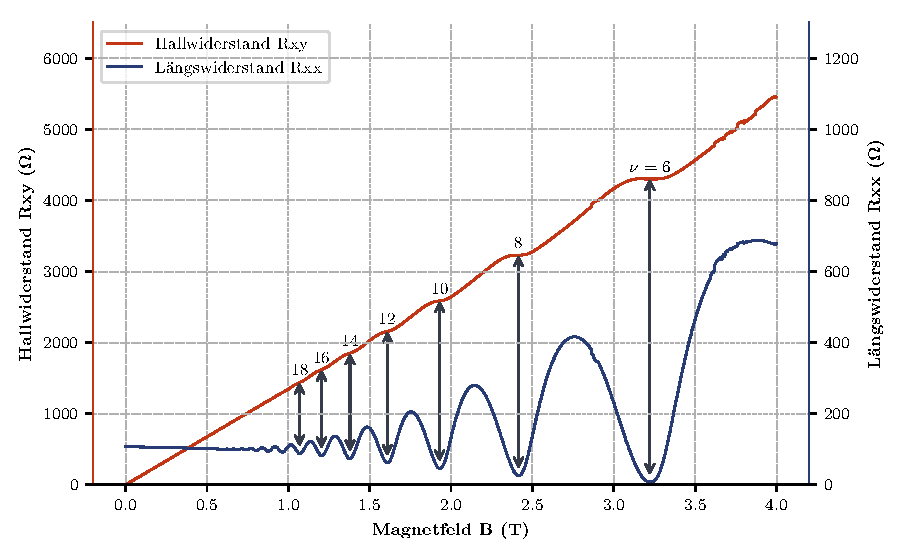
\includegraphics[width=\textwidth]{results_meth_1/P07_0611_0708_0109.pdf}
    \caption{Messung von Längswiderstand und Hallwiderstand in Abhängigkeit des Magnetfelds für Messreihe P07\_1\_A Markiert sind Hallplateaus mit korrespondierenden Minima der SdH-Oszillation und den jeweiligen Füllfaktoren}
	\label{abb:P07_Meth_1}
\end{figure}

Wir konnten so in jeder Messreihe für die Füllfaktoren $\nu = 6$, $\nu = 8$ und noch $\nu = 10 $ (relativ) klare Plateaus messen. Für die Faktoren $\nu = 12, 14, 16, 18$ lassen sich der SdH-Oszillation noch angedeutete Plateaus zuordnen. Diesen Bereich ordnen wir daher dem quantenmechanischen Regime zu und nutzen ihn für diese sowie für die in Abschnitt \ref{subsubsec:Meth_2} beschriebene Methode. \\
\\
Für jedes identifizierte Hallplateau berechnen wir nun die Elektronendichte nach Gl. \ref{eq:ElektrKonz1} \footnote{Die Werte für die Elementarladung und das Plank'sche Wirkungsquantum wurden dem Python-Package Scipy.constants entnommen.}. Die Werte sind für Messreihe P07\_1\_A exemplarisch in Tab. \ref{tab:P07_Meth_1} zu finden. \\
\\
Da die Elektronenkonzentration unabhängig vom Magnetfeld ist, mitteln wir über jedes berücksichtigte Plateau und erhalten Tabelle \ref{tab:Meth_1}. \\ 

Die bestimmten Elektronenkonzentrationen liegen ausgesprochen nah beieinander, es gibt allerdings kleine Abweichungen, die nicht von der Standartabweichung in den einzelnen Messreihen erklärt wird. Auffällig ist, das bei beiden Messungen, bei denen der Längswiderstand zwischen direkt nebeneinander liegenden Kontakten gemessen wurde, eine leicht höhere Elektronenkonzentration festzustellen ist. Insgesamt erscheinen die Abweichungen aber insignifikant. \\

Die Elektronenmobilität lässt sich nun (und auch bei den anderen Ansätzen) mit Gl. \ref{eq:Mobilitaet} aus der E-Konzentration und dem spezifischen Widerstand der Hallgeometrie berechnen. Dabei ist zu beachten, das bei den Messungen [....] mit einem Abstand von zwei Kontakten gemessen wurde. Der spezifische Widerstand ist hier also doppelt so groß. Die Ergebnisse sind ebenfalls Tabelle \ref{tab:Meth_1} zu entnehmen. Im Gegensatz zur E-Konzentration beobachten wir hier sig. Schwankungen. Da diese Schwankungen bei allen Ansätzen gleichermaßen auftreten, diskutieren wir sie in Abschnitt \ref{sec:Schwankungen} zusammenfassend.

\begin{table}
	\centering
	\caption{Bei Messreihe P07\_1\_A beobachtete Hallplateaus mit allen relevanten Größen}
	\begin{tabular}{lrrrr}
\toprule
 $B_{min}[T]$ &    $R_{xy} [\Omega]$ 	&  $R_{xx}[\Omega]$ 	& $\nu$  &$n_e [1/m^2]$\\
\midrule
  1.069 &   1437.48 &   87.656 	&       17.957 &         4.642e+15 \\
  1.204 &   1617.87 &   81.681 	&       15.955 &         4.645e+15 \\
  1.379 &   1852.25 &   73.175 	&       13.936 &         4.647e+15 \\
  1.608 &  2156.23 	&   61.262 	&       11.971 &         4.655e+15 \\
  1.930 & 2585.12 	&    45.183 &        9.985 &         4.660e+15 \\
  2.414 &   3228.92 &    25.370 &        7.994 &         4.666e+15 \\
  3.222 &   4301.67 &     7.432 &        6.001 &         4.675e+15 \\
\bottomrule
\end{tabular}

	\label{tab:P07_Meth_1}
\end{table}
\begin{table}
	\centering
	\caption{Die mit Methode 1 bestimmten E-konzentrationen und -mobilitäten}
	\begin{tabular}{lrrrr}
\toprule
		Messreihe & Längs-WS & E-Dichte & Std-Ab. & E-Mobi. \\
        &  $R_{xx} (B=0) [\Omega]$ & $(\varnothing) [1/\si{m}^2]$  & & $[\si{m^2/V.s}]$ \\
\midrule
 P07\_1\_A  &  106.743 &              4.656e+15 &          1.222e+13 &             15.70 \\
 P07\_1\_B  &  182.622 &              4.634e+15 &          1.501e+13 &             18.44 \\
 P07\_2\_A  &   77.843 &              4.657e+15 &          4.955e+12 &             21.52 \\
 P07\_2\_B  &  160.499 &              4.627e+15 &          1.033e+13 &             21.01 \\
\bottomrule
\end{tabular}

	\label{tab:Meth_1}
\end{table}

\newpage
\subsubsection{Methode 2: Bestimmung der reziproken Periode der SdH-Oszillation} \label{subsubsec:Meth_2}
Die Elektronenkonzentration lässt sich auch mit Gl. \ref{eq:ElektrKonz2} aus der reziproken Periode der SdH-Oszillation berechnen. Dies ist besonders dann interessant, wenn sich den Hallplateaus keine eindeutigen Hallwiderstände mehr zuordnen lassen (was hier auf Füllfaktoren $\nu > 10$ zunehmend zutrifft).

Die rez. Abstände der schon bei Methode 1 genutzten Minima und die aus diesen berechnete Elektronenkonzentration wurden wie schon bei Methode 1 gemittelt und aus dem Mittelwert die Elektronenmobilität bestimmt. Diese Größen sind in den Tabellen \ref{tab:P07_Meth_2} (repräsentativ) und Tab. \ref{tab:Meth_2} zu finden. 

Die beobachtete Elektronenkonzentration / -mobilität liegen mit dieser Methode noch etwas näher beieinander als zuvor, allerdings sind die Standartabweichungen leicht größer geworden. Die zuvor beobachtete leicht höhere E-Konzentration bei den Messungen P07\_1\_A und P07\_2\_A ist in den Werten nicht länger erkennbar. Da sie dennoch mit denen aus Methode 1 in sehr guter Näherung übereinstimmen, erhalten wir gleichermaßen unterschiedliche Werte für die Elektronenmobilität.
 
\begin{figure}[htbp]
	\centering
	%% Creator: Matplotlib, PGF backend
%%
%% To include the figure in your LaTeX document, write
%%   \input{<filename>.pgf}
%%
%% Make sure the required packages are loaded in your preamble
%%   \usepackage{pgf}
%%
%% Figures using additional raster images can only be included by \input if
%% they are in the same directory as the main LaTeX file. For loading figures
%% from other directories you can use the `import` package
%%   \usepackage{import}
%% and then include the figures with
%%   \import{<path to file>}{<filename>.pgf}
%%
%% Matplotlib used the following preamble
%%   \usepackage[utf8x]{inputenc}
%%   \usepackage[T1]{fontenc}
%%
\begingroup%
\makeatletter%
\begin{pgfpicture}%
\pgfpathrectangle{\pgfpointorigin}{\pgfqpoint{4.803151in}{1.979007in}}%
\pgfusepath{use as bounding box, clip}%
\begin{pgfscope}%
\pgfsetbuttcap%
\pgfsetmiterjoin%
\definecolor{currentfill}{rgb}{1.000000,1.000000,1.000000}%
\pgfsetfillcolor{currentfill}%
\pgfsetlinewidth{0.000000pt}%
\definecolor{currentstroke}{rgb}{1.000000,1.000000,1.000000}%
\pgfsetstrokecolor{currentstroke}%
\pgfsetdash{}{0pt}%
\pgfpathmoveto{\pgfqpoint{0.000000in}{0.000000in}}%
\pgfpathlineto{\pgfqpoint{4.803151in}{0.000000in}}%
\pgfpathlineto{\pgfqpoint{4.803151in}{1.979007in}}%
\pgfpathlineto{\pgfqpoint{0.000000in}{1.979007in}}%
\pgfpathclose%
\pgfusepath{fill}%
\end{pgfscope}%
\begin{pgfscope}%
\pgfsetbuttcap%
\pgfsetmiterjoin%
\definecolor{currentfill}{rgb}{1.000000,1.000000,1.000000}%
\pgfsetfillcolor{currentfill}%
\pgfsetlinewidth{0.000000pt}%
\definecolor{currentstroke}{rgb}{0.000000,0.000000,0.000000}%
\pgfsetstrokecolor{currentstroke}%
\pgfsetstrokeopacity{0.000000}%
\pgfsetdash{}{0pt}%
\pgfpathmoveto{\pgfqpoint{0.530975in}{0.451986in}}%
\pgfpathlineto{\pgfqpoint{4.678151in}{0.451986in}}%
\pgfpathlineto{\pgfqpoint{4.678151in}{1.854007in}}%
\pgfpathlineto{\pgfqpoint{0.530975in}{1.854007in}}%
\pgfpathclose%
\pgfusepath{fill}%
\end{pgfscope}%
\begin{pgfscope}%
\pgfsetroundcap%
\pgfsetroundjoin%
\pgfsetlinewidth{0.752812pt}%
\definecolor{currentstroke}{rgb}{0.000000,0.000000,0.000000}%
\pgfsetstrokecolor{currentstroke}%
\pgfsetdash{}{0pt}%
\pgfpathmoveto{\pgfqpoint{2.542562in}{1.326015in}}%
\pgfpathquadraticcurveto{\pgfqpoint{2.709867in}{1.326015in}}{\pgfqpoint{2.877171in}{1.326015in}}%
\pgfusepath{stroke}%
\end{pgfscope}%
\begin{pgfscope}%
\pgfsetroundcap%
\pgfsetroundjoin%
\pgfsetlinewidth{0.752812pt}%
\definecolor{currentstroke}{rgb}{0.000000,0.000000,0.000000}%
\pgfsetstrokecolor{currentstroke}%
\pgfsetdash{}{0pt}%
\pgfpathmoveto{\pgfqpoint{2.206316in}{1.326015in}}%
\pgfpathquadraticcurveto{\pgfqpoint{2.374439in}{1.326015in}}{\pgfqpoint{2.542562in}{1.326015in}}%
\pgfusepath{stroke}%
\end{pgfscope}%
\begin{pgfscope}%
\pgfsetroundcap%
\pgfsetroundjoin%
\pgfsetlinewidth{0.752812pt}%
\definecolor{currentstroke}{rgb}{0.000000,0.000000,0.000000}%
\pgfsetstrokecolor{currentstroke}%
\pgfsetdash{}{0pt}%
\pgfpathmoveto{\pgfqpoint{1.876863in}{1.326015in}}%
\pgfpathquadraticcurveto{\pgfqpoint{2.041589in}{1.326015in}}{\pgfqpoint{2.206316in}{1.326015in}}%
\pgfusepath{stroke}%
\end{pgfscope}%
\begin{pgfscope}%
\pgfsetroundcap%
\pgfsetroundjoin%
\pgfsetlinewidth{0.752812pt}%
\definecolor{currentstroke}{rgb}{0.000000,0.000000,0.000000}%
\pgfsetstrokecolor{currentstroke}%
\pgfsetdash{}{0pt}%
\pgfpathmoveto{\pgfqpoint{1.545867in}{1.326015in}}%
\pgfpathquadraticcurveto{\pgfqpoint{1.711365in}{1.326015in}}{\pgfqpoint{1.876863in}{1.326015in}}%
\pgfusepath{stroke}%
\end{pgfscope}%
\begin{pgfscope}%
\pgfsetroundcap%
\pgfsetroundjoin%
\pgfsetlinewidth{0.752812pt}%
\definecolor{currentstroke}{rgb}{0.000000,0.000000,0.000000}%
\pgfsetstrokecolor{currentstroke}%
\pgfsetdash{}{0pt}%
\pgfpathmoveto{\pgfqpoint{1.214462in}{1.326015in}}%
\pgfpathquadraticcurveto{\pgfqpoint{1.380165in}{1.326015in}}{\pgfqpoint{1.545867in}{1.326015in}}%
\pgfusepath{stroke}%
\end{pgfscope}%
\begin{pgfscope}%
\pgfsetroundcap%
\pgfsetroundjoin%
\pgfsetlinewidth{0.752812pt}%
\definecolor{currentstroke}{rgb}{0.000000,0.000000,0.000000}%
\pgfsetstrokecolor{currentstroke}%
\pgfsetdash{}{0pt}%
\pgfpathmoveto{\pgfqpoint{0.883058in}{1.326015in}}%
\pgfpathquadraticcurveto{\pgfqpoint{1.048760in}{1.326015in}}{\pgfqpoint{1.214462in}{1.326015in}}%
\pgfusepath{stroke}%
\end{pgfscope}%
\begin{pgfscope}%
\pgfpathrectangle{\pgfqpoint{0.530975in}{0.451986in}}{\pgfqpoint{4.147176in}{1.402021in}}%
\pgfusepath{clip}%
\pgfsetbuttcap%
\pgfsetroundjoin%
\pgfsetlinewidth{0.501875pt}%
\definecolor{currentstroke}{rgb}{0.690196,0.690196,0.690196}%
\pgfsetstrokecolor{currentstroke}%
\pgfsetdash{{1.850000pt}{0.800000pt}}{0.000000pt}%
\pgfpathmoveto{\pgfqpoint{0.530975in}{0.451986in}}%
\pgfpathlineto{\pgfqpoint{0.530975in}{1.854007in}}%
\pgfusepath{stroke}%
\end{pgfscope}%
\begin{pgfscope}%
\pgfsetbuttcap%
\pgfsetroundjoin%
\definecolor{currentfill}{rgb}{0.000000,0.000000,0.000000}%
\pgfsetfillcolor{currentfill}%
\pgfsetlinewidth{0.803000pt}%
\definecolor{currentstroke}{rgb}{0.000000,0.000000,0.000000}%
\pgfsetstrokecolor{currentstroke}%
\pgfsetdash{}{0pt}%
\pgfsys@defobject{currentmarker}{\pgfqpoint{0.000000in}{-0.048611in}}{\pgfqpoint{0.000000in}{0.000000in}}{%
\pgfpathmoveto{\pgfqpoint{0.000000in}{0.000000in}}%
\pgfpathlineto{\pgfqpoint{0.000000in}{-0.048611in}}%
\pgfusepath{stroke,fill}%
}%
\begin{pgfscope}%
\pgfsys@transformshift{0.530975in}{0.451986in}%
\pgfsys@useobject{currentmarker}{}%
\end{pgfscope}%
\end{pgfscope}%
\begin{pgfscope}%
\definecolor{textcolor}{rgb}{0.000000,0.000000,0.000000}%
\pgfsetstrokecolor{textcolor}%
\pgfsetfillcolor{textcolor}%
\pgftext[x=0.530975in,y=0.354764in,,top]{\color{textcolor}\rmfamily\fontsize{8.000000}{9.600000}\selectfont \(\displaystyle 0.2\)}%
\end{pgfscope}%
\begin{pgfscope}%
\pgfpathrectangle{\pgfqpoint{0.530975in}{0.451986in}}{\pgfqpoint{4.147176in}{1.402021in}}%
\pgfusepath{clip}%
\pgfsetbuttcap%
\pgfsetroundjoin%
\pgfsetlinewidth{0.501875pt}%
\definecolor{currentstroke}{rgb}{0.690196,0.690196,0.690196}%
\pgfsetstrokecolor{currentstroke}%
\pgfsetdash{{1.850000pt}{0.800000pt}}{0.000000pt}%
\pgfpathmoveto{\pgfqpoint{1.169002in}{0.451986in}}%
\pgfpathlineto{\pgfqpoint{1.169002in}{1.854007in}}%
\pgfusepath{stroke}%
\end{pgfscope}%
\begin{pgfscope}%
\pgfsetbuttcap%
\pgfsetroundjoin%
\definecolor{currentfill}{rgb}{0.000000,0.000000,0.000000}%
\pgfsetfillcolor{currentfill}%
\pgfsetlinewidth{0.803000pt}%
\definecolor{currentstroke}{rgb}{0.000000,0.000000,0.000000}%
\pgfsetstrokecolor{currentstroke}%
\pgfsetdash{}{0pt}%
\pgfsys@defobject{currentmarker}{\pgfqpoint{0.000000in}{-0.048611in}}{\pgfqpoint{0.000000in}{0.000000in}}{%
\pgfpathmoveto{\pgfqpoint{0.000000in}{0.000000in}}%
\pgfpathlineto{\pgfqpoint{0.000000in}{-0.048611in}}%
\pgfusepath{stroke,fill}%
}%
\begin{pgfscope}%
\pgfsys@transformshift{1.169002in}{0.451986in}%
\pgfsys@useobject{currentmarker}{}%
\end{pgfscope}%
\end{pgfscope}%
\begin{pgfscope}%
\definecolor{textcolor}{rgb}{0.000000,0.000000,0.000000}%
\pgfsetstrokecolor{textcolor}%
\pgfsetfillcolor{textcolor}%
\pgftext[x=1.169002in,y=0.354764in,,top]{\color{textcolor}\rmfamily\fontsize{8.000000}{9.600000}\selectfont \(\displaystyle 0.4\)}%
\end{pgfscope}%
\begin{pgfscope}%
\pgfpathrectangle{\pgfqpoint{0.530975in}{0.451986in}}{\pgfqpoint{4.147176in}{1.402021in}}%
\pgfusepath{clip}%
\pgfsetbuttcap%
\pgfsetroundjoin%
\pgfsetlinewidth{0.501875pt}%
\definecolor{currentstroke}{rgb}{0.690196,0.690196,0.690196}%
\pgfsetstrokecolor{currentstroke}%
\pgfsetdash{{1.850000pt}{0.800000pt}}{0.000000pt}%
\pgfpathmoveto{\pgfqpoint{1.807029in}{0.451986in}}%
\pgfpathlineto{\pgfqpoint{1.807029in}{1.854007in}}%
\pgfusepath{stroke}%
\end{pgfscope}%
\begin{pgfscope}%
\pgfsetbuttcap%
\pgfsetroundjoin%
\definecolor{currentfill}{rgb}{0.000000,0.000000,0.000000}%
\pgfsetfillcolor{currentfill}%
\pgfsetlinewidth{0.803000pt}%
\definecolor{currentstroke}{rgb}{0.000000,0.000000,0.000000}%
\pgfsetstrokecolor{currentstroke}%
\pgfsetdash{}{0pt}%
\pgfsys@defobject{currentmarker}{\pgfqpoint{0.000000in}{-0.048611in}}{\pgfqpoint{0.000000in}{0.000000in}}{%
\pgfpathmoveto{\pgfqpoint{0.000000in}{0.000000in}}%
\pgfpathlineto{\pgfqpoint{0.000000in}{-0.048611in}}%
\pgfusepath{stroke,fill}%
}%
\begin{pgfscope}%
\pgfsys@transformshift{1.807029in}{0.451986in}%
\pgfsys@useobject{currentmarker}{}%
\end{pgfscope}%
\end{pgfscope}%
\begin{pgfscope}%
\definecolor{textcolor}{rgb}{0.000000,0.000000,0.000000}%
\pgfsetstrokecolor{textcolor}%
\pgfsetfillcolor{textcolor}%
\pgftext[x=1.807029in,y=0.354764in,,top]{\color{textcolor}\rmfamily\fontsize{8.000000}{9.600000}\selectfont \(\displaystyle 0.6\)}%
\end{pgfscope}%
\begin{pgfscope}%
\pgfpathrectangle{\pgfqpoint{0.530975in}{0.451986in}}{\pgfqpoint{4.147176in}{1.402021in}}%
\pgfusepath{clip}%
\pgfsetbuttcap%
\pgfsetroundjoin%
\pgfsetlinewidth{0.501875pt}%
\definecolor{currentstroke}{rgb}{0.690196,0.690196,0.690196}%
\pgfsetstrokecolor{currentstroke}%
\pgfsetdash{{1.850000pt}{0.800000pt}}{0.000000pt}%
\pgfpathmoveto{\pgfqpoint{2.445056in}{0.451986in}}%
\pgfpathlineto{\pgfqpoint{2.445056in}{1.854007in}}%
\pgfusepath{stroke}%
\end{pgfscope}%
\begin{pgfscope}%
\pgfsetbuttcap%
\pgfsetroundjoin%
\definecolor{currentfill}{rgb}{0.000000,0.000000,0.000000}%
\pgfsetfillcolor{currentfill}%
\pgfsetlinewidth{0.803000pt}%
\definecolor{currentstroke}{rgb}{0.000000,0.000000,0.000000}%
\pgfsetstrokecolor{currentstroke}%
\pgfsetdash{}{0pt}%
\pgfsys@defobject{currentmarker}{\pgfqpoint{0.000000in}{-0.048611in}}{\pgfqpoint{0.000000in}{0.000000in}}{%
\pgfpathmoveto{\pgfqpoint{0.000000in}{0.000000in}}%
\pgfpathlineto{\pgfqpoint{0.000000in}{-0.048611in}}%
\pgfusepath{stroke,fill}%
}%
\begin{pgfscope}%
\pgfsys@transformshift{2.445056in}{0.451986in}%
\pgfsys@useobject{currentmarker}{}%
\end{pgfscope}%
\end{pgfscope}%
\begin{pgfscope}%
\definecolor{textcolor}{rgb}{0.000000,0.000000,0.000000}%
\pgfsetstrokecolor{textcolor}%
\pgfsetfillcolor{textcolor}%
\pgftext[x=2.445056in,y=0.354764in,,top]{\color{textcolor}\rmfamily\fontsize{8.000000}{9.600000}\selectfont \(\displaystyle 0.8\)}%
\end{pgfscope}%
\begin{pgfscope}%
\pgfpathrectangle{\pgfqpoint{0.530975in}{0.451986in}}{\pgfqpoint{4.147176in}{1.402021in}}%
\pgfusepath{clip}%
\pgfsetbuttcap%
\pgfsetroundjoin%
\pgfsetlinewidth{0.501875pt}%
\definecolor{currentstroke}{rgb}{0.690196,0.690196,0.690196}%
\pgfsetstrokecolor{currentstroke}%
\pgfsetdash{{1.850000pt}{0.800000pt}}{0.000000pt}%
\pgfpathmoveto{\pgfqpoint{3.083083in}{0.451986in}}%
\pgfpathlineto{\pgfqpoint{3.083083in}{1.854007in}}%
\pgfusepath{stroke}%
\end{pgfscope}%
\begin{pgfscope}%
\pgfsetbuttcap%
\pgfsetroundjoin%
\definecolor{currentfill}{rgb}{0.000000,0.000000,0.000000}%
\pgfsetfillcolor{currentfill}%
\pgfsetlinewidth{0.803000pt}%
\definecolor{currentstroke}{rgb}{0.000000,0.000000,0.000000}%
\pgfsetstrokecolor{currentstroke}%
\pgfsetdash{}{0pt}%
\pgfsys@defobject{currentmarker}{\pgfqpoint{0.000000in}{-0.048611in}}{\pgfqpoint{0.000000in}{0.000000in}}{%
\pgfpathmoveto{\pgfqpoint{0.000000in}{0.000000in}}%
\pgfpathlineto{\pgfqpoint{0.000000in}{-0.048611in}}%
\pgfusepath{stroke,fill}%
}%
\begin{pgfscope}%
\pgfsys@transformshift{3.083083in}{0.451986in}%
\pgfsys@useobject{currentmarker}{}%
\end{pgfscope}%
\end{pgfscope}%
\begin{pgfscope}%
\definecolor{textcolor}{rgb}{0.000000,0.000000,0.000000}%
\pgfsetstrokecolor{textcolor}%
\pgfsetfillcolor{textcolor}%
\pgftext[x=3.083083in,y=0.354764in,,top]{\color{textcolor}\rmfamily\fontsize{8.000000}{9.600000}\selectfont \(\displaystyle 1.0\)}%
\end{pgfscope}%
\begin{pgfscope}%
\pgfpathrectangle{\pgfqpoint{0.530975in}{0.451986in}}{\pgfqpoint{4.147176in}{1.402021in}}%
\pgfusepath{clip}%
\pgfsetbuttcap%
\pgfsetroundjoin%
\pgfsetlinewidth{0.501875pt}%
\definecolor{currentstroke}{rgb}{0.690196,0.690196,0.690196}%
\pgfsetstrokecolor{currentstroke}%
\pgfsetdash{{1.850000pt}{0.800000pt}}{0.000000pt}%
\pgfpathmoveto{\pgfqpoint{3.721110in}{0.451986in}}%
\pgfpathlineto{\pgfqpoint{3.721110in}{1.854007in}}%
\pgfusepath{stroke}%
\end{pgfscope}%
\begin{pgfscope}%
\pgfsetbuttcap%
\pgfsetroundjoin%
\definecolor{currentfill}{rgb}{0.000000,0.000000,0.000000}%
\pgfsetfillcolor{currentfill}%
\pgfsetlinewidth{0.803000pt}%
\definecolor{currentstroke}{rgb}{0.000000,0.000000,0.000000}%
\pgfsetstrokecolor{currentstroke}%
\pgfsetdash{}{0pt}%
\pgfsys@defobject{currentmarker}{\pgfqpoint{0.000000in}{-0.048611in}}{\pgfqpoint{0.000000in}{0.000000in}}{%
\pgfpathmoveto{\pgfqpoint{0.000000in}{0.000000in}}%
\pgfpathlineto{\pgfqpoint{0.000000in}{-0.048611in}}%
\pgfusepath{stroke,fill}%
}%
\begin{pgfscope}%
\pgfsys@transformshift{3.721110in}{0.451986in}%
\pgfsys@useobject{currentmarker}{}%
\end{pgfscope}%
\end{pgfscope}%
\begin{pgfscope}%
\definecolor{textcolor}{rgb}{0.000000,0.000000,0.000000}%
\pgfsetstrokecolor{textcolor}%
\pgfsetfillcolor{textcolor}%
\pgftext[x=3.721110in,y=0.354764in,,top]{\color{textcolor}\rmfamily\fontsize{8.000000}{9.600000}\selectfont \(\displaystyle 1.2\)}%
\end{pgfscope}%
\begin{pgfscope}%
\pgfpathrectangle{\pgfqpoint{0.530975in}{0.451986in}}{\pgfqpoint{4.147176in}{1.402021in}}%
\pgfusepath{clip}%
\pgfsetbuttcap%
\pgfsetroundjoin%
\pgfsetlinewidth{0.501875pt}%
\definecolor{currentstroke}{rgb}{0.690196,0.690196,0.690196}%
\pgfsetstrokecolor{currentstroke}%
\pgfsetdash{{1.850000pt}{0.800000pt}}{0.000000pt}%
\pgfpathmoveto{\pgfqpoint{4.359137in}{0.451986in}}%
\pgfpathlineto{\pgfqpoint{4.359137in}{1.854007in}}%
\pgfusepath{stroke}%
\end{pgfscope}%
\begin{pgfscope}%
\pgfsetbuttcap%
\pgfsetroundjoin%
\definecolor{currentfill}{rgb}{0.000000,0.000000,0.000000}%
\pgfsetfillcolor{currentfill}%
\pgfsetlinewidth{0.803000pt}%
\definecolor{currentstroke}{rgb}{0.000000,0.000000,0.000000}%
\pgfsetstrokecolor{currentstroke}%
\pgfsetdash{}{0pt}%
\pgfsys@defobject{currentmarker}{\pgfqpoint{0.000000in}{-0.048611in}}{\pgfqpoint{0.000000in}{0.000000in}}{%
\pgfpathmoveto{\pgfqpoint{0.000000in}{0.000000in}}%
\pgfpathlineto{\pgfqpoint{0.000000in}{-0.048611in}}%
\pgfusepath{stroke,fill}%
}%
\begin{pgfscope}%
\pgfsys@transformshift{4.359137in}{0.451986in}%
\pgfsys@useobject{currentmarker}{}%
\end{pgfscope}%
\end{pgfscope}%
\begin{pgfscope}%
\definecolor{textcolor}{rgb}{0.000000,0.000000,0.000000}%
\pgfsetstrokecolor{textcolor}%
\pgfsetfillcolor{textcolor}%
\pgftext[x=4.359137in,y=0.354764in,,top]{\color{textcolor}\rmfamily\fontsize{8.000000}{9.600000}\selectfont \(\displaystyle 1.4\)}%
\end{pgfscope}%
\begin{pgfscope}%
\definecolor{textcolor}{rgb}{0.000000,0.000000,0.000000}%
\pgfsetstrokecolor{textcolor}%
\pgfsetfillcolor{textcolor}%
\pgftext[x=2.604563in,y=0.201084in,,top]{\color{textcolor}\rmfamily\fontsize{8.000000}{9.600000}\selectfont rez. Magnetfeld 1/B [1/T]}%
\end{pgfscope}%
\begin{pgfscope}%
\pgfpathrectangle{\pgfqpoint{0.530975in}{0.451986in}}{\pgfqpoint{4.147176in}{1.402021in}}%
\pgfusepath{clip}%
\pgfsetbuttcap%
\pgfsetroundjoin%
\pgfsetlinewidth{0.501875pt}%
\definecolor{currentstroke}{rgb}{0.690196,0.690196,0.690196}%
\pgfsetstrokecolor{currentstroke}%
\pgfsetdash{{1.850000pt}{0.800000pt}}{0.000000pt}%
\pgfpathmoveto{\pgfqpoint{0.530975in}{0.501793in}}%
\pgfpathlineto{\pgfqpoint{4.678151in}{0.501793in}}%
\pgfusepath{stroke}%
\end{pgfscope}%
\begin{pgfscope}%
\pgfsetbuttcap%
\pgfsetroundjoin%
\definecolor{currentfill}{rgb}{0.000000,0.000000,0.000000}%
\pgfsetfillcolor{currentfill}%
\pgfsetlinewidth{0.803000pt}%
\definecolor{currentstroke}{rgb}{0.000000,0.000000,0.000000}%
\pgfsetstrokecolor{currentstroke}%
\pgfsetdash{}{0pt}%
\pgfsys@defobject{currentmarker}{\pgfqpoint{-0.048611in}{0.000000in}}{\pgfqpoint{0.000000in}{0.000000in}}{%
\pgfpathmoveto{\pgfqpoint{0.000000in}{0.000000in}}%
\pgfpathlineto{\pgfqpoint{-0.048611in}{0.000000in}}%
\pgfusepath{stroke,fill}%
}%
\begin{pgfscope}%
\pgfsys@transformshift{0.530975in}{0.501793in}%
\pgfsys@useobject{currentmarker}{}%
\end{pgfscope}%
\end{pgfscope}%
\begin{pgfscope}%
\definecolor{textcolor}{rgb}{0.000000,0.000000,0.000000}%
\pgfsetstrokecolor{textcolor}%
\pgfsetfillcolor{textcolor}%
\pgftext[x=0.374724in,y=0.463530in,left,base]{\color{textcolor}\rmfamily\fontsize{8.000000}{9.600000}\selectfont \(\displaystyle 0\)}%
\end{pgfscope}%
\begin{pgfscope}%
\pgfpathrectangle{\pgfqpoint{0.530975in}{0.451986in}}{\pgfqpoint{4.147176in}{1.402021in}}%
\pgfusepath{clip}%
\pgfsetbuttcap%
\pgfsetroundjoin%
\pgfsetlinewidth{0.501875pt}%
\definecolor{currentstroke}{rgb}{0.690196,0.690196,0.690196}%
\pgfsetstrokecolor{currentstroke}%
\pgfsetdash{{1.850000pt}{0.800000pt}}{0.000000pt}%
\pgfpathmoveto{\pgfqpoint{0.530975in}{0.876439in}}%
\pgfpathlineto{\pgfqpoint{4.678151in}{0.876439in}}%
\pgfusepath{stroke}%
\end{pgfscope}%
\begin{pgfscope}%
\pgfsetbuttcap%
\pgfsetroundjoin%
\definecolor{currentfill}{rgb}{0.000000,0.000000,0.000000}%
\pgfsetfillcolor{currentfill}%
\pgfsetlinewidth{0.803000pt}%
\definecolor{currentstroke}{rgb}{0.000000,0.000000,0.000000}%
\pgfsetstrokecolor{currentstroke}%
\pgfsetdash{}{0pt}%
\pgfsys@defobject{currentmarker}{\pgfqpoint{-0.048611in}{0.000000in}}{\pgfqpoint{0.000000in}{0.000000in}}{%
\pgfpathmoveto{\pgfqpoint{0.000000in}{0.000000in}}%
\pgfpathlineto{\pgfqpoint{-0.048611in}{0.000000in}}%
\pgfusepath{stroke,fill}%
}%
\begin{pgfscope}%
\pgfsys@transformshift{0.530975in}{0.876439in}%
\pgfsys@useobject{currentmarker}{}%
\end{pgfscope}%
\end{pgfscope}%
\begin{pgfscope}%
\definecolor{textcolor}{rgb}{0.000000,0.000000,0.000000}%
\pgfsetstrokecolor{textcolor}%
\pgfsetfillcolor{textcolor}%
\pgftext[x=0.256667in,y=0.838177in,left,base]{\color{textcolor}\rmfamily\fontsize{8.000000}{9.600000}\selectfont \(\displaystyle 200\)}%
\end{pgfscope}%
\begin{pgfscope}%
\pgfpathrectangle{\pgfqpoint{0.530975in}{0.451986in}}{\pgfqpoint{4.147176in}{1.402021in}}%
\pgfusepath{clip}%
\pgfsetbuttcap%
\pgfsetroundjoin%
\pgfsetlinewidth{0.501875pt}%
\definecolor{currentstroke}{rgb}{0.690196,0.690196,0.690196}%
\pgfsetstrokecolor{currentstroke}%
\pgfsetdash{{1.850000pt}{0.800000pt}}{0.000000pt}%
\pgfpathmoveto{\pgfqpoint{0.530975in}{1.251086in}}%
\pgfpathlineto{\pgfqpoint{4.678151in}{1.251086in}}%
\pgfusepath{stroke}%
\end{pgfscope}%
\begin{pgfscope}%
\pgfsetbuttcap%
\pgfsetroundjoin%
\definecolor{currentfill}{rgb}{0.000000,0.000000,0.000000}%
\pgfsetfillcolor{currentfill}%
\pgfsetlinewidth{0.803000pt}%
\definecolor{currentstroke}{rgb}{0.000000,0.000000,0.000000}%
\pgfsetstrokecolor{currentstroke}%
\pgfsetdash{}{0pt}%
\pgfsys@defobject{currentmarker}{\pgfqpoint{-0.048611in}{0.000000in}}{\pgfqpoint{0.000000in}{0.000000in}}{%
\pgfpathmoveto{\pgfqpoint{0.000000in}{0.000000in}}%
\pgfpathlineto{\pgfqpoint{-0.048611in}{0.000000in}}%
\pgfusepath{stroke,fill}%
}%
\begin{pgfscope}%
\pgfsys@transformshift{0.530975in}{1.251086in}%
\pgfsys@useobject{currentmarker}{}%
\end{pgfscope}%
\end{pgfscope}%
\begin{pgfscope}%
\definecolor{textcolor}{rgb}{0.000000,0.000000,0.000000}%
\pgfsetstrokecolor{textcolor}%
\pgfsetfillcolor{textcolor}%
\pgftext[x=0.256667in,y=1.212823in,left,base]{\color{textcolor}\rmfamily\fontsize{8.000000}{9.600000}\selectfont \(\displaystyle 400\)}%
\end{pgfscope}%
\begin{pgfscope}%
\pgfpathrectangle{\pgfqpoint{0.530975in}{0.451986in}}{\pgfqpoint{4.147176in}{1.402021in}}%
\pgfusepath{clip}%
\pgfsetbuttcap%
\pgfsetroundjoin%
\pgfsetlinewidth{0.501875pt}%
\definecolor{currentstroke}{rgb}{0.690196,0.690196,0.690196}%
\pgfsetstrokecolor{currentstroke}%
\pgfsetdash{{1.850000pt}{0.800000pt}}{0.000000pt}%
\pgfpathmoveto{\pgfqpoint{0.530975in}{1.625732in}}%
\pgfpathlineto{\pgfqpoint{4.678151in}{1.625732in}}%
\pgfusepath{stroke}%
\end{pgfscope}%
\begin{pgfscope}%
\pgfsetbuttcap%
\pgfsetroundjoin%
\definecolor{currentfill}{rgb}{0.000000,0.000000,0.000000}%
\pgfsetfillcolor{currentfill}%
\pgfsetlinewidth{0.803000pt}%
\definecolor{currentstroke}{rgb}{0.000000,0.000000,0.000000}%
\pgfsetstrokecolor{currentstroke}%
\pgfsetdash{}{0pt}%
\pgfsys@defobject{currentmarker}{\pgfqpoint{-0.048611in}{0.000000in}}{\pgfqpoint{0.000000in}{0.000000in}}{%
\pgfpathmoveto{\pgfqpoint{0.000000in}{0.000000in}}%
\pgfpathlineto{\pgfqpoint{-0.048611in}{0.000000in}}%
\pgfusepath{stroke,fill}%
}%
\begin{pgfscope}%
\pgfsys@transformshift{0.530975in}{1.625732in}%
\pgfsys@useobject{currentmarker}{}%
\end{pgfscope}%
\end{pgfscope}%
\begin{pgfscope}%
\definecolor{textcolor}{rgb}{0.000000,0.000000,0.000000}%
\pgfsetstrokecolor{textcolor}%
\pgfsetfillcolor{textcolor}%
\pgftext[x=0.256667in,y=1.587470in,left,base]{\color{textcolor}\rmfamily\fontsize{8.000000}{9.600000}\selectfont \(\displaystyle 600\)}%
\end{pgfscope}%
\begin{pgfscope}%
\definecolor{textcolor}{rgb}{0.000000,0.000000,0.000000}%
\pgfsetstrokecolor{textcolor}%
\pgfsetfillcolor{textcolor}%
\pgftext[x=0.201111in,y=1.152996in,,bottom,rotate=90.000000]{\color{textcolor}\rmfamily\fontsize{8.000000}{9.600000}\selectfont Längswiderstand \(\displaystyle R_{xx} [\Omega]\)}%
\end{pgfscope}%
\begin{pgfscope}%
\pgfpathrectangle{\pgfqpoint{0.530975in}{0.451986in}}{\pgfqpoint{4.147176in}{1.402021in}}%
\pgfusepath{clip}%
\pgfsetrectcap%
\pgfsetroundjoin%
\pgfsetlinewidth{1.003750pt}%
\definecolor{currentstroke}{rgb}{0.760784,0.211765,0.086275}%
\pgfsetstrokecolor{currentstroke}%
\pgfsetdash{}{0pt}%
\pgfpathmoveto{\pgfqpoint{4.688151in}{0.690375in}}%
\pgfpathlineto{\pgfqpoint{4.633119in}{0.689526in}}%
\pgfpathlineto{\pgfqpoint{4.619074in}{0.688754in}}%
\pgfpathlineto{\pgfqpoint{4.591232in}{0.687941in}}%
\pgfpathlineto{\pgfqpoint{4.577434in}{0.687214in}}%
\pgfpathlineto{\pgfqpoint{4.443783in}{0.688254in}}%
\pgfpathlineto{\pgfqpoint{4.430836in}{0.689131in}}%
\pgfpathlineto{\pgfqpoint{4.405162in}{0.689987in}}%
\pgfpathlineto{\pgfqpoint{4.392433in}{0.690678in}}%
\pgfpathlineto{\pgfqpoint{4.311418in}{0.690148in}}%
\pgfpathlineto{\pgfqpoint{4.299212in}{0.689195in}}%
\pgfpathlineto{\pgfqpoint{4.275002in}{0.688098in}}%
\pgfpathlineto{\pgfqpoint{4.245110in}{0.685895in}}%
\pgfpathlineto{\pgfqpoint{4.221489in}{0.685004in}}%
\pgfpathlineto{\pgfqpoint{4.203941in}{0.684536in}}%
\pgfpathlineto{\pgfqpoint{4.163544in}{0.684849in}}%
\pgfpathlineto{\pgfqpoint{4.152140in}{0.685553in}}%
\pgfpathlineto{\pgfqpoint{4.129515in}{0.686633in}}%
\pgfpathlineto{\pgfqpoint{4.123896in}{0.687899in}}%
\pgfpathlineto{\pgfqpoint{4.112703in}{0.687899in}}%
\pgfpathlineto{\pgfqpoint{4.107129in}{0.689294in}}%
\pgfpathlineto{\pgfqpoint{4.096024in}{0.689294in}}%
\pgfpathlineto{\pgfqpoint{4.090494in}{0.690540in}}%
\pgfpathlineto{\pgfqpoint{4.063059in}{0.691632in}}%
\pgfpathlineto{\pgfqpoint{4.052185in}{0.692359in}}%
\pgfpathlineto{\pgfqpoint{3.998656in}{0.692100in}}%
\pgfpathlineto{\pgfqpoint{3.988115in}{0.691141in}}%
\pgfpathlineto{\pgfqpoint{3.982865in}{0.691141in}}%
\pgfpathlineto{\pgfqpoint{3.977628in}{0.689871in}}%
\pgfpathlineto{\pgfqpoint{3.961998in}{0.689871in}}%
\pgfpathlineto{\pgfqpoint{3.956814in}{0.688320in}}%
\pgfpathlineto{\pgfqpoint{3.946487in}{0.687514in}}%
\pgfpathlineto{\pgfqpoint{3.925988in}{0.685143in}}%
\pgfpathlineto{\pgfqpoint{3.915817in}{0.684451in}}%
\pgfpathlineto{\pgfqpoint{3.905696in}{0.683759in}}%
\pgfpathlineto{\pgfqpoint{3.885608in}{0.682704in}}%
\pgfpathlineto{\pgfqpoint{3.875638in}{0.682042in}}%
\pgfpathlineto{\pgfqpoint{3.826530in}{0.683125in}}%
\pgfpathlineto{\pgfqpoint{3.821686in}{0.684412in}}%
\pgfpathlineto{\pgfqpoint{3.807224in}{0.685234in}}%
\pgfpathlineto{\pgfqpoint{3.788107in}{0.687897in}}%
\pgfpathlineto{\pgfqpoint{3.783357in}{0.687897in}}%
\pgfpathlineto{\pgfqpoint{3.778618in}{0.689798in}}%
\pgfpathlineto{\pgfqpoint{3.764471in}{0.690763in}}%
\pgfpathlineto{\pgfqpoint{3.750427in}{0.692557in}}%
\pgfpathlineto{\pgfqpoint{3.736484in}{0.694035in}}%
\pgfpathlineto{\pgfqpoint{3.718050in}{0.695650in}}%
\pgfpathlineto{\pgfqpoint{3.668256in}{0.694723in}}%
\pgfpathlineto{\pgfqpoint{3.646048in}{0.692578in}}%
\pgfpathlineto{\pgfqpoint{3.641638in}{0.692578in}}%
\pgfpathlineto{\pgfqpoint{3.637238in}{0.690684in}}%
\pgfpathlineto{\pgfqpoint{3.628469in}{0.690684in}}%
\pgfpathlineto{\pgfqpoint{3.624100in}{0.688548in}}%
\pgfpathlineto{\pgfqpoint{3.615393in}{0.688548in}}%
\pgfpathlineto{\pgfqpoint{3.611054in}{0.686317in}}%
\pgfpathlineto{\pgfqpoint{3.602407in}{0.686317in}}%
\pgfpathlineto{\pgfqpoint{3.598099in}{0.684170in}}%
\pgfpathlineto{\pgfqpoint{3.585234in}{0.683157in}}%
\pgfpathlineto{\pgfqpoint{3.572458in}{0.680515in}}%
\pgfpathlineto{\pgfqpoint{3.559770in}{0.679867in}}%
\pgfpathlineto{\pgfqpoint{3.547169in}{0.678531in}}%
\pgfpathlineto{\pgfqpoint{3.513987in}{0.678970in}}%
\pgfpathlineto{\pgfqpoint{3.505785in}{0.680022in}}%
\pgfpathlineto{\pgfqpoint{3.497620in}{0.680861in}}%
\pgfpathlineto{\pgfqpoint{3.481401in}{0.683831in}}%
\pgfpathlineto{\pgfqpoint{3.473346in}{0.683831in}}%
\pgfpathlineto{\pgfqpoint{3.469332in}{0.686348in}}%
\pgfpathlineto{\pgfqpoint{3.461332in}{0.686348in}}%
\pgfpathlineto{\pgfqpoint{3.457345in}{0.688969in}}%
\pgfpathlineto{\pgfqpoint{3.449397in}{0.688969in}}%
\pgfpathlineto{\pgfqpoint{3.445437in}{0.691658in}}%
\pgfpathlineto{\pgfqpoint{3.441485in}{0.691658in}}%
\pgfpathlineto{\pgfqpoint{3.433608in}{0.694271in}}%
\pgfpathlineto{\pgfqpoint{3.429683in}{0.694271in}}%
\pgfpathlineto{\pgfqpoint{3.421858in}{0.696740in}}%
\pgfpathlineto{\pgfqpoint{3.410186in}{0.697742in}}%
\pgfpathlineto{\pgfqpoint{3.398591in}{0.700438in}}%
\pgfpathlineto{\pgfqpoint{3.379434in}{0.701506in}}%
\pgfpathlineto{\pgfqpoint{3.368041in}{0.702032in}}%
\pgfpathlineto{\pgfqpoint{3.345475in}{0.701419in}}%
\pgfpathlineto{\pgfqpoint{3.341743in}{0.700146in}}%
\pgfpathlineto{\pgfqpoint{3.334302in}{0.700146in}}%
\pgfpathlineto{\pgfqpoint{3.330593in}{0.698478in}}%
\pgfpathlineto{\pgfqpoint{3.319516in}{0.698478in}}%
\pgfpathlineto{\pgfqpoint{3.315840in}{0.696245in}}%
\pgfpathlineto{\pgfqpoint{3.308510in}{0.696245in}}%
\pgfpathlineto{\pgfqpoint{3.304857in}{0.693685in}}%
\pgfpathlineto{\pgfqpoint{3.301212in}{0.693685in}}%
\pgfpathlineto{\pgfqpoint{3.293945in}{0.690852in}}%
\pgfpathlineto{\pgfqpoint{3.290323in}{0.690852in}}%
\pgfpathlineto{\pgfqpoint{3.283102in}{0.687939in}}%
\pgfpathlineto{\pgfqpoint{3.279503in}{0.687939in}}%
\pgfpathlineto{\pgfqpoint{3.272328in}{0.684895in}}%
\pgfpathlineto{\pgfqpoint{3.265184in}{0.684895in}}%
\pgfpathlineto{\pgfqpoint{3.261623in}{0.681945in}}%
\pgfpathlineto{\pgfqpoint{3.254523in}{0.681945in}}%
\pgfpathlineto{\pgfqpoint{3.250985in}{0.679345in}}%
\pgfpathlineto{\pgfqpoint{3.243930in}{0.679345in}}%
\pgfpathlineto{\pgfqpoint{3.240414in}{0.677055in}}%
\pgfpathlineto{\pgfqpoint{3.233403in}{0.676164in}}%
\pgfpathlineto{\pgfqpoint{3.226422in}{0.675274in}}%
\pgfpathlineto{\pgfqpoint{3.222943in}{0.675274in}}%
\pgfpathlineto{\pgfqpoint{3.219470in}{0.673984in}}%
\pgfpathlineto{\pgfqpoint{3.181747in}{0.674491in}}%
\pgfpathlineto{\pgfqpoint{3.178360in}{0.675981in}}%
\pgfpathlineto{\pgfqpoint{3.168241in}{0.675981in}}%
\pgfpathlineto{\pgfqpoint{3.164881in}{0.678149in}}%
\pgfpathlineto{\pgfqpoint{3.161529in}{0.678149in}}%
\pgfpathlineto{\pgfqpoint{3.154845in}{0.680933in}}%
\pgfpathlineto{\pgfqpoint{3.151513in}{0.680933in}}%
\pgfpathlineto{\pgfqpoint{3.144869in}{0.684056in}}%
\pgfpathlineto{\pgfqpoint{3.141558in}{0.684056in}}%
\pgfpathlineto{\pgfqpoint{3.134955in}{0.687583in}}%
\pgfpathlineto{\pgfqpoint{3.131664in}{0.687583in}}%
\pgfpathlineto{\pgfqpoint{3.128379in}{0.691246in}}%
\pgfpathlineto{\pgfqpoint{3.118565in}{0.691246in}}%
\pgfpathlineto{\pgfqpoint{3.115307in}{0.694944in}}%
\pgfpathlineto{\pgfqpoint{3.108810in}{0.694944in}}%
\pgfpathlineto{\pgfqpoint{3.105571in}{0.698548in}}%
\pgfpathlineto{\pgfqpoint{3.102339in}{0.698548in}}%
\pgfpathlineto{\pgfqpoint{3.095895in}{0.701815in}}%
\pgfpathlineto{\pgfqpoint{3.089476in}{0.701815in}}%
\pgfpathlineto{\pgfqpoint{3.086276in}{0.704875in}}%
\pgfpathlineto{\pgfqpoint{3.079896in}{0.704875in}}%
\pgfpathlineto{\pgfqpoint{3.073541in}{0.707549in}}%
\pgfpathlineto{\pgfqpoint{3.070373in}{0.707549in}}%
\pgfpathlineto{\pgfqpoint{3.067212in}{0.709662in}}%
\pgfpathlineto{\pgfqpoint{3.060907in}{0.709662in}}%
\pgfpathlineto{\pgfqpoint{3.057764in}{0.711211in}}%
\pgfpathlineto{\pgfqpoint{3.042143in}{0.712224in}}%
\pgfpathlineto{\pgfqpoint{3.032845in}{0.712576in}}%
\pgfpathlineto{\pgfqpoint{3.005275in}{0.709838in}}%
\pgfpathlineto{\pgfqpoint{3.002241in}{0.707738in}}%
\pgfpathlineto{\pgfqpoint{2.996192in}{0.707738in}}%
\pgfpathlineto{\pgfqpoint{2.993176in}{0.705158in}}%
\pgfpathlineto{\pgfqpoint{2.984164in}{0.705158in}}%
\pgfpathlineto{\pgfqpoint{2.981172in}{0.702131in}}%
\pgfpathlineto{\pgfqpoint{2.975204in}{0.702131in}}%
\pgfpathlineto{\pgfqpoint{2.972229in}{0.698769in}}%
\pgfpathlineto{\pgfqpoint{2.966296in}{0.698769in}}%
\pgfpathlineto{\pgfqpoint{2.963338in}{0.695047in}}%
\pgfpathlineto{\pgfqpoint{2.957439in}{0.695047in}}%
\pgfpathlineto{\pgfqpoint{2.954498in}{0.691156in}}%
\pgfpathlineto{\pgfqpoint{2.948633in}{0.691156in}}%
\pgfpathlineto{\pgfqpoint{2.945709in}{0.687211in}}%
\pgfpathlineto{\pgfqpoint{2.939877in}{0.687211in}}%
\pgfpathlineto{\pgfqpoint{2.936970in}{0.683305in}}%
\pgfpathlineto{\pgfqpoint{2.931172in}{0.683305in}}%
\pgfpathlineto{\pgfqpoint{2.928281in}{0.679505in}}%
\pgfpathlineto{\pgfqpoint{2.922516in}{0.679505in}}%
\pgfpathlineto{\pgfqpoint{2.919641in}{0.675960in}}%
\pgfpathlineto{\pgfqpoint{2.913909in}{0.675960in}}%
\pgfpathlineto{\pgfqpoint{2.911051in}{0.672749in}}%
\pgfpathlineto{\pgfqpoint{2.905351in}{0.672749in}}%
\pgfpathlineto{\pgfqpoint{2.899673in}{0.670083in}}%
\pgfpathlineto{\pgfqpoint{2.896842in}{0.670083in}}%
\pgfpathlineto{\pgfqpoint{2.894016in}{0.667997in}}%
\pgfpathlineto{\pgfqpoint{2.888380in}{0.667997in}}%
\pgfpathlineto{\pgfqpoint{2.885570in}{0.666656in}}%
\pgfpathlineto{\pgfqpoint{2.855005in}{0.666968in}}%
\pgfpathlineto{\pgfqpoint{2.852257in}{0.668678in}}%
\pgfpathlineto{\pgfqpoint{2.846777in}{0.668678in}}%
\pgfpathlineto{\pgfqpoint{2.844044in}{0.671095in}}%
\pgfpathlineto{\pgfqpoint{2.838594in}{0.671095in}}%
\pgfpathlineto{\pgfqpoint{2.835877in}{0.674184in}}%
\pgfpathlineto{\pgfqpoint{2.827755in}{0.674184in}}%
\pgfpathlineto{\pgfqpoint{2.825057in}{0.677890in}}%
\pgfpathlineto{\pgfqpoint{2.819677in}{0.677890in}}%
\pgfpathlineto{\pgfqpoint{2.816995in}{0.682101in}}%
\pgfpathlineto{\pgfqpoint{2.814317in}{0.682101in}}%
\pgfpathlineto{\pgfqpoint{2.808976in}{0.686621in}}%
\pgfpathlineto{\pgfqpoint{2.806313in}{0.686621in}}%
\pgfpathlineto{\pgfqpoint{2.801002in}{0.691398in}}%
\pgfpathlineto{\pgfqpoint{2.795710in}{0.691398in}}%
\pgfpathlineto{\pgfqpoint{2.793071in}{0.696227in}}%
\pgfpathlineto{\pgfqpoint{2.787807in}{0.696227in}}%
\pgfpathlineto{\pgfqpoint{2.785183in}{0.701063in}}%
\pgfpathlineto{\pgfqpoint{2.779948in}{0.701063in}}%
\pgfpathlineto{\pgfqpoint{2.777338in}{0.705806in}}%
\pgfpathlineto{\pgfqpoint{2.772131in}{0.705806in}}%
\pgfpathlineto{\pgfqpoint{2.769535in}{0.710338in}}%
\pgfpathlineto{\pgfqpoint{2.764357in}{0.710338in}}%
\pgfpathlineto{\pgfqpoint{2.761774in}{0.714470in}}%
\pgfpathlineto{\pgfqpoint{2.756624in}{0.714470in}}%
\pgfpathlineto{\pgfqpoint{2.751492in}{0.718308in}}%
\pgfpathlineto{\pgfqpoint{2.748933in}{0.718308in}}%
\pgfpathlineto{\pgfqpoint{2.743828in}{0.721609in}}%
\pgfpathlineto{\pgfqpoint{2.741283in}{0.721609in}}%
\pgfpathlineto{\pgfqpoint{2.736205in}{0.724408in}}%
\pgfpathlineto{\pgfqpoint{2.733674in}{0.724408in}}%
\pgfpathlineto{\pgfqpoint{2.726105in}{0.726695in}}%
\pgfpathlineto{\pgfqpoint{2.723591in}{0.726695in}}%
\pgfpathlineto{\pgfqpoint{2.721082in}{0.728287in}}%
\pgfpathlineto{\pgfqpoint{2.711088in}{0.729355in}}%
\pgfpathlineto{\pgfqpoint{2.696230in}{0.729477in}}%
\pgfpathlineto{\pgfqpoint{2.671811in}{0.725067in}}%
\pgfpathlineto{\pgfqpoint{2.669393in}{0.722506in}}%
\pgfpathlineto{\pgfqpoint{2.664568in}{0.722506in}}%
\pgfpathlineto{\pgfqpoint{2.662162in}{0.719365in}}%
\pgfpathlineto{\pgfqpoint{2.657363in}{0.719365in}}%
\pgfpathlineto{\pgfqpoint{2.652580in}{0.715723in}}%
\pgfpathlineto{\pgfqpoint{2.650195in}{0.715723in}}%
\pgfpathlineto{\pgfqpoint{2.645437in}{0.711838in}}%
\pgfpathlineto{\pgfqpoint{2.643064in}{0.711838in}}%
\pgfpathlineto{\pgfqpoint{2.640696in}{0.707436in}}%
\pgfpathlineto{\pgfqpoint{2.635970in}{0.707436in}}%
\pgfpathlineto{\pgfqpoint{2.633614in}{0.702858in}}%
\pgfpathlineto{\pgfqpoint{2.628913in}{0.702858in}}%
\pgfpathlineto{\pgfqpoint{2.626568in}{0.697905in}}%
\pgfpathlineto{\pgfqpoint{2.619559in}{0.697905in}}%
\pgfpathlineto{\pgfqpoint{2.617231in}{0.692832in}}%
\pgfpathlineto{\pgfqpoint{2.614906in}{0.692832in}}%
\pgfpathlineto{\pgfqpoint{2.610269in}{0.687811in}}%
\pgfpathlineto{\pgfqpoint{2.607956in}{0.687811in}}%
\pgfpathlineto{\pgfqpoint{2.603343in}{0.682836in}}%
\pgfpathlineto{\pgfqpoint{2.601042in}{0.682836in}}%
\pgfpathlineto{\pgfqpoint{2.596452in}{0.677921in}}%
\pgfpathlineto{\pgfqpoint{2.594163in}{0.677921in}}%
\pgfpathlineto{\pgfqpoint{2.589596in}{0.673317in}}%
\pgfpathlineto{\pgfqpoint{2.585045in}{0.673317in}}%
\pgfpathlineto{\pgfqpoint{2.582775in}{0.668952in}}%
\pgfpathlineto{\pgfqpoint{2.578247in}{0.668952in}}%
\pgfpathlineto{\pgfqpoint{2.575988in}{0.665049in}}%
\pgfpathlineto{\pgfqpoint{2.571483in}{0.665049in}}%
\pgfpathlineto{\pgfqpoint{2.569236in}{0.661556in}}%
\pgfpathlineto{\pgfqpoint{2.564753in}{0.661556in}}%
\pgfpathlineto{\pgfqpoint{2.562517in}{0.658777in}}%
\pgfpathlineto{\pgfqpoint{2.558056in}{0.658777in}}%
\pgfpathlineto{\pgfqpoint{2.555832in}{0.656723in}}%
\pgfpathlineto{\pgfqpoint{2.549180in}{0.656020in}}%
\pgfpathlineto{\pgfqpoint{2.542562in}{0.654799in}}%
\pgfpathlineto{\pgfqpoint{2.531604in}{0.655097in}}%
\pgfpathlineto{\pgfqpoint{2.527246in}{0.656282in}}%
\pgfpathlineto{\pgfqpoint{2.522903in}{0.657292in}}%
\pgfpathlineto{\pgfqpoint{2.518573in}{0.658302in}}%
\pgfpathlineto{\pgfqpoint{2.516414in}{0.658302in}}%
\pgfpathlineto{\pgfqpoint{2.514258in}{0.661083in}}%
\pgfpathlineto{\pgfqpoint{2.512106in}{0.661083in}}%
\pgfpathlineto{\pgfqpoint{2.509958in}{0.664662in}}%
\pgfpathlineto{\pgfqpoint{2.505671in}{0.664662in}}%
\pgfpathlineto{\pgfqpoint{2.503533in}{0.668950in}}%
\pgfpathlineto{\pgfqpoint{2.499267in}{0.668950in}}%
\pgfpathlineto{\pgfqpoint{2.497140in}{0.673759in}}%
\pgfpathlineto{\pgfqpoint{2.490778in}{0.673759in}}%
\pgfpathlineto{\pgfqpoint{2.488664in}{0.679142in}}%
\pgfpathlineto{\pgfqpoint{2.484447in}{0.679142in}}%
\pgfpathlineto{\pgfqpoint{2.482343in}{0.684959in}}%
\pgfpathlineto{\pgfqpoint{2.480243in}{0.684959in}}%
\pgfpathlineto{\pgfqpoint{2.476053in}{0.690984in}}%
\pgfpathlineto{\pgfqpoint{2.471877in}{0.690984in}}%
\pgfpathlineto{\pgfqpoint{2.469794in}{0.697132in}}%
\pgfpathlineto{\pgfqpoint{2.465637in}{0.697132in}}%
\pgfpathlineto{\pgfqpoint{2.463564in}{0.703431in}}%
\pgfpathlineto{\pgfqpoint{2.459428in}{0.703431in}}%
\pgfpathlineto{\pgfqpoint{2.457365in}{0.709675in}}%
\pgfpathlineto{\pgfqpoint{2.453249in}{0.709675in}}%
\pgfpathlineto{\pgfqpoint{2.451196in}{0.715748in}}%
\pgfpathlineto{\pgfqpoint{2.447099in}{0.715748in}}%
\pgfpathlineto{\pgfqpoint{2.445056in}{0.721637in}}%
\pgfpathlineto{\pgfqpoint{2.440979in}{0.721637in}}%
\pgfpathlineto{\pgfqpoint{2.438945in}{0.727291in}}%
\pgfpathlineto{\pgfqpoint{2.434888in}{0.727291in}}%
\pgfpathlineto{\pgfqpoint{2.432864in}{0.732631in}}%
\pgfpathlineto{\pgfqpoint{2.426812in}{0.732631in}}%
\pgfpathlineto{\pgfqpoint{2.424801in}{0.737457in}}%
\pgfpathlineto{\pgfqpoint{2.422793in}{0.737457in}}%
\pgfpathlineto{\pgfqpoint{2.420789in}{0.741864in}}%
\pgfpathlineto{\pgfqpoint{2.416789in}{0.741864in}}%
\pgfpathlineto{\pgfqpoint{2.412802in}{0.745783in}}%
\pgfpathlineto{\pgfqpoint{2.410813in}{0.745783in}}%
\pgfpathlineto{\pgfqpoint{2.408827in}{0.749172in}}%
\pgfpathlineto{\pgfqpoint{2.402889in}{0.749172in}}%
\pgfpathlineto{\pgfqpoint{2.400916in}{0.752087in}}%
\pgfpathlineto{\pgfqpoint{2.398946in}{0.752087in}}%
\pgfpathlineto{\pgfqpoint{2.393054in}{0.754421in}}%
\pgfpathlineto{\pgfqpoint{2.391096in}{0.754421in}}%
\pgfpathlineto{\pgfqpoint{2.389141in}{0.756200in}}%
\pgfpathlineto{\pgfqpoint{2.385241in}{0.756820in}}%
\pgfpathlineto{\pgfqpoint{2.379413in}{0.757749in}}%
\pgfpathlineto{\pgfqpoint{2.371685in}{0.758105in}}%
\pgfpathlineto{\pgfqpoint{2.362093in}{0.757523in}}%
\pgfpathlineto{\pgfqpoint{2.358276in}{0.756423in}}%
\pgfpathlineto{\pgfqpoint{2.352574in}{0.754805in}}%
\pgfpathlineto{\pgfqpoint{2.350679in}{0.754805in}}%
\pgfpathlineto{\pgfqpoint{2.348787in}{0.752624in}}%
\pgfpathlineto{\pgfqpoint{2.345012in}{0.752624in}}%
\pgfpathlineto{\pgfqpoint{2.335624in}{0.746765in}}%
\pgfpathlineto{\pgfqpoint{2.333755in}{0.746765in}}%
\pgfpathlineto{\pgfqpoint{2.331889in}{0.743196in}}%
\pgfpathlineto{\pgfqpoint{2.328165in}{0.743196in}}%
\pgfpathlineto{\pgfqpoint{2.326308in}{0.739101in}}%
\pgfpathlineto{\pgfqpoint{2.322601in}{0.739101in}}%
\pgfpathlineto{\pgfqpoint{2.320752in}{0.734607in}}%
\pgfpathlineto{\pgfqpoint{2.317063in}{0.734607in}}%
\pgfpathlineto{\pgfqpoint{2.313384in}{0.729780in}}%
\pgfpathlineto{\pgfqpoint{2.311549in}{0.729780in}}%
\pgfpathlineto{\pgfqpoint{2.307887in}{0.724597in}}%
\pgfpathlineto{\pgfqpoint{2.306061in}{0.724597in}}%
\pgfpathlineto{\pgfqpoint{2.302415in}{0.719211in}}%
\pgfpathlineto{\pgfqpoint{2.300597in}{0.719211in}}%
\pgfpathlineto{\pgfqpoint{2.296968in}{0.713530in}}%
\pgfpathlineto{\pgfqpoint{2.293350in}{0.713530in}}%
\pgfpathlineto{\pgfqpoint{2.291546in}{0.707599in}}%
\pgfpathlineto{\pgfqpoint{2.287944in}{0.707599in}}%
\pgfpathlineto{\pgfqpoint{2.286147in}{0.701440in}}%
\pgfpathlineto{\pgfqpoint{2.282562in}{0.701440in}}%
\pgfpathlineto{\pgfqpoint{2.280773in}{0.695348in}}%
\pgfpathlineto{\pgfqpoint{2.277204in}{0.695348in}}%
\pgfpathlineto{\pgfqpoint{2.275424in}{0.689148in}}%
\pgfpathlineto{\pgfqpoint{2.271870in}{0.689148in}}%
\pgfpathlineto{\pgfqpoint{2.270098in}{0.682925in}}%
\pgfpathlineto{\pgfqpoint{2.266560in}{0.682925in}}%
\pgfpathlineto{\pgfqpoint{2.263033in}{0.676840in}}%
\pgfpathlineto{\pgfqpoint{2.261274in}{0.676840in}}%
\pgfpathlineto{\pgfqpoint{2.259517in}{0.671089in}}%
\pgfpathlineto{\pgfqpoint{2.256011in}{0.671089in}}%
\pgfpathlineto{\pgfqpoint{2.254262in}{0.665445in}}%
\pgfpathlineto{\pgfqpoint{2.250771in}{0.665445in}}%
\pgfpathlineto{\pgfqpoint{2.249030in}{0.660171in}}%
\pgfpathlineto{\pgfqpoint{2.245555in}{0.660171in}}%
\pgfpathlineto{\pgfqpoint{2.242090in}{0.655238in}}%
\pgfpathlineto{\pgfqpoint{2.240361in}{0.655238in}}%
\pgfpathlineto{\pgfqpoint{2.236912in}{0.650893in}}%
\pgfpathlineto{\pgfqpoint{2.235191in}{0.650893in}}%
\pgfpathlineto{\pgfqpoint{2.231757in}{0.647090in}}%
\pgfpathlineto{\pgfqpoint{2.230043in}{0.647090in}}%
\pgfpathlineto{\pgfqpoint{2.228332in}{0.643954in}}%
\pgfpathlineto{\pgfqpoint{2.224918in}{0.643954in}}%
\pgfpathlineto{\pgfqpoint{2.223214in}{0.641470in}}%
\pgfpathlineto{\pgfqpoint{2.218119in}{0.641470in}}%
\pgfpathlineto{\pgfqpoint{2.216426in}{0.639759in}}%
\pgfpathlineto{\pgfqpoint{2.197959in}{0.640643in}}%
\pgfpathlineto{\pgfqpoint{2.194633in}{0.641560in}}%
\pgfpathlineto{\pgfqpoint{2.192973in}{0.641560in}}%
\pgfpathlineto{\pgfqpoint{2.191316in}{0.644203in}}%
\pgfpathlineto{\pgfqpoint{2.188009in}{0.644203in}}%
\pgfpathlineto{\pgfqpoint{2.186359in}{0.647613in}}%
\pgfpathlineto{\pgfqpoint{2.183066in}{0.647613in}}%
\pgfpathlineto{\pgfqpoint{2.181423in}{0.651997in}}%
\pgfpathlineto{\pgfqpoint{2.179783in}{0.651997in}}%
\pgfpathlineto{\pgfqpoint{2.176509in}{0.656976in}}%
\pgfpathlineto{\pgfqpoint{2.174876in}{0.656976in}}%
\pgfpathlineto{\pgfqpoint{2.171616in}{0.662728in}}%
\pgfpathlineto{\pgfqpoint{2.168365in}{0.662728in}}%
\pgfpathlineto{\pgfqpoint{2.166743in}{0.668935in}}%
\pgfpathlineto{\pgfqpoint{2.163507in}{0.668935in}}%
\pgfpathlineto{\pgfqpoint{2.161892in}{0.675684in}}%
\pgfpathlineto{\pgfqpoint{2.158669in}{0.675684in}}%
\pgfpathlineto{\pgfqpoint{2.157061in}{0.682794in}}%
\pgfpathlineto{\pgfqpoint{2.153851in}{0.682794in}}%
\pgfpathlineto{\pgfqpoint{2.152250in}{0.690298in}}%
\pgfpathlineto{\pgfqpoint{2.147460in}{0.690298in}}%
\pgfpathlineto{\pgfqpoint{2.145868in}{0.697958in}}%
\pgfpathlineto{\pgfqpoint{2.144278in}{0.697958in}}%
\pgfpathlineto{\pgfqpoint{2.141105in}{0.705675in}}%
\pgfpathlineto{\pgfqpoint{2.139522in}{0.705675in}}%
\pgfpathlineto{\pgfqpoint{2.136362in}{0.713530in}}%
\pgfpathlineto{\pgfqpoint{2.134786in}{0.713530in}}%
\pgfpathlineto{\pgfqpoint{2.131639in}{0.721242in}}%
\pgfpathlineto{\pgfqpoint{2.130069in}{0.721242in}}%
\pgfpathlineto{\pgfqpoint{2.126936in}{0.729035in}}%
\pgfpathlineto{\pgfqpoint{2.123811in}{0.729035in}}%
\pgfpathlineto{\pgfqpoint{2.122253in}{0.736374in}}%
\pgfpathlineto{\pgfqpoint{2.119141in}{0.736374in}}%
\pgfpathlineto{\pgfqpoint{2.117589in}{0.743702in}}%
\pgfpathlineto{\pgfqpoint{2.114490in}{0.743702in}}%
\pgfpathlineto{\pgfqpoint{2.112944in}{0.750691in}}%
\pgfpathlineto{\pgfqpoint{2.109859in}{0.750691in}}%
\pgfpathlineto{\pgfqpoint{2.108319in}{0.757407in}}%
\pgfpathlineto{\pgfqpoint{2.105247in}{0.757407in}}%
\pgfpathlineto{\pgfqpoint{2.103714in}{0.763721in}}%
\pgfpathlineto{\pgfqpoint{2.100654in}{0.763721in}}%
\pgfpathlineto{\pgfqpoint{2.099127in}{0.769691in}}%
\pgfpathlineto{\pgfqpoint{2.096080in}{0.769691in}}%
\pgfpathlineto{\pgfqpoint{2.094559in}{0.775219in}}%
\pgfpathlineto{\pgfqpoint{2.091525in}{0.775219in}}%
\pgfpathlineto{\pgfqpoint{2.090011in}{0.780382in}}%
\pgfpathlineto{\pgfqpoint{2.086988in}{0.780382in}}%
\pgfpathlineto{\pgfqpoint{2.085480in}{0.785054in}}%
\pgfpathlineto{\pgfqpoint{2.082471in}{0.785054in}}%
\pgfpathlineto{\pgfqpoint{2.079469in}{0.789340in}}%
\pgfpathlineto{\pgfqpoint{2.077972in}{0.789340in}}%
\pgfpathlineto{\pgfqpoint{2.076476in}{0.793073in}}%
\pgfpathlineto{\pgfqpoint{2.073491in}{0.793073in}}%
\pgfpathlineto{\pgfqpoint{2.072002in}{0.796304in}}%
\pgfpathlineto{\pgfqpoint{2.069029in}{0.796304in}}%
\pgfpathlineto{\pgfqpoint{2.067546in}{0.799148in}}%
\pgfpathlineto{\pgfqpoint{2.064585in}{0.799148in}}%
\pgfpathlineto{\pgfqpoint{2.063108in}{0.801448in}}%
\pgfpathlineto{\pgfqpoint{2.058688in}{0.801448in}}%
\pgfpathlineto{\pgfqpoint{2.057219in}{0.803274in}}%
\pgfpathlineto{\pgfqpoint{2.054286in}{0.803274in}}%
\pgfpathlineto{\pgfqpoint{2.051361in}{0.804571in}}%
\pgfpathlineto{\pgfqpoint{2.044084in}{0.805818in}}%
\pgfpathlineto{\pgfqpoint{2.032542in}{0.805125in}}%
\pgfpathlineto{\pgfqpoint{2.028246in}{0.803355in}}%
\pgfpathlineto{\pgfqpoint{2.021123in}{0.800609in}}%
\pgfpathlineto{\pgfqpoint{2.019705in}{0.800609in}}%
\pgfpathlineto{\pgfqpoint{2.012639in}{0.795435in}}%
\pgfpathlineto{\pgfqpoint{2.011231in}{0.795435in}}%
\pgfpathlineto{\pgfqpoint{2.009826in}{0.792136in}}%
\pgfpathlineto{\pgfqpoint{2.007020in}{0.792136in}}%
\pgfpathlineto{\pgfqpoint{2.005620in}{0.788493in}}%
\pgfpathlineto{\pgfqpoint{2.001431in}{0.788493in}}%
\pgfpathlineto{\pgfqpoint{2.000038in}{0.784428in}}%
\pgfpathlineto{\pgfqpoint{1.997259in}{0.784428in}}%
\pgfpathlineto{\pgfqpoint{1.995871in}{0.780056in}}%
\pgfpathlineto{\pgfqpoint{1.994486in}{0.780056in}}%
\pgfpathlineto{\pgfqpoint{1.993103in}{0.775294in}}%
\pgfpathlineto{\pgfqpoint{1.990341in}{0.775294in}}%
\pgfpathlineto{\pgfqpoint{1.988963in}{0.770174in}}%
\pgfpathlineto{\pgfqpoint{1.986212in}{0.770174in}}%
\pgfpathlineto{\pgfqpoint{1.984840in}{0.764753in}}%
\pgfpathlineto{\pgfqpoint{1.980733in}{0.764753in}}%
\pgfpathlineto{\pgfqpoint{1.979367in}{0.759001in}}%
\pgfpathlineto{\pgfqpoint{1.978003in}{0.759001in}}%
\pgfpathlineto{\pgfqpoint{1.975281in}{0.753119in}}%
\pgfpathlineto{\pgfqpoint{1.973923in}{0.753119in}}%
\pgfpathlineto{\pgfqpoint{1.971212in}{0.746770in}}%
\pgfpathlineto{\pgfqpoint{1.968507in}{0.746770in}}%
\pgfpathlineto{\pgfqpoint{1.967158in}{0.740285in}}%
\pgfpathlineto{\pgfqpoint{1.964464in}{0.740285in}}%
\pgfpathlineto{\pgfqpoint{1.963120in}{0.733656in}}%
\pgfpathlineto{\pgfqpoint{1.960436in}{0.733656in}}%
\pgfpathlineto{\pgfqpoint{1.959097in}{0.726910in}}%
\pgfpathlineto{\pgfqpoint{1.956425in}{0.726910in}}%
\pgfpathlineto{\pgfqpoint{1.955091in}{0.719938in}}%
\pgfpathlineto{\pgfqpoint{1.953759in}{0.719938in}}%
\pgfpathlineto{\pgfqpoint{1.951099in}{0.712833in}}%
\pgfpathlineto{\pgfqpoint{1.948447in}{0.712833in}}%
\pgfpathlineto{\pgfqpoint{1.947124in}{0.705636in}}%
\pgfpathlineto{\pgfqpoint{1.944482in}{0.705636in}}%
\pgfpathlineto{\pgfqpoint{1.941846in}{0.698336in}}%
\pgfpathlineto{\pgfqpoint{1.940531in}{0.698336in}}%
\pgfpathlineto{\pgfqpoint{1.939218in}{0.691203in}}%
\pgfpathlineto{\pgfqpoint{1.936596in}{0.691203in}}%
\pgfpathlineto{\pgfqpoint{1.935288in}{0.683934in}}%
\pgfpathlineto{\pgfqpoint{1.932676in}{0.683934in}}%
\pgfpathlineto{\pgfqpoint{1.931373in}{0.676973in}}%
\pgfpathlineto{\pgfqpoint{1.927473in}{0.676973in}}%
\pgfpathlineto{\pgfqpoint{1.926176in}{0.670008in}}%
\pgfpathlineto{\pgfqpoint{1.924881in}{0.670008in}}%
\pgfpathlineto{\pgfqpoint{1.922296in}{0.663176in}}%
\pgfpathlineto{\pgfqpoint{1.919717in}{0.663176in}}%
\pgfpathlineto{\pgfqpoint{1.918430in}{0.656665in}}%
\pgfpathlineto{\pgfqpoint{1.917145in}{0.656665in}}%
\pgfpathlineto{\pgfqpoint{1.915862in}{0.650434in}}%
\pgfpathlineto{\pgfqpoint{1.913299in}{0.650434in}}%
\pgfpathlineto{\pgfqpoint{1.910744in}{0.644414in}}%
\pgfpathlineto{\pgfqpoint{1.908194in}{0.644414in}}%
\pgfpathlineto{\pgfqpoint{1.906922in}{0.638938in}}%
\pgfpathlineto{\pgfqpoint{1.904382in}{0.638938in}}%
\pgfpathlineto{\pgfqpoint{1.903115in}{0.633895in}}%
\pgfpathlineto{\pgfqpoint{1.901849in}{0.633895in}}%
\pgfpathlineto{\pgfqpoint{1.898061in}{0.629411in}}%
\pgfpathlineto{\pgfqpoint{1.894287in}{0.625551in}}%
\pgfpathlineto{\pgfqpoint{1.893032in}{0.625551in}}%
\pgfpathlineto{\pgfqpoint{1.891779in}{0.622143in}}%
\pgfpathlineto{\pgfqpoint{1.889278in}{0.622143in}}%
\pgfpathlineto{\pgfqpoint{1.888029in}{0.619631in}}%
\pgfpathlineto{\pgfqpoint{1.885537in}{0.619631in}}%
\pgfpathlineto{\pgfqpoint{1.883051in}{0.617756in}}%
\pgfpathlineto{\pgfqpoint{1.878097in}{0.616757in}}%
\pgfpathlineto{\pgfqpoint{1.873168in}{0.616852in}}%
\pgfpathlineto{\pgfqpoint{1.867041in}{0.618770in}}%
\pgfpathlineto{\pgfqpoint{1.864601in}{0.621174in}}%
\pgfpathlineto{\pgfqpoint{1.863383in}{0.621174in}}%
\pgfpathlineto{\pgfqpoint{1.862167in}{0.624537in}}%
\pgfpathlineto{\pgfqpoint{1.859739in}{0.624537in}}%
\pgfpathlineto{\pgfqpoint{1.858527in}{0.628684in}}%
\pgfpathlineto{\pgfqpoint{1.854900in}{0.628684in}}%
\pgfpathlineto{\pgfqpoint{1.853695in}{0.633652in}}%
\pgfpathlineto{\pgfqpoint{1.852490in}{0.633652in}}%
\pgfpathlineto{\pgfqpoint{1.846490in}{0.645835in}}%
\pgfpathlineto{\pgfqpoint{1.845295in}{0.645835in}}%
\pgfpathlineto{\pgfqpoint{1.844101in}{0.652851in}}%
\pgfpathlineto{\pgfqpoint{1.840527in}{0.652851in}}%
\pgfpathlineto{\pgfqpoint{1.839339in}{0.660581in}}%
\pgfpathlineto{\pgfqpoint{1.836967in}{0.660581in}}%
\pgfpathlineto{\pgfqpoint{1.835783in}{0.668655in}}%
\pgfpathlineto{\pgfqpoint{1.833419in}{0.668655in}}%
\pgfpathlineto{\pgfqpoint{1.832240in}{0.677055in}}%
\pgfpathlineto{\pgfqpoint{1.829885in}{0.677055in}}%
\pgfpathlineto{\pgfqpoint{1.828709in}{0.685879in}}%
\pgfpathlineto{\pgfqpoint{1.827535in}{0.685879in}}%
\pgfpathlineto{\pgfqpoint{1.825192in}{0.695013in}}%
\pgfpathlineto{\pgfqpoint{1.822854in}{0.695013in}}%
\pgfpathlineto{\pgfqpoint{1.821687in}{0.704233in}}%
\pgfpathlineto{\pgfqpoint{1.819358in}{0.704233in}}%
\pgfpathlineto{\pgfqpoint{1.818195in}{0.713505in}}%
\pgfpathlineto{\pgfqpoint{1.815874in}{0.713505in}}%
\pgfpathlineto{\pgfqpoint{1.814716in}{0.723006in}}%
\pgfpathlineto{\pgfqpoint{1.812403in}{0.723006in}}%
\pgfpathlineto{\pgfqpoint{1.811249in}{0.732290in}}%
\pgfpathlineto{\pgfqpoint{1.807795in}{0.732290in}}%
\pgfpathlineto{\pgfqpoint{1.806646in}{0.741705in}}%
\pgfpathlineto{\pgfqpoint{1.805499in}{0.741705in}}%
\pgfpathlineto{\pgfqpoint{1.800923in}{0.759851in}}%
\pgfpathlineto{\pgfqpoint{1.798644in}{0.759851in}}%
\pgfpathlineto{\pgfqpoint{1.797506in}{0.768650in}}%
\pgfpathlineto{\pgfqpoint{1.794101in}{0.768650in}}%
\pgfpathlineto{\pgfqpoint{1.792969in}{0.777548in}}%
\pgfpathlineto{\pgfqpoint{1.790708in}{0.777548in}}%
\pgfpathlineto{\pgfqpoint{1.789580in}{0.785908in}}%
\pgfpathlineto{\pgfqpoint{1.787327in}{0.785908in}}%
\pgfpathlineto{\pgfqpoint{1.786203in}{0.794083in}}%
\pgfpathlineto{\pgfqpoint{1.785080in}{0.794083in}}%
\pgfpathlineto{\pgfqpoint{1.781719in}{0.801931in}}%
\pgfpathlineto{\pgfqpoint{1.780602in}{0.801931in}}%
\pgfpathlineto{\pgfqpoint{1.778370in}{0.809585in}}%
\pgfpathlineto{\pgfqpoint{1.777257in}{0.809585in}}%
\pgfpathlineto{\pgfqpoint{1.775033in}{0.816848in}}%
\pgfpathlineto{\pgfqpoint{1.773924in}{0.816848in}}%
\pgfpathlineto{\pgfqpoint{1.771708in}{0.823749in}}%
\pgfpathlineto{\pgfqpoint{1.770602in}{0.823749in}}%
\pgfpathlineto{\pgfqpoint{1.768395in}{0.830324in}}%
\pgfpathlineto{\pgfqpoint{1.767293in}{0.830324in}}%
\pgfpathlineto{\pgfqpoint{1.765093in}{0.836547in}}%
\pgfpathlineto{\pgfqpoint{1.763995in}{0.836547in}}%
\pgfpathlineto{\pgfqpoint{1.761803in}{0.842348in}}%
\pgfpathlineto{\pgfqpoint{1.759615in}{0.842348in}}%
\pgfpathlineto{\pgfqpoint{1.757433in}{0.847826in}}%
\pgfpathlineto{\pgfqpoint{1.755257in}{0.852953in}}%
\pgfpathlineto{\pgfqpoint{1.754170in}{0.852953in}}%
\pgfpathlineto{\pgfqpoint{1.752001in}{0.857735in}}%
\pgfpathlineto{\pgfqpoint{1.750918in}{0.857735in}}%
\pgfpathlineto{\pgfqpoint{1.748756in}{0.862203in}}%
\pgfpathlineto{\pgfqpoint{1.746600in}{0.862203in}}%
\pgfpathlineto{\pgfqpoint{1.744448in}{0.866215in}}%
\pgfpathlineto{\pgfqpoint{1.743374in}{0.866215in}}%
\pgfpathlineto{\pgfqpoint{1.741230in}{0.869874in}}%
\pgfpathlineto{\pgfqpoint{1.740160in}{0.869874in}}%
\pgfpathlineto{\pgfqpoint{1.738023in}{0.873150in}}%
\pgfpathlineto{\pgfqpoint{1.732703in}{0.878509in}}%
\pgfpathlineto{\pgfqpoint{1.730583in}{0.878509in}}%
\pgfpathlineto{\pgfqpoint{1.728469in}{0.880650in}}%
\pgfpathlineto{\pgfqpoint{1.727413in}{0.880650in}}%
\pgfpathlineto{\pgfqpoint{1.725306in}{0.882477in}}%
\pgfpathlineto{\pgfqpoint{1.715882in}{0.885586in}}%
\pgfpathlineto{\pgfqpoint{1.702440in}{0.884708in}}%
\pgfpathlineto{\pgfqpoint{1.690207in}{0.878344in}}%
\pgfpathlineto{\pgfqpoint{1.688184in}{0.875967in}}%
\pgfpathlineto{\pgfqpoint{1.686166in}{0.875967in}}%
\pgfpathlineto{\pgfqpoint{1.684152in}{0.873223in}}%
\pgfpathlineto{\pgfqpoint{1.683147in}{0.873223in}}%
\pgfpathlineto{\pgfqpoint{1.681140in}{0.870203in}}%
\pgfpathlineto{\pgfqpoint{1.680138in}{0.870203in}}%
\pgfpathlineto{\pgfqpoint{1.678138in}{0.866766in}}%
\pgfpathlineto{\pgfqpoint{1.677140in}{0.866766in}}%
\pgfpathlineto{\pgfqpoint{1.675146in}{0.863102in}}%
\pgfpathlineto{\pgfqpoint{1.674151in}{0.863102in}}%
\pgfpathlineto{\pgfqpoint{1.669192in}{0.854890in}}%
\pgfpathlineto{\pgfqpoint{1.668204in}{0.854890in}}%
\pgfpathlineto{\pgfqpoint{1.666230in}{0.850285in}}%
\pgfpathlineto{\pgfqpoint{1.665245in}{0.850285in}}%
\pgfpathlineto{\pgfqpoint{1.663278in}{0.845480in}}%
\pgfpathlineto{\pgfqpoint{1.662296in}{0.845480in}}%
\pgfpathlineto{\pgfqpoint{1.660336in}{0.840409in}}%
\pgfpathlineto{\pgfqpoint{1.658379in}{0.840409in}}%
\pgfpathlineto{\pgfqpoint{1.656428in}{0.834998in}}%
\pgfpathlineto{\pgfqpoint{1.651567in}{0.823580in}}%
\pgfpathlineto{\pgfqpoint{1.650598in}{0.823580in}}%
\pgfpathlineto{\pgfqpoint{1.648663in}{0.817556in}}%
\pgfpathlineto{\pgfqpoint{1.647698in}{0.817556in}}%
\pgfpathlineto{\pgfqpoint{1.645769in}{0.811268in}}%
\pgfpathlineto{\pgfqpoint{1.643845in}{0.811268in}}%
\pgfpathlineto{\pgfqpoint{1.641925in}{0.804693in}}%
\pgfpathlineto{\pgfqpoint{1.640967in}{0.804693in}}%
\pgfpathlineto{\pgfqpoint{1.639053in}{0.797968in}}%
\pgfpathlineto{\pgfqpoint{1.634288in}{0.784100in}}%
\pgfpathlineto{\pgfqpoint{1.632389in}{0.784100in}}%
\pgfpathlineto{\pgfqpoint{1.630494in}{0.776901in}}%
\pgfpathlineto{\pgfqpoint{1.629548in}{0.776901in}}%
\pgfpathlineto{\pgfqpoint{1.627660in}{0.769509in}}%
\pgfpathlineto{\pgfqpoint{1.626717in}{0.769509in}}%
\pgfpathlineto{\pgfqpoint{1.624834in}{0.761968in}}%
\pgfpathlineto{\pgfqpoint{1.623895in}{0.761968in}}%
\pgfpathlineto{\pgfqpoint{1.622018in}{0.754361in}}%
\pgfpathlineto{\pgfqpoint{1.619211in}{0.746701in}}%
\pgfpathlineto{\pgfqpoint{1.618278in}{0.746701in}}%
\pgfpathlineto{\pgfqpoint{1.616414in}{0.738884in}}%
\pgfpathlineto{\pgfqpoint{1.615483in}{0.738884in}}%
\pgfpathlineto{\pgfqpoint{1.610845in}{0.723113in}}%
\pgfpathlineto{\pgfqpoint{1.609920in}{0.723113in}}%
\pgfpathlineto{\pgfqpoint{1.608074in}{0.715186in}}%
\pgfpathlineto{\pgfqpoint{1.607153in}{0.715186in}}%
\pgfpathlineto{\pgfqpoint{1.605312in}{0.707144in}}%
\pgfpathlineto{\pgfqpoint{1.603476in}{0.707144in}}%
\pgfpathlineto{\pgfqpoint{1.601644in}{0.699246in}}%
\pgfpathlineto{\pgfqpoint{1.597080in}{0.683472in}}%
\pgfpathlineto{\pgfqpoint{1.596170in}{0.683472in}}%
\pgfpathlineto{\pgfqpoint{1.594353in}{0.675833in}}%
\pgfpathlineto{\pgfqpoint{1.592540in}{0.675833in}}%
\pgfpathlineto{\pgfqpoint{1.590731in}{0.668113in}}%
\pgfpathlineto{\pgfqpoint{1.589828in}{0.668113in}}%
\pgfpathlineto{\pgfqpoint{1.588025in}{0.660580in}}%
\pgfpathlineto{\pgfqpoint{1.587125in}{0.660580in}}%
\pgfpathlineto{\pgfqpoint{1.585327in}{0.653032in}}%
\pgfpathlineto{\pgfqpoint{1.584430in}{0.653032in}}%
\pgfpathlineto{\pgfqpoint{1.582638in}{0.645864in}}%
\pgfpathlineto{\pgfqpoint{1.581743in}{0.645864in}}%
\pgfpathlineto{\pgfqpoint{1.579957in}{0.638956in}}%
\pgfpathlineto{\pgfqpoint{1.579066in}{0.638956in}}%
\pgfpathlineto{\pgfqpoint{1.577285in}{0.632285in}}%
\pgfpathlineto{\pgfqpoint{1.576396in}{0.632285in}}%
\pgfpathlineto{\pgfqpoint{1.574621in}{0.625853in}}%
\pgfpathlineto{\pgfqpoint{1.573735in}{0.625853in}}%
\pgfpathlineto{\pgfqpoint{1.571966in}{0.619764in}}%
\pgfpathlineto{\pgfqpoint{1.571083in}{0.619764in}}%
\pgfpathlineto{\pgfqpoint{1.569319in}{0.614080in}}%
\pgfpathlineto{\pgfqpoint{1.567559in}{0.614080in}}%
\pgfpathlineto{\pgfqpoint{1.565803in}{0.608868in}}%
\pgfpathlineto{\pgfqpoint{1.561428in}{0.599594in}}%
\pgfpathlineto{\pgfqpoint{1.560556in}{0.599594in}}%
\pgfpathlineto{\pgfqpoint{1.558815in}{0.595835in}}%
\pgfpathlineto{\pgfqpoint{1.557945in}{0.595835in}}%
\pgfpathlineto{\pgfqpoint{1.556209in}{0.592615in}}%
\pgfpathlineto{\pgfqpoint{1.554476in}{0.592615in}}%
\pgfpathlineto{\pgfqpoint{1.552747in}{0.589931in}}%
\pgfpathlineto{\pgfqpoint{1.548441in}{0.586904in}}%
\pgfpathlineto{\pgfqpoint{1.539044in}{0.587985in}}%
\pgfpathlineto{\pgfqpoint{1.537347in}{0.589913in}}%
\pgfpathlineto{\pgfqpoint{1.536500in}{0.589913in}}%
\pgfpathlineto{\pgfqpoint{1.534808in}{0.592734in}}%
\pgfpathlineto{\pgfqpoint{1.533964in}{0.592734in}}%
\pgfpathlineto{\pgfqpoint{1.532277in}{0.596297in}}%
\pgfpathlineto{\pgfqpoint{1.531435in}{0.596297in}}%
\pgfpathlineto{\pgfqpoint{1.527238in}{0.606124in}}%
\pgfpathlineto{\pgfqpoint{1.526401in}{0.606124in}}%
\pgfpathlineto{\pgfqpoint{1.524730in}{0.612094in}}%
\pgfpathlineto{\pgfqpoint{1.523896in}{0.612094in}}%
\pgfpathlineto{\pgfqpoint{1.522230in}{0.618736in}}%
\pgfpathlineto{\pgfqpoint{1.521399in}{0.618736in}}%
\pgfpathlineto{\pgfqpoint{1.519738in}{0.626154in}}%
\pgfpathlineto{\pgfqpoint{1.518080in}{0.626154in}}%
\pgfpathlineto{\pgfqpoint{1.516426in}{0.634148in}}%
\pgfpathlineto{\pgfqpoint{1.515600in}{0.634148in}}%
\pgfpathlineto{\pgfqpoint{1.513951in}{0.642778in}}%
\pgfpathlineto{\pgfqpoint{1.513128in}{0.642778in}}%
\pgfpathlineto{\pgfqpoint{1.511484in}{0.651631in}}%
\pgfpathlineto{\pgfqpoint{1.509024in}{0.661113in}}%
\pgfpathlineto{\pgfqpoint{1.508206in}{0.661113in}}%
\pgfpathlineto{\pgfqpoint{1.506572in}{0.670829in}}%
\pgfpathlineto{\pgfqpoint{1.505756in}{0.670829in}}%
\pgfpathlineto{\pgfqpoint{1.504127in}{0.680967in}}%
\pgfpathlineto{\pgfqpoint{1.503314in}{0.680967in}}%
\pgfpathlineto{\pgfqpoint{1.501690in}{0.691270in}}%
\pgfpathlineto{\pgfqpoint{1.500879in}{0.691270in}}%
\pgfpathlineto{\pgfqpoint{1.499259in}{0.701762in}}%
\pgfpathlineto{\pgfqpoint{1.498451in}{0.701762in}}%
\pgfpathlineto{\pgfqpoint{1.496837in}{0.712567in}}%
\pgfpathlineto{\pgfqpoint{1.496031in}{0.712567in}}%
\pgfpathlineto{\pgfqpoint{1.492013in}{0.734133in}}%
\pgfpathlineto{\pgfqpoint{1.491212in}{0.734133in}}%
\pgfpathlineto{\pgfqpoint{1.489612in}{0.744959in}}%
\pgfpathlineto{\pgfqpoint{1.488813in}{0.744959in}}%
\pgfpathlineto{\pgfqpoint{1.487218in}{0.755790in}}%
\pgfpathlineto{\pgfqpoint{1.485626in}{0.755790in}}%
\pgfpathlineto{\pgfqpoint{1.483244in}{0.777358in}}%
\pgfpathlineto{\pgfqpoint{1.481660in}{0.777358in}}%
\pgfpathlineto{\pgfqpoint{1.480080in}{0.787764in}}%
\pgfpathlineto{\pgfqpoint{1.479290in}{0.787764in}}%
\pgfpathlineto{\pgfqpoint{1.477714in}{0.798252in}}%
\pgfpathlineto{\pgfqpoint{1.476927in}{0.798252in}}%
\pgfpathlineto{\pgfqpoint{1.475356in}{0.808396in}}%
\pgfpathlineto{\pgfqpoint{1.473788in}{0.808396in}}%
\pgfpathlineto{\pgfqpoint{1.472223in}{0.818689in}}%
\pgfpathlineto{\pgfqpoint{1.468323in}{0.838482in}}%
\pgfpathlineto{\pgfqpoint{1.467546in}{0.838482in}}%
\pgfpathlineto{\pgfqpoint{1.463669in}{0.857162in}}%
\pgfpathlineto{\pgfqpoint{1.462124in}{0.857162in}}%
\pgfpathlineto{\pgfqpoint{1.460582in}{0.866234in}}%
\pgfpathlineto{\pgfqpoint{1.459812in}{0.866234in}}%
\pgfpathlineto{\pgfqpoint{1.458274in}{0.875160in}}%
\pgfpathlineto{\pgfqpoint{1.457506in}{0.875160in}}%
\pgfpathlineto{\pgfqpoint{1.455973in}{0.883679in}}%
\pgfpathlineto{\pgfqpoint{1.455208in}{0.883679in}}%
\pgfpathlineto{\pgfqpoint{1.453679in}{0.892111in}}%
\pgfpathlineto{\pgfqpoint{1.452916in}{0.892111in}}%
\pgfpathlineto{\pgfqpoint{1.449111in}{0.908125in}}%
\pgfpathlineto{\pgfqpoint{1.448352in}{0.908125in}}%
\pgfpathlineto{\pgfqpoint{1.446837in}{0.915781in}}%
\pgfpathlineto{\pgfqpoint{1.446081in}{0.915781in}}%
\pgfpathlineto{\pgfqpoint{1.444570in}{0.923028in}}%
\pgfpathlineto{\pgfqpoint{1.443816in}{0.923028in}}%
\pgfpathlineto{\pgfqpoint{1.442309in}{0.930145in}}%
\pgfpathlineto{\pgfqpoint{1.441557in}{0.930145in}}%
\pgfpathlineto{\pgfqpoint{1.437807in}{0.943716in}}%
\pgfpathlineto{\pgfqpoint{1.437060in}{0.943716in}}%
\pgfpathlineto{\pgfqpoint{1.433332in}{0.956158in}}%
\pgfpathlineto{\pgfqpoint{1.432588in}{0.956158in}}%
\pgfpathlineto{\pgfqpoint{1.428882in}{0.967508in}}%
\pgfpathlineto{\pgfqpoint{1.428143in}{0.967508in}}%
\pgfpathlineto{\pgfqpoint{1.426667in}{0.972751in}}%
\pgfpathlineto{\pgfqpoint{1.425193in}{0.972751in}}%
\pgfpathlineto{\pgfqpoint{1.423723in}{0.977871in}}%
\pgfpathlineto{\pgfqpoint{1.422989in}{0.977871in}}%
\pgfpathlineto{\pgfqpoint{1.421522in}{0.982599in}}%
\pgfpathlineto{\pgfqpoint{1.420790in}{0.982599in}}%
\pgfpathlineto{\pgfqpoint{1.419328in}{0.987243in}}%
\pgfpathlineto{\pgfqpoint{1.418598in}{0.987243in}}%
\pgfpathlineto{\pgfqpoint{1.417140in}{0.991422in}}%
\pgfpathlineto{\pgfqpoint{1.416412in}{0.991422in}}%
\pgfpathlineto{\pgfqpoint{1.414959in}{0.995344in}}%
\pgfpathlineto{\pgfqpoint{1.414233in}{0.995344in}}%
\pgfpathlineto{\pgfqpoint{1.412783in}{0.999164in}}%
\pgfpathlineto{\pgfqpoint{1.412060in}{0.999164in}}%
\pgfpathlineto{\pgfqpoint{1.410614in}{1.002644in}}%
\pgfpathlineto{\pgfqpoint{1.409893in}{1.002644in}}%
\pgfpathlineto{\pgfqpoint{1.408451in}{1.005958in}}%
\pgfpathlineto{\pgfqpoint{1.407732in}{1.005958in}}%
\pgfpathlineto{\pgfqpoint{1.406295in}{1.008882in}}%
\pgfpathlineto{\pgfqpoint{1.405577in}{1.008882in}}%
\pgfpathlineto{\pgfqpoint{1.404144in}{1.011584in}}%
\pgfpathlineto{\pgfqpoint{1.403428in}{1.011584in}}%
\pgfpathlineto{\pgfqpoint{1.401286in}{1.014041in}}%
\pgfpathlineto{\pgfqpoint{1.400573in}{1.014041in}}%
\pgfpathlineto{\pgfqpoint{1.398439in}{1.018385in}}%
\pgfpathlineto{\pgfqpoint{1.397019in}{1.018385in}}%
\pgfpathlineto{\pgfqpoint{1.395602in}{1.020069in}}%
\pgfpathlineto{\pgfqpoint{1.394895in}{1.020069in}}%
\pgfpathlineto{\pgfqpoint{1.393482in}{1.021536in}}%
\pgfpathlineto{\pgfqpoint{1.392071in}{1.021536in}}%
\pgfpathlineto{\pgfqpoint{1.390664in}{1.022780in}}%
\pgfpathlineto{\pgfqpoint{1.387856in}{1.023818in}}%
\pgfpathlineto{\pgfqpoint{1.385758in}{1.024608in}}%
\pgfpathlineto{\pgfqpoint{1.382969in}{1.025429in}}%
\pgfpathlineto{\pgfqpoint{1.372602in}{1.024325in}}%
\pgfpathlineto{\pgfqpoint{1.369862in}{1.022424in}}%
\pgfpathlineto{\pgfqpoint{1.369179in}{1.022424in}}%
\pgfpathlineto{\pgfqpoint{1.367814in}{1.021146in}}%
\pgfpathlineto{\pgfqpoint{1.366451in}{1.020346in}}%
\pgfpathlineto{\pgfqpoint{1.363056in}{1.017801in}}%
\pgfpathlineto{\pgfqpoint{1.362379in}{1.017801in}}%
\pgfpathlineto{\pgfqpoint{1.360351in}{1.014727in}}%
\pgfpathlineto{\pgfqpoint{1.359002in}{1.013637in}}%
\pgfpathlineto{\pgfqpoint{1.358329in}{1.013637in}}%
\pgfpathlineto{\pgfqpoint{1.356312in}{1.009916in}}%
\pgfpathlineto{\pgfqpoint{1.352964in}{1.005773in}}%
\pgfpathlineto{\pgfqpoint{1.352296in}{1.005773in}}%
\pgfpathlineto{\pgfqpoint{1.350962in}{1.002699in}}%
\pgfpathlineto{\pgfqpoint{1.350296in}{1.002699in}}%
\pgfpathlineto{\pgfqpoint{1.348966in}{0.999409in}}%
\pgfpathlineto{\pgfqpoint{1.348301in}{0.999409in}}%
\pgfpathlineto{\pgfqpoint{1.346975in}{0.996004in}}%
\pgfpathlineto{\pgfqpoint{1.346312in}{0.996004in}}%
\pgfpathlineto{\pgfqpoint{1.344989in}{0.992379in}}%
\pgfpathlineto{\pgfqpoint{1.344329in}{0.992379in}}%
\pgfpathlineto{\pgfqpoint{1.343009in}{0.988372in}}%
\pgfpathlineto{\pgfqpoint{1.342350in}{0.988372in}}%
\pgfpathlineto{\pgfqpoint{1.339065in}{0.980166in}}%
\pgfpathlineto{\pgfqpoint{1.338410in}{0.980166in}}%
\pgfpathlineto{\pgfqpoint{1.335143in}{0.971002in}}%
\pgfpathlineto{\pgfqpoint{1.333840in}{0.971002in}}%
\pgfpathlineto{\pgfqpoint{1.331890in}{0.963623in}}%
\pgfpathlineto{\pgfqpoint{1.329299in}{0.955905in}}%
\pgfpathlineto{\pgfqpoint{1.328652in}{0.955905in}}%
\pgfpathlineto{\pgfqpoint{1.325429in}{0.944810in}}%
\pgfpathlineto{\pgfqpoint{1.324143in}{0.944810in}}%
\pgfpathlineto{\pgfqpoint{1.320940in}{0.933305in}}%
\pgfpathlineto{\pgfqpoint{1.320301in}{0.933305in}}%
\pgfpathlineto{\pgfqpoint{1.319025in}{0.927296in}}%
\pgfpathlineto{\pgfqpoint{1.318388in}{0.927296in}}%
\pgfpathlineto{\pgfqpoint{1.317115in}{0.921142in}}%
\pgfpathlineto{\pgfqpoint{1.316480in}{0.921142in}}%
\pgfpathlineto{\pgfqpoint{1.313311in}{0.908220in}}%
\pgfpathlineto{\pgfqpoint{1.312679in}{0.908220in}}%
\pgfpathlineto{\pgfqpoint{1.309526in}{0.894705in}}%
\pgfpathlineto{\pgfqpoint{1.308898in}{0.894705in}}%
\pgfpathlineto{\pgfqpoint{1.307642in}{0.887778in}}%
\pgfpathlineto{\pgfqpoint{1.307015in}{0.887778in}}%
\pgfpathlineto{\pgfqpoint{1.303888in}{0.873654in}}%
\pgfpathlineto{\pgfqpoint{1.302641in}{0.873654in}}%
\pgfpathlineto{\pgfqpoint{1.300774in}{0.862666in}}%
\pgfpathlineto{\pgfqpoint{1.298294in}{0.851345in}}%
\pgfpathlineto{\pgfqpoint{1.297056in}{0.851345in}}%
\pgfpathlineto{\pgfqpoint{1.295822in}{0.843830in}}%
\pgfpathlineto{\pgfqpoint{1.295205in}{0.843830in}}%
\pgfpathlineto{\pgfqpoint{1.293973in}{0.836176in}}%
\pgfpathlineto{\pgfqpoint{1.293358in}{0.836176in}}%
\pgfpathlineto{\pgfqpoint{1.292130in}{0.828413in}}%
\pgfpathlineto{\pgfqpoint{1.291516in}{0.828413in}}%
\pgfpathlineto{\pgfqpoint{1.290291in}{0.820529in}}%
\pgfpathlineto{\pgfqpoint{1.289679in}{0.820529in}}%
\pgfpathlineto{\pgfqpoint{1.287847in}{0.808591in}}%
\pgfpathlineto{\pgfqpoint{1.286628in}{0.804545in}}%
\pgfpathlineto{\pgfqpoint{1.286020in}{0.804545in}}%
\pgfpathlineto{\pgfqpoint{1.284804in}{0.796477in}}%
\pgfpathlineto{\pgfqpoint{1.284197in}{0.796477in}}%
\pgfpathlineto{\pgfqpoint{1.282985in}{0.788493in}}%
\pgfpathlineto{\pgfqpoint{1.282379in}{0.788493in}}%
\pgfpathlineto{\pgfqpoint{1.281170in}{0.780322in}}%
\pgfpathlineto{\pgfqpoint{1.279963in}{0.780322in}}%
\pgfpathlineto{\pgfqpoint{1.278156in}{0.768041in}}%
\pgfpathlineto{\pgfqpoint{1.275754in}{0.755736in}}%
\pgfpathlineto{\pgfqpoint{1.275155in}{0.755736in}}%
\pgfpathlineto{\pgfqpoint{1.272167in}{0.739197in}}%
\pgfpathlineto{\pgfqpoint{1.270976in}{0.739197in}}%
\pgfpathlineto{\pgfqpoint{1.269786in}{0.731082in}}%
\pgfpathlineto{\pgfqpoint{1.269192in}{0.731082in}}%
\pgfpathlineto{\pgfqpoint{1.268006in}{0.722898in}}%
\pgfpathlineto{\pgfqpoint{1.267414in}{0.722898in}}%
\pgfpathlineto{\pgfqpoint{1.266230in}{0.714807in}}%
\pgfpathlineto{\pgfqpoint{1.265639in}{0.714807in}}%
\pgfpathlineto{\pgfqpoint{1.264459in}{0.706737in}}%
\pgfpathlineto{\pgfqpoint{1.263870in}{0.706737in}}%
\pgfpathlineto{\pgfqpoint{1.260930in}{0.690562in}}%
\pgfpathlineto{\pgfqpoint{1.260344in}{0.690562in}}%
\pgfpathlineto{\pgfqpoint{1.259173in}{0.682695in}}%
\pgfpathlineto{\pgfqpoint{1.258588in}{0.682695in}}%
\pgfpathlineto{\pgfqpoint{1.257420in}{0.674803in}}%
\pgfpathlineto{\pgfqpoint{1.256836in}{0.674803in}}%
\pgfpathlineto{\pgfqpoint{1.255671in}{0.667077in}}%
\pgfpathlineto{\pgfqpoint{1.255089in}{0.667077in}}%
\pgfpathlineto{\pgfqpoint{1.253927in}{0.659548in}}%
\pgfpathlineto{\pgfqpoint{1.253346in}{0.659548in}}%
\pgfpathlineto{\pgfqpoint{1.250452in}{0.644544in}}%
\pgfpathlineto{\pgfqpoint{1.249875in}{0.644544in}}%
\pgfpathlineto{\pgfqpoint{1.248721in}{0.637315in}}%
\pgfpathlineto{\pgfqpoint{1.247570in}{0.637315in}}%
\pgfpathlineto{\pgfqpoint{1.246420in}{0.630278in}}%
\pgfpathlineto{\pgfqpoint{1.245846in}{0.630278in}}%
\pgfpathlineto{\pgfqpoint{1.244127in}{0.619997in}}%
\pgfpathlineto{\pgfqpoint{1.241842in}{0.610126in}}%
\pgfpathlineto{\pgfqpoint{1.240702in}{0.610126in}}%
\pgfpathlineto{\pgfqpoint{1.239564in}{0.603784in}}%
\pgfpathlineto{\pgfqpoint{1.238996in}{0.603784in}}%
\pgfpathlineto{\pgfqpoint{1.237861in}{0.597746in}}%
\pgfpathlineto{\pgfqpoint{1.237295in}{0.597746in}}%
\pgfpathlineto{\pgfqpoint{1.235597in}{0.589074in}}%
\pgfpathlineto{\pgfqpoint{1.233341in}{0.580926in}}%
\pgfpathlineto{\pgfqpoint{1.232215in}{0.580926in}}%
\pgfpathlineto{\pgfqpoint{1.229410in}{0.571345in}}%
\pgfpathlineto{\pgfqpoint{1.228850in}{0.571345in}}%
\pgfpathlineto{\pgfqpoint{1.227174in}{0.567139in}}%
\pgfpathlineto{\pgfqpoint{1.225502in}{0.563230in}}%
\pgfpathlineto{\pgfqpoint{1.224946in}{0.563230in}}%
\pgfpathlineto{\pgfqpoint{1.223279in}{0.556845in}}%
\pgfpathlineto{\pgfqpoint{1.222171in}{0.556845in}}%
\pgfpathlineto{\pgfqpoint{1.219407in}{0.552315in}}%
\pgfpathlineto{\pgfqpoint{1.218856in}{0.552315in}}%
\pgfpathlineto{\pgfqpoint{1.217205in}{0.550745in}}%
\pgfpathlineto{\pgfqpoint{1.213915in}{0.549316in}}%
\pgfpathlineto{\pgfqpoint{1.210097in}{0.550171in}}%
\pgfpathlineto{\pgfqpoint{1.207925in}{0.553483in}}%
\pgfpathlineto{\pgfqpoint{1.206842in}{0.553483in}}%
\pgfpathlineto{\pgfqpoint{1.204681in}{0.559415in}}%
\pgfpathlineto{\pgfqpoint{1.203603in}{0.559415in}}%
\pgfpathlineto{\pgfqpoint{1.201990in}{0.563331in}}%
\pgfpathlineto{\pgfqpoint{1.197706in}{0.579012in}}%
\pgfpathlineto{\pgfqpoint{1.197173in}{0.579012in}}%
\pgfpathlineto{\pgfqpoint{1.195044in}{0.592711in}}%
\pgfpathlineto{\pgfqpoint{1.193451in}{0.592711in}}%
\pgfpathlineto{\pgfqpoint{1.191334in}{0.608842in}}%
\pgfpathlineto{\pgfqpoint{1.190806in}{0.608842in}}%
\pgfpathlineto{\pgfqpoint{1.186595in}{0.636774in}}%
\pgfpathlineto{\pgfqpoint{1.185547in}{0.636774in}}%
\pgfpathlineto{\pgfqpoint{1.183455in}{0.657533in}}%
\pgfpathlineto{\pgfqpoint{1.182412in}{0.657533in}}%
\pgfpathlineto{\pgfqpoint{1.180331in}{0.679436in}}%
\pgfpathlineto{\pgfqpoint{1.179293in}{0.679436in}}%
\pgfpathlineto{\pgfqpoint{1.175156in}{0.714182in}}%
\pgfpathlineto{\pgfqpoint{1.174641in}{0.714182in}}%
\pgfpathlineto{\pgfqpoint{1.172585in}{0.737709in}}%
\pgfpathlineto{\pgfqpoint{1.171559in}{0.737709in}}%
\pgfpathlineto{\pgfqpoint{1.167472in}{0.773679in}}%
\pgfpathlineto{\pgfqpoint{1.166963in}{0.773679in}}%
\pgfpathlineto{\pgfqpoint{1.163918in}{0.797735in}}%
\pgfpathlineto{\pgfqpoint{1.163412in}{0.797735in}}%
\pgfpathlineto{\pgfqpoint{1.161391in}{0.821643in}}%
\pgfpathlineto{\pgfqpoint{1.160887in}{0.821643in}}%
\pgfpathlineto{\pgfqpoint{1.157870in}{0.845394in}}%
\pgfpathlineto{\pgfqpoint{1.157369in}{0.845394in}}%
\pgfpathlineto{\pgfqpoint{1.155368in}{0.868635in}}%
\pgfpathlineto{\pgfqpoint{1.154369in}{0.868635in}}%
\pgfpathlineto{\pgfqpoint{1.152377in}{0.891431in}}%
\pgfpathlineto{\pgfqpoint{1.151384in}{0.891431in}}%
\pgfpathlineto{\pgfqpoint{1.147425in}{0.924431in}}%
\pgfpathlineto{\pgfqpoint{1.146932in}{0.924431in}}%
\pgfpathlineto{\pgfqpoint{1.145455in}{0.935122in}}%
\pgfpathlineto{\pgfqpoint{1.143981in}{0.945689in}}%
\pgfpathlineto{\pgfqpoint{1.143491in}{0.945689in}}%
\pgfpathlineto{\pgfqpoint{1.141533in}{0.966506in}}%
\pgfpathlineto{\pgfqpoint{1.141044in}{0.966506in}}%
\pgfpathlineto{\pgfqpoint{1.138121in}{0.986439in}}%
\pgfpathlineto{\pgfqpoint{1.137636in}{0.986439in}}%
\pgfpathlineto{\pgfqpoint{1.135696in}{1.005964in}}%
\pgfpathlineto{\pgfqpoint{1.134729in}{1.005964in}}%
\pgfpathlineto{\pgfqpoint{1.132798in}{1.024775in}}%
\pgfpathlineto{\pgfqpoint{1.131835in}{1.024775in}}%
\pgfpathlineto{\pgfqpoint{1.130393in}{1.033744in}}%
\pgfpathlineto{\pgfqpoint{1.126565in}{1.059949in}}%
\pgfpathlineto{\pgfqpoint{1.126088in}{1.059949in}}%
\pgfpathlineto{\pgfqpoint{1.124660in}{1.068352in}}%
\pgfpathlineto{\pgfqpoint{1.124185in}{1.068352in}}%
\pgfpathlineto{\pgfqpoint{1.122287in}{1.084741in}}%
\pgfpathlineto{\pgfqpoint{1.121813in}{1.084741in}}%
\pgfpathlineto{\pgfqpoint{1.119923in}{1.100302in}}%
\pgfpathlineto{\pgfqpoint{1.118980in}{1.100302in}}%
\pgfpathlineto{\pgfqpoint{1.117568in}{1.107789in}}%
\pgfpathlineto{\pgfqpoint{1.117098in}{1.107789in}}%
\pgfpathlineto{\pgfqpoint{1.115222in}{1.122280in}}%
\pgfpathlineto{\pgfqpoint{1.114754in}{1.122280in}}%
\pgfpathlineto{\pgfqpoint{1.111952in}{1.136062in}}%
\pgfpathlineto{\pgfqpoint{1.111487in}{1.136062in}}%
\pgfpathlineto{\pgfqpoint{1.109628in}{1.149300in}}%
\pgfpathlineto{\pgfqpoint{1.108700in}{1.149300in}}%
\pgfpathlineto{\pgfqpoint{1.106850in}{1.161716in}}%
\pgfpathlineto{\pgfqpoint{1.105927in}{1.161716in}}%
\pgfpathlineto{\pgfqpoint{1.104545in}{1.167553in}}%
\pgfpathlineto{\pgfqpoint{1.104085in}{1.167553in}}%
\pgfpathlineto{\pgfqpoint{1.102248in}{1.179086in}}%
\pgfpathlineto{\pgfqpoint{1.101790in}{1.179086in}}%
\pgfpathlineto{\pgfqpoint{1.099961in}{1.189859in}}%
\pgfpathlineto{\pgfqpoint{1.099048in}{1.189859in}}%
\pgfpathlineto{\pgfqpoint{1.097682in}{1.194874in}}%
\pgfpathlineto{\pgfqpoint{1.097227in}{1.194874in}}%
\pgfpathlineto{\pgfqpoint{1.095411in}{1.204624in}}%
\pgfpathlineto{\pgfqpoint{1.094958in}{1.204624in}}%
\pgfpathlineto{\pgfqpoint{1.091346in}{1.218113in}}%
\pgfpathlineto{\pgfqpoint{1.090446in}{1.218113in}}%
\pgfpathlineto{\pgfqpoint{1.088651in}{1.226351in}}%
\pgfpathlineto{\pgfqpoint{1.087755in}{1.226351in}}%
\pgfpathlineto{\pgfqpoint{1.085968in}{1.233940in}}%
\pgfpathlineto{\pgfqpoint{1.085076in}{1.233940in}}%
\pgfpathlineto{\pgfqpoint{1.083741in}{1.237514in}}%
\pgfpathlineto{\pgfqpoint{1.080196in}{1.247307in}}%
\pgfpathlineto{\pgfqpoint{1.079754in}{1.247307in}}%
\pgfpathlineto{\pgfqpoint{1.077990in}{1.251632in}}%
\pgfpathlineto{\pgfqpoint{1.074917in}{1.258298in}}%
\pgfpathlineto{\pgfqpoint{1.074479in}{1.258298in}}%
\pgfpathlineto{\pgfqpoint{1.072731in}{1.262975in}}%
\pgfpathlineto{\pgfqpoint{1.071424in}{1.262975in}}%
\pgfpathlineto{\pgfqpoint{1.069685in}{1.267064in}}%
\pgfpathlineto{\pgfqpoint{1.068818in}{1.267064in}}%
\pgfpathlineto{\pgfqpoint{1.067087in}{1.270682in}}%
\pgfpathlineto{\pgfqpoint{1.066223in}{1.270682in}}%
\pgfpathlineto{\pgfqpoint{1.064499in}{1.273774in}}%
\pgfpathlineto{\pgfqpoint{1.063640in}{1.273774in}}%
\pgfpathlineto{\pgfqpoint{1.061924in}{1.276312in}}%
\pgfpathlineto{\pgfqpoint{1.059786in}{1.277393in}}%
\pgfpathlineto{\pgfqpoint{1.056381in}{1.279815in}}%
\pgfpathlineto{\pgfqpoint{1.052997in}{1.280846in}}%
\pgfpathlineto{\pgfqpoint{1.050471in}{1.281434in}}%
\pgfpathlineto{\pgfqpoint{1.045453in}{1.280844in}}%
\pgfpathlineto{\pgfqpoint{1.042132in}{1.279386in}}%
\pgfpathlineto{\pgfqpoint{1.040478in}{1.278583in}}%
\pgfpathlineto{\pgfqpoint{1.035546in}{1.274319in}}%
\pgfpathlineto{\pgfqpoint{1.035137in}{1.274319in}}%
\pgfpathlineto{\pgfqpoint{1.033504in}{1.271481in}}%
\pgfpathlineto{\pgfqpoint{1.032689in}{1.270679in}}%
\pgfpathlineto{\pgfqpoint{1.029440in}{1.266337in}}%
\pgfpathlineto{\pgfqpoint{1.029036in}{1.266337in}}%
\pgfpathlineto{\pgfqpoint{1.027420in}{1.262361in}}%
\pgfpathlineto{\pgfqpoint{1.026613in}{1.262361in}}%
\pgfpathlineto{\pgfqpoint{1.025004in}{1.257899in}}%
\pgfpathlineto{\pgfqpoint{1.024201in}{1.257899in}}%
\pgfpathlineto{\pgfqpoint{1.022599in}{1.252895in}}%
\pgfpathlineto{\pgfqpoint{1.021799in}{1.252895in}}%
\pgfpathlineto{\pgfqpoint{1.020204in}{1.247493in}}%
\pgfpathlineto{\pgfqpoint{1.019408in}{1.247493in}}%
\pgfpathlineto{\pgfqpoint{1.017819in}{1.243180in}}%
\pgfpathlineto{\pgfqpoint{1.013867in}{1.232042in}}%
\pgfpathlineto{\pgfqpoint{1.013473in}{1.232042in}}%
\pgfpathlineto{\pgfqpoint{1.009160in}{1.217485in}}%
\pgfpathlineto{\pgfqpoint{1.008380in}{1.217485in}}%
\pgfpathlineto{\pgfqpoint{1.007211in}{1.195790in}}%
\pgfpathlineto{\pgfqpoint{1.005268in}{1.188544in}}%
\pgfpathlineto{\pgfqpoint{1.004880in}{1.188544in}}%
\pgfpathlineto{\pgfqpoint{1.001789in}{1.171569in}}%
\pgfpathlineto{\pgfqpoint{1.001403in}{1.171569in}}%
\pgfpathlineto{\pgfqpoint{0.998714in}{1.158624in}}%
\pgfpathlineto{\pgfqpoint{0.995656in}{1.152949in}}%
\pgfpathlineto{\pgfqpoint{0.995275in}{1.152949in}}%
\pgfpathlineto{\pgfqpoint{0.994133in}{1.150229in}}%
\pgfpathlineto{\pgfqpoint{0.992994in}{1.150778in}}%
\pgfpathlineto{\pgfqpoint{0.991479in}{1.145194in}}%
\pgfpathlineto{\pgfqpoint{0.990723in}{1.145194in}}%
\pgfpathlineto{\pgfqpoint{0.988837in}{1.135655in}}%
\pgfpathlineto{\pgfqpoint{0.988461in}{1.135655in}}%
\pgfpathlineto{\pgfqpoint{0.986958in}{1.123996in}}%
\pgfpathlineto{\pgfqpoint{0.986209in}{1.123996in}}%
\pgfpathlineto{\pgfqpoint{0.984338in}{1.111770in}}%
\pgfpathlineto{\pgfqpoint{0.983965in}{1.111770in}}%
\pgfpathlineto{\pgfqpoint{0.982103in}{1.099329in}}%
\pgfpathlineto{\pgfqpoint{0.981731in}{1.099329in}}%
\pgfpathlineto{\pgfqpoint{0.979876in}{1.086503in}}%
\pgfpathlineto{\pgfqpoint{0.979136in}{1.086503in}}%
\pgfpathlineto{\pgfqpoint{0.976922in}{1.066482in}}%
\pgfpathlineto{\pgfqpoint{0.976185in}{1.066482in}}%
\pgfpathlineto{\pgfqpoint{0.972885in}{1.045710in}}%
\pgfpathlineto{\pgfqpoint{0.972520in}{1.045710in}}%
\pgfpathlineto{\pgfqpoint{0.970696in}{1.031376in}}%
\pgfpathlineto{\pgfqpoint{0.970332in}{1.031376in}}%
\pgfpathlineto{\pgfqpoint{0.968516in}{1.016800in}}%
\pgfpathlineto{\pgfqpoint{0.968153in}{1.016800in}}%
\pgfpathlineto{\pgfqpoint{0.966344in}{1.001989in}}%
\pgfpathlineto{\pgfqpoint{0.965983in}{1.001989in}}%
\pgfpathlineto{\pgfqpoint{0.964182in}{0.987029in}}%
\pgfpathlineto{\pgfqpoint{0.963822in}{0.987029in}}%
\pgfpathlineto{\pgfqpoint{0.962028in}{0.971599in}}%
\pgfpathlineto{\pgfqpoint{0.961670in}{0.971599in}}%
\pgfpathlineto{\pgfqpoint{0.957746in}{0.940513in}}%
\pgfpathlineto{\pgfqpoint{0.957035in}{0.940513in}}%
\pgfpathlineto{\pgfqpoint{0.955264in}{0.924536in}}%
\pgfpathlineto{\pgfqpoint{0.952090in}{0.900506in}}%
\pgfpathlineto{\pgfqpoint{0.951738in}{0.900506in}}%
\pgfpathlineto{\pgfqpoint{0.949984in}{0.884267in}}%
\pgfpathlineto{\pgfqpoint{0.949634in}{0.884267in}}%
\pgfpathlineto{\pgfqpoint{0.947887in}{0.868109in}}%
\pgfpathlineto{\pgfqpoint{0.947538in}{0.868109in}}%
\pgfpathlineto{\pgfqpoint{0.943717in}{0.835693in}}%
\pgfpathlineto{\pgfqpoint{0.943371in}{0.835693in}}%
\pgfpathlineto{\pgfqpoint{0.941644in}{0.819379in}}%
\pgfpathlineto{\pgfqpoint{0.940955in}{0.819379in}}%
\pgfpathlineto{\pgfqpoint{0.939237in}{0.803441in}}%
\pgfpathlineto{\pgfqpoint{0.938894in}{0.803441in}}%
\pgfpathlineto{\pgfqpoint{0.937182in}{0.787311in}}%
\pgfpathlineto{\pgfqpoint{0.936840in}{0.787311in}}%
\pgfpathlineto{\pgfqpoint{0.935135in}{0.771458in}}%
\pgfpathlineto{\pgfqpoint{0.934795in}{0.771458in}}%
\pgfpathlineto{\pgfqpoint{0.933096in}{0.755872in}}%
\pgfpathlineto{\pgfqpoint{0.932757in}{0.755872in}}%
\pgfpathlineto{\pgfqpoint{0.931065in}{0.740143in}}%
\pgfpathlineto{\pgfqpoint{0.930728in}{0.740143in}}%
\pgfpathlineto{\pgfqpoint{0.929042in}{0.725033in}}%
\pgfpathlineto{\pgfqpoint{0.928706in}{0.725033in}}%
\pgfpathlineto{\pgfqpoint{0.927027in}{0.709995in}}%
\pgfpathlineto{\pgfqpoint{0.926357in}{0.709995in}}%
\pgfpathlineto{\pgfqpoint{0.924686in}{0.695532in}}%
\pgfpathlineto{\pgfqpoint{0.921692in}{0.674228in}}%
\pgfpathlineto{\pgfqpoint{0.921360in}{0.674228in}}%
\pgfpathlineto{\pgfqpoint{0.919705in}{0.660489in}}%
\pgfpathlineto{\pgfqpoint{0.916739in}{0.640704in}}%
\pgfpathlineto{\pgfqpoint{0.916411in}{0.640704in}}%
\pgfpathlineto{\pgfqpoint{0.914772in}{0.628030in}}%
\pgfpathlineto{\pgfqpoint{0.914445in}{0.628030in}}%
\pgfpathlineto{\pgfqpoint{0.912812in}{0.615806in}}%
\pgfpathlineto{\pgfqpoint{0.912486in}{0.615806in}}%
\pgfpathlineto{\pgfqpoint{0.908914in}{0.592834in}}%
\pgfpathlineto{\pgfqpoint{0.908591in}{0.592834in}}%
\pgfpathlineto{\pgfqpoint{0.905046in}{0.572104in}}%
\pgfpathlineto{\pgfqpoint{0.904405in}{0.572104in}}%
\pgfpathlineto{\pgfqpoint{0.902804in}{0.562600in}}%
\pgfpathlineto{\pgfqpoint{0.902484in}{0.562600in}}%
\pgfpathlineto{\pgfqpoint{0.900889in}{0.554065in}}%
\pgfpathlineto{\pgfqpoint{0.900571in}{0.554065in}}%
\pgfpathlineto{\pgfqpoint{0.898982in}{0.546161in}}%
\pgfpathlineto{\pgfqpoint{0.898665in}{0.546161in}}%
\pgfpathlineto{\pgfqpoint{0.897082in}{0.539171in}}%
\pgfpathlineto{\pgfqpoint{0.896766in}{0.539171in}}%
\pgfpathlineto{\pgfqpoint{0.895189in}{0.533013in}}%
\pgfpathlineto{\pgfqpoint{0.894875in}{0.533013in}}%
\pgfpathlineto{\pgfqpoint{0.892050in}{0.525626in}}%
\pgfpathlineto{\pgfqpoint{0.889242in}{0.520360in}}%
\pgfpathlineto{\pgfqpoint{0.888931in}{0.520360in}}%
\pgfpathlineto{\pgfqpoint{0.887069in}{0.517133in}}%
\pgfpathlineto{\pgfqpoint{0.885214in}{0.516515in}}%
\pgfpathlineto{\pgfqpoint{0.883673in}{0.515737in}}%
\pgfpathlineto{\pgfqpoint{0.879689in}{0.516743in}}%
\pgfpathlineto{\pgfqpoint{0.877557in}{0.519905in}}%
\pgfpathlineto{\pgfqpoint{0.876646in}{0.519905in}}%
\pgfpathlineto{\pgfqpoint{0.874528in}{0.525534in}}%
\pgfpathlineto{\pgfqpoint{0.874226in}{0.525534in}}%
\pgfpathlineto{\pgfqpoint{0.866737in}{0.556090in}}%
\pgfpathlineto{\pgfqpoint{0.865253in}{0.567926in}}%
\pgfpathlineto{\pgfqpoint{0.864661in}{0.567926in}}%
\pgfpathlineto{\pgfqpoint{0.862888in}{0.585555in}}%
\pgfpathlineto{\pgfqpoint{0.859655in}{0.614579in}}%
\pgfpathlineto{\pgfqpoint{0.859362in}{0.614579in}}%
\pgfpathlineto{\pgfqpoint{0.857609in}{0.638424in}}%
\pgfpathlineto{\pgfqpoint{0.854411in}{0.675367in}}%
\pgfpathlineto{\pgfqpoint{0.854121in}{0.675367in}}%
\pgfpathlineto{\pgfqpoint{0.852675in}{0.698207in}}%
\pgfpathlineto{\pgfqpoint{0.852387in}{0.698207in}}%
\pgfpathlineto{\pgfqpoint{0.850946in}{0.722119in}}%
\pgfpathlineto{\pgfqpoint{0.850659in}{0.722119in}}%
\pgfpathlineto{\pgfqpoint{0.848078in}{0.759102in}}%
\pgfpathlineto{\pgfqpoint{0.847792in}{0.759102in}}%
\pgfpathlineto{\pgfqpoint{0.846365in}{0.784705in}}%
\pgfpathlineto{\pgfqpoint{0.846080in}{0.784705in}}%
\pgfpathlineto{\pgfqpoint{0.844375in}{0.817120in}}%
\pgfpathlineto{\pgfqpoint{0.841264in}{0.863128in}}%
\pgfpathlineto{\pgfqpoint{0.840982in}{0.863128in}}%
\pgfpathlineto{\pgfqpoint{0.839575in}{0.889743in}}%
\pgfpathlineto{\pgfqpoint{0.839295in}{0.889743in}}%
\pgfpathlineto{\pgfqpoint{0.837893in}{0.915809in}}%
\pgfpathlineto{\pgfqpoint{0.837613in}{0.915809in}}%
\pgfpathlineto{\pgfqpoint{0.835102in}{0.955263in}}%
\pgfpathlineto{\pgfqpoint{0.834824in}{0.955263in}}%
\pgfpathlineto{\pgfqpoint{0.833436in}{0.981217in}}%
\pgfpathlineto{\pgfqpoint{0.833158in}{0.981217in}}%
\pgfpathlineto{\pgfqpoint{0.831499in}{1.007159in}}%
\pgfpathlineto{\pgfqpoint{0.829570in}{1.045066in}}%
\pgfpathlineto{\pgfqpoint{0.829020in}{1.045066in}}%
\pgfpathlineto{\pgfqpoint{0.827101in}{1.082229in}}%
\pgfpathlineto{\pgfqpoint{0.826555in}{1.082229in}}%
\pgfpathlineto{\pgfqpoint{0.824646in}{1.118686in}}%
\pgfpathlineto{\pgfqpoint{0.824102in}{1.118686in}}%
\pgfpathlineto{\pgfqpoint{0.822474in}{1.142418in}}%
\pgfpathlineto{\pgfqpoint{0.822203in}{1.142418in}}%
\pgfpathlineto{\pgfqpoint{0.820313in}{1.177104in}}%
\pgfpathlineto{\pgfqpoint{0.820043in}{1.177104in}}%
\pgfpathlineto{\pgfqpoint{0.818429in}{1.199579in}}%
\pgfpathlineto{\pgfqpoint{0.818161in}{1.199579in}}%
\pgfpathlineto{\pgfqpoint{0.816286in}{1.232604in}}%
\pgfpathlineto{\pgfqpoint{0.816019in}{1.232604in}}%
\pgfpathlineto{\pgfqpoint{0.812825in}{1.275084in}}%
\pgfpathlineto{\pgfqpoint{0.812560in}{1.275084in}}%
\pgfpathlineto{\pgfqpoint{0.810972in}{1.295369in}}%
\pgfpathlineto{\pgfqpoint{0.807813in}{1.334639in}}%
\pgfpathlineto{\pgfqpoint{0.804936in}{1.371894in}}%
\pgfpathlineto{\pgfqpoint{0.804415in}{1.371894in}}%
\pgfpathlineto{\pgfqpoint{0.800784in}{1.415570in}}%
\pgfpathlineto{\pgfqpoint{0.800525in}{1.415570in}}%
\pgfpathlineto{\pgfqpoint{0.796925in}{1.455637in}}%
\pgfpathlineto{\pgfqpoint{0.796413in}{1.455637in}}%
\pgfpathlineto{\pgfqpoint{0.794625in}{1.478492in}}%
\pgfpathlineto{\pgfqpoint{0.794116in}{1.478492in}}%
\pgfpathlineto{\pgfqpoint{0.792337in}{1.500203in}}%
\pgfpathlineto{\pgfqpoint{0.791831in}{1.500203in}}%
\pgfpathlineto{\pgfqpoint{0.790061in}{1.520839in}}%
\pgfpathlineto{\pgfqpoint{0.789557in}{1.520839in}}%
\pgfpathlineto{\pgfqpoint{0.786043in}{1.552940in}}%
\pgfpathlineto{\pgfqpoint{0.785793in}{1.552940in}}%
\pgfpathlineto{\pgfqpoint{0.782804in}{1.576588in}}%
\pgfpathlineto{\pgfqpoint{0.782556in}{1.576588in}}%
\pgfpathlineto{\pgfqpoint{0.780823in}{1.593147in}}%
\pgfpathlineto{\pgfqpoint{0.780576in}{1.593147in}}%
\pgfpathlineto{\pgfqpoint{0.778604in}{1.618679in}}%
\pgfpathlineto{\pgfqpoint{0.776642in}{1.619194in}}%
\pgfpathlineto{\pgfqpoint{0.773228in}{1.666870in}}%
\pgfpathlineto{\pgfqpoint{0.772985in}{1.666870in}}%
\pgfpathlineto{\pgfqpoint{0.770805in}{1.679707in}}%
\pgfpathlineto{\pgfqpoint{0.770564in}{1.679707in}}%
\pgfpathlineto{\pgfqpoint{0.769358in}{1.688088in}}%
\pgfpathlineto{\pgfqpoint{0.768637in}{1.686792in}}%
\pgfpathlineto{\pgfqpoint{0.767676in}{1.687290in}}%
\pgfpathlineto{\pgfqpoint{0.766001in}{1.697615in}}%
\pgfpathlineto{\pgfqpoint{0.765523in}{1.697615in}}%
\pgfpathlineto{\pgfqpoint{0.764808in}{1.700650in}}%
\pgfpathlineto{\pgfqpoint{0.764569in}{1.696296in}}%
\pgfpathlineto{\pgfqpoint{0.763380in}{1.690357in}}%
\pgfpathlineto{\pgfqpoint{0.761721in}{1.713107in}}%
\pgfpathlineto{\pgfqpoint{0.761012in}{1.713107in}}%
\pgfpathlineto{\pgfqpoint{0.760304in}{1.714879in}}%
\pgfpathlineto{\pgfqpoint{0.759597in}{1.705667in}}%
\pgfpathlineto{\pgfqpoint{0.759361in}{1.714276in}}%
\pgfpathlineto{\pgfqpoint{0.758891in}{1.714276in}}%
\pgfpathlineto{\pgfqpoint{0.757483in}{1.726814in}}%
\pgfpathlineto{\pgfqpoint{0.756313in}{1.730989in}}%
\pgfpathlineto{\pgfqpoint{0.756080in}{1.730989in}}%
\pgfpathlineto{\pgfqpoint{0.754448in}{1.739063in}}%
\pgfpathlineto{\pgfqpoint{0.753983in}{1.739063in}}%
\pgfpathlineto{\pgfqpoint{0.752359in}{1.744650in}}%
\pgfpathlineto{\pgfqpoint{0.750972in}{1.745383in}}%
\pgfpathlineto{\pgfqpoint{0.750511in}{1.746829in}}%
\pgfpathlineto{\pgfqpoint{0.750280in}{1.743236in}}%
\pgfpathlineto{\pgfqpoint{0.749820in}{1.739643in}}%
\pgfpathlineto{\pgfqpoint{0.749130in}{1.741674in}}%
\pgfpathlineto{\pgfqpoint{0.745697in}{1.754700in}}%
\pgfpathlineto{\pgfqpoint{0.745469in}{1.754700in}}%
\pgfpathlineto{\pgfqpoint{0.744786in}{1.752801in}}%
\pgfpathlineto{\pgfqpoint{0.744559in}{1.755851in}}%
\pgfpathlineto{\pgfqpoint{0.743424in}{1.756890in}}%
\pgfpathlineto{\pgfqpoint{0.739362in}{1.775446in}}%
\pgfpathlineto{\pgfqpoint{0.737122in}{1.778663in}}%
\pgfpathlineto{\pgfqpoint{0.736452in}{1.778324in}}%
\pgfpathlineto{\pgfqpoint{0.735116in}{1.780242in}}%
\pgfpathlineto{\pgfqpoint{0.734450in}{1.779635in}}%
\pgfpathlineto{\pgfqpoint{0.734006in}{1.780148in}}%
\pgfpathlineto{\pgfqpoint{0.733785in}{1.780148in}}%
\pgfpathlineto{\pgfqpoint{0.733120in}{1.781873in}}%
\pgfpathlineto{\pgfqpoint{0.732457in}{1.775624in}}%
\pgfpathlineto{\pgfqpoint{0.732015in}{1.776707in}}%
\pgfpathlineto{\pgfqpoint{0.731574in}{1.776707in}}%
\pgfpathlineto{\pgfqpoint{0.730034in}{1.781858in}}%
\pgfpathlineto{\pgfqpoint{0.729595in}{1.780977in}}%
\pgfpathlineto{\pgfqpoint{0.729156in}{1.780096in}}%
\pgfpathlineto{\pgfqpoint{0.728937in}{1.781313in}}%
\pgfpathlineto{\pgfqpoint{0.728718in}{1.781313in}}%
\pgfpathlineto{\pgfqpoint{0.727625in}{1.782070in}}%
\pgfpathlineto{\pgfqpoint{0.726099in}{1.783702in}}%
\pgfpathlineto{\pgfqpoint{0.725229in}{1.784580in}}%
\pgfpathlineto{\pgfqpoint{0.720694in}{1.787800in}}%
\pgfpathlineto{\pgfqpoint{0.718338in}{1.788763in}}%
\pgfpathlineto{\pgfqpoint{0.716208in}{1.790279in}}%
\pgfpathlineto{\pgfqpoint{0.710721in}{1.789173in}}%
\pgfpathlineto{\pgfqpoint{0.708422in}{1.788038in}}%
\pgfpathlineto{\pgfqpoint{0.706965in}{1.787169in}}%
\pgfpathlineto{\pgfqpoint{0.703244in}{1.783291in}}%
\pgfpathlineto{\pgfqpoint{0.702421in}{1.782636in}}%
\pgfpathlineto{\pgfqpoint{0.700781in}{1.780193in}}%
\pgfpathlineto{\pgfqpoint{0.699964in}{1.779227in}}%
\pgfpathlineto{\pgfqpoint{0.698131in}{1.776437in}}%
\pgfpathlineto{\pgfqpoint{0.697928in}{1.776437in}}%
\pgfpathlineto{\pgfqpoint{0.696306in}{1.773324in}}%
\pgfpathlineto{\pgfqpoint{0.694892in}{1.771734in}}%
\pgfpathlineto{\pgfqpoint{0.694691in}{1.772305in}}%
\pgfpathlineto{\pgfqpoint{0.694288in}{1.772305in}}%
\pgfpathlineto{\pgfqpoint{0.692881in}{1.769085in}}%
\pgfpathlineto{\pgfqpoint{0.691280in}{1.769903in}}%
\pgfpathlineto{\pgfqpoint{0.690681in}{1.771061in}}%
\pgfpathlineto{\pgfqpoint{0.690681in}{1.771061in}}%
\pgfusepath{stroke}%
\end{pgfscope}%
\begin{pgfscope}%
\pgfsetrectcap%
\pgfsetmiterjoin%
\pgfsetlinewidth{0.803000pt}%
\definecolor{currentstroke}{rgb}{0.000000,0.000000,0.000000}%
\pgfsetstrokecolor{currentstroke}%
\pgfsetdash{}{0pt}%
\pgfpathmoveto{\pgfqpoint{0.530975in}{0.451986in}}%
\pgfpathlineto{\pgfqpoint{0.530975in}{1.854007in}}%
\pgfusepath{stroke}%
\end{pgfscope}%
\begin{pgfscope}%
\pgfsetrectcap%
\pgfsetmiterjoin%
\pgfsetlinewidth{0.000000pt}%
\definecolor{currentstroke}{rgb}{0.000000,0.000000,0.000000}%
\pgfsetstrokecolor{currentstroke}%
\pgfsetstrokeopacity{0.000000}%
\pgfsetdash{}{0pt}%
\pgfpathmoveto{\pgfqpoint{4.678151in}{0.451986in}}%
\pgfpathlineto{\pgfqpoint{4.678151in}{1.854007in}}%
\pgfusepath{}%
\end{pgfscope}%
\begin{pgfscope}%
\pgfsetrectcap%
\pgfsetmiterjoin%
\pgfsetlinewidth{0.803000pt}%
\definecolor{currentstroke}{rgb}{0.000000,0.000000,0.000000}%
\pgfsetstrokecolor{currentstroke}%
\pgfsetdash{}{0pt}%
\pgfpathmoveto{\pgfqpoint{0.530975in}{0.451986in}}%
\pgfpathlineto{\pgfqpoint{4.678151in}{0.451986in}}%
\pgfusepath{stroke}%
\end{pgfscope}%
\begin{pgfscope}%
\pgfsetrectcap%
\pgfsetmiterjoin%
\pgfsetlinewidth{0.000000pt}%
\definecolor{currentstroke}{rgb}{0.000000,0.000000,0.000000}%
\pgfsetstrokecolor{currentstroke}%
\pgfsetstrokeopacity{0.000000}%
\pgfsetdash{}{0pt}%
\pgfpathmoveto{\pgfqpoint{0.530975in}{1.854007in}}%
\pgfpathlineto{\pgfqpoint{4.678151in}{1.854007in}}%
\pgfusepath{}%
\end{pgfscope}%
\begin{pgfscope}%
\pgfsetroundcap%
\pgfsetroundjoin%
\pgfsetlinewidth{0.501875pt}%
\definecolor{currentstroke}{rgb}{0.000000,0.000000,0.000000}%
\pgfsetstrokecolor{currentstroke}%
\pgfsetdash{{0.500000pt}{0.825000pt}}{0.000000pt}%
\pgfpathmoveto{\pgfqpoint{2.877171in}{1.373177in}}%
\pgfpathquadraticcurveto{\pgfqpoint{2.877171in}{1.033461in}}{\pgfqpoint{2.877171in}{0.693746in}}%
\pgfusepath{stroke}%
\end{pgfscope}%
\begin{pgfscope}%
\pgfsetroundcap%
\pgfsetroundjoin%
\pgfsetlinewidth{0.501875pt}%
\definecolor{currentstroke}{rgb}{0.000000,0.000000,0.000000}%
\pgfsetstrokecolor{currentstroke}%
\pgfsetdash{{0.500000pt}{0.825000pt}}{0.000000pt}%
\pgfpathmoveto{\pgfqpoint{2.542562in}{1.373177in}}%
\pgfpathquadraticcurveto{\pgfqpoint{2.542562in}{1.033461in}}{\pgfqpoint{2.542562in}{0.693746in}}%
\pgfusepath{stroke}%
\end{pgfscope}%
\begin{pgfscope}%
\definecolor{textcolor}{rgb}{0.000000,0.000000,0.000000}%
\pgfsetstrokecolor{textcolor}%
\pgfsetfillcolor{textcolor}%
\pgftext[x=2.535394in,y=1.345678in,left,base]{\color{textcolor}\rmfamily\fontsize{6.000000}{7.200000}\selectfont \(\displaystyle \Delta(1/B)\)}%
\end{pgfscope}%
\begin{pgfscope}%
\definecolor{textcolor}{rgb}{0.000000,0.000000,0.000000}%
\pgfsetstrokecolor{textcolor}%
\pgfsetfillcolor{textcolor}%
\pgftext[x=2.592199in,y=1.255418in,left,base]{\color{textcolor}\rmfamily\fontsize{6.000000}{7.200000}\selectfont \(\displaystyle 0.105\)}%
\end{pgfscope}%
\begin{pgfscope}%
\pgfsetroundcap%
\pgfsetroundjoin%
\pgfsetlinewidth{0.501875pt}%
\definecolor{currentstroke}{rgb}{0.000000,0.000000,0.000000}%
\pgfsetstrokecolor{currentstroke}%
\pgfsetdash{{0.500000pt}{0.825000pt}}{0.000000pt}%
\pgfpathmoveto{\pgfqpoint{2.542562in}{1.373210in}}%
\pgfpathquadraticcurveto{\pgfqpoint{2.542562in}{1.027883in}}{\pgfqpoint{2.542562in}{0.682555in}}%
\pgfusepath{stroke}%
\end{pgfscope}%
\begin{pgfscope}%
\pgfsetroundcap%
\pgfsetroundjoin%
\pgfsetlinewidth{0.501875pt}%
\definecolor{currentstroke}{rgb}{0.000000,0.000000,0.000000}%
\pgfsetstrokecolor{currentstroke}%
\pgfsetdash{{0.500000pt}{0.825000pt}}{0.000000pt}%
\pgfpathmoveto{\pgfqpoint{2.206316in}{1.373210in}}%
\pgfpathquadraticcurveto{\pgfqpoint{2.206316in}{1.027883in}}{\pgfqpoint{2.206316in}{0.682555in}}%
\pgfusepath{stroke}%
\end{pgfscope}%
\begin{pgfscope}%
\definecolor{textcolor}{rgb}{0.000000,0.000000,0.000000}%
\pgfsetstrokecolor{textcolor}%
\pgfsetfillcolor{textcolor}%
\pgftext[x=2.199966in,y=1.345678in,left,base]{\color{textcolor}\rmfamily\fontsize{6.000000}{7.200000}\selectfont \(\displaystyle \Delta(1/B)\)}%
\end{pgfscope}%
\begin{pgfscope}%
\definecolor{textcolor}{rgb}{0.000000,0.000000,0.000000}%
\pgfsetstrokecolor{textcolor}%
\pgfsetfillcolor{textcolor}%
\pgftext[x=2.256771in,y=1.255418in,left,base]{\color{textcolor}\rmfamily\fontsize{6.000000}{7.200000}\selectfont \(\displaystyle 0.105\)}%
\end{pgfscope}%
\begin{pgfscope}%
\pgfsetroundcap%
\pgfsetroundjoin%
\pgfsetlinewidth{0.501875pt}%
\definecolor{currentstroke}{rgb}{0.000000,0.000000,0.000000}%
\pgfsetstrokecolor{currentstroke}%
\pgfsetdash{{0.500000pt}{0.825000pt}}{0.000000pt}%
\pgfpathmoveto{\pgfqpoint{2.206316in}{1.373176in}}%
\pgfpathquadraticcurveto{\pgfqpoint{2.206316in}{1.019892in}}{\pgfqpoint{2.206316in}{0.666609in}}%
\pgfusepath{stroke}%
\end{pgfscope}%
\begin{pgfscope}%
\pgfsetroundcap%
\pgfsetroundjoin%
\pgfsetlinewidth{0.501875pt}%
\definecolor{currentstroke}{rgb}{0.000000,0.000000,0.000000}%
\pgfsetstrokecolor{currentstroke}%
\pgfsetdash{{0.500000pt}{0.825000pt}}{0.000000pt}%
\pgfpathmoveto{\pgfqpoint{1.876863in}{1.373176in}}%
\pgfpathquadraticcurveto{\pgfqpoint{1.876863in}{1.019892in}}{\pgfqpoint{1.876863in}{0.666609in}}%
\pgfusepath{stroke}%
\end{pgfscope}%
\begin{pgfscope}%
\definecolor{textcolor}{rgb}{0.000000,0.000000,0.000000}%
\pgfsetstrokecolor{textcolor}%
\pgfsetfillcolor{textcolor}%
\pgftext[x=1.867117in,y=1.345678in,left,base]{\color{textcolor}\rmfamily\fontsize{6.000000}{7.200000}\selectfont \(\displaystyle \Delta(1/B)\)}%
\end{pgfscope}%
\begin{pgfscope}%
\definecolor{textcolor}{rgb}{0.000000,0.000000,0.000000}%
\pgfsetstrokecolor{textcolor}%
\pgfsetfillcolor{textcolor}%
\pgftext[x=1.923921in,y=1.255418in,left,base]{\color{textcolor}\rmfamily\fontsize{6.000000}{7.200000}\selectfont \(\displaystyle 0.103\)}%
\end{pgfscope}%
\begin{pgfscope}%
\pgfsetroundcap%
\pgfsetroundjoin%
\pgfsetlinewidth{0.501875pt}%
\definecolor{currentstroke}{rgb}{0.000000,0.000000,0.000000}%
\pgfsetstrokecolor{currentstroke}%
\pgfsetdash{{0.500000pt}{0.825000pt}}{0.000000pt}%
\pgfpathmoveto{\pgfqpoint{1.876863in}{1.373128in}}%
\pgfpathquadraticcurveto{\pgfqpoint{1.876863in}{1.008716in}}{\pgfqpoint{1.876863in}{0.644304in}}%
\pgfusepath{stroke}%
\end{pgfscope}%
\begin{pgfscope}%
\pgfsetroundcap%
\pgfsetroundjoin%
\pgfsetlinewidth{0.501875pt}%
\definecolor{currentstroke}{rgb}{0.000000,0.000000,0.000000}%
\pgfsetstrokecolor{currentstroke}%
\pgfsetdash{{0.500000pt}{0.825000pt}}{0.000000pt}%
\pgfpathmoveto{\pgfqpoint{1.545867in}{1.373128in}}%
\pgfpathquadraticcurveto{\pgfqpoint{1.545867in}{1.008716in}}{\pgfqpoint{1.545867in}{0.644304in}}%
\pgfusepath{stroke}%
\end{pgfscope}%
\begin{pgfscope}%
\definecolor{textcolor}{rgb}{0.000000,0.000000,0.000000}%
\pgfsetstrokecolor{textcolor}%
\pgfsetfillcolor{textcolor}%
\pgftext[x=1.536893in,y=1.345678in,left,base]{\color{textcolor}\rmfamily\fontsize{6.000000}{7.200000}\selectfont \(\displaystyle \Delta(1/B)\)}%
\end{pgfscope}%
\begin{pgfscope}%
\definecolor{textcolor}{rgb}{0.000000,0.000000,0.000000}%
\pgfsetstrokecolor{textcolor}%
\pgfsetfillcolor{textcolor}%
\pgftext[x=1.593697in,y=1.255418in,left,base]{\color{textcolor}\rmfamily\fontsize{6.000000}{7.200000}\selectfont \(\displaystyle 0.104\)}%
\end{pgfscope}%
\begin{pgfscope}%
\pgfsetroundcap%
\pgfsetroundjoin%
\pgfsetlinewidth{0.501875pt}%
\definecolor{currentstroke}{rgb}{0.000000,0.000000,0.000000}%
\pgfsetstrokecolor{currentstroke}%
\pgfsetdash{{0.500000pt}{0.825000pt}}{0.000000pt}%
\pgfpathmoveto{\pgfqpoint{1.545867in}{1.373154in}}%
\pgfpathquadraticcurveto{\pgfqpoint{1.545867in}{0.993694in}}{\pgfqpoint{1.545867in}{0.614234in}}%
\pgfusepath{stroke}%
\end{pgfscope}%
\begin{pgfscope}%
\pgfsetroundcap%
\pgfsetroundjoin%
\pgfsetlinewidth{0.501875pt}%
\definecolor{currentstroke}{rgb}{0.000000,0.000000,0.000000}%
\pgfsetstrokecolor{currentstroke}%
\pgfsetdash{{0.500000pt}{0.825000pt}}{0.000000pt}%
\pgfpathmoveto{\pgfqpoint{1.214462in}{1.373154in}}%
\pgfpathquadraticcurveto{\pgfqpoint{1.214462in}{0.993694in}}{\pgfqpoint{1.214462in}{0.614234in}}%
\pgfusepath{stroke}%
\end{pgfscope}%
\begin{pgfscope}%
\definecolor{textcolor}{rgb}{0.000000,0.000000,0.000000}%
\pgfsetstrokecolor{textcolor}%
\pgfsetfillcolor{textcolor}%
\pgftext[x=1.205692in,y=1.345678in,left,base]{\color{textcolor}\rmfamily\fontsize{6.000000}{7.200000}\selectfont \(\displaystyle \Delta(1/B)\)}%
\end{pgfscope}%
\begin{pgfscope}%
\definecolor{textcolor}{rgb}{0.000000,0.000000,0.000000}%
\pgfsetstrokecolor{textcolor}%
\pgfsetfillcolor{textcolor}%
\pgftext[x=1.262497in,y=1.255418in,left,base]{\color{textcolor}\rmfamily\fontsize{6.000000}{7.200000}\selectfont \(\displaystyle 0.104\)}%
\end{pgfscope}%
\begin{pgfscope}%
\pgfsetroundcap%
\pgfsetroundjoin%
\pgfsetlinewidth{0.501875pt}%
\definecolor{currentstroke}{rgb}{0.000000,0.000000,0.000000}%
\pgfsetstrokecolor{currentstroke}%
\pgfsetdash{{0.500000pt}{0.825000pt}}{0.000000pt}%
\pgfpathmoveto{\pgfqpoint{1.214462in}{1.373161in}}%
\pgfpathquadraticcurveto{\pgfqpoint{1.214462in}{0.975130in}}{\pgfqpoint{1.214462in}{0.577098in}}%
\pgfusepath{stroke}%
\end{pgfscope}%
\begin{pgfscope}%
\pgfsetroundcap%
\pgfsetroundjoin%
\pgfsetlinewidth{0.501875pt}%
\definecolor{currentstroke}{rgb}{0.000000,0.000000,0.000000}%
\pgfsetstrokecolor{currentstroke}%
\pgfsetdash{{0.500000pt}{0.825000pt}}{0.000000pt}%
\pgfpathmoveto{\pgfqpoint{0.883058in}{1.373161in}}%
\pgfpathquadraticcurveto{\pgfqpoint{0.883058in}{0.975130in}}{\pgfqpoint{0.883058in}{0.577098in}}%
\pgfusepath{stroke}%
\end{pgfscope}%
\begin{pgfscope}%
\definecolor{textcolor}{rgb}{0.000000,0.000000,0.000000}%
\pgfsetstrokecolor{textcolor}%
\pgfsetfillcolor{textcolor}%
\pgftext[x=0.874287in,y=1.345678in,left,base]{\color{textcolor}\rmfamily\fontsize{6.000000}{7.200000}\selectfont \(\displaystyle \Delta(1/B)\)}%
\end{pgfscope}%
\begin{pgfscope}%
\definecolor{textcolor}{rgb}{0.000000,0.000000,0.000000}%
\pgfsetstrokecolor{textcolor}%
\pgfsetfillcolor{textcolor}%
\pgftext[x=0.931092in,y=1.255418in,left,base]{\color{textcolor}\rmfamily\fontsize{6.000000}{7.200000}\selectfont \(\displaystyle 0.104\)}%
\end{pgfscope}%
\begin{pgfscope}%
\pgfsetbuttcap%
\pgfsetmiterjoin%
\definecolor{currentfill}{rgb}{1.000000,1.000000,1.000000}%
\pgfsetfillcolor{currentfill}%
\pgfsetfillopacity{0.800000}%
\pgfsetlinewidth{1.003750pt}%
\definecolor{currentstroke}{rgb}{0.800000,0.800000,0.800000}%
\pgfsetstrokecolor{currentstroke}%
\pgfsetstrokeopacity{0.800000}%
\pgfsetdash{}{0pt}%
\pgfpathmoveto{\pgfqpoint{3.124779in}{1.610185in}}%
\pgfpathlineto{\pgfqpoint{4.600373in}{1.610185in}}%
\pgfpathquadraticcurveto{\pgfqpoint{4.622595in}{1.610185in}}{\pgfqpoint{4.622595in}{1.632407in}}%
\pgfpathlineto{\pgfqpoint{4.622595in}{1.776229in}}%
\pgfpathquadraticcurveto{\pgfqpoint{4.622595in}{1.798451in}}{\pgfqpoint{4.600373in}{1.798451in}}%
\pgfpathlineto{\pgfqpoint{3.124779in}{1.798451in}}%
\pgfpathquadraticcurveto{\pgfqpoint{3.102557in}{1.798451in}}{\pgfqpoint{3.102557in}{1.776229in}}%
\pgfpathlineto{\pgfqpoint{3.102557in}{1.632407in}}%
\pgfpathquadraticcurveto{\pgfqpoint{3.102557in}{1.610185in}}{\pgfqpoint{3.124779in}{1.610185in}}%
\pgfpathclose%
\pgfusepath{stroke,fill}%
\end{pgfscope}%
\begin{pgfscope}%
\pgfsetrectcap%
\pgfsetroundjoin%
\pgfsetlinewidth{1.003750pt}%
\definecolor{currentstroke}{rgb}{0.760784,0.211765,0.086275}%
\pgfsetstrokecolor{currentstroke}%
\pgfsetdash{}{0pt}%
\pgfpathmoveto{\pgfqpoint{3.147001in}{1.715118in}}%
\pgfpathlineto{\pgfqpoint{3.369223in}{1.715118in}}%
\pgfusepath{stroke}%
\end{pgfscope}%
\begin{pgfscope}%
\definecolor{textcolor}{rgb}{0.000000,0.000000,0.000000}%
\pgfsetstrokecolor{textcolor}%
\pgfsetfillcolor{textcolor}%
\pgftext[x=3.458112in,y=1.676229in,left,base]{\color{textcolor}\rmfamily\fontsize{8.000000}{9.600000}\selectfont Längswiderstand \(\displaystyle R_{xx}\)}%
\end{pgfscope}%
\end{pgfpicture}%
\makeatother%
\endgroup%

	\caption{Der Längswiderstand der Messreihe P07\_1\_A aufgetragen gegen $1/B$. Markiert sind die für die Berechnung der Elektronenkonzentration herangezogenen Perioden.}
	\label{abb:P07_Meth_2}
\end{figure}

\begin{table}[h!]
	\centering
	\caption{Bei Messreihe P07\_1\_A betrachtete Minima der SdH-Oszillation}
	\begin{tabular}{ccrr}
\toprule
 $1/B_{min, l}[1/\si{T}] $&  $1/B_{min, r}[1/\si{T}] $ & $ \Delta_{1/B}[1/\si{T}]$ &  $n_e [1/\si{m}^2]$\\
\midrule
       0.831 &         0.935 &         0.105 &  4.611e+15 \\
       0.725 &         0.831 &         0.105 &  4.588e+15 \\
       0.622 &         0.725 &         0.103 &  4.683e+15 \\
       0.518 &         0.622 &         0.104 &  4.661e+15 \\
       0.414 &         0.518 &         0.104 &  4.655e+15 \\
       0.310 &         0.414 &         0.104 &  4.655e+15 \\
\bottomrule
\end{tabular}

	\label{tab:P07_Meth_2}
\end{table}

\begin{table}[h!]
	\centering
	\caption{Die mit Methode 2 bestimmten E-konzentrationen und -mobilitäten}
	\begin{tabular}{lrrrr}
\toprule
        Messreihe &  $R_{xx} (B=0) [\Omega]$ &  E-Dichte$(\varnothing) [1/\si{m}^2]$  & Std-Ab. &  E-Mobilität$[\si{m^2/V.s}]$ \\
\midrule
 P07\_1\_A &  106.743 &              4.642e+15 &          3.536e+13 &             15.75 \\
 P07\_1\_B &  182.622 &              4.637e+15 &           8.97e+13 &             18.43 \\
 P07\_2\_A &   77.843 &              4.630e+15 &          1.846e+13 &             21.65 \\
 P07\_2\_B &  160.499 &              4.620e+15 &           7.29e+13 &             21.04 \\
\bottomrule
\end{tabular}

	\label{tab:Meth_2}
\end{table}
\newpage
\subsubsection{Methode 3: Bestimmung der Konzentration im klassischen Regime}
Für die letzte Herangehensweise betrachten wir das klassische Regime des Hall-Effekts - also niedrige Magnetfelder. Als Grenze wählen wir dafür das niedrigste Hallplateau, dass wir identifizieren konnten.

Im klassischen Bereich lässt sich mit Gl. \ref{eq:ElektrKonz3} aus der Steigung des Hallwiderstands die Elektronendichte bestimmen. Diese Steigung erhalten wir mittels eines linearen Fits (s. Abb. \ref{abb:P07_Meth_3}). Hier ist bereits gut zu erkennen, dass eine Extrapolation dieses Fits gerade die Hallplateaus schneidet. Die Elektronenkonzentration und -mobilität sind Tab. \ref{tab:Meth_3} zu entnehmen. Die Werte stimmen wiederum in guter Näherung mit den zuvor ermittelten überein. Auch das Bild der stark schwankenden Mobilität zeigt sich.
\begin{figure}[htbp]
	\centering
	%% Creator: Matplotlib, PGF backend
%%
%% To include the figure in your LaTeX document, write
%%   \input{<filename>.pgf}
%%
%% Make sure the required packages are loaded in your preamble
%%   \usepackage{pgf}
%%
%% Figures using additional raster images can only be included by \input if
%% they are in the same directory as the main LaTeX file. For loading figures
%% from other directories you can use the `import` package
%%   \usepackage{import}
%% and then include the figures with
%%   \import{<path to file>}{<filename>.pgf}
%%
%% Matplotlib used the following preamble
%%   \usepackage[utf8x]{inputenc}
%%   \usepackage[T1]{fontenc}
%%
\begingroup%
\makeatletter%
\begin{pgfpicture}%
\pgfpathrectangle{\pgfpointorigin}{\pgfqpoint{4.803151in}{1.979007in}}%
\pgfusepath{use as bounding box, clip}%
\begin{pgfscope}%
\pgfsetbuttcap%
\pgfsetmiterjoin%
\definecolor{currentfill}{rgb}{1.000000,1.000000,1.000000}%
\pgfsetfillcolor{currentfill}%
\pgfsetlinewidth{0.000000pt}%
\definecolor{currentstroke}{rgb}{1.000000,1.000000,1.000000}%
\pgfsetstrokecolor{currentstroke}%
\pgfsetdash{}{0pt}%
\pgfpathmoveto{\pgfqpoint{0.000000in}{0.000000in}}%
\pgfpathlineto{\pgfqpoint{4.803151in}{0.000000in}}%
\pgfpathlineto{\pgfqpoint{4.803151in}{1.979007in}}%
\pgfpathlineto{\pgfqpoint{0.000000in}{1.979007in}}%
\pgfpathclose%
\pgfusepath{fill}%
\end{pgfscope}%
\begin{pgfscope}%
\pgfsetbuttcap%
\pgfsetmiterjoin%
\definecolor{currentfill}{rgb}{1.000000,1.000000,1.000000}%
\pgfsetfillcolor{currentfill}%
\pgfsetlinewidth{0.000000pt}%
\definecolor{currentstroke}{rgb}{0.000000,0.000000,0.000000}%
\pgfsetstrokecolor{currentstroke}%
\pgfsetstrokeopacity{0.000000}%
\pgfsetdash{}{0pt}%
\pgfpathmoveto{\pgfqpoint{0.592318in}{0.451986in}}%
\pgfpathlineto{\pgfqpoint{4.678151in}{0.451986in}}%
\pgfpathlineto{\pgfqpoint{4.678151in}{1.854007in}}%
\pgfpathlineto{\pgfqpoint{0.592318in}{1.854007in}}%
\pgfpathclose%
\pgfusepath{fill}%
\end{pgfscope}%
\begin{pgfscope}%
\pgfpathrectangle{\pgfqpoint{0.592318in}{0.451986in}}{\pgfqpoint{4.085832in}{1.402021in}}%
\pgfusepath{clip}%
\pgfsetbuttcap%
\pgfsetroundjoin%
\pgfsetlinewidth{0.501875pt}%
\definecolor{currentstroke}{rgb}{0.690196,0.690196,0.690196}%
\pgfsetstrokecolor{currentstroke}%
\pgfsetdash{{1.850000pt}{0.800000pt}}{0.000000pt}%
\pgfpathmoveto{\pgfqpoint{0.778038in}{0.451986in}}%
\pgfpathlineto{\pgfqpoint{0.778038in}{1.854007in}}%
\pgfusepath{stroke}%
\end{pgfscope}%
\begin{pgfscope}%
\pgfsetbuttcap%
\pgfsetroundjoin%
\definecolor{currentfill}{rgb}{0.000000,0.000000,0.000000}%
\pgfsetfillcolor{currentfill}%
\pgfsetlinewidth{0.803000pt}%
\definecolor{currentstroke}{rgb}{0.000000,0.000000,0.000000}%
\pgfsetstrokecolor{currentstroke}%
\pgfsetdash{}{0pt}%
\pgfsys@defobject{currentmarker}{\pgfqpoint{0.000000in}{-0.048611in}}{\pgfqpoint{0.000000in}{0.000000in}}{%
\pgfpathmoveto{\pgfqpoint{0.000000in}{0.000000in}}%
\pgfpathlineto{\pgfqpoint{0.000000in}{-0.048611in}}%
\pgfusepath{stroke,fill}%
}%
\begin{pgfscope}%
\pgfsys@transformshift{0.778038in}{0.451986in}%
\pgfsys@useobject{currentmarker}{}%
\end{pgfscope}%
\end{pgfscope}%
\begin{pgfscope}%
\definecolor{textcolor}{rgb}{0.000000,0.000000,0.000000}%
\pgfsetstrokecolor{textcolor}%
\pgfsetfillcolor{textcolor}%
\pgftext[x=0.778038in,y=0.354764in,,top]{\color{textcolor}\rmfamily\fontsize{8.000000}{9.600000}\selectfont \(\displaystyle 0.0\)}%
\end{pgfscope}%
\begin{pgfscope}%
\pgfpathrectangle{\pgfqpoint{0.592318in}{0.451986in}}{\pgfqpoint{4.085832in}{1.402021in}}%
\pgfusepath{clip}%
\pgfsetbuttcap%
\pgfsetroundjoin%
\pgfsetlinewidth{0.501875pt}%
\definecolor{currentstroke}{rgb}{0.690196,0.690196,0.690196}%
\pgfsetstrokecolor{currentstroke}%
\pgfsetdash{{1.850000pt}{0.800000pt}}{0.000000pt}%
\pgfpathmoveto{\pgfqpoint{1.242337in}{0.451986in}}%
\pgfpathlineto{\pgfqpoint{1.242337in}{1.854007in}}%
\pgfusepath{stroke}%
\end{pgfscope}%
\begin{pgfscope}%
\pgfsetbuttcap%
\pgfsetroundjoin%
\definecolor{currentfill}{rgb}{0.000000,0.000000,0.000000}%
\pgfsetfillcolor{currentfill}%
\pgfsetlinewidth{0.803000pt}%
\definecolor{currentstroke}{rgb}{0.000000,0.000000,0.000000}%
\pgfsetstrokecolor{currentstroke}%
\pgfsetdash{}{0pt}%
\pgfsys@defobject{currentmarker}{\pgfqpoint{0.000000in}{-0.048611in}}{\pgfqpoint{0.000000in}{0.000000in}}{%
\pgfpathmoveto{\pgfqpoint{0.000000in}{0.000000in}}%
\pgfpathlineto{\pgfqpoint{0.000000in}{-0.048611in}}%
\pgfusepath{stroke,fill}%
}%
\begin{pgfscope}%
\pgfsys@transformshift{1.242337in}{0.451986in}%
\pgfsys@useobject{currentmarker}{}%
\end{pgfscope}%
\end{pgfscope}%
\begin{pgfscope}%
\definecolor{textcolor}{rgb}{0.000000,0.000000,0.000000}%
\pgfsetstrokecolor{textcolor}%
\pgfsetfillcolor{textcolor}%
\pgftext[x=1.242337in,y=0.354764in,,top]{\color{textcolor}\rmfamily\fontsize{8.000000}{9.600000}\selectfont \(\displaystyle 0.5\)}%
\end{pgfscope}%
\begin{pgfscope}%
\pgfpathrectangle{\pgfqpoint{0.592318in}{0.451986in}}{\pgfqpoint{4.085832in}{1.402021in}}%
\pgfusepath{clip}%
\pgfsetbuttcap%
\pgfsetroundjoin%
\pgfsetlinewidth{0.501875pt}%
\definecolor{currentstroke}{rgb}{0.690196,0.690196,0.690196}%
\pgfsetstrokecolor{currentstroke}%
\pgfsetdash{{1.850000pt}{0.800000pt}}{0.000000pt}%
\pgfpathmoveto{\pgfqpoint{1.706636in}{0.451986in}}%
\pgfpathlineto{\pgfqpoint{1.706636in}{1.854007in}}%
\pgfusepath{stroke}%
\end{pgfscope}%
\begin{pgfscope}%
\pgfsetbuttcap%
\pgfsetroundjoin%
\definecolor{currentfill}{rgb}{0.000000,0.000000,0.000000}%
\pgfsetfillcolor{currentfill}%
\pgfsetlinewidth{0.803000pt}%
\definecolor{currentstroke}{rgb}{0.000000,0.000000,0.000000}%
\pgfsetstrokecolor{currentstroke}%
\pgfsetdash{}{0pt}%
\pgfsys@defobject{currentmarker}{\pgfqpoint{0.000000in}{-0.048611in}}{\pgfqpoint{0.000000in}{0.000000in}}{%
\pgfpathmoveto{\pgfqpoint{0.000000in}{0.000000in}}%
\pgfpathlineto{\pgfqpoint{0.000000in}{-0.048611in}}%
\pgfusepath{stroke,fill}%
}%
\begin{pgfscope}%
\pgfsys@transformshift{1.706636in}{0.451986in}%
\pgfsys@useobject{currentmarker}{}%
\end{pgfscope}%
\end{pgfscope}%
\begin{pgfscope}%
\definecolor{textcolor}{rgb}{0.000000,0.000000,0.000000}%
\pgfsetstrokecolor{textcolor}%
\pgfsetfillcolor{textcolor}%
\pgftext[x=1.706636in,y=0.354764in,,top]{\color{textcolor}\rmfamily\fontsize{8.000000}{9.600000}\selectfont \(\displaystyle 1.0\)}%
\end{pgfscope}%
\begin{pgfscope}%
\pgfpathrectangle{\pgfqpoint{0.592318in}{0.451986in}}{\pgfqpoint{4.085832in}{1.402021in}}%
\pgfusepath{clip}%
\pgfsetbuttcap%
\pgfsetroundjoin%
\pgfsetlinewidth{0.501875pt}%
\definecolor{currentstroke}{rgb}{0.690196,0.690196,0.690196}%
\pgfsetstrokecolor{currentstroke}%
\pgfsetdash{{1.850000pt}{0.800000pt}}{0.000000pt}%
\pgfpathmoveto{\pgfqpoint{2.170935in}{0.451986in}}%
\pgfpathlineto{\pgfqpoint{2.170935in}{1.854007in}}%
\pgfusepath{stroke}%
\end{pgfscope}%
\begin{pgfscope}%
\pgfsetbuttcap%
\pgfsetroundjoin%
\definecolor{currentfill}{rgb}{0.000000,0.000000,0.000000}%
\pgfsetfillcolor{currentfill}%
\pgfsetlinewidth{0.803000pt}%
\definecolor{currentstroke}{rgb}{0.000000,0.000000,0.000000}%
\pgfsetstrokecolor{currentstroke}%
\pgfsetdash{}{0pt}%
\pgfsys@defobject{currentmarker}{\pgfqpoint{0.000000in}{-0.048611in}}{\pgfqpoint{0.000000in}{0.000000in}}{%
\pgfpathmoveto{\pgfqpoint{0.000000in}{0.000000in}}%
\pgfpathlineto{\pgfqpoint{0.000000in}{-0.048611in}}%
\pgfusepath{stroke,fill}%
}%
\begin{pgfscope}%
\pgfsys@transformshift{2.170935in}{0.451986in}%
\pgfsys@useobject{currentmarker}{}%
\end{pgfscope}%
\end{pgfscope}%
\begin{pgfscope}%
\definecolor{textcolor}{rgb}{0.000000,0.000000,0.000000}%
\pgfsetstrokecolor{textcolor}%
\pgfsetfillcolor{textcolor}%
\pgftext[x=2.170935in,y=0.354764in,,top]{\color{textcolor}\rmfamily\fontsize{8.000000}{9.600000}\selectfont \(\displaystyle 1.5\)}%
\end{pgfscope}%
\begin{pgfscope}%
\pgfpathrectangle{\pgfqpoint{0.592318in}{0.451986in}}{\pgfqpoint{4.085832in}{1.402021in}}%
\pgfusepath{clip}%
\pgfsetbuttcap%
\pgfsetroundjoin%
\pgfsetlinewidth{0.501875pt}%
\definecolor{currentstroke}{rgb}{0.690196,0.690196,0.690196}%
\pgfsetstrokecolor{currentstroke}%
\pgfsetdash{{1.850000pt}{0.800000pt}}{0.000000pt}%
\pgfpathmoveto{\pgfqpoint{2.635234in}{0.451986in}}%
\pgfpathlineto{\pgfqpoint{2.635234in}{1.854007in}}%
\pgfusepath{stroke}%
\end{pgfscope}%
\begin{pgfscope}%
\pgfsetbuttcap%
\pgfsetroundjoin%
\definecolor{currentfill}{rgb}{0.000000,0.000000,0.000000}%
\pgfsetfillcolor{currentfill}%
\pgfsetlinewidth{0.803000pt}%
\definecolor{currentstroke}{rgb}{0.000000,0.000000,0.000000}%
\pgfsetstrokecolor{currentstroke}%
\pgfsetdash{}{0pt}%
\pgfsys@defobject{currentmarker}{\pgfqpoint{0.000000in}{-0.048611in}}{\pgfqpoint{0.000000in}{0.000000in}}{%
\pgfpathmoveto{\pgfqpoint{0.000000in}{0.000000in}}%
\pgfpathlineto{\pgfqpoint{0.000000in}{-0.048611in}}%
\pgfusepath{stroke,fill}%
}%
\begin{pgfscope}%
\pgfsys@transformshift{2.635234in}{0.451986in}%
\pgfsys@useobject{currentmarker}{}%
\end{pgfscope}%
\end{pgfscope}%
\begin{pgfscope}%
\definecolor{textcolor}{rgb}{0.000000,0.000000,0.000000}%
\pgfsetstrokecolor{textcolor}%
\pgfsetfillcolor{textcolor}%
\pgftext[x=2.635234in,y=0.354764in,,top]{\color{textcolor}\rmfamily\fontsize{8.000000}{9.600000}\selectfont \(\displaystyle 2.0\)}%
\end{pgfscope}%
\begin{pgfscope}%
\pgfpathrectangle{\pgfqpoint{0.592318in}{0.451986in}}{\pgfqpoint{4.085832in}{1.402021in}}%
\pgfusepath{clip}%
\pgfsetbuttcap%
\pgfsetroundjoin%
\pgfsetlinewidth{0.501875pt}%
\definecolor{currentstroke}{rgb}{0.690196,0.690196,0.690196}%
\pgfsetstrokecolor{currentstroke}%
\pgfsetdash{{1.850000pt}{0.800000pt}}{0.000000pt}%
\pgfpathmoveto{\pgfqpoint{3.099534in}{0.451986in}}%
\pgfpathlineto{\pgfqpoint{3.099534in}{1.854007in}}%
\pgfusepath{stroke}%
\end{pgfscope}%
\begin{pgfscope}%
\pgfsetbuttcap%
\pgfsetroundjoin%
\definecolor{currentfill}{rgb}{0.000000,0.000000,0.000000}%
\pgfsetfillcolor{currentfill}%
\pgfsetlinewidth{0.803000pt}%
\definecolor{currentstroke}{rgb}{0.000000,0.000000,0.000000}%
\pgfsetstrokecolor{currentstroke}%
\pgfsetdash{}{0pt}%
\pgfsys@defobject{currentmarker}{\pgfqpoint{0.000000in}{-0.048611in}}{\pgfqpoint{0.000000in}{0.000000in}}{%
\pgfpathmoveto{\pgfqpoint{0.000000in}{0.000000in}}%
\pgfpathlineto{\pgfqpoint{0.000000in}{-0.048611in}}%
\pgfusepath{stroke,fill}%
}%
\begin{pgfscope}%
\pgfsys@transformshift{3.099534in}{0.451986in}%
\pgfsys@useobject{currentmarker}{}%
\end{pgfscope}%
\end{pgfscope}%
\begin{pgfscope}%
\definecolor{textcolor}{rgb}{0.000000,0.000000,0.000000}%
\pgfsetstrokecolor{textcolor}%
\pgfsetfillcolor{textcolor}%
\pgftext[x=3.099534in,y=0.354764in,,top]{\color{textcolor}\rmfamily\fontsize{8.000000}{9.600000}\selectfont \(\displaystyle 2.5\)}%
\end{pgfscope}%
\begin{pgfscope}%
\pgfpathrectangle{\pgfqpoint{0.592318in}{0.451986in}}{\pgfqpoint{4.085832in}{1.402021in}}%
\pgfusepath{clip}%
\pgfsetbuttcap%
\pgfsetroundjoin%
\pgfsetlinewidth{0.501875pt}%
\definecolor{currentstroke}{rgb}{0.690196,0.690196,0.690196}%
\pgfsetstrokecolor{currentstroke}%
\pgfsetdash{{1.850000pt}{0.800000pt}}{0.000000pt}%
\pgfpathmoveto{\pgfqpoint{3.563833in}{0.451986in}}%
\pgfpathlineto{\pgfqpoint{3.563833in}{1.854007in}}%
\pgfusepath{stroke}%
\end{pgfscope}%
\begin{pgfscope}%
\pgfsetbuttcap%
\pgfsetroundjoin%
\definecolor{currentfill}{rgb}{0.000000,0.000000,0.000000}%
\pgfsetfillcolor{currentfill}%
\pgfsetlinewidth{0.803000pt}%
\definecolor{currentstroke}{rgb}{0.000000,0.000000,0.000000}%
\pgfsetstrokecolor{currentstroke}%
\pgfsetdash{}{0pt}%
\pgfsys@defobject{currentmarker}{\pgfqpoint{0.000000in}{-0.048611in}}{\pgfqpoint{0.000000in}{0.000000in}}{%
\pgfpathmoveto{\pgfqpoint{0.000000in}{0.000000in}}%
\pgfpathlineto{\pgfqpoint{0.000000in}{-0.048611in}}%
\pgfusepath{stroke,fill}%
}%
\begin{pgfscope}%
\pgfsys@transformshift{3.563833in}{0.451986in}%
\pgfsys@useobject{currentmarker}{}%
\end{pgfscope}%
\end{pgfscope}%
\begin{pgfscope}%
\definecolor{textcolor}{rgb}{0.000000,0.000000,0.000000}%
\pgfsetstrokecolor{textcolor}%
\pgfsetfillcolor{textcolor}%
\pgftext[x=3.563833in,y=0.354764in,,top]{\color{textcolor}\rmfamily\fontsize{8.000000}{9.600000}\selectfont \(\displaystyle 3.0\)}%
\end{pgfscope}%
\begin{pgfscope}%
\pgfpathrectangle{\pgfqpoint{0.592318in}{0.451986in}}{\pgfqpoint{4.085832in}{1.402021in}}%
\pgfusepath{clip}%
\pgfsetbuttcap%
\pgfsetroundjoin%
\pgfsetlinewidth{0.501875pt}%
\definecolor{currentstroke}{rgb}{0.690196,0.690196,0.690196}%
\pgfsetstrokecolor{currentstroke}%
\pgfsetdash{{1.850000pt}{0.800000pt}}{0.000000pt}%
\pgfpathmoveto{\pgfqpoint{4.028132in}{0.451986in}}%
\pgfpathlineto{\pgfqpoint{4.028132in}{1.854007in}}%
\pgfusepath{stroke}%
\end{pgfscope}%
\begin{pgfscope}%
\pgfsetbuttcap%
\pgfsetroundjoin%
\definecolor{currentfill}{rgb}{0.000000,0.000000,0.000000}%
\pgfsetfillcolor{currentfill}%
\pgfsetlinewidth{0.803000pt}%
\definecolor{currentstroke}{rgb}{0.000000,0.000000,0.000000}%
\pgfsetstrokecolor{currentstroke}%
\pgfsetdash{}{0pt}%
\pgfsys@defobject{currentmarker}{\pgfqpoint{0.000000in}{-0.048611in}}{\pgfqpoint{0.000000in}{0.000000in}}{%
\pgfpathmoveto{\pgfqpoint{0.000000in}{0.000000in}}%
\pgfpathlineto{\pgfqpoint{0.000000in}{-0.048611in}}%
\pgfusepath{stroke,fill}%
}%
\begin{pgfscope}%
\pgfsys@transformshift{4.028132in}{0.451986in}%
\pgfsys@useobject{currentmarker}{}%
\end{pgfscope}%
\end{pgfscope}%
\begin{pgfscope}%
\definecolor{textcolor}{rgb}{0.000000,0.000000,0.000000}%
\pgfsetstrokecolor{textcolor}%
\pgfsetfillcolor{textcolor}%
\pgftext[x=4.028132in,y=0.354764in,,top]{\color{textcolor}\rmfamily\fontsize{8.000000}{9.600000}\selectfont \(\displaystyle 3.5\)}%
\end{pgfscope}%
\begin{pgfscope}%
\pgfpathrectangle{\pgfqpoint{0.592318in}{0.451986in}}{\pgfqpoint{4.085832in}{1.402021in}}%
\pgfusepath{clip}%
\pgfsetbuttcap%
\pgfsetroundjoin%
\pgfsetlinewidth{0.501875pt}%
\definecolor{currentstroke}{rgb}{0.690196,0.690196,0.690196}%
\pgfsetstrokecolor{currentstroke}%
\pgfsetdash{{1.850000pt}{0.800000pt}}{0.000000pt}%
\pgfpathmoveto{\pgfqpoint{4.492431in}{0.451986in}}%
\pgfpathlineto{\pgfqpoint{4.492431in}{1.854007in}}%
\pgfusepath{stroke}%
\end{pgfscope}%
\begin{pgfscope}%
\pgfsetbuttcap%
\pgfsetroundjoin%
\definecolor{currentfill}{rgb}{0.000000,0.000000,0.000000}%
\pgfsetfillcolor{currentfill}%
\pgfsetlinewidth{0.803000pt}%
\definecolor{currentstroke}{rgb}{0.000000,0.000000,0.000000}%
\pgfsetstrokecolor{currentstroke}%
\pgfsetdash{}{0pt}%
\pgfsys@defobject{currentmarker}{\pgfqpoint{0.000000in}{-0.048611in}}{\pgfqpoint{0.000000in}{0.000000in}}{%
\pgfpathmoveto{\pgfqpoint{0.000000in}{0.000000in}}%
\pgfpathlineto{\pgfqpoint{0.000000in}{-0.048611in}}%
\pgfusepath{stroke,fill}%
}%
\begin{pgfscope}%
\pgfsys@transformshift{4.492431in}{0.451986in}%
\pgfsys@useobject{currentmarker}{}%
\end{pgfscope}%
\end{pgfscope}%
\begin{pgfscope}%
\definecolor{textcolor}{rgb}{0.000000,0.000000,0.000000}%
\pgfsetstrokecolor{textcolor}%
\pgfsetfillcolor{textcolor}%
\pgftext[x=4.492431in,y=0.354764in,,top]{\color{textcolor}\rmfamily\fontsize{8.000000}{9.600000}\selectfont \(\displaystyle 4.0\)}%
\end{pgfscope}%
\begin{pgfscope}%
\definecolor{textcolor}{rgb}{0.000000,0.000000,0.000000}%
\pgfsetstrokecolor{textcolor}%
\pgfsetfillcolor{textcolor}%
\pgftext[x=2.635234in,y=0.201084in,,top]{\color{textcolor}\rmfamily\fontsize{8.000000}{9.600000}\selectfont Magnetfeld B [T]}%
\end{pgfscope}%
\begin{pgfscope}%
\pgfpathrectangle{\pgfqpoint{0.592318in}{0.451986in}}{\pgfqpoint{4.085832in}{1.402021in}}%
\pgfusepath{clip}%
\pgfsetbuttcap%
\pgfsetroundjoin%
\pgfsetlinewidth{0.501875pt}%
\definecolor{currentstroke}{rgb}{0.690196,0.690196,0.690196}%
\pgfsetstrokecolor{currentstroke}%
\pgfsetdash{{1.850000pt}{0.800000pt}}{0.000000pt}%
\pgfpathmoveto{\pgfqpoint{0.592318in}{0.515714in}}%
\pgfpathlineto{\pgfqpoint{4.678151in}{0.515714in}}%
\pgfusepath{stroke}%
\end{pgfscope}%
\begin{pgfscope}%
\pgfsetbuttcap%
\pgfsetroundjoin%
\definecolor{currentfill}{rgb}{0.000000,0.000000,0.000000}%
\pgfsetfillcolor{currentfill}%
\pgfsetlinewidth{0.803000pt}%
\definecolor{currentstroke}{rgb}{0.000000,0.000000,0.000000}%
\pgfsetstrokecolor{currentstroke}%
\pgfsetdash{}{0pt}%
\pgfsys@defobject{currentmarker}{\pgfqpoint{-0.048611in}{0.000000in}}{\pgfqpoint{0.000000in}{0.000000in}}{%
\pgfpathmoveto{\pgfqpoint{0.000000in}{0.000000in}}%
\pgfpathlineto{\pgfqpoint{-0.048611in}{0.000000in}}%
\pgfusepath{stroke,fill}%
}%
\begin{pgfscope}%
\pgfsys@transformshift{0.592318in}{0.515714in}%
\pgfsys@useobject{currentmarker}{}%
\end{pgfscope}%
\end{pgfscope}%
\begin{pgfscope}%
\definecolor{textcolor}{rgb}{0.000000,0.000000,0.000000}%
\pgfsetstrokecolor{textcolor}%
\pgfsetfillcolor{textcolor}%
\pgftext[x=0.436067in,y=0.477452in,left,base]{\color{textcolor}\rmfamily\fontsize{8.000000}{9.600000}\selectfont \(\displaystyle 0\)}%
\end{pgfscope}%
\begin{pgfscope}%
\pgfpathrectangle{\pgfqpoint{0.592318in}{0.451986in}}{\pgfqpoint{4.085832in}{1.402021in}}%
\pgfusepath{clip}%
\pgfsetbuttcap%
\pgfsetroundjoin%
\pgfsetlinewidth{0.501875pt}%
\definecolor{currentstroke}{rgb}{0.690196,0.690196,0.690196}%
\pgfsetstrokecolor{currentstroke}%
\pgfsetdash{{1.850000pt}{0.800000pt}}{0.000000pt}%
\pgfpathmoveto{\pgfqpoint{0.592318in}{0.982189in}}%
\pgfpathlineto{\pgfqpoint{4.678151in}{0.982189in}}%
\pgfusepath{stroke}%
\end{pgfscope}%
\begin{pgfscope}%
\pgfsetbuttcap%
\pgfsetroundjoin%
\definecolor{currentfill}{rgb}{0.000000,0.000000,0.000000}%
\pgfsetfillcolor{currentfill}%
\pgfsetlinewidth{0.803000pt}%
\definecolor{currentstroke}{rgb}{0.000000,0.000000,0.000000}%
\pgfsetstrokecolor{currentstroke}%
\pgfsetdash{}{0pt}%
\pgfsys@defobject{currentmarker}{\pgfqpoint{-0.048611in}{0.000000in}}{\pgfqpoint{0.000000in}{0.000000in}}{%
\pgfpathmoveto{\pgfqpoint{0.000000in}{0.000000in}}%
\pgfpathlineto{\pgfqpoint{-0.048611in}{0.000000in}}%
\pgfusepath{stroke,fill}%
}%
\begin{pgfscope}%
\pgfsys@transformshift{0.592318in}{0.982189in}%
\pgfsys@useobject{currentmarker}{}%
\end{pgfscope}%
\end{pgfscope}%
\begin{pgfscope}%
\definecolor{textcolor}{rgb}{0.000000,0.000000,0.000000}%
\pgfsetstrokecolor{textcolor}%
\pgfsetfillcolor{textcolor}%
\pgftext[x=0.258982in,y=0.943926in,left,base]{\color{textcolor}\rmfamily\fontsize{8.000000}{9.600000}\selectfont \(\displaystyle 2000\)}%
\end{pgfscope}%
\begin{pgfscope}%
\pgfpathrectangle{\pgfqpoint{0.592318in}{0.451986in}}{\pgfqpoint{4.085832in}{1.402021in}}%
\pgfusepath{clip}%
\pgfsetbuttcap%
\pgfsetroundjoin%
\pgfsetlinewidth{0.501875pt}%
\definecolor{currentstroke}{rgb}{0.690196,0.690196,0.690196}%
\pgfsetstrokecolor{currentstroke}%
\pgfsetdash{{1.850000pt}{0.800000pt}}{0.000000pt}%
\pgfpathmoveto{\pgfqpoint{0.592318in}{1.448663in}}%
\pgfpathlineto{\pgfqpoint{4.678151in}{1.448663in}}%
\pgfusepath{stroke}%
\end{pgfscope}%
\begin{pgfscope}%
\pgfsetbuttcap%
\pgfsetroundjoin%
\definecolor{currentfill}{rgb}{0.000000,0.000000,0.000000}%
\pgfsetfillcolor{currentfill}%
\pgfsetlinewidth{0.803000pt}%
\definecolor{currentstroke}{rgb}{0.000000,0.000000,0.000000}%
\pgfsetstrokecolor{currentstroke}%
\pgfsetdash{}{0pt}%
\pgfsys@defobject{currentmarker}{\pgfqpoint{-0.048611in}{0.000000in}}{\pgfqpoint{0.000000in}{0.000000in}}{%
\pgfpathmoveto{\pgfqpoint{0.000000in}{0.000000in}}%
\pgfpathlineto{\pgfqpoint{-0.048611in}{0.000000in}}%
\pgfusepath{stroke,fill}%
}%
\begin{pgfscope}%
\pgfsys@transformshift{0.592318in}{1.448663in}%
\pgfsys@useobject{currentmarker}{}%
\end{pgfscope}%
\end{pgfscope}%
\begin{pgfscope}%
\definecolor{textcolor}{rgb}{0.000000,0.000000,0.000000}%
\pgfsetstrokecolor{textcolor}%
\pgfsetfillcolor{textcolor}%
\pgftext[x=0.258982in,y=1.410401in,left,base]{\color{textcolor}\rmfamily\fontsize{8.000000}{9.600000}\selectfont \(\displaystyle 4000\)}%
\end{pgfscope}%
\begin{pgfscope}%
\definecolor{textcolor}{rgb}{0.000000,0.000000,0.000000}%
\pgfsetstrokecolor{textcolor}%
\pgfsetfillcolor{textcolor}%
\pgftext[x=0.203426in,y=1.152996in,,bottom,rotate=90.000000]{\color{textcolor}\rmfamily\fontsize{8.000000}{9.600000}\selectfont Hallwiderstand \(\displaystyle R_{xy} [\Omega]\)}%
\end{pgfscope}%
\begin{pgfscope}%
\pgfpathrectangle{\pgfqpoint{0.592318in}{0.451986in}}{\pgfqpoint{4.085832in}{1.402021in}}%
\pgfusepath{clip}%
\pgfsetrectcap%
\pgfsetroundjoin%
\pgfsetlinewidth{1.003750pt}%
\definecolor{currentstroke}{rgb}{0.152941,0.235294,0.458824}%
\pgfsetstrokecolor{currentstroke}%
\pgfsetdash{}{0pt}%
\pgfpathmoveto{\pgfqpoint{0.778038in}{0.516459in}}%
\pgfpathlineto{\pgfqpoint{0.784538in}{0.517155in}}%
\pgfpathlineto{\pgfqpoint{0.787324in}{0.518597in}}%
\pgfpathlineto{\pgfqpoint{0.791967in}{0.520048in}}%
\pgfpathlineto{\pgfqpoint{0.795681in}{0.521012in}}%
\pgfpathlineto{\pgfqpoint{0.797538in}{0.521977in}}%
\pgfpathlineto{\pgfqpoint{0.801253in}{0.522948in}}%
\pgfpathlineto{\pgfqpoint{0.803110in}{0.523915in}}%
\pgfpathlineto{\pgfqpoint{0.806824in}{0.524869in}}%
\pgfpathlineto{\pgfqpoint{0.808682in}{0.525846in}}%
\pgfpathlineto{\pgfqpoint{0.812396in}{0.526816in}}%
\pgfpathlineto{\pgfqpoint{0.819825in}{0.529711in}}%
\pgfpathlineto{\pgfqpoint{0.824468in}{0.530673in}}%
\pgfpathlineto{\pgfqpoint{0.826325in}{0.531640in}}%
\pgfpathlineto{\pgfqpoint{0.829111in}{0.532599in}}%
\pgfpathlineto{\pgfqpoint{0.834682in}{0.534529in}}%
\pgfpathlineto{\pgfqpoint{0.838397in}{0.535494in}}%
\pgfpathlineto{\pgfqpoint{0.840254in}{0.536444in}}%
\pgfpathlineto{\pgfqpoint{0.843968in}{0.537409in}}%
\pgfpathlineto{\pgfqpoint{0.845826in}{0.538363in}}%
\pgfpathlineto{\pgfqpoint{0.849540in}{0.539319in}}%
\pgfpathlineto{\pgfqpoint{0.856969in}{0.542214in}}%
\pgfpathlineto{\pgfqpoint{0.861612in}{0.543170in}}%
\pgfpathlineto{\pgfqpoint{0.863469in}{0.544133in}}%
\pgfpathlineto{\pgfqpoint{0.866255in}{0.545096in}}%
\pgfpathlineto{\pgfqpoint{0.868112in}{0.546052in}}%
\pgfpathlineto{\pgfqpoint{0.871826in}{0.547005in}}%
\pgfpathlineto{\pgfqpoint{0.877398in}{0.548935in}}%
\pgfpathlineto{\pgfqpoint{0.880184in}{0.549903in}}%
\pgfpathlineto{\pgfqpoint{0.885755in}{0.551809in}}%
\pgfpathlineto{\pgfqpoint{0.889470in}{0.552778in}}%
\pgfpathlineto{\pgfqpoint{0.891327in}{0.553746in}}%
\pgfpathlineto{\pgfqpoint{0.895041in}{0.554716in}}%
\pgfpathlineto{\pgfqpoint{0.896898in}{0.555665in}}%
\pgfpathlineto{\pgfqpoint{0.900613in}{0.556644in}}%
\pgfpathlineto{\pgfqpoint{0.908042in}{0.559543in}}%
\pgfpathlineto{\pgfqpoint{0.911756in}{0.560503in}}%
\pgfpathlineto{\pgfqpoint{0.913613in}{0.561422in}}%
\pgfpathlineto{\pgfqpoint{0.917328in}{0.562458in}}%
\pgfpathlineto{\pgfqpoint{0.924756in}{0.565294in}}%
\pgfpathlineto{\pgfqpoint{0.929399in}{0.566273in}}%
\pgfpathlineto{\pgfqpoint{0.931257in}{0.567233in}}%
\pgfpathlineto{\pgfqpoint{0.934971in}{0.568183in}}%
\pgfpathlineto{\pgfqpoint{0.936828in}{0.569153in}}%
\pgfpathlineto{\pgfqpoint{0.940543in}{0.570119in}}%
\pgfpathlineto{\pgfqpoint{0.947971in}{0.572999in}}%
\pgfpathlineto{\pgfqpoint{0.951686in}{0.573981in}}%
\pgfpathlineto{\pgfqpoint{0.953543in}{0.574931in}}%
\pgfpathlineto{\pgfqpoint{0.957257in}{0.575899in}}%
\pgfpathlineto{\pgfqpoint{0.964686in}{0.578781in}}%
\pgfpathlineto{\pgfqpoint{0.969329in}{0.579748in}}%
\pgfpathlineto{\pgfqpoint{0.971186in}{0.580712in}}%
\pgfpathlineto{\pgfqpoint{0.974901in}{0.581667in}}%
\pgfpathlineto{\pgfqpoint{0.976758in}{0.582642in}}%
\pgfpathlineto{\pgfqpoint{0.980472in}{0.583609in}}%
\pgfpathlineto{\pgfqpoint{0.987901in}{0.586497in}}%
\pgfpathlineto{\pgfqpoint{0.991615in}{0.587463in}}%
\pgfpathlineto{\pgfqpoint{0.999044in}{0.590352in}}%
\pgfpathlineto{\pgfqpoint{1.002759in}{0.591321in}}%
\pgfpathlineto{\pgfqpoint{1.004616in}{0.592288in}}%
\pgfpathlineto{\pgfqpoint{1.009259in}{0.593227in}}%
\pgfpathlineto{\pgfqpoint{1.011116in}{0.594196in}}%
\pgfpathlineto{\pgfqpoint{1.014830in}{0.595156in}}%
\pgfpathlineto{\pgfqpoint{1.017616in}{0.596613in}}%
\pgfpathlineto{\pgfqpoint{1.022259in}{0.598060in}}%
\pgfpathlineto{\pgfqpoint{1.025974in}{0.599030in}}%
\pgfpathlineto{\pgfqpoint{1.027831in}{0.600004in}}%
\pgfpathlineto{\pgfqpoint{1.031545in}{0.600975in}}%
\pgfpathlineto{\pgfqpoint{1.033402in}{0.601942in}}%
\pgfpathlineto{\pgfqpoint{1.037117in}{0.602904in}}%
\pgfpathlineto{\pgfqpoint{1.038974in}{0.603872in}}%
\pgfpathlineto{\pgfqpoint{1.042688in}{0.604847in}}%
\pgfpathlineto{\pgfqpoint{1.044546in}{0.605819in}}%
\pgfpathlineto{\pgfqpoint{1.048260in}{0.606781in}}%
\pgfpathlineto{\pgfqpoint{1.055689in}{0.609671in}}%
\pgfpathlineto{\pgfqpoint{1.059403in}{0.610630in}}%
\pgfpathlineto{\pgfqpoint{1.061260in}{0.611588in}}%
\pgfpathlineto{\pgfqpoint{1.065903in}{0.612561in}}%
\pgfpathlineto{\pgfqpoint{1.067761in}{0.613509in}}%
\pgfpathlineto{\pgfqpoint{1.071475in}{0.614482in}}%
\pgfpathlineto{\pgfqpoint{1.073332in}{0.615431in}}%
\pgfpathlineto{\pgfqpoint{1.077046in}{0.616398in}}%
\pgfpathlineto{\pgfqpoint{1.078904in}{0.617370in}}%
\pgfpathlineto{\pgfqpoint{1.082618in}{0.618333in}}%
\pgfpathlineto{\pgfqpoint{1.084475in}{0.619298in}}%
\pgfpathlineto{\pgfqpoint{1.088190in}{0.620252in}}%
\pgfpathlineto{\pgfqpoint{1.095618in}{0.623154in}}%
\pgfpathlineto{\pgfqpoint{1.100261in}{0.624148in}}%
\pgfpathlineto{\pgfqpoint{1.102119in}{0.625109in}}%
\pgfpathlineto{\pgfqpoint{1.105833in}{0.626046in}}%
\pgfpathlineto{\pgfqpoint{1.108619in}{0.627990in}}%
\pgfpathlineto{\pgfqpoint{1.114190in}{0.628956in}}%
\pgfpathlineto{\pgfqpoint{1.116048in}{0.629934in}}%
\pgfpathlineto{\pgfqpoint{1.119762in}{0.630897in}}%
\pgfpathlineto{\pgfqpoint{1.121619in}{0.631858in}}%
\pgfpathlineto{\pgfqpoint{1.125334in}{0.632824in}}%
\pgfpathlineto{\pgfqpoint{1.127191in}{0.633780in}}%
\pgfpathlineto{\pgfqpoint{1.130905in}{0.634736in}}%
\pgfpathlineto{\pgfqpoint{1.138334in}{0.637641in}}%
\pgfpathlineto{\pgfqpoint{1.142048in}{0.638615in}}%
\pgfpathlineto{\pgfqpoint{1.143906in}{0.639577in}}%
\pgfpathlineto{\pgfqpoint{1.148549in}{0.640549in}}%
\pgfpathlineto{\pgfqpoint{1.150406in}{0.641510in}}%
\pgfpathlineto{\pgfqpoint{1.154120in}{0.642481in}}%
\pgfpathlineto{\pgfqpoint{1.155977in}{0.643442in}}%
\pgfpathlineto{\pgfqpoint{1.159692in}{0.644411in}}%
\pgfpathlineto{\pgfqpoint{1.161549in}{0.645377in}}%
\pgfpathlineto{\pgfqpoint{1.165263in}{0.646337in}}%
\pgfpathlineto{\pgfqpoint{1.167121in}{0.647299in}}%
\pgfpathlineto{\pgfqpoint{1.171764in}{0.648254in}}%
\pgfpathlineto{\pgfqpoint{1.174549in}{0.649726in}}%
\pgfpathlineto{\pgfqpoint{1.181049in}{0.652159in}}%
\pgfpathlineto{\pgfqpoint{1.184764in}{0.653102in}}%
\pgfpathlineto{\pgfqpoint{1.192193in}{0.655985in}}%
\pgfpathlineto{\pgfqpoint{1.196836in}{0.656950in}}%
\pgfpathlineto{\pgfqpoint{1.198693in}{0.657903in}}%
\pgfpathlineto{\pgfqpoint{1.202407in}{0.658875in}}%
\pgfpathlineto{\pgfqpoint{1.204264in}{0.659820in}}%
\pgfpathlineto{\pgfqpoint{1.207050in}{0.660762in}}%
\pgfpathlineto{\pgfqpoint{1.212622in}{0.662715in}}%
\pgfpathlineto{\pgfqpoint{1.216336in}{0.663703in}}%
\pgfpathlineto{\pgfqpoint{1.218193in}{0.664663in}}%
\pgfpathlineto{\pgfqpoint{1.221908in}{0.665645in}}%
\pgfpathlineto{\pgfqpoint{1.223765in}{0.666622in}}%
\pgfpathlineto{\pgfqpoint{1.227479in}{0.667576in}}%
\pgfpathlineto{\pgfqpoint{1.234908in}{0.670474in}}%
\pgfpathlineto{\pgfqpoint{1.238623in}{0.671424in}}%
\pgfpathlineto{\pgfqpoint{1.244194in}{0.673350in}}%
\pgfpathlineto{\pgfqpoint{1.246980in}{0.674302in}}%
\pgfpathlineto{\pgfqpoint{1.252552in}{0.676244in}}%
\pgfpathlineto{\pgfqpoint{1.256266in}{0.677202in}}%
\pgfpathlineto{\pgfqpoint{1.258123in}{0.678161in}}%
\pgfpathlineto{\pgfqpoint{1.261838in}{0.679142in}}%
\pgfpathlineto{\pgfqpoint{1.269266in}{0.682043in}}%
\pgfpathlineto{\pgfqpoint{1.272981in}{0.683009in}}%
\pgfpathlineto{\pgfqpoint{1.274838in}{0.683963in}}%
\pgfpathlineto{\pgfqpoint{1.279481in}{0.684915in}}%
\pgfpathlineto{\pgfqpoint{1.281338in}{0.685867in}}%
\pgfpathlineto{\pgfqpoint{1.284124in}{0.686831in}}%
\pgfpathlineto{\pgfqpoint{1.289695in}{0.688793in}}%
\pgfpathlineto{\pgfqpoint{1.293410in}{0.689758in}}%
\pgfpathlineto{\pgfqpoint{1.295267in}{0.690728in}}%
\pgfpathlineto{\pgfqpoint{1.298981in}{0.691686in}}%
\pgfpathlineto{\pgfqpoint{1.300839in}{0.692644in}}%
\pgfpathlineto{\pgfqpoint{1.304553in}{0.693598in}}%
\pgfpathlineto{\pgfqpoint{1.306410in}{0.694563in}}%
\pgfpathlineto{\pgfqpoint{1.310125in}{0.695505in}}%
\pgfpathlineto{\pgfqpoint{1.311982in}{0.696471in}}%
\pgfpathlineto{\pgfqpoint{1.315696in}{0.697432in}}%
\pgfpathlineto{\pgfqpoint{1.323125in}{0.700357in}}%
\pgfpathlineto{\pgfqpoint{1.327768in}{0.701328in}}%
\pgfpathlineto{\pgfqpoint{1.330554in}{0.702752in}}%
\pgfpathlineto{\pgfqpoint{1.337054in}{0.705121in}}%
\pgfpathlineto{\pgfqpoint{1.341697in}{0.706062in}}%
\pgfpathlineto{\pgfqpoint{1.343554in}{0.707018in}}%
\pgfpathlineto{\pgfqpoint{1.347269in}{0.707969in}}%
\pgfpathlineto{\pgfqpoint{1.349126in}{0.708952in}}%
\pgfpathlineto{\pgfqpoint{1.352840in}{0.709925in}}%
\pgfpathlineto{\pgfqpoint{1.354697in}{0.710920in}}%
\pgfpathlineto{\pgfqpoint{1.358412in}{0.711900in}}%
\pgfpathlineto{\pgfqpoint{1.360269in}{0.712901in}}%
\pgfpathlineto{\pgfqpoint{1.364912in}{0.713863in}}%
\pgfpathlineto{\pgfqpoint{1.367698in}{0.715299in}}%
\pgfpathlineto{\pgfqpoint{1.374198in}{0.717647in}}%
\pgfpathlineto{\pgfqpoint{1.378841in}{0.718577in}}%
\pgfpathlineto{\pgfqpoint{1.380698in}{0.719531in}}%
\pgfpathlineto{\pgfqpoint{1.384413in}{0.720487in}}%
\pgfpathlineto{\pgfqpoint{1.386270in}{0.721457in}}%
\pgfpathlineto{\pgfqpoint{1.389056in}{0.722432in}}%
\pgfpathlineto{\pgfqpoint{1.394627in}{0.724406in}}%
\pgfpathlineto{\pgfqpoint{1.398341in}{0.725402in}}%
\pgfpathlineto{\pgfqpoint{1.400199in}{0.726394in}}%
\pgfpathlineto{\pgfqpoint{1.403913in}{0.727372in}}%
\pgfpathlineto{\pgfqpoint{1.405770in}{0.728328in}}%
\pgfpathlineto{\pgfqpoint{1.409485in}{0.729267in}}%
\pgfpathlineto{\pgfqpoint{1.416913in}{0.732068in}}%
\pgfpathlineto{\pgfqpoint{1.420628in}{0.732993in}}%
\pgfpathlineto{\pgfqpoint{1.422485in}{0.733911in}}%
\pgfpathlineto{\pgfqpoint{1.427128in}{0.734859in}}%
\pgfpathlineto{\pgfqpoint{1.428985in}{0.735821in}}%
\pgfpathlineto{\pgfqpoint{1.431771in}{0.736793in}}%
\pgfpathlineto{\pgfqpoint{1.437343in}{0.738793in}}%
\pgfpathlineto{\pgfqpoint{1.441057in}{0.739803in}}%
\pgfpathlineto{\pgfqpoint{1.442914in}{0.740804in}}%
\pgfpathlineto{\pgfqpoint{1.446629in}{0.741805in}}%
\pgfpathlineto{\pgfqpoint{1.448486in}{0.742792in}}%
\pgfpathlineto{\pgfqpoint{1.452200in}{0.743770in}}%
\pgfpathlineto{\pgfqpoint{1.459629in}{0.746604in}}%
\pgfpathlineto{\pgfqpoint{1.464272in}{0.747536in}}%
\pgfpathlineto{\pgfqpoint{1.466129in}{0.748449in}}%
\pgfpathlineto{\pgfqpoint{1.468915in}{0.749346in}}%
\pgfpathlineto{\pgfqpoint{1.476344in}{0.752147in}}%
\pgfpathlineto{\pgfqpoint{1.480987in}{0.753087in}}%
\pgfpathlineto{\pgfqpoint{1.483773in}{0.754556in}}%
\pgfpathlineto{\pgfqpoint{1.488416in}{0.756049in}}%
\pgfpathlineto{\pgfqpoint{1.492130in}{0.757071in}}%
\pgfpathlineto{\pgfqpoint{1.493987in}{0.758083in}}%
\pgfpathlineto{\pgfqpoint{1.497701in}{0.759097in}}%
\pgfpathlineto{\pgfqpoint{1.499559in}{0.760093in}}%
\pgfpathlineto{\pgfqpoint{1.503273in}{0.761113in}}%
\pgfpathlineto{\pgfqpoint{1.510702in}{0.764000in}}%
\pgfpathlineto{\pgfqpoint{1.515345in}{0.764921in}}%
\pgfpathlineto{\pgfqpoint{1.517202in}{0.765833in}}%
\pgfpathlineto{\pgfqpoint{1.519988in}{0.766715in}}%
\pgfpathlineto{\pgfqpoint{1.525559in}{0.768480in}}%
\pgfpathlineto{\pgfqpoint{1.529274in}{0.769378in}}%
\pgfpathlineto{\pgfqpoint{1.531131in}{0.770295in}}%
\pgfpathlineto{\pgfqpoint{1.534845in}{0.771202in}}%
\pgfpathlineto{\pgfqpoint{1.536703in}{0.772138in}}%
\pgfpathlineto{\pgfqpoint{1.540417in}{0.773106in}}%
\pgfpathlineto{\pgfqpoint{1.547846in}{0.776093in}}%
\pgfpathlineto{\pgfqpoint{1.552489in}{0.777131in}}%
\pgfpathlineto{\pgfqpoint{1.554346in}{0.778178in}}%
\pgfpathlineto{\pgfqpoint{1.557132in}{0.779221in}}%
\pgfpathlineto{\pgfqpoint{1.562703in}{0.781297in}}%
\pgfpathlineto{\pgfqpoint{1.566418in}{0.782330in}}%
\pgfpathlineto{\pgfqpoint{1.568275in}{0.783352in}}%
\pgfpathlineto{\pgfqpoint{1.571989in}{0.784343in}}%
\pgfpathlineto{\pgfqpoint{1.573847in}{0.785304in}}%
\pgfpathlineto{\pgfqpoint{1.577561in}{0.786241in}}%
\pgfpathlineto{\pgfqpoint{1.579418in}{0.787158in}}%
\pgfpathlineto{\pgfqpoint{1.583133in}{0.788044in}}%
\pgfpathlineto{\pgfqpoint{1.584990in}{0.788924in}}%
\pgfpathlineto{\pgfqpoint{1.588704in}{0.789787in}}%
\pgfpathlineto{\pgfqpoint{1.596133in}{0.792357in}}%
\pgfpathlineto{\pgfqpoint{1.599847in}{0.793208in}}%
\pgfpathlineto{\pgfqpoint{1.601705in}{0.794111in}}%
\pgfpathlineto{\pgfqpoint{1.605419in}{0.795028in}}%
\pgfpathlineto{\pgfqpoint{1.612848in}{0.797929in}}%
\pgfpathlineto{\pgfqpoint{1.617491in}{0.798925in}}%
\pgfpathlineto{\pgfqpoint{1.619348in}{0.799956in}}%
\pgfpathlineto{\pgfqpoint{1.623062in}{0.801001in}}%
\pgfpathlineto{\pgfqpoint{1.624919in}{0.802050in}}%
\pgfpathlineto{\pgfqpoint{1.628634in}{0.803128in}}%
\pgfpathlineto{\pgfqpoint{1.630491in}{0.804201in}}%
\pgfpathlineto{\pgfqpoint{1.634205in}{0.805278in}}%
\pgfpathlineto{\pgfqpoint{1.636063in}{0.806342in}}%
\pgfpathlineto{\pgfqpoint{1.639777in}{0.807394in}}%
\pgfpathlineto{\pgfqpoint{1.647206in}{0.810477in}}%
\pgfpathlineto{\pgfqpoint{1.651849in}{0.811440in}}%
\pgfpathlineto{\pgfqpoint{1.652777in}{0.812387in}}%
\pgfpathlineto{\pgfqpoint{1.657420in}{0.813290in}}%
\pgfpathlineto{\pgfqpoint{1.659278in}{0.814176in}}%
\pgfpathlineto{\pgfqpoint{1.662992in}{0.815039in}}%
\pgfpathlineto{\pgfqpoint{1.664849in}{0.815860in}}%
\pgfpathlineto{\pgfqpoint{1.668564in}{0.816688in}}%
\pgfpathlineto{\pgfqpoint{1.670421in}{0.817505in}}%
\pgfpathlineto{\pgfqpoint{1.674135in}{0.818305in}}%
\pgfpathlineto{\pgfqpoint{1.675992in}{0.819114in}}%
\pgfpathlineto{\pgfqpoint{1.679707in}{0.819940in}}%
\pgfpathlineto{\pgfqpoint{1.687136in}{0.822545in}}%
\pgfpathlineto{\pgfqpoint{1.691779in}{0.823452in}}%
\pgfpathlineto{\pgfqpoint{1.693636in}{0.824401in}}%
\pgfpathlineto{\pgfqpoint{1.697350in}{0.825372in}}%
\pgfpathlineto{\pgfqpoint{1.700136in}{0.826888in}}%
\pgfpathlineto{\pgfqpoint{1.704779in}{0.828434in}}%
\pgfpathlineto{\pgfqpoint{1.708493in}{0.829502in}}%
\pgfpathlineto{\pgfqpoint{1.710351in}{0.830587in}}%
\pgfpathlineto{\pgfqpoint{1.714065in}{0.831692in}}%
\pgfpathlineto{\pgfqpoint{1.715922in}{0.832784in}}%
\pgfpathlineto{\pgfqpoint{1.717779in}{0.833353in}}%
\pgfpathlineto{\pgfqpoint{1.724279in}{0.836133in}}%
\pgfpathlineto{\pgfqpoint{1.727994in}{0.837225in}}%
\pgfpathlineto{\pgfqpoint{1.729851in}{0.838319in}}%
\pgfpathlineto{\pgfqpoint{1.733565in}{0.839399in}}%
\pgfpathlineto{\pgfqpoint{1.740994in}{0.842515in}}%
\pgfpathlineto{\pgfqpoint{1.745637in}{0.843492in}}%
\pgfpathlineto{\pgfqpoint{1.747494in}{0.844439in}}%
\pgfpathlineto{\pgfqpoint{1.751209in}{0.845353in}}%
\pgfpathlineto{\pgfqpoint{1.753066in}{0.846237in}}%
\pgfpathlineto{\pgfqpoint{1.756780in}{0.847100in}}%
\pgfpathlineto{\pgfqpoint{1.758638in}{0.847902in}}%
\pgfpathlineto{\pgfqpoint{1.762352in}{0.848714in}}%
\pgfpathlineto{\pgfqpoint{1.764209in}{0.849477in}}%
\pgfpathlineto{\pgfqpoint{1.767924in}{0.850239in}}%
\pgfpathlineto{\pgfqpoint{1.769781in}{0.850988in}}%
\pgfpathlineto{\pgfqpoint{1.773495in}{0.851730in}}%
\pgfpathlineto{\pgfqpoint{1.781853in}{0.854039in}}%
\pgfpathlineto{\pgfqpoint{1.785567in}{0.854846in}}%
\pgfpathlineto{\pgfqpoint{1.788353in}{0.856115in}}%
\pgfpathlineto{\pgfqpoint{1.795782in}{0.858384in}}%
\pgfpathlineto{\pgfqpoint{1.799496in}{0.859354in}}%
\pgfpathlineto{\pgfqpoint{1.801353in}{0.860339in}}%
\pgfpathlineto{\pgfqpoint{1.805068in}{0.861346in}}%
\pgfpathlineto{\pgfqpoint{1.806925in}{0.862391in}}%
\pgfpathlineto{\pgfqpoint{1.810639in}{0.863455in}}%
\pgfpathlineto{\pgfqpoint{1.812496in}{0.864549in}}%
\pgfpathlineto{\pgfqpoint{1.816211in}{0.865649in}}%
\pgfpathlineto{\pgfqpoint{1.818068in}{0.866785in}}%
\pgfpathlineto{\pgfqpoint{1.818996in}{0.866785in}}%
\pgfpathlineto{\pgfqpoint{1.820854in}{0.867900in}}%
\pgfpathlineto{\pgfqpoint{1.822711in}{0.868481in}}%
\pgfpathlineto{\pgfqpoint{1.829211in}{0.871373in}}%
\pgfpathlineto{\pgfqpoint{1.830140in}{0.871373in}}%
\pgfpathlineto{\pgfqpoint{1.831997in}{0.872516in}}%
\pgfpathlineto{\pgfqpoint{1.833854in}{0.872516in}}%
\pgfpathlineto{\pgfqpoint{1.835711in}{0.873687in}}%
\pgfpathlineto{\pgfqpoint{1.836640in}{0.873687in}}%
\pgfpathlineto{\pgfqpoint{1.838497in}{0.874839in}}%
\pgfpathlineto{\pgfqpoint{1.839426in}{0.874839in}}%
\pgfpathlineto{\pgfqpoint{1.841283in}{0.875984in}}%
\pgfpathlineto{\pgfqpoint{1.842211in}{0.875984in}}%
\pgfpathlineto{\pgfqpoint{1.844069in}{0.877122in}}%
\pgfpathlineto{\pgfqpoint{1.844997in}{0.877122in}}%
\pgfpathlineto{\pgfqpoint{1.846854in}{0.878237in}}%
\pgfpathlineto{\pgfqpoint{1.850569in}{0.879340in}}%
\pgfpathlineto{\pgfqpoint{1.852426in}{0.880444in}}%
\pgfpathlineto{\pgfqpoint{1.856140in}{0.881510in}}%
\pgfpathlineto{\pgfqpoint{1.857998in}{0.882536in}}%
\pgfpathlineto{\pgfqpoint{1.862641in}{0.883541in}}%
\pgfpathlineto{\pgfqpoint{1.864498in}{0.884530in}}%
\pgfpathlineto{\pgfqpoint{1.867284in}{0.885461in}}%
\pgfpathlineto{\pgfqpoint{1.869141in}{0.886359in}}%
\pgfpathlineto{\pgfqpoint{1.872855in}{0.887233in}}%
\pgfpathlineto{\pgfqpoint{1.874712in}{0.888068in}}%
\pgfpathlineto{\pgfqpoint{1.878427in}{0.888864in}}%
\pgfpathlineto{\pgfqpoint{1.886784in}{0.891049in}}%
\pgfpathlineto{\pgfqpoint{1.890499in}{0.891730in}}%
\pgfpathlineto{\pgfqpoint{1.894213in}{0.893062in}}%
\pgfpathlineto{\pgfqpoint{1.898856in}{0.893729in}}%
\pgfpathlineto{\pgfqpoint{1.902570in}{0.895093in}}%
\pgfpathlineto{\pgfqpoint{1.908142in}{0.896170in}}%
\pgfpathlineto{\pgfqpoint{1.917428in}{0.898960in}}%
\pgfpathlineto{\pgfqpoint{1.921142in}{0.899835in}}%
\pgfpathlineto{\pgfqpoint{1.929500in}{0.902667in}}%
\pgfpathlineto{\pgfqpoint{1.933214in}{0.903672in}}%
\pgfpathlineto{\pgfqpoint{1.935071in}{0.904703in}}%
\pgfpathlineto{\pgfqpoint{1.938786in}{0.905764in}}%
\pgfpathlineto{\pgfqpoint{1.940643in}{0.906839in}}%
\pgfpathlineto{\pgfqpoint{1.941571in}{0.906839in}}%
\pgfpathlineto{\pgfqpoint{1.943429in}{0.907961in}}%
\pgfpathlineto{\pgfqpoint{1.944357in}{0.907961in}}%
\pgfpathlineto{\pgfqpoint{1.946214in}{0.909081in}}%
\pgfpathlineto{\pgfqpoint{1.948072in}{0.909657in}}%
\pgfpathlineto{\pgfqpoint{1.954572in}{0.912556in}}%
\pgfpathlineto{\pgfqpoint{1.956429in}{0.913138in}}%
\pgfpathlineto{\pgfqpoint{1.962929in}{0.916099in}}%
\pgfpathlineto{\pgfqpoint{1.964786in}{0.916702in}}%
\pgfpathlineto{\pgfqpoint{1.969429in}{0.918503in}}%
\pgfpathlineto{\pgfqpoint{1.970358in}{0.918503in}}%
\pgfpathlineto{\pgfqpoint{1.972215in}{0.919704in}}%
\pgfpathlineto{\pgfqpoint{1.973144in}{0.919704in}}%
\pgfpathlineto{\pgfqpoint{1.975001in}{0.920920in}}%
\pgfpathlineto{\pgfqpoint{1.975930in}{0.920920in}}%
\pgfpathlineto{\pgfqpoint{1.977787in}{0.922111in}}%
\pgfpathlineto{\pgfqpoint{1.978715in}{0.922111in}}%
\pgfpathlineto{\pgfqpoint{1.981501in}{0.924495in}}%
\pgfpathlineto{\pgfqpoint{1.984287in}{0.924495in}}%
\pgfpathlineto{\pgfqpoint{1.986144in}{0.925694in}}%
\pgfpathlineto{\pgfqpoint{1.987073in}{0.925694in}}%
\pgfpathlineto{\pgfqpoint{1.988930in}{0.926863in}}%
\pgfpathlineto{\pgfqpoint{1.989859in}{0.926863in}}%
\pgfpathlineto{\pgfqpoint{1.991716in}{0.928038in}}%
\pgfpathlineto{\pgfqpoint{1.992644in}{0.928038in}}%
\pgfpathlineto{\pgfqpoint{1.994502in}{0.929172in}}%
\pgfpathlineto{\pgfqpoint{1.996359in}{0.929747in}}%
\pgfpathlineto{\pgfqpoint{2.002859in}{0.932544in}}%
\pgfpathlineto{\pgfqpoint{2.006573in}{0.933594in}}%
\pgfpathlineto{\pgfqpoint{2.008431in}{0.934632in}}%
\pgfpathlineto{\pgfqpoint{2.012145in}{0.935646in}}%
\pgfpathlineto{\pgfqpoint{2.019574in}{0.938492in}}%
\pgfpathlineto{\pgfqpoint{2.024217in}{0.939371in}}%
\pgfpathlineto{\pgfqpoint{2.026074in}{0.940206in}}%
\pgfpathlineto{\pgfqpoint{2.028860in}{0.940994in}}%
\pgfpathlineto{\pgfqpoint{2.036288in}{0.943140in}}%
\pgfpathlineto{\pgfqpoint{2.040931in}{0.943775in}}%
\pgfpathlineto{\pgfqpoint{2.044646in}{0.944969in}}%
\pgfpathlineto{\pgfqpoint{2.050217in}{0.945811in}}%
\pgfpathlineto{\pgfqpoint{2.062289in}{0.948309in}}%
\pgfpathlineto{\pgfqpoint{2.066932in}{0.948901in}}%
\pgfpathlineto{\pgfqpoint{2.070647in}{0.950177in}}%
\pgfpathlineto{\pgfqpoint{2.074361in}{0.950863in}}%
\pgfpathlineto{\pgfqpoint{2.076218in}{0.951590in}}%
\pgfpathlineto{\pgfqpoint{2.080861in}{0.952372in}}%
\pgfpathlineto{\pgfqpoint{2.082718in}{0.953162in}}%
\pgfpathlineto{\pgfqpoint{2.086433in}{0.954021in}}%
\pgfpathlineto{\pgfqpoint{2.088290in}{0.954898in}}%
\pgfpathlineto{\pgfqpoint{2.092004in}{0.955826in}}%
\pgfpathlineto{\pgfqpoint{2.099433in}{0.958818in}}%
\pgfpathlineto{\pgfqpoint{2.103148in}{0.959868in}}%
\pgfpathlineto{\pgfqpoint{2.108719in}{0.962039in}}%
\pgfpathlineto{\pgfqpoint{2.112434in}{0.963140in}}%
\pgfpathlineto{\pgfqpoint{2.114291in}{0.964295in}}%
\pgfpathlineto{\pgfqpoint{2.115219in}{0.964295in}}%
\pgfpathlineto{\pgfqpoint{2.117077in}{0.965461in}}%
\pgfpathlineto{\pgfqpoint{2.118005in}{0.965461in}}%
\pgfpathlineto{\pgfqpoint{2.119862in}{0.966611in}}%
\pgfpathlineto{\pgfqpoint{2.120791in}{0.966611in}}%
\pgfpathlineto{\pgfqpoint{2.122648in}{0.967782in}}%
\pgfpathlineto{\pgfqpoint{2.123577in}{0.967782in}}%
\pgfpathlineto{\pgfqpoint{2.125434in}{0.968974in}}%
\pgfpathlineto{\pgfqpoint{2.126363in}{0.968974in}}%
\pgfpathlineto{\pgfqpoint{2.128220in}{0.970182in}}%
\pgfpathlineto{\pgfqpoint{2.130077in}{0.970788in}}%
\pgfpathlineto{\pgfqpoint{2.136577in}{0.973827in}}%
\pgfpathlineto{\pgfqpoint{2.137506in}{0.973827in}}%
\pgfpathlineto{\pgfqpoint{2.139363in}{0.975066in}}%
\pgfpathlineto{\pgfqpoint{2.141220in}{0.975676in}}%
\pgfpathlineto{\pgfqpoint{2.147720in}{0.978746in}}%
\pgfpathlineto{\pgfqpoint{2.149577in}{0.979370in}}%
\pgfpathlineto{\pgfqpoint{2.154220in}{0.981237in}}%
\pgfpathlineto{\pgfqpoint{2.155149in}{0.981237in}}%
\pgfpathlineto{\pgfqpoint{2.157006in}{0.982501in}}%
\pgfpathlineto{\pgfqpoint{2.157935in}{0.982501in}}%
\pgfpathlineto{\pgfqpoint{2.159792in}{0.983740in}}%
\pgfpathlineto{\pgfqpoint{2.160721in}{0.983740in}}%
\pgfpathlineto{\pgfqpoint{2.162578in}{0.984978in}}%
\pgfpathlineto{\pgfqpoint{2.163506in}{0.984978in}}%
\pgfpathlineto{\pgfqpoint{2.165364in}{0.986219in}}%
\pgfpathlineto{\pgfqpoint{2.166292in}{0.986219in}}%
\pgfpathlineto{\pgfqpoint{2.168149in}{0.987448in}}%
\pgfpathlineto{\pgfqpoint{2.169078in}{0.987448in}}%
\pgfpathlineto{\pgfqpoint{2.170935in}{0.988689in}}%
\pgfpathlineto{\pgfqpoint{2.171864in}{0.988689in}}%
\pgfpathlineto{\pgfqpoint{2.173721in}{0.989921in}}%
\pgfpathlineto{\pgfqpoint{2.174650in}{0.989921in}}%
\pgfpathlineto{\pgfqpoint{2.176507in}{0.991138in}}%
\pgfpathlineto{\pgfqpoint{2.178364in}{0.991750in}}%
\pgfpathlineto{\pgfqpoint{2.184864in}{0.994772in}}%
\pgfpathlineto{\pgfqpoint{2.186721in}{0.995364in}}%
\pgfpathlineto{\pgfqpoint{2.191364in}{0.997144in}}%
\pgfpathlineto{\pgfqpoint{2.192293in}{0.997144in}}%
\pgfpathlineto{\pgfqpoint{2.194150in}{0.998331in}}%
\pgfpathlineto{\pgfqpoint{2.201579in}{1.001715in}}%
\pgfpathlineto{\pgfqpoint{2.206222in}{1.002805in}}%
\pgfpathlineto{\pgfqpoint{2.208079in}{1.003884in}}%
\pgfpathlineto{\pgfqpoint{2.210865in}{1.004932in}}%
\pgfpathlineto{\pgfqpoint{2.216437in}{1.006919in}}%
\pgfpathlineto{\pgfqpoint{2.220151in}{1.007887in}}%
\pgfpathlineto{\pgfqpoint{2.222008in}{1.008808in}}%
\pgfpathlineto{\pgfqpoint{2.225723in}{1.009683in}}%
\pgfpathlineto{\pgfqpoint{2.227580in}{1.010527in}}%
\pgfpathlineto{\pgfqpoint{2.231294in}{1.011343in}}%
\pgfpathlineto{\pgfqpoint{2.238723in}{1.013487in}}%
\pgfpathlineto{\pgfqpoint{2.243366in}{1.014112in}}%
\pgfpathlineto{\pgfqpoint{2.247080in}{1.015243in}}%
\pgfpathlineto{\pgfqpoint{2.253580in}{1.016223in}}%
\pgfpathlineto{\pgfqpoint{2.256366in}{1.016666in}}%
\pgfpathlineto{\pgfqpoint{2.262866in}{1.017478in}}%
\pgfpathlineto{\pgfqpoint{2.267509in}{1.018245in}}%
\pgfpathlineto{\pgfqpoint{2.274010in}{1.019015in}}%
\pgfpathlineto{\pgfqpoint{2.277724in}{1.019857in}}%
\pgfpathlineto{\pgfqpoint{2.286081in}{1.020806in}}%
\pgfpathlineto{\pgfqpoint{2.289796in}{1.021921in}}%
\pgfpathlineto{\pgfqpoint{2.294439in}{1.022529in}}%
\pgfpathlineto{\pgfqpoint{2.298153in}{1.023885in}}%
\pgfpathlineto{\pgfqpoint{2.302796in}{1.024631in}}%
\pgfpathlineto{\pgfqpoint{2.304653in}{1.025415in}}%
\pgfpathlineto{\pgfqpoint{2.308368in}{1.026261in}}%
\pgfpathlineto{\pgfqpoint{2.310225in}{1.027124in}}%
\pgfpathlineto{\pgfqpoint{2.313939in}{1.028041in}}%
\pgfpathlineto{\pgfqpoint{2.315797in}{1.028962in}}%
\pgfpathlineto{\pgfqpoint{2.319511in}{1.029937in}}%
\pgfpathlineto{\pgfqpoint{2.321368in}{1.030942in}}%
\pgfpathlineto{\pgfqpoint{2.325083in}{1.031990in}}%
\pgfpathlineto{\pgfqpoint{2.332511in}{1.035220in}}%
\pgfpathlineto{\pgfqpoint{2.334369in}{1.035220in}}%
\pgfpathlineto{\pgfqpoint{2.336226in}{1.036335in}}%
\pgfpathlineto{\pgfqpoint{2.337154in}{1.036335in}}%
\pgfpathlineto{\pgfqpoint{2.339012in}{1.037475in}}%
\pgfpathlineto{\pgfqpoint{2.339940in}{1.037475in}}%
\pgfpathlineto{\pgfqpoint{2.342726in}{1.039213in}}%
\pgfpathlineto{\pgfqpoint{2.347369in}{1.040967in}}%
\pgfpathlineto{\pgfqpoint{2.348298in}{1.040967in}}%
\pgfpathlineto{\pgfqpoint{2.350155in}{1.042175in}}%
\pgfpathlineto{\pgfqpoint{2.351083in}{1.042175in}}%
\pgfpathlineto{\pgfqpoint{2.352940in}{1.043339in}}%
\pgfpathlineto{\pgfqpoint{2.353869in}{1.043339in}}%
\pgfpathlineto{\pgfqpoint{2.355726in}{1.044570in}}%
\pgfpathlineto{\pgfqpoint{2.356655in}{1.044570in}}%
\pgfpathlineto{\pgfqpoint{2.358512in}{1.045783in}}%
\pgfpathlineto{\pgfqpoint{2.360369in}{1.046398in}}%
\pgfpathlineto{\pgfqpoint{2.366869in}{1.049459in}}%
\pgfpathlineto{\pgfqpoint{2.367798in}{1.049459in}}%
\pgfpathlineto{\pgfqpoint{2.369655in}{1.050707in}}%
\pgfpathlineto{\pgfqpoint{2.370584in}{1.050707in}}%
\pgfpathlineto{\pgfqpoint{2.372441in}{1.051955in}}%
\pgfpathlineto{\pgfqpoint{2.374298in}{1.052577in}}%
\pgfpathlineto{\pgfqpoint{2.380798in}{1.055731in}}%
\pgfpathlineto{\pgfqpoint{2.382656in}{1.056370in}}%
\pgfpathlineto{\pgfqpoint{2.387299in}{1.058252in}}%
\pgfpathlineto{\pgfqpoint{2.388227in}{1.058252in}}%
\pgfpathlineto{\pgfqpoint{2.390084in}{1.059537in}}%
\pgfpathlineto{\pgfqpoint{2.391013in}{1.059537in}}%
\pgfpathlineto{\pgfqpoint{2.392870in}{1.060792in}}%
\pgfpathlineto{\pgfqpoint{2.393799in}{1.060792in}}%
\pgfpathlineto{\pgfqpoint{2.396585in}{1.063362in}}%
\pgfpathlineto{\pgfqpoint{2.399370in}{1.063362in}}%
\pgfpathlineto{\pgfqpoint{2.401228in}{1.064650in}}%
\pgfpathlineto{\pgfqpoint{2.402156in}{1.064650in}}%
\pgfpathlineto{\pgfqpoint{2.404013in}{1.065930in}}%
\pgfpathlineto{\pgfqpoint{2.404942in}{1.065930in}}%
\pgfpathlineto{\pgfqpoint{2.406799in}{1.067208in}}%
\pgfpathlineto{\pgfqpoint{2.407728in}{1.067208in}}%
\pgfpathlineto{\pgfqpoint{2.409585in}{1.068484in}}%
\pgfpathlineto{\pgfqpoint{2.410514in}{1.068484in}}%
\pgfpathlineto{\pgfqpoint{2.412371in}{1.069769in}}%
\pgfpathlineto{\pgfqpoint{2.414228in}{1.069769in}}%
\pgfpathlineto{\pgfqpoint{2.417014in}{1.072272in}}%
\pgfpathlineto{\pgfqpoint{2.418871in}{1.072272in}}%
\pgfpathlineto{\pgfqpoint{2.420728in}{1.073564in}}%
\pgfpathlineto{\pgfqpoint{2.421657in}{1.073564in}}%
\pgfpathlineto{\pgfqpoint{2.423514in}{1.074840in}}%
\pgfpathlineto{\pgfqpoint{2.424443in}{1.074840in}}%
\pgfpathlineto{\pgfqpoint{2.426300in}{1.076113in}}%
\pgfpathlineto{\pgfqpoint{2.428157in}{1.076113in}}%
\pgfpathlineto{\pgfqpoint{2.430014in}{1.077380in}}%
\pgfpathlineto{\pgfqpoint{2.430943in}{1.077380in}}%
\pgfpathlineto{\pgfqpoint{2.432800in}{1.078665in}}%
\pgfpathlineto{\pgfqpoint{2.433729in}{1.078665in}}%
\pgfpathlineto{\pgfqpoint{2.435586in}{1.079943in}}%
\pgfpathlineto{\pgfqpoint{2.441157in}{1.082481in}}%
\pgfpathlineto{\pgfqpoint{2.442086in}{1.082481in}}%
\pgfpathlineto{\pgfqpoint{2.443943in}{1.083754in}}%
\pgfpathlineto{\pgfqpoint{2.444872in}{1.083754in}}%
\pgfpathlineto{\pgfqpoint{2.446729in}{1.084979in}}%
\pgfpathlineto{\pgfqpoint{2.447658in}{1.084979in}}%
\pgfpathlineto{\pgfqpoint{2.449515in}{1.086245in}}%
\pgfpathlineto{\pgfqpoint{2.455086in}{1.088729in}}%
\pgfpathlineto{\pgfqpoint{2.456944in}{1.089344in}}%
\pgfpathlineto{\pgfqpoint{2.463444in}{1.092363in}}%
\pgfpathlineto{\pgfqpoint{2.464372in}{1.092363in}}%
\pgfpathlineto{\pgfqpoint{2.466229in}{1.093580in}}%
\pgfpathlineto{\pgfqpoint{2.468087in}{1.093580in}}%
\pgfpathlineto{\pgfqpoint{2.470872in}{1.095332in}}%
\pgfpathlineto{\pgfqpoint{2.477373in}{1.098238in}}%
\pgfpathlineto{\pgfqpoint{2.479230in}{1.098238in}}%
\pgfpathlineto{\pgfqpoint{2.481087in}{1.099365in}}%
\pgfpathlineto{\pgfqpoint{2.482016in}{1.099365in}}%
\pgfpathlineto{\pgfqpoint{2.483873in}{1.100482in}}%
\pgfpathlineto{\pgfqpoint{2.486659in}{1.101569in}}%
\pgfpathlineto{\pgfqpoint{2.492230in}{1.103689in}}%
\pgfpathlineto{\pgfqpoint{2.495945in}{1.104697in}}%
\pgfpathlineto{\pgfqpoint{2.497802in}{1.105695in}}%
\pgfpathlineto{\pgfqpoint{2.501516in}{1.106667in}}%
\pgfpathlineto{\pgfqpoint{2.503373in}{1.107607in}}%
\pgfpathlineto{\pgfqpoint{2.507088in}{1.108510in}}%
\pgfpathlineto{\pgfqpoint{2.514517in}{1.111045in}}%
\pgfpathlineto{\pgfqpoint{2.519160in}{1.111787in}}%
\pgfpathlineto{\pgfqpoint{2.521017in}{1.112505in}}%
\pgfpathlineto{\pgfqpoint{2.524731in}{1.113485in}}%
\pgfpathlineto{\pgfqpoint{2.532160in}{1.114922in}}%
\pgfpathlineto{\pgfqpoint{2.538660in}{1.115855in}}%
\pgfpathlineto{\pgfqpoint{2.542375in}{1.116615in}}%
\pgfpathlineto{\pgfqpoint{2.555375in}{1.117714in}}%
\pgfpathlineto{\pgfqpoint{2.562804in}{1.118294in}}%
\pgfpathlineto{\pgfqpoint{2.578590in}{1.119272in}}%
\pgfpathlineto{\pgfqpoint{2.585090in}{1.119968in}}%
\pgfpathlineto{\pgfqpoint{2.617591in}{1.126451in}}%
\pgfpathlineto{\pgfqpoint{2.625948in}{1.129033in}}%
\pgfpathlineto{\pgfqpoint{2.629663in}{1.129972in}}%
\pgfpathlineto{\pgfqpoint{2.631520in}{1.130912in}}%
\pgfpathlineto{\pgfqpoint{2.635234in}{1.131901in}}%
\pgfpathlineto{\pgfqpoint{2.642663in}{1.135003in}}%
\pgfpathlineto{\pgfqpoint{2.647306in}{1.136090in}}%
\pgfpathlineto{\pgfqpoint{2.650092in}{1.137729in}}%
\pgfpathlineto{\pgfqpoint{2.656592in}{1.140559in}}%
\pgfpathlineto{\pgfqpoint{2.657521in}{1.140559in}}%
\pgfpathlineto{\pgfqpoint{2.659378in}{1.141702in}}%
\pgfpathlineto{\pgfqpoint{2.661235in}{1.141702in}}%
\pgfpathlineto{\pgfqpoint{2.663092in}{1.142863in}}%
\pgfpathlineto{\pgfqpoint{2.664021in}{1.142863in}}%
\pgfpathlineto{\pgfqpoint{2.665878in}{1.144044in}}%
\pgfpathlineto{\pgfqpoint{2.666807in}{1.144044in}}%
\pgfpathlineto{\pgfqpoint{2.668664in}{1.145196in}}%
\pgfpathlineto{\pgfqpoint{2.669593in}{1.145196in}}%
\pgfpathlineto{\pgfqpoint{2.671450in}{1.146402in}}%
\pgfpathlineto{\pgfqpoint{2.677021in}{1.148797in}}%
\pgfpathlineto{\pgfqpoint{2.677950in}{1.148797in}}%
\pgfpathlineto{\pgfqpoint{2.679807in}{1.149996in}}%
\pgfpathlineto{\pgfqpoint{2.680736in}{1.149996in}}%
\pgfpathlineto{\pgfqpoint{2.682593in}{1.151223in}}%
\pgfpathlineto{\pgfqpoint{2.683521in}{1.151223in}}%
\pgfpathlineto{\pgfqpoint{2.685379in}{1.152436in}}%
\pgfpathlineto{\pgfqpoint{2.686307in}{1.152436in}}%
\pgfpathlineto{\pgfqpoint{2.688164in}{1.153686in}}%
\pgfpathlineto{\pgfqpoint{2.690022in}{1.154304in}}%
\pgfpathlineto{\pgfqpoint{2.696522in}{1.157404in}}%
\pgfpathlineto{\pgfqpoint{2.697450in}{1.157404in}}%
\pgfpathlineto{\pgfqpoint{2.699308in}{1.158640in}}%
\pgfpathlineto{\pgfqpoint{2.700236in}{1.158640in}}%
\pgfpathlineto{\pgfqpoint{2.702093in}{1.159892in}}%
\pgfpathlineto{\pgfqpoint{2.703022in}{1.159892in}}%
\pgfpathlineto{\pgfqpoint{2.704879in}{1.161133in}}%
\pgfpathlineto{\pgfqpoint{2.706736in}{1.161133in}}%
\pgfpathlineto{\pgfqpoint{2.708594in}{1.162402in}}%
\pgfpathlineto{\pgfqpoint{2.709522in}{1.162402in}}%
\pgfpathlineto{\pgfqpoint{2.711379in}{1.163640in}}%
\pgfpathlineto{\pgfqpoint{2.712308in}{1.163640in}}%
\pgfpathlineto{\pgfqpoint{2.714165in}{1.164918in}}%
\pgfpathlineto{\pgfqpoint{2.715094in}{1.164918in}}%
\pgfpathlineto{\pgfqpoint{2.717880in}{1.166811in}}%
\pgfpathlineto{\pgfqpoint{2.722523in}{1.168711in}}%
\pgfpathlineto{\pgfqpoint{2.723451in}{1.168711in}}%
\pgfpathlineto{\pgfqpoint{2.725308in}{1.169991in}}%
\pgfpathlineto{\pgfqpoint{2.726237in}{1.169991in}}%
\pgfpathlineto{\pgfqpoint{2.728094in}{1.171253in}}%
\pgfpathlineto{\pgfqpoint{2.729023in}{1.171253in}}%
\pgfpathlineto{\pgfqpoint{2.730880in}{1.172531in}}%
\pgfpathlineto{\pgfqpoint{2.731809in}{1.172531in}}%
\pgfpathlineto{\pgfqpoint{2.733666in}{1.173795in}}%
\pgfpathlineto{\pgfqpoint{2.735523in}{1.174425in}}%
\pgfpathlineto{\pgfqpoint{2.742023in}{1.177632in}}%
\pgfpathlineto{\pgfqpoint{2.743880in}{1.178283in}}%
\pgfpathlineto{\pgfqpoint{2.748523in}{1.180202in}}%
\pgfpathlineto{\pgfqpoint{2.749452in}{1.180202in}}%
\pgfpathlineto{\pgfqpoint{2.751309in}{1.181506in}}%
\pgfpathlineto{\pgfqpoint{2.752238in}{1.181506in}}%
\pgfpathlineto{\pgfqpoint{2.754095in}{1.182787in}}%
\pgfpathlineto{\pgfqpoint{2.755024in}{1.182787in}}%
\pgfpathlineto{\pgfqpoint{2.756881in}{1.184102in}}%
\pgfpathlineto{\pgfqpoint{2.757809in}{1.184102in}}%
\pgfpathlineto{\pgfqpoint{2.759667in}{1.185401in}}%
\pgfpathlineto{\pgfqpoint{2.760595in}{1.185401in}}%
\pgfpathlineto{\pgfqpoint{2.762452in}{1.186710in}}%
\pgfpathlineto{\pgfqpoint{2.763381in}{1.186710in}}%
\pgfpathlineto{\pgfqpoint{2.765238in}{1.188004in}}%
\pgfpathlineto{\pgfqpoint{2.766167in}{1.188004in}}%
\pgfpathlineto{\pgfqpoint{2.768024in}{1.189310in}}%
\pgfpathlineto{\pgfqpoint{2.768953in}{1.189310in}}%
\pgfpathlineto{\pgfqpoint{2.770810in}{1.190633in}}%
\pgfpathlineto{\pgfqpoint{2.771738in}{1.190633in}}%
\pgfpathlineto{\pgfqpoint{2.773596in}{1.191923in}}%
\pgfpathlineto{\pgfqpoint{2.775453in}{1.191923in}}%
\pgfpathlineto{\pgfqpoint{2.777310in}{1.193250in}}%
\pgfpathlineto{\pgfqpoint{2.784739in}{1.197189in}}%
\pgfpathlineto{\pgfqpoint{2.785667in}{1.197189in}}%
\pgfpathlineto{\pgfqpoint{2.787524in}{1.198505in}}%
\pgfpathlineto{\pgfqpoint{2.789382in}{1.199175in}}%
\pgfpathlineto{\pgfqpoint{2.793096in}{1.201152in}}%
\pgfpathlineto{\pgfqpoint{2.794953in}{1.201152in}}%
\pgfpathlineto{\pgfqpoint{2.797739in}{1.203804in}}%
\pgfpathlineto{\pgfqpoint{2.800525in}{1.204468in}}%
\pgfpathlineto{\pgfqpoint{2.805168in}{1.206446in}}%
\pgfpathlineto{\pgfqpoint{2.806096in}{1.206446in}}%
\pgfpathlineto{\pgfqpoint{2.807954in}{1.207759in}}%
\pgfpathlineto{\pgfqpoint{2.808882in}{1.207759in}}%
\pgfpathlineto{\pgfqpoint{2.810739in}{1.209094in}}%
\pgfpathlineto{\pgfqpoint{2.811668in}{1.209094in}}%
\pgfpathlineto{\pgfqpoint{2.813525in}{1.210402in}}%
\pgfpathlineto{\pgfqpoint{2.814454in}{1.210402in}}%
\pgfpathlineto{\pgfqpoint{2.816311in}{1.211736in}}%
\pgfpathlineto{\pgfqpoint{2.818168in}{1.212392in}}%
\pgfpathlineto{\pgfqpoint{2.824668in}{1.215678in}}%
\pgfpathlineto{\pgfqpoint{2.825597in}{1.215678in}}%
\pgfpathlineto{\pgfqpoint{2.827454in}{1.216977in}}%
\pgfpathlineto{\pgfqpoint{2.829311in}{1.216977in}}%
\pgfpathlineto{\pgfqpoint{2.831169in}{1.218290in}}%
\pgfpathlineto{\pgfqpoint{2.832097in}{1.218290in}}%
\pgfpathlineto{\pgfqpoint{2.833954in}{1.219610in}}%
\pgfpathlineto{\pgfqpoint{2.840455in}{1.223512in}}%
\pgfpathlineto{\pgfqpoint{2.843240in}{1.223512in}}%
\pgfpathlineto{\pgfqpoint{2.845098in}{1.224797in}}%
\pgfpathlineto{\pgfqpoint{2.846026in}{1.224797in}}%
\pgfpathlineto{\pgfqpoint{2.847883in}{1.226085in}}%
\pgfpathlineto{\pgfqpoint{2.848812in}{1.226085in}}%
\pgfpathlineto{\pgfqpoint{2.850669in}{1.227368in}}%
\pgfpathlineto{\pgfqpoint{2.856241in}{1.229891in}}%
\pgfpathlineto{\pgfqpoint{2.857169in}{1.229891in}}%
\pgfpathlineto{\pgfqpoint{2.859027in}{1.231144in}}%
\pgfpathlineto{\pgfqpoint{2.859955in}{1.231144in}}%
\pgfpathlineto{\pgfqpoint{2.861812in}{1.232382in}}%
\pgfpathlineto{\pgfqpoint{2.862741in}{1.232382in}}%
\pgfpathlineto{\pgfqpoint{2.864598in}{1.233614in}}%
\pgfpathlineto{\pgfqpoint{2.865527in}{1.233614in}}%
\pgfpathlineto{\pgfqpoint{2.867384in}{1.234848in}}%
\pgfpathlineto{\pgfqpoint{2.869241in}{1.235457in}}%
\pgfpathlineto{\pgfqpoint{2.875741in}{1.238491in}}%
\pgfpathlineto{\pgfqpoint{2.876670in}{1.238491in}}%
\pgfpathlineto{\pgfqpoint{2.878527in}{1.239680in}}%
\pgfpathlineto{\pgfqpoint{2.880384in}{1.240276in}}%
\pgfpathlineto{\pgfqpoint{2.885027in}{1.242027in}}%
\pgfpathlineto{\pgfqpoint{2.885956in}{1.242027in}}%
\pgfpathlineto{\pgfqpoint{2.888742in}{1.243758in}}%
\pgfpathlineto{\pgfqpoint{2.893385in}{1.245476in}}%
\pgfpathlineto{\pgfqpoint{2.897099in}{1.246586in}}%
\pgfpathlineto{\pgfqpoint{2.898956in}{1.247694in}}%
\pgfpathlineto{\pgfqpoint{2.902671in}{1.248770in}}%
\pgfpathlineto{\pgfqpoint{2.904528in}{1.249847in}}%
\pgfpathlineto{\pgfqpoint{2.909171in}{1.250897in}}%
\pgfpathlineto{\pgfqpoint{2.911957in}{1.252956in}}%
\pgfpathlineto{\pgfqpoint{2.916600in}{1.253950in}}%
\pgfpathlineto{\pgfqpoint{2.918457in}{1.254927in}}%
\pgfpathlineto{\pgfqpoint{2.922171in}{1.255872in}}%
\pgfpathlineto{\pgfqpoint{2.929600in}{1.258582in}}%
\pgfpathlineto{\pgfqpoint{2.933314in}{1.259414in}}%
\pgfpathlineto{\pgfqpoint{2.938886in}{1.261028in}}%
\pgfpathlineto{\pgfqpoint{2.942600in}{1.261772in}}%
\pgfpathlineto{\pgfqpoint{2.944458in}{1.262517in}}%
\pgfpathlineto{\pgfqpoint{2.948172in}{1.263191in}}%
\pgfpathlineto{\pgfqpoint{2.951886in}{1.264448in}}%
\pgfpathlineto{\pgfqpoint{2.959315in}{1.265530in}}%
\pgfpathlineto{\pgfqpoint{2.963030in}{1.266241in}}%
\pgfpathlineto{\pgfqpoint{2.972316in}{1.267515in}}%
\pgfpathlineto{\pgfqpoint{2.990888in}{1.268604in}}%
\pgfpathlineto{\pgfqpoint{3.006674in}{1.268807in}}%
\pgfpathlineto{\pgfqpoint{3.047532in}{1.269782in}}%
\pgfpathlineto{\pgfqpoint{3.054961in}{1.270633in}}%
\pgfpathlineto{\pgfqpoint{3.061461in}{1.271401in}}%
\pgfpathlineto{\pgfqpoint{3.065175in}{1.272333in}}%
\pgfpathlineto{\pgfqpoint{3.073533in}{1.273432in}}%
\pgfpathlineto{\pgfqpoint{3.077247in}{1.274675in}}%
\pgfpathlineto{\pgfqpoint{3.081890in}{1.275342in}}%
\pgfpathlineto{\pgfqpoint{3.085605in}{1.276856in}}%
\pgfpathlineto{\pgfqpoint{3.091176in}{1.277607in}}%
\pgfpathlineto{\pgfqpoint{3.093962in}{1.278816in}}%
\pgfpathlineto{\pgfqpoint{3.103248in}{1.281924in}}%
\pgfpathlineto{\pgfqpoint{3.106962in}{1.282864in}}%
\pgfpathlineto{\pgfqpoint{3.114391in}{1.285803in}}%
\pgfpathlineto{\pgfqpoint{3.119034in}{1.286813in}}%
\pgfpathlineto{\pgfqpoint{3.120891in}{1.287848in}}%
\pgfpathlineto{\pgfqpoint{3.124606in}{1.288891in}}%
\pgfpathlineto{\pgfqpoint{3.126463in}{1.289964in}}%
\pgfpathlineto{\pgfqpoint{3.130177in}{1.291030in}}%
\pgfpathlineto{\pgfqpoint{3.132034in}{1.292121in}}%
\pgfpathlineto{\pgfqpoint{3.135749in}{1.293229in}}%
\pgfpathlineto{\pgfqpoint{3.137606in}{1.294318in}}%
\pgfpathlineto{\pgfqpoint{3.138535in}{1.294318in}}%
\pgfpathlineto{\pgfqpoint{3.140392in}{1.295457in}}%
\pgfpathlineto{\pgfqpoint{3.144106in}{1.296567in}}%
\pgfpathlineto{\pgfqpoint{3.145963in}{1.297712in}}%
\pgfpathlineto{\pgfqpoint{3.147821in}{1.298283in}}%
\pgfpathlineto{\pgfqpoint{3.154321in}{1.301162in}}%
\pgfpathlineto{\pgfqpoint{3.156178in}{1.301162in}}%
\pgfpathlineto{\pgfqpoint{3.158035in}{1.302332in}}%
\pgfpathlineto{\pgfqpoint{3.158964in}{1.302332in}}%
\pgfpathlineto{\pgfqpoint{3.161750in}{1.304076in}}%
\pgfpathlineto{\pgfqpoint{3.168250in}{1.307018in}}%
\pgfpathlineto{\pgfqpoint{3.170107in}{1.307018in}}%
\pgfpathlineto{\pgfqpoint{3.171964in}{1.308210in}}%
\pgfpathlineto{\pgfqpoint{3.172893in}{1.308210in}}%
\pgfpathlineto{\pgfqpoint{3.174750in}{1.309411in}}%
\pgfpathlineto{\pgfqpoint{3.175679in}{1.309411in}}%
\pgfpathlineto{\pgfqpoint{3.177536in}{1.310617in}}%
\pgfpathlineto{\pgfqpoint{3.178464in}{1.310617in}}%
\pgfpathlineto{\pgfqpoint{3.180322in}{1.311802in}}%
\pgfpathlineto{\pgfqpoint{3.182179in}{1.312408in}}%
\pgfpathlineto{\pgfqpoint{3.188679in}{1.315410in}}%
\pgfpathlineto{\pgfqpoint{3.189608in}{1.315410in}}%
\pgfpathlineto{\pgfqpoint{3.191465in}{1.316623in}}%
\pgfpathlineto{\pgfqpoint{3.193322in}{1.316623in}}%
\pgfpathlineto{\pgfqpoint{3.195179in}{1.317847in}}%
\pgfpathlineto{\pgfqpoint{3.196108in}{1.317847in}}%
\pgfpathlineto{\pgfqpoint{3.198894in}{1.319674in}}%
\pgfpathlineto{\pgfqpoint{3.205394in}{1.322720in}}%
\pgfpathlineto{\pgfqpoint{3.207251in}{1.322720in}}%
\pgfpathlineto{\pgfqpoint{3.209108in}{1.323961in}}%
\pgfpathlineto{\pgfqpoint{3.210037in}{1.323961in}}%
\pgfpathlineto{\pgfqpoint{3.212822in}{1.325783in}}%
\pgfpathlineto{\pgfqpoint{3.217465in}{1.327632in}}%
\pgfpathlineto{\pgfqpoint{3.218394in}{1.327632in}}%
\pgfpathlineto{\pgfqpoint{3.220251in}{1.328858in}}%
\pgfpathlineto{\pgfqpoint{3.222108in}{1.329479in}}%
\pgfpathlineto{\pgfqpoint{3.228609in}{1.332555in}}%
\pgfpathlineto{\pgfqpoint{3.229537in}{1.332555in}}%
\pgfpathlineto{\pgfqpoint{3.231394in}{1.333794in}}%
\pgfpathlineto{\pgfqpoint{3.233252in}{1.333794in}}%
\pgfpathlineto{\pgfqpoint{3.235109in}{1.335028in}}%
\pgfpathlineto{\pgfqpoint{3.242538in}{1.338708in}}%
\pgfpathlineto{\pgfqpoint{3.243466in}{1.338708in}}%
\pgfpathlineto{\pgfqpoint{3.245323in}{1.339965in}}%
\pgfpathlineto{\pgfqpoint{3.246252in}{1.339965in}}%
\pgfpathlineto{\pgfqpoint{3.248109in}{1.341215in}}%
\pgfpathlineto{\pgfqpoint{3.249966in}{1.341215in}}%
\pgfpathlineto{\pgfqpoint{3.251824in}{1.342459in}}%
\pgfpathlineto{\pgfqpoint{3.252752in}{1.342459in}}%
\pgfpathlineto{\pgfqpoint{3.254609in}{1.343709in}}%
\pgfpathlineto{\pgfqpoint{3.255538in}{1.343709in}}%
\pgfpathlineto{\pgfqpoint{3.257395in}{1.344964in}}%
\pgfpathlineto{\pgfqpoint{3.258324in}{1.344964in}}%
\pgfpathlineto{\pgfqpoint{3.260181in}{1.346216in}}%
\pgfpathlineto{\pgfqpoint{3.262038in}{1.346832in}}%
\pgfpathlineto{\pgfqpoint{3.268538in}{1.349966in}}%
\pgfpathlineto{\pgfqpoint{3.269467in}{1.349966in}}%
\pgfpathlineto{\pgfqpoint{3.271324in}{1.351207in}}%
\pgfpathlineto{\pgfqpoint{3.272253in}{1.351207in}}%
\pgfpathlineto{\pgfqpoint{3.274110in}{1.352474in}}%
\pgfpathlineto{\pgfqpoint{3.275967in}{1.353104in}}%
\pgfpathlineto{\pgfqpoint{3.282467in}{1.356269in}}%
\pgfpathlineto{\pgfqpoint{3.283396in}{1.356269in}}%
\pgfpathlineto{\pgfqpoint{3.285253in}{1.357549in}}%
\pgfpathlineto{\pgfqpoint{3.287110in}{1.357549in}}%
\pgfpathlineto{\pgfqpoint{3.288968in}{1.358822in}}%
\pgfpathlineto{\pgfqpoint{3.289896in}{1.358822in}}%
\pgfpathlineto{\pgfqpoint{3.292682in}{1.360728in}}%
\pgfpathlineto{\pgfqpoint{3.299182in}{1.363912in}}%
\pgfpathlineto{\pgfqpoint{3.301039in}{1.363912in}}%
\pgfpathlineto{\pgfqpoint{3.302897in}{1.365204in}}%
\pgfpathlineto{\pgfqpoint{3.303825in}{1.365204in}}%
\pgfpathlineto{\pgfqpoint{3.305682in}{1.366505in}}%
\pgfpathlineto{\pgfqpoint{3.306611in}{1.366505in}}%
\pgfpathlineto{\pgfqpoint{3.308468in}{1.367800in}}%
\pgfpathlineto{\pgfqpoint{3.309397in}{1.367800in}}%
\pgfpathlineto{\pgfqpoint{3.311254in}{1.369113in}}%
\pgfpathlineto{\pgfqpoint{3.316825in}{1.371707in}}%
\pgfpathlineto{\pgfqpoint{3.317754in}{1.371707in}}%
\pgfpathlineto{\pgfqpoint{3.319611in}{1.373015in}}%
\pgfpathlineto{\pgfqpoint{3.320540in}{1.373015in}}%
\pgfpathlineto{\pgfqpoint{3.322397in}{1.374309in}}%
\pgfpathlineto{\pgfqpoint{3.323326in}{1.374309in}}%
\pgfpathlineto{\pgfqpoint{3.325183in}{1.375637in}}%
\pgfpathlineto{\pgfqpoint{3.326111in}{1.375637in}}%
\pgfpathlineto{\pgfqpoint{3.327969in}{1.376950in}}%
\pgfpathlineto{\pgfqpoint{3.329826in}{1.377603in}}%
\pgfpathlineto{\pgfqpoint{3.336326in}{1.380912in}}%
\pgfpathlineto{\pgfqpoint{3.337255in}{1.380912in}}%
\pgfpathlineto{\pgfqpoint{3.339112in}{1.382244in}}%
\pgfpathlineto{\pgfqpoint{3.340040in}{1.382244in}}%
\pgfpathlineto{\pgfqpoint{3.341898in}{1.383585in}}%
\pgfpathlineto{\pgfqpoint{3.343755in}{1.383585in}}%
\pgfpathlineto{\pgfqpoint{3.345612in}{1.384917in}}%
\pgfpathlineto{\pgfqpoint{3.346541in}{1.384917in}}%
\pgfpathlineto{\pgfqpoint{3.348398in}{1.386270in}}%
\pgfpathlineto{\pgfqpoint{3.349326in}{1.386270in}}%
\pgfpathlineto{\pgfqpoint{3.351184in}{1.387599in}}%
\pgfpathlineto{\pgfqpoint{3.352112in}{1.387599in}}%
\pgfpathlineto{\pgfqpoint{3.353969in}{1.388950in}}%
\pgfpathlineto{\pgfqpoint{3.354898in}{1.388950in}}%
\pgfpathlineto{\pgfqpoint{3.356755in}{1.390303in}}%
\pgfpathlineto{\pgfqpoint{3.357684in}{1.390303in}}%
\pgfpathlineto{\pgfqpoint{3.359541in}{1.391651in}}%
\pgfpathlineto{\pgfqpoint{3.360470in}{1.391651in}}%
\pgfpathlineto{\pgfqpoint{3.362327in}{1.393024in}}%
\pgfpathlineto{\pgfqpoint{3.363255in}{1.393024in}}%
\pgfpathlineto{\pgfqpoint{3.365113in}{1.394377in}}%
\pgfpathlineto{\pgfqpoint{3.366041in}{1.394377in}}%
\pgfpathlineto{\pgfqpoint{3.367898in}{1.395737in}}%
\pgfpathlineto{\pgfqpoint{3.369756in}{1.396437in}}%
\pgfpathlineto{\pgfqpoint{3.373470in}{1.398482in}}%
\pgfpathlineto{\pgfqpoint{3.374399in}{1.398482in}}%
\pgfpathlineto{\pgfqpoint{3.376256in}{1.399875in}}%
\pgfpathlineto{\pgfqpoint{3.377184in}{1.399875in}}%
\pgfpathlineto{\pgfqpoint{3.379042in}{1.401258in}}%
\pgfpathlineto{\pgfqpoint{3.380899in}{1.401258in}}%
\pgfpathlineto{\pgfqpoint{3.382756in}{1.402636in}}%
\pgfpathlineto{\pgfqpoint{3.383685in}{1.402636in}}%
\pgfpathlineto{\pgfqpoint{3.385542in}{1.404015in}}%
\pgfpathlineto{\pgfqpoint{3.390185in}{1.406760in}}%
\pgfpathlineto{\pgfqpoint{3.392042in}{1.407475in}}%
\pgfpathlineto{\pgfqpoint{3.393899in}{1.408189in}}%
\pgfpathlineto{\pgfqpoint{3.394828in}{1.408189in}}%
\pgfpathlineto{\pgfqpoint{3.396685in}{1.409566in}}%
\pgfpathlineto{\pgfqpoint{3.397614in}{1.409566in}}%
\pgfpathlineto{\pgfqpoint{3.399471in}{1.410953in}}%
\pgfpathlineto{\pgfqpoint{3.400399in}{1.410953in}}%
\pgfpathlineto{\pgfqpoint{3.402257in}{1.412348in}}%
\pgfpathlineto{\pgfqpoint{3.403185in}{1.412348in}}%
\pgfpathlineto{\pgfqpoint{3.405042in}{1.413743in}}%
\pgfpathlineto{\pgfqpoint{3.406900in}{1.414453in}}%
\pgfpathlineto{\pgfqpoint{3.410614in}{1.416535in}}%
\pgfpathlineto{\pgfqpoint{3.411543in}{1.416535in}}%
\pgfpathlineto{\pgfqpoint{3.413400in}{1.417957in}}%
\pgfpathlineto{\pgfqpoint{3.414328in}{1.417957in}}%
\pgfpathlineto{\pgfqpoint{3.416186in}{1.419343in}}%
\pgfpathlineto{\pgfqpoint{3.417114in}{1.419343in}}%
\pgfpathlineto{\pgfqpoint{3.418971in}{1.420756in}}%
\pgfpathlineto{\pgfqpoint{3.420829in}{1.420756in}}%
\pgfpathlineto{\pgfqpoint{3.422686in}{1.422170in}}%
\pgfpathlineto{\pgfqpoint{3.423614in}{1.422170in}}%
\pgfpathlineto{\pgfqpoint{3.425471in}{1.423583in}}%
\pgfpathlineto{\pgfqpoint{3.432900in}{1.427781in}}%
\pgfpathlineto{\pgfqpoint{3.434757in}{1.427781in}}%
\pgfpathlineto{\pgfqpoint{3.436615in}{1.435576in}}%
\pgfpathlineto{\pgfqpoint{3.440329in}{1.436427in}}%
\pgfpathlineto{\pgfqpoint{3.444043in}{1.438709in}}%
\pgfpathlineto{\pgfqpoint{3.444972in}{1.438709in}}%
\pgfpathlineto{\pgfqpoint{3.447758in}{1.441221in}}%
\pgfpathlineto{\pgfqpoint{3.451472in}{1.442268in}}%
\pgfpathlineto{\pgfqpoint{3.453329in}{1.444012in}}%
\pgfpathlineto{\pgfqpoint{3.454258in}{1.444012in}}%
\pgfpathlineto{\pgfqpoint{3.456115in}{1.445332in}}%
\pgfpathlineto{\pgfqpoint{3.462615in}{1.446277in}}%
\pgfpathlineto{\pgfqpoint{3.468187in}{1.447751in}}%
\pgfpathlineto{\pgfqpoint{3.471901in}{1.448233in}}%
\pgfpathlineto{\pgfqpoint{3.474687in}{1.448917in}}%
\pgfpathlineto{\pgfqpoint{3.477473in}{1.448819in}}%
\pgfpathlineto{\pgfqpoint{3.479330in}{1.450216in}}%
\pgfpathlineto{\pgfqpoint{3.480259in}{1.450216in}}%
\pgfpathlineto{\pgfqpoint{3.482116in}{1.451588in}}%
\pgfpathlineto{\pgfqpoint{3.483045in}{1.451588in}}%
\pgfpathlineto{\pgfqpoint{3.484902in}{1.452971in}}%
\pgfpathlineto{\pgfqpoint{3.485830in}{1.452971in}}%
\pgfpathlineto{\pgfqpoint{3.487688in}{1.454319in}}%
\pgfpathlineto{\pgfqpoint{3.489545in}{1.454999in}}%
\pgfpathlineto{\pgfqpoint{3.496045in}{1.458387in}}%
\pgfpathlineto{\pgfqpoint{3.496974in}{1.458387in}}%
\pgfpathlineto{\pgfqpoint{3.498831in}{1.459737in}}%
\pgfpathlineto{\pgfqpoint{3.499759in}{1.459737in}}%
\pgfpathlineto{\pgfqpoint{3.501617in}{1.461078in}}%
\pgfpathlineto{\pgfqpoint{3.503474in}{1.461728in}}%
\pgfpathlineto{\pgfqpoint{3.509974in}{1.465043in}}%
\pgfpathlineto{\pgfqpoint{3.510903in}{1.465043in}}%
\pgfpathlineto{\pgfqpoint{3.512760in}{1.466338in}}%
\pgfpathlineto{\pgfqpoint{3.513688in}{1.466338in}}%
\pgfpathlineto{\pgfqpoint{3.515546in}{1.467651in}}%
\pgfpathlineto{\pgfqpoint{3.517403in}{1.467651in}}%
\pgfpathlineto{\pgfqpoint{3.519260in}{1.468934in}}%
\pgfpathlineto{\pgfqpoint{3.520189in}{1.468934in}}%
\pgfpathlineto{\pgfqpoint{3.522046in}{1.470203in}}%
\pgfpathlineto{\pgfqpoint{3.527617in}{1.472736in}}%
\pgfpathlineto{\pgfqpoint{3.528546in}{1.472736in}}%
\pgfpathlineto{\pgfqpoint{3.530403in}{1.473986in}}%
\pgfpathlineto{\pgfqpoint{3.531332in}{1.473986in}}%
\pgfpathlineto{\pgfqpoint{3.533189in}{1.475243in}}%
\pgfpathlineto{\pgfqpoint{3.534117in}{1.475243in}}%
\pgfpathlineto{\pgfqpoint{3.535975in}{1.476467in}}%
\pgfpathlineto{\pgfqpoint{3.536903in}{1.476467in}}%
\pgfpathlineto{\pgfqpoint{3.538760in}{1.477687in}}%
\pgfpathlineto{\pgfqpoint{3.539689in}{1.477687in}}%
\pgfpathlineto{\pgfqpoint{3.541546in}{1.478895in}}%
\pgfpathlineto{\pgfqpoint{3.542475in}{1.478895in}}%
\pgfpathlineto{\pgfqpoint{3.544332in}{1.480071in}}%
\pgfpathlineto{\pgfqpoint{3.546189in}{1.480668in}}%
\pgfpathlineto{\pgfqpoint{3.552689in}{1.483595in}}%
\pgfpathlineto{\pgfqpoint{3.553618in}{1.483595in}}%
\pgfpathlineto{\pgfqpoint{3.555475in}{1.484747in}}%
\pgfpathlineto{\pgfqpoint{3.557332in}{1.484747in}}%
\pgfpathlineto{\pgfqpoint{3.559190in}{1.485867in}}%
\pgfpathlineto{\pgfqpoint{3.560118in}{1.485867in}}%
\pgfpathlineto{\pgfqpoint{3.561975in}{1.486979in}}%
\pgfpathlineto{\pgfqpoint{3.565690in}{1.488087in}}%
\pgfpathlineto{\pgfqpoint{3.568476in}{1.490254in}}%
\pgfpathlineto{\pgfqpoint{3.574047in}{1.491325in}}%
\pgfpathlineto{\pgfqpoint{3.575904in}{1.492351in}}%
\pgfpathlineto{\pgfqpoint{3.579619in}{1.493396in}}%
\pgfpathlineto{\pgfqpoint{3.581476in}{1.494408in}}%
\pgfpathlineto{\pgfqpoint{3.585190in}{1.495388in}}%
\pgfpathlineto{\pgfqpoint{3.592619in}{1.498296in}}%
\pgfpathlineto{\pgfqpoint{3.596334in}{1.499248in}}%
\pgfpathlineto{\pgfqpoint{3.598191in}{1.500169in}}%
\pgfpathlineto{\pgfqpoint{3.602834in}{1.501062in}}%
\pgfpathlineto{\pgfqpoint{3.604691in}{1.501972in}}%
\pgfpathlineto{\pgfqpoint{3.607477in}{1.502832in}}%
\pgfpathlineto{\pgfqpoint{3.613048in}{1.504507in}}%
\pgfpathlineto{\pgfqpoint{3.616763in}{1.505337in}}%
\pgfpathlineto{\pgfqpoint{3.618620in}{1.506149in}}%
\pgfpathlineto{\pgfqpoint{3.621406in}{1.506944in}}%
\pgfpathlineto{\pgfqpoint{3.629763in}{1.509211in}}%
\pgfpathlineto{\pgfqpoint{3.633478in}{1.509925in}}%
\pgfpathlineto{\pgfqpoint{3.635335in}{1.510623in}}%
\pgfpathlineto{\pgfqpoint{3.639049in}{1.511308in}}%
\pgfpathlineto{\pgfqpoint{3.641835in}{1.511957in}}%
\pgfpathlineto{\pgfqpoint{3.652049in}{1.514368in}}%
\pgfpathlineto{\pgfqpoint{3.658550in}{1.515406in}}%
\pgfpathlineto{\pgfqpoint{3.668764in}{1.517200in}}%
\pgfpathlineto{\pgfqpoint{3.678979in}{1.518196in}}%
\pgfpathlineto{\pgfqpoint{3.684550in}{1.518711in}}%
\pgfpathlineto{\pgfqpoint{3.691979in}{1.519262in}}%
\pgfpathlineto{\pgfqpoint{3.835912in}{1.520241in}}%
\pgfpathlineto{\pgfqpoint{3.843341in}{1.521051in}}%
\pgfpathlineto{\pgfqpoint{3.852627in}{1.522070in}}%
\pgfpathlineto{\pgfqpoint{3.857270in}{1.522924in}}%
\pgfpathlineto{\pgfqpoint{3.863770in}{1.523868in}}%
\pgfpathlineto{\pgfqpoint{3.880485in}{1.527371in}}%
\pgfpathlineto{\pgfqpoint{3.884199in}{1.528387in}}%
\pgfpathlineto{\pgfqpoint{3.891628in}{1.530201in}}%
\pgfpathlineto{\pgfqpoint{3.895342in}{1.530968in}}%
\pgfpathlineto{\pgfqpoint{3.897199in}{1.531761in}}%
\pgfpathlineto{\pgfqpoint{3.900914in}{1.532570in}}%
\pgfpathlineto{\pgfqpoint{3.902771in}{1.533384in}}%
\pgfpathlineto{\pgfqpoint{3.906485in}{1.534243in}}%
\pgfpathlineto{\pgfqpoint{3.913914in}{1.536897in}}%
\pgfpathlineto{\pgfqpoint{3.917629in}{1.537834in}}%
\pgfpathlineto{\pgfqpoint{3.925057in}{1.540701in}}%
\pgfpathlineto{\pgfqpoint{3.929700in}{1.541666in}}%
\pgfpathlineto{\pgfqpoint{3.931558in}{1.542665in}}%
\pgfpathlineto{\pgfqpoint{3.935272in}{1.543670in}}%
\pgfpathlineto{\pgfqpoint{3.938058in}{1.545188in}}%
\pgfpathlineto{\pgfqpoint{3.942701in}{1.546744in}}%
\pgfpathlineto{\pgfqpoint{3.946415in}{1.547817in}}%
\pgfpathlineto{\pgfqpoint{3.953844in}{1.551008in}}%
\pgfpathlineto{\pgfqpoint{3.954773in}{1.551008in}}%
\pgfpathlineto{\pgfqpoint{3.956630in}{1.552127in}}%
\pgfpathlineto{\pgfqpoint{3.960344in}{1.553212in}}%
\pgfpathlineto{\pgfqpoint{3.967773in}{1.556559in}}%
\pgfpathlineto{\pgfqpoint{3.968701in}{1.556559in}}%
\pgfpathlineto{\pgfqpoint{3.970559in}{1.557692in}}%
\pgfpathlineto{\pgfqpoint{3.972416in}{1.558260in}}%
\pgfpathlineto{\pgfqpoint{3.977059in}{1.559959in}}%
\pgfpathlineto{\pgfqpoint{3.977987in}{1.559959in}}%
\pgfpathlineto{\pgfqpoint{3.979845in}{1.561118in}}%
\pgfpathlineto{\pgfqpoint{3.980773in}{1.561118in}}%
\pgfpathlineto{\pgfqpoint{3.982630in}{1.562275in}}%
\pgfpathlineto{\pgfqpoint{3.983559in}{1.562275in}}%
\pgfpathlineto{\pgfqpoint{3.985416in}{1.563448in}}%
\pgfpathlineto{\pgfqpoint{3.986345in}{1.563448in}}%
\pgfpathlineto{\pgfqpoint{3.988202in}{1.564612in}}%
\pgfpathlineto{\pgfqpoint{3.989131in}{1.564612in}}%
\pgfpathlineto{\pgfqpoint{3.990988in}{1.565786in}}%
\pgfpathlineto{\pgfqpoint{3.991916in}{1.565786in}}%
\pgfpathlineto{\pgfqpoint{3.993774in}{1.566959in}}%
\pgfpathlineto{\pgfqpoint{3.994702in}{1.566959in}}%
\pgfpathlineto{\pgfqpoint{3.996559in}{1.568132in}}%
\pgfpathlineto{\pgfqpoint{3.997488in}{1.568132in}}%
\pgfpathlineto{\pgfqpoint{3.999345in}{1.569328in}}%
\pgfpathlineto{\pgfqpoint{4.001202in}{1.569907in}}%
\pgfpathlineto{\pgfqpoint{4.007703in}{1.572883in}}%
\pgfpathlineto{\pgfqpoint{4.008631in}{1.572883in}}%
\pgfpathlineto{\pgfqpoint{4.010488in}{1.574075in}}%
\pgfpathlineto{\pgfqpoint{4.012346in}{1.574075in}}%
\pgfpathlineto{\pgfqpoint{4.014203in}{1.575269in}}%
\pgfpathlineto{\pgfqpoint{4.015131in}{1.575269in}}%
\pgfpathlineto{\pgfqpoint{4.017917in}{1.577667in}}%
\pgfpathlineto{\pgfqpoint{4.019774in}{1.577667in}}%
\pgfpathlineto{\pgfqpoint{4.021632in}{1.578877in}}%
\pgfpathlineto{\pgfqpoint{4.023489in}{1.579482in}}%
\pgfpathlineto{\pgfqpoint{4.028132in}{1.581293in}}%
\pgfpathlineto{\pgfqpoint{4.029060in}{1.581293in}}%
\pgfpathlineto{\pgfqpoint{4.030918in}{1.582516in}}%
\pgfpathlineto{\pgfqpoint{4.031846in}{1.582516in}}%
\pgfpathlineto{\pgfqpoint{4.033703in}{1.583728in}}%
\pgfpathlineto{\pgfqpoint{4.034632in}{1.583728in}}%
\pgfpathlineto{\pgfqpoint{4.036489in}{1.584937in}}%
\pgfpathlineto{\pgfqpoint{4.037418in}{1.584937in}}%
\pgfpathlineto{\pgfqpoint{4.039275in}{1.586156in}}%
\pgfpathlineto{\pgfqpoint{4.040204in}{1.586156in}}%
\pgfpathlineto{\pgfqpoint{4.042061in}{1.587376in}}%
\pgfpathlineto{\pgfqpoint{4.042989in}{1.587376in}}%
\pgfpathlineto{\pgfqpoint{4.044847in}{1.588570in}}%
\pgfpathlineto{\pgfqpoint{4.045775in}{1.588570in}}%
\pgfpathlineto{\pgfqpoint{4.047632in}{1.589795in}}%
\pgfpathlineto{\pgfqpoint{4.048561in}{1.589795in}}%
\pgfpathlineto{\pgfqpoint{4.050418in}{1.591005in}}%
\pgfpathlineto{\pgfqpoint{4.051347in}{1.591005in}}%
\pgfpathlineto{\pgfqpoint{4.053204in}{1.592200in}}%
\pgfpathlineto{\pgfqpoint{4.055061in}{1.592200in}}%
\pgfpathlineto{\pgfqpoint{4.057847in}{1.594018in}}%
\pgfpathlineto{\pgfqpoint{4.064347in}{1.597070in}}%
\pgfpathlineto{\pgfqpoint{4.066204in}{1.597070in}}%
\pgfpathlineto{\pgfqpoint{4.068061in}{1.598278in}}%
\pgfpathlineto{\pgfqpoint{4.068990in}{1.598278in}}%
\pgfpathlineto{\pgfqpoint{4.070847in}{1.599491in}}%
\pgfpathlineto{\pgfqpoint{4.071776in}{1.599491in}}%
\pgfpathlineto{\pgfqpoint{4.073633in}{1.600727in}}%
\pgfpathlineto{\pgfqpoint{4.074562in}{1.600727in}}%
\pgfpathlineto{\pgfqpoint{4.077347in}{1.602538in}}%
\pgfpathlineto{\pgfqpoint{4.081990in}{1.604391in}}%
\pgfpathlineto{\pgfqpoint{4.082919in}{1.604391in}}%
\pgfpathlineto{\pgfqpoint{4.084776in}{1.605606in}}%
\pgfpathlineto{\pgfqpoint{4.085705in}{1.605606in}}%
\pgfpathlineto{\pgfqpoint{4.087562in}{1.606840in}}%
\pgfpathlineto{\pgfqpoint{4.088491in}{1.606840in}}%
\pgfpathlineto{\pgfqpoint{4.090348in}{1.608048in}}%
\pgfpathlineto{\pgfqpoint{4.092205in}{1.608650in}}%
\pgfpathlineto{\pgfqpoint{4.098705in}{1.611750in}}%
\pgfpathlineto{\pgfqpoint{4.099634in}{1.611750in}}%
\pgfpathlineto{\pgfqpoint{4.101491in}{1.612937in}}%
\pgfpathlineto{\pgfqpoint{4.103348in}{1.613550in}}%
\pgfpathlineto{\pgfqpoint{4.109848in}{1.616594in}}%
\pgfpathlineto{\pgfqpoint{4.111706in}{1.617197in}}%
\pgfpathlineto{\pgfqpoint{4.116349in}{1.619038in}}%
\pgfpathlineto{\pgfqpoint{4.118206in}{1.622751in}}%
\pgfpathlineto{\pgfqpoint{4.120063in}{1.622751in}}%
\pgfpathlineto{\pgfqpoint{4.121920in}{1.624237in}}%
\pgfpathlineto{\pgfqpoint{4.125635in}{1.625051in}}%
\pgfpathlineto{\pgfqpoint{4.129349in}{1.625270in}}%
\pgfpathlineto{\pgfqpoint{4.132135in}{1.625914in}}%
\pgfpathlineto{\pgfqpoint{4.135849in}{1.627775in}}%
\pgfpathlineto{\pgfqpoint{4.136778in}{1.627775in}}%
\pgfpathlineto{\pgfqpoint{4.138635in}{1.636249in}}%
\pgfpathlineto{\pgfqpoint{4.139564in}{1.636249in}}%
\pgfpathlineto{\pgfqpoint{4.141421in}{1.637793in}}%
\pgfpathlineto{\pgfqpoint{4.142349in}{1.637793in}}%
\pgfpathlineto{\pgfqpoint{4.144207in}{1.639085in}}%
\pgfpathlineto{\pgfqpoint{4.146064in}{1.639085in}}%
\pgfpathlineto{\pgfqpoint{4.147921in}{1.641298in}}%
\pgfpathlineto{\pgfqpoint{4.148850in}{1.641298in}}%
\pgfpathlineto{\pgfqpoint{4.150707in}{1.642686in}}%
\pgfpathlineto{\pgfqpoint{4.156278in}{1.643780in}}%
\pgfpathlineto{\pgfqpoint{4.158136in}{1.645471in}}%
\pgfpathlineto{\pgfqpoint{4.165564in}{1.646154in}}%
\pgfpathlineto{\pgfqpoint{4.167422in}{1.647850in}}%
\pgfpathlineto{\pgfqpoint{4.168350in}{1.647850in}}%
\pgfpathlineto{\pgfqpoint{4.170207in}{1.649401in}}%
\pgfpathlineto{\pgfqpoint{4.173922in}{1.650402in}}%
\pgfpathlineto{\pgfqpoint{4.176707in}{1.650980in}}%
\pgfpathlineto{\pgfqpoint{4.178565in}{1.647722in}}%
\pgfpathlineto{\pgfqpoint{4.182279in}{1.647817in}}%
\pgfpathlineto{\pgfqpoint{4.184136in}{1.653851in}}%
\pgfpathlineto{\pgfqpoint{4.185065in}{1.653851in}}%
\pgfpathlineto{\pgfqpoint{4.187851in}{1.650364in}}%
\pgfpathlineto{\pgfqpoint{4.189708in}{1.656256in}}%
\pgfpathlineto{\pgfqpoint{4.193422in}{1.655281in}}%
\pgfpathlineto{\pgfqpoint{4.196208in}{1.653364in}}%
\pgfpathlineto{\pgfqpoint{4.198994in}{1.660953in}}%
\pgfpathlineto{\pgfqpoint{4.200851in}{1.661828in}}%
\pgfpathlineto{\pgfqpoint{4.204565in}{1.663657in}}%
\pgfpathlineto{\pgfqpoint{4.208280in}{1.666133in}}%
\pgfpathlineto{\pgfqpoint{4.211994in}{1.667209in}}%
\pgfpathlineto{\pgfqpoint{4.213851in}{1.667209in}}%
\pgfpathlineto{\pgfqpoint{4.215709in}{1.668937in}}%
\pgfpathlineto{\pgfqpoint{4.216637in}{1.668937in}}%
\pgfpathlineto{\pgfqpoint{4.218494in}{1.670278in}}%
\pgfpathlineto{\pgfqpoint{4.222209in}{1.670413in}}%
\pgfpathlineto{\pgfqpoint{4.224066in}{1.672188in}}%
\pgfpathlineto{\pgfqpoint{4.224995in}{1.672188in}}%
\pgfpathlineto{\pgfqpoint{4.226852in}{1.674043in}}%
\pgfpathlineto{\pgfqpoint{4.231495in}{1.674902in}}%
\pgfpathlineto{\pgfqpoint{4.233352in}{1.675393in}}%
\pgfpathlineto{\pgfqpoint{4.235209in}{1.670787in}}%
\pgfpathlineto{\pgfqpoint{4.236138in}{1.670787in}}%
\pgfpathlineto{\pgfqpoint{4.237995in}{1.672079in}}%
\pgfpathlineto{\pgfqpoint{4.238924in}{1.672079in}}%
\pgfpathlineto{\pgfqpoint{4.240781in}{1.677483in}}%
\pgfpathlineto{\pgfqpoint{4.241709in}{1.677483in}}%
\pgfpathlineto{\pgfqpoint{4.243567in}{1.679286in}}%
\pgfpathlineto{\pgfqpoint{4.248210in}{1.680378in}}%
\pgfpathlineto{\pgfqpoint{4.250067in}{1.680869in}}%
\pgfpathlineto{\pgfqpoint{4.252853in}{1.679608in}}%
\pgfpathlineto{\pgfqpoint{4.256567in}{1.680844in}}%
\pgfpathlineto{\pgfqpoint{4.258424in}{1.681903in}}%
\pgfpathlineto{\pgfqpoint{4.259353in}{1.681903in}}%
\pgfpathlineto{\pgfqpoint{4.261210in}{1.683048in}}%
\pgfpathlineto{\pgfqpoint{4.264924in}{1.683813in}}%
\pgfpathlineto{\pgfqpoint{4.266782in}{1.685401in}}%
\pgfpathlineto{\pgfqpoint{4.267710in}{1.685401in}}%
\pgfpathlineto{\pgfqpoint{4.269567in}{1.698306in}}%
\pgfpathlineto{\pgfqpoint{4.270496in}{1.698306in}}%
\pgfpathlineto{\pgfqpoint{4.272353in}{1.699727in}}%
\pgfpathlineto{\pgfqpoint{4.276067in}{1.700580in}}%
\pgfpathlineto{\pgfqpoint{4.277925in}{1.702239in}}%
\pgfpathlineto{\pgfqpoint{4.278853in}{1.702239in}}%
\pgfpathlineto{\pgfqpoint{4.280710in}{1.703792in}}%
\pgfpathlineto{\pgfqpoint{4.281639in}{1.703792in}}%
\pgfpathlineto{\pgfqpoint{4.283496in}{1.705205in}}%
\pgfpathlineto{\pgfqpoint{4.285353in}{1.705205in}}%
\pgfpathlineto{\pgfqpoint{4.287211in}{1.706472in}}%
\pgfpathlineto{\pgfqpoint{4.288139in}{1.706472in}}%
\pgfpathlineto{\pgfqpoint{4.289996in}{1.703426in}}%
\pgfpathlineto{\pgfqpoint{4.290925in}{1.703426in}}%
\pgfpathlineto{\pgfqpoint{4.292782in}{1.708177in}}%
\pgfpathlineto{\pgfqpoint{4.295568in}{1.705961in}}%
\pgfpathlineto{\pgfqpoint{4.297425in}{1.708107in}}%
\pgfpathlineto{\pgfqpoint{4.302068in}{1.707542in}}%
\pgfpathlineto{\pgfqpoint{4.303925in}{1.709928in}}%
\pgfpathlineto{\pgfqpoint{4.304854in}{1.709928in}}%
\pgfpathlineto{\pgfqpoint{4.306711in}{1.702341in}}%
\pgfpathlineto{\pgfqpoint{4.307640in}{1.702341in}}%
\pgfpathlineto{\pgfqpoint{4.309497in}{1.704769in}}%
\pgfpathlineto{\pgfqpoint{4.313211in}{1.704963in}}%
\pgfpathlineto{\pgfqpoint{4.315069in}{1.706262in}}%
\pgfpathlineto{\pgfqpoint{4.315997in}{1.706262in}}%
\pgfpathlineto{\pgfqpoint{4.317854in}{1.707533in}}%
\pgfpathlineto{\pgfqpoint{4.318783in}{1.707533in}}%
\pgfpathlineto{\pgfqpoint{4.320640in}{1.709966in}}%
\pgfpathlineto{\pgfqpoint{4.325283in}{1.710801in}}%
\pgfpathlineto{\pgfqpoint{4.327140in}{1.712170in}}%
\pgfpathlineto{\pgfqpoint{4.330855in}{1.713750in}}%
\pgfpathlineto{\pgfqpoint{4.336426in}{1.716262in}}%
\pgfpathlineto{\pgfqpoint{4.337355in}{1.717292in}}%
\pgfpathlineto{\pgfqpoint{4.341998in}{1.717826in}}%
\pgfpathlineto{\pgfqpoint{4.343855in}{1.719095in}}%
\pgfpathlineto{\pgfqpoint{4.344784in}{1.719095in}}%
\pgfpathlineto{\pgfqpoint{4.347570in}{1.720989in}}%
\pgfpathlineto{\pgfqpoint{4.352213in}{1.722952in}}%
\pgfpathlineto{\pgfqpoint{4.353141in}{1.722952in}}%
\pgfpathlineto{\pgfqpoint{4.354998in}{1.724231in}}%
\pgfpathlineto{\pgfqpoint{4.355927in}{1.724231in}}%
\pgfpathlineto{\pgfqpoint{4.357784in}{1.725504in}}%
\pgfpathlineto{\pgfqpoint{4.358713in}{1.725504in}}%
\pgfpathlineto{\pgfqpoint{4.360570in}{1.726808in}}%
\pgfpathlineto{\pgfqpoint{4.361499in}{1.726808in}}%
\pgfpathlineto{\pgfqpoint{4.363356in}{1.728093in}}%
\pgfpathlineto{\pgfqpoint{4.365213in}{1.728740in}}%
\pgfpathlineto{\pgfqpoint{4.371713in}{1.731986in}}%
\pgfpathlineto{\pgfqpoint{4.372642in}{1.731986in}}%
\pgfpathlineto{\pgfqpoint{4.374499in}{1.740877in}}%
\pgfpathlineto{\pgfqpoint{4.375428in}{1.740877in}}%
\pgfpathlineto{\pgfqpoint{4.377285in}{1.743302in}}%
\pgfpathlineto{\pgfqpoint{4.379142in}{1.743302in}}%
\pgfpathlineto{\pgfqpoint{4.380999in}{1.745140in}}%
\pgfpathlineto{\pgfqpoint{4.391214in}{1.749700in}}%
\pgfpathlineto{\pgfqpoint{4.393071in}{1.750539in}}%
\pgfpathlineto{\pgfqpoint{4.394928in}{1.751377in}}%
\pgfpathlineto{\pgfqpoint{4.395857in}{1.751377in}}%
\pgfpathlineto{\pgfqpoint{4.397714in}{1.752858in}}%
\pgfpathlineto{\pgfqpoint{4.401428in}{1.753602in}}%
\pgfpathlineto{\pgfqpoint{4.403285in}{1.754687in}}%
\pgfpathlineto{\pgfqpoint{4.404214in}{1.754687in}}%
\pgfpathlineto{\pgfqpoint{4.406071in}{1.756137in}}%
\pgfpathlineto{\pgfqpoint{4.409786in}{1.757068in}}%
\pgfpathlineto{\pgfqpoint{4.411643in}{1.758237in}}%
\pgfpathlineto{\pgfqpoint{4.412571in}{1.758237in}}%
\pgfpathlineto{\pgfqpoint{4.414429in}{1.759862in}}%
\pgfpathlineto{\pgfqpoint{4.415357in}{1.759862in}}%
\pgfpathlineto{\pgfqpoint{4.417214in}{1.761087in}}%
\pgfpathlineto{\pgfqpoint{4.418143in}{1.761087in}}%
\pgfpathlineto{\pgfqpoint{4.420000in}{1.763148in}}%
\pgfpathlineto{\pgfqpoint{4.421857in}{1.764153in}}%
\pgfpathlineto{\pgfqpoint{4.423715in}{1.765157in}}%
\pgfpathlineto{\pgfqpoint{4.424643in}{1.765157in}}%
\pgfpathlineto{\pgfqpoint{4.426500in}{1.766395in}}%
\pgfpathlineto{\pgfqpoint{4.429286in}{1.767505in}}%
\pgfpathlineto{\pgfqpoint{4.431143in}{1.768763in}}%
\pgfpathlineto{\pgfqpoint{4.433001in}{1.768763in}}%
\pgfpathlineto{\pgfqpoint{4.434858in}{1.770038in}}%
\pgfpathlineto{\pgfqpoint{4.435786in}{1.770038in}}%
\pgfpathlineto{\pgfqpoint{4.437644in}{1.771419in}}%
\pgfpathlineto{\pgfqpoint{4.438572in}{1.771419in}}%
\pgfpathlineto{\pgfqpoint{4.440429in}{1.772907in}}%
\pgfpathlineto{\pgfqpoint{4.441358in}{1.772907in}}%
\pgfpathlineto{\pgfqpoint{4.443215in}{1.774043in}}%
\pgfpathlineto{\pgfqpoint{4.444144in}{1.774043in}}%
\pgfpathlineto{\pgfqpoint{4.446001in}{1.775685in}}%
\pgfpathlineto{\pgfqpoint{4.446930in}{1.775685in}}%
\pgfpathlineto{\pgfqpoint{4.448787in}{1.777299in}}%
\pgfpathlineto{\pgfqpoint{4.452501in}{1.778325in}}%
\pgfpathlineto{\pgfqpoint{4.454358in}{1.780137in}}%
\pgfpathlineto{\pgfqpoint{4.455287in}{1.780137in}}%
\pgfpathlineto{\pgfqpoint{4.457144in}{1.781570in}}%
\pgfpathlineto{\pgfqpoint{4.458073in}{1.781570in}}%
\pgfpathlineto{\pgfqpoint{4.459930in}{1.782962in}}%
\pgfpathlineto{\pgfqpoint{4.460859in}{1.782962in}}%
\pgfpathlineto{\pgfqpoint{4.462716in}{1.784245in}}%
\pgfpathlineto{\pgfqpoint{4.463644in}{1.784245in}}%
\pgfpathlineto{\pgfqpoint{4.465502in}{1.785392in}}%
\pgfpathlineto{\pgfqpoint{4.469216in}{1.786218in}}%
\pgfpathlineto{\pgfqpoint{4.471073in}{1.787174in}}%
\pgfpathlineto{\pgfqpoint{4.475716in}{1.786535in}}%
\pgfpathlineto{\pgfqpoint{4.477573in}{1.788791in}}%
\pgfpathlineto{\pgfqpoint{4.481288in}{1.789687in}}%
\pgfpathlineto{\pgfqpoint{4.484074in}{1.790220in}}%
\pgfpathlineto{\pgfqpoint{4.485931in}{1.790279in}}%
\pgfpathlineto{\pgfqpoint{4.487788in}{1.787268in}}%
\pgfpathlineto{\pgfqpoint{4.491502in}{1.788189in}}%
\pgfpathlineto{\pgfqpoint{4.491502in}{1.788189in}}%
\pgfusepath{stroke}%
\end{pgfscope}%
\begin{pgfscope}%
\pgfpathrectangle{\pgfqpoint{0.592318in}{0.451986in}}{\pgfqpoint{4.085832in}{1.402021in}}%
\pgfusepath{clip}%
\pgfsetbuttcap%
\pgfsetroundjoin%
\pgfsetlinewidth{1.003750pt}%
\definecolor{currentstroke}{rgb}{0.909804,0.254902,0.094118}%
\pgfsetstrokecolor{currentstroke}%
\pgfsetdash{{3.700000pt}{1.600000pt}}{0.000000pt}%
\pgfpathmoveto{\pgfqpoint{0.778038in}{0.515714in}}%
\pgfpathlineto{\pgfqpoint{1.770709in}{0.851536in}}%
\pgfpathlineto{\pgfqpoint{1.770709in}{0.851536in}}%
\pgfusepath{stroke}%
\end{pgfscope}%
\begin{pgfscope}%
\pgfpathrectangle{\pgfqpoint{0.592318in}{0.451986in}}{\pgfqpoint{4.085832in}{1.402021in}}%
\pgfusepath{clip}%
\pgfsetbuttcap%
\pgfsetroundjoin%
\pgfsetlinewidth{1.003750pt}%
\definecolor{currentstroke}{rgb}{0.909804,0.254902,0.094118}%
\pgfsetstrokecolor{currentstroke}%
\pgfsetdash{{1.000000pt}{1.650000pt}}{0.000000pt}%
\pgfpathmoveto{\pgfqpoint{1.770709in}{0.851536in}}%
\pgfpathlineto{\pgfqpoint{4.492431in}{1.772297in}}%
\pgfpathlineto{\pgfqpoint{4.492431in}{1.772297in}}%
\pgfusepath{stroke}%
\end{pgfscope}%
\begin{pgfscope}%
\pgfsetrectcap%
\pgfsetmiterjoin%
\pgfsetlinewidth{0.803000pt}%
\definecolor{currentstroke}{rgb}{0.000000,0.000000,0.000000}%
\pgfsetstrokecolor{currentstroke}%
\pgfsetdash{}{0pt}%
\pgfpathmoveto{\pgfqpoint{0.592318in}{0.451986in}}%
\pgfpathlineto{\pgfqpoint{0.592318in}{1.854007in}}%
\pgfusepath{stroke}%
\end{pgfscope}%
\begin{pgfscope}%
\pgfsetrectcap%
\pgfsetmiterjoin%
\pgfsetlinewidth{0.000000pt}%
\definecolor{currentstroke}{rgb}{0.000000,0.000000,0.000000}%
\pgfsetstrokecolor{currentstroke}%
\pgfsetstrokeopacity{0.000000}%
\pgfsetdash{}{0pt}%
\pgfpathmoveto{\pgfqpoint{4.678151in}{0.451986in}}%
\pgfpathlineto{\pgfqpoint{4.678151in}{1.854007in}}%
\pgfusepath{}%
\end{pgfscope}%
\begin{pgfscope}%
\pgfsetrectcap%
\pgfsetmiterjoin%
\pgfsetlinewidth{0.803000pt}%
\definecolor{currentstroke}{rgb}{0.000000,0.000000,0.000000}%
\pgfsetstrokecolor{currentstroke}%
\pgfsetdash{}{0pt}%
\pgfpathmoveto{\pgfqpoint{0.592318in}{0.451986in}}%
\pgfpathlineto{\pgfqpoint{4.678151in}{0.451986in}}%
\pgfusepath{stroke}%
\end{pgfscope}%
\begin{pgfscope}%
\pgfsetrectcap%
\pgfsetmiterjoin%
\pgfsetlinewidth{0.000000pt}%
\definecolor{currentstroke}{rgb}{0.000000,0.000000,0.000000}%
\pgfsetstrokecolor{currentstroke}%
\pgfsetstrokeopacity{0.000000}%
\pgfsetdash{}{0pt}%
\pgfpathmoveto{\pgfqpoint{0.592318in}{1.854007in}}%
\pgfpathlineto{\pgfqpoint{4.678151in}{1.854007in}}%
\pgfusepath{}%
\end{pgfscope}%
\begin{pgfscope}%
\pgfsetbuttcap%
\pgfsetmiterjoin%
\definecolor{currentfill}{rgb}{1.000000,1.000000,1.000000}%
\pgfsetfillcolor{currentfill}%
\pgfsetfillopacity{0.800000}%
\pgfsetlinewidth{1.003750pt}%
\definecolor{currentstroke}{rgb}{0.800000,0.800000,0.800000}%
\pgfsetstrokecolor{currentstroke}%
\pgfsetstrokeopacity{0.800000}%
\pgfsetdash{}{0pt}%
\pgfpathmoveto{\pgfqpoint{0.670096in}{1.160485in}}%
\pgfpathlineto{\pgfqpoint{2.287065in}{1.160485in}}%
\pgfpathquadraticcurveto{\pgfqpoint{2.309287in}{1.160485in}}{\pgfqpoint{2.309287in}{1.182707in}}%
\pgfpathlineto{\pgfqpoint{2.309287in}{1.776229in}}%
\pgfpathquadraticcurveto{\pgfqpoint{2.309287in}{1.798451in}}{\pgfqpoint{2.287065in}{1.798451in}}%
\pgfpathlineto{\pgfqpoint{0.670096in}{1.798451in}}%
\pgfpathquadraticcurveto{\pgfqpoint{0.647874in}{1.798451in}}{\pgfqpoint{0.647874in}{1.776229in}}%
\pgfpathlineto{\pgfqpoint{0.647874in}{1.182707in}}%
\pgfpathquadraticcurveto{\pgfqpoint{0.647874in}{1.160485in}}{\pgfqpoint{0.670096in}{1.160485in}}%
\pgfpathclose%
\pgfusepath{stroke,fill}%
\end{pgfscope}%
\begin{pgfscope}%
\pgfsetrectcap%
\pgfsetroundjoin%
\pgfsetlinewidth{1.003750pt}%
\definecolor{currentstroke}{rgb}{0.152941,0.235294,0.458824}%
\pgfsetstrokecolor{currentstroke}%
\pgfsetdash{}{0pt}%
\pgfpathmoveto{\pgfqpoint{0.692318in}{1.715118in}}%
\pgfpathlineto{\pgfqpoint{0.914540in}{1.715118in}}%
\pgfusepath{stroke}%
\end{pgfscope}%
\begin{pgfscope}%
\definecolor{textcolor}{rgb}{0.000000,0.000000,0.000000}%
\pgfsetstrokecolor{textcolor}%
\pgfsetfillcolor{textcolor}%
\pgftext[x=1.003429in,y=1.676229in,left,base]{\color{textcolor}\rmfamily\fontsize{8.000000}{9.600000}\selectfont Messwerte \(\displaystyle R_{xy}\)}%
\end{pgfscope}%
\begin{pgfscope}%
\pgfsetbuttcap%
\pgfsetroundjoin%
\pgfsetlinewidth{1.003750pt}%
\definecolor{currentstroke}{rgb}{0.909804,0.254902,0.094118}%
\pgfsetstrokecolor{currentstroke}%
\pgfsetdash{{3.700000pt}{1.600000pt}}{0.000000pt}%
\pgfpathmoveto{\pgfqpoint{0.692318in}{1.475848in}}%
\pgfpathlineto{\pgfqpoint{0.914540in}{1.475848in}}%
\pgfusepath{stroke}%
\end{pgfscope}%
\begin{pgfscope}%
\definecolor{textcolor}{rgb}{0.000000,0.000000,0.000000}%
\pgfsetstrokecolor{textcolor}%
\pgfsetfillcolor{textcolor}%
\pgftext[x=1.003429in,y=1.496253in,left,base]{\color{textcolor}\rmfamily\fontsize{8.000000}{9.600000}\selectfont Linearer Fit \(\displaystyle f(x) = a \cdot x\)}%
\end{pgfscope}%
\begin{pgfscope}%
\definecolor{textcolor}{rgb}{0.000000,0.000000,0.000000}%
\pgfsetstrokecolor{textcolor}%
\pgfsetfillcolor{textcolor}%
\pgftext[x=1.003429in,y=1.376646in,left,base]{\color{textcolor}\rmfamily\fontsize{8.000000}{9.600000}\selectfont \(\displaystyle a = 1347.0 \)}%
\end{pgfscope}%
\begin{pgfscope}%
\pgfsetbuttcap%
\pgfsetroundjoin%
\pgfsetlinewidth{1.003750pt}%
\definecolor{currentstroke}{rgb}{0.909804,0.254902,0.094118}%
\pgfsetstrokecolor{currentstroke}%
\pgfsetdash{{1.000000pt}{1.650000pt}}{0.000000pt}%
\pgfpathmoveto{\pgfqpoint{0.692318in}{1.265418in}}%
\pgfpathlineto{\pgfqpoint{0.914540in}{1.265418in}}%
\pgfusepath{stroke}%
\end{pgfscope}%
\begin{pgfscope}%
\definecolor{textcolor}{rgb}{0.000000,0.000000,0.000000}%
\pgfsetstrokecolor{textcolor}%
\pgfsetfillcolor{textcolor}%
\pgftext[x=1.003429in,y=1.226529in,left,base]{\color{textcolor}\rmfamily\fontsize{8.000000}{9.600000}\selectfont Fit Extrapolation}%
\end{pgfscope}%
\end{pgfpicture}%
\makeatother%
\endgroup%

	\caption{Der Hallwiderstand von Messreihe P07\_1\_A  als Funktion des Magnetfelds mit linearem Fit. }
	\label{abb:P07_Meth_3}
\end{figure}

\begin{table}[h]
	\centering
	\caption{Die mit Methode 3 bestimmten E-konzentrationen und -mobilitäten}
	\begin{tabular}{lrrrr}
\toprule
		Messreihe & Längs-WS & & E-Dichte & E-Mobilität  \\
         &  $R_{xx} (B=0) [\Omega]$ & $\partial_B R_{xy} [\si{\ohm/T}]$ &  $(\varnothing) [1/\si{m}^2]$ &  $[\si{m^2/V.s}]$ \\
\midrule
 P07\_1\_A &  106.743 &      1347 &              4.634e+15 &             15.77 \\
 P07\_1\_B &  182.622 &      1354 &              4.608e+15 &             18.54 \\
 P07\_2\_A &   77.843 &      1336 &              4.673e+15 &             21.45 \\
 P07\_2\_B &  160.499 &      1352 &              4.616e+15 &             21.06 \\
\bottomrule
\end{tabular}

	\label{tab:Meth_3}
\end{table}

\subsubsection{Schwankungen in der Elektronenmobiltität} \label{sec:Schwankungen}
Da wir für alle Methoden in guter Näherung die gleiche Elektronenkonzentration bestimmen konnten sind die bestimmten Mobilitäten weitesgehend unabhängig von der Berechnungsmethodik. Es liegt damit nahe, dass es sich nicht um lokale Messfehler o.Ä. handelt sondern um tatsächliche Unterschiede im Messaufbau / Ablauf. 

Die Elektronenmobilität hängt nur vom spezifischen Widerstand (und damit dem Längswiderstand bei $ B = 0 $) und der E-Dichte ab. Weil letztere aber für alle Werte näherungsweise konstant ist, müssen die Schwankungen aus Unterschieden im Längswiderstand stammen. Dafür sind mehrere Ursachen möglich. 

Auffällig ist, dass die erste Messreihe einen besonders signifikanten Ausreißer darstellt. Die dritte und vierte Messreihe liegen sehr nah beieinander, die zweite dazwischen. Wir halten daher den Einfluss von Magnetisierungseffekten für möglich: da die Hallgeometrie vor der ersten Messung keinem Magnetfeld ausgesetzt war (bzw. sich längere Zeit bei Zimmertemperatur befand) ist dies eine mögliche Erklärung für die Unterschiede zur dritten und vierten Messung. 

\clearpage
\subsection{Dauerhafter Photoeffekt}\label{sec:Photo}

Beleuchtet man eine Hallgeometrie bei Temperaturen $T < \SI{70}{\kelvin}$ mit E-M-Strahlung, regt man mittels des Photoeffekts Elektronen aus dem Halbleitermaterial dauerhaft in das 2DEG an - und erwartet somit eine gestiegene Elektronenkonzentration im Vergleich zum zuvor unbeleuchteten Zustand. Dies hat einige Effekte auf das Verhalten von Hallwiderstand und Längswiderstand im externen Magnetfeld. Wie in \autoref{sec:Photoeffekt} ausgeführt ist, wurde dieses Experiment an  Probe P04 für zwei unterschiedliche Kontaktkonfigurationen durchgeführt. Für die unbeleuchteten Messreihen lassen sich Elektronenkonzentration und -mobilität vollständig analog zu \autoref{sec:Mag_trans} bestimmen. Auf die Vorgehensweise wird hier daher nicht weiter eingegangen. \\

Für die beleuchteten Fälle gestaltet sich die Auswertung schwieriger. Betrachten wir Abb. \ref{abb:P04_Compare}: Es ist sofort zu erkennen, dass wir für den Längswiderstand ein grundlegend anderes Bild beobachten als im unbeleuchteten Fall: Anstelle der SdH-Oszillation dominiert nun eine überproportionale Abhängigkeit vom Magnetfeld den Verlauf. Dadurch korrespondieren die lokalen Minima des Graph nicht länger zu den lokalen Minima der noch erkennbaren Oszillation, wodurch sich auf diesem Wege nicht identifizieren lässt, für welche Magnetfelder sich Hallplateaus einstellen. Darüber hinaus nimmt der Längswiderstand deutlich höhere Werte an.

\begin{figure}[h!]
	\centering
	%% Creator: Matplotlib, PGF backend
%%
%% To include the figure in your LaTeX document, write
%%   \input{<filename>.pgf}
%%
%% Make sure the required packages are loaded in your preamble
%%   \usepackage{pgf}
%%
%% Figures using additional raster images can only be included by \input if
%% they are in the same directory as the main LaTeX file. For loading figures
%% from other directories you can use the `import` package
%%   \usepackage{import}
%% and then include the figures with
%%   \import{<path to file>}{<filename>.pgf}
%%
%% Matplotlib used the following preamble
%%   \usepackage[utf8x]{inputenc}
%%   \usepackage[T1]{fontenc}
%%
\begingroup%
\makeatletter%
\begin{pgfpicture}%
\pgfpathrectangle{\pgfpointorigin}{\pgfqpoint{6.012886in}{3.716168in}}%
\pgfusepath{use as bounding box, clip}%
\begin{pgfscope}%
\pgfsetbuttcap%
\pgfsetmiterjoin%
\definecolor{currentfill}{rgb}{1.000000,1.000000,1.000000}%
\pgfsetfillcolor{currentfill}%
\pgfsetlinewidth{0.000000pt}%
\definecolor{currentstroke}{rgb}{1.000000,1.000000,1.000000}%
\pgfsetstrokecolor{currentstroke}%
\pgfsetdash{}{0pt}%
\pgfpathmoveto{\pgfqpoint{0.000000in}{0.000000in}}%
\pgfpathlineto{\pgfqpoint{6.012886in}{0.000000in}}%
\pgfpathlineto{\pgfqpoint{6.012886in}{3.716168in}}%
\pgfpathlineto{\pgfqpoint{0.000000in}{3.716168in}}%
\pgfpathclose%
\pgfusepath{fill}%
\end{pgfscope}%
\begin{pgfscope}%
\pgfsetbuttcap%
\pgfsetmiterjoin%
\definecolor{currentfill}{rgb}{1.000000,1.000000,1.000000}%
\pgfsetfillcolor{currentfill}%
\pgfsetlinewidth{0.000000pt}%
\definecolor{currentstroke}{rgb}{0.000000,0.000000,0.000000}%
\pgfsetstrokecolor{currentstroke}%
\pgfsetstrokeopacity{0.000000}%
\pgfsetdash{}{0pt}%
\pgfpathmoveto{\pgfqpoint{0.592318in}{2.181750in}}%
\pgfpathlineto{\pgfqpoint{5.422882in}{2.181750in}}%
\pgfpathlineto{\pgfqpoint{5.422882in}{3.475876in}}%
\pgfpathlineto{\pgfqpoint{0.592318in}{3.475876in}}%
\pgfpathclose%
\pgfusepath{fill}%
\end{pgfscope}%
\begin{pgfscope}%
\pgfpathrectangle{\pgfqpoint{0.592318in}{2.181750in}}{\pgfqpoint{4.830564in}{1.294125in}}%
\pgfusepath{clip}%
\pgfsetbuttcap%
\pgfsetroundjoin%
\pgfsetlinewidth{0.501875pt}%
\definecolor{currentstroke}{rgb}{0.690196,0.690196,0.690196}%
\pgfsetstrokecolor{currentstroke}%
\pgfsetdash{{1.850000pt}{0.800000pt}}{0.000000pt}%
\pgfpathmoveto{\pgfqpoint{0.811889in}{2.181750in}}%
\pgfpathlineto{\pgfqpoint{0.811889in}{3.475876in}}%
\pgfusepath{stroke}%
\end{pgfscope}%
\begin{pgfscope}%
\pgfsetbuttcap%
\pgfsetroundjoin%
\definecolor{currentfill}{rgb}{0.000000,0.000000,0.000000}%
\pgfsetfillcolor{currentfill}%
\pgfsetlinewidth{0.803000pt}%
\definecolor{currentstroke}{rgb}{0.000000,0.000000,0.000000}%
\pgfsetstrokecolor{currentstroke}%
\pgfsetdash{}{0pt}%
\pgfsys@defobject{currentmarker}{\pgfqpoint{0.000000in}{-0.048611in}}{\pgfqpoint{0.000000in}{0.000000in}}{%
\pgfpathmoveto{\pgfqpoint{0.000000in}{0.000000in}}%
\pgfpathlineto{\pgfqpoint{0.000000in}{-0.048611in}}%
\pgfusepath{stroke,fill}%
}%
\begin{pgfscope}%
\pgfsys@transformshift{0.811889in}{2.181750in}%
\pgfsys@useobject{currentmarker}{}%
\end{pgfscope}%
\end{pgfscope}%
\begin{pgfscope}%
\definecolor{textcolor}{rgb}{0.000000,0.000000,0.000000}%
\pgfsetstrokecolor{textcolor}%
\pgfsetfillcolor{textcolor}%
\pgftext[x=0.811889in,y=2.084528in,,top]{\color{textcolor}\rmfamily\fontsize{8.000000}{9.600000}\selectfont \(\displaystyle 0.0\)}%
\end{pgfscope}%
\begin{pgfscope}%
\pgfpathrectangle{\pgfqpoint{0.592318in}{2.181750in}}{\pgfqpoint{4.830564in}{1.294125in}}%
\pgfusepath{clip}%
\pgfsetbuttcap%
\pgfsetroundjoin%
\pgfsetlinewidth{0.501875pt}%
\definecolor{currentstroke}{rgb}{0.690196,0.690196,0.690196}%
\pgfsetstrokecolor{currentstroke}%
\pgfsetdash{{1.850000pt}{0.800000pt}}{0.000000pt}%
\pgfpathmoveto{\pgfqpoint{1.360954in}{2.181750in}}%
\pgfpathlineto{\pgfqpoint{1.360954in}{3.475876in}}%
\pgfusepath{stroke}%
\end{pgfscope}%
\begin{pgfscope}%
\pgfsetbuttcap%
\pgfsetroundjoin%
\definecolor{currentfill}{rgb}{0.000000,0.000000,0.000000}%
\pgfsetfillcolor{currentfill}%
\pgfsetlinewidth{0.803000pt}%
\definecolor{currentstroke}{rgb}{0.000000,0.000000,0.000000}%
\pgfsetstrokecolor{currentstroke}%
\pgfsetdash{}{0pt}%
\pgfsys@defobject{currentmarker}{\pgfqpoint{0.000000in}{-0.048611in}}{\pgfqpoint{0.000000in}{0.000000in}}{%
\pgfpathmoveto{\pgfqpoint{0.000000in}{0.000000in}}%
\pgfpathlineto{\pgfqpoint{0.000000in}{-0.048611in}}%
\pgfusepath{stroke,fill}%
}%
\begin{pgfscope}%
\pgfsys@transformshift{1.360954in}{2.181750in}%
\pgfsys@useobject{currentmarker}{}%
\end{pgfscope}%
\end{pgfscope}%
\begin{pgfscope}%
\definecolor{textcolor}{rgb}{0.000000,0.000000,0.000000}%
\pgfsetstrokecolor{textcolor}%
\pgfsetfillcolor{textcolor}%
\pgftext[x=1.360954in,y=2.084528in,,top]{\color{textcolor}\rmfamily\fontsize{8.000000}{9.600000}\selectfont \(\displaystyle 0.5\)}%
\end{pgfscope}%
\begin{pgfscope}%
\pgfpathrectangle{\pgfqpoint{0.592318in}{2.181750in}}{\pgfqpoint{4.830564in}{1.294125in}}%
\pgfusepath{clip}%
\pgfsetbuttcap%
\pgfsetroundjoin%
\pgfsetlinewidth{0.501875pt}%
\definecolor{currentstroke}{rgb}{0.690196,0.690196,0.690196}%
\pgfsetstrokecolor{currentstroke}%
\pgfsetdash{{1.850000pt}{0.800000pt}}{0.000000pt}%
\pgfpathmoveto{\pgfqpoint{1.910019in}{2.181750in}}%
\pgfpathlineto{\pgfqpoint{1.910019in}{3.475876in}}%
\pgfusepath{stroke}%
\end{pgfscope}%
\begin{pgfscope}%
\pgfsetbuttcap%
\pgfsetroundjoin%
\definecolor{currentfill}{rgb}{0.000000,0.000000,0.000000}%
\pgfsetfillcolor{currentfill}%
\pgfsetlinewidth{0.803000pt}%
\definecolor{currentstroke}{rgb}{0.000000,0.000000,0.000000}%
\pgfsetstrokecolor{currentstroke}%
\pgfsetdash{}{0pt}%
\pgfsys@defobject{currentmarker}{\pgfqpoint{0.000000in}{-0.048611in}}{\pgfqpoint{0.000000in}{0.000000in}}{%
\pgfpathmoveto{\pgfqpoint{0.000000in}{0.000000in}}%
\pgfpathlineto{\pgfqpoint{0.000000in}{-0.048611in}}%
\pgfusepath{stroke,fill}%
}%
\begin{pgfscope}%
\pgfsys@transformshift{1.910019in}{2.181750in}%
\pgfsys@useobject{currentmarker}{}%
\end{pgfscope}%
\end{pgfscope}%
\begin{pgfscope}%
\definecolor{textcolor}{rgb}{0.000000,0.000000,0.000000}%
\pgfsetstrokecolor{textcolor}%
\pgfsetfillcolor{textcolor}%
\pgftext[x=1.910019in,y=2.084528in,,top]{\color{textcolor}\rmfamily\fontsize{8.000000}{9.600000}\selectfont \(\displaystyle 1.0\)}%
\end{pgfscope}%
\begin{pgfscope}%
\pgfpathrectangle{\pgfqpoint{0.592318in}{2.181750in}}{\pgfqpoint{4.830564in}{1.294125in}}%
\pgfusepath{clip}%
\pgfsetbuttcap%
\pgfsetroundjoin%
\pgfsetlinewidth{0.501875pt}%
\definecolor{currentstroke}{rgb}{0.690196,0.690196,0.690196}%
\pgfsetstrokecolor{currentstroke}%
\pgfsetdash{{1.850000pt}{0.800000pt}}{0.000000pt}%
\pgfpathmoveto{\pgfqpoint{2.459084in}{2.181750in}}%
\pgfpathlineto{\pgfqpoint{2.459084in}{3.475876in}}%
\pgfusepath{stroke}%
\end{pgfscope}%
\begin{pgfscope}%
\pgfsetbuttcap%
\pgfsetroundjoin%
\definecolor{currentfill}{rgb}{0.000000,0.000000,0.000000}%
\pgfsetfillcolor{currentfill}%
\pgfsetlinewidth{0.803000pt}%
\definecolor{currentstroke}{rgb}{0.000000,0.000000,0.000000}%
\pgfsetstrokecolor{currentstroke}%
\pgfsetdash{}{0pt}%
\pgfsys@defobject{currentmarker}{\pgfqpoint{0.000000in}{-0.048611in}}{\pgfqpoint{0.000000in}{0.000000in}}{%
\pgfpathmoveto{\pgfqpoint{0.000000in}{0.000000in}}%
\pgfpathlineto{\pgfqpoint{0.000000in}{-0.048611in}}%
\pgfusepath{stroke,fill}%
}%
\begin{pgfscope}%
\pgfsys@transformshift{2.459084in}{2.181750in}%
\pgfsys@useobject{currentmarker}{}%
\end{pgfscope}%
\end{pgfscope}%
\begin{pgfscope}%
\definecolor{textcolor}{rgb}{0.000000,0.000000,0.000000}%
\pgfsetstrokecolor{textcolor}%
\pgfsetfillcolor{textcolor}%
\pgftext[x=2.459084in,y=2.084528in,,top]{\color{textcolor}\rmfamily\fontsize{8.000000}{9.600000}\selectfont \(\displaystyle 1.5\)}%
\end{pgfscope}%
\begin{pgfscope}%
\pgfpathrectangle{\pgfqpoint{0.592318in}{2.181750in}}{\pgfqpoint{4.830564in}{1.294125in}}%
\pgfusepath{clip}%
\pgfsetbuttcap%
\pgfsetroundjoin%
\pgfsetlinewidth{0.501875pt}%
\definecolor{currentstroke}{rgb}{0.690196,0.690196,0.690196}%
\pgfsetstrokecolor{currentstroke}%
\pgfsetdash{{1.850000pt}{0.800000pt}}{0.000000pt}%
\pgfpathmoveto{\pgfqpoint{3.008149in}{2.181750in}}%
\pgfpathlineto{\pgfqpoint{3.008149in}{3.475876in}}%
\pgfusepath{stroke}%
\end{pgfscope}%
\begin{pgfscope}%
\pgfsetbuttcap%
\pgfsetroundjoin%
\definecolor{currentfill}{rgb}{0.000000,0.000000,0.000000}%
\pgfsetfillcolor{currentfill}%
\pgfsetlinewidth{0.803000pt}%
\definecolor{currentstroke}{rgb}{0.000000,0.000000,0.000000}%
\pgfsetstrokecolor{currentstroke}%
\pgfsetdash{}{0pt}%
\pgfsys@defobject{currentmarker}{\pgfqpoint{0.000000in}{-0.048611in}}{\pgfqpoint{0.000000in}{0.000000in}}{%
\pgfpathmoveto{\pgfqpoint{0.000000in}{0.000000in}}%
\pgfpathlineto{\pgfqpoint{0.000000in}{-0.048611in}}%
\pgfusepath{stroke,fill}%
}%
\begin{pgfscope}%
\pgfsys@transformshift{3.008149in}{2.181750in}%
\pgfsys@useobject{currentmarker}{}%
\end{pgfscope}%
\end{pgfscope}%
\begin{pgfscope}%
\definecolor{textcolor}{rgb}{0.000000,0.000000,0.000000}%
\pgfsetstrokecolor{textcolor}%
\pgfsetfillcolor{textcolor}%
\pgftext[x=3.008149in,y=2.084528in,,top]{\color{textcolor}\rmfamily\fontsize{8.000000}{9.600000}\selectfont \(\displaystyle 2.0\)}%
\end{pgfscope}%
\begin{pgfscope}%
\pgfpathrectangle{\pgfqpoint{0.592318in}{2.181750in}}{\pgfqpoint{4.830564in}{1.294125in}}%
\pgfusepath{clip}%
\pgfsetbuttcap%
\pgfsetroundjoin%
\pgfsetlinewidth{0.501875pt}%
\definecolor{currentstroke}{rgb}{0.690196,0.690196,0.690196}%
\pgfsetstrokecolor{currentstroke}%
\pgfsetdash{{1.850000pt}{0.800000pt}}{0.000000pt}%
\pgfpathmoveto{\pgfqpoint{3.557214in}{2.181750in}}%
\pgfpathlineto{\pgfqpoint{3.557214in}{3.475876in}}%
\pgfusepath{stroke}%
\end{pgfscope}%
\begin{pgfscope}%
\pgfsetbuttcap%
\pgfsetroundjoin%
\definecolor{currentfill}{rgb}{0.000000,0.000000,0.000000}%
\pgfsetfillcolor{currentfill}%
\pgfsetlinewidth{0.803000pt}%
\definecolor{currentstroke}{rgb}{0.000000,0.000000,0.000000}%
\pgfsetstrokecolor{currentstroke}%
\pgfsetdash{}{0pt}%
\pgfsys@defobject{currentmarker}{\pgfqpoint{0.000000in}{-0.048611in}}{\pgfqpoint{0.000000in}{0.000000in}}{%
\pgfpathmoveto{\pgfqpoint{0.000000in}{0.000000in}}%
\pgfpathlineto{\pgfqpoint{0.000000in}{-0.048611in}}%
\pgfusepath{stroke,fill}%
}%
\begin{pgfscope}%
\pgfsys@transformshift{3.557214in}{2.181750in}%
\pgfsys@useobject{currentmarker}{}%
\end{pgfscope}%
\end{pgfscope}%
\begin{pgfscope}%
\definecolor{textcolor}{rgb}{0.000000,0.000000,0.000000}%
\pgfsetstrokecolor{textcolor}%
\pgfsetfillcolor{textcolor}%
\pgftext[x=3.557214in,y=2.084528in,,top]{\color{textcolor}\rmfamily\fontsize{8.000000}{9.600000}\selectfont \(\displaystyle 2.5\)}%
\end{pgfscope}%
\begin{pgfscope}%
\pgfpathrectangle{\pgfqpoint{0.592318in}{2.181750in}}{\pgfqpoint{4.830564in}{1.294125in}}%
\pgfusepath{clip}%
\pgfsetbuttcap%
\pgfsetroundjoin%
\pgfsetlinewidth{0.501875pt}%
\definecolor{currentstroke}{rgb}{0.690196,0.690196,0.690196}%
\pgfsetstrokecolor{currentstroke}%
\pgfsetdash{{1.850000pt}{0.800000pt}}{0.000000pt}%
\pgfpathmoveto{\pgfqpoint{4.106279in}{2.181750in}}%
\pgfpathlineto{\pgfqpoint{4.106279in}{3.475876in}}%
\pgfusepath{stroke}%
\end{pgfscope}%
\begin{pgfscope}%
\pgfsetbuttcap%
\pgfsetroundjoin%
\definecolor{currentfill}{rgb}{0.000000,0.000000,0.000000}%
\pgfsetfillcolor{currentfill}%
\pgfsetlinewidth{0.803000pt}%
\definecolor{currentstroke}{rgb}{0.000000,0.000000,0.000000}%
\pgfsetstrokecolor{currentstroke}%
\pgfsetdash{}{0pt}%
\pgfsys@defobject{currentmarker}{\pgfqpoint{0.000000in}{-0.048611in}}{\pgfqpoint{0.000000in}{0.000000in}}{%
\pgfpathmoveto{\pgfqpoint{0.000000in}{0.000000in}}%
\pgfpathlineto{\pgfqpoint{0.000000in}{-0.048611in}}%
\pgfusepath{stroke,fill}%
}%
\begin{pgfscope}%
\pgfsys@transformshift{4.106279in}{2.181750in}%
\pgfsys@useobject{currentmarker}{}%
\end{pgfscope}%
\end{pgfscope}%
\begin{pgfscope}%
\definecolor{textcolor}{rgb}{0.000000,0.000000,0.000000}%
\pgfsetstrokecolor{textcolor}%
\pgfsetfillcolor{textcolor}%
\pgftext[x=4.106279in,y=2.084528in,,top]{\color{textcolor}\rmfamily\fontsize{8.000000}{9.600000}\selectfont \(\displaystyle 3.0\)}%
\end{pgfscope}%
\begin{pgfscope}%
\pgfpathrectangle{\pgfqpoint{0.592318in}{2.181750in}}{\pgfqpoint{4.830564in}{1.294125in}}%
\pgfusepath{clip}%
\pgfsetbuttcap%
\pgfsetroundjoin%
\pgfsetlinewidth{0.501875pt}%
\definecolor{currentstroke}{rgb}{0.690196,0.690196,0.690196}%
\pgfsetstrokecolor{currentstroke}%
\pgfsetdash{{1.850000pt}{0.800000pt}}{0.000000pt}%
\pgfpathmoveto{\pgfqpoint{4.655344in}{2.181750in}}%
\pgfpathlineto{\pgfqpoint{4.655344in}{3.475876in}}%
\pgfusepath{stroke}%
\end{pgfscope}%
\begin{pgfscope}%
\pgfsetbuttcap%
\pgfsetroundjoin%
\definecolor{currentfill}{rgb}{0.000000,0.000000,0.000000}%
\pgfsetfillcolor{currentfill}%
\pgfsetlinewidth{0.803000pt}%
\definecolor{currentstroke}{rgb}{0.000000,0.000000,0.000000}%
\pgfsetstrokecolor{currentstroke}%
\pgfsetdash{}{0pt}%
\pgfsys@defobject{currentmarker}{\pgfqpoint{0.000000in}{-0.048611in}}{\pgfqpoint{0.000000in}{0.000000in}}{%
\pgfpathmoveto{\pgfqpoint{0.000000in}{0.000000in}}%
\pgfpathlineto{\pgfqpoint{0.000000in}{-0.048611in}}%
\pgfusepath{stroke,fill}%
}%
\begin{pgfscope}%
\pgfsys@transformshift{4.655344in}{2.181750in}%
\pgfsys@useobject{currentmarker}{}%
\end{pgfscope}%
\end{pgfscope}%
\begin{pgfscope}%
\definecolor{textcolor}{rgb}{0.000000,0.000000,0.000000}%
\pgfsetstrokecolor{textcolor}%
\pgfsetfillcolor{textcolor}%
\pgftext[x=4.655344in,y=2.084528in,,top]{\color{textcolor}\rmfamily\fontsize{8.000000}{9.600000}\selectfont \(\displaystyle 3.5\)}%
\end{pgfscope}%
\begin{pgfscope}%
\pgfpathrectangle{\pgfqpoint{0.592318in}{2.181750in}}{\pgfqpoint{4.830564in}{1.294125in}}%
\pgfusepath{clip}%
\pgfsetbuttcap%
\pgfsetroundjoin%
\pgfsetlinewidth{0.501875pt}%
\definecolor{currentstroke}{rgb}{0.690196,0.690196,0.690196}%
\pgfsetstrokecolor{currentstroke}%
\pgfsetdash{{1.850000pt}{0.800000pt}}{0.000000pt}%
\pgfpathmoveto{\pgfqpoint{5.204409in}{2.181750in}}%
\pgfpathlineto{\pgfqpoint{5.204409in}{3.475876in}}%
\pgfusepath{stroke}%
\end{pgfscope}%
\begin{pgfscope}%
\pgfsetbuttcap%
\pgfsetroundjoin%
\definecolor{currentfill}{rgb}{0.000000,0.000000,0.000000}%
\pgfsetfillcolor{currentfill}%
\pgfsetlinewidth{0.803000pt}%
\definecolor{currentstroke}{rgb}{0.000000,0.000000,0.000000}%
\pgfsetstrokecolor{currentstroke}%
\pgfsetdash{}{0pt}%
\pgfsys@defobject{currentmarker}{\pgfqpoint{0.000000in}{-0.048611in}}{\pgfqpoint{0.000000in}{0.000000in}}{%
\pgfpathmoveto{\pgfqpoint{0.000000in}{0.000000in}}%
\pgfpathlineto{\pgfqpoint{0.000000in}{-0.048611in}}%
\pgfusepath{stroke,fill}%
}%
\begin{pgfscope}%
\pgfsys@transformshift{5.204409in}{2.181750in}%
\pgfsys@useobject{currentmarker}{}%
\end{pgfscope}%
\end{pgfscope}%
\begin{pgfscope}%
\definecolor{textcolor}{rgb}{0.000000,0.000000,0.000000}%
\pgfsetstrokecolor{textcolor}%
\pgfsetfillcolor{textcolor}%
\pgftext[x=5.204409in,y=2.084528in,,top]{\color{textcolor}\rmfamily\fontsize{8.000000}{9.600000}\selectfont \(\displaystyle 4.0\)}%
\end{pgfscope}%
\begin{pgfscope}%
\pgfsetbuttcap%
\pgfsetroundjoin%
\definecolor{currentfill}{rgb}{0.000000,0.000000,0.000000}%
\pgfsetfillcolor{currentfill}%
\pgfsetlinewidth{0.602250pt}%
\definecolor{currentstroke}{rgb}{0.000000,0.000000,0.000000}%
\pgfsetstrokecolor{currentstroke}%
\pgfsetdash{}{0pt}%
\pgfsys@defobject{currentmarker}{\pgfqpoint{0.000000in}{-0.027778in}}{\pgfqpoint{0.000000in}{0.000000in}}{%
\pgfpathmoveto{\pgfqpoint{0.000000in}{0.000000in}}%
\pgfpathlineto{\pgfqpoint{0.000000in}{-0.027778in}}%
\pgfusepath{stroke,fill}%
}%
\begin{pgfscope}%
\pgfsys@transformshift{0.811889in}{2.181750in}%
\pgfsys@useobject{currentmarker}{}%
\end{pgfscope}%
\end{pgfscope}%
\begin{pgfscope}%
\pgfsetbuttcap%
\pgfsetroundjoin%
\definecolor{currentfill}{rgb}{0.000000,0.000000,0.000000}%
\pgfsetfillcolor{currentfill}%
\pgfsetlinewidth{0.602250pt}%
\definecolor{currentstroke}{rgb}{0.000000,0.000000,0.000000}%
\pgfsetstrokecolor{currentstroke}%
\pgfsetdash{}{0pt}%
\pgfsys@defobject{currentmarker}{\pgfqpoint{0.000000in}{-0.027778in}}{\pgfqpoint{0.000000in}{0.000000in}}{%
\pgfpathmoveto{\pgfqpoint{0.000000in}{0.000000in}}%
\pgfpathlineto{\pgfqpoint{0.000000in}{-0.027778in}}%
\pgfusepath{stroke,fill}%
}%
\begin{pgfscope}%
\pgfsys@transformshift{1.086422in}{2.181750in}%
\pgfsys@useobject{currentmarker}{}%
\end{pgfscope}%
\end{pgfscope}%
\begin{pgfscope}%
\pgfsetbuttcap%
\pgfsetroundjoin%
\definecolor{currentfill}{rgb}{0.000000,0.000000,0.000000}%
\pgfsetfillcolor{currentfill}%
\pgfsetlinewidth{0.602250pt}%
\definecolor{currentstroke}{rgb}{0.000000,0.000000,0.000000}%
\pgfsetstrokecolor{currentstroke}%
\pgfsetdash{}{0pt}%
\pgfsys@defobject{currentmarker}{\pgfqpoint{0.000000in}{-0.027778in}}{\pgfqpoint{0.000000in}{0.000000in}}{%
\pgfpathmoveto{\pgfqpoint{0.000000in}{0.000000in}}%
\pgfpathlineto{\pgfqpoint{0.000000in}{-0.027778in}}%
\pgfusepath{stroke,fill}%
}%
\begin{pgfscope}%
\pgfsys@transformshift{1.360954in}{2.181750in}%
\pgfsys@useobject{currentmarker}{}%
\end{pgfscope}%
\end{pgfscope}%
\begin{pgfscope}%
\pgfsetbuttcap%
\pgfsetroundjoin%
\definecolor{currentfill}{rgb}{0.000000,0.000000,0.000000}%
\pgfsetfillcolor{currentfill}%
\pgfsetlinewidth{0.602250pt}%
\definecolor{currentstroke}{rgb}{0.000000,0.000000,0.000000}%
\pgfsetstrokecolor{currentstroke}%
\pgfsetdash{}{0pt}%
\pgfsys@defobject{currentmarker}{\pgfqpoint{0.000000in}{-0.027778in}}{\pgfqpoint{0.000000in}{0.000000in}}{%
\pgfpathmoveto{\pgfqpoint{0.000000in}{0.000000in}}%
\pgfpathlineto{\pgfqpoint{0.000000in}{-0.027778in}}%
\pgfusepath{stroke,fill}%
}%
\begin{pgfscope}%
\pgfsys@transformshift{1.635487in}{2.181750in}%
\pgfsys@useobject{currentmarker}{}%
\end{pgfscope}%
\end{pgfscope}%
\begin{pgfscope}%
\pgfsetbuttcap%
\pgfsetroundjoin%
\definecolor{currentfill}{rgb}{0.000000,0.000000,0.000000}%
\pgfsetfillcolor{currentfill}%
\pgfsetlinewidth{0.602250pt}%
\definecolor{currentstroke}{rgb}{0.000000,0.000000,0.000000}%
\pgfsetstrokecolor{currentstroke}%
\pgfsetdash{}{0pt}%
\pgfsys@defobject{currentmarker}{\pgfqpoint{0.000000in}{-0.027778in}}{\pgfqpoint{0.000000in}{0.000000in}}{%
\pgfpathmoveto{\pgfqpoint{0.000000in}{0.000000in}}%
\pgfpathlineto{\pgfqpoint{0.000000in}{-0.027778in}}%
\pgfusepath{stroke,fill}%
}%
\begin{pgfscope}%
\pgfsys@transformshift{1.910019in}{2.181750in}%
\pgfsys@useobject{currentmarker}{}%
\end{pgfscope}%
\end{pgfscope}%
\begin{pgfscope}%
\pgfsetbuttcap%
\pgfsetroundjoin%
\definecolor{currentfill}{rgb}{0.000000,0.000000,0.000000}%
\pgfsetfillcolor{currentfill}%
\pgfsetlinewidth{0.602250pt}%
\definecolor{currentstroke}{rgb}{0.000000,0.000000,0.000000}%
\pgfsetstrokecolor{currentstroke}%
\pgfsetdash{}{0pt}%
\pgfsys@defobject{currentmarker}{\pgfqpoint{0.000000in}{-0.027778in}}{\pgfqpoint{0.000000in}{0.000000in}}{%
\pgfpathmoveto{\pgfqpoint{0.000000in}{0.000000in}}%
\pgfpathlineto{\pgfqpoint{0.000000in}{-0.027778in}}%
\pgfusepath{stroke,fill}%
}%
\begin{pgfscope}%
\pgfsys@transformshift{2.184552in}{2.181750in}%
\pgfsys@useobject{currentmarker}{}%
\end{pgfscope}%
\end{pgfscope}%
\begin{pgfscope}%
\pgfsetbuttcap%
\pgfsetroundjoin%
\definecolor{currentfill}{rgb}{0.000000,0.000000,0.000000}%
\pgfsetfillcolor{currentfill}%
\pgfsetlinewidth{0.602250pt}%
\definecolor{currentstroke}{rgb}{0.000000,0.000000,0.000000}%
\pgfsetstrokecolor{currentstroke}%
\pgfsetdash{}{0pt}%
\pgfsys@defobject{currentmarker}{\pgfqpoint{0.000000in}{-0.027778in}}{\pgfqpoint{0.000000in}{0.000000in}}{%
\pgfpathmoveto{\pgfqpoint{0.000000in}{0.000000in}}%
\pgfpathlineto{\pgfqpoint{0.000000in}{-0.027778in}}%
\pgfusepath{stroke,fill}%
}%
\begin{pgfscope}%
\pgfsys@transformshift{2.459084in}{2.181750in}%
\pgfsys@useobject{currentmarker}{}%
\end{pgfscope}%
\end{pgfscope}%
\begin{pgfscope}%
\pgfsetbuttcap%
\pgfsetroundjoin%
\definecolor{currentfill}{rgb}{0.000000,0.000000,0.000000}%
\pgfsetfillcolor{currentfill}%
\pgfsetlinewidth{0.602250pt}%
\definecolor{currentstroke}{rgb}{0.000000,0.000000,0.000000}%
\pgfsetstrokecolor{currentstroke}%
\pgfsetdash{}{0pt}%
\pgfsys@defobject{currentmarker}{\pgfqpoint{0.000000in}{-0.027778in}}{\pgfqpoint{0.000000in}{0.000000in}}{%
\pgfpathmoveto{\pgfqpoint{0.000000in}{0.000000in}}%
\pgfpathlineto{\pgfqpoint{0.000000in}{-0.027778in}}%
\pgfusepath{stroke,fill}%
}%
\begin{pgfscope}%
\pgfsys@transformshift{2.733617in}{2.181750in}%
\pgfsys@useobject{currentmarker}{}%
\end{pgfscope}%
\end{pgfscope}%
\begin{pgfscope}%
\pgfsetbuttcap%
\pgfsetroundjoin%
\definecolor{currentfill}{rgb}{0.000000,0.000000,0.000000}%
\pgfsetfillcolor{currentfill}%
\pgfsetlinewidth{0.602250pt}%
\definecolor{currentstroke}{rgb}{0.000000,0.000000,0.000000}%
\pgfsetstrokecolor{currentstroke}%
\pgfsetdash{}{0pt}%
\pgfsys@defobject{currentmarker}{\pgfqpoint{0.000000in}{-0.027778in}}{\pgfqpoint{0.000000in}{0.000000in}}{%
\pgfpathmoveto{\pgfqpoint{0.000000in}{0.000000in}}%
\pgfpathlineto{\pgfqpoint{0.000000in}{-0.027778in}}%
\pgfusepath{stroke,fill}%
}%
\begin{pgfscope}%
\pgfsys@transformshift{3.008149in}{2.181750in}%
\pgfsys@useobject{currentmarker}{}%
\end{pgfscope}%
\end{pgfscope}%
\begin{pgfscope}%
\pgfsetbuttcap%
\pgfsetroundjoin%
\definecolor{currentfill}{rgb}{0.000000,0.000000,0.000000}%
\pgfsetfillcolor{currentfill}%
\pgfsetlinewidth{0.602250pt}%
\definecolor{currentstroke}{rgb}{0.000000,0.000000,0.000000}%
\pgfsetstrokecolor{currentstroke}%
\pgfsetdash{}{0pt}%
\pgfsys@defobject{currentmarker}{\pgfqpoint{0.000000in}{-0.027778in}}{\pgfqpoint{0.000000in}{0.000000in}}{%
\pgfpathmoveto{\pgfqpoint{0.000000in}{0.000000in}}%
\pgfpathlineto{\pgfqpoint{0.000000in}{-0.027778in}}%
\pgfusepath{stroke,fill}%
}%
\begin{pgfscope}%
\pgfsys@transformshift{3.282682in}{2.181750in}%
\pgfsys@useobject{currentmarker}{}%
\end{pgfscope}%
\end{pgfscope}%
\begin{pgfscope}%
\pgfsetbuttcap%
\pgfsetroundjoin%
\definecolor{currentfill}{rgb}{0.000000,0.000000,0.000000}%
\pgfsetfillcolor{currentfill}%
\pgfsetlinewidth{0.602250pt}%
\definecolor{currentstroke}{rgb}{0.000000,0.000000,0.000000}%
\pgfsetstrokecolor{currentstroke}%
\pgfsetdash{}{0pt}%
\pgfsys@defobject{currentmarker}{\pgfqpoint{0.000000in}{-0.027778in}}{\pgfqpoint{0.000000in}{0.000000in}}{%
\pgfpathmoveto{\pgfqpoint{0.000000in}{0.000000in}}%
\pgfpathlineto{\pgfqpoint{0.000000in}{-0.027778in}}%
\pgfusepath{stroke,fill}%
}%
\begin{pgfscope}%
\pgfsys@transformshift{3.557214in}{2.181750in}%
\pgfsys@useobject{currentmarker}{}%
\end{pgfscope}%
\end{pgfscope}%
\begin{pgfscope}%
\pgfsetbuttcap%
\pgfsetroundjoin%
\definecolor{currentfill}{rgb}{0.000000,0.000000,0.000000}%
\pgfsetfillcolor{currentfill}%
\pgfsetlinewidth{0.602250pt}%
\definecolor{currentstroke}{rgb}{0.000000,0.000000,0.000000}%
\pgfsetstrokecolor{currentstroke}%
\pgfsetdash{}{0pt}%
\pgfsys@defobject{currentmarker}{\pgfqpoint{0.000000in}{-0.027778in}}{\pgfqpoint{0.000000in}{0.000000in}}{%
\pgfpathmoveto{\pgfqpoint{0.000000in}{0.000000in}}%
\pgfpathlineto{\pgfqpoint{0.000000in}{-0.027778in}}%
\pgfusepath{stroke,fill}%
}%
\begin{pgfscope}%
\pgfsys@transformshift{3.831747in}{2.181750in}%
\pgfsys@useobject{currentmarker}{}%
\end{pgfscope}%
\end{pgfscope}%
\begin{pgfscope}%
\pgfsetbuttcap%
\pgfsetroundjoin%
\definecolor{currentfill}{rgb}{0.000000,0.000000,0.000000}%
\pgfsetfillcolor{currentfill}%
\pgfsetlinewidth{0.602250pt}%
\definecolor{currentstroke}{rgb}{0.000000,0.000000,0.000000}%
\pgfsetstrokecolor{currentstroke}%
\pgfsetdash{}{0pt}%
\pgfsys@defobject{currentmarker}{\pgfqpoint{0.000000in}{-0.027778in}}{\pgfqpoint{0.000000in}{0.000000in}}{%
\pgfpathmoveto{\pgfqpoint{0.000000in}{0.000000in}}%
\pgfpathlineto{\pgfqpoint{0.000000in}{-0.027778in}}%
\pgfusepath{stroke,fill}%
}%
\begin{pgfscope}%
\pgfsys@transformshift{4.106279in}{2.181750in}%
\pgfsys@useobject{currentmarker}{}%
\end{pgfscope}%
\end{pgfscope}%
\begin{pgfscope}%
\pgfsetbuttcap%
\pgfsetroundjoin%
\definecolor{currentfill}{rgb}{0.000000,0.000000,0.000000}%
\pgfsetfillcolor{currentfill}%
\pgfsetlinewidth{0.602250pt}%
\definecolor{currentstroke}{rgb}{0.000000,0.000000,0.000000}%
\pgfsetstrokecolor{currentstroke}%
\pgfsetdash{}{0pt}%
\pgfsys@defobject{currentmarker}{\pgfqpoint{0.000000in}{-0.027778in}}{\pgfqpoint{0.000000in}{0.000000in}}{%
\pgfpathmoveto{\pgfqpoint{0.000000in}{0.000000in}}%
\pgfpathlineto{\pgfqpoint{0.000000in}{-0.027778in}}%
\pgfusepath{stroke,fill}%
}%
\begin{pgfscope}%
\pgfsys@transformshift{4.380812in}{2.181750in}%
\pgfsys@useobject{currentmarker}{}%
\end{pgfscope}%
\end{pgfscope}%
\begin{pgfscope}%
\pgfsetbuttcap%
\pgfsetroundjoin%
\definecolor{currentfill}{rgb}{0.000000,0.000000,0.000000}%
\pgfsetfillcolor{currentfill}%
\pgfsetlinewidth{0.602250pt}%
\definecolor{currentstroke}{rgb}{0.000000,0.000000,0.000000}%
\pgfsetstrokecolor{currentstroke}%
\pgfsetdash{}{0pt}%
\pgfsys@defobject{currentmarker}{\pgfqpoint{0.000000in}{-0.027778in}}{\pgfqpoint{0.000000in}{0.000000in}}{%
\pgfpathmoveto{\pgfqpoint{0.000000in}{0.000000in}}%
\pgfpathlineto{\pgfqpoint{0.000000in}{-0.027778in}}%
\pgfusepath{stroke,fill}%
}%
\begin{pgfscope}%
\pgfsys@transformshift{4.655344in}{2.181750in}%
\pgfsys@useobject{currentmarker}{}%
\end{pgfscope}%
\end{pgfscope}%
\begin{pgfscope}%
\pgfsetbuttcap%
\pgfsetroundjoin%
\definecolor{currentfill}{rgb}{0.000000,0.000000,0.000000}%
\pgfsetfillcolor{currentfill}%
\pgfsetlinewidth{0.602250pt}%
\definecolor{currentstroke}{rgb}{0.000000,0.000000,0.000000}%
\pgfsetstrokecolor{currentstroke}%
\pgfsetdash{}{0pt}%
\pgfsys@defobject{currentmarker}{\pgfqpoint{0.000000in}{-0.027778in}}{\pgfqpoint{0.000000in}{0.000000in}}{%
\pgfpathmoveto{\pgfqpoint{0.000000in}{0.000000in}}%
\pgfpathlineto{\pgfqpoint{0.000000in}{-0.027778in}}%
\pgfusepath{stroke,fill}%
}%
\begin{pgfscope}%
\pgfsys@transformshift{4.929877in}{2.181750in}%
\pgfsys@useobject{currentmarker}{}%
\end{pgfscope}%
\end{pgfscope}%
\begin{pgfscope}%
\pgfsetbuttcap%
\pgfsetroundjoin%
\definecolor{currentfill}{rgb}{0.000000,0.000000,0.000000}%
\pgfsetfillcolor{currentfill}%
\pgfsetlinewidth{0.602250pt}%
\definecolor{currentstroke}{rgb}{0.000000,0.000000,0.000000}%
\pgfsetstrokecolor{currentstroke}%
\pgfsetdash{}{0pt}%
\pgfsys@defobject{currentmarker}{\pgfqpoint{0.000000in}{-0.027778in}}{\pgfqpoint{0.000000in}{0.000000in}}{%
\pgfpathmoveto{\pgfqpoint{0.000000in}{0.000000in}}%
\pgfpathlineto{\pgfqpoint{0.000000in}{-0.027778in}}%
\pgfusepath{stroke,fill}%
}%
\begin{pgfscope}%
\pgfsys@transformshift{5.204409in}{2.181750in}%
\pgfsys@useobject{currentmarker}{}%
\end{pgfscope}%
\end{pgfscope}%
\begin{pgfscope}%
\pgfpathrectangle{\pgfqpoint{0.592318in}{2.181750in}}{\pgfqpoint{4.830564in}{1.294125in}}%
\pgfusepath{clip}%
\pgfsetbuttcap%
\pgfsetroundjoin%
\pgfsetlinewidth{0.501875pt}%
\definecolor{currentstroke}{rgb}{0.690196,0.690196,0.690196}%
\pgfsetstrokecolor{currentstroke}%
\pgfsetdash{{1.850000pt}{0.800000pt}}{0.000000pt}%
\pgfpathmoveto{\pgfqpoint{0.592318in}{2.181750in}}%
\pgfpathlineto{\pgfqpoint{5.422882in}{2.181750in}}%
\pgfusepath{stroke}%
\end{pgfscope}%
\begin{pgfscope}%
\pgfsetbuttcap%
\pgfsetroundjoin%
\definecolor{currentfill}{rgb}{0.000000,0.000000,0.000000}%
\pgfsetfillcolor{currentfill}%
\pgfsetlinewidth{0.803000pt}%
\definecolor{currentstroke}{rgb}{0.000000,0.000000,0.000000}%
\pgfsetstrokecolor{currentstroke}%
\pgfsetdash{}{0pt}%
\pgfsys@defobject{currentmarker}{\pgfqpoint{-0.048611in}{0.000000in}}{\pgfqpoint{0.000000in}{0.000000in}}{%
\pgfpathmoveto{\pgfqpoint{0.000000in}{0.000000in}}%
\pgfpathlineto{\pgfqpoint{-0.048611in}{0.000000in}}%
\pgfusepath{stroke,fill}%
}%
\begin{pgfscope}%
\pgfsys@transformshift{0.592318in}{2.181750in}%
\pgfsys@useobject{currentmarker}{}%
\end{pgfscope}%
\end{pgfscope}%
\begin{pgfscope}%
\definecolor{textcolor}{rgb}{0.000000,0.000000,0.000000}%
\pgfsetstrokecolor{textcolor}%
\pgfsetfillcolor{textcolor}%
\pgftext[x=0.436067in,y=2.143488in,left,base]{\color{textcolor}\rmfamily\fontsize{8.000000}{9.600000}\selectfont \(\displaystyle 0\)}%
\end{pgfscope}%
\begin{pgfscope}%
\pgfpathrectangle{\pgfqpoint{0.592318in}{2.181750in}}{\pgfqpoint{4.830564in}{1.294125in}}%
\pgfusepath{clip}%
\pgfsetbuttcap%
\pgfsetroundjoin%
\pgfsetlinewidth{0.501875pt}%
\definecolor{currentstroke}{rgb}{0.690196,0.690196,0.690196}%
\pgfsetstrokecolor{currentstroke}%
\pgfsetdash{{1.850000pt}{0.800000pt}}{0.000000pt}%
\pgfpathmoveto{\pgfqpoint{0.592318in}{2.505282in}}%
\pgfpathlineto{\pgfqpoint{5.422882in}{2.505282in}}%
\pgfusepath{stroke}%
\end{pgfscope}%
\begin{pgfscope}%
\pgfsetbuttcap%
\pgfsetroundjoin%
\definecolor{currentfill}{rgb}{0.000000,0.000000,0.000000}%
\pgfsetfillcolor{currentfill}%
\pgfsetlinewidth{0.803000pt}%
\definecolor{currentstroke}{rgb}{0.000000,0.000000,0.000000}%
\pgfsetstrokecolor{currentstroke}%
\pgfsetdash{}{0pt}%
\pgfsys@defobject{currentmarker}{\pgfqpoint{-0.048611in}{0.000000in}}{\pgfqpoint{0.000000in}{0.000000in}}{%
\pgfpathmoveto{\pgfqpoint{0.000000in}{0.000000in}}%
\pgfpathlineto{\pgfqpoint{-0.048611in}{0.000000in}}%
\pgfusepath{stroke,fill}%
}%
\begin{pgfscope}%
\pgfsys@transformshift{0.592318in}{2.505282in}%
\pgfsys@useobject{currentmarker}{}%
\end{pgfscope}%
\end{pgfscope}%
\begin{pgfscope}%
\definecolor{textcolor}{rgb}{0.000000,0.000000,0.000000}%
\pgfsetstrokecolor{textcolor}%
\pgfsetfillcolor{textcolor}%
\pgftext[x=0.258982in,y=2.467019in,left,base]{\color{textcolor}\rmfamily\fontsize{8.000000}{9.600000}\selectfont \(\displaystyle 1600\)}%
\end{pgfscope}%
\begin{pgfscope}%
\pgfpathrectangle{\pgfqpoint{0.592318in}{2.181750in}}{\pgfqpoint{4.830564in}{1.294125in}}%
\pgfusepath{clip}%
\pgfsetbuttcap%
\pgfsetroundjoin%
\pgfsetlinewidth{0.501875pt}%
\definecolor{currentstroke}{rgb}{0.690196,0.690196,0.690196}%
\pgfsetstrokecolor{currentstroke}%
\pgfsetdash{{1.850000pt}{0.800000pt}}{0.000000pt}%
\pgfpathmoveto{\pgfqpoint{0.592318in}{2.828813in}}%
\pgfpathlineto{\pgfqpoint{5.422882in}{2.828813in}}%
\pgfusepath{stroke}%
\end{pgfscope}%
\begin{pgfscope}%
\pgfsetbuttcap%
\pgfsetroundjoin%
\definecolor{currentfill}{rgb}{0.000000,0.000000,0.000000}%
\pgfsetfillcolor{currentfill}%
\pgfsetlinewidth{0.803000pt}%
\definecolor{currentstroke}{rgb}{0.000000,0.000000,0.000000}%
\pgfsetstrokecolor{currentstroke}%
\pgfsetdash{}{0pt}%
\pgfsys@defobject{currentmarker}{\pgfqpoint{-0.048611in}{0.000000in}}{\pgfqpoint{0.000000in}{0.000000in}}{%
\pgfpathmoveto{\pgfqpoint{0.000000in}{0.000000in}}%
\pgfpathlineto{\pgfqpoint{-0.048611in}{0.000000in}}%
\pgfusepath{stroke,fill}%
}%
\begin{pgfscope}%
\pgfsys@transformshift{0.592318in}{2.828813in}%
\pgfsys@useobject{currentmarker}{}%
\end{pgfscope}%
\end{pgfscope}%
\begin{pgfscope}%
\definecolor{textcolor}{rgb}{0.000000,0.000000,0.000000}%
\pgfsetstrokecolor{textcolor}%
\pgfsetfillcolor{textcolor}%
\pgftext[x=0.258982in,y=2.790551in,left,base]{\color{textcolor}\rmfamily\fontsize{8.000000}{9.600000}\selectfont \(\displaystyle 3200\)}%
\end{pgfscope}%
\begin{pgfscope}%
\pgfpathrectangle{\pgfqpoint{0.592318in}{2.181750in}}{\pgfqpoint{4.830564in}{1.294125in}}%
\pgfusepath{clip}%
\pgfsetbuttcap%
\pgfsetroundjoin%
\pgfsetlinewidth{0.501875pt}%
\definecolor{currentstroke}{rgb}{0.690196,0.690196,0.690196}%
\pgfsetstrokecolor{currentstroke}%
\pgfsetdash{{1.850000pt}{0.800000pt}}{0.000000pt}%
\pgfpathmoveto{\pgfqpoint{0.592318in}{3.152344in}}%
\pgfpathlineto{\pgfqpoint{5.422882in}{3.152344in}}%
\pgfusepath{stroke}%
\end{pgfscope}%
\begin{pgfscope}%
\pgfsetbuttcap%
\pgfsetroundjoin%
\definecolor{currentfill}{rgb}{0.000000,0.000000,0.000000}%
\pgfsetfillcolor{currentfill}%
\pgfsetlinewidth{0.803000pt}%
\definecolor{currentstroke}{rgb}{0.000000,0.000000,0.000000}%
\pgfsetstrokecolor{currentstroke}%
\pgfsetdash{}{0pt}%
\pgfsys@defobject{currentmarker}{\pgfqpoint{-0.048611in}{0.000000in}}{\pgfqpoint{0.000000in}{0.000000in}}{%
\pgfpathmoveto{\pgfqpoint{0.000000in}{0.000000in}}%
\pgfpathlineto{\pgfqpoint{-0.048611in}{0.000000in}}%
\pgfusepath{stroke,fill}%
}%
\begin{pgfscope}%
\pgfsys@transformshift{0.592318in}{3.152344in}%
\pgfsys@useobject{currentmarker}{}%
\end{pgfscope}%
\end{pgfscope}%
\begin{pgfscope}%
\definecolor{textcolor}{rgb}{0.000000,0.000000,0.000000}%
\pgfsetstrokecolor{textcolor}%
\pgfsetfillcolor{textcolor}%
\pgftext[x=0.258982in,y=3.114082in,left,base]{\color{textcolor}\rmfamily\fontsize{8.000000}{9.600000}\selectfont \(\displaystyle 4800\)}%
\end{pgfscope}%
\begin{pgfscope}%
\pgfpathrectangle{\pgfqpoint{0.592318in}{2.181750in}}{\pgfqpoint{4.830564in}{1.294125in}}%
\pgfusepath{clip}%
\pgfsetbuttcap%
\pgfsetroundjoin%
\pgfsetlinewidth{0.501875pt}%
\definecolor{currentstroke}{rgb}{0.690196,0.690196,0.690196}%
\pgfsetstrokecolor{currentstroke}%
\pgfsetdash{{1.850000pt}{0.800000pt}}{0.000000pt}%
\pgfpathmoveto{\pgfqpoint{0.592318in}{3.475876in}}%
\pgfpathlineto{\pgfqpoint{5.422882in}{3.475876in}}%
\pgfusepath{stroke}%
\end{pgfscope}%
\begin{pgfscope}%
\pgfsetbuttcap%
\pgfsetroundjoin%
\definecolor{currentfill}{rgb}{0.000000,0.000000,0.000000}%
\pgfsetfillcolor{currentfill}%
\pgfsetlinewidth{0.803000pt}%
\definecolor{currentstroke}{rgb}{0.000000,0.000000,0.000000}%
\pgfsetstrokecolor{currentstroke}%
\pgfsetdash{}{0pt}%
\pgfsys@defobject{currentmarker}{\pgfqpoint{-0.048611in}{0.000000in}}{\pgfqpoint{0.000000in}{0.000000in}}{%
\pgfpathmoveto{\pgfqpoint{0.000000in}{0.000000in}}%
\pgfpathlineto{\pgfqpoint{-0.048611in}{0.000000in}}%
\pgfusepath{stroke,fill}%
}%
\begin{pgfscope}%
\pgfsys@transformshift{0.592318in}{3.475876in}%
\pgfsys@useobject{currentmarker}{}%
\end{pgfscope}%
\end{pgfscope}%
\begin{pgfscope}%
\definecolor{textcolor}{rgb}{0.000000,0.000000,0.000000}%
\pgfsetstrokecolor{textcolor}%
\pgfsetfillcolor{textcolor}%
\pgftext[x=0.258982in,y=3.437613in,left,base]{\color{textcolor}\rmfamily\fontsize{8.000000}{9.600000}\selectfont \(\displaystyle 6400\)}%
\end{pgfscope}%
\begin{pgfscope}%
\definecolor{textcolor}{rgb}{0.000000,0.000000,0.000000}%
\pgfsetstrokecolor{textcolor}%
\pgfsetfillcolor{textcolor}%
\pgftext[x=0.203426in,y=2.828813in,,bottom,rotate=90.000000]{\color{textcolor}\rmfamily\fontsize{8.000000}{9.600000}\selectfont Hallwiderstand \(\displaystyle R_{xy} (\Omega\))}%
\end{pgfscope}%
\begin{pgfscope}%
\pgfpathrectangle{\pgfqpoint{0.592318in}{2.181750in}}{\pgfqpoint{4.830564in}{1.294125in}}%
\pgfusepath{clip}%
\pgfsetrectcap%
\pgfsetroundjoin%
\pgfsetlinewidth{1.003750pt}%
\definecolor{currentstroke}{rgb}{0.760784,0.211765,0.086275}%
\pgfsetstrokecolor{currentstroke}%
\pgfsetdash{}{0pt}%
\pgfpathmoveto{\pgfqpoint{0.811889in}{2.183061in}}%
\pgfpathlineto{\pgfqpoint{0.838244in}{2.189763in}}%
\pgfpathlineto{\pgfqpoint{0.856913in}{2.194364in}}%
\pgfpathlineto{\pgfqpoint{0.882170in}{2.200859in}}%
\pgfpathlineto{\pgfqpoint{0.897543in}{2.204630in}}%
\pgfpathlineto{\pgfqpoint{0.955744in}{2.219302in}}%
\pgfpathlineto{\pgfqpoint{0.963431in}{2.221241in}}%
\pgfpathlineto{\pgfqpoint{1.005160in}{2.231647in}}%
\pgfpathlineto{\pgfqpoint{1.019436in}{2.235282in}}%
\pgfpathlineto{\pgfqpoint{1.045791in}{2.241983in}}%
\pgfpathlineto{\pgfqpoint{1.125954in}{2.262041in}}%
\pgfpathlineto{\pgfqpoint{1.159997in}{2.270634in}}%
\pgfpathlineto{\pgfqpoint{1.410370in}{2.333458in}}%
\pgfpathlineto{\pgfqpoint{1.440020in}{2.340749in}}%
\pgfpathlineto{\pgfqpoint{1.456492in}{2.344964in}}%
\pgfpathlineto{\pgfqpoint{1.480650in}{2.351057in}}%
\pgfpathlineto{\pgfqpoint{1.503711in}{2.356789in}}%
\pgfpathlineto{\pgfqpoint{1.572893in}{2.374009in}}%
\pgfpathlineto{\pgfqpoint{1.598150in}{2.380459in}}%
\pgfpathlineto{\pgfqpoint{1.609132in}{2.383221in}}%
\pgfpathlineto{\pgfqpoint{1.629996in}{2.388277in}}%
\pgfpathlineto{\pgfqpoint{1.661842in}{2.396357in}}%
\pgfpathlineto{\pgfqpoint{1.675019in}{2.399491in}}%
\pgfpathlineto{\pgfqpoint{1.721141in}{2.411219in}}%
\pgfpathlineto{\pgfqpoint{1.802403in}{2.431492in}}%
\pgfpathlineto{\pgfqpoint{1.847426in}{2.442484in}}%
\pgfpathlineto{\pgfqpoint{1.888057in}{2.452373in}}%
\pgfpathlineto{\pgfqpoint{1.955043in}{2.469572in}}%
\pgfpathlineto{\pgfqpoint{1.975907in}{2.473962in}}%
\pgfpathlineto{\pgfqpoint{2.022029in}{2.485670in}}%
\pgfpathlineto{\pgfqpoint{2.085720in}{2.502794in}}%
\pgfpathlineto{\pgfqpoint{2.102192in}{2.506096in}}%
\pgfpathlineto{\pgfqpoint{2.174669in}{2.522741in}}%
\pgfpathlineto{\pgfqpoint{2.271304in}{2.548614in}}%
\pgfpathlineto{\pgfqpoint{2.297659in}{2.553459in}}%
\pgfpathlineto{\pgfqpoint{2.358056in}{2.567592in}}%
\pgfpathlineto{\pgfqpoint{2.438220in}{2.590730in}}%
\pgfpathlineto{\pgfqpoint{2.465673in}{2.598215in}}%
\pgfpathlineto{\pgfqpoint{2.467869in}{2.597955in}}%
\pgfpathlineto{\pgfqpoint{2.472262in}{2.599134in}}%
\pgfpathlineto{\pgfqpoint{2.474458in}{2.599666in}}%
\pgfpathlineto{\pgfqpoint{2.479949in}{2.601192in}}%
\pgfpathlineto{\pgfqpoint{2.483243in}{2.601908in}}%
\pgfpathlineto{\pgfqpoint{2.487636in}{2.602642in}}%
\pgfpathlineto{\pgfqpoint{2.501911in}{2.606112in}}%
\pgfpathlineto{\pgfqpoint{2.550229in}{2.615025in}}%
\pgfpathlineto{\pgfqpoint{2.584271in}{2.619514in}}%
\pgfpathlineto{\pgfqpoint{2.623804in}{2.627655in}}%
\pgfpathlineto{\pgfqpoint{2.644668in}{2.633406in}}%
\pgfpathlineto{\pgfqpoint{2.661140in}{2.638150in}}%
\pgfpathlineto{\pgfqpoint{2.673220in}{2.641895in}}%
\pgfpathlineto{\pgfqpoint{2.683103in}{2.644973in}}%
\pgfpathlineto{\pgfqpoint{2.780836in}{2.676267in}}%
\pgfpathlineto{\pgfqpoint{2.796210in}{2.680983in}}%
\pgfpathlineto{\pgfqpoint{2.817075in}{2.686936in}}%
\pgfpathlineto{\pgfqpoint{2.831350in}{2.690857in}}%
\pgfpathlineto{\pgfqpoint{2.845626in}{2.694185in}}%
\pgfpathlineto{\pgfqpoint{2.868687in}{2.698450in}}%
\pgfpathlineto{\pgfqpoint{2.896140in}{2.701908in}}%
\pgfpathlineto{\pgfqpoint{2.977402in}{2.711729in}}%
\pgfpathlineto{\pgfqpoint{2.994972in}{2.715943in}}%
\pgfpathlineto{\pgfqpoint{3.003757in}{2.718201in}}%
\pgfpathlineto{\pgfqpoint{3.178360in}{2.772518in}}%
\pgfpathlineto{\pgfqpoint{3.193733in}{2.777715in}}%
\pgfpathlineto{\pgfqpoint{3.204715in}{2.781349in}}%
\pgfpathlineto{\pgfqpoint{3.223383in}{2.787563in}}%
\pgfpathlineto{\pgfqpoint{3.240953in}{2.793503in}}%
\pgfpathlineto{\pgfqpoint{3.302448in}{2.812802in}}%
\pgfpathlineto{\pgfqpoint{3.367238in}{2.827937in}}%
\pgfpathlineto{\pgfqpoint{3.406771in}{2.832382in}}%
\pgfpathlineto{\pgfqpoint{3.504504in}{2.837936in}}%
\pgfpathlineto{\pgfqpoint{3.539644in}{2.844134in}}%
\pgfpathlineto{\pgfqpoint{3.574784in}{2.852723in}}%
\pgfpathlineto{\pgfqpoint{3.752682in}{2.906398in}}%
\pgfpathlineto{\pgfqpoint{3.790018in}{2.918429in}}%
\pgfpathlineto{\pgfqpoint{3.802097in}{2.922257in}}%
\pgfpathlineto{\pgfqpoint{3.889948in}{2.950871in}}%
\pgfpathlineto{\pgfqpoint{3.899831in}{2.954236in}}%
\pgfpathlineto{\pgfqpoint{3.940462in}{2.968134in}}%
\pgfpathlineto{\pgfqpoint{3.953639in}{2.972560in}}%
\pgfpathlineto{\pgfqpoint{3.969013in}{2.978159in}}%
\pgfpathlineto{\pgfqpoint{3.979994in}{2.981829in}}%
\pgfpathlineto{\pgfqpoint{3.990976in}{2.985796in}}%
\pgfpathlineto{\pgfqpoint{4.000859in}{2.989028in}}%
\pgfpathlineto{\pgfqpoint{4.010742in}{2.992639in}}%
\pgfpathlineto{\pgfqpoint{4.025018in}{2.997615in}}%
\pgfpathlineto{\pgfqpoint{4.054667in}{3.007790in}}%
\pgfpathlineto{\pgfqpoint{4.064550in}{3.011111in}}%
\pgfpathlineto{\pgfqpoint{4.124948in}{3.029799in}}%
\pgfpathlineto{\pgfqpoint{4.139223in}{3.033473in}}%
\pgfpathlineto{\pgfqpoint{4.153499in}{3.036975in}}%
\pgfpathlineto{\pgfqpoint{4.218289in}{3.047951in}}%
\pgfpathlineto{\pgfqpoint{4.244644in}{3.049987in}}%
\pgfpathlineto{\pgfqpoint{4.345672in}{3.051496in}}%
\pgfpathlineto{\pgfqpoint{4.393989in}{3.052379in}}%
\pgfpathlineto{\pgfqpoint{4.415952in}{3.053668in}}%
\pgfpathlineto{\pgfqpoint{4.456583in}{3.058438in}}%
\pgfpathlineto{\pgfqpoint{4.547728in}{3.078789in}}%
\pgfpathlineto{\pgfqpoint{4.570788in}{3.085274in}}%
\pgfpathlineto{\pgfqpoint{4.582868in}{3.088677in}}%
\pgfpathlineto{\pgfqpoint{4.599340in}{3.093474in}}%
\pgfpathlineto{\pgfqpoint{4.613615in}{3.097981in}}%
\pgfpathlineto{\pgfqpoint{4.643265in}{3.106858in}}%
\pgfpathlineto{\pgfqpoint{4.676209in}{3.117223in}}%
\pgfpathlineto{\pgfqpoint{4.756372in}{3.142529in}}%
\pgfpathlineto{\pgfqpoint{4.758569in}{3.148725in}}%
\pgfpathlineto{\pgfqpoint{4.810181in}{3.165973in}}%
\pgfpathlineto{\pgfqpoint{4.813475in}{3.166671in}}%
\pgfpathlineto{\pgfqpoint{4.820064in}{3.168984in}}%
\pgfpathlineto{\pgfqpoint{4.823358in}{3.170242in}}%
\pgfpathlineto{\pgfqpoint{4.827751in}{3.169156in}}%
\pgfpathlineto{\pgfqpoint{4.828849in}{3.170153in}}%
\pgfpathlineto{\pgfqpoint{4.831045in}{3.168112in}}%
\pgfpathlineto{\pgfqpoint{4.833241in}{3.169293in}}%
\pgfpathlineto{\pgfqpoint{4.834340in}{3.166494in}}%
\pgfpathlineto{\pgfqpoint{4.844223in}{3.171736in}}%
\pgfpathlineto{\pgfqpoint{4.846419in}{3.175351in}}%
\pgfpathlineto{\pgfqpoint{4.850812in}{3.177108in}}%
\pgfpathlineto{\pgfqpoint{4.859597in}{3.178361in}}%
\pgfpathlineto{\pgfqpoint{4.861793in}{3.176836in}}%
\pgfpathlineto{\pgfqpoint{4.863989in}{3.177167in}}%
\pgfpathlineto{\pgfqpoint{4.893639in}{3.185561in}}%
\pgfpathlineto{\pgfqpoint{4.895835in}{3.185194in}}%
\pgfpathlineto{\pgfqpoint{4.907914in}{3.188885in}}%
\pgfpathlineto{\pgfqpoint{4.916699in}{3.191461in}}%
\pgfpathlineto{\pgfqpoint{4.934269in}{3.196549in}}%
\pgfpathlineto{\pgfqpoint{4.957330in}{3.203458in}}%
\pgfpathlineto{\pgfqpoint{4.968311in}{3.206740in}}%
\pgfpathlineto{\pgfqpoint{5.005648in}{3.217687in}}%
\pgfpathlineto{\pgfqpoint{5.040788in}{3.228257in}}%
\pgfpathlineto{\pgfqpoint{5.060554in}{3.233973in}}%
\pgfpathlineto{\pgfqpoint{5.073732in}{3.238029in}}%
\pgfpathlineto{\pgfqpoint{5.086909in}{3.241863in}}%
\pgfpathlineto{\pgfqpoint{5.100087in}{3.246102in}}%
\pgfpathlineto{\pgfqpoint{5.123148in}{3.253065in}}%
\pgfpathlineto{\pgfqpoint{5.152797in}{3.262221in}}%
\pgfpathlineto{\pgfqpoint{5.163779in}{3.265649in}}%
\pgfpathlineto{\pgfqpoint{5.174760in}{3.269141in}}%
\pgfpathlineto{\pgfqpoint{5.203311in}{3.278433in}}%
\pgfpathlineto{\pgfqpoint{5.203311in}{3.278433in}}%
\pgfusepath{stroke}%
\end{pgfscope}%
\begin{pgfscope}%
\pgfsetrectcap%
\pgfsetmiterjoin%
\pgfsetlinewidth{0.803000pt}%
\definecolor{currentstroke}{rgb}{0.000000,0.000000,0.000000}%
\pgfsetstrokecolor{currentstroke}%
\pgfsetdash{}{0pt}%
\pgfpathmoveto{\pgfqpoint{0.592318in}{2.181750in}}%
\pgfpathlineto{\pgfqpoint{0.592318in}{3.475876in}}%
\pgfusepath{stroke}%
\end{pgfscope}%
\begin{pgfscope}%
\pgfsetrectcap%
\pgfsetmiterjoin%
\pgfsetlinewidth{0.803000pt}%
\definecolor{currentstroke}{rgb}{0.000000,0.000000,0.000000}%
\pgfsetstrokecolor{currentstroke}%
\pgfsetdash{}{0pt}%
\pgfpathmoveto{\pgfqpoint{5.422882in}{2.181750in}}%
\pgfpathlineto{\pgfqpoint{5.422882in}{3.475876in}}%
\pgfusepath{stroke}%
\end{pgfscope}%
\begin{pgfscope}%
\pgfsetrectcap%
\pgfsetmiterjoin%
\pgfsetlinewidth{0.803000pt}%
\definecolor{currentstroke}{rgb}{0.000000,0.000000,0.000000}%
\pgfsetstrokecolor{currentstroke}%
\pgfsetdash{}{0pt}%
\pgfpathmoveto{\pgfqpoint{0.592318in}{2.181750in}}%
\pgfpathlineto{\pgfqpoint{5.422882in}{2.181750in}}%
\pgfusepath{stroke}%
\end{pgfscope}%
\begin{pgfscope}%
\pgfsetrectcap%
\pgfsetmiterjoin%
\pgfsetlinewidth{0.000000pt}%
\definecolor{currentstroke}{rgb}{0.000000,0.000000,0.000000}%
\pgfsetstrokecolor{currentstroke}%
\pgfsetstrokeopacity{0.000000}%
\pgfsetdash{}{0pt}%
\pgfpathmoveto{\pgfqpoint{0.592318in}{3.475876in}}%
\pgfpathlineto{\pgfqpoint{5.422882in}{3.475876in}}%
\pgfusepath{}%
\end{pgfscope}%
\begin{pgfscope}%
\definecolor{textcolor}{rgb}{0.000000,0.000000,0.000000}%
\pgfsetstrokecolor{textcolor}%
\pgfsetfillcolor{textcolor}%
\pgftext[x=1.967122in,y=2.492280in,,base]{\color{textcolor}\rmfamily\fontsize{8.000000}{9.600000}\selectfont 18}%
\end{pgfscope}%
\begin{pgfscope}%
\definecolor{textcolor}{rgb}{0.000000,0.000000,0.000000}%
\pgfsetstrokecolor{textcolor}%
\pgfsetfillcolor{textcolor}%
\pgftext[x=2.115370in,y=2.528930in,,base]{\color{textcolor}\rmfamily\fontsize{8.000000}{9.600000}\selectfont 16}%
\end{pgfscope}%
\begin{pgfscope}%
\definecolor{textcolor}{rgb}{0.000000,0.000000,0.000000}%
\pgfsetstrokecolor{textcolor}%
\pgfsetfillcolor{textcolor}%
\pgftext[x=2.306444in,y=2.575162in,,base]{\color{textcolor}\rmfamily\fontsize{8.000000}{9.600000}\selectfont 14}%
\end{pgfscope}%
\begin{pgfscope}%
\definecolor{textcolor}{rgb}{0.000000,0.000000,0.000000}%
\pgfsetstrokecolor{textcolor}%
\pgfsetfillcolor{textcolor}%
\pgftext[x=2.563407in,y=2.636888in,,base]{\color{textcolor}\rmfamily\fontsize{8.000000}{9.600000}\selectfont 12}%
\end{pgfscope}%
\begin{pgfscope}%
\definecolor{textcolor}{rgb}{0.000000,0.000000,0.000000}%
\pgfsetstrokecolor{textcolor}%
\pgfsetfillcolor{textcolor}%
\pgftext[x=2.915906in,y=2.723760in,,base]{\color{textcolor}\rmfamily\fontsize{8.000000}{9.600000}\selectfont 10}%
\end{pgfscope}%
\begin{pgfscope}%
\definecolor{textcolor}{rgb}{0.000000,0.000000,0.000000}%
\pgfsetstrokecolor{textcolor}%
\pgfsetfillcolor{textcolor}%
\pgftext[x=3.444107in,y=2.854143in,,base]{\color{textcolor}\rmfamily\fontsize{8.000000}{9.600000}\selectfont 8}%
\end{pgfscope}%
\begin{pgfscope}%
\definecolor{textcolor}{rgb}{0.000000,0.000000,0.000000}%
\pgfsetstrokecolor{textcolor}%
\pgfsetfillcolor{textcolor}%
\pgftext[x=4.328102in,y=3.071637in,,base]{\color{textcolor}\rmfamily\fontsize{8.000000}{9.600000}\selectfont \(\displaystyle \nu = 6\)}%
\end{pgfscope}%
\begin{pgfscope}%
\definecolor{textcolor}{rgb}{0.000000,0.000000,0.000000}%
\pgfsetstrokecolor{textcolor}%
\pgfsetfillcolor{textcolor}%
\pgftext[x=3.007600in,y=3.559209in,,base]{\color{textcolor}\rmfamily\fontsize{7.200000}{8.640000}\selectfont Unbeleuchtete Probe}%
\end{pgfscope}%
\begin{pgfscope}%
\pgfsetbuttcap%
\pgfsetmiterjoin%
\definecolor{currentfill}{rgb}{1.000000,1.000000,1.000000}%
\pgfsetfillcolor{currentfill}%
\pgfsetlinewidth{0.000000pt}%
\definecolor{currentstroke}{rgb}{0.000000,0.000000,0.000000}%
\pgfsetstrokecolor{currentstroke}%
\pgfsetstrokeopacity{0.000000}%
\pgfsetdash{}{0pt}%
\pgfpathmoveto{\pgfqpoint{0.592318in}{0.451986in}}%
\pgfpathlineto{\pgfqpoint{5.422882in}{0.451986in}}%
\pgfpathlineto{\pgfqpoint{5.422882in}{1.746111in}}%
\pgfpathlineto{\pgfqpoint{0.592318in}{1.746111in}}%
\pgfpathclose%
\pgfusepath{fill}%
\end{pgfscope}%
\begin{pgfscope}%
\pgfpathrectangle{\pgfqpoint{0.592318in}{0.451986in}}{\pgfqpoint{4.830564in}{1.294125in}}%
\pgfusepath{clip}%
\pgfsetbuttcap%
\pgfsetroundjoin%
\pgfsetlinewidth{0.501875pt}%
\definecolor{currentstroke}{rgb}{0.690196,0.690196,0.690196}%
\pgfsetstrokecolor{currentstroke}%
\pgfsetdash{{1.850000pt}{0.800000pt}}{0.000000pt}%
\pgfpathmoveto{\pgfqpoint{0.811889in}{0.451986in}}%
\pgfpathlineto{\pgfqpoint{0.811889in}{1.746111in}}%
\pgfusepath{stroke}%
\end{pgfscope}%
\begin{pgfscope}%
\pgfsetbuttcap%
\pgfsetroundjoin%
\definecolor{currentfill}{rgb}{0.000000,0.000000,0.000000}%
\pgfsetfillcolor{currentfill}%
\pgfsetlinewidth{0.803000pt}%
\definecolor{currentstroke}{rgb}{0.000000,0.000000,0.000000}%
\pgfsetstrokecolor{currentstroke}%
\pgfsetdash{}{0pt}%
\pgfsys@defobject{currentmarker}{\pgfqpoint{0.000000in}{-0.048611in}}{\pgfqpoint{0.000000in}{0.000000in}}{%
\pgfpathmoveto{\pgfqpoint{0.000000in}{0.000000in}}%
\pgfpathlineto{\pgfqpoint{0.000000in}{-0.048611in}}%
\pgfusepath{stroke,fill}%
}%
\begin{pgfscope}%
\pgfsys@transformshift{0.811889in}{0.451986in}%
\pgfsys@useobject{currentmarker}{}%
\end{pgfscope}%
\end{pgfscope}%
\begin{pgfscope}%
\definecolor{textcolor}{rgb}{0.000000,0.000000,0.000000}%
\pgfsetstrokecolor{textcolor}%
\pgfsetfillcolor{textcolor}%
\pgftext[x=0.811889in,y=0.354764in,,top]{\color{textcolor}\rmfamily\fontsize{8.000000}{9.600000}\selectfont \(\displaystyle 0.0\)}%
\end{pgfscope}%
\begin{pgfscope}%
\pgfpathrectangle{\pgfqpoint{0.592318in}{0.451986in}}{\pgfqpoint{4.830564in}{1.294125in}}%
\pgfusepath{clip}%
\pgfsetbuttcap%
\pgfsetroundjoin%
\pgfsetlinewidth{0.501875pt}%
\definecolor{currentstroke}{rgb}{0.690196,0.690196,0.690196}%
\pgfsetstrokecolor{currentstroke}%
\pgfsetdash{{1.850000pt}{0.800000pt}}{0.000000pt}%
\pgfpathmoveto{\pgfqpoint{1.360954in}{0.451986in}}%
\pgfpathlineto{\pgfqpoint{1.360954in}{1.746111in}}%
\pgfusepath{stroke}%
\end{pgfscope}%
\begin{pgfscope}%
\pgfsetbuttcap%
\pgfsetroundjoin%
\definecolor{currentfill}{rgb}{0.000000,0.000000,0.000000}%
\pgfsetfillcolor{currentfill}%
\pgfsetlinewidth{0.803000pt}%
\definecolor{currentstroke}{rgb}{0.000000,0.000000,0.000000}%
\pgfsetstrokecolor{currentstroke}%
\pgfsetdash{}{0pt}%
\pgfsys@defobject{currentmarker}{\pgfqpoint{0.000000in}{-0.048611in}}{\pgfqpoint{0.000000in}{0.000000in}}{%
\pgfpathmoveto{\pgfqpoint{0.000000in}{0.000000in}}%
\pgfpathlineto{\pgfqpoint{0.000000in}{-0.048611in}}%
\pgfusepath{stroke,fill}%
}%
\begin{pgfscope}%
\pgfsys@transformshift{1.360954in}{0.451986in}%
\pgfsys@useobject{currentmarker}{}%
\end{pgfscope}%
\end{pgfscope}%
\begin{pgfscope}%
\definecolor{textcolor}{rgb}{0.000000,0.000000,0.000000}%
\pgfsetstrokecolor{textcolor}%
\pgfsetfillcolor{textcolor}%
\pgftext[x=1.360954in,y=0.354764in,,top]{\color{textcolor}\rmfamily\fontsize{8.000000}{9.600000}\selectfont \(\displaystyle 0.5\)}%
\end{pgfscope}%
\begin{pgfscope}%
\pgfpathrectangle{\pgfqpoint{0.592318in}{0.451986in}}{\pgfqpoint{4.830564in}{1.294125in}}%
\pgfusepath{clip}%
\pgfsetbuttcap%
\pgfsetroundjoin%
\pgfsetlinewidth{0.501875pt}%
\definecolor{currentstroke}{rgb}{0.690196,0.690196,0.690196}%
\pgfsetstrokecolor{currentstroke}%
\pgfsetdash{{1.850000pt}{0.800000pt}}{0.000000pt}%
\pgfpathmoveto{\pgfqpoint{1.910019in}{0.451986in}}%
\pgfpathlineto{\pgfqpoint{1.910019in}{1.746111in}}%
\pgfusepath{stroke}%
\end{pgfscope}%
\begin{pgfscope}%
\pgfsetbuttcap%
\pgfsetroundjoin%
\definecolor{currentfill}{rgb}{0.000000,0.000000,0.000000}%
\pgfsetfillcolor{currentfill}%
\pgfsetlinewidth{0.803000pt}%
\definecolor{currentstroke}{rgb}{0.000000,0.000000,0.000000}%
\pgfsetstrokecolor{currentstroke}%
\pgfsetdash{}{0pt}%
\pgfsys@defobject{currentmarker}{\pgfqpoint{0.000000in}{-0.048611in}}{\pgfqpoint{0.000000in}{0.000000in}}{%
\pgfpathmoveto{\pgfqpoint{0.000000in}{0.000000in}}%
\pgfpathlineto{\pgfqpoint{0.000000in}{-0.048611in}}%
\pgfusepath{stroke,fill}%
}%
\begin{pgfscope}%
\pgfsys@transformshift{1.910019in}{0.451986in}%
\pgfsys@useobject{currentmarker}{}%
\end{pgfscope}%
\end{pgfscope}%
\begin{pgfscope}%
\definecolor{textcolor}{rgb}{0.000000,0.000000,0.000000}%
\pgfsetstrokecolor{textcolor}%
\pgfsetfillcolor{textcolor}%
\pgftext[x=1.910019in,y=0.354764in,,top]{\color{textcolor}\rmfamily\fontsize{8.000000}{9.600000}\selectfont \(\displaystyle 1.0\)}%
\end{pgfscope}%
\begin{pgfscope}%
\pgfpathrectangle{\pgfqpoint{0.592318in}{0.451986in}}{\pgfqpoint{4.830564in}{1.294125in}}%
\pgfusepath{clip}%
\pgfsetbuttcap%
\pgfsetroundjoin%
\pgfsetlinewidth{0.501875pt}%
\definecolor{currentstroke}{rgb}{0.690196,0.690196,0.690196}%
\pgfsetstrokecolor{currentstroke}%
\pgfsetdash{{1.850000pt}{0.800000pt}}{0.000000pt}%
\pgfpathmoveto{\pgfqpoint{2.459084in}{0.451986in}}%
\pgfpathlineto{\pgfqpoint{2.459084in}{1.746111in}}%
\pgfusepath{stroke}%
\end{pgfscope}%
\begin{pgfscope}%
\pgfsetbuttcap%
\pgfsetroundjoin%
\definecolor{currentfill}{rgb}{0.000000,0.000000,0.000000}%
\pgfsetfillcolor{currentfill}%
\pgfsetlinewidth{0.803000pt}%
\definecolor{currentstroke}{rgb}{0.000000,0.000000,0.000000}%
\pgfsetstrokecolor{currentstroke}%
\pgfsetdash{}{0pt}%
\pgfsys@defobject{currentmarker}{\pgfqpoint{0.000000in}{-0.048611in}}{\pgfqpoint{0.000000in}{0.000000in}}{%
\pgfpathmoveto{\pgfqpoint{0.000000in}{0.000000in}}%
\pgfpathlineto{\pgfqpoint{0.000000in}{-0.048611in}}%
\pgfusepath{stroke,fill}%
}%
\begin{pgfscope}%
\pgfsys@transformshift{2.459084in}{0.451986in}%
\pgfsys@useobject{currentmarker}{}%
\end{pgfscope}%
\end{pgfscope}%
\begin{pgfscope}%
\definecolor{textcolor}{rgb}{0.000000,0.000000,0.000000}%
\pgfsetstrokecolor{textcolor}%
\pgfsetfillcolor{textcolor}%
\pgftext[x=2.459084in,y=0.354764in,,top]{\color{textcolor}\rmfamily\fontsize{8.000000}{9.600000}\selectfont \(\displaystyle 1.5\)}%
\end{pgfscope}%
\begin{pgfscope}%
\pgfpathrectangle{\pgfqpoint{0.592318in}{0.451986in}}{\pgfqpoint{4.830564in}{1.294125in}}%
\pgfusepath{clip}%
\pgfsetbuttcap%
\pgfsetroundjoin%
\pgfsetlinewidth{0.501875pt}%
\definecolor{currentstroke}{rgb}{0.690196,0.690196,0.690196}%
\pgfsetstrokecolor{currentstroke}%
\pgfsetdash{{1.850000pt}{0.800000pt}}{0.000000pt}%
\pgfpathmoveto{\pgfqpoint{3.008149in}{0.451986in}}%
\pgfpathlineto{\pgfqpoint{3.008149in}{1.746111in}}%
\pgfusepath{stroke}%
\end{pgfscope}%
\begin{pgfscope}%
\pgfsetbuttcap%
\pgfsetroundjoin%
\definecolor{currentfill}{rgb}{0.000000,0.000000,0.000000}%
\pgfsetfillcolor{currentfill}%
\pgfsetlinewidth{0.803000pt}%
\definecolor{currentstroke}{rgb}{0.000000,0.000000,0.000000}%
\pgfsetstrokecolor{currentstroke}%
\pgfsetdash{}{0pt}%
\pgfsys@defobject{currentmarker}{\pgfqpoint{0.000000in}{-0.048611in}}{\pgfqpoint{0.000000in}{0.000000in}}{%
\pgfpathmoveto{\pgfqpoint{0.000000in}{0.000000in}}%
\pgfpathlineto{\pgfqpoint{0.000000in}{-0.048611in}}%
\pgfusepath{stroke,fill}%
}%
\begin{pgfscope}%
\pgfsys@transformshift{3.008149in}{0.451986in}%
\pgfsys@useobject{currentmarker}{}%
\end{pgfscope}%
\end{pgfscope}%
\begin{pgfscope}%
\definecolor{textcolor}{rgb}{0.000000,0.000000,0.000000}%
\pgfsetstrokecolor{textcolor}%
\pgfsetfillcolor{textcolor}%
\pgftext[x=3.008149in,y=0.354764in,,top]{\color{textcolor}\rmfamily\fontsize{8.000000}{9.600000}\selectfont \(\displaystyle 2.0\)}%
\end{pgfscope}%
\begin{pgfscope}%
\pgfpathrectangle{\pgfqpoint{0.592318in}{0.451986in}}{\pgfqpoint{4.830564in}{1.294125in}}%
\pgfusepath{clip}%
\pgfsetbuttcap%
\pgfsetroundjoin%
\pgfsetlinewidth{0.501875pt}%
\definecolor{currentstroke}{rgb}{0.690196,0.690196,0.690196}%
\pgfsetstrokecolor{currentstroke}%
\pgfsetdash{{1.850000pt}{0.800000pt}}{0.000000pt}%
\pgfpathmoveto{\pgfqpoint{3.557214in}{0.451986in}}%
\pgfpathlineto{\pgfqpoint{3.557214in}{1.746111in}}%
\pgfusepath{stroke}%
\end{pgfscope}%
\begin{pgfscope}%
\pgfsetbuttcap%
\pgfsetroundjoin%
\definecolor{currentfill}{rgb}{0.000000,0.000000,0.000000}%
\pgfsetfillcolor{currentfill}%
\pgfsetlinewidth{0.803000pt}%
\definecolor{currentstroke}{rgb}{0.000000,0.000000,0.000000}%
\pgfsetstrokecolor{currentstroke}%
\pgfsetdash{}{0pt}%
\pgfsys@defobject{currentmarker}{\pgfqpoint{0.000000in}{-0.048611in}}{\pgfqpoint{0.000000in}{0.000000in}}{%
\pgfpathmoveto{\pgfqpoint{0.000000in}{0.000000in}}%
\pgfpathlineto{\pgfqpoint{0.000000in}{-0.048611in}}%
\pgfusepath{stroke,fill}%
}%
\begin{pgfscope}%
\pgfsys@transformshift{3.557214in}{0.451986in}%
\pgfsys@useobject{currentmarker}{}%
\end{pgfscope}%
\end{pgfscope}%
\begin{pgfscope}%
\definecolor{textcolor}{rgb}{0.000000,0.000000,0.000000}%
\pgfsetstrokecolor{textcolor}%
\pgfsetfillcolor{textcolor}%
\pgftext[x=3.557214in,y=0.354764in,,top]{\color{textcolor}\rmfamily\fontsize{8.000000}{9.600000}\selectfont \(\displaystyle 2.5\)}%
\end{pgfscope}%
\begin{pgfscope}%
\pgfpathrectangle{\pgfqpoint{0.592318in}{0.451986in}}{\pgfqpoint{4.830564in}{1.294125in}}%
\pgfusepath{clip}%
\pgfsetbuttcap%
\pgfsetroundjoin%
\pgfsetlinewidth{0.501875pt}%
\definecolor{currentstroke}{rgb}{0.690196,0.690196,0.690196}%
\pgfsetstrokecolor{currentstroke}%
\pgfsetdash{{1.850000pt}{0.800000pt}}{0.000000pt}%
\pgfpathmoveto{\pgfqpoint{4.106279in}{0.451986in}}%
\pgfpathlineto{\pgfqpoint{4.106279in}{1.746111in}}%
\pgfusepath{stroke}%
\end{pgfscope}%
\begin{pgfscope}%
\pgfsetbuttcap%
\pgfsetroundjoin%
\definecolor{currentfill}{rgb}{0.000000,0.000000,0.000000}%
\pgfsetfillcolor{currentfill}%
\pgfsetlinewidth{0.803000pt}%
\definecolor{currentstroke}{rgb}{0.000000,0.000000,0.000000}%
\pgfsetstrokecolor{currentstroke}%
\pgfsetdash{}{0pt}%
\pgfsys@defobject{currentmarker}{\pgfqpoint{0.000000in}{-0.048611in}}{\pgfqpoint{0.000000in}{0.000000in}}{%
\pgfpathmoveto{\pgfqpoint{0.000000in}{0.000000in}}%
\pgfpathlineto{\pgfqpoint{0.000000in}{-0.048611in}}%
\pgfusepath{stroke,fill}%
}%
\begin{pgfscope}%
\pgfsys@transformshift{4.106279in}{0.451986in}%
\pgfsys@useobject{currentmarker}{}%
\end{pgfscope}%
\end{pgfscope}%
\begin{pgfscope}%
\definecolor{textcolor}{rgb}{0.000000,0.000000,0.000000}%
\pgfsetstrokecolor{textcolor}%
\pgfsetfillcolor{textcolor}%
\pgftext[x=4.106279in,y=0.354764in,,top]{\color{textcolor}\rmfamily\fontsize{8.000000}{9.600000}\selectfont \(\displaystyle 3.0\)}%
\end{pgfscope}%
\begin{pgfscope}%
\pgfpathrectangle{\pgfqpoint{0.592318in}{0.451986in}}{\pgfqpoint{4.830564in}{1.294125in}}%
\pgfusepath{clip}%
\pgfsetbuttcap%
\pgfsetroundjoin%
\pgfsetlinewidth{0.501875pt}%
\definecolor{currentstroke}{rgb}{0.690196,0.690196,0.690196}%
\pgfsetstrokecolor{currentstroke}%
\pgfsetdash{{1.850000pt}{0.800000pt}}{0.000000pt}%
\pgfpathmoveto{\pgfqpoint{4.655344in}{0.451986in}}%
\pgfpathlineto{\pgfqpoint{4.655344in}{1.746111in}}%
\pgfusepath{stroke}%
\end{pgfscope}%
\begin{pgfscope}%
\pgfsetbuttcap%
\pgfsetroundjoin%
\definecolor{currentfill}{rgb}{0.000000,0.000000,0.000000}%
\pgfsetfillcolor{currentfill}%
\pgfsetlinewidth{0.803000pt}%
\definecolor{currentstroke}{rgb}{0.000000,0.000000,0.000000}%
\pgfsetstrokecolor{currentstroke}%
\pgfsetdash{}{0pt}%
\pgfsys@defobject{currentmarker}{\pgfqpoint{0.000000in}{-0.048611in}}{\pgfqpoint{0.000000in}{0.000000in}}{%
\pgfpathmoveto{\pgfqpoint{0.000000in}{0.000000in}}%
\pgfpathlineto{\pgfqpoint{0.000000in}{-0.048611in}}%
\pgfusepath{stroke,fill}%
}%
\begin{pgfscope}%
\pgfsys@transformshift{4.655344in}{0.451986in}%
\pgfsys@useobject{currentmarker}{}%
\end{pgfscope}%
\end{pgfscope}%
\begin{pgfscope}%
\definecolor{textcolor}{rgb}{0.000000,0.000000,0.000000}%
\pgfsetstrokecolor{textcolor}%
\pgfsetfillcolor{textcolor}%
\pgftext[x=4.655344in,y=0.354764in,,top]{\color{textcolor}\rmfamily\fontsize{8.000000}{9.600000}\selectfont \(\displaystyle 3.5\)}%
\end{pgfscope}%
\begin{pgfscope}%
\pgfpathrectangle{\pgfqpoint{0.592318in}{0.451986in}}{\pgfqpoint{4.830564in}{1.294125in}}%
\pgfusepath{clip}%
\pgfsetbuttcap%
\pgfsetroundjoin%
\pgfsetlinewidth{0.501875pt}%
\definecolor{currentstroke}{rgb}{0.690196,0.690196,0.690196}%
\pgfsetstrokecolor{currentstroke}%
\pgfsetdash{{1.850000pt}{0.800000pt}}{0.000000pt}%
\pgfpathmoveto{\pgfqpoint{5.204409in}{0.451986in}}%
\pgfpathlineto{\pgfqpoint{5.204409in}{1.746111in}}%
\pgfusepath{stroke}%
\end{pgfscope}%
\begin{pgfscope}%
\pgfsetbuttcap%
\pgfsetroundjoin%
\definecolor{currentfill}{rgb}{0.000000,0.000000,0.000000}%
\pgfsetfillcolor{currentfill}%
\pgfsetlinewidth{0.803000pt}%
\definecolor{currentstroke}{rgb}{0.000000,0.000000,0.000000}%
\pgfsetstrokecolor{currentstroke}%
\pgfsetdash{}{0pt}%
\pgfsys@defobject{currentmarker}{\pgfqpoint{0.000000in}{-0.048611in}}{\pgfqpoint{0.000000in}{0.000000in}}{%
\pgfpathmoveto{\pgfqpoint{0.000000in}{0.000000in}}%
\pgfpathlineto{\pgfqpoint{0.000000in}{-0.048611in}}%
\pgfusepath{stroke,fill}%
}%
\begin{pgfscope}%
\pgfsys@transformshift{5.204409in}{0.451986in}%
\pgfsys@useobject{currentmarker}{}%
\end{pgfscope}%
\end{pgfscope}%
\begin{pgfscope}%
\definecolor{textcolor}{rgb}{0.000000,0.000000,0.000000}%
\pgfsetstrokecolor{textcolor}%
\pgfsetfillcolor{textcolor}%
\pgftext[x=5.204409in,y=0.354764in,,top]{\color{textcolor}\rmfamily\fontsize{8.000000}{9.600000}\selectfont \(\displaystyle 4.0\)}%
\end{pgfscope}%
\begin{pgfscope}%
\definecolor{textcolor}{rgb}{0.000000,0.000000,0.000000}%
\pgfsetstrokecolor{textcolor}%
\pgfsetfillcolor{textcolor}%
\pgftext[x=3.007600in,y=0.201084in,,top]{\color{textcolor}\rmfamily\fontsize{8.000000}{9.600000}\selectfont Magnetfeld B (T)}%
\end{pgfscope}%
\begin{pgfscope}%
\pgfpathrectangle{\pgfqpoint{0.592318in}{0.451986in}}{\pgfqpoint{4.830564in}{1.294125in}}%
\pgfusepath{clip}%
\pgfsetbuttcap%
\pgfsetroundjoin%
\pgfsetlinewidth{0.501875pt}%
\definecolor{currentstroke}{rgb}{0.690196,0.690196,0.690196}%
\pgfsetstrokecolor{currentstroke}%
\pgfsetdash{{1.850000pt}{0.800000pt}}{0.000000pt}%
\pgfpathmoveto{\pgfqpoint{0.592318in}{0.451986in}}%
\pgfpathlineto{\pgfqpoint{5.422882in}{0.451986in}}%
\pgfusepath{stroke}%
\end{pgfscope}%
\begin{pgfscope}%
\pgfsetbuttcap%
\pgfsetroundjoin%
\definecolor{currentfill}{rgb}{0.000000,0.000000,0.000000}%
\pgfsetfillcolor{currentfill}%
\pgfsetlinewidth{0.803000pt}%
\definecolor{currentstroke}{rgb}{0.000000,0.000000,0.000000}%
\pgfsetstrokecolor{currentstroke}%
\pgfsetdash{}{0pt}%
\pgfsys@defobject{currentmarker}{\pgfqpoint{-0.048611in}{0.000000in}}{\pgfqpoint{0.000000in}{0.000000in}}{%
\pgfpathmoveto{\pgfqpoint{0.000000in}{0.000000in}}%
\pgfpathlineto{\pgfqpoint{-0.048611in}{0.000000in}}%
\pgfusepath{stroke,fill}%
}%
\begin{pgfscope}%
\pgfsys@transformshift{0.592318in}{0.451986in}%
\pgfsys@useobject{currentmarker}{}%
\end{pgfscope}%
\end{pgfscope}%
\begin{pgfscope}%
\definecolor{textcolor}{rgb}{0.000000,0.000000,0.000000}%
\pgfsetstrokecolor{textcolor}%
\pgfsetfillcolor{textcolor}%
\pgftext[x=0.436067in,y=0.413724in,left,base]{\color{textcolor}\rmfamily\fontsize{8.000000}{9.600000}\selectfont \(\displaystyle 0\)}%
\end{pgfscope}%
\begin{pgfscope}%
\pgfpathrectangle{\pgfqpoint{0.592318in}{0.451986in}}{\pgfqpoint{4.830564in}{1.294125in}}%
\pgfusepath{clip}%
\pgfsetbuttcap%
\pgfsetroundjoin%
\pgfsetlinewidth{0.501875pt}%
\definecolor{currentstroke}{rgb}{0.690196,0.690196,0.690196}%
\pgfsetstrokecolor{currentstroke}%
\pgfsetdash{{1.850000pt}{0.800000pt}}{0.000000pt}%
\pgfpathmoveto{\pgfqpoint{0.592318in}{0.775517in}}%
\pgfpathlineto{\pgfqpoint{5.422882in}{0.775517in}}%
\pgfusepath{stroke}%
\end{pgfscope}%
\begin{pgfscope}%
\pgfsetbuttcap%
\pgfsetroundjoin%
\definecolor{currentfill}{rgb}{0.000000,0.000000,0.000000}%
\pgfsetfillcolor{currentfill}%
\pgfsetlinewidth{0.803000pt}%
\definecolor{currentstroke}{rgb}{0.000000,0.000000,0.000000}%
\pgfsetstrokecolor{currentstroke}%
\pgfsetdash{}{0pt}%
\pgfsys@defobject{currentmarker}{\pgfqpoint{-0.048611in}{0.000000in}}{\pgfqpoint{0.000000in}{0.000000in}}{%
\pgfpathmoveto{\pgfqpoint{0.000000in}{0.000000in}}%
\pgfpathlineto{\pgfqpoint{-0.048611in}{0.000000in}}%
\pgfusepath{stroke,fill}%
}%
\begin{pgfscope}%
\pgfsys@transformshift{0.592318in}{0.775517in}%
\pgfsys@useobject{currentmarker}{}%
\end{pgfscope}%
\end{pgfscope}%
\begin{pgfscope}%
\definecolor{textcolor}{rgb}{0.000000,0.000000,0.000000}%
\pgfsetstrokecolor{textcolor}%
\pgfsetfillcolor{textcolor}%
\pgftext[x=0.258982in,y=0.737255in,left,base]{\color{textcolor}\rmfamily\fontsize{8.000000}{9.600000}\selectfont \(\displaystyle 1000\)}%
\end{pgfscope}%
\begin{pgfscope}%
\pgfpathrectangle{\pgfqpoint{0.592318in}{0.451986in}}{\pgfqpoint{4.830564in}{1.294125in}}%
\pgfusepath{clip}%
\pgfsetbuttcap%
\pgfsetroundjoin%
\pgfsetlinewidth{0.501875pt}%
\definecolor{currentstroke}{rgb}{0.690196,0.690196,0.690196}%
\pgfsetstrokecolor{currentstroke}%
\pgfsetdash{{1.850000pt}{0.800000pt}}{0.000000pt}%
\pgfpathmoveto{\pgfqpoint{0.592318in}{1.099049in}}%
\pgfpathlineto{\pgfqpoint{5.422882in}{1.099049in}}%
\pgfusepath{stroke}%
\end{pgfscope}%
\begin{pgfscope}%
\pgfsetbuttcap%
\pgfsetroundjoin%
\definecolor{currentfill}{rgb}{0.000000,0.000000,0.000000}%
\pgfsetfillcolor{currentfill}%
\pgfsetlinewidth{0.803000pt}%
\definecolor{currentstroke}{rgb}{0.000000,0.000000,0.000000}%
\pgfsetstrokecolor{currentstroke}%
\pgfsetdash{}{0pt}%
\pgfsys@defobject{currentmarker}{\pgfqpoint{-0.048611in}{0.000000in}}{\pgfqpoint{0.000000in}{0.000000in}}{%
\pgfpathmoveto{\pgfqpoint{0.000000in}{0.000000in}}%
\pgfpathlineto{\pgfqpoint{-0.048611in}{0.000000in}}%
\pgfusepath{stroke,fill}%
}%
\begin{pgfscope}%
\pgfsys@transformshift{0.592318in}{1.099049in}%
\pgfsys@useobject{currentmarker}{}%
\end{pgfscope}%
\end{pgfscope}%
\begin{pgfscope}%
\definecolor{textcolor}{rgb}{0.000000,0.000000,0.000000}%
\pgfsetstrokecolor{textcolor}%
\pgfsetfillcolor{textcolor}%
\pgftext[x=0.258982in,y=1.060786in,left,base]{\color{textcolor}\rmfamily\fontsize{8.000000}{9.600000}\selectfont \(\displaystyle 2000\)}%
\end{pgfscope}%
\begin{pgfscope}%
\pgfpathrectangle{\pgfqpoint{0.592318in}{0.451986in}}{\pgfqpoint{4.830564in}{1.294125in}}%
\pgfusepath{clip}%
\pgfsetbuttcap%
\pgfsetroundjoin%
\pgfsetlinewidth{0.501875pt}%
\definecolor{currentstroke}{rgb}{0.690196,0.690196,0.690196}%
\pgfsetstrokecolor{currentstroke}%
\pgfsetdash{{1.850000pt}{0.800000pt}}{0.000000pt}%
\pgfpathmoveto{\pgfqpoint{0.592318in}{1.422580in}}%
\pgfpathlineto{\pgfqpoint{5.422882in}{1.422580in}}%
\pgfusepath{stroke}%
\end{pgfscope}%
\begin{pgfscope}%
\pgfsetbuttcap%
\pgfsetroundjoin%
\definecolor{currentfill}{rgb}{0.000000,0.000000,0.000000}%
\pgfsetfillcolor{currentfill}%
\pgfsetlinewidth{0.803000pt}%
\definecolor{currentstroke}{rgb}{0.000000,0.000000,0.000000}%
\pgfsetstrokecolor{currentstroke}%
\pgfsetdash{}{0pt}%
\pgfsys@defobject{currentmarker}{\pgfqpoint{-0.048611in}{0.000000in}}{\pgfqpoint{0.000000in}{0.000000in}}{%
\pgfpathmoveto{\pgfqpoint{0.000000in}{0.000000in}}%
\pgfpathlineto{\pgfqpoint{-0.048611in}{0.000000in}}%
\pgfusepath{stroke,fill}%
}%
\begin{pgfscope}%
\pgfsys@transformshift{0.592318in}{1.422580in}%
\pgfsys@useobject{currentmarker}{}%
\end{pgfscope}%
\end{pgfscope}%
\begin{pgfscope}%
\definecolor{textcolor}{rgb}{0.000000,0.000000,0.000000}%
\pgfsetstrokecolor{textcolor}%
\pgfsetfillcolor{textcolor}%
\pgftext[x=0.258982in,y=1.384318in,left,base]{\color{textcolor}\rmfamily\fontsize{8.000000}{9.600000}\selectfont \(\displaystyle 3000\)}%
\end{pgfscope}%
\begin{pgfscope}%
\pgfpathrectangle{\pgfqpoint{0.592318in}{0.451986in}}{\pgfqpoint{4.830564in}{1.294125in}}%
\pgfusepath{clip}%
\pgfsetbuttcap%
\pgfsetroundjoin%
\pgfsetlinewidth{0.501875pt}%
\definecolor{currentstroke}{rgb}{0.690196,0.690196,0.690196}%
\pgfsetstrokecolor{currentstroke}%
\pgfsetdash{{1.850000pt}{0.800000pt}}{0.000000pt}%
\pgfpathmoveto{\pgfqpoint{0.592318in}{1.746111in}}%
\pgfpathlineto{\pgfqpoint{5.422882in}{1.746111in}}%
\pgfusepath{stroke}%
\end{pgfscope}%
\begin{pgfscope}%
\pgfsetbuttcap%
\pgfsetroundjoin%
\definecolor{currentfill}{rgb}{0.000000,0.000000,0.000000}%
\pgfsetfillcolor{currentfill}%
\pgfsetlinewidth{0.803000pt}%
\definecolor{currentstroke}{rgb}{0.000000,0.000000,0.000000}%
\pgfsetstrokecolor{currentstroke}%
\pgfsetdash{}{0pt}%
\pgfsys@defobject{currentmarker}{\pgfqpoint{-0.048611in}{0.000000in}}{\pgfqpoint{0.000000in}{0.000000in}}{%
\pgfpathmoveto{\pgfqpoint{0.000000in}{0.000000in}}%
\pgfpathlineto{\pgfqpoint{-0.048611in}{0.000000in}}%
\pgfusepath{stroke,fill}%
}%
\begin{pgfscope}%
\pgfsys@transformshift{0.592318in}{1.746111in}%
\pgfsys@useobject{currentmarker}{}%
\end{pgfscope}%
\end{pgfscope}%
\begin{pgfscope}%
\definecolor{textcolor}{rgb}{0.000000,0.000000,0.000000}%
\pgfsetstrokecolor{textcolor}%
\pgfsetfillcolor{textcolor}%
\pgftext[x=0.258982in,y=1.707849in,left,base]{\color{textcolor}\rmfamily\fontsize{8.000000}{9.600000}\selectfont \(\displaystyle 4000\)}%
\end{pgfscope}%
\begin{pgfscope}%
\definecolor{textcolor}{rgb}{0.000000,0.000000,0.000000}%
\pgfsetstrokecolor{textcolor}%
\pgfsetfillcolor{textcolor}%
\pgftext[x=0.203426in,y=1.099049in,,bottom,rotate=90.000000]{\color{textcolor}\rmfamily\fontsize{8.000000}{9.600000}\selectfont Hallwiderstand \(\displaystyle R_{xy} (\Omega\))}%
\end{pgfscope}%
\begin{pgfscope}%
\pgfpathrectangle{\pgfqpoint{0.592318in}{0.451986in}}{\pgfqpoint{4.830564in}{1.294125in}}%
\pgfusepath{clip}%
\pgfsetrectcap%
\pgfsetroundjoin%
\pgfsetlinewidth{1.003750pt}%
\definecolor{currentstroke}{rgb}{0.760784,0.211765,0.086275}%
\pgfsetstrokecolor{currentstroke}%
\pgfsetdash{}{0pt}%
\pgfpathmoveto{\pgfqpoint{5.203311in}{1.452724in}}%
\pgfpathlineto{\pgfqpoint{5.196722in}{1.450993in}}%
\pgfpathlineto{\pgfqpoint{5.173662in}{1.445297in}}%
\pgfpathlineto{\pgfqpoint{5.156092in}{1.441076in}}%
\pgfpathlineto{\pgfqpoint{5.017727in}{1.409390in}}%
\pgfpathlineto{\pgfqpoint{4.979293in}{1.401282in}}%
\pgfpathlineto{\pgfqpoint{4.939760in}{1.393165in}}%
\pgfpathlineto{\pgfqpoint{4.913405in}{1.388027in}}%
\pgfpathlineto{\pgfqpoint{4.885952in}{1.382595in}}%
\pgfpathlineto{\pgfqpoint{4.856302in}{1.376902in}}%
\pgfpathlineto{\pgfqpoint{4.827751in}{1.371443in}}%
\pgfpathlineto{\pgfqpoint{4.803592in}{1.366874in}}%
\pgfpathlineto{\pgfqpoint{4.764059in}{1.359744in}}%
\pgfpathlineto{\pgfqpoint{4.750882in}{1.357473in}}%
\pgfpathlineto{\pgfqpoint{4.730017in}{1.353867in}}%
\pgfpathlineto{\pgfqpoint{4.701466in}{1.349067in}}%
\pgfpathlineto{\pgfqpoint{4.615812in}{1.337064in}}%
\pgfpathlineto{\pgfqpoint{4.587260in}{1.333971in}}%
\pgfpathlineto{\pgfqpoint{4.484036in}{1.328989in}}%
\pgfpathlineto{\pgfqpoint{4.436817in}{1.330293in}}%
\pgfpathlineto{\pgfqpoint{4.373125in}{1.330691in}}%
\pgfpathlineto{\pgfqpoint{4.341279in}{1.328970in}}%
\pgfpathlineto{\pgfqpoint{4.313826in}{1.325896in}}%
\pgfpathlineto{\pgfqpoint{4.278686in}{1.319574in}}%
\pgfpathlineto{\pgfqpoint{4.207307in}{1.300402in}}%
\pgfpathlineto{\pgfqpoint{4.060158in}{1.256246in}}%
\pgfpathlineto{\pgfqpoint{4.048078in}{1.253079in}}%
\pgfpathlineto{\pgfqpoint{4.031607in}{1.248426in}}%
\pgfpathlineto{\pgfqpoint{4.019527in}{1.245505in}}%
\pgfpathlineto{\pgfqpoint{3.983289in}{1.236478in}}%
\pgfpathlineto{\pgfqpoint{3.914107in}{1.221101in}}%
\pgfpathlineto{\pgfqpoint{3.871280in}{1.212722in}}%
\pgfpathlineto{\pgfqpoint{3.794410in}{1.200903in}}%
\pgfpathlineto{\pgfqpoint{3.717541in}{1.195404in}}%
\pgfpathlineto{\pgfqpoint{3.648359in}{1.193235in}}%
\pgfpathlineto{\pgfqpoint{3.628593in}{1.190768in}}%
\pgfpathlineto{\pgfqpoint{3.581373in}{1.180635in}}%
\pgfpathlineto{\pgfqpoint{3.384808in}{1.120065in}}%
\pgfpathlineto{\pgfqpoint{3.377121in}{1.118129in}}%
\pgfpathlineto{\pgfqpoint{3.361747in}{1.114473in}}%
\pgfpathlineto{\pgfqpoint{3.284878in}{1.099340in}}%
\pgfpathlineto{\pgfqpoint{3.233266in}{1.093445in}}%
\pgfpathlineto{\pgfqpoint{3.205813in}{1.091929in}}%
\pgfpathlineto{\pgfqpoint{3.172869in}{1.089026in}}%
\pgfpathlineto{\pgfqpoint{3.154201in}{1.085884in}}%
\pgfpathlineto{\pgfqpoint{3.110275in}{1.074444in}}%
\pgfpathlineto{\pgfqpoint{3.089411in}{1.067530in}}%
\pgfpathlineto{\pgfqpoint{3.070743in}{1.061157in}}%
\pgfpathlineto{\pgfqpoint{3.060860in}{1.057692in}}%
\pgfpathlineto{\pgfqpoint{3.037799in}{1.049780in}}%
\pgfpathlineto{\pgfqpoint{3.015836in}{1.042686in}}%
\pgfpathlineto{\pgfqpoint{3.005953in}{1.039775in}}%
\pgfpathlineto{\pgfqpoint{2.992776in}{1.035886in}}%
\pgfpathlineto{\pgfqpoint{2.979598in}{1.032419in}}%
\pgfpathlineto{\pgfqpoint{2.956537in}{1.026646in}}%
\pgfpathlineto{\pgfqpoint{2.937869in}{1.022695in}}%
\pgfpathlineto{\pgfqpoint{2.921397in}{1.019399in}}%
\pgfpathlineto{\pgfqpoint{2.886257in}{1.014264in}}%
\pgfpathlineto{\pgfqpoint{2.839037in}{1.009418in}}%
\pgfpathlineto{\pgfqpoint{2.817075in}{1.005157in}}%
\pgfpathlineto{\pgfqpoint{2.770953in}{0.991766in}}%
\pgfpathlineto{\pgfqpoint{2.757776in}{0.987298in}}%
\pgfpathlineto{\pgfqpoint{2.753383in}{0.985615in}}%
\pgfpathlineto{\pgfqpoint{2.731421in}{0.978368in}}%
\pgfpathlineto{\pgfqpoint{2.723734in}{0.975769in}}%
\pgfpathlineto{\pgfqpoint{2.713851in}{0.972454in}}%
\pgfpathlineto{\pgfqpoint{2.706164in}{0.970105in}}%
\pgfpathlineto{\pgfqpoint{2.685299in}{0.964246in}}%
\pgfpathlineto{\pgfqpoint{2.665533in}{0.959306in}}%
\pgfpathlineto{\pgfqpoint{2.654551in}{0.956821in}}%
\pgfpathlineto{\pgfqpoint{2.584271in}{0.945705in}}%
\pgfpathlineto{\pgfqpoint{2.573290in}{0.943547in}}%
\pgfpathlineto{\pgfqpoint{2.521678in}{0.928596in}}%
\pgfpathlineto{\pgfqpoint{2.508500in}{0.923967in}}%
\pgfpathlineto{\pgfqpoint{2.499715in}{0.921097in}}%
\pgfpathlineto{\pgfqpoint{2.475556in}{0.913329in}}%
\pgfpathlineto{\pgfqpoint{2.460182in}{0.909013in}}%
\pgfpathlineto{\pgfqpoint{2.440416in}{0.904403in}}%
\pgfpathlineto{\pgfqpoint{2.363547in}{0.889113in}}%
\pgfpathlineto{\pgfqpoint{2.340486in}{0.881966in}}%
\pgfpathlineto{\pgfqpoint{2.330603in}{0.878889in}}%
\pgfpathlineto{\pgfqpoint{2.292169in}{0.866773in}}%
\pgfpathlineto{\pgfqpoint{2.278991in}{0.863287in}}%
\pgfpathlineto{\pgfqpoint{2.260323in}{0.859126in}}%
\pgfpathlineto{\pgfqpoint{2.225183in}{0.852091in}}%
\pgfpathlineto{\pgfqpoint{2.108781in}{0.820259in}}%
\pgfpathlineto{\pgfqpoint{2.079131in}{0.812856in}}%
\pgfpathlineto{\pgfqpoint{2.046187in}{0.802536in}}%
\pgfpathlineto{\pgfqpoint{2.037402in}{0.800031in}}%
\pgfpathlineto{\pgfqpoint{2.016538in}{0.794672in}}%
\pgfpathlineto{\pgfqpoint{1.639879in}{0.690916in}}%
\pgfpathlineto{\pgfqpoint{1.627800in}{0.687456in}}%
\pgfpathlineto{\pgfqpoint{1.517987in}{0.656372in}}%
\pgfpathlineto{\pgfqpoint{1.508104in}{0.653477in}}%
\pgfpathlineto{\pgfqpoint{1.483945in}{0.646599in}}%
\pgfpathlineto{\pgfqpoint{1.472964in}{0.643466in}}%
\pgfpathlineto{\pgfqpoint{1.449903in}{0.636779in}}%
\pgfpathlineto{\pgfqpoint{1.431235in}{0.631555in}}%
\pgfpathlineto{\pgfqpoint{1.402683in}{0.623210in}}%
\pgfpathlineto{\pgfqpoint{1.394996in}{0.621184in}}%
\pgfpathlineto{\pgfqpoint{1.374132in}{0.614997in}}%
\pgfpathlineto{\pgfqpoint{1.358758in}{0.610577in}}%
\pgfpathlineto{\pgfqpoint{1.317029in}{0.598583in}}%
\pgfpathlineto{\pgfqpoint{1.308244in}{0.595917in}}%
\pgfpathlineto{\pgfqpoint{1.113875in}{0.539485in}}%
\pgfpathlineto{\pgfqpoint{1.155604in}{0.548169in}}%
\pgfpathlineto{\pgfqpoint{1.123758in}{0.546395in}}%
\pgfpathlineto{\pgfqpoint{1.124856in}{0.543268in}}%
\pgfpathlineto{\pgfqpoint{1.061165in}{0.524694in}}%
\pgfpathlineto{\pgfqpoint{1.040300in}{0.518482in}}%
\pgfpathlineto{\pgfqpoint{0.998571in}{0.506116in}}%
\pgfpathlineto{\pgfqpoint{0.988688in}{0.503260in}}%
\pgfpathlineto{\pgfqpoint{0.965627in}{0.496424in}}%
\pgfpathlineto{\pgfqpoint{0.950254in}{0.492060in}}%
\pgfpathlineto{\pgfqpoint{0.894249in}{0.475525in}}%
\pgfpathlineto{\pgfqpoint{0.879973in}{0.471357in}}%
\pgfpathlineto{\pgfqpoint{0.866796in}{0.467510in}}%
\pgfpathlineto{\pgfqpoint{0.845931in}{0.461246in}}%
\pgfpathlineto{\pgfqpoint{0.827263in}{0.456071in}}%
\pgfpathlineto{\pgfqpoint{0.811889in}{0.451566in}}%
\pgfpathlineto{\pgfqpoint{0.811889in}{0.451566in}}%
\pgfusepath{stroke}%
\end{pgfscope}%
\begin{pgfscope}%
\pgfsetrectcap%
\pgfsetmiterjoin%
\pgfsetlinewidth{0.803000pt}%
\definecolor{currentstroke}{rgb}{0.000000,0.000000,0.000000}%
\pgfsetstrokecolor{currentstroke}%
\pgfsetdash{}{0pt}%
\pgfpathmoveto{\pgfqpoint{0.592318in}{0.451986in}}%
\pgfpathlineto{\pgfqpoint{0.592318in}{1.746111in}}%
\pgfusepath{stroke}%
\end{pgfscope}%
\begin{pgfscope}%
\pgfsetrectcap%
\pgfsetmiterjoin%
\pgfsetlinewidth{0.803000pt}%
\definecolor{currentstroke}{rgb}{0.000000,0.000000,0.000000}%
\pgfsetstrokecolor{currentstroke}%
\pgfsetdash{}{0pt}%
\pgfpathmoveto{\pgfqpoint{5.422882in}{0.451986in}}%
\pgfpathlineto{\pgfqpoint{5.422882in}{1.746111in}}%
\pgfusepath{stroke}%
\end{pgfscope}%
\begin{pgfscope}%
\pgfsetrectcap%
\pgfsetmiterjoin%
\pgfsetlinewidth{0.803000pt}%
\definecolor{currentstroke}{rgb}{0.000000,0.000000,0.000000}%
\pgfsetstrokecolor{currentstroke}%
\pgfsetdash{}{0pt}%
\pgfpathmoveto{\pgfqpoint{0.592318in}{0.451986in}}%
\pgfpathlineto{\pgfqpoint{5.422882in}{0.451986in}}%
\pgfusepath{stroke}%
\end{pgfscope}%
\begin{pgfscope}%
\pgfsetrectcap%
\pgfsetmiterjoin%
\pgfsetlinewidth{0.000000pt}%
\definecolor{currentstroke}{rgb}{0.000000,0.000000,0.000000}%
\pgfsetstrokecolor{currentstroke}%
\pgfsetstrokeopacity{0.000000}%
\pgfsetdash{}{0pt}%
\pgfpathmoveto{\pgfqpoint{0.592318in}{1.746111in}}%
\pgfpathlineto{\pgfqpoint{5.422882in}{1.746111in}}%
\pgfusepath{}%
\end{pgfscope}%
\begin{pgfscope}%
\definecolor{textcolor}{rgb}{0.000000,0.000000,0.000000}%
\pgfsetstrokecolor{textcolor}%
\pgfsetfillcolor{textcolor}%
\pgftext[x=3.007600in,y=1.829445in,,base]{\color{textcolor}\rmfamily\fontsize{7.200000}{8.640000}\selectfont Beleuchtete Probe}%
\end{pgfscope}%
\begin{pgfscope}%
\pgfsetroundcap%
\pgfsetroundjoin%
\pgfsetlinewidth{1.003750pt}%
\definecolor{currentstroke}{rgb}{0.207843,0.231373,0.282353}%
\pgfsetstrokecolor{currentstroke}%
\pgfsetdash{}{0pt}%
\pgfpathmoveto{\pgfqpoint{1.967122in}{2.456531in}}%
\pgfpathquadraticcurveto{\pgfqpoint{1.967122in}{2.410769in}}{\pgfqpoint{1.967122in}{2.365007in}}%
\pgfusepath{stroke}%
\end{pgfscope}%
\begin{pgfscope}%
\pgfsetroundcap%
\pgfsetroundjoin%
\pgfsetlinewidth{1.003750pt}%
\definecolor{currentstroke}{rgb}{0.207843,0.231373,0.282353}%
\pgfsetstrokecolor{currentstroke}%
\pgfsetdash{}{0pt}%
\pgfpathmoveto{\pgfqpoint{1.939344in}{2.400975in}}%
\pgfpathlineto{\pgfqpoint{1.967122in}{2.456531in}}%
\pgfpathlineto{\pgfqpoint{1.994900in}{2.400975in}}%
\pgfusepath{stroke}%
\end{pgfscope}%
\begin{pgfscope}%
\pgfsetroundcap%
\pgfsetroundjoin%
\pgfsetlinewidth{1.003750pt}%
\definecolor{currentstroke}{rgb}{0.207843,0.231373,0.282353}%
\pgfsetstrokecolor{currentstroke}%
\pgfsetdash{}{0pt}%
\pgfpathmoveto{\pgfqpoint{1.994900in}{2.420562in}}%
\pgfpathlineto{\pgfqpoint{1.967122in}{2.365007in}}%
\pgfpathlineto{\pgfqpoint{1.939344in}{2.420562in}}%
\pgfusepath{stroke}%
\end{pgfscope}%
\begin{pgfscope}%
\pgfsetroundcap%
\pgfsetroundjoin%
\pgfsetlinewidth{1.003750pt}%
\definecolor{currentstroke}{rgb}{0.207843,0.231373,0.282353}%
\pgfsetstrokecolor{currentstroke}%
\pgfsetdash{}{0pt}%
\pgfpathmoveto{\pgfqpoint{2.115370in}{2.493181in}}%
\pgfpathquadraticcurveto{\pgfqpoint{2.115370in}{2.425392in}}{\pgfqpoint{2.115370in}{2.357604in}}%
\pgfusepath{stroke}%
\end{pgfscope}%
\begin{pgfscope}%
\pgfsetroundcap%
\pgfsetroundjoin%
\pgfsetlinewidth{1.003750pt}%
\definecolor{currentstroke}{rgb}{0.207843,0.231373,0.282353}%
\pgfsetstrokecolor{currentstroke}%
\pgfsetdash{}{0pt}%
\pgfpathmoveto{\pgfqpoint{2.087592in}{2.437625in}}%
\pgfpathlineto{\pgfqpoint{2.115370in}{2.493181in}}%
\pgfpathlineto{\pgfqpoint{2.143147in}{2.437625in}}%
\pgfusepath{stroke}%
\end{pgfscope}%
\begin{pgfscope}%
\pgfsetroundcap%
\pgfsetroundjoin%
\pgfsetlinewidth{1.003750pt}%
\definecolor{currentstroke}{rgb}{0.207843,0.231373,0.282353}%
\pgfsetstrokecolor{currentstroke}%
\pgfsetdash{}{0pt}%
\pgfpathmoveto{\pgfqpoint{2.143147in}{2.413159in}}%
\pgfpathlineto{\pgfqpoint{2.115370in}{2.357604in}}%
\pgfpathlineto{\pgfqpoint{2.087592in}{2.413159in}}%
\pgfusepath{stroke}%
\end{pgfscope}%
\begin{pgfscope}%
\pgfsetroundcap%
\pgfsetroundjoin%
\pgfsetlinewidth{1.003750pt}%
\definecolor{currentstroke}{rgb}{0.207843,0.231373,0.282353}%
\pgfsetstrokecolor{currentstroke}%
\pgfsetdash{}{0pt}%
\pgfpathmoveto{\pgfqpoint{2.306444in}{2.539413in}}%
\pgfpathquadraticcurveto{\pgfqpoint{2.306444in}{2.442676in}}{\pgfqpoint{2.306444in}{2.345938in}}%
\pgfusepath{stroke}%
\end{pgfscope}%
\begin{pgfscope}%
\pgfsetroundcap%
\pgfsetroundjoin%
\pgfsetlinewidth{1.003750pt}%
\definecolor{currentstroke}{rgb}{0.207843,0.231373,0.282353}%
\pgfsetstrokecolor{currentstroke}%
\pgfsetdash{}{0pt}%
\pgfpathmoveto{\pgfqpoint{2.278666in}{2.483858in}}%
\pgfpathlineto{\pgfqpoint{2.306444in}{2.539413in}}%
\pgfpathlineto{\pgfqpoint{2.334222in}{2.483858in}}%
\pgfusepath{stroke}%
\end{pgfscope}%
\begin{pgfscope}%
\pgfsetroundcap%
\pgfsetroundjoin%
\pgfsetlinewidth{1.003750pt}%
\definecolor{currentstroke}{rgb}{0.207843,0.231373,0.282353}%
\pgfsetstrokecolor{currentstroke}%
\pgfsetdash{}{0pt}%
\pgfpathmoveto{\pgfqpoint{2.334222in}{2.401494in}}%
\pgfpathlineto{\pgfqpoint{2.306444in}{2.345938in}}%
\pgfpathlineto{\pgfqpoint{2.278666in}{2.401494in}}%
\pgfusepath{stroke}%
\end{pgfscope}%
\begin{pgfscope}%
\pgfsetroundcap%
\pgfsetroundjoin%
\pgfsetlinewidth{1.003750pt}%
\definecolor{currentstroke}{rgb}{0.207843,0.231373,0.282353}%
\pgfsetstrokecolor{currentstroke}%
\pgfsetdash{}{0pt}%
\pgfpathmoveto{\pgfqpoint{2.563407in}{2.601139in}}%
\pgfpathquadraticcurveto{\pgfqpoint{2.563407in}{2.464772in}}{\pgfqpoint{2.563407in}{2.328405in}}%
\pgfusepath{stroke}%
\end{pgfscope}%
\begin{pgfscope}%
\pgfsetroundcap%
\pgfsetroundjoin%
\pgfsetlinewidth{1.003750pt}%
\definecolor{currentstroke}{rgb}{0.207843,0.231373,0.282353}%
\pgfsetstrokecolor{currentstroke}%
\pgfsetdash{}{0pt}%
\pgfpathmoveto{\pgfqpoint{2.535629in}{2.545583in}}%
\pgfpathlineto{\pgfqpoint{2.563407in}{2.601139in}}%
\pgfpathlineto{\pgfqpoint{2.591184in}{2.545583in}}%
\pgfusepath{stroke}%
\end{pgfscope}%
\begin{pgfscope}%
\pgfsetroundcap%
\pgfsetroundjoin%
\pgfsetlinewidth{1.003750pt}%
\definecolor{currentstroke}{rgb}{0.207843,0.231373,0.282353}%
\pgfsetstrokecolor{currentstroke}%
\pgfsetdash{}{0pt}%
\pgfpathmoveto{\pgfqpoint{2.591184in}{2.383960in}}%
\pgfpathlineto{\pgfqpoint{2.563407in}{2.328405in}}%
\pgfpathlineto{\pgfqpoint{2.535629in}{2.383960in}}%
\pgfusepath{stroke}%
\end{pgfscope}%
\begin{pgfscope}%
\pgfsetroundcap%
\pgfsetroundjoin%
\pgfsetlinewidth{1.003750pt}%
\definecolor{currentstroke}{rgb}{0.207843,0.231373,0.282353}%
\pgfsetstrokecolor{currentstroke}%
\pgfsetdash{}{0pt}%
\pgfpathmoveto{\pgfqpoint{2.915906in}{2.688011in}}%
\pgfpathquadraticcurveto{\pgfqpoint{2.915906in}{2.495629in}}{\pgfqpoint{2.915906in}{2.303247in}}%
\pgfusepath{stroke}%
\end{pgfscope}%
\begin{pgfscope}%
\pgfsetroundcap%
\pgfsetroundjoin%
\pgfsetlinewidth{1.003750pt}%
\definecolor{currentstroke}{rgb}{0.207843,0.231373,0.282353}%
\pgfsetstrokecolor{currentstroke}%
\pgfsetdash{}{0pt}%
\pgfpathmoveto{\pgfqpoint{2.888129in}{2.632456in}}%
\pgfpathlineto{\pgfqpoint{2.915906in}{2.688011in}}%
\pgfpathlineto{\pgfqpoint{2.943684in}{2.632456in}}%
\pgfusepath{stroke}%
\end{pgfscope}%
\begin{pgfscope}%
\pgfsetroundcap%
\pgfsetroundjoin%
\pgfsetlinewidth{1.003750pt}%
\definecolor{currentstroke}{rgb}{0.207843,0.231373,0.282353}%
\pgfsetstrokecolor{currentstroke}%
\pgfsetdash{}{0pt}%
\pgfpathmoveto{\pgfqpoint{2.943684in}{2.358803in}}%
\pgfpathlineto{\pgfqpoint{2.915906in}{2.303247in}}%
\pgfpathlineto{\pgfqpoint{2.888129in}{2.358803in}}%
\pgfusepath{stroke}%
\end{pgfscope}%
\begin{pgfscope}%
\pgfsetroundcap%
\pgfsetroundjoin%
\pgfsetlinewidth{1.003750pt}%
\definecolor{currentstroke}{rgb}{0.207843,0.231373,0.282353}%
\pgfsetstrokecolor{currentstroke}%
\pgfsetdash{}{0pt}%
\pgfpathmoveto{\pgfqpoint{3.444107in}{2.818394in}}%
\pgfpathquadraticcurveto{\pgfqpoint{3.444107in}{2.544740in}}{\pgfqpoint{3.444107in}{2.271085in}}%
\pgfusepath{stroke}%
\end{pgfscope}%
\begin{pgfscope}%
\pgfsetroundcap%
\pgfsetroundjoin%
\pgfsetlinewidth{1.003750pt}%
\definecolor{currentstroke}{rgb}{0.207843,0.231373,0.282353}%
\pgfsetstrokecolor{currentstroke}%
\pgfsetdash{}{0pt}%
\pgfpathmoveto{\pgfqpoint{3.416329in}{2.762839in}}%
\pgfpathlineto{\pgfqpoint{3.444107in}{2.818394in}}%
\pgfpathlineto{\pgfqpoint{3.471885in}{2.762839in}}%
\pgfusepath{stroke}%
\end{pgfscope}%
\begin{pgfscope}%
\pgfsetroundcap%
\pgfsetroundjoin%
\pgfsetlinewidth{1.003750pt}%
\definecolor{currentstroke}{rgb}{0.207843,0.231373,0.282353}%
\pgfsetstrokecolor{currentstroke}%
\pgfsetdash{}{0pt}%
\pgfpathmoveto{\pgfqpoint{3.471885in}{2.326640in}}%
\pgfpathlineto{\pgfqpoint{3.444107in}{2.271085in}}%
\pgfpathlineto{\pgfqpoint{3.416329in}{2.326640in}}%
\pgfusepath{stroke}%
\end{pgfscope}%
\begin{pgfscope}%
\pgfsetroundcap%
\pgfsetroundjoin%
\pgfsetlinewidth{1.003750pt}%
\definecolor{currentstroke}{rgb}{0.207843,0.231373,0.282353}%
\pgfsetstrokecolor{currentstroke}%
\pgfsetdash{}{0pt}%
\pgfpathmoveto{\pgfqpoint{4.328102in}{3.035888in}}%
\pgfpathquadraticcurveto{\pgfqpoint{4.328102in}{2.638952in}}{\pgfqpoint{4.328102in}{2.242017in}}%
\pgfusepath{stroke}%
\end{pgfscope}%
\begin{pgfscope}%
\pgfsetroundcap%
\pgfsetroundjoin%
\pgfsetlinewidth{1.003750pt}%
\definecolor{currentstroke}{rgb}{0.207843,0.231373,0.282353}%
\pgfsetstrokecolor{currentstroke}%
\pgfsetdash{}{0pt}%
\pgfpathmoveto{\pgfqpoint{4.300324in}{2.980333in}}%
\pgfpathlineto{\pgfqpoint{4.328102in}{3.035888in}}%
\pgfpathlineto{\pgfqpoint{4.355879in}{2.980333in}}%
\pgfusepath{stroke}%
\end{pgfscope}%
\begin{pgfscope}%
\pgfsetroundcap%
\pgfsetroundjoin%
\pgfsetlinewidth{1.003750pt}%
\definecolor{currentstroke}{rgb}{0.207843,0.231373,0.282353}%
\pgfsetstrokecolor{currentstroke}%
\pgfsetdash{}{0pt}%
\pgfpathmoveto{\pgfqpoint{4.355879in}{2.297572in}}%
\pgfpathlineto{\pgfqpoint{4.328102in}{2.242017in}}%
\pgfpathlineto{\pgfqpoint{4.300324in}{2.297572in}}%
\pgfusepath{stroke}%
\end{pgfscope}%
\begin{pgfscope}%
\pgfpathrectangle{\pgfqpoint{0.592318in}{2.181750in}}{\pgfqpoint{4.830564in}{1.294125in}}%
\pgfusepath{clip}%
\pgfsetbuttcap%
\pgfsetroundjoin%
\pgfsetlinewidth{0.501875pt}%
\definecolor{currentstroke}{rgb}{0.690196,0.690196,0.690196}%
\pgfsetstrokecolor{currentstroke}%
\pgfsetdash{{1.850000pt}{0.800000pt}}{0.000000pt}%
\pgfpathmoveto{\pgfqpoint{0.592318in}{2.181750in}}%
\pgfpathlineto{\pgfqpoint{5.422882in}{2.181750in}}%
\pgfusepath{stroke}%
\end{pgfscope}%
\begin{pgfscope}%
\pgfsetbuttcap%
\pgfsetroundjoin%
\definecolor{currentfill}{rgb}{0.000000,0.000000,0.000000}%
\pgfsetfillcolor{currentfill}%
\pgfsetlinewidth{0.803000pt}%
\definecolor{currentstroke}{rgb}{0.000000,0.000000,0.000000}%
\pgfsetstrokecolor{currentstroke}%
\pgfsetdash{}{0pt}%
\pgfsys@defobject{currentmarker}{\pgfqpoint{0.000000in}{0.000000in}}{\pgfqpoint{0.048611in}{0.000000in}}{%
\pgfpathmoveto{\pgfqpoint{0.000000in}{0.000000in}}%
\pgfpathlineto{\pgfqpoint{0.048611in}{0.000000in}}%
\pgfusepath{stroke,fill}%
}%
\begin{pgfscope}%
\pgfsys@transformshift{5.422882in}{2.181750in}%
\pgfsys@useobject{currentmarker}{}%
\end{pgfscope}%
\end{pgfscope}%
\begin{pgfscope}%
\definecolor{textcolor}{rgb}{0.000000,0.000000,0.000000}%
\pgfsetstrokecolor{textcolor}%
\pgfsetfillcolor{textcolor}%
\pgftext[x=5.520105in,y=2.143488in,left,base]{\color{textcolor}\rmfamily\fontsize{8.000000}{9.600000}\selectfont \(\displaystyle 0\)}%
\end{pgfscope}%
\begin{pgfscope}%
\pgfpathrectangle{\pgfqpoint{0.592318in}{2.181750in}}{\pgfqpoint{4.830564in}{1.294125in}}%
\pgfusepath{clip}%
\pgfsetbuttcap%
\pgfsetroundjoin%
\pgfsetlinewidth{0.501875pt}%
\definecolor{currentstroke}{rgb}{0.690196,0.690196,0.690196}%
\pgfsetstrokecolor{currentstroke}%
\pgfsetdash{{1.850000pt}{0.800000pt}}{0.000000pt}%
\pgfpathmoveto{\pgfqpoint{0.592318in}{2.505282in}}%
\pgfpathlineto{\pgfqpoint{5.422882in}{2.505282in}}%
\pgfusepath{stroke}%
\end{pgfscope}%
\begin{pgfscope}%
\pgfsetbuttcap%
\pgfsetroundjoin%
\definecolor{currentfill}{rgb}{0.000000,0.000000,0.000000}%
\pgfsetfillcolor{currentfill}%
\pgfsetlinewidth{0.803000pt}%
\definecolor{currentstroke}{rgb}{0.000000,0.000000,0.000000}%
\pgfsetstrokecolor{currentstroke}%
\pgfsetdash{}{0pt}%
\pgfsys@defobject{currentmarker}{\pgfqpoint{0.000000in}{0.000000in}}{\pgfqpoint{0.048611in}{0.000000in}}{%
\pgfpathmoveto{\pgfqpoint{0.000000in}{0.000000in}}%
\pgfpathlineto{\pgfqpoint{0.048611in}{0.000000in}}%
\pgfusepath{stroke,fill}%
}%
\begin{pgfscope}%
\pgfsys@transformshift{5.422882in}{2.505282in}%
\pgfsys@useobject{currentmarker}{}%
\end{pgfscope}%
\end{pgfscope}%
\begin{pgfscope}%
\definecolor{textcolor}{rgb}{0.000000,0.000000,0.000000}%
\pgfsetstrokecolor{textcolor}%
\pgfsetfillcolor{textcolor}%
\pgftext[x=5.520105in,y=2.467019in,left,base]{\color{textcolor}\rmfamily\fontsize{8.000000}{9.600000}\selectfont \(\displaystyle 200\)}%
\end{pgfscope}%
\begin{pgfscope}%
\pgfpathrectangle{\pgfqpoint{0.592318in}{2.181750in}}{\pgfqpoint{4.830564in}{1.294125in}}%
\pgfusepath{clip}%
\pgfsetbuttcap%
\pgfsetroundjoin%
\pgfsetlinewidth{0.501875pt}%
\definecolor{currentstroke}{rgb}{0.690196,0.690196,0.690196}%
\pgfsetstrokecolor{currentstroke}%
\pgfsetdash{{1.850000pt}{0.800000pt}}{0.000000pt}%
\pgfpathmoveto{\pgfqpoint{0.592318in}{2.828813in}}%
\pgfpathlineto{\pgfqpoint{5.422882in}{2.828813in}}%
\pgfusepath{stroke}%
\end{pgfscope}%
\begin{pgfscope}%
\pgfsetbuttcap%
\pgfsetroundjoin%
\definecolor{currentfill}{rgb}{0.000000,0.000000,0.000000}%
\pgfsetfillcolor{currentfill}%
\pgfsetlinewidth{0.803000pt}%
\definecolor{currentstroke}{rgb}{0.000000,0.000000,0.000000}%
\pgfsetstrokecolor{currentstroke}%
\pgfsetdash{}{0pt}%
\pgfsys@defobject{currentmarker}{\pgfqpoint{0.000000in}{0.000000in}}{\pgfqpoint{0.048611in}{0.000000in}}{%
\pgfpathmoveto{\pgfqpoint{0.000000in}{0.000000in}}%
\pgfpathlineto{\pgfqpoint{0.048611in}{0.000000in}}%
\pgfusepath{stroke,fill}%
}%
\begin{pgfscope}%
\pgfsys@transformshift{5.422882in}{2.828813in}%
\pgfsys@useobject{currentmarker}{}%
\end{pgfscope}%
\end{pgfscope}%
\begin{pgfscope}%
\definecolor{textcolor}{rgb}{0.000000,0.000000,0.000000}%
\pgfsetstrokecolor{textcolor}%
\pgfsetfillcolor{textcolor}%
\pgftext[x=5.520105in,y=2.790551in,left,base]{\color{textcolor}\rmfamily\fontsize{8.000000}{9.600000}\selectfont \(\displaystyle 400\)}%
\end{pgfscope}%
\begin{pgfscope}%
\pgfpathrectangle{\pgfqpoint{0.592318in}{2.181750in}}{\pgfqpoint{4.830564in}{1.294125in}}%
\pgfusepath{clip}%
\pgfsetbuttcap%
\pgfsetroundjoin%
\pgfsetlinewidth{0.501875pt}%
\definecolor{currentstroke}{rgb}{0.690196,0.690196,0.690196}%
\pgfsetstrokecolor{currentstroke}%
\pgfsetdash{{1.850000pt}{0.800000pt}}{0.000000pt}%
\pgfpathmoveto{\pgfqpoint{0.592318in}{3.152344in}}%
\pgfpathlineto{\pgfqpoint{5.422882in}{3.152344in}}%
\pgfusepath{stroke}%
\end{pgfscope}%
\begin{pgfscope}%
\pgfsetbuttcap%
\pgfsetroundjoin%
\definecolor{currentfill}{rgb}{0.000000,0.000000,0.000000}%
\pgfsetfillcolor{currentfill}%
\pgfsetlinewidth{0.803000pt}%
\definecolor{currentstroke}{rgb}{0.000000,0.000000,0.000000}%
\pgfsetstrokecolor{currentstroke}%
\pgfsetdash{}{0pt}%
\pgfsys@defobject{currentmarker}{\pgfqpoint{0.000000in}{0.000000in}}{\pgfqpoint{0.048611in}{0.000000in}}{%
\pgfpathmoveto{\pgfqpoint{0.000000in}{0.000000in}}%
\pgfpathlineto{\pgfqpoint{0.048611in}{0.000000in}}%
\pgfusepath{stroke,fill}%
}%
\begin{pgfscope}%
\pgfsys@transformshift{5.422882in}{3.152344in}%
\pgfsys@useobject{currentmarker}{}%
\end{pgfscope}%
\end{pgfscope}%
\begin{pgfscope}%
\definecolor{textcolor}{rgb}{0.000000,0.000000,0.000000}%
\pgfsetstrokecolor{textcolor}%
\pgfsetfillcolor{textcolor}%
\pgftext[x=5.520105in,y=3.114082in,left,base]{\color{textcolor}\rmfamily\fontsize{8.000000}{9.600000}\selectfont \(\displaystyle 600\)}%
\end{pgfscope}%
\begin{pgfscope}%
\pgfpathrectangle{\pgfqpoint{0.592318in}{2.181750in}}{\pgfqpoint{4.830564in}{1.294125in}}%
\pgfusepath{clip}%
\pgfsetbuttcap%
\pgfsetroundjoin%
\pgfsetlinewidth{0.501875pt}%
\definecolor{currentstroke}{rgb}{0.690196,0.690196,0.690196}%
\pgfsetstrokecolor{currentstroke}%
\pgfsetdash{{1.850000pt}{0.800000pt}}{0.000000pt}%
\pgfpathmoveto{\pgfqpoint{0.592318in}{3.475876in}}%
\pgfpathlineto{\pgfqpoint{5.422882in}{3.475876in}}%
\pgfusepath{stroke}%
\end{pgfscope}%
\begin{pgfscope}%
\pgfsetbuttcap%
\pgfsetroundjoin%
\definecolor{currentfill}{rgb}{0.000000,0.000000,0.000000}%
\pgfsetfillcolor{currentfill}%
\pgfsetlinewidth{0.803000pt}%
\definecolor{currentstroke}{rgb}{0.000000,0.000000,0.000000}%
\pgfsetstrokecolor{currentstroke}%
\pgfsetdash{}{0pt}%
\pgfsys@defobject{currentmarker}{\pgfqpoint{0.000000in}{0.000000in}}{\pgfqpoint{0.048611in}{0.000000in}}{%
\pgfpathmoveto{\pgfqpoint{0.000000in}{0.000000in}}%
\pgfpathlineto{\pgfqpoint{0.048611in}{0.000000in}}%
\pgfusepath{stroke,fill}%
}%
\begin{pgfscope}%
\pgfsys@transformshift{5.422882in}{3.475876in}%
\pgfsys@useobject{currentmarker}{}%
\end{pgfscope}%
\end{pgfscope}%
\begin{pgfscope}%
\definecolor{textcolor}{rgb}{0.000000,0.000000,0.000000}%
\pgfsetstrokecolor{textcolor}%
\pgfsetfillcolor{textcolor}%
\pgftext[x=5.520105in,y=3.437613in,left,base]{\color{textcolor}\rmfamily\fontsize{8.000000}{9.600000}\selectfont \(\displaystyle 800\)}%
\end{pgfscope}%
\begin{pgfscope}%
\definecolor{textcolor}{rgb}{0.000000,0.000000,0.000000}%
\pgfsetstrokecolor{textcolor}%
\pgfsetfillcolor{textcolor}%
\pgftext[x=5.752746in,y=2.828813in,,top,rotate=90.000000]{\color{textcolor}\rmfamily\fontsize{8.000000}{9.600000}\selectfont Längswiderstand \(\displaystyle R_{xx} (\Omega\))}%
\end{pgfscope}%
\begin{pgfscope}%
\pgfpathrectangle{\pgfqpoint{0.592318in}{2.181750in}}{\pgfqpoint{4.830564in}{1.294125in}}%
\pgfusepath{clip}%
\pgfsetrectcap%
\pgfsetroundjoin%
\pgfsetlinewidth{1.003750pt}%
\definecolor{currentstroke}{rgb}{0.152941,0.235294,0.458824}%
\pgfsetstrokecolor{currentstroke}%
\pgfsetdash{}{0pt}%
\pgfpathmoveto{\pgfqpoint{0.811889in}{2.343715in}}%
\pgfpathlineto{\pgfqpoint{0.854716in}{2.343234in}}%
\pgfpathlineto{\pgfqpoint{1.124856in}{2.337853in}}%
\pgfpathlineto{\pgfqpoint{1.138034in}{2.337641in}}%
\pgfpathlineto{\pgfqpoint{1.195137in}{2.336552in}}%
\pgfpathlineto{\pgfqpoint{1.247847in}{2.335412in}}%
\pgfpathlineto{\pgfqpoint{1.277496in}{2.334859in}}%
\pgfpathlineto{\pgfqpoint{1.308244in}{2.334171in}}%
\pgfpathlineto{\pgfqpoint{1.318127in}{2.334015in}}%
\pgfpathlineto{\pgfqpoint{1.347777in}{2.333519in}}%
\pgfpathlineto{\pgfqpoint{1.370837in}{2.333247in}}%
\pgfpathlineto{\pgfqpoint{1.476258in}{2.332425in}}%
\pgfpathlineto{\pgfqpoint{1.485043in}{2.332323in}}%
\pgfpathlineto{\pgfqpoint{1.517987in}{2.332090in}}%
\pgfpathlineto{\pgfqpoint{1.533361in}{2.332459in}}%
\pgfpathlineto{\pgfqpoint{1.546538in}{2.330410in}}%
\pgfpathlineto{\pgfqpoint{1.559716in}{2.330274in}}%
\pgfpathlineto{\pgfqpoint{1.587169in}{2.332894in}}%
\pgfpathlineto{\pgfqpoint{1.600347in}{2.330178in}}%
\pgfpathlineto{\pgfqpoint{1.606935in}{2.328934in}}%
\pgfpathlineto{\pgfqpoint{1.613524in}{2.328889in}}%
\pgfpathlineto{\pgfqpoint{1.639879in}{2.335036in}}%
\pgfpathlineto{\pgfqpoint{1.651959in}{2.333854in}}%
\pgfpathlineto{\pgfqpoint{1.659646in}{2.331361in}}%
\pgfpathlineto{\pgfqpoint{1.679412in}{2.327434in}}%
\pgfpathlineto{\pgfqpoint{1.686001in}{2.328550in}}%
\pgfpathlineto{\pgfqpoint{1.693688in}{2.331859in}}%
\pgfpathlineto{\pgfqpoint{1.695884in}{2.332709in}}%
\pgfpathlineto{\pgfqpoint{1.702473in}{2.335607in}}%
\pgfpathlineto{\pgfqpoint{1.706865in}{2.336680in}}%
\pgfpathlineto{\pgfqpoint{1.711258in}{2.337902in}}%
\pgfpathlineto{\pgfqpoint{1.723337in}{2.337099in}}%
\pgfpathlineto{\pgfqpoint{1.738711in}{2.330458in}}%
\pgfpathlineto{\pgfqpoint{1.742005in}{2.328748in}}%
\pgfpathlineto{\pgfqpoint{1.744202in}{2.328099in}}%
\pgfpathlineto{\pgfqpoint{1.747496in}{2.326691in}}%
\pgfpathlineto{\pgfqpoint{1.754085in}{2.325239in}}%
\pgfpathlineto{\pgfqpoint{1.761772in}{2.325730in}}%
\pgfpathlineto{\pgfqpoint{1.774949in}{2.331801in}}%
\pgfpathlineto{\pgfqpoint{1.779342in}{2.335013in}}%
\pgfpathlineto{\pgfqpoint{1.781538in}{2.336102in}}%
\pgfpathlineto{\pgfqpoint{1.785931in}{2.339115in}}%
\pgfpathlineto{\pgfqpoint{1.788127in}{2.339115in}}%
\pgfpathlineto{\pgfqpoint{1.791421in}{2.341640in}}%
\pgfpathlineto{\pgfqpoint{1.795814in}{2.342751in}}%
\pgfpathlineto{\pgfqpoint{1.802403in}{2.343637in}}%
\pgfpathlineto{\pgfqpoint{1.811188in}{2.342259in}}%
\pgfpathlineto{\pgfqpoint{1.819973in}{2.337590in}}%
\pgfpathlineto{\pgfqpoint{1.826561in}{2.333607in}}%
\pgfpathlineto{\pgfqpoint{1.830954in}{2.329971in}}%
\pgfpathlineto{\pgfqpoint{1.833150in}{2.328962in}}%
\pgfpathlineto{\pgfqpoint{1.836445in}{2.326800in}}%
\pgfpathlineto{\pgfqpoint{1.848524in}{2.322360in}}%
\pgfpathlineto{\pgfqpoint{1.855113in}{2.322337in}}%
\pgfpathlineto{\pgfqpoint{1.859505in}{2.323406in}}%
\pgfpathlineto{\pgfqpoint{1.879272in}{2.337972in}}%
\pgfpathlineto{\pgfqpoint{1.882566in}{2.340941in}}%
\pgfpathlineto{\pgfqpoint{1.901234in}{2.352177in}}%
\pgfpathlineto{\pgfqpoint{1.916608in}{2.351543in}}%
\pgfpathlineto{\pgfqpoint{1.936374in}{2.337266in}}%
\pgfpathlineto{\pgfqpoint{1.940767in}{2.332421in}}%
\pgfpathlineto{\pgfqpoint{1.946258in}{2.328675in}}%
\pgfpathlineto{\pgfqpoint{1.948454in}{2.326440in}}%
\pgfpathlineto{\pgfqpoint{1.949552in}{2.326440in}}%
\pgfpathlineto{\pgfqpoint{1.955043in}{2.321423in}}%
\pgfpathlineto{\pgfqpoint{1.957239in}{2.320362in}}%
\pgfpathlineto{\pgfqpoint{1.961631in}{2.318232in}}%
\pgfpathlineto{\pgfqpoint{1.975907in}{2.318743in}}%
\pgfpathlineto{\pgfqpoint{1.991281in}{2.330613in}}%
\pgfpathlineto{\pgfqpoint{1.995673in}{2.336431in}}%
\pgfpathlineto{\pgfqpoint{1.996772in}{2.336431in}}%
\pgfpathlineto{\pgfqpoint{2.001164in}{2.342356in}}%
\pgfpathlineto{\pgfqpoint{2.002262in}{2.342356in}}%
\pgfpathlineto{\pgfqpoint{2.005557in}{2.347410in}}%
\pgfpathlineto{\pgfqpoint{2.009949in}{2.352186in}}%
\pgfpathlineto{\pgfqpoint{2.014342in}{2.357179in}}%
\pgfpathlineto{\pgfqpoint{2.015440in}{2.357179in}}%
\pgfpathlineto{\pgfqpoint{2.019832in}{2.361467in}}%
\pgfpathlineto{\pgfqpoint{2.020930in}{2.361467in}}%
\pgfpathlineto{\pgfqpoint{2.024225in}{2.363790in}}%
\pgfpathlineto{\pgfqpoint{2.037402in}{2.368302in}}%
\pgfpathlineto{\pgfqpoint{2.045089in}{2.367452in}}%
\pgfpathlineto{\pgfqpoint{2.061561in}{2.356895in}}%
\pgfpathlineto{\pgfqpoint{2.065954in}{2.351649in}}%
\pgfpathlineto{\pgfqpoint{2.068150in}{2.350756in}}%
\pgfpathlineto{\pgfqpoint{2.072543in}{2.345960in}}%
\pgfpathlineto{\pgfqpoint{2.076935in}{2.340016in}}%
\pgfpathlineto{\pgfqpoint{2.082426in}{2.333775in}}%
\pgfpathlineto{\pgfqpoint{2.086818in}{2.327721in}}%
\pgfpathlineto{\pgfqpoint{2.094505in}{2.320395in}}%
\pgfpathlineto{\pgfqpoint{2.098898in}{2.315933in}}%
\pgfpathlineto{\pgfqpoint{2.112075in}{2.310009in}}%
\pgfpathlineto{\pgfqpoint{2.116468in}{2.309753in}}%
\pgfpathlineto{\pgfqpoint{2.123057in}{2.312099in}}%
\pgfpathlineto{\pgfqpoint{2.127449in}{2.314859in}}%
\pgfpathlineto{\pgfqpoint{2.130743in}{2.317853in}}%
\pgfpathlineto{\pgfqpoint{2.134038in}{2.320331in}}%
\pgfpathlineto{\pgfqpoint{2.139528in}{2.328429in}}%
\pgfpathlineto{\pgfqpoint{2.140627in}{2.328429in}}%
\pgfpathlineto{\pgfqpoint{2.142823in}{2.331895in}}%
\pgfpathlineto{\pgfqpoint{2.145019in}{2.335423in}}%
\pgfpathlineto{\pgfqpoint{2.150510in}{2.342895in}}%
\pgfpathlineto{\pgfqpoint{2.153804in}{2.348251in}}%
\pgfpathlineto{\pgfqpoint{2.154902in}{2.348251in}}%
\pgfpathlineto{\pgfqpoint{2.159295in}{2.355920in}}%
\pgfpathlineto{\pgfqpoint{2.160393in}{2.355920in}}%
\pgfpathlineto{\pgfqpoint{2.164785in}{2.363238in}}%
\pgfpathlineto{\pgfqpoint{2.168080in}{2.367832in}}%
\pgfpathlineto{\pgfqpoint{2.171374in}{2.372160in}}%
\pgfpathlineto{\pgfqpoint{2.175767in}{2.377922in}}%
\pgfpathlineto{\pgfqpoint{2.176865in}{2.377922in}}%
\pgfpathlineto{\pgfqpoint{2.181257in}{2.383026in}}%
\pgfpathlineto{\pgfqpoint{2.182356in}{2.383026in}}%
\pgfpathlineto{\pgfqpoint{2.186748in}{2.387165in}}%
\pgfpathlineto{\pgfqpoint{2.191141in}{2.390624in}}%
\pgfpathlineto{\pgfqpoint{2.193337in}{2.391402in}}%
\pgfpathlineto{\pgfqpoint{2.197729in}{2.393163in}}%
\pgfpathlineto{\pgfqpoint{2.216398in}{2.392447in}}%
\pgfpathlineto{\pgfqpoint{2.232870in}{2.381186in}}%
\pgfpathlineto{\pgfqpoint{2.237262in}{2.375757in}}%
\pgfpathlineto{\pgfqpoint{2.238360in}{2.375757in}}%
\pgfpathlineto{\pgfqpoint{2.242753in}{2.369589in}}%
\pgfpathlineto{\pgfqpoint{2.246047in}{2.365264in}}%
\pgfpathlineto{\pgfqpoint{2.251538in}{2.358070in}}%
\pgfpathlineto{\pgfqpoint{2.255930in}{2.350621in}}%
\pgfpathlineto{\pgfqpoint{2.257028in}{2.350621in}}%
\pgfpathlineto{\pgfqpoint{2.264715in}{2.340237in}}%
\pgfpathlineto{\pgfqpoint{2.269108in}{2.332569in}}%
\pgfpathlineto{\pgfqpoint{2.274598in}{2.325001in}}%
\pgfpathlineto{\pgfqpoint{2.277893in}{2.320213in}}%
\pgfpathlineto{\pgfqpoint{2.282285in}{2.313785in}}%
\pgfpathlineto{\pgfqpoint{2.283384in}{2.313785in}}%
\pgfpathlineto{\pgfqpoint{2.286678in}{2.308878in}}%
\pgfpathlineto{\pgfqpoint{2.299855in}{2.299414in}}%
\pgfpathlineto{\pgfqpoint{2.307542in}{2.298143in}}%
\pgfpathlineto{\pgfqpoint{2.314131in}{2.299641in}}%
\pgfpathlineto{\pgfqpoint{2.315229in}{2.306097in}}%
\pgfpathlineto{\pgfqpoint{2.317426in}{2.306614in}}%
\pgfpathlineto{\pgfqpoint{2.320720in}{2.310086in}}%
\pgfpathlineto{\pgfqpoint{2.327309in}{2.317883in}}%
\pgfpathlineto{\pgfqpoint{2.331701in}{2.326768in}}%
\pgfpathlineto{\pgfqpoint{2.332799in}{2.326768in}}%
\pgfpathlineto{\pgfqpoint{2.338290in}{2.339590in}}%
\pgfpathlineto{\pgfqpoint{2.339388in}{2.339590in}}%
\pgfpathlineto{\pgfqpoint{2.341584in}{2.344723in}}%
\pgfpathlineto{\pgfqpoint{2.342683in}{2.346263in}}%
\pgfpathlineto{\pgfqpoint{2.344879in}{2.351711in}}%
\pgfpathlineto{\pgfqpoint{2.351468in}{2.363526in}}%
\pgfpathlineto{\pgfqpoint{2.354762in}{2.370157in}}%
\pgfpathlineto{\pgfqpoint{2.359155in}{2.379615in}}%
\pgfpathlineto{\pgfqpoint{2.360253in}{2.379615in}}%
\pgfpathlineto{\pgfqpoint{2.363547in}{2.385662in}}%
\pgfpathlineto{\pgfqpoint{2.367940in}{2.393840in}}%
\pgfpathlineto{\pgfqpoint{2.373430in}{2.401556in}}%
\pgfpathlineto{\pgfqpoint{2.376725in}{2.406585in}}%
\pgfpathlineto{\pgfqpoint{2.377823in}{2.406585in}}%
\pgfpathlineto{\pgfqpoint{2.380019in}{2.411254in}}%
\pgfpathlineto{\pgfqpoint{2.381117in}{2.411254in}}%
\pgfpathlineto{\pgfqpoint{2.385510in}{2.417194in}}%
\pgfpathlineto{\pgfqpoint{2.386608in}{2.417194in}}%
\pgfpathlineto{\pgfqpoint{2.389902in}{2.421620in}}%
\pgfpathlineto{\pgfqpoint{2.405276in}{2.432138in}}%
\pgfpathlineto{\pgfqpoint{2.423944in}{2.436208in}}%
\pgfpathlineto{\pgfqpoint{2.432729in}{2.435881in}}%
\pgfpathlineto{\pgfqpoint{2.439318in}{2.431882in}}%
\pgfpathlineto{\pgfqpoint{2.441514in}{2.430124in}}%
\pgfpathlineto{\pgfqpoint{2.444809in}{2.427936in}}%
\pgfpathlineto{\pgfqpoint{2.454692in}{2.419746in}}%
\pgfpathlineto{\pgfqpoint{2.456888in}{2.412807in}}%
\pgfpathlineto{\pgfqpoint{2.457986in}{2.412807in}}%
\pgfpathlineto{\pgfqpoint{2.460182in}{2.411600in}}%
\pgfpathlineto{\pgfqpoint{2.461281in}{2.411600in}}%
\pgfpathlineto{\pgfqpoint{2.465673in}{2.405339in}}%
\pgfpathlineto{\pgfqpoint{2.467869in}{2.404770in}}%
\pgfpathlineto{\pgfqpoint{2.470066in}{2.408741in}}%
\pgfpathlineto{\pgfqpoint{2.474458in}{2.400859in}}%
\pgfpathlineto{\pgfqpoint{2.475556in}{2.400859in}}%
\pgfpathlineto{\pgfqpoint{2.481047in}{2.392594in}}%
\pgfpathlineto{\pgfqpoint{2.482145in}{2.392594in}}%
\pgfpathlineto{\pgfqpoint{2.484341in}{2.386960in}}%
\pgfpathlineto{\pgfqpoint{2.487636in}{2.385377in}}%
\pgfpathlineto{\pgfqpoint{2.488734in}{2.384135in}}%
\pgfpathlineto{\pgfqpoint{2.492028in}{2.378299in}}%
\pgfpathlineto{\pgfqpoint{2.496421in}{2.370560in}}%
\pgfpathlineto{\pgfqpoint{2.507402in}{2.352754in}}%
\pgfpathlineto{\pgfqpoint{2.511795in}{2.343183in}}%
\pgfpathlineto{\pgfqpoint{2.512893in}{2.343183in}}%
\pgfpathlineto{\pgfqpoint{2.517285in}{2.333879in}}%
\pgfpathlineto{\pgfqpoint{2.522776in}{2.324767in}}%
\pgfpathlineto{\pgfqpoint{2.527168in}{2.315945in}}%
\pgfpathlineto{\pgfqpoint{2.528267in}{2.315945in}}%
\pgfpathlineto{\pgfqpoint{2.532659in}{2.307576in}}%
\pgfpathlineto{\pgfqpoint{2.541444in}{2.295601in}}%
\pgfpathlineto{\pgfqpoint{2.544738in}{2.291524in}}%
\pgfpathlineto{\pgfqpoint{2.548033in}{2.288137in}}%
\pgfpathlineto{\pgfqpoint{2.560112in}{2.280981in}}%
\pgfpathlineto{\pgfqpoint{2.567799in}{2.280805in}}%
\pgfpathlineto{\pgfqpoint{2.574388in}{2.283596in}}%
\pgfpathlineto{\pgfqpoint{2.589762in}{2.300122in}}%
\pgfpathlineto{\pgfqpoint{2.594154in}{2.308398in}}%
\pgfpathlineto{\pgfqpoint{2.595252in}{2.308398in}}%
\pgfpathlineto{\pgfqpoint{2.600743in}{2.321267in}}%
\pgfpathlineto{\pgfqpoint{2.601841in}{2.321267in}}%
\pgfpathlineto{\pgfqpoint{2.604037in}{2.325157in}}%
\pgfpathlineto{\pgfqpoint{2.607332in}{2.331893in}}%
\pgfpathlineto{\pgfqpoint{2.608430in}{2.333789in}}%
\pgfpathlineto{\pgfqpoint{2.610626in}{2.339436in}}%
\pgfpathlineto{\pgfqpoint{2.611724in}{2.339436in}}%
\pgfpathlineto{\pgfqpoint{2.613921in}{2.347228in}}%
\pgfpathlineto{\pgfqpoint{2.615019in}{2.347228in}}%
\pgfpathlineto{\pgfqpoint{2.620509in}{2.362578in}}%
\pgfpathlineto{\pgfqpoint{2.621608in}{2.362578in}}%
\pgfpathlineto{\pgfqpoint{2.624902in}{2.370450in}}%
\pgfpathlineto{\pgfqpoint{2.629294in}{2.382139in}}%
\pgfpathlineto{\pgfqpoint{2.634785in}{2.393786in}}%
\pgfpathlineto{\pgfqpoint{2.638080in}{2.401436in}}%
\pgfpathlineto{\pgfqpoint{2.642472in}{2.412582in}}%
\pgfpathlineto{\pgfqpoint{2.645766in}{2.419360in}}%
\pgfpathlineto{\pgfqpoint{2.653453in}{2.432846in}}%
\pgfpathlineto{\pgfqpoint{2.654551in}{2.436311in}}%
\pgfpathlineto{\pgfqpoint{2.660042in}{2.445582in}}%
\pgfpathlineto{\pgfqpoint{2.664435in}{2.454393in}}%
\pgfpathlineto{\pgfqpoint{2.665533in}{2.454393in}}%
\pgfpathlineto{\pgfqpoint{2.668827in}{2.459977in}}%
\pgfpathlineto{\pgfqpoint{2.673220in}{2.467705in}}%
\pgfpathlineto{\pgfqpoint{2.674318in}{2.467705in}}%
\pgfpathlineto{\pgfqpoint{2.678710in}{2.474910in}}%
\pgfpathlineto{\pgfqpoint{2.684201in}{2.481254in}}%
\pgfpathlineto{\pgfqpoint{2.688594in}{2.487062in}}%
\pgfpathlineto{\pgfqpoint{2.689692in}{2.487062in}}%
\pgfpathlineto{\pgfqpoint{2.694084in}{2.491997in}}%
\pgfpathlineto{\pgfqpoint{2.713851in}{2.505026in}}%
\pgfpathlineto{\pgfqpoint{2.730322in}{2.508302in}}%
\pgfpathlineto{\pgfqpoint{2.748991in}{2.503822in}}%
\pgfpathlineto{\pgfqpoint{2.754481in}{2.501160in}}%
\pgfpathlineto{\pgfqpoint{2.758874in}{2.497460in}}%
\pgfpathlineto{\pgfqpoint{2.761070in}{2.496590in}}%
\pgfpathlineto{\pgfqpoint{2.769855in}{2.488933in}}%
\pgfpathlineto{\pgfqpoint{2.773150in}{2.485544in}}%
\pgfpathlineto{\pgfqpoint{2.778640in}{2.479813in}}%
\pgfpathlineto{\pgfqpoint{2.783033in}{2.473428in}}%
\pgfpathlineto{\pgfqpoint{2.784131in}{2.473428in}}%
\pgfpathlineto{\pgfqpoint{2.788523in}{2.466534in}}%
\pgfpathlineto{\pgfqpoint{2.794014in}{2.458911in}}%
\pgfpathlineto{\pgfqpoint{2.797308in}{2.453547in}}%
\pgfpathlineto{\pgfqpoint{2.802799in}{2.445004in}}%
\pgfpathlineto{\pgfqpoint{2.806093in}{2.439074in}}%
\pgfpathlineto{\pgfqpoint{2.807192in}{2.439074in}}%
\pgfpathlineto{\pgfqpoint{2.811584in}{2.429745in}}%
\pgfpathlineto{\pgfqpoint{2.812682in}{2.429745in}}%
\pgfpathlineto{\pgfqpoint{2.818173in}{2.416888in}}%
\pgfpathlineto{\pgfqpoint{2.819271in}{2.416888in}}%
\pgfpathlineto{\pgfqpoint{2.824762in}{2.403076in}}%
\pgfpathlineto{\pgfqpoint{2.825860in}{2.403076in}}%
\pgfpathlineto{\pgfqpoint{2.831350in}{2.388754in}}%
\pgfpathlineto{\pgfqpoint{2.832449in}{2.388754in}}%
\pgfpathlineto{\pgfqpoint{2.836841in}{2.377731in}}%
\pgfpathlineto{\pgfqpoint{2.842332in}{2.366412in}}%
\pgfpathlineto{\pgfqpoint{2.846724in}{2.355169in}}%
\pgfpathlineto{\pgfqpoint{2.847822in}{2.355169in}}%
\pgfpathlineto{\pgfqpoint{2.853313in}{2.340190in}}%
\pgfpathlineto{\pgfqpoint{2.854411in}{2.340190in}}%
\pgfpathlineto{\pgfqpoint{2.856607in}{2.334675in}}%
\pgfpathlineto{\pgfqpoint{2.861000in}{2.325574in}}%
\pgfpathlineto{\pgfqpoint{2.864294in}{2.318330in}}%
\pgfpathlineto{\pgfqpoint{2.865392in}{2.318330in}}%
\pgfpathlineto{\pgfqpoint{2.868687in}{2.311385in}}%
\pgfpathlineto{\pgfqpoint{2.871981in}{2.304720in}}%
\pgfpathlineto{\pgfqpoint{2.876374in}{2.295064in}}%
\pgfpathlineto{\pgfqpoint{2.877472in}{2.295064in}}%
\pgfpathlineto{\pgfqpoint{2.881864in}{2.286212in}}%
\pgfpathlineto{\pgfqpoint{2.885159in}{2.280876in}}%
\pgfpathlineto{\pgfqpoint{2.887355in}{2.278164in}}%
\pgfpathlineto{\pgfqpoint{2.890649in}{2.273467in}}%
\pgfpathlineto{\pgfqpoint{2.895042in}{2.267256in}}%
\pgfpathlineto{\pgfqpoint{2.909318in}{2.256941in}}%
\pgfpathlineto{\pgfqpoint{2.913710in}{2.255608in}}%
\pgfpathlineto{\pgfqpoint{2.923593in}{2.256641in}}%
\pgfpathlineto{\pgfqpoint{2.931280in}{2.261786in}}%
\pgfpathlineto{\pgfqpoint{2.934575in}{2.265066in}}%
\pgfpathlineto{\pgfqpoint{2.940065in}{2.271246in}}%
\pgfpathlineto{\pgfqpoint{2.943360in}{2.276244in}}%
\pgfpathlineto{\pgfqpoint{2.949948in}{2.284821in}}%
\pgfpathlineto{\pgfqpoint{2.955439in}{2.298203in}}%
\pgfpathlineto{\pgfqpoint{2.956537in}{2.298203in}}%
\pgfpathlineto{\pgfqpoint{2.962028in}{2.313385in}}%
\pgfpathlineto{\pgfqpoint{2.963126in}{2.313385in}}%
\pgfpathlineto{\pgfqpoint{2.967519in}{2.325630in}}%
\pgfpathlineto{\pgfqpoint{2.970813in}{2.334071in}}%
\pgfpathlineto{\pgfqpoint{2.974107in}{2.342878in}}%
\pgfpathlineto{\pgfqpoint{2.979598in}{2.356247in}}%
\pgfpathlineto{\pgfqpoint{2.982892in}{2.365403in}}%
\pgfpathlineto{\pgfqpoint{2.986187in}{2.374544in}}%
\pgfpathlineto{\pgfqpoint{2.993874in}{2.392861in}}%
\pgfpathlineto{\pgfqpoint{2.998266in}{2.406402in}}%
\pgfpathlineto{\pgfqpoint{2.999364in}{2.406402in}}%
\pgfpathlineto{\pgfqpoint{3.002659in}{2.415437in}}%
\pgfpathlineto{\pgfqpoint{3.007051in}{2.428810in}}%
\pgfpathlineto{\pgfqpoint{3.010346in}{2.437456in}}%
\pgfpathlineto{\pgfqpoint{3.011444in}{2.437456in}}%
\pgfpathlineto{\pgfqpoint{3.016934in}{2.454432in}}%
\pgfpathlineto{\pgfqpoint{3.018033in}{2.454432in}}%
\pgfpathlineto{\pgfqpoint{3.022425in}{2.466780in}}%
\pgfpathlineto{\pgfqpoint{3.025719in}{2.474771in}}%
\pgfpathlineto{\pgfqpoint{3.026818in}{2.474771in}}%
\pgfpathlineto{\pgfqpoint{3.030112in}{2.484489in}}%
\pgfpathlineto{\pgfqpoint{3.034504in}{2.494006in}}%
\pgfpathlineto{\pgfqpoint{3.038897in}{2.504952in}}%
\pgfpathlineto{\pgfqpoint{3.039995in}{2.504952in}}%
\pgfpathlineto{\pgfqpoint{3.043290in}{2.512118in}}%
\pgfpathlineto{\pgfqpoint{3.048780in}{2.525560in}}%
\pgfpathlineto{\pgfqpoint{3.049878in}{2.525560in}}%
\pgfpathlineto{\pgfqpoint{3.052075in}{2.528822in}}%
\pgfpathlineto{\pgfqpoint{3.057565in}{2.538232in}}%
\pgfpathlineto{\pgfqpoint{3.063056in}{2.550144in}}%
\pgfpathlineto{\pgfqpoint{3.064154in}{2.550144in}}%
\pgfpathlineto{\pgfqpoint{3.067448in}{2.555777in}}%
\pgfpathlineto{\pgfqpoint{3.072939in}{2.566618in}}%
\pgfpathlineto{\pgfqpoint{3.074037in}{2.566618in}}%
\pgfpathlineto{\pgfqpoint{3.078430in}{2.573995in}}%
\pgfpathlineto{\pgfqpoint{3.079528in}{2.573995in}}%
\pgfpathlineto{\pgfqpoint{3.085018in}{2.583269in}}%
\pgfpathlineto{\pgfqpoint{3.086117in}{2.583269in}}%
\pgfpathlineto{\pgfqpoint{3.087215in}{2.584400in}}%
\pgfpathlineto{\pgfqpoint{3.089411in}{2.587567in}}%
\pgfpathlineto{\pgfqpoint{3.093803in}{2.593669in}}%
\pgfpathlineto{\pgfqpoint{3.094902in}{2.593669in}}%
\pgfpathlineto{\pgfqpoint{3.098196in}{2.597622in}}%
\pgfpathlineto{\pgfqpoint{3.101490in}{2.601230in}}%
\pgfpathlineto{\pgfqpoint{3.102589in}{2.601230in}}%
\pgfpathlineto{\pgfqpoint{3.108079in}{2.607899in}}%
\pgfpathlineto{\pgfqpoint{3.109177in}{2.607899in}}%
\pgfpathlineto{\pgfqpoint{3.114668in}{2.613674in}}%
\pgfpathlineto{\pgfqpoint{3.115766in}{2.613674in}}%
\pgfpathlineto{\pgfqpoint{3.120159in}{2.617699in}}%
\pgfpathlineto{\pgfqpoint{3.132238in}{2.625261in}}%
\pgfpathlineto{\pgfqpoint{3.136631in}{2.627817in}}%
\pgfpathlineto{\pgfqpoint{3.158593in}{2.634024in}}%
\pgfpathlineto{\pgfqpoint{3.178360in}{2.633256in}}%
\pgfpathlineto{\pgfqpoint{3.188243in}{2.630470in}}%
\pgfpathlineto{\pgfqpoint{3.191537in}{2.629553in}}%
\pgfpathlineto{\pgfqpoint{3.198126in}{2.626988in}}%
\pgfpathlineto{\pgfqpoint{3.203616in}{2.623210in}}%
\pgfpathlineto{\pgfqpoint{3.205813in}{2.622191in}}%
\pgfpathlineto{\pgfqpoint{3.210205in}{2.618771in}}%
\pgfpathlineto{\pgfqpoint{3.211303in}{2.618771in}}%
\pgfpathlineto{\pgfqpoint{3.216794in}{2.613666in}}%
\pgfpathlineto{\pgfqpoint{3.217892in}{2.613666in}}%
\pgfpathlineto{\pgfqpoint{3.222285in}{2.609177in}}%
\pgfpathlineto{\pgfqpoint{3.223383in}{2.609177in}}%
\pgfpathlineto{\pgfqpoint{3.227775in}{2.604392in}}%
\pgfpathlineto{\pgfqpoint{3.228873in}{2.604392in}}%
\pgfpathlineto{\pgfqpoint{3.234364in}{2.597312in}}%
\pgfpathlineto{\pgfqpoint{3.235462in}{2.597312in}}%
\pgfpathlineto{\pgfqpoint{3.240953in}{2.589414in}}%
\pgfpathlineto{\pgfqpoint{3.242051in}{2.589414in}}%
\pgfpathlineto{\pgfqpoint{3.246444in}{2.583052in}}%
\pgfpathlineto{\pgfqpoint{3.247542in}{2.583052in}}%
\pgfpathlineto{\pgfqpoint{3.253032in}{2.573783in}}%
\pgfpathlineto{\pgfqpoint{3.254130in}{2.573783in}}%
\pgfpathlineto{\pgfqpoint{3.258523in}{2.566388in}}%
\pgfpathlineto{\pgfqpoint{3.259621in}{2.566388in}}%
\pgfpathlineto{\pgfqpoint{3.265112in}{2.555866in}}%
\pgfpathlineto{\pgfqpoint{3.266210in}{2.555866in}}%
\pgfpathlineto{\pgfqpoint{3.270602in}{2.547294in}}%
\pgfpathlineto{\pgfqpoint{3.276093in}{2.538539in}}%
\pgfpathlineto{\pgfqpoint{3.280486in}{2.529252in}}%
\pgfpathlineto{\pgfqpoint{3.282682in}{2.529252in}}%
\pgfpathlineto{\pgfqpoint{3.289271in}{2.512901in}}%
\pgfpathlineto{\pgfqpoint{3.296958in}{2.499031in}}%
\pgfpathlineto{\pgfqpoint{3.300252in}{2.491724in}}%
\pgfpathlineto{\pgfqpoint{3.305743in}{2.480577in}}%
\pgfpathlineto{\pgfqpoint{3.310135in}{2.469132in}}%
\pgfpathlineto{\pgfqpoint{3.316724in}{2.457512in}}%
\pgfpathlineto{\pgfqpoint{3.321116in}{2.445475in}}%
\pgfpathlineto{\pgfqpoint{3.322215in}{2.445475in}}%
\pgfpathlineto{\pgfqpoint{3.327705in}{2.429344in}}%
\pgfpathlineto{\pgfqpoint{3.333196in}{2.416839in}}%
\pgfpathlineto{\pgfqpoint{3.337588in}{2.404183in}}%
\pgfpathlineto{\pgfqpoint{3.343079in}{2.391311in}}%
\pgfpathlineto{\pgfqpoint{3.346373in}{2.382778in}}%
\pgfpathlineto{\pgfqpoint{3.347472in}{2.382778in}}%
\pgfpathlineto{\pgfqpoint{3.349668in}{2.378323in}}%
\pgfpathlineto{\pgfqpoint{3.354060in}{2.365645in}}%
\pgfpathlineto{\pgfqpoint{3.357355in}{2.357098in}}%
\pgfpathlineto{\pgfqpoint{3.361747in}{2.344375in}}%
\pgfpathlineto{\pgfqpoint{3.362845in}{2.344375in}}%
\pgfpathlineto{\pgfqpoint{3.367238in}{2.331805in}}%
\pgfpathlineto{\pgfqpoint{3.368336in}{2.331805in}}%
\pgfpathlineto{\pgfqpoint{3.373827in}{2.315680in}}%
\pgfpathlineto{\pgfqpoint{3.379317in}{2.303960in}}%
\pgfpathlineto{\pgfqpoint{3.382612in}{2.296291in}}%
\pgfpathlineto{\pgfqpoint{3.388102in}{2.285517in}}%
\pgfpathlineto{\pgfqpoint{3.390299in}{2.280350in}}%
\pgfpathlineto{\pgfqpoint{3.394691in}{2.272043in}}%
\pgfpathlineto{\pgfqpoint{3.399084in}{2.262698in}}%
\pgfpathlineto{\pgfqpoint{3.400182in}{2.262698in}}%
\pgfpathlineto{\pgfqpoint{3.404574in}{2.254334in}}%
\pgfpathlineto{\pgfqpoint{3.407869in}{2.249164in}}%
\pgfpathlineto{\pgfqpoint{3.408967in}{2.249164in}}%
\pgfpathlineto{\pgfqpoint{3.413359in}{2.242361in}}%
\pgfpathlineto{\pgfqpoint{3.416654in}{2.238365in}}%
\pgfpathlineto{\pgfqpoint{3.434224in}{2.225424in}}%
\pgfpathlineto{\pgfqpoint{3.440813in}{2.223520in}}%
\pgfpathlineto{\pgfqpoint{3.446303in}{2.223253in}}%
\pgfpathlineto{\pgfqpoint{3.452892in}{2.224379in}}%
\pgfpathlineto{\pgfqpoint{3.467168in}{2.232588in}}%
\pgfpathlineto{\pgfqpoint{3.471560in}{2.237894in}}%
\pgfpathlineto{\pgfqpoint{3.475953in}{2.243372in}}%
\pgfpathlineto{\pgfqpoint{3.481443in}{2.249675in}}%
\pgfpathlineto{\pgfqpoint{3.486934in}{2.261482in}}%
\pgfpathlineto{\pgfqpoint{3.488032in}{2.261482in}}%
\pgfpathlineto{\pgfqpoint{3.493523in}{2.275476in}}%
\pgfpathlineto{\pgfqpoint{3.494621in}{2.275476in}}%
\pgfpathlineto{\pgfqpoint{3.499013in}{2.287129in}}%
\pgfpathlineto{\pgfqpoint{3.503406in}{2.295407in}}%
\pgfpathlineto{\pgfqpoint{3.508897in}{2.313193in}}%
\pgfpathlineto{\pgfqpoint{3.509995in}{2.313193in}}%
\pgfpathlineto{\pgfqpoint{3.513289in}{2.322624in}}%
\pgfpathlineto{\pgfqpoint{3.514387in}{2.322624in}}%
\pgfpathlineto{\pgfqpoint{3.519878in}{2.341671in}}%
\pgfpathlineto{\pgfqpoint{3.520976in}{2.341671in}}%
\pgfpathlineto{\pgfqpoint{3.525369in}{2.356549in}}%
\pgfpathlineto{\pgfqpoint{3.530859in}{2.371590in}}%
\pgfpathlineto{\pgfqpoint{3.536350in}{2.391950in}}%
\pgfpathlineto{\pgfqpoint{3.537448in}{2.391950in}}%
\pgfpathlineto{\pgfqpoint{3.541841in}{2.407303in}}%
\pgfpathlineto{\pgfqpoint{3.547331in}{2.422666in}}%
\pgfpathlineto{\pgfqpoint{3.551724in}{2.437859in}}%
\pgfpathlineto{\pgfqpoint{3.552822in}{2.437859in}}%
\pgfpathlineto{\pgfqpoint{3.557214in}{2.452983in}}%
\pgfpathlineto{\pgfqpoint{3.558312in}{2.452983in}}%
\pgfpathlineto{\pgfqpoint{3.560509in}{2.463091in}}%
\pgfpathlineto{\pgfqpoint{3.561607in}{2.463091in}}%
\pgfpathlineto{\pgfqpoint{3.565999in}{2.477812in}}%
\pgfpathlineto{\pgfqpoint{3.571490in}{2.492609in}}%
\pgfpathlineto{\pgfqpoint{3.573686in}{2.497486in}}%
\pgfpathlineto{\pgfqpoint{3.579177in}{2.516296in}}%
\pgfpathlineto{\pgfqpoint{3.580275in}{2.516296in}}%
\pgfpathlineto{\pgfqpoint{3.584668in}{2.530156in}}%
\pgfpathlineto{\pgfqpoint{3.585766in}{2.530156in}}%
\pgfpathlineto{\pgfqpoint{3.590158in}{2.543808in}}%
\pgfpathlineto{\pgfqpoint{3.594551in}{2.557030in}}%
\pgfpathlineto{\pgfqpoint{3.595649in}{2.557030in}}%
\pgfpathlineto{\pgfqpoint{3.600041in}{2.569910in}}%
\pgfpathlineto{\pgfqpoint{3.601140in}{2.569910in}}%
\pgfpathlineto{\pgfqpoint{3.604434in}{2.580643in}}%
\pgfpathlineto{\pgfqpoint{3.611023in}{2.594956in}}%
\pgfpathlineto{\pgfqpoint{3.615415in}{2.607118in}}%
\pgfpathlineto{\pgfqpoint{3.616513in}{2.607118in}}%
\pgfpathlineto{\pgfqpoint{3.620906in}{2.618767in}}%
\pgfpathlineto{\pgfqpoint{3.626397in}{2.630224in}}%
\pgfpathlineto{\pgfqpoint{3.630789in}{2.641457in}}%
\pgfpathlineto{\pgfqpoint{3.631887in}{2.641457in}}%
\pgfpathlineto{\pgfqpoint{3.636280in}{2.652328in}}%
\pgfpathlineto{\pgfqpoint{3.637378in}{2.652328in}}%
\pgfpathlineto{\pgfqpoint{3.640672in}{2.659402in}}%
\pgfpathlineto{\pgfqpoint{3.645065in}{2.669493in}}%
\pgfpathlineto{\pgfqpoint{3.646163in}{2.669493in}}%
\pgfpathlineto{\pgfqpoint{3.651654in}{2.682672in}}%
\pgfpathlineto{\pgfqpoint{3.652752in}{2.682672in}}%
\pgfpathlineto{\pgfqpoint{3.657144in}{2.692089in}}%
\pgfpathlineto{\pgfqpoint{3.660439in}{2.698287in}}%
\pgfpathlineto{\pgfqpoint{3.665929in}{2.707285in}}%
\pgfpathlineto{\pgfqpoint{3.670322in}{2.715991in}}%
\pgfpathlineto{\pgfqpoint{3.671420in}{2.715991in}}%
\pgfpathlineto{\pgfqpoint{3.676911in}{2.727082in}}%
\pgfpathlineto{\pgfqpoint{3.678009in}{2.727082in}}%
\pgfpathlineto{\pgfqpoint{3.681303in}{2.732582in}}%
\pgfpathlineto{\pgfqpoint{3.682401in}{2.732582in}}%
\pgfpathlineto{\pgfqpoint{3.686794in}{2.740413in}}%
\pgfpathlineto{\pgfqpoint{3.692284in}{2.747977in}}%
\pgfpathlineto{\pgfqpoint{3.696677in}{2.755305in}}%
\pgfpathlineto{\pgfqpoint{3.697775in}{2.755305in}}%
\pgfpathlineto{\pgfqpoint{3.703266in}{2.764532in}}%
\pgfpathlineto{\pgfqpoint{3.704364in}{2.764532in}}%
\pgfpathlineto{\pgfqpoint{3.709854in}{2.773450in}}%
\pgfpathlineto{\pgfqpoint{3.710953in}{2.773450in}}%
\pgfpathlineto{\pgfqpoint{3.715345in}{2.779562in}}%
\pgfpathlineto{\pgfqpoint{3.716443in}{2.779562in}}%
\pgfpathlineto{\pgfqpoint{3.719738in}{2.783782in}}%
\pgfpathlineto{\pgfqpoint{3.725228in}{2.791620in}}%
\pgfpathlineto{\pgfqpoint{3.726326in}{2.791620in}}%
\pgfpathlineto{\pgfqpoint{3.731817in}{2.799030in}}%
\pgfpathlineto{\pgfqpoint{3.732915in}{2.799030in}}%
\pgfpathlineto{\pgfqpoint{3.736210in}{2.802492in}}%
\pgfpathlineto{\pgfqpoint{3.743896in}{2.809346in}}%
\pgfpathlineto{\pgfqpoint{3.748289in}{2.814102in}}%
\pgfpathlineto{\pgfqpoint{3.757074in}{2.821658in}}%
\pgfpathlineto{\pgfqpoint{3.761467in}{2.826009in}}%
\pgfpathlineto{\pgfqpoint{3.770252in}{2.832490in}}%
\pgfpathlineto{\pgfqpoint{3.774644in}{2.836233in}}%
\pgfpathlineto{\pgfqpoint{3.775742in}{2.836233in}}%
\pgfpathlineto{\pgfqpoint{3.781233in}{2.840800in}}%
\pgfpathlineto{\pgfqpoint{3.782331in}{2.840800in}}%
\pgfpathlineto{\pgfqpoint{3.786724in}{2.844004in}}%
\pgfpathlineto{\pgfqpoint{3.826256in}{2.862054in}}%
\pgfpathlineto{\pgfqpoint{3.830649in}{2.863075in}}%
\pgfpathlineto{\pgfqpoint{3.838336in}{2.865234in}}%
\pgfpathlineto{\pgfqpoint{3.843826in}{2.866258in}}%
\pgfpathlineto{\pgfqpoint{3.872378in}{2.868415in}}%
\pgfpathlineto{\pgfqpoint{3.885555in}{2.867397in}}%
\pgfpathlineto{\pgfqpoint{3.913008in}{2.860755in}}%
\pgfpathlineto{\pgfqpoint{3.920695in}{2.857387in}}%
\pgfpathlineto{\pgfqpoint{3.922892in}{2.856596in}}%
\pgfpathlineto{\pgfqpoint{3.932775in}{2.851630in}}%
\pgfpathlineto{\pgfqpoint{3.943756in}{2.845604in}}%
\pgfpathlineto{\pgfqpoint{3.948149in}{2.842210in}}%
\pgfpathlineto{\pgfqpoint{3.949247in}{2.842210in}}%
\pgfpathlineto{\pgfqpoint{3.953639in}{2.838613in}}%
\pgfpathlineto{\pgfqpoint{3.963522in}{2.832136in}}%
\pgfpathlineto{\pgfqpoint{3.969013in}{2.826333in}}%
\pgfpathlineto{\pgfqpoint{3.970111in}{2.826333in}}%
\pgfpathlineto{\pgfqpoint{3.974504in}{2.821674in}}%
\pgfpathlineto{\pgfqpoint{3.975602in}{2.821674in}}%
\pgfpathlineto{\pgfqpoint{3.981093in}{2.815123in}}%
\pgfpathlineto{\pgfqpoint{3.982191in}{2.815123in}}%
\pgfpathlineto{\pgfqpoint{3.987681in}{2.807953in}}%
\pgfpathlineto{\pgfqpoint{3.988779in}{2.807953in}}%
\pgfpathlineto{\pgfqpoint{3.994270in}{2.800350in}}%
\pgfpathlineto{\pgfqpoint{3.995368in}{2.800350in}}%
\pgfpathlineto{\pgfqpoint{3.999761in}{2.794496in}}%
\pgfpathlineto{\pgfqpoint{4.000859in}{2.794496in}}%
\pgfpathlineto{\pgfqpoint{4.005251in}{2.788111in}}%
\pgfpathlineto{\pgfqpoint{4.006350in}{2.788111in}}%
\pgfpathlineto{\pgfqpoint{4.010742in}{2.781391in}}%
\pgfpathlineto{\pgfqpoint{4.011840in}{2.781391in}}%
\pgfpathlineto{\pgfqpoint{4.016233in}{2.774746in}}%
\pgfpathlineto{\pgfqpoint{4.018429in}{2.775725in}}%
\pgfpathlineto{\pgfqpoint{4.020625in}{2.767339in}}%
\pgfpathlineto{\pgfqpoint{4.021723in}{2.767339in}}%
\pgfpathlineto{\pgfqpoint{4.027214in}{2.757536in}}%
\pgfpathlineto{\pgfqpoint{4.028312in}{2.757536in}}%
\pgfpathlineto{\pgfqpoint{4.032705in}{2.749721in}}%
\pgfpathlineto{\pgfqpoint{4.035999in}{2.744601in}}%
\pgfpathlineto{\pgfqpoint{4.038195in}{2.741086in}}%
\pgfpathlineto{\pgfqpoint{4.042588in}{2.733196in}}%
\pgfpathlineto{\pgfqpoint{4.043686in}{2.733196in}}%
\pgfpathlineto{\pgfqpoint{4.049177in}{2.721562in}}%
\pgfpathlineto{\pgfqpoint{4.050275in}{2.721562in}}%
\pgfpathlineto{\pgfqpoint{4.054667in}{2.712367in}}%
\pgfpathlineto{\pgfqpoint{4.055765in}{2.712367in}}%
\pgfpathlineto{\pgfqpoint{4.059060in}{2.706007in}}%
\pgfpathlineto{\pgfqpoint{4.062354in}{2.699481in}}%
\pgfpathlineto{\pgfqpoint{4.066747in}{2.689806in}}%
\pgfpathlineto{\pgfqpoint{4.067845in}{2.689806in}}%
\pgfpathlineto{\pgfqpoint{4.072237in}{2.679616in}}%
\pgfpathlineto{\pgfqpoint{4.077728in}{2.669082in}}%
\pgfpathlineto{\pgfqpoint{4.082121in}{2.658378in}}%
\pgfpathlineto{\pgfqpoint{4.083219in}{2.658378in}}%
\pgfpathlineto{\pgfqpoint{4.087611in}{2.647381in}}%
\pgfpathlineto{\pgfqpoint{4.090906in}{2.639707in}}%
\pgfpathlineto{\pgfqpoint{4.094200in}{2.631928in}}%
\pgfpathlineto{\pgfqpoint{4.095298in}{2.631928in}}%
\pgfpathlineto{\pgfqpoint{4.098592in}{2.624082in}}%
\pgfpathlineto{\pgfqpoint{4.102985in}{2.614318in}}%
\pgfpathlineto{\pgfqpoint{4.106279in}{2.606204in}}%
\pgfpathlineto{\pgfqpoint{4.108476in}{2.600054in}}%
\pgfpathlineto{\pgfqpoint{4.113966in}{2.587685in}}%
\pgfpathlineto{\pgfqpoint{4.117261in}{2.579111in}}%
\pgfpathlineto{\pgfqpoint{4.121653in}{2.566364in}}%
\pgfpathlineto{\pgfqpoint{4.126046in}{2.557524in}}%
\pgfpathlineto{\pgfqpoint{4.130438in}{2.544193in}}%
\pgfpathlineto{\pgfqpoint{4.131536in}{2.544193in}}%
\pgfpathlineto{\pgfqpoint{4.137027in}{2.526225in}}%
\pgfpathlineto{\pgfqpoint{4.138125in}{2.526225in}}%
\pgfpathlineto{\pgfqpoint{4.143616in}{2.507807in}}%
\pgfpathlineto{\pgfqpoint{4.144714in}{2.507807in}}%
\pgfpathlineto{\pgfqpoint{4.148008in}{2.498444in}}%
\pgfpathlineto{\pgfqpoint{4.152401in}{2.484485in}}%
\pgfpathlineto{\pgfqpoint{4.153499in}{2.484485in}}%
\pgfpathlineto{\pgfqpoint{4.157891in}{2.470421in}}%
\pgfpathlineto{\pgfqpoint{4.163382in}{2.455754in}}%
\pgfpathlineto{\pgfqpoint{4.167775in}{2.441350in}}%
\pgfpathlineto{\pgfqpoint{4.168873in}{2.441350in}}%
\pgfpathlineto{\pgfqpoint{4.173265in}{2.427196in}}%
\pgfpathlineto{\pgfqpoint{4.174363in}{2.427196in}}%
\pgfpathlineto{\pgfqpoint{4.179854in}{2.407976in}}%
\pgfpathlineto{\pgfqpoint{4.180952in}{2.407976in}}%
\pgfpathlineto{\pgfqpoint{4.185345in}{2.393781in}}%
\pgfpathlineto{\pgfqpoint{4.188639in}{2.384269in}}%
\pgfpathlineto{\pgfqpoint{4.193032in}{2.375115in}}%
\pgfpathlineto{\pgfqpoint{4.195228in}{2.365717in}}%
\pgfpathlineto{\pgfqpoint{4.196326in}{2.365717in}}%
\pgfpathlineto{\pgfqpoint{4.198522in}{2.361043in}}%
\pgfpathlineto{\pgfqpoint{4.202915in}{2.347639in}}%
\pgfpathlineto{\pgfqpoint{4.208405in}{2.334420in}}%
\pgfpathlineto{\pgfqpoint{4.212798in}{2.321547in}}%
\pgfpathlineto{\pgfqpoint{4.213896in}{2.321547in}}%
\pgfpathlineto{\pgfqpoint{4.218289in}{2.308987in}}%
\pgfpathlineto{\pgfqpoint{4.222681in}{2.297075in}}%
\pgfpathlineto{\pgfqpoint{4.223779in}{2.297075in}}%
\pgfpathlineto{\pgfqpoint{4.227074in}{2.289358in}}%
\pgfpathlineto{\pgfqpoint{4.229270in}{2.281958in}}%
\pgfpathlineto{\pgfqpoint{4.230368in}{2.281958in}}%
\pgfpathlineto{\pgfqpoint{4.233662in}{2.274571in}}%
\pgfpathlineto{\pgfqpoint{4.235859in}{2.269488in}}%
\pgfpathlineto{\pgfqpoint{4.239153in}{2.264597in}}%
\pgfpathlineto{\pgfqpoint{4.241349in}{2.257771in}}%
\pgfpathlineto{\pgfqpoint{4.242447in}{2.257771in}}%
\pgfpathlineto{\pgfqpoint{4.246840in}{2.248766in}}%
\pgfpathlineto{\pgfqpoint{4.247938in}{2.248766in}}%
\pgfpathlineto{\pgfqpoint{4.250134in}{2.243184in}}%
\pgfpathlineto{\pgfqpoint{4.251233in}{2.243184in}}%
\pgfpathlineto{\pgfqpoint{4.254527in}{2.237751in}}%
\pgfpathlineto{\pgfqpoint{4.257821in}{2.232717in}}%
\pgfpathlineto{\pgfqpoint{4.261116in}{2.228105in}}%
\pgfpathlineto{\pgfqpoint{4.265508in}{2.221867in}}%
\pgfpathlineto{\pgfqpoint{4.266606in}{2.221867in}}%
\pgfpathlineto{\pgfqpoint{4.270999in}{2.216409in}}%
\pgfpathlineto{\pgfqpoint{4.292961in}{2.200658in}}%
\pgfpathlineto{\pgfqpoint{4.295158in}{2.199862in}}%
\pgfpathlineto{\pgfqpoint{4.300648in}{2.197916in}}%
\pgfpathlineto{\pgfqpoint{4.308335in}{2.195764in}}%
\pgfpathlineto{\pgfqpoint{4.316022in}{2.194699in}}%
\pgfpathlineto{\pgfqpoint{4.323709in}{2.194195in}}%
\pgfpathlineto{\pgfqpoint{4.340181in}{2.195471in}}%
\pgfpathlineto{\pgfqpoint{4.358849in}{2.201938in}}%
\pgfpathlineto{\pgfqpoint{4.361046in}{2.203139in}}%
\pgfpathlineto{\pgfqpoint{4.364340in}{2.205271in}}%
\pgfpathlineto{\pgfqpoint{4.377517in}{2.216855in}}%
\pgfpathlineto{\pgfqpoint{4.380812in}{2.220636in}}%
\pgfpathlineto{\pgfqpoint{4.386303in}{2.227213in}}%
\pgfpathlineto{\pgfqpoint{4.390695in}{2.234668in}}%
\pgfpathlineto{\pgfqpoint{4.391793in}{2.234668in}}%
\pgfpathlineto{\pgfqpoint{4.396186in}{2.243043in}}%
\pgfpathlineto{\pgfqpoint{4.400578in}{2.249457in}}%
\pgfpathlineto{\pgfqpoint{4.406069in}{2.262636in}}%
\pgfpathlineto{\pgfqpoint{4.407167in}{2.262636in}}%
\pgfpathlineto{\pgfqpoint{4.409363in}{2.266360in}}%
\pgfpathlineto{\pgfqpoint{4.413756in}{2.277645in}}%
\pgfpathlineto{\pgfqpoint{4.414854in}{2.277645in}}%
\pgfpathlineto{\pgfqpoint{4.420345in}{2.294249in}}%
\pgfpathlineto{\pgfqpoint{4.421443in}{2.294249in}}%
\pgfpathlineto{\pgfqpoint{4.426933in}{2.311737in}}%
\pgfpathlineto{\pgfqpoint{4.428031in}{2.311737in}}%
\pgfpathlineto{\pgfqpoint{4.432424in}{2.325903in}}%
\pgfpathlineto{\pgfqpoint{4.434620in}{2.330511in}}%
\pgfpathlineto{\pgfqpoint{4.436817in}{2.337976in}}%
\pgfpathlineto{\pgfqpoint{4.439013in}{2.345404in}}%
\pgfpathlineto{\pgfqpoint{4.444503in}{2.360218in}}%
\pgfpathlineto{\pgfqpoint{4.446700in}{2.365514in}}%
\pgfpathlineto{\pgfqpoint{4.452190in}{2.386489in}}%
\pgfpathlineto{\pgfqpoint{4.453288in}{2.386489in}}%
\pgfpathlineto{\pgfqpoint{4.457681in}{2.402900in}}%
\pgfpathlineto{\pgfqpoint{4.458779in}{2.402900in}}%
\pgfpathlineto{\pgfqpoint{4.462074in}{2.413591in}}%
\pgfpathlineto{\pgfqpoint{4.465368in}{2.424567in}}%
\pgfpathlineto{\pgfqpoint{4.470859in}{2.440981in}}%
\pgfpathlineto{\pgfqpoint{4.474153in}{2.452235in}}%
\pgfpathlineto{\pgfqpoint{4.478545in}{2.469019in}}%
\pgfpathlineto{\pgfqpoint{4.479644in}{2.469019in}}%
\pgfpathlineto{\pgfqpoint{4.481840in}{2.480258in}}%
\pgfpathlineto{\pgfqpoint{4.482938in}{2.480258in}}%
\pgfpathlineto{\pgfqpoint{4.487330in}{2.496878in}}%
\pgfpathlineto{\pgfqpoint{4.490625in}{2.507996in}}%
\pgfpathlineto{\pgfqpoint{4.496116in}{2.524800in}}%
\pgfpathlineto{\pgfqpoint{4.500508in}{2.541325in}}%
\pgfpathlineto{\pgfqpoint{4.505999in}{2.557597in}}%
\pgfpathlineto{\pgfqpoint{4.510391in}{2.574299in}}%
\pgfpathlineto{\pgfqpoint{4.511489in}{2.574299in}}%
\pgfpathlineto{\pgfqpoint{4.515882in}{2.590603in}}%
\pgfpathlineto{\pgfqpoint{4.516980in}{2.590603in}}%
\pgfpathlineto{\pgfqpoint{4.521373in}{2.606594in}}%
\pgfpathlineto{\pgfqpoint{4.522471in}{2.606594in}}%
\pgfpathlineto{\pgfqpoint{4.526863in}{2.622554in}}%
\pgfpathlineto{\pgfqpoint{4.527961in}{2.622554in}}%
\pgfpathlineto{\pgfqpoint{4.531256in}{2.632908in}}%
\pgfpathlineto{\pgfqpoint{4.536746in}{2.653587in}}%
\pgfpathlineto{\pgfqpoint{4.537844in}{2.653587in}}%
\pgfpathlineto{\pgfqpoint{4.540041in}{2.663645in}}%
\pgfpathlineto{\pgfqpoint{4.541139in}{2.663645in}}%
\pgfpathlineto{\pgfqpoint{4.543335in}{2.673723in}}%
\pgfpathlineto{\pgfqpoint{4.544433in}{2.673723in}}%
\pgfpathlineto{\pgfqpoint{4.547728in}{2.683978in}}%
\pgfpathlineto{\pgfqpoint{4.552120in}{2.698934in}}%
\pgfpathlineto{\pgfqpoint{4.557611in}{2.713679in}}%
\pgfpathlineto{\pgfqpoint{4.562003in}{2.727994in}}%
\pgfpathlineto{\pgfqpoint{4.563101in}{2.727994in}}%
\pgfpathlineto{\pgfqpoint{4.568592in}{2.747014in}}%
\pgfpathlineto{\pgfqpoint{4.569690in}{2.747014in}}%
\pgfpathlineto{\pgfqpoint{4.574083in}{2.760921in}}%
\pgfpathlineto{\pgfqpoint{4.575181in}{2.760921in}}%
\pgfpathlineto{\pgfqpoint{4.580672in}{2.779201in}}%
\pgfpathlineto{\pgfqpoint{4.581770in}{2.779201in}}%
\pgfpathlineto{\pgfqpoint{4.586162in}{2.792615in}}%
\pgfpathlineto{\pgfqpoint{4.587260in}{2.792615in}}%
\pgfpathlineto{\pgfqpoint{4.590555in}{2.801444in}}%
\pgfpathlineto{\pgfqpoint{4.594947in}{2.814597in}}%
\pgfpathlineto{\pgfqpoint{4.596045in}{2.814597in}}%
\pgfpathlineto{\pgfqpoint{4.599340in}{2.822988in}}%
\pgfpathlineto{\pgfqpoint{4.603732in}{2.835541in}}%
\pgfpathlineto{\pgfqpoint{4.605929in}{2.839677in}}%
\pgfpathlineto{\pgfqpoint{4.611419in}{2.851860in}}%
\pgfpathlineto{\pgfqpoint{4.615812in}{2.863895in}}%
\pgfpathlineto{\pgfqpoint{4.616910in}{2.863895in}}%
\pgfpathlineto{\pgfqpoint{4.621302in}{2.875545in}}%
\pgfpathlineto{\pgfqpoint{4.626793in}{2.887060in}}%
\pgfpathlineto{\pgfqpoint{4.631186in}{2.898421in}}%
\pgfpathlineto{\pgfqpoint{4.638872in}{2.912958in}}%
\pgfpathlineto{\pgfqpoint{4.643265in}{2.923821in}}%
\pgfpathlineto{\pgfqpoint{4.644363in}{2.923821in}}%
\pgfpathlineto{\pgfqpoint{4.647657in}{2.930931in}}%
\pgfpathlineto{\pgfqpoint{4.652050in}{2.941386in}}%
\pgfpathlineto{\pgfqpoint{4.657541in}{2.951643in}}%
\pgfpathlineto{\pgfqpoint{4.661933in}{2.961495in}}%
\pgfpathlineto{\pgfqpoint{4.663031in}{2.961495in}}%
\pgfpathlineto{\pgfqpoint{4.667424in}{2.971267in}}%
\pgfpathlineto{\pgfqpoint{4.668522in}{2.971267in}}%
\pgfpathlineto{\pgfqpoint{4.672914in}{2.980703in}}%
\pgfpathlineto{\pgfqpoint{4.674013in}{2.980703in}}%
\pgfpathlineto{\pgfqpoint{4.678405in}{2.989561in}}%
\pgfpathlineto{\pgfqpoint{4.683896in}{2.998567in}}%
\pgfpathlineto{\pgfqpoint{4.689386in}{3.010194in}}%
\pgfpathlineto{\pgfqpoint{4.690485in}{3.010194in}}%
\pgfpathlineto{\pgfqpoint{4.693779in}{3.016010in}}%
\pgfpathlineto{\pgfqpoint{4.698171in}{3.024227in}}%
\pgfpathlineto{\pgfqpoint{4.699270in}{3.024227in}}%
\pgfpathlineto{\pgfqpoint{4.701466in}{3.029671in}}%
\pgfpathlineto{\pgfqpoint{4.702564in}{3.029671in}}%
\pgfpathlineto{\pgfqpoint{4.706957in}{3.037777in}}%
\pgfpathlineto{\pgfqpoint{4.712447in}{3.045686in}}%
\pgfpathlineto{\pgfqpoint{4.716840in}{3.053274in}}%
\pgfpathlineto{\pgfqpoint{4.717938in}{3.053274in}}%
\pgfpathlineto{\pgfqpoint{4.722330in}{3.060795in}}%
\pgfpathlineto{\pgfqpoint{4.725625in}{3.065706in}}%
\pgfpathlineto{\pgfqpoint{4.726723in}{3.065706in}}%
\pgfpathlineto{\pgfqpoint{4.732213in}{3.075216in}}%
\pgfpathlineto{\pgfqpoint{4.733312in}{3.075216in}}%
\pgfpathlineto{\pgfqpoint{4.737704in}{3.082154in}}%
\pgfpathlineto{\pgfqpoint{4.738802in}{3.082154in}}%
\pgfpathlineto{\pgfqpoint{4.743195in}{3.088871in}}%
\pgfpathlineto{\pgfqpoint{4.748685in}{3.095417in}}%
\pgfpathlineto{\pgfqpoint{4.753078in}{3.101891in}}%
\pgfpathlineto{\pgfqpoint{4.754176in}{3.101891in}}%
\pgfpathlineto{\pgfqpoint{4.756372in}{3.105992in}}%
\pgfpathlineto{\pgfqpoint{4.757470in}{3.105992in}}%
\pgfpathlineto{\pgfqpoint{4.758569in}{3.109805in}}%
\pgfpathlineto{\pgfqpoint{4.760765in}{3.130585in}}%
\pgfpathlineto{\pgfqpoint{4.762961in}{3.133579in}}%
\pgfpathlineto{\pgfqpoint{4.770648in}{3.140728in}}%
\pgfpathlineto{\pgfqpoint{4.773942in}{3.144958in}}%
\pgfpathlineto{\pgfqpoint{4.775041in}{3.144958in}}%
\pgfpathlineto{\pgfqpoint{4.777237in}{3.148080in}}%
\pgfpathlineto{\pgfqpoint{4.790414in}{3.160342in}}%
\pgfpathlineto{\pgfqpoint{4.793709in}{3.163876in}}%
\pgfpathlineto{\pgfqpoint{4.797003in}{3.166005in}}%
\pgfpathlineto{\pgfqpoint{4.799199in}{3.168705in}}%
\pgfpathlineto{\pgfqpoint{4.804690in}{3.174464in}}%
\pgfpathlineto{\pgfqpoint{4.805788in}{3.174464in}}%
\pgfpathlineto{\pgfqpoint{4.807984in}{3.180208in}}%
\pgfpathlineto{\pgfqpoint{4.810181in}{3.179817in}}%
\pgfpathlineto{\pgfqpoint{4.812377in}{3.182764in}}%
\pgfpathlineto{\pgfqpoint{4.814573in}{3.185169in}}%
\pgfpathlineto{\pgfqpoint{4.815671in}{3.185215in}}%
\pgfpathlineto{\pgfqpoint{4.817868in}{3.186595in}}%
\pgfpathlineto{\pgfqpoint{4.818966in}{3.186580in}}%
\pgfpathlineto{\pgfqpoint{4.823358in}{3.193868in}}%
\pgfpathlineto{\pgfqpoint{4.825555in}{3.194319in}}%
\pgfpathlineto{\pgfqpoint{4.828849in}{3.191768in}}%
\pgfpathlineto{\pgfqpoint{4.831045in}{3.194096in}}%
\pgfpathlineto{\pgfqpoint{4.833241in}{3.192376in}}%
\pgfpathlineto{\pgfqpoint{4.834340in}{3.192253in}}%
\pgfpathlineto{\pgfqpoint{4.836536in}{3.184644in}}%
\pgfpathlineto{\pgfqpoint{4.842026in}{3.190298in}}%
\pgfpathlineto{\pgfqpoint{4.844223in}{3.190993in}}%
\pgfpathlineto{\pgfqpoint{4.845321in}{3.191689in}}%
\pgfpathlineto{\pgfqpoint{4.847517in}{3.205254in}}%
\pgfpathlineto{\pgfqpoint{4.855204in}{3.211599in}}%
\pgfpathlineto{\pgfqpoint{4.862891in}{3.212744in}}%
\pgfpathlineto{\pgfqpoint{4.866185in}{3.209714in}}%
\pgfpathlineto{\pgfqpoint{4.868382in}{3.213247in}}%
\pgfpathlineto{\pgfqpoint{4.869480in}{3.213247in}}%
\pgfpathlineto{\pgfqpoint{4.873872in}{3.216754in}}%
\pgfpathlineto{\pgfqpoint{4.878265in}{3.219991in}}%
\pgfpathlineto{\pgfqpoint{4.880461in}{3.220978in}}%
\pgfpathlineto{\pgfqpoint{4.883755in}{3.223210in}}%
\pgfpathlineto{\pgfqpoint{4.892540in}{3.227397in}}%
\pgfpathlineto{\pgfqpoint{4.894737in}{3.228576in}}%
\pgfpathlineto{\pgfqpoint{4.896933in}{3.228558in}}%
\pgfpathlineto{\pgfqpoint{4.900227in}{3.229479in}}%
\pgfpathlineto{\pgfqpoint{4.904620in}{3.232687in}}%
\pgfpathlineto{\pgfqpoint{4.913405in}{3.237739in}}%
\pgfpathlineto{\pgfqpoint{4.917797in}{3.240599in}}%
\pgfpathlineto{\pgfqpoint{4.919994in}{3.241563in}}%
\pgfpathlineto{\pgfqpoint{4.932073in}{3.248231in}}%
\pgfpathlineto{\pgfqpoint{4.935368in}{3.250109in}}%
\pgfpathlineto{\pgfqpoint{4.943054in}{3.253521in}}%
\pgfpathlineto{\pgfqpoint{4.947447in}{3.256256in}}%
\pgfpathlineto{\pgfqpoint{4.961723in}{3.263055in}}%
\pgfpathlineto{\pgfqpoint{4.967213in}{3.266002in}}%
\pgfpathlineto{\pgfqpoint{4.990274in}{3.276771in}}%
\pgfpathlineto{\pgfqpoint{4.997961in}{3.280167in}}%
\pgfpathlineto{\pgfqpoint{5.007844in}{3.284275in}}%
\pgfpathlineto{\pgfqpoint{5.012237in}{3.286076in}}%
\pgfpathlineto{\pgfqpoint{5.019924in}{3.289224in}}%
\pgfpathlineto{\pgfqpoint{5.025414in}{3.292160in}}%
\pgfpathlineto{\pgfqpoint{5.028709in}{3.292749in}}%
\pgfpathlineto{\pgfqpoint{5.034199in}{3.295688in}}%
\pgfpathlineto{\pgfqpoint{5.036396in}{3.296212in}}%
\pgfpathlineto{\pgfqpoint{5.040788in}{3.298305in}}%
\pgfpathlineto{\pgfqpoint{5.044082in}{3.298957in}}%
\pgfpathlineto{\pgfqpoint{5.049573in}{3.301605in}}%
\pgfpathlineto{\pgfqpoint{5.051769in}{3.302362in}}%
\pgfpathlineto{\pgfqpoint{5.058358in}{3.304943in}}%
\pgfpathlineto{\pgfqpoint{5.060554in}{3.305637in}}%
\pgfpathlineto{\pgfqpoint{5.070438in}{3.309388in}}%
\pgfpathlineto{\pgfqpoint{5.100087in}{3.319946in}}%
\pgfpathlineto{\pgfqpoint{5.104480in}{3.321388in}}%
\pgfpathlineto{\pgfqpoint{5.185741in}{3.344844in}}%
\pgfpathlineto{\pgfqpoint{5.190134in}{3.345531in}}%
\pgfpathlineto{\pgfqpoint{5.195624in}{3.346750in}}%
\pgfpathlineto{\pgfqpoint{5.203311in}{3.348388in}}%
\pgfpathlineto{\pgfqpoint{5.203311in}{3.348388in}}%
\pgfusepath{stroke}%
\end{pgfscope}%
\begin{pgfscope}%
\pgfsetrectcap%
\pgfsetmiterjoin%
\pgfsetlinewidth{0.803000pt}%
\definecolor{currentstroke}{rgb}{0.760784,0.211765,0.086275}%
\pgfsetstrokecolor{currentstroke}%
\pgfsetdash{}{0pt}%
\pgfpathmoveto{\pgfqpoint{0.592318in}{2.181750in}}%
\pgfpathlineto{\pgfqpoint{0.592318in}{3.475876in}}%
\pgfusepath{stroke}%
\end{pgfscope}%
\begin{pgfscope}%
\pgfsetrectcap%
\pgfsetmiterjoin%
\pgfsetlinewidth{0.803000pt}%
\definecolor{currentstroke}{rgb}{0.152941,0.235294,0.458824}%
\pgfsetstrokecolor{currentstroke}%
\pgfsetdash{}{0pt}%
\pgfpathmoveto{\pgfqpoint{5.422882in}{2.181750in}}%
\pgfpathlineto{\pgfqpoint{5.422882in}{3.475876in}}%
\pgfusepath{stroke}%
\end{pgfscope}%
\begin{pgfscope}%
\pgfsetrectcap%
\pgfsetmiterjoin%
\pgfsetlinewidth{0.803000pt}%
\definecolor{currentstroke}{rgb}{0.000000,0.000000,0.000000}%
\pgfsetstrokecolor{currentstroke}%
\pgfsetdash{}{0pt}%
\pgfpathmoveto{\pgfqpoint{0.592318in}{2.181750in}}%
\pgfpathlineto{\pgfqpoint{5.422882in}{2.181750in}}%
\pgfusepath{stroke}%
\end{pgfscope}%
\begin{pgfscope}%
\pgfsetrectcap%
\pgfsetmiterjoin%
\pgfsetlinewidth{0.000000pt}%
\definecolor{currentstroke}{rgb}{0.000000,0.000000,0.000000}%
\pgfsetstrokecolor{currentstroke}%
\pgfsetstrokeopacity{0.000000}%
\pgfsetdash{}{0pt}%
\pgfpathmoveto{\pgfqpoint{0.592318in}{3.475876in}}%
\pgfpathlineto{\pgfqpoint{5.422882in}{3.475876in}}%
\pgfusepath{}%
\end{pgfscope}%
\begin{pgfscope}%
\pgfsetbuttcap%
\pgfsetmiterjoin%
\definecolor{currentfill}{rgb}{1.000000,1.000000,1.000000}%
\pgfsetfillcolor{currentfill}%
\pgfsetfillopacity{0.800000}%
\pgfsetlinewidth{1.003750pt}%
\definecolor{currentstroke}{rgb}{0.800000,0.800000,0.800000}%
\pgfsetstrokecolor{currentstroke}%
\pgfsetstrokeopacity{0.800000}%
\pgfsetdash{}{0pt}%
\pgfpathmoveto{\pgfqpoint{0.670096in}{3.068628in}}%
\pgfpathlineto{\pgfqpoint{2.145690in}{3.068628in}}%
\pgfpathquadraticcurveto{\pgfqpoint{2.167912in}{3.068628in}}{\pgfqpoint{2.167912in}{3.090850in}}%
\pgfpathlineto{\pgfqpoint{2.167912in}{3.398098in}}%
\pgfpathquadraticcurveto{\pgfqpoint{2.167912in}{3.420320in}}{\pgfqpoint{2.145690in}{3.420320in}}%
\pgfpathlineto{\pgfqpoint{0.670096in}{3.420320in}}%
\pgfpathquadraticcurveto{\pgfqpoint{0.647874in}{3.420320in}}{\pgfqpoint{0.647874in}{3.398098in}}%
\pgfpathlineto{\pgfqpoint{0.647874in}{3.090850in}}%
\pgfpathquadraticcurveto{\pgfqpoint{0.647874in}{3.068628in}}{\pgfqpoint{0.670096in}{3.068628in}}%
\pgfpathclose%
\pgfusepath{stroke,fill}%
\end{pgfscope}%
\begin{pgfscope}%
\pgfsetrectcap%
\pgfsetroundjoin%
\pgfsetlinewidth{1.003750pt}%
\definecolor{currentstroke}{rgb}{0.760784,0.211765,0.086275}%
\pgfsetstrokecolor{currentstroke}%
\pgfsetdash{}{0pt}%
\pgfpathmoveto{\pgfqpoint{0.692318in}{3.336987in}}%
\pgfpathlineto{\pgfqpoint{0.914540in}{3.336987in}}%
\pgfusepath{stroke}%
\end{pgfscope}%
\begin{pgfscope}%
\definecolor{textcolor}{rgb}{0.000000,0.000000,0.000000}%
\pgfsetstrokecolor{textcolor}%
\pgfsetfillcolor{textcolor}%
\pgftext[x=1.003429in,y=3.298098in,left,base]{\color{textcolor}\rmfamily\fontsize{8.000000}{9.600000}\selectfont Hallwiderstand \(\displaystyle R_{xy}\)}%
\end{pgfscope}%
\begin{pgfscope}%
\pgfsetrectcap%
\pgfsetroundjoin%
\pgfsetlinewidth{1.003750pt}%
\definecolor{currentstroke}{rgb}{0.152941,0.235294,0.458824}%
\pgfsetstrokecolor{currentstroke}%
\pgfsetdash{}{0pt}%
\pgfpathmoveto{\pgfqpoint{0.692318in}{3.173561in}}%
\pgfpathlineto{\pgfqpoint{0.914540in}{3.173561in}}%
\pgfusepath{stroke}%
\end{pgfscope}%
\begin{pgfscope}%
\definecolor{textcolor}{rgb}{0.000000,0.000000,0.000000}%
\pgfsetstrokecolor{textcolor}%
\pgfsetfillcolor{textcolor}%
\pgftext[x=1.003429in,y=3.134672in,left,base]{\color{textcolor}\rmfamily\fontsize{8.000000}{9.600000}\selectfont Längswiderstand \(\displaystyle R_{xx}\)}%
\end{pgfscope}%
\begin{pgfscope}%
\pgfpathrectangle{\pgfqpoint{0.592318in}{0.451986in}}{\pgfqpoint{4.830564in}{1.294125in}}%
\pgfusepath{clip}%
\pgfsetbuttcap%
\pgfsetroundjoin%
\pgfsetlinewidth{0.501875pt}%
\definecolor{currentstroke}{rgb}{0.690196,0.690196,0.690196}%
\pgfsetstrokecolor{currentstroke}%
\pgfsetdash{{1.850000pt}{0.800000pt}}{0.000000pt}%
\pgfpathmoveto{\pgfqpoint{0.592318in}{0.451986in}}%
\pgfpathlineto{\pgfqpoint{5.422882in}{0.451986in}}%
\pgfusepath{stroke}%
\end{pgfscope}%
\begin{pgfscope}%
\pgfsetbuttcap%
\pgfsetroundjoin%
\definecolor{currentfill}{rgb}{0.000000,0.000000,0.000000}%
\pgfsetfillcolor{currentfill}%
\pgfsetlinewidth{0.803000pt}%
\definecolor{currentstroke}{rgb}{0.000000,0.000000,0.000000}%
\pgfsetstrokecolor{currentstroke}%
\pgfsetdash{}{0pt}%
\pgfsys@defobject{currentmarker}{\pgfqpoint{0.000000in}{0.000000in}}{\pgfqpoint{0.048611in}{0.000000in}}{%
\pgfpathmoveto{\pgfqpoint{0.000000in}{0.000000in}}%
\pgfpathlineto{\pgfqpoint{0.048611in}{0.000000in}}%
\pgfusepath{stroke,fill}%
}%
\begin{pgfscope}%
\pgfsys@transformshift{5.422882in}{0.451986in}%
\pgfsys@useobject{currentmarker}{}%
\end{pgfscope}%
\end{pgfscope}%
\begin{pgfscope}%
\definecolor{textcolor}{rgb}{0.000000,0.000000,0.000000}%
\pgfsetstrokecolor{textcolor}%
\pgfsetfillcolor{textcolor}%
\pgftext[x=5.520105in,y=0.413724in,left,base]{\color{textcolor}\rmfamily\fontsize{8.000000}{9.600000}\selectfont \(\displaystyle 0\)}%
\end{pgfscope}%
\begin{pgfscope}%
\pgfpathrectangle{\pgfqpoint{0.592318in}{0.451986in}}{\pgfqpoint{4.830564in}{1.294125in}}%
\pgfusepath{clip}%
\pgfsetbuttcap%
\pgfsetroundjoin%
\pgfsetlinewidth{0.501875pt}%
\definecolor{currentstroke}{rgb}{0.690196,0.690196,0.690196}%
\pgfsetstrokecolor{currentstroke}%
\pgfsetdash{{1.850000pt}{0.800000pt}}{0.000000pt}%
\pgfpathmoveto{\pgfqpoint{0.592318in}{0.775517in}}%
\pgfpathlineto{\pgfqpoint{5.422882in}{0.775517in}}%
\pgfusepath{stroke}%
\end{pgfscope}%
\begin{pgfscope}%
\pgfsetbuttcap%
\pgfsetroundjoin%
\definecolor{currentfill}{rgb}{0.000000,0.000000,0.000000}%
\pgfsetfillcolor{currentfill}%
\pgfsetlinewidth{0.803000pt}%
\definecolor{currentstroke}{rgb}{0.000000,0.000000,0.000000}%
\pgfsetstrokecolor{currentstroke}%
\pgfsetdash{}{0pt}%
\pgfsys@defobject{currentmarker}{\pgfqpoint{0.000000in}{0.000000in}}{\pgfqpoint{0.048611in}{0.000000in}}{%
\pgfpathmoveto{\pgfqpoint{0.000000in}{0.000000in}}%
\pgfpathlineto{\pgfqpoint{0.048611in}{0.000000in}}%
\pgfusepath{stroke,fill}%
}%
\begin{pgfscope}%
\pgfsys@transformshift{5.422882in}{0.775517in}%
\pgfsys@useobject{currentmarker}{}%
\end{pgfscope}%
\end{pgfscope}%
\begin{pgfscope}%
\definecolor{textcolor}{rgb}{0.000000,0.000000,0.000000}%
\pgfsetstrokecolor{textcolor}%
\pgfsetfillcolor{textcolor}%
\pgftext[x=5.520105in,y=0.737255in,left,base]{\color{textcolor}\rmfamily\fontsize{8.000000}{9.600000}\selectfont \(\displaystyle 500\)}%
\end{pgfscope}%
\begin{pgfscope}%
\pgfpathrectangle{\pgfqpoint{0.592318in}{0.451986in}}{\pgfqpoint{4.830564in}{1.294125in}}%
\pgfusepath{clip}%
\pgfsetbuttcap%
\pgfsetroundjoin%
\pgfsetlinewidth{0.501875pt}%
\definecolor{currentstroke}{rgb}{0.690196,0.690196,0.690196}%
\pgfsetstrokecolor{currentstroke}%
\pgfsetdash{{1.850000pt}{0.800000pt}}{0.000000pt}%
\pgfpathmoveto{\pgfqpoint{0.592318in}{1.099049in}}%
\pgfpathlineto{\pgfqpoint{5.422882in}{1.099049in}}%
\pgfusepath{stroke}%
\end{pgfscope}%
\begin{pgfscope}%
\pgfsetbuttcap%
\pgfsetroundjoin%
\definecolor{currentfill}{rgb}{0.000000,0.000000,0.000000}%
\pgfsetfillcolor{currentfill}%
\pgfsetlinewidth{0.803000pt}%
\definecolor{currentstroke}{rgb}{0.000000,0.000000,0.000000}%
\pgfsetstrokecolor{currentstroke}%
\pgfsetdash{}{0pt}%
\pgfsys@defobject{currentmarker}{\pgfqpoint{0.000000in}{0.000000in}}{\pgfqpoint{0.048611in}{0.000000in}}{%
\pgfpathmoveto{\pgfqpoint{0.000000in}{0.000000in}}%
\pgfpathlineto{\pgfqpoint{0.048611in}{0.000000in}}%
\pgfusepath{stroke,fill}%
}%
\begin{pgfscope}%
\pgfsys@transformshift{5.422882in}{1.099049in}%
\pgfsys@useobject{currentmarker}{}%
\end{pgfscope}%
\end{pgfscope}%
\begin{pgfscope}%
\definecolor{textcolor}{rgb}{0.000000,0.000000,0.000000}%
\pgfsetstrokecolor{textcolor}%
\pgfsetfillcolor{textcolor}%
\pgftext[x=5.520105in,y=1.060786in,left,base]{\color{textcolor}\rmfamily\fontsize{8.000000}{9.600000}\selectfont \(\displaystyle 1000\)}%
\end{pgfscope}%
\begin{pgfscope}%
\pgfpathrectangle{\pgfqpoint{0.592318in}{0.451986in}}{\pgfqpoint{4.830564in}{1.294125in}}%
\pgfusepath{clip}%
\pgfsetbuttcap%
\pgfsetroundjoin%
\pgfsetlinewidth{0.501875pt}%
\definecolor{currentstroke}{rgb}{0.690196,0.690196,0.690196}%
\pgfsetstrokecolor{currentstroke}%
\pgfsetdash{{1.850000pt}{0.800000pt}}{0.000000pt}%
\pgfpathmoveto{\pgfqpoint{0.592318in}{1.422580in}}%
\pgfpathlineto{\pgfqpoint{5.422882in}{1.422580in}}%
\pgfusepath{stroke}%
\end{pgfscope}%
\begin{pgfscope}%
\pgfsetbuttcap%
\pgfsetroundjoin%
\definecolor{currentfill}{rgb}{0.000000,0.000000,0.000000}%
\pgfsetfillcolor{currentfill}%
\pgfsetlinewidth{0.803000pt}%
\definecolor{currentstroke}{rgb}{0.000000,0.000000,0.000000}%
\pgfsetstrokecolor{currentstroke}%
\pgfsetdash{}{0pt}%
\pgfsys@defobject{currentmarker}{\pgfqpoint{0.000000in}{0.000000in}}{\pgfqpoint{0.048611in}{0.000000in}}{%
\pgfpathmoveto{\pgfqpoint{0.000000in}{0.000000in}}%
\pgfpathlineto{\pgfqpoint{0.048611in}{0.000000in}}%
\pgfusepath{stroke,fill}%
}%
\begin{pgfscope}%
\pgfsys@transformshift{5.422882in}{1.422580in}%
\pgfsys@useobject{currentmarker}{}%
\end{pgfscope}%
\end{pgfscope}%
\begin{pgfscope}%
\definecolor{textcolor}{rgb}{0.000000,0.000000,0.000000}%
\pgfsetstrokecolor{textcolor}%
\pgfsetfillcolor{textcolor}%
\pgftext[x=5.520105in,y=1.384318in,left,base]{\color{textcolor}\rmfamily\fontsize{8.000000}{9.600000}\selectfont \(\displaystyle 1500\)}%
\end{pgfscope}%
\begin{pgfscope}%
\pgfpathrectangle{\pgfqpoint{0.592318in}{0.451986in}}{\pgfqpoint{4.830564in}{1.294125in}}%
\pgfusepath{clip}%
\pgfsetbuttcap%
\pgfsetroundjoin%
\pgfsetlinewidth{0.501875pt}%
\definecolor{currentstroke}{rgb}{0.690196,0.690196,0.690196}%
\pgfsetstrokecolor{currentstroke}%
\pgfsetdash{{1.850000pt}{0.800000pt}}{0.000000pt}%
\pgfpathmoveto{\pgfqpoint{0.592318in}{1.746111in}}%
\pgfpathlineto{\pgfqpoint{5.422882in}{1.746111in}}%
\pgfusepath{stroke}%
\end{pgfscope}%
\begin{pgfscope}%
\pgfsetbuttcap%
\pgfsetroundjoin%
\definecolor{currentfill}{rgb}{0.000000,0.000000,0.000000}%
\pgfsetfillcolor{currentfill}%
\pgfsetlinewidth{0.803000pt}%
\definecolor{currentstroke}{rgb}{0.000000,0.000000,0.000000}%
\pgfsetstrokecolor{currentstroke}%
\pgfsetdash{}{0pt}%
\pgfsys@defobject{currentmarker}{\pgfqpoint{0.000000in}{0.000000in}}{\pgfqpoint{0.048611in}{0.000000in}}{%
\pgfpathmoveto{\pgfqpoint{0.000000in}{0.000000in}}%
\pgfpathlineto{\pgfqpoint{0.048611in}{0.000000in}}%
\pgfusepath{stroke,fill}%
}%
\begin{pgfscope}%
\pgfsys@transformshift{5.422882in}{1.746111in}%
\pgfsys@useobject{currentmarker}{}%
\end{pgfscope}%
\end{pgfscope}%
\begin{pgfscope}%
\definecolor{textcolor}{rgb}{0.000000,0.000000,0.000000}%
\pgfsetstrokecolor{textcolor}%
\pgfsetfillcolor{textcolor}%
\pgftext[x=5.520105in,y=1.707849in,left,base]{\color{textcolor}\rmfamily\fontsize{8.000000}{9.600000}\selectfont \(\displaystyle 2000\)}%
\end{pgfscope}%
\begin{pgfscope}%
\definecolor{textcolor}{rgb}{0.000000,0.000000,0.000000}%
\pgfsetstrokecolor{textcolor}%
\pgfsetfillcolor{textcolor}%
\pgftext[x=5.811775in,y=1.099049in,,top,rotate=90.000000]{\color{textcolor}\rmfamily\fontsize{8.000000}{9.600000}\selectfont Längswiderstand \(\displaystyle R_{xx} (\Omega\))}%
\end{pgfscope}%
\begin{pgfscope}%
\pgfpathrectangle{\pgfqpoint{0.592318in}{0.451986in}}{\pgfqpoint{4.830564in}{1.294125in}}%
\pgfusepath{clip}%
\pgfsetrectcap%
\pgfsetroundjoin%
\pgfsetlinewidth{1.003750pt}%
\definecolor{currentstroke}{rgb}{0.152941,0.235294,0.458824}%
\pgfsetstrokecolor{currentstroke}%
\pgfsetdash{}{0pt}%
\pgfpathmoveto{\pgfqpoint{5.203311in}{1.690478in}}%
\pgfpathlineto{\pgfqpoint{5.187937in}{1.690943in}}%
\pgfpathlineto{\pgfqpoint{5.178054in}{1.691351in}}%
\pgfpathlineto{\pgfqpoint{5.156092in}{1.692049in}}%
\pgfpathlineto{\pgfqpoint{5.090204in}{1.693318in}}%
\pgfpathlineto{\pgfqpoint{4.990274in}{1.690516in}}%
\pgfpathlineto{\pgfqpoint{4.978195in}{1.689571in}}%
\pgfpathlineto{\pgfqpoint{4.961723in}{1.688193in}}%
\pgfpathlineto{\pgfqpoint{4.950741in}{1.686931in}}%
\pgfpathlineto{\pgfqpoint{4.940858in}{1.685844in}}%
\pgfpathlineto{\pgfqpoint{4.872774in}{1.675174in}}%
\pgfpathlineto{\pgfqpoint{4.866185in}{1.673686in}}%
\pgfpathlineto{\pgfqpoint{4.850812in}{1.670696in}}%
\pgfpathlineto{\pgfqpoint{4.842026in}{1.668237in}}%
\pgfpathlineto{\pgfqpoint{4.837634in}{1.667416in}}%
\pgfpathlineto{\pgfqpoint{4.828849in}{1.664941in}}%
\pgfpathlineto{\pgfqpoint{4.802494in}{1.657237in}}%
\pgfpathlineto{\pgfqpoint{4.798101in}{1.655646in}}%
\pgfpathlineto{\pgfqpoint{4.794807in}{1.654704in}}%
\pgfpathlineto{\pgfqpoint{4.772844in}{1.647337in}}%
\pgfpathlineto{\pgfqpoint{4.768452in}{1.645403in}}%
\pgfpathlineto{\pgfqpoint{4.765157in}{1.644490in}}%
\pgfpathlineto{\pgfqpoint{4.755274in}{1.640808in}}%
\pgfpathlineto{\pgfqpoint{4.746489in}{1.636544in}}%
\pgfpathlineto{\pgfqpoint{4.744293in}{1.635871in}}%
\pgfpathlineto{\pgfqpoint{4.740999in}{1.634716in}}%
\pgfpathlineto{\pgfqpoint{4.724527in}{1.627680in}}%
\pgfpathlineto{\pgfqpoint{4.719036in}{1.624884in}}%
\pgfpathlineto{\pgfqpoint{4.710251in}{1.620400in}}%
\pgfpathlineto{\pgfqpoint{4.706957in}{1.618601in}}%
\pgfpathlineto{\pgfqpoint{4.704760in}{1.617760in}}%
\pgfpathlineto{\pgfqpoint{4.700368in}{1.615062in}}%
\pgfpathlineto{\pgfqpoint{4.698171in}{1.614169in}}%
\pgfpathlineto{\pgfqpoint{4.689386in}{1.609575in}}%
\pgfpathlineto{\pgfqpoint{4.684994in}{1.607184in}}%
\pgfpathlineto{\pgfqpoint{4.675111in}{1.601926in}}%
\pgfpathlineto{\pgfqpoint{4.670718in}{1.598911in}}%
\pgfpathlineto{\pgfqpoint{4.668522in}{1.597811in}}%
\pgfpathlineto{\pgfqpoint{4.664129in}{1.595262in}}%
\pgfpathlineto{\pgfqpoint{4.656443in}{1.590441in}}%
\pgfpathlineto{\pgfqpoint{4.652050in}{1.587290in}}%
\pgfpathlineto{\pgfqpoint{4.650952in}{1.587290in}}%
\pgfpathlineto{\pgfqpoint{4.647657in}{1.584960in}}%
\pgfpathlineto{\pgfqpoint{4.645461in}{1.583925in}}%
\pgfpathlineto{\pgfqpoint{4.641069in}{1.580463in}}%
\pgfpathlineto{\pgfqpoint{4.639971in}{1.580463in}}%
\pgfpathlineto{\pgfqpoint{4.634480in}{1.575947in}}%
\pgfpathlineto{\pgfqpoint{4.633382in}{1.575947in}}%
\pgfpathlineto{\pgfqpoint{4.628989in}{1.572427in}}%
\pgfpathlineto{\pgfqpoint{4.620204in}{1.566390in}}%
\pgfpathlineto{\pgfqpoint{4.615812in}{1.562643in}}%
\pgfpathlineto{\pgfqpoint{4.614714in}{1.562643in}}%
\pgfpathlineto{\pgfqpoint{4.611419in}{1.560178in}}%
\pgfpathlineto{\pgfqpoint{4.602634in}{1.553772in}}%
\pgfpathlineto{\pgfqpoint{4.598242in}{1.549883in}}%
\pgfpathlineto{\pgfqpoint{4.592751in}{1.545897in}}%
\pgfpathlineto{\pgfqpoint{4.588358in}{1.541840in}}%
\pgfpathlineto{\pgfqpoint{4.587260in}{1.541840in}}%
\pgfpathlineto{\pgfqpoint{4.582868in}{1.537757in}}%
\pgfpathlineto{\pgfqpoint{4.577377in}{1.533707in}}%
\pgfpathlineto{\pgfqpoint{4.572985in}{1.529358in}}%
\pgfpathlineto{\pgfqpoint{4.571887in}{1.529358in}}%
\pgfpathlineto{\pgfqpoint{4.566396in}{1.523664in}}%
\pgfpathlineto{\pgfqpoint{4.565298in}{1.523664in}}%
\pgfpathlineto{\pgfqpoint{4.560905in}{1.519394in}}%
\pgfpathlineto{\pgfqpoint{4.549924in}{1.510516in}}%
\pgfpathlineto{\pgfqpoint{4.545531in}{1.506006in}}%
\pgfpathlineto{\pgfqpoint{4.544433in}{1.506006in}}%
\pgfpathlineto{\pgfqpoint{4.540041in}{1.501586in}}%
\pgfpathlineto{\pgfqpoint{4.527961in}{1.492489in}}%
\pgfpathlineto{\pgfqpoint{4.524667in}{1.487940in}}%
\pgfpathlineto{\pgfqpoint{4.523569in}{1.487940in}}%
\pgfpathlineto{\pgfqpoint{4.519176in}{1.483320in}}%
\pgfpathlineto{\pgfqpoint{4.518078in}{1.483320in}}%
\pgfpathlineto{\pgfqpoint{4.512587in}{1.477147in}}%
\pgfpathlineto{\pgfqpoint{4.511489in}{1.477147in}}%
\pgfpathlineto{\pgfqpoint{4.505999in}{1.471084in}}%
\pgfpathlineto{\pgfqpoint{4.504901in}{1.471084in}}%
\pgfpathlineto{\pgfqpoint{4.500508in}{1.466516in}}%
\pgfpathlineto{\pgfqpoint{4.490625in}{1.458997in}}%
\pgfpathlineto{\pgfqpoint{4.486232in}{1.454338in}}%
\pgfpathlineto{\pgfqpoint{4.481840in}{1.449925in}}%
\pgfpathlineto{\pgfqpoint{4.480742in}{1.449925in}}%
\pgfpathlineto{\pgfqpoint{4.475251in}{1.444192in}}%
\pgfpathlineto{\pgfqpoint{4.474153in}{1.444192in}}%
\pgfpathlineto{\pgfqpoint{4.470859in}{1.441293in}}%
\pgfpathlineto{\pgfqpoint{4.469760in}{1.441293in}}%
\pgfpathlineto{\pgfqpoint{4.466466in}{1.438343in}}%
\pgfpathlineto{\pgfqpoint{4.462074in}{1.434214in}}%
\pgfpathlineto{\pgfqpoint{4.456583in}{1.430080in}}%
\pgfpathlineto{\pgfqpoint{4.452190in}{1.426010in}}%
\pgfpathlineto{\pgfqpoint{4.446700in}{1.422030in}}%
\pgfpathlineto{\pgfqpoint{4.442307in}{1.418303in}}%
\pgfpathlineto{\pgfqpoint{4.441209in}{1.418303in}}%
\pgfpathlineto{\pgfqpoint{4.435718in}{1.413139in}}%
\pgfpathlineto{\pgfqpoint{4.433522in}{1.412033in}}%
\pgfpathlineto{\pgfqpoint{4.429130in}{1.408396in}}%
\pgfpathlineto{\pgfqpoint{4.428031in}{1.408396in}}%
\pgfpathlineto{\pgfqpoint{4.424737in}{1.405925in}}%
\pgfpathlineto{\pgfqpoint{4.423639in}{1.405925in}}%
\pgfpathlineto{\pgfqpoint{4.417050in}{1.400172in}}%
\pgfpathlineto{\pgfqpoint{4.414854in}{1.399098in}}%
\pgfpathlineto{\pgfqpoint{4.398382in}{1.389095in}}%
\pgfpathlineto{\pgfqpoint{4.393989in}{1.385833in}}%
\pgfpathlineto{\pgfqpoint{4.392891in}{1.385833in}}%
\pgfpathlineto{\pgfqpoint{4.388499in}{1.382546in}}%
\pgfpathlineto{\pgfqpoint{4.379714in}{1.376645in}}%
\pgfpathlineto{\pgfqpoint{4.370929in}{1.371388in}}%
\pgfpathlineto{\pgfqpoint{4.355555in}{1.362229in}}%
\pgfpathlineto{\pgfqpoint{4.351162in}{1.358948in}}%
\pgfpathlineto{\pgfqpoint{4.350064in}{1.358948in}}%
\pgfpathlineto{\pgfqpoint{4.344574in}{1.354587in}}%
\pgfpathlineto{\pgfqpoint{4.343475in}{1.354587in}}%
\pgfpathlineto{\pgfqpoint{4.337985in}{1.349954in}}%
\pgfpathlineto{\pgfqpoint{4.335789in}{1.348893in}}%
\pgfpathlineto{\pgfqpoint{4.332494in}{1.346602in}}%
\pgfpathlineto{\pgfqpoint{4.331396in}{1.346602in}}%
\pgfpathlineto{\pgfqpoint{4.327004in}{1.343237in}}%
\pgfpathlineto{\pgfqpoint{4.325905in}{1.343237in}}%
\pgfpathlineto{\pgfqpoint{4.320415in}{1.338811in}}%
\pgfpathlineto{\pgfqpoint{4.318218in}{1.337744in}}%
\pgfpathlineto{\pgfqpoint{4.313826in}{1.334580in}}%
\pgfpathlineto{\pgfqpoint{4.312728in}{1.334580in}}%
\pgfpathlineto{\pgfqpoint{4.308335in}{1.331493in}}%
\pgfpathlineto{\pgfqpoint{4.267704in}{1.313091in}}%
\pgfpathlineto{\pgfqpoint{4.240251in}{1.307490in}}%
\pgfpathlineto{\pgfqpoint{4.218289in}{1.306523in}}%
\pgfpathlineto{\pgfqpoint{4.063452in}{1.321011in}}%
\pgfpathlineto{\pgfqpoint{3.998663in}{1.316688in}}%
\pgfpathlineto{\pgfqpoint{3.992074in}{1.315556in}}%
\pgfpathlineto{\pgfqpoint{3.972308in}{1.311719in}}%
\pgfpathlineto{\pgfqpoint{3.966817in}{1.310247in}}%
\pgfpathlineto{\pgfqpoint{3.959130in}{1.308348in}}%
\pgfpathlineto{\pgfqpoint{3.953639in}{1.306610in}}%
\pgfpathlineto{\pgfqpoint{3.930579in}{1.299703in}}%
\pgfpathlineto{\pgfqpoint{3.928382in}{1.298454in}}%
\pgfpathlineto{\pgfqpoint{3.926186in}{1.297962in}}%
\pgfpathlineto{\pgfqpoint{3.921794in}{1.295905in}}%
\pgfpathlineto{\pgfqpoint{3.919597in}{1.295258in}}%
\pgfpathlineto{\pgfqpoint{3.908616in}{1.290230in}}%
\pgfpathlineto{\pgfqpoint{3.905322in}{1.289178in}}%
\pgfpathlineto{\pgfqpoint{3.897635in}{1.285694in}}%
\pgfpathlineto{\pgfqpoint{3.894340in}{1.284063in}}%
\pgfpathlineto{\pgfqpoint{3.885555in}{1.279631in}}%
\pgfpathlineto{\pgfqpoint{3.875672in}{1.274112in}}%
\pgfpathlineto{\pgfqpoint{3.873476in}{1.273335in}}%
\pgfpathlineto{\pgfqpoint{3.861396in}{1.266282in}}%
\pgfpathlineto{\pgfqpoint{3.857004in}{1.263073in}}%
\pgfpathlineto{\pgfqpoint{3.854808in}{1.262102in}}%
\pgfpathlineto{\pgfqpoint{3.850415in}{1.258737in}}%
\pgfpathlineto{\pgfqpoint{3.849317in}{1.258737in}}%
\pgfpathlineto{\pgfqpoint{3.844924in}{1.255321in}}%
\pgfpathlineto{\pgfqpoint{3.839434in}{1.251840in}}%
\pgfpathlineto{\pgfqpoint{3.835041in}{1.248216in}}%
\pgfpathlineto{\pgfqpoint{3.831747in}{1.247148in}}%
\pgfpathlineto{\pgfqpoint{3.827354in}{1.243324in}}%
\pgfpathlineto{\pgfqpoint{3.826256in}{1.243324in}}%
\pgfpathlineto{\pgfqpoint{3.819667in}{1.236893in}}%
\pgfpathlineto{\pgfqpoint{3.818569in}{1.236893in}}%
\pgfpathlineto{\pgfqpoint{3.814177in}{1.233686in}}%
\pgfpathlineto{\pgfqpoint{3.809784in}{1.230247in}}%
\pgfpathlineto{\pgfqpoint{3.805392in}{1.226235in}}%
\pgfpathlineto{\pgfqpoint{3.804294in}{1.226235in}}%
\pgfpathlineto{\pgfqpoint{3.799901in}{1.222023in}}%
\pgfpathlineto{\pgfqpoint{3.791116in}{1.214802in}}%
\pgfpathlineto{\pgfqpoint{3.786724in}{1.210350in}}%
\pgfpathlineto{\pgfqpoint{3.785625in}{1.210350in}}%
\pgfpathlineto{\pgfqpoint{3.780135in}{1.204501in}}%
\pgfpathlineto{\pgfqpoint{3.779037in}{1.204501in}}%
\pgfpathlineto{\pgfqpoint{3.774644in}{1.199978in}}%
\pgfpathlineto{\pgfqpoint{3.769153in}{1.195345in}}%
\pgfpathlineto{\pgfqpoint{3.765859in}{1.192271in}}%
\pgfpathlineto{\pgfqpoint{3.760368in}{1.187690in}}%
\pgfpathlineto{\pgfqpoint{3.757074in}{1.184623in}}%
\pgfpathlineto{\pgfqpoint{3.753780in}{1.181387in}}%
\pgfpathlineto{\pgfqpoint{3.750485in}{1.178346in}}%
\pgfpathlineto{\pgfqpoint{3.738406in}{1.168272in}}%
\pgfpathlineto{\pgfqpoint{3.736210in}{1.166013in}}%
\pgfpathlineto{\pgfqpoint{3.727425in}{1.158494in}}%
\pgfpathlineto{\pgfqpoint{3.723032in}{1.154069in}}%
\pgfpathlineto{\pgfqpoint{3.721934in}{1.154069in}}%
\pgfpathlineto{\pgfqpoint{3.716443in}{1.148484in}}%
\pgfpathlineto{\pgfqpoint{3.668125in}{1.116235in}}%
\pgfpathlineto{\pgfqpoint{3.665929in}{1.115154in}}%
\pgfpathlineto{\pgfqpoint{3.657144in}{1.110599in}}%
\pgfpathlineto{\pgfqpoint{3.652752in}{1.107829in}}%
\pgfpathlineto{\pgfqpoint{3.650555in}{1.107008in}}%
\pgfpathlineto{\pgfqpoint{3.641770in}{1.102420in}}%
\pgfpathlineto{\pgfqpoint{3.636280in}{1.099270in}}%
\pgfpathlineto{\pgfqpoint{3.582471in}{1.075518in}}%
\pgfpathlineto{\pgfqpoint{3.558312in}{1.071755in}}%
\pgfpathlineto{\pgfqpoint{3.534154in}{1.072719in}}%
\pgfpathlineto{\pgfqpoint{3.449598in}{1.082737in}}%
\pgfpathlineto{\pgfqpoint{3.416654in}{1.081486in}}%
\pgfpathlineto{\pgfqpoint{3.407869in}{1.080263in}}%
\pgfpathlineto{\pgfqpoint{3.396887in}{1.078515in}}%
\pgfpathlineto{\pgfqpoint{3.379317in}{1.074264in}}%
\pgfpathlineto{\pgfqpoint{3.373827in}{1.072393in}}%
\pgfpathlineto{\pgfqpoint{3.367238in}{1.070323in}}%
\pgfpathlineto{\pgfqpoint{3.357355in}{1.066457in}}%
\pgfpathlineto{\pgfqpoint{3.355158in}{1.065656in}}%
\pgfpathlineto{\pgfqpoint{3.344177in}{1.060244in}}%
\pgfpathlineto{\pgfqpoint{3.341981in}{1.059332in}}%
\pgfpathlineto{\pgfqpoint{3.335392in}{1.055773in}}%
\pgfpathlineto{\pgfqpoint{3.325509in}{1.050834in}}%
\pgfpathlineto{\pgfqpoint{3.320018in}{1.046711in}}%
\pgfpathlineto{\pgfqpoint{3.318920in}{1.046711in}}%
\pgfpathlineto{\pgfqpoint{3.314528in}{1.043395in}}%
\pgfpathlineto{\pgfqpoint{3.313429in}{1.043395in}}%
\pgfpathlineto{\pgfqpoint{3.306841in}{1.038082in}}%
\pgfpathlineto{\pgfqpoint{3.299154in}{1.032582in}}%
\pgfpathlineto{\pgfqpoint{3.296958in}{1.031289in}}%
\pgfpathlineto{\pgfqpoint{3.288173in}{1.024641in}}%
\pgfpathlineto{\pgfqpoint{3.283780in}{1.020569in}}%
\pgfpathlineto{\pgfqpoint{3.278289in}{1.016426in}}%
\pgfpathlineto{\pgfqpoint{3.273897in}{1.011973in}}%
\pgfpathlineto{\pgfqpoint{3.272799in}{1.011973in}}%
\pgfpathlineto{\pgfqpoint{3.267308in}{1.006912in}}%
\pgfpathlineto{\pgfqpoint{3.262916in}{1.003221in}}%
\pgfpathlineto{\pgfqpoint{3.258523in}{0.998658in}}%
\pgfpathlineto{\pgfqpoint{3.257425in}{0.998658in}}%
\pgfpathlineto{\pgfqpoint{3.251934in}{0.992496in}}%
\pgfpathlineto{\pgfqpoint{3.250836in}{0.992496in}}%
\pgfpathlineto{\pgfqpoint{3.246444in}{0.987999in}}%
\pgfpathlineto{\pgfqpoint{3.245345in}{0.987999in}}%
\pgfpathlineto{\pgfqpoint{3.240953in}{0.983457in}}%
\pgfpathlineto{\pgfqpoint{3.235462in}{0.979191in}}%
\pgfpathlineto{\pgfqpoint{3.231070in}{0.974872in}}%
\pgfpathlineto{\pgfqpoint{3.220088in}{0.966818in}}%
\pgfpathlineto{\pgfqpoint{3.215696in}{0.963149in}}%
\pgfpathlineto{\pgfqpoint{3.214598in}{0.963149in}}%
\pgfpathlineto{\pgfqpoint{3.210205in}{0.959778in}}%
\pgfpathlineto{\pgfqpoint{3.209107in}{0.959778in}}%
\pgfpathlineto{\pgfqpoint{3.204715in}{0.956485in}}%
\pgfpathlineto{\pgfqpoint{3.201420in}{0.954478in}}%
\pgfpathlineto{\pgfqpoint{3.199224in}{0.953594in}}%
\pgfpathlineto{\pgfqpoint{3.180556in}{0.944348in}}%
\pgfpathlineto{\pgfqpoint{3.176163in}{0.942154in}}%
\pgfpathlineto{\pgfqpoint{3.173967in}{0.941397in}}%
\pgfpathlineto{\pgfqpoint{3.167378in}{0.938662in}}%
\pgfpathlineto{\pgfqpoint{3.165182in}{0.937900in}}%
\pgfpathlineto{\pgfqpoint{3.159691in}{0.935573in}}%
\pgfpathlineto{\pgfqpoint{3.120159in}{0.923697in}}%
\pgfpathlineto{\pgfqpoint{3.093803in}{0.922192in}}%
\pgfpathlineto{\pgfqpoint{3.053173in}{0.926745in}}%
\pgfpathlineto{\pgfqpoint{3.046584in}{0.927598in}}%
\pgfpathlineto{\pgfqpoint{3.022425in}{0.928647in}}%
\pgfpathlineto{\pgfqpoint{3.010346in}{0.927938in}}%
\pgfpathlineto{\pgfqpoint{2.993874in}{0.925271in}}%
\pgfpathlineto{\pgfqpoint{2.987285in}{0.923780in}}%
\pgfpathlineto{\pgfqpoint{2.973009in}{0.919181in}}%
\pgfpathlineto{\pgfqpoint{2.968617in}{0.917132in}}%
\pgfpathlineto{\pgfqpoint{2.965322in}{0.916327in}}%
\pgfpathlineto{\pgfqpoint{2.949948in}{0.907760in}}%
\pgfpathlineto{\pgfqpoint{2.946654in}{0.906799in}}%
\pgfpathlineto{\pgfqpoint{2.942262in}{0.904223in}}%
\pgfpathlineto{\pgfqpoint{2.938967in}{0.902600in}}%
\pgfpathlineto{\pgfqpoint{2.936771in}{0.900401in}}%
\pgfpathlineto{\pgfqpoint{2.935673in}{0.900401in}}%
\pgfpathlineto{\pgfqpoint{2.930182in}{0.895748in}}%
\pgfpathlineto{\pgfqpoint{2.929084in}{0.895748in}}%
\pgfpathlineto{\pgfqpoint{2.923593in}{0.890750in}}%
\pgfpathlineto{\pgfqpoint{2.918103in}{0.886933in}}%
\pgfpathlineto{\pgfqpoint{2.913710in}{0.882866in}}%
\pgfpathlineto{\pgfqpoint{2.912612in}{0.882866in}}%
\pgfpathlineto{\pgfqpoint{2.908220in}{0.878633in}}%
\pgfpathlineto{\pgfqpoint{2.902729in}{0.874541in}}%
\pgfpathlineto{\pgfqpoint{2.898336in}{0.870246in}}%
\pgfpathlineto{\pgfqpoint{2.897238in}{0.870246in}}%
\pgfpathlineto{\pgfqpoint{2.892846in}{0.865959in}}%
\pgfpathlineto{\pgfqpoint{2.891748in}{0.865959in}}%
\pgfpathlineto{\pgfqpoint{2.886257in}{0.860358in}}%
\pgfpathlineto{\pgfqpoint{2.885159in}{0.860358in}}%
\pgfpathlineto{\pgfqpoint{2.880766in}{0.856368in}}%
\pgfpathlineto{\pgfqpoint{2.867589in}{0.847936in}}%
\pgfpathlineto{\pgfqpoint{2.863196in}{0.844848in}}%
\pgfpathlineto{\pgfqpoint{2.861000in}{0.843944in}}%
\pgfpathlineto{\pgfqpoint{2.856607in}{0.841170in}}%
\pgfpathlineto{\pgfqpoint{2.854411in}{0.840377in}}%
\pgfpathlineto{\pgfqpoint{2.850019in}{0.838114in}}%
\pgfpathlineto{\pgfqpoint{2.847822in}{0.837336in}}%
\pgfpathlineto{\pgfqpoint{2.843430in}{0.835734in}}%
\pgfpathlineto{\pgfqpoint{2.840135in}{0.835116in}}%
\pgfpathlineto{\pgfqpoint{2.834645in}{0.832715in}}%
\pgfpathlineto{\pgfqpoint{2.831350in}{0.831656in}}%
\pgfpathlineto{\pgfqpoint{2.804995in}{0.825091in}}%
\pgfpathlineto{\pgfqpoint{2.799505in}{0.824201in}}%
\pgfpathlineto{\pgfqpoint{2.795112in}{0.823512in}}%
\pgfpathlineto{\pgfqpoint{2.777542in}{0.822157in}}%
\pgfpathlineto{\pgfqpoint{2.753383in}{0.823259in}}%
\pgfpathlineto{\pgfqpoint{2.745696in}{0.823863in}}%
\pgfpathlineto{\pgfqpoint{2.719341in}{0.824648in}}%
\pgfpathlineto{\pgfqpoint{2.709458in}{0.823836in}}%
\pgfpathlineto{\pgfqpoint{2.700673in}{0.821963in}}%
\pgfpathlineto{\pgfqpoint{2.696280in}{0.821122in}}%
\pgfpathlineto{\pgfqpoint{2.688594in}{0.818685in}}%
\pgfpathlineto{\pgfqpoint{2.686397in}{0.818205in}}%
\pgfpathlineto{\pgfqpoint{2.683103in}{0.816805in}}%
\pgfpathlineto{\pgfqpoint{2.680907in}{0.816099in}}%
\pgfpathlineto{\pgfqpoint{2.673220in}{0.812325in}}%
\pgfpathlineto{\pgfqpoint{2.669925in}{0.811403in}}%
\pgfpathlineto{\pgfqpoint{2.664435in}{0.807806in}}%
\pgfpathlineto{\pgfqpoint{2.657846in}{0.803897in}}%
\pgfpathlineto{\pgfqpoint{2.652355in}{0.799991in}}%
\pgfpathlineto{\pgfqpoint{2.646865in}{0.795743in}}%
\pgfpathlineto{\pgfqpoint{2.643570in}{0.793245in}}%
\pgfpathlineto{\pgfqpoint{2.638080in}{0.789556in}}%
\pgfpathlineto{\pgfqpoint{2.633687in}{0.785629in}}%
\pgfpathlineto{\pgfqpoint{2.632589in}{0.785629in}}%
\pgfpathlineto{\pgfqpoint{2.628196in}{0.781729in}}%
\pgfpathlineto{\pgfqpoint{2.610626in}{0.770089in}}%
\pgfpathlineto{\pgfqpoint{2.606234in}{0.767157in}}%
\pgfpathlineto{\pgfqpoint{2.604037in}{0.766396in}}%
\pgfpathlineto{\pgfqpoint{2.600743in}{0.764723in}}%
\pgfpathlineto{\pgfqpoint{2.597449in}{0.763940in}}%
\pgfpathlineto{\pgfqpoint{2.591958in}{0.761375in}}%
\pgfpathlineto{\pgfqpoint{2.589762in}{0.760758in}}%
\pgfpathlineto{\pgfqpoint{2.584271in}{0.759212in}}%
\pgfpathlineto{\pgfqpoint{2.576584in}{0.757197in}}%
\pgfpathlineto{\pgfqpoint{2.546935in}{0.753193in}}%
\pgfpathlineto{\pgfqpoint{2.510696in}{0.753136in}}%
\pgfpathlineto{\pgfqpoint{2.499715in}{0.753162in}}%
\pgfpathlineto{\pgfqpoint{2.484341in}{0.752039in}}%
\pgfpathlineto{\pgfqpoint{2.471164in}{0.749071in}}%
\pgfpathlineto{\pgfqpoint{2.439318in}{0.733234in}}%
\pgfpathlineto{\pgfqpoint{2.430533in}{0.727537in}}%
\pgfpathlineto{\pgfqpoint{2.425042in}{0.723503in}}%
\pgfpathlineto{\pgfqpoint{2.396491in}{0.708590in}}%
\pgfpathlineto{\pgfqpoint{2.374528in}{0.704124in}}%
\pgfpathlineto{\pgfqpoint{2.356958in}{0.702762in}}%
\pgfpathlineto{\pgfqpoint{2.344879in}{0.702368in}}%
\pgfpathlineto{\pgfqpoint{2.326211in}{0.702093in}}%
\pgfpathlineto{\pgfqpoint{2.293267in}{0.696354in}}%
\pgfpathlineto{\pgfqpoint{2.235066in}{0.668068in}}%
\pgfpathlineto{\pgfqpoint{2.216398in}{0.665268in}}%
\pgfpathlineto{\pgfqpoint{2.159295in}{0.660756in}}%
\pgfpathlineto{\pgfqpoint{2.150510in}{0.658019in}}%
\pgfpathlineto{\pgfqpoint{2.142823in}{0.654350in}}%
\pgfpathlineto{\pgfqpoint{2.139528in}{0.653485in}}%
\pgfpathlineto{\pgfqpoint{2.131842in}{0.649239in}}%
\pgfpathlineto{\pgfqpoint{2.123057in}{0.644853in}}%
\pgfpathlineto{\pgfqpoint{2.118664in}{0.642477in}}%
\pgfpathlineto{\pgfqpoint{2.115370in}{0.641409in}}%
\pgfpathlineto{\pgfqpoint{2.095603in}{0.636590in}}%
\pgfpathlineto{\pgfqpoint{2.081328in}{0.635698in}}%
\pgfpathlineto{\pgfqpoint{2.058267in}{0.634697in}}%
\pgfpathlineto{\pgfqpoint{2.030814in}{0.627903in}}%
\pgfpathlineto{\pgfqpoint{2.027519in}{0.626830in}}%
\pgfpathlineto{\pgfqpoint{2.019832in}{0.623357in}}%
\pgfpathlineto{\pgfqpoint{2.015440in}{0.621099in}}%
\pgfpathlineto{\pgfqpoint{2.013244in}{0.620360in}}%
\pgfpathlineto{\pgfqpoint{2.007753in}{0.617950in}}%
\pgfpathlineto{\pgfqpoint{1.990183in}{0.613749in}}%
\pgfpathlineto{\pgfqpoint{1.966024in}{0.612655in}}%
\pgfpathlineto{\pgfqpoint{1.953945in}{0.611395in}}%
\pgfpathlineto{\pgfqpoint{1.941865in}{0.608703in}}%
\pgfpathlineto{\pgfqpoint{1.933080in}{0.605803in}}%
\pgfpathlineto{\pgfqpoint{1.926491in}{0.603146in}}%
\pgfpathlineto{\pgfqpoint{1.899038in}{0.595516in}}%
\pgfpathlineto{\pgfqpoint{1.863898in}{0.592512in}}%
\pgfpathlineto{\pgfqpoint{1.832052in}{0.582515in}}%
\pgfpathlineto{\pgfqpoint{1.826561in}{0.581509in}}%
\pgfpathlineto{\pgfqpoint{1.819973in}{0.580642in}}%
\pgfpathlineto{\pgfqpoint{1.792519in}{0.578121in}}%
\pgfpathlineto{\pgfqpoint{1.780440in}{0.574977in}}%
\pgfpathlineto{\pgfqpoint{1.773851in}{0.572812in}}%
\pgfpathlineto{\pgfqpoint{1.750790in}{0.568424in}}%
\pgfpathlineto{\pgfqpoint{1.736515in}{0.567447in}}%
\pgfpathlineto{\pgfqpoint{1.720043in}{0.564182in}}%
\pgfpathlineto{\pgfqpoint{1.712356in}{0.561736in}}%
\pgfpathlineto{\pgfqpoint{1.707963in}{0.560819in}}%
\pgfpathlineto{\pgfqpoint{1.700276in}{0.559113in}}%
\pgfpathlineto{\pgfqpoint{1.689295in}{0.558056in}}%
\pgfpathlineto{\pgfqpoint{1.661842in}{0.553665in}}%
\pgfpathlineto{\pgfqpoint{1.654155in}{0.551632in}}%
\pgfpathlineto{\pgfqpoint{1.647566in}{0.550699in}}%
\pgfpathlineto{\pgfqpoint{1.638781in}{0.549570in}}%
\pgfpathlineto{\pgfqpoint{1.627800in}{0.548602in}}%
\pgfpathlineto{\pgfqpoint{1.619015in}{0.546977in}}%
\pgfpathlineto{\pgfqpoint{1.614622in}{0.546186in}}%
\pgfpathlineto{\pgfqpoint{1.605837in}{0.544123in}}%
\pgfpathlineto{\pgfqpoint{1.581678in}{0.541063in}}%
\pgfpathlineto{\pgfqpoint{1.575090in}{0.540147in}}%
\pgfpathlineto{\pgfqpoint{1.563010in}{0.537464in}}%
\pgfpathlineto{\pgfqpoint{1.554225in}{0.536382in}}%
\pgfpathlineto{\pgfqpoint{1.535557in}{0.534212in}}%
\pgfpathlineto{\pgfqpoint{1.526772in}{0.532268in}}%
\pgfpathlineto{\pgfqpoint{1.519085in}{0.531283in}}%
\pgfpathlineto{\pgfqpoint{1.466375in}{0.524125in}}%
\pgfpathlineto{\pgfqpoint{1.452099in}{0.522207in}}%
\pgfpathlineto{\pgfqpoint{1.426842in}{0.518987in}}%
\pgfpathlineto{\pgfqpoint{1.407076in}{0.516513in}}%
\pgfpathlineto{\pgfqpoint{1.236866in}{0.498552in}}%
\pgfpathlineto{\pgfqpoint{1.224786in}{0.497481in}}%
\pgfpathlineto{\pgfqpoint{1.206118in}{0.495928in}}%
\pgfpathlineto{\pgfqpoint{1.113875in}{0.489555in}}%
\pgfpathlineto{\pgfqpoint{1.155604in}{0.489438in}}%
\pgfpathlineto{\pgfqpoint{1.095207in}{0.488544in}}%
\pgfpathlineto{\pgfqpoint{1.008455in}{0.484498in}}%
\pgfpathlineto{\pgfqpoint{0.900838in}{0.482045in}}%
\pgfpathlineto{\pgfqpoint{0.811889in}{0.482003in}}%
\pgfpathlineto{\pgfqpoint{0.811889in}{0.482003in}}%
\pgfusepath{stroke}%
\end{pgfscope}%
\begin{pgfscope}%
\pgfsetrectcap%
\pgfsetmiterjoin%
\pgfsetlinewidth{0.803000pt}%
\definecolor{currentstroke}{rgb}{0.760784,0.211765,0.086275}%
\pgfsetstrokecolor{currentstroke}%
\pgfsetdash{}{0pt}%
\pgfpathmoveto{\pgfqpoint{0.592318in}{0.451986in}}%
\pgfpathlineto{\pgfqpoint{0.592318in}{1.746111in}}%
\pgfusepath{stroke}%
\end{pgfscope}%
\begin{pgfscope}%
\pgfsetrectcap%
\pgfsetmiterjoin%
\pgfsetlinewidth{0.803000pt}%
\definecolor{currentstroke}{rgb}{0.152941,0.235294,0.458824}%
\pgfsetstrokecolor{currentstroke}%
\pgfsetdash{}{0pt}%
\pgfpathmoveto{\pgfqpoint{5.422882in}{0.451986in}}%
\pgfpathlineto{\pgfqpoint{5.422882in}{1.746111in}}%
\pgfusepath{stroke}%
\end{pgfscope}%
\begin{pgfscope}%
\pgfsetrectcap%
\pgfsetmiterjoin%
\pgfsetlinewidth{0.803000pt}%
\definecolor{currentstroke}{rgb}{0.000000,0.000000,0.000000}%
\pgfsetstrokecolor{currentstroke}%
\pgfsetdash{}{0pt}%
\pgfpathmoveto{\pgfqpoint{0.592318in}{0.451986in}}%
\pgfpathlineto{\pgfqpoint{5.422882in}{0.451986in}}%
\pgfusepath{stroke}%
\end{pgfscope}%
\begin{pgfscope}%
\pgfsetrectcap%
\pgfsetmiterjoin%
\pgfsetlinewidth{0.000000pt}%
\definecolor{currentstroke}{rgb}{0.000000,0.000000,0.000000}%
\pgfsetstrokecolor{currentstroke}%
\pgfsetstrokeopacity{0.000000}%
\pgfsetdash{}{0pt}%
\pgfpathmoveto{\pgfqpoint{0.592318in}{1.746111in}}%
\pgfpathlineto{\pgfqpoint{5.422882in}{1.746111in}}%
\pgfusepath{}%
\end{pgfscope}%
\end{pgfpicture}%
\makeatother%
\endgroup%

	\caption{Hallwiderstand und Längswiderstand für die beleuchtete und unbeleuchte Messreihe P04\_1.}
	\label{abb:P04_Compare}
\end{figure}
Gleichzeitig ist eine exakte Bestimmung der Lage der Hallplateaus aus dem Verlauf der Hallspannung selbst kaum möglich, teilweise aus den gleichen Gründen wie schon in Abschnitt \ref{sec:Mag_trans}, aber auch, weil bei erkennbaren Plateaus die Konstanz weniger gut gegeben ist. Im Gegensatz zum Längswiderstand erreicht der Hallwiderstand nur niedrigere Werte. Da nach Gl. \ref{eq:Fuellfaktor} der Füllfaktor vom Hallwiderstand antiproportional abhängt hätten erkennbare Hallplateaus hier höhrere Faktoren.
 
Aus diesen Gründen wird auf eine Bestimmung von E-Konzentration und -mobilität nach Methode 1 hier verzichtet. Eine Erklärung dieser Beobachtung wird im Verlauf dieses Abschnitts erfolgen. \\
\\
Eine Anwendung der übrigen Methoden ist allerdings weiterhin möglich (s. Abb. \ref{abb:P04_Meth_2} und \ref{abb:P04_Meth_3}).
Für Konzentration und Mobilität erhalten wir die in Tab \ref{tab:Photo} dargestellten Messwerte. \\


\begin{figure}[h!]
	\centering
	%% Creator: Matplotlib, PGF backend
%%
%% To include the figure in your LaTeX document, write
%%   \input{<filename>.pgf}
%%
%% Make sure the required packages are loaded in your preamble
%%   \usepackage{pgf}
%%
%% Figures using additional raster images can only be included by \input if
%% they are in the same directory as the main LaTeX file. For loading figures
%% from other directories you can use the `import` package
%%   \usepackage{import}
%% and then include the figures with
%%   \import{<path to file>}{<filename>.pgf}
%%
%% Matplotlib used the following preamble
%%   \usepackage[utf8x]{inputenc}
%%   \usepackage[T1]{fontenc}
%%
\begingroup%
\makeatletter%
\begin{pgfpicture}%
\pgfpathrectangle{\pgfpointorigin}{\pgfqpoint{6.012886in}{2.477445in}}%
\pgfusepath{use as bounding box, clip}%
\begin{pgfscope}%
\pgfsetbuttcap%
\pgfsetmiterjoin%
\definecolor{currentfill}{rgb}{1.000000,1.000000,1.000000}%
\pgfsetfillcolor{currentfill}%
\pgfsetlinewidth{0.000000pt}%
\definecolor{currentstroke}{rgb}{1.000000,1.000000,1.000000}%
\pgfsetstrokecolor{currentstroke}%
\pgfsetdash{}{0pt}%
\pgfpathmoveto{\pgfqpoint{0.000000in}{0.000000in}}%
\pgfpathlineto{\pgfqpoint{6.012886in}{0.000000in}}%
\pgfpathlineto{\pgfqpoint{6.012886in}{2.477445in}}%
\pgfpathlineto{\pgfqpoint{0.000000in}{2.477445in}}%
\pgfpathclose%
\pgfusepath{fill}%
\end{pgfscope}%
\begin{pgfscope}%
\pgfsetbuttcap%
\pgfsetmiterjoin%
\definecolor{currentfill}{rgb}{1.000000,1.000000,1.000000}%
\pgfsetfillcolor{currentfill}%
\pgfsetlinewidth{0.000000pt}%
\definecolor{currentstroke}{rgb}{0.000000,0.000000,0.000000}%
\pgfsetstrokecolor{currentstroke}%
\pgfsetstrokeopacity{0.000000}%
\pgfsetdash{}{0pt}%
\pgfpathmoveto{\pgfqpoint{0.590003in}{0.451986in}}%
\pgfpathlineto{\pgfqpoint{5.887886in}{0.451986in}}%
\pgfpathlineto{\pgfqpoint{5.887886in}{2.352445in}}%
\pgfpathlineto{\pgfqpoint{0.590003in}{2.352445in}}%
\pgfpathclose%
\pgfusepath{fill}%
\end{pgfscope}%
\begin{pgfscope}%
\pgfsetroundcap%
\pgfsetroundjoin%
\pgfsetlinewidth{0.752812pt}%
\definecolor{currentstroke}{rgb}{0.000000,0.000000,0.000000}%
\pgfsetstrokecolor{currentstroke}%
\pgfsetdash{}{0pt}%
\pgfpathmoveto{\pgfqpoint{1.408329in}{0.901753in}}%
\pgfpathquadraticcurveto{\pgfqpoint{1.569394in}{0.901753in}}{\pgfqpoint{1.730460in}{0.901753in}}%
\pgfusepath{stroke}%
\end{pgfscope}%
\begin{pgfscope}%
\pgfsetroundcap%
\pgfsetroundjoin%
\pgfsetlinewidth{0.752812pt}%
\definecolor{currentstroke}{rgb}{0.000000,0.000000,0.000000}%
\pgfsetstrokecolor{currentstroke}%
\pgfsetdash{}{0pt}%
\pgfpathmoveto{\pgfqpoint{1.087439in}{0.901753in}}%
\pgfpathquadraticcurveto{\pgfqpoint{1.247884in}{0.901753in}}{\pgfqpoint{1.408329in}{0.901753in}}%
\pgfusepath{stroke}%
\end{pgfscope}%
\begin{pgfscope}%
\pgfpathrectangle{\pgfqpoint{0.590003in}{0.451986in}}{\pgfqpoint{5.297882in}{1.900459in}}%
\pgfusepath{clip}%
\pgfsetbuttcap%
\pgfsetroundjoin%
\pgfsetlinewidth{0.501875pt}%
\definecolor{currentstroke}{rgb}{0.690196,0.690196,0.690196}%
\pgfsetstrokecolor{currentstroke}%
\pgfsetdash{{1.850000pt}{0.800000pt}}{0.000000pt}%
\pgfpathmoveto{\pgfqpoint{0.590003in}{0.451986in}}%
\pgfpathlineto{\pgfqpoint{0.590003in}{2.352445in}}%
\pgfusepath{stroke}%
\end{pgfscope}%
\begin{pgfscope}%
\pgfsetbuttcap%
\pgfsetroundjoin%
\definecolor{currentfill}{rgb}{0.000000,0.000000,0.000000}%
\pgfsetfillcolor{currentfill}%
\pgfsetlinewidth{0.803000pt}%
\definecolor{currentstroke}{rgb}{0.000000,0.000000,0.000000}%
\pgfsetstrokecolor{currentstroke}%
\pgfsetdash{}{0pt}%
\pgfsys@defobject{currentmarker}{\pgfqpoint{0.000000in}{-0.048611in}}{\pgfqpoint{0.000000in}{0.000000in}}{%
\pgfpathmoveto{\pgfqpoint{0.000000in}{0.000000in}}%
\pgfpathlineto{\pgfqpoint{0.000000in}{-0.048611in}}%
\pgfusepath{stroke,fill}%
}%
\begin{pgfscope}%
\pgfsys@transformshift{0.590003in}{0.451986in}%
\pgfsys@useobject{currentmarker}{}%
\end{pgfscope}%
\end{pgfscope}%
\begin{pgfscope}%
\definecolor{textcolor}{rgb}{0.000000,0.000000,0.000000}%
\pgfsetstrokecolor{textcolor}%
\pgfsetfillcolor{textcolor}%
\pgftext[x=0.590003in,y=0.354764in,,top]{\color{textcolor}\rmfamily\fontsize{8.000000}{9.600000}\selectfont \(\displaystyle 0.2\)}%
\end{pgfscope}%
\begin{pgfscope}%
\pgfpathrectangle{\pgfqpoint{0.590003in}{0.451986in}}{\pgfqpoint{5.297882in}{1.900459in}}%
\pgfusepath{clip}%
\pgfsetbuttcap%
\pgfsetroundjoin%
\pgfsetlinewidth{0.501875pt}%
\definecolor{currentstroke}{rgb}{0.690196,0.690196,0.690196}%
\pgfsetstrokecolor{currentstroke}%
\pgfsetdash{{1.850000pt}{0.800000pt}}{0.000000pt}%
\pgfpathmoveto{\pgfqpoint{1.405062in}{0.451986in}}%
\pgfpathlineto{\pgfqpoint{1.405062in}{2.352445in}}%
\pgfusepath{stroke}%
\end{pgfscope}%
\begin{pgfscope}%
\pgfsetbuttcap%
\pgfsetroundjoin%
\definecolor{currentfill}{rgb}{0.000000,0.000000,0.000000}%
\pgfsetfillcolor{currentfill}%
\pgfsetlinewidth{0.803000pt}%
\definecolor{currentstroke}{rgb}{0.000000,0.000000,0.000000}%
\pgfsetstrokecolor{currentstroke}%
\pgfsetdash{}{0pt}%
\pgfsys@defobject{currentmarker}{\pgfqpoint{0.000000in}{-0.048611in}}{\pgfqpoint{0.000000in}{0.000000in}}{%
\pgfpathmoveto{\pgfqpoint{0.000000in}{0.000000in}}%
\pgfpathlineto{\pgfqpoint{0.000000in}{-0.048611in}}%
\pgfusepath{stroke,fill}%
}%
\begin{pgfscope}%
\pgfsys@transformshift{1.405062in}{0.451986in}%
\pgfsys@useobject{currentmarker}{}%
\end{pgfscope}%
\end{pgfscope}%
\begin{pgfscope}%
\definecolor{textcolor}{rgb}{0.000000,0.000000,0.000000}%
\pgfsetstrokecolor{textcolor}%
\pgfsetfillcolor{textcolor}%
\pgftext[x=1.405062in,y=0.354764in,,top]{\color{textcolor}\rmfamily\fontsize{8.000000}{9.600000}\selectfont \(\displaystyle 0.4\)}%
\end{pgfscope}%
\begin{pgfscope}%
\pgfpathrectangle{\pgfqpoint{0.590003in}{0.451986in}}{\pgfqpoint{5.297882in}{1.900459in}}%
\pgfusepath{clip}%
\pgfsetbuttcap%
\pgfsetroundjoin%
\pgfsetlinewidth{0.501875pt}%
\definecolor{currentstroke}{rgb}{0.690196,0.690196,0.690196}%
\pgfsetstrokecolor{currentstroke}%
\pgfsetdash{{1.850000pt}{0.800000pt}}{0.000000pt}%
\pgfpathmoveto{\pgfqpoint{2.220121in}{0.451986in}}%
\pgfpathlineto{\pgfqpoint{2.220121in}{2.352445in}}%
\pgfusepath{stroke}%
\end{pgfscope}%
\begin{pgfscope}%
\pgfsetbuttcap%
\pgfsetroundjoin%
\definecolor{currentfill}{rgb}{0.000000,0.000000,0.000000}%
\pgfsetfillcolor{currentfill}%
\pgfsetlinewidth{0.803000pt}%
\definecolor{currentstroke}{rgb}{0.000000,0.000000,0.000000}%
\pgfsetstrokecolor{currentstroke}%
\pgfsetdash{}{0pt}%
\pgfsys@defobject{currentmarker}{\pgfqpoint{0.000000in}{-0.048611in}}{\pgfqpoint{0.000000in}{0.000000in}}{%
\pgfpathmoveto{\pgfqpoint{0.000000in}{0.000000in}}%
\pgfpathlineto{\pgfqpoint{0.000000in}{-0.048611in}}%
\pgfusepath{stroke,fill}%
}%
\begin{pgfscope}%
\pgfsys@transformshift{2.220121in}{0.451986in}%
\pgfsys@useobject{currentmarker}{}%
\end{pgfscope}%
\end{pgfscope}%
\begin{pgfscope}%
\definecolor{textcolor}{rgb}{0.000000,0.000000,0.000000}%
\pgfsetstrokecolor{textcolor}%
\pgfsetfillcolor{textcolor}%
\pgftext[x=2.220121in,y=0.354764in,,top]{\color{textcolor}\rmfamily\fontsize{8.000000}{9.600000}\selectfont \(\displaystyle 0.6\)}%
\end{pgfscope}%
\begin{pgfscope}%
\pgfpathrectangle{\pgfqpoint{0.590003in}{0.451986in}}{\pgfqpoint{5.297882in}{1.900459in}}%
\pgfusepath{clip}%
\pgfsetbuttcap%
\pgfsetroundjoin%
\pgfsetlinewidth{0.501875pt}%
\definecolor{currentstroke}{rgb}{0.690196,0.690196,0.690196}%
\pgfsetstrokecolor{currentstroke}%
\pgfsetdash{{1.850000pt}{0.800000pt}}{0.000000pt}%
\pgfpathmoveto{\pgfqpoint{3.035180in}{0.451986in}}%
\pgfpathlineto{\pgfqpoint{3.035180in}{2.352445in}}%
\pgfusepath{stroke}%
\end{pgfscope}%
\begin{pgfscope}%
\pgfsetbuttcap%
\pgfsetroundjoin%
\definecolor{currentfill}{rgb}{0.000000,0.000000,0.000000}%
\pgfsetfillcolor{currentfill}%
\pgfsetlinewidth{0.803000pt}%
\definecolor{currentstroke}{rgb}{0.000000,0.000000,0.000000}%
\pgfsetstrokecolor{currentstroke}%
\pgfsetdash{}{0pt}%
\pgfsys@defobject{currentmarker}{\pgfqpoint{0.000000in}{-0.048611in}}{\pgfqpoint{0.000000in}{0.000000in}}{%
\pgfpathmoveto{\pgfqpoint{0.000000in}{0.000000in}}%
\pgfpathlineto{\pgfqpoint{0.000000in}{-0.048611in}}%
\pgfusepath{stroke,fill}%
}%
\begin{pgfscope}%
\pgfsys@transformshift{3.035180in}{0.451986in}%
\pgfsys@useobject{currentmarker}{}%
\end{pgfscope}%
\end{pgfscope}%
\begin{pgfscope}%
\definecolor{textcolor}{rgb}{0.000000,0.000000,0.000000}%
\pgfsetstrokecolor{textcolor}%
\pgfsetfillcolor{textcolor}%
\pgftext[x=3.035180in,y=0.354764in,,top]{\color{textcolor}\rmfamily\fontsize{8.000000}{9.600000}\selectfont \(\displaystyle 0.8\)}%
\end{pgfscope}%
\begin{pgfscope}%
\pgfpathrectangle{\pgfqpoint{0.590003in}{0.451986in}}{\pgfqpoint{5.297882in}{1.900459in}}%
\pgfusepath{clip}%
\pgfsetbuttcap%
\pgfsetroundjoin%
\pgfsetlinewidth{0.501875pt}%
\definecolor{currentstroke}{rgb}{0.690196,0.690196,0.690196}%
\pgfsetstrokecolor{currentstroke}%
\pgfsetdash{{1.850000pt}{0.800000pt}}{0.000000pt}%
\pgfpathmoveto{\pgfqpoint{3.850239in}{0.451986in}}%
\pgfpathlineto{\pgfqpoint{3.850239in}{2.352445in}}%
\pgfusepath{stroke}%
\end{pgfscope}%
\begin{pgfscope}%
\pgfsetbuttcap%
\pgfsetroundjoin%
\definecolor{currentfill}{rgb}{0.000000,0.000000,0.000000}%
\pgfsetfillcolor{currentfill}%
\pgfsetlinewidth{0.803000pt}%
\definecolor{currentstroke}{rgb}{0.000000,0.000000,0.000000}%
\pgfsetstrokecolor{currentstroke}%
\pgfsetdash{}{0pt}%
\pgfsys@defobject{currentmarker}{\pgfqpoint{0.000000in}{-0.048611in}}{\pgfqpoint{0.000000in}{0.000000in}}{%
\pgfpathmoveto{\pgfqpoint{0.000000in}{0.000000in}}%
\pgfpathlineto{\pgfqpoint{0.000000in}{-0.048611in}}%
\pgfusepath{stroke,fill}%
}%
\begin{pgfscope}%
\pgfsys@transformshift{3.850239in}{0.451986in}%
\pgfsys@useobject{currentmarker}{}%
\end{pgfscope}%
\end{pgfscope}%
\begin{pgfscope}%
\definecolor{textcolor}{rgb}{0.000000,0.000000,0.000000}%
\pgfsetstrokecolor{textcolor}%
\pgfsetfillcolor{textcolor}%
\pgftext[x=3.850239in,y=0.354764in,,top]{\color{textcolor}\rmfamily\fontsize{8.000000}{9.600000}\selectfont \(\displaystyle 1.0\)}%
\end{pgfscope}%
\begin{pgfscope}%
\pgfpathrectangle{\pgfqpoint{0.590003in}{0.451986in}}{\pgfqpoint{5.297882in}{1.900459in}}%
\pgfusepath{clip}%
\pgfsetbuttcap%
\pgfsetroundjoin%
\pgfsetlinewidth{0.501875pt}%
\definecolor{currentstroke}{rgb}{0.690196,0.690196,0.690196}%
\pgfsetstrokecolor{currentstroke}%
\pgfsetdash{{1.850000pt}{0.800000pt}}{0.000000pt}%
\pgfpathmoveto{\pgfqpoint{4.665297in}{0.451986in}}%
\pgfpathlineto{\pgfqpoint{4.665297in}{2.352445in}}%
\pgfusepath{stroke}%
\end{pgfscope}%
\begin{pgfscope}%
\pgfsetbuttcap%
\pgfsetroundjoin%
\definecolor{currentfill}{rgb}{0.000000,0.000000,0.000000}%
\pgfsetfillcolor{currentfill}%
\pgfsetlinewidth{0.803000pt}%
\definecolor{currentstroke}{rgb}{0.000000,0.000000,0.000000}%
\pgfsetstrokecolor{currentstroke}%
\pgfsetdash{}{0pt}%
\pgfsys@defobject{currentmarker}{\pgfqpoint{0.000000in}{-0.048611in}}{\pgfqpoint{0.000000in}{0.000000in}}{%
\pgfpathmoveto{\pgfqpoint{0.000000in}{0.000000in}}%
\pgfpathlineto{\pgfqpoint{0.000000in}{-0.048611in}}%
\pgfusepath{stroke,fill}%
}%
\begin{pgfscope}%
\pgfsys@transformshift{4.665297in}{0.451986in}%
\pgfsys@useobject{currentmarker}{}%
\end{pgfscope}%
\end{pgfscope}%
\begin{pgfscope}%
\definecolor{textcolor}{rgb}{0.000000,0.000000,0.000000}%
\pgfsetstrokecolor{textcolor}%
\pgfsetfillcolor{textcolor}%
\pgftext[x=4.665297in,y=0.354764in,,top]{\color{textcolor}\rmfamily\fontsize{8.000000}{9.600000}\selectfont \(\displaystyle 1.2\)}%
\end{pgfscope}%
\begin{pgfscope}%
\pgfpathrectangle{\pgfqpoint{0.590003in}{0.451986in}}{\pgfqpoint{5.297882in}{1.900459in}}%
\pgfusepath{clip}%
\pgfsetbuttcap%
\pgfsetroundjoin%
\pgfsetlinewidth{0.501875pt}%
\definecolor{currentstroke}{rgb}{0.690196,0.690196,0.690196}%
\pgfsetstrokecolor{currentstroke}%
\pgfsetdash{{1.850000pt}{0.800000pt}}{0.000000pt}%
\pgfpathmoveto{\pgfqpoint{5.480356in}{0.451986in}}%
\pgfpathlineto{\pgfqpoint{5.480356in}{2.352445in}}%
\pgfusepath{stroke}%
\end{pgfscope}%
\begin{pgfscope}%
\pgfsetbuttcap%
\pgfsetroundjoin%
\definecolor{currentfill}{rgb}{0.000000,0.000000,0.000000}%
\pgfsetfillcolor{currentfill}%
\pgfsetlinewidth{0.803000pt}%
\definecolor{currentstroke}{rgb}{0.000000,0.000000,0.000000}%
\pgfsetstrokecolor{currentstroke}%
\pgfsetdash{}{0pt}%
\pgfsys@defobject{currentmarker}{\pgfqpoint{0.000000in}{-0.048611in}}{\pgfqpoint{0.000000in}{0.000000in}}{%
\pgfpathmoveto{\pgfqpoint{0.000000in}{0.000000in}}%
\pgfpathlineto{\pgfqpoint{0.000000in}{-0.048611in}}%
\pgfusepath{stroke,fill}%
}%
\begin{pgfscope}%
\pgfsys@transformshift{5.480356in}{0.451986in}%
\pgfsys@useobject{currentmarker}{}%
\end{pgfscope}%
\end{pgfscope}%
\begin{pgfscope}%
\definecolor{textcolor}{rgb}{0.000000,0.000000,0.000000}%
\pgfsetstrokecolor{textcolor}%
\pgfsetfillcolor{textcolor}%
\pgftext[x=5.480356in,y=0.354764in,,top]{\color{textcolor}\rmfamily\fontsize{8.000000}{9.600000}\selectfont \(\displaystyle 1.4\)}%
\end{pgfscope}%
\begin{pgfscope}%
\definecolor{textcolor}{rgb}{0.000000,0.000000,0.000000}%
\pgfsetstrokecolor{textcolor}%
\pgfsetfillcolor{textcolor}%
\pgftext[x=3.238945in,y=0.201084in,,top]{\color{textcolor}\rmfamily\fontsize{8.000000}{9.600000}\selectfont rez. Magnetfeld 1/B (1/T)}%
\end{pgfscope}%
\begin{pgfscope}%
\pgfpathrectangle{\pgfqpoint{0.590003in}{0.451986in}}{\pgfqpoint{5.297882in}{1.900459in}}%
\pgfusepath{clip}%
\pgfsetbuttcap%
\pgfsetroundjoin%
\pgfsetlinewidth{0.501875pt}%
\definecolor{currentstroke}{rgb}{0.690196,0.690196,0.690196}%
\pgfsetstrokecolor{currentstroke}%
\pgfsetdash{{1.850000pt}{0.800000pt}}{0.000000pt}%
\pgfpathmoveto{\pgfqpoint{0.590003in}{0.495753in}}%
\pgfpathlineto{\pgfqpoint{5.887886in}{0.495753in}}%
\pgfusepath{stroke}%
\end{pgfscope}%
\begin{pgfscope}%
\pgfsetbuttcap%
\pgfsetroundjoin%
\definecolor{currentfill}{rgb}{0.000000,0.000000,0.000000}%
\pgfsetfillcolor{currentfill}%
\pgfsetlinewidth{0.803000pt}%
\definecolor{currentstroke}{rgb}{0.000000,0.000000,0.000000}%
\pgfsetstrokecolor{currentstroke}%
\pgfsetdash{}{0pt}%
\pgfsys@defobject{currentmarker}{\pgfqpoint{-0.048611in}{0.000000in}}{\pgfqpoint{0.000000in}{0.000000in}}{%
\pgfpathmoveto{\pgfqpoint{0.000000in}{0.000000in}}%
\pgfpathlineto{\pgfqpoint{-0.048611in}{0.000000in}}%
\pgfusepath{stroke,fill}%
}%
\begin{pgfscope}%
\pgfsys@transformshift{0.590003in}{0.495753in}%
\pgfsys@useobject{currentmarker}{}%
\end{pgfscope}%
\end{pgfscope}%
\begin{pgfscope}%
\definecolor{textcolor}{rgb}{0.000000,0.000000,0.000000}%
\pgfsetstrokecolor{textcolor}%
\pgfsetfillcolor{textcolor}%
\pgftext[x=0.433753in,y=0.457491in,left,base]{\color{textcolor}\rmfamily\fontsize{8.000000}{9.600000}\selectfont \(\displaystyle 0\)}%
\end{pgfscope}%
\begin{pgfscope}%
\pgfpathrectangle{\pgfqpoint{0.590003in}{0.451986in}}{\pgfqpoint{5.297882in}{1.900459in}}%
\pgfusepath{clip}%
\pgfsetbuttcap%
\pgfsetroundjoin%
\pgfsetlinewidth{0.501875pt}%
\definecolor{currentstroke}{rgb}{0.690196,0.690196,0.690196}%
\pgfsetstrokecolor{currentstroke}%
\pgfsetdash{{1.850000pt}{0.800000pt}}{0.000000pt}%
\pgfpathmoveto{\pgfqpoint{0.590003in}{0.957117in}}%
\pgfpathlineto{\pgfqpoint{5.887886in}{0.957117in}}%
\pgfusepath{stroke}%
\end{pgfscope}%
\begin{pgfscope}%
\pgfsetbuttcap%
\pgfsetroundjoin%
\definecolor{currentfill}{rgb}{0.000000,0.000000,0.000000}%
\pgfsetfillcolor{currentfill}%
\pgfsetlinewidth{0.803000pt}%
\definecolor{currentstroke}{rgb}{0.000000,0.000000,0.000000}%
\pgfsetstrokecolor{currentstroke}%
\pgfsetdash{}{0pt}%
\pgfsys@defobject{currentmarker}{\pgfqpoint{-0.048611in}{0.000000in}}{\pgfqpoint{0.000000in}{0.000000in}}{%
\pgfpathmoveto{\pgfqpoint{0.000000in}{0.000000in}}%
\pgfpathlineto{\pgfqpoint{-0.048611in}{0.000000in}}%
\pgfusepath{stroke,fill}%
}%
\begin{pgfscope}%
\pgfsys@transformshift{0.590003in}{0.957117in}%
\pgfsys@useobject{currentmarker}{}%
\end{pgfscope}%
\end{pgfscope}%
\begin{pgfscope}%
\definecolor{textcolor}{rgb}{0.000000,0.000000,0.000000}%
\pgfsetstrokecolor{textcolor}%
\pgfsetfillcolor{textcolor}%
\pgftext[x=0.315695in,y=0.918854in,left,base]{\color{textcolor}\rmfamily\fontsize{8.000000}{9.600000}\selectfont \(\displaystyle 500\)}%
\end{pgfscope}%
\begin{pgfscope}%
\pgfpathrectangle{\pgfqpoint{0.590003in}{0.451986in}}{\pgfqpoint{5.297882in}{1.900459in}}%
\pgfusepath{clip}%
\pgfsetbuttcap%
\pgfsetroundjoin%
\pgfsetlinewidth{0.501875pt}%
\definecolor{currentstroke}{rgb}{0.690196,0.690196,0.690196}%
\pgfsetstrokecolor{currentstroke}%
\pgfsetdash{{1.850000pt}{0.800000pt}}{0.000000pt}%
\pgfpathmoveto{\pgfqpoint{0.590003in}{1.418480in}}%
\pgfpathlineto{\pgfqpoint{5.887886in}{1.418480in}}%
\pgfusepath{stroke}%
\end{pgfscope}%
\begin{pgfscope}%
\pgfsetbuttcap%
\pgfsetroundjoin%
\definecolor{currentfill}{rgb}{0.000000,0.000000,0.000000}%
\pgfsetfillcolor{currentfill}%
\pgfsetlinewidth{0.803000pt}%
\definecolor{currentstroke}{rgb}{0.000000,0.000000,0.000000}%
\pgfsetstrokecolor{currentstroke}%
\pgfsetdash{}{0pt}%
\pgfsys@defobject{currentmarker}{\pgfqpoint{-0.048611in}{0.000000in}}{\pgfqpoint{0.000000in}{0.000000in}}{%
\pgfpathmoveto{\pgfqpoint{0.000000in}{0.000000in}}%
\pgfpathlineto{\pgfqpoint{-0.048611in}{0.000000in}}%
\pgfusepath{stroke,fill}%
}%
\begin{pgfscope}%
\pgfsys@transformshift{0.590003in}{1.418480in}%
\pgfsys@useobject{currentmarker}{}%
\end{pgfscope}%
\end{pgfscope}%
\begin{pgfscope}%
\definecolor{textcolor}{rgb}{0.000000,0.000000,0.000000}%
\pgfsetstrokecolor{textcolor}%
\pgfsetfillcolor{textcolor}%
\pgftext[x=0.256667in,y=1.380218in,left,base]{\color{textcolor}\rmfamily\fontsize{8.000000}{9.600000}\selectfont \(\displaystyle 1000\)}%
\end{pgfscope}%
\begin{pgfscope}%
\pgfpathrectangle{\pgfqpoint{0.590003in}{0.451986in}}{\pgfqpoint{5.297882in}{1.900459in}}%
\pgfusepath{clip}%
\pgfsetbuttcap%
\pgfsetroundjoin%
\pgfsetlinewidth{0.501875pt}%
\definecolor{currentstroke}{rgb}{0.690196,0.690196,0.690196}%
\pgfsetstrokecolor{currentstroke}%
\pgfsetdash{{1.850000pt}{0.800000pt}}{0.000000pt}%
\pgfpathmoveto{\pgfqpoint{0.590003in}{1.879844in}}%
\pgfpathlineto{\pgfqpoint{5.887886in}{1.879844in}}%
\pgfusepath{stroke}%
\end{pgfscope}%
\begin{pgfscope}%
\pgfsetbuttcap%
\pgfsetroundjoin%
\definecolor{currentfill}{rgb}{0.000000,0.000000,0.000000}%
\pgfsetfillcolor{currentfill}%
\pgfsetlinewidth{0.803000pt}%
\definecolor{currentstroke}{rgb}{0.000000,0.000000,0.000000}%
\pgfsetstrokecolor{currentstroke}%
\pgfsetdash{}{0pt}%
\pgfsys@defobject{currentmarker}{\pgfqpoint{-0.048611in}{0.000000in}}{\pgfqpoint{0.000000in}{0.000000in}}{%
\pgfpathmoveto{\pgfqpoint{0.000000in}{0.000000in}}%
\pgfpathlineto{\pgfqpoint{-0.048611in}{0.000000in}}%
\pgfusepath{stroke,fill}%
}%
\begin{pgfscope}%
\pgfsys@transformshift{0.590003in}{1.879844in}%
\pgfsys@useobject{currentmarker}{}%
\end{pgfscope}%
\end{pgfscope}%
\begin{pgfscope}%
\definecolor{textcolor}{rgb}{0.000000,0.000000,0.000000}%
\pgfsetstrokecolor{textcolor}%
\pgfsetfillcolor{textcolor}%
\pgftext[x=0.256667in,y=1.841582in,left,base]{\color{textcolor}\rmfamily\fontsize{8.000000}{9.600000}\selectfont \(\displaystyle 1500\)}%
\end{pgfscope}%
\begin{pgfscope}%
\pgfpathrectangle{\pgfqpoint{0.590003in}{0.451986in}}{\pgfqpoint{5.297882in}{1.900459in}}%
\pgfusepath{clip}%
\pgfsetbuttcap%
\pgfsetroundjoin%
\pgfsetlinewidth{0.501875pt}%
\definecolor{currentstroke}{rgb}{0.690196,0.690196,0.690196}%
\pgfsetstrokecolor{currentstroke}%
\pgfsetdash{{1.850000pt}{0.800000pt}}{0.000000pt}%
\pgfpathmoveto{\pgfqpoint{0.590003in}{2.341208in}}%
\pgfpathlineto{\pgfqpoint{5.887886in}{2.341208in}}%
\pgfusepath{stroke}%
\end{pgfscope}%
\begin{pgfscope}%
\pgfsetbuttcap%
\pgfsetroundjoin%
\definecolor{currentfill}{rgb}{0.000000,0.000000,0.000000}%
\pgfsetfillcolor{currentfill}%
\pgfsetlinewidth{0.803000pt}%
\definecolor{currentstroke}{rgb}{0.000000,0.000000,0.000000}%
\pgfsetstrokecolor{currentstroke}%
\pgfsetdash{}{0pt}%
\pgfsys@defobject{currentmarker}{\pgfqpoint{-0.048611in}{0.000000in}}{\pgfqpoint{0.000000in}{0.000000in}}{%
\pgfpathmoveto{\pgfqpoint{0.000000in}{0.000000in}}%
\pgfpathlineto{\pgfqpoint{-0.048611in}{0.000000in}}%
\pgfusepath{stroke,fill}%
}%
\begin{pgfscope}%
\pgfsys@transformshift{0.590003in}{2.341208in}%
\pgfsys@useobject{currentmarker}{}%
\end{pgfscope}%
\end{pgfscope}%
\begin{pgfscope}%
\definecolor{textcolor}{rgb}{0.000000,0.000000,0.000000}%
\pgfsetstrokecolor{textcolor}%
\pgfsetfillcolor{textcolor}%
\pgftext[x=0.256667in,y=2.302945in,left,base]{\color{textcolor}\rmfamily\fontsize{8.000000}{9.600000}\selectfont \(\displaystyle 2000\)}%
\end{pgfscope}%
\begin{pgfscope}%
\definecolor{textcolor}{rgb}{0.000000,0.000000,0.000000}%
\pgfsetstrokecolor{textcolor}%
\pgfsetfillcolor{textcolor}%
\pgftext[x=0.201111in,y=1.402216in,,bottom,rotate=90.000000]{\color{textcolor}\rmfamily\fontsize{8.000000}{9.600000}\selectfont Längswiderstand \(\displaystyle R_{xx} (\Omega)\)}%
\end{pgfscope}%
\begin{pgfscope}%
\pgfpathrectangle{\pgfqpoint{0.590003in}{0.451986in}}{\pgfqpoint{5.297882in}{1.900459in}}%
\pgfusepath{clip}%
\pgfsetrectcap%
\pgfsetroundjoin%
\pgfsetlinewidth{1.003750pt}%
\definecolor{currentstroke}{rgb}{0.760784,0.211765,0.086275}%
\pgfsetstrokecolor{currentstroke}%
\pgfsetdash{}{0pt}%
\pgfpathmoveto{\pgfqpoint{0.794023in}{2.261873in}}%
\pgfpathlineto{\pgfqpoint{0.796578in}{2.262277in}}%
\pgfpathlineto{\pgfqpoint{0.798888in}{2.262942in}}%
\pgfpathlineto{\pgfqpoint{0.801467in}{2.263412in}}%
\pgfpathlineto{\pgfqpoint{0.809808in}{2.264852in}}%
\pgfpathlineto{\pgfqpoint{0.813501in}{2.265276in}}%
\pgfpathlineto{\pgfqpoint{0.818287in}{2.265812in}}%
\pgfpathlineto{\pgfqpoint{0.840659in}{2.263800in}}%
\pgfpathlineto{\pgfqpoint{0.842894in}{2.262956in}}%
\pgfpathlineto{\pgfqpoint{0.850220in}{2.260155in}}%
\pgfpathlineto{\pgfqpoint{0.853065in}{2.258614in}}%
\pgfpathlineto{\pgfqpoint{0.855065in}{2.257525in}}%
\pgfpathlineto{\pgfqpoint{0.859376in}{2.254785in}}%
\pgfpathlineto{\pgfqpoint{0.860821in}{2.253964in}}%
\pgfpathlineto{\pgfqpoint{0.863431in}{2.252008in}}%
\pgfpathlineto{\pgfqpoint{0.864887in}{2.250993in}}%
\pgfpathlineto{\pgfqpoint{0.882361in}{2.234263in}}%
\pgfpathlineto{\pgfqpoint{0.885379in}{2.230157in}}%
\pgfpathlineto{\pgfqpoint{0.885984in}{2.229530in}}%
\pgfpathlineto{\pgfqpoint{0.891769in}{2.221414in}}%
\pgfpathlineto{\pgfqpoint{0.894531in}{2.217414in}}%
\pgfpathlineto{\pgfqpoint{0.899784in}{2.208879in}}%
\pgfpathlineto{\pgfqpoint{0.900405in}{2.207957in}}%
\pgfpathlineto{\pgfqpoint{0.903522in}{2.202517in}}%
\pgfpathlineto{\pgfqpoint{0.908230in}{2.193968in}}%
\pgfpathlineto{\pgfqpoint{0.911390in}{2.187103in}}%
\pgfpathlineto{\pgfqpoint{0.912024in}{2.186088in}}%
\pgfpathlineto{\pgfqpoint{0.914568in}{2.180865in}}%
\pgfpathlineto{\pgfqpoint{0.921623in}{2.165327in}}%
\pgfpathlineto{\pgfqpoint{0.927460in}{2.150406in}}%
\pgfpathlineto{\pgfqpoint{0.927786in}{2.150406in}}%
\pgfpathlineto{\pgfqpoint{0.932041in}{2.138300in}}%
\pgfpathlineto{\pgfqpoint{0.932370in}{2.138300in}}%
\pgfpathlineto{\pgfqpoint{0.935666in}{2.128381in}}%
\pgfpathlineto{\pgfqpoint{0.935997in}{2.128381in}}%
\pgfpathlineto{\pgfqpoint{0.939314in}{2.117769in}}%
\pgfpathlineto{\pgfqpoint{0.939647in}{2.117769in}}%
\pgfpathlineto{\pgfqpoint{0.942651in}{2.108154in}}%
\pgfpathlineto{\pgfqpoint{0.942985in}{2.108154in}}%
\pgfpathlineto{\pgfqpoint{0.948366in}{2.090078in}}%
\pgfpathlineto{\pgfqpoint{0.948704in}{2.090078in}}%
\pgfpathlineto{\pgfqpoint{0.952095in}{2.077824in}}%
\pgfpathlineto{\pgfqpoint{0.952435in}{2.077824in}}%
\pgfpathlineto{\pgfqpoint{0.956189in}{2.064140in}}%
\pgfpathlineto{\pgfqpoint{0.959623in}{2.051942in}}%
\pgfpathlineto{\pgfqpoint{0.962731in}{2.040177in}}%
\pgfpathlineto{\pgfqpoint{0.965507in}{2.029972in}}%
\pgfpathlineto{\pgfqpoint{0.968995in}{2.016735in}}%
\pgfpathlineto{\pgfqpoint{0.976033in}{1.990230in}}%
\pgfpathlineto{\pgfqpoint{0.978872in}{1.979535in}}%
\pgfpathlineto{\pgfqpoint{0.979228in}{1.979535in}}%
\pgfpathlineto{\pgfqpoint{0.981010in}{1.970751in}}%
\pgfpathlineto{\pgfqpoint{0.981367in}{1.970751in}}%
\pgfpathlineto{\pgfqpoint{0.984231in}{1.957658in}}%
\pgfpathlineto{\pgfqpoint{0.984590in}{1.957658in}}%
\pgfpathlineto{\pgfqpoint{0.988191in}{1.942497in}}%
\pgfpathlineto{\pgfqpoint{0.992904in}{1.925131in}}%
\pgfpathlineto{\pgfqpoint{0.995458in}{1.914741in}}%
\pgfpathlineto{\pgfqpoint{0.995824in}{1.914741in}}%
\pgfpathlineto{\pgfqpoint{0.998022in}{1.906529in}}%
\pgfpathlineto{\pgfqpoint{0.998389in}{1.906529in}}%
\pgfpathlineto{\pgfqpoint{1.000966in}{1.896435in}}%
\pgfpathlineto{\pgfqpoint{1.005036in}{1.882889in}}%
\pgfpathlineto{\pgfqpoint{1.007641in}{1.873745in}}%
\pgfpathlineto{\pgfqpoint{1.008014in}{1.873745in}}%
\pgfpathlineto{\pgfqpoint{1.011006in}{1.863004in}}%
\pgfpathlineto{\pgfqpoint{1.011381in}{1.863004in}}%
\pgfpathlineto{\pgfqpoint{1.014012in}{1.856093in}}%
\pgfpathlineto{\pgfqpoint{1.018170in}{1.842870in}}%
\pgfpathlineto{\pgfqpoint{1.018550in}{1.842870in}}%
\pgfpathlineto{\pgfqpoint{1.022356in}{1.832766in}}%
\pgfpathlineto{\pgfqpoint{1.024651in}{1.827442in}}%
\pgfpathlineto{\pgfqpoint{1.027725in}{1.818077in}}%
\pgfpathlineto{\pgfqpoint{1.028110in}{1.818077in}}%
\pgfpathlineto{\pgfqpoint{1.033528in}{1.804669in}}%
\pgfpathlineto{\pgfqpoint{1.033917in}{1.804669in}}%
\pgfpathlineto{\pgfqpoint{1.037036in}{1.795368in}}%
\pgfpathlineto{\pgfqpoint{1.041350in}{1.784166in}}%
\pgfpathlineto{\pgfqpoint{1.046091in}{1.771497in}}%
\pgfpathlineto{\pgfqpoint{1.046487in}{1.771497in}}%
\pgfpathlineto{\pgfqpoint{1.049270in}{1.763553in}}%
\pgfpathlineto{\pgfqpoint{1.049669in}{1.763553in}}%
\pgfpathlineto{\pgfqpoint{1.052867in}{1.754353in}}%
\pgfpathlineto{\pgfqpoint{1.053268in}{1.754353in}}%
\pgfpathlineto{\pgfqpoint{1.055678in}{1.748438in}}%
\pgfpathlineto{\pgfqpoint{1.056081in}{1.748438in}}%
\pgfpathlineto{\pgfqpoint{1.059311in}{1.741043in}}%
\pgfpathlineto{\pgfqpoint{1.074050in}{1.719326in}}%
\pgfpathlineto{\pgfqpoint{1.078205in}{1.716572in}}%
\pgfpathlineto{\pgfqpoint{1.087439in}{1.714270in}}%
\pgfpathlineto{\pgfqpoint{1.091254in}{1.714685in}}%
\pgfpathlineto{\pgfqpoint{1.098522in}{1.716743in}}%
\pgfpathlineto{\pgfqpoint{1.101106in}{1.717951in}}%
\pgfpathlineto{\pgfqpoint{1.103700in}{1.718966in}}%
\pgfpathlineto{\pgfqpoint{1.115943in}{1.724673in}}%
\pgfpathlineto{\pgfqpoint{1.120370in}{1.726680in}}%
\pgfpathlineto{\pgfqpoint{1.123487in}{1.727945in}}%
\pgfpathlineto{\pgfqpoint{1.129313in}{1.730150in}}%
\pgfpathlineto{\pgfqpoint{1.133829in}{1.731580in}}%
\pgfpathlineto{\pgfqpoint{1.136553in}{1.732567in}}%
\pgfpathlineto{\pgfqpoint{1.142952in}{1.733933in}}%
\pgfpathlineto{\pgfqpoint{1.147097in}{1.734662in}}%
\pgfpathlineto{\pgfqpoint{1.165830in}{1.733675in}}%
\pgfpathlineto{\pgfqpoint{1.177800in}{1.729541in}}%
\pgfpathlineto{\pgfqpoint{1.181188in}{1.727511in}}%
\pgfpathlineto{\pgfqpoint{1.183132in}{1.726763in}}%
\pgfpathlineto{\pgfqpoint{1.186546in}{1.724401in}}%
\pgfpathlineto{\pgfqpoint{1.188015in}{1.723631in}}%
\pgfpathlineto{\pgfqpoint{1.189977in}{1.722224in}}%
\pgfpathlineto{\pgfqpoint{1.193919in}{1.719437in}}%
\pgfpathlineto{\pgfqpoint{1.196393in}{1.717176in}}%
\pgfpathlineto{\pgfqpoint{1.198877in}{1.714888in}}%
\pgfpathlineto{\pgfqpoint{1.209907in}{1.704618in}}%
\pgfpathlineto{\pgfqpoint{1.212438in}{1.701047in}}%
\pgfpathlineto{\pgfqpoint{1.213453in}{1.700263in}}%
\pgfpathlineto{\pgfqpoint{1.216506in}{1.696258in}}%
\pgfpathlineto{\pgfqpoint{1.219572in}{1.692290in}}%
\pgfpathlineto{\pgfqpoint{1.222651in}{1.687880in}}%
\pgfpathlineto{\pgfqpoint{1.226777in}{1.682316in}}%
\pgfpathlineto{\pgfqpoint{1.230927in}{1.675995in}}%
\pgfpathlineto{\pgfqpoint{1.236671in}{1.667017in}}%
\pgfpathlineto{\pgfqpoint{1.244048in}{1.654062in}}%
\pgfpathlineto{\pgfqpoint{1.246701in}{1.649301in}}%
\pgfpathlineto{\pgfqpoint{1.250966in}{1.640535in}}%
\pgfpathlineto{\pgfqpoint{1.254717in}{1.633125in}}%
\pgfpathlineto{\pgfqpoint{1.256331in}{1.629674in}}%
\pgfpathlineto{\pgfqpoint{1.256870in}{1.629674in}}%
\pgfpathlineto{\pgfqpoint{1.259028in}{1.624221in}}%
\pgfpathlineto{\pgfqpoint{1.259569in}{1.624221in}}%
\pgfpathlineto{\pgfqpoint{1.263908in}{1.613360in}}%
\pgfpathlineto{\pgfqpoint{1.264453in}{1.613360in}}%
\pgfpathlineto{\pgfqpoint{1.267726in}{1.605572in}}%
\pgfpathlineto{\pgfqpoint{1.271564in}{1.596843in}}%
\pgfpathlineto{\pgfqpoint{1.274317in}{1.589932in}}%
\pgfpathlineto{\pgfqpoint{1.280410in}{1.575335in}}%
\pgfpathlineto{\pgfqpoint{1.282637in}{1.568857in}}%
\pgfpathlineto{\pgfqpoint{1.283195in}{1.568857in}}%
\pgfpathlineto{\pgfqpoint{1.285992in}{1.561277in}}%
\pgfpathlineto{\pgfqpoint{1.291051in}{1.549212in}}%
\pgfpathlineto{\pgfqpoint{1.294443in}{1.540511in}}%
\pgfpathlineto{\pgfqpoint{1.298989in}{1.529254in}}%
\pgfpathlineto{\pgfqpoint{1.302416in}{1.520423in}}%
\pgfpathlineto{\pgfqpoint{1.302989in}{1.520423in}}%
\pgfpathlineto{\pgfqpoint{1.307010in}{1.509627in}}%
\pgfpathlineto{\pgfqpoint{1.311632in}{1.499136in}}%
\pgfpathlineto{\pgfqpoint{1.313953in}{1.492907in}}%
\pgfpathlineto{\pgfqpoint{1.314534in}{1.492907in}}%
\pgfpathlineto{\pgfqpoint{1.317448in}{1.485120in}}%
\pgfpathlineto{\pgfqpoint{1.318032in}{1.485120in}}%
\pgfpathlineto{\pgfqpoint{1.320959in}{1.478444in}}%
\pgfpathlineto{\pgfqpoint{1.329807in}{1.462061in}}%
\pgfpathlineto{\pgfqpoint{1.332183in}{1.457207in}}%
\pgfpathlineto{\pgfqpoint{1.332779in}{1.457207in}}%
\pgfpathlineto{\pgfqpoint{1.336958in}{1.449991in}}%
\pgfpathlineto{\pgfqpoint{1.337557in}{1.449991in}}%
\pgfpathlineto{\pgfqpoint{1.340559in}{1.444206in}}%
\pgfpathlineto{\pgfqpoint{1.341161in}{1.444206in}}%
\pgfpathlineto{\pgfqpoint{1.344780in}{1.438826in}}%
\pgfpathlineto{\pgfqpoint{1.345385in}{1.438826in}}%
\pgfpathlineto{\pgfqpoint{1.350242in}{1.431002in}}%
\pgfpathlineto{\pgfqpoint{1.350851in}{1.431002in}}%
\pgfpathlineto{\pgfqpoint{1.355741in}{1.423892in}}%
\pgfpathlineto{\pgfqpoint{1.359429in}{1.418796in}}%
\pgfpathlineto{\pgfqpoint{1.388283in}{1.386260in}}%
\pgfpathlineto{\pgfqpoint{1.399215in}{1.380736in}}%
\pgfpathlineto{\pgfqpoint{1.408984in}{1.379294in}}%
\pgfpathlineto{\pgfqpoint{1.412924in}{1.379827in}}%
\pgfpathlineto{\pgfqpoint{1.418208in}{1.380585in}}%
\pgfpathlineto{\pgfqpoint{1.423526in}{1.382245in}}%
\pgfpathlineto{\pgfqpoint{1.427537in}{1.383515in}}%
\pgfpathlineto{\pgfqpoint{1.436973in}{1.386950in}}%
\pgfpathlineto{\pgfqpoint{1.439689in}{1.388283in}}%
\pgfpathlineto{\pgfqpoint{1.446517in}{1.390387in}}%
\pgfpathlineto{\pgfqpoint{1.452020in}{1.392060in}}%
\pgfpathlineto{\pgfqpoint{1.454093in}{1.392460in}}%
\pgfpathlineto{\pgfqpoint{1.471570in}{1.395219in}}%
\pgfpathlineto{\pgfqpoint{1.490858in}{1.393778in}}%
\pgfpathlineto{\pgfqpoint{1.508375in}{1.388234in}}%
\pgfpathlineto{\pgfqpoint{1.520252in}{1.381677in}}%
\pgfpathlineto{\pgfqpoint{1.523998in}{1.378859in}}%
\pgfpathlineto{\pgfqpoint{1.529268in}{1.375898in}}%
\pgfpathlineto{\pgfqpoint{1.533052in}{1.372003in}}%
\pgfpathlineto{\pgfqpoint{1.533811in}{1.372003in}}%
\pgfpathlineto{\pgfqpoint{1.537615in}{1.367769in}}%
\pgfpathlineto{\pgfqpoint{1.538378in}{1.367769in}}%
\pgfpathlineto{\pgfqpoint{1.542201in}{1.363144in}}%
\pgfpathlineto{\pgfqpoint{1.542968in}{1.363144in}}%
\pgfpathlineto{\pgfqpoint{1.546812in}{1.357977in}}%
\pgfpathlineto{\pgfqpoint{1.547582in}{1.357977in}}%
\pgfpathlineto{\pgfqpoint{1.550672in}{1.354031in}}%
\pgfpathlineto{\pgfqpoint{1.551446in}{1.354031in}}%
\pgfpathlineto{\pgfqpoint{1.554549in}{1.349725in}}%
\pgfpathlineto{\pgfqpoint{1.555326in}{1.349725in}}%
\pgfpathlineto{\pgfqpoint{1.559224in}{1.343845in}}%
\pgfpathlineto{\pgfqpoint{1.560005in}{1.343845in}}%
\pgfpathlineto{\pgfqpoint{1.563139in}{1.339116in}}%
\pgfpathlineto{\pgfqpoint{1.563923in}{1.339116in}}%
\pgfpathlineto{\pgfqpoint{1.568648in}{1.331540in}}%
\pgfpathlineto{\pgfqpoint{1.571811in}{1.327217in}}%
\pgfpathlineto{\pgfqpoint{1.574986in}{1.321853in}}%
\pgfpathlineto{\pgfqpoint{1.576578in}{1.320865in}}%
\pgfpathlineto{\pgfqpoint{1.578172in}{1.318158in}}%
\pgfpathlineto{\pgfqpoint{1.580569in}{1.314280in}}%
\pgfpathlineto{\pgfqpoint{1.584578in}{1.308483in}}%
\pgfpathlineto{\pgfqpoint{1.588605in}{1.301559in}}%
\pgfpathlineto{\pgfqpoint{1.591839in}{1.296487in}}%
\pgfpathlineto{\pgfqpoint{1.594272in}{1.292385in}}%
\pgfpathlineto{\pgfqpoint{1.598342in}{1.286000in}}%
\pgfpathlineto{\pgfqpoint{1.601612in}{1.279558in}}%
\pgfpathlineto{\pgfqpoint{1.605715in}{1.273136in}}%
\pgfpathlineto{\pgfqpoint{1.609010in}{1.266534in}}%
\pgfpathlineto{\pgfqpoint{1.609836in}{1.266534in}}%
\pgfpathlineto{\pgfqpoint{1.613147in}{1.260121in}}%
\pgfpathlineto{\pgfqpoint{1.613976in}{1.260121in}}%
\pgfpathlineto{\pgfqpoint{1.617302in}{1.253643in}}%
\pgfpathlineto{\pgfqpoint{1.621476in}{1.247560in}}%
\pgfpathlineto{\pgfqpoint{1.624828in}{1.241402in}}%
\pgfpathlineto{\pgfqpoint{1.633264in}{1.229916in}}%
\pgfpathlineto{\pgfqpoint{1.636660in}{1.224684in}}%
\pgfpathlineto{\pgfqpoint{1.637510in}{1.224684in}}%
\pgfpathlineto{\pgfqpoint{1.640922in}{1.219877in}}%
\pgfpathlineto{\pgfqpoint{1.641776in}{1.219877in}}%
\pgfpathlineto{\pgfqpoint{1.645203in}{1.215180in}}%
\pgfpathlineto{\pgfqpoint{1.647782in}{1.212319in}}%
\pgfpathlineto{\pgfqpoint{1.648643in}{1.212319in}}%
\pgfpathlineto{\pgfqpoint{1.652095in}{1.208489in}}%
\pgfpathlineto{\pgfqpoint{1.652960in}{1.208489in}}%
\pgfpathlineto{\pgfqpoint{1.657297in}{1.203425in}}%
\pgfpathlineto{\pgfqpoint{1.661655in}{1.200107in}}%
\pgfpathlineto{\pgfqpoint{1.665155in}{1.196810in}}%
\pgfpathlineto{\pgfqpoint{1.666910in}{1.195793in}}%
\pgfpathlineto{\pgfqpoint{1.670430in}{1.192772in}}%
\pgfpathlineto{\pgfqpoint{1.672195in}{1.191665in}}%
\pgfpathlineto{\pgfqpoint{1.674849in}{1.189765in}}%
\pgfpathlineto{\pgfqpoint{1.676622in}{1.188678in}}%
\pgfpathlineto{\pgfqpoint{1.681069in}{1.185360in}}%
\pgfpathlineto{\pgfqpoint{1.710032in}{1.169476in}}%
\pgfpathlineto{\pgfqpoint{1.713714in}{1.168425in}}%
\pgfpathlineto{\pgfqpoint{1.734221in}{1.166204in}}%
\pgfpathlineto{\pgfqpoint{1.740837in}{1.166742in}}%
\pgfpathlineto{\pgfqpoint{1.795418in}{1.175597in}}%
\pgfpathlineto{\pgfqpoint{1.810556in}{1.174472in}}%
\pgfpathlineto{\pgfqpoint{1.824891in}{1.171150in}}%
\pgfpathlineto{\pgfqpoint{1.834214in}{1.167656in}}%
\pgfpathlineto{\pgfqpoint{1.836297in}{1.166746in}}%
\pgfpathlineto{\pgfqpoint{1.843622in}{1.162747in}}%
\pgfpathlineto{\pgfqpoint{1.845724in}{1.161984in}}%
\pgfpathlineto{\pgfqpoint{1.849942in}{1.159063in}}%
\pgfpathlineto{\pgfqpoint{1.850999in}{1.159063in}}%
\pgfpathlineto{\pgfqpoint{1.855238in}{1.155709in}}%
\pgfpathlineto{\pgfqpoint{1.860561in}{1.152193in}}%
\pgfpathlineto{\pgfqpoint{1.864839in}{1.148443in}}%
\pgfpathlineto{\pgfqpoint{1.865911in}{1.148443in}}%
\pgfpathlineto{\pgfqpoint{1.870211in}{1.144327in}}%
\pgfpathlineto{\pgfqpoint{1.871289in}{1.144327in}}%
\pgfpathlineto{\pgfqpoint{1.874529in}{1.141355in}}%
\pgfpathlineto{\pgfqpoint{1.878865in}{1.138339in}}%
\pgfpathlineto{\pgfqpoint{1.881040in}{1.135203in}}%
\pgfpathlineto{\pgfqpoint{1.882129in}{1.135203in}}%
\pgfpathlineto{\pgfqpoint{1.887591in}{1.128568in}}%
\pgfpathlineto{\pgfqpoint{1.888686in}{1.128568in}}%
\pgfpathlineto{\pgfqpoint{1.894182in}{1.121441in}}%
\pgfpathlineto{\pgfqpoint{1.899707in}{1.115997in}}%
\pgfpathlineto{\pgfqpoint{1.903035in}{1.112079in}}%
\pgfpathlineto{\pgfqpoint{1.906374in}{1.108162in}}%
\pgfpathlineto{\pgfqpoint{1.911963in}{1.102349in}}%
\pgfpathlineto{\pgfqpoint{1.915330in}{1.098326in}}%
\pgfpathlineto{\pgfqpoint{1.919836in}{1.092202in}}%
\pgfpathlineto{\pgfqpoint{1.920966in}{1.092202in}}%
\pgfpathlineto{\pgfqpoint{1.923228in}{1.088229in}}%
\pgfpathlineto{\pgfqpoint{1.924361in}{1.088229in}}%
\pgfpathlineto{\pgfqpoint{1.928905in}{1.082000in}}%
\pgfpathlineto{\pgfqpoint{1.930045in}{1.082000in}}%
\pgfpathlineto{\pgfqpoint{1.934613in}{1.076125in}}%
\pgfpathlineto{\pgfqpoint{1.942654in}{1.068752in}}%
\pgfpathlineto{\pgfqpoint{1.946119in}{1.065258in}}%
\pgfpathlineto{\pgfqpoint{1.947276in}{1.065258in}}%
\pgfpathlineto{\pgfqpoint{1.951918in}{1.060387in}}%
\pgfpathlineto{\pgfqpoint{1.956579in}{1.055984in}}%
\pgfpathlineto{\pgfqpoint{1.957748in}{1.055984in}}%
\pgfpathlineto{\pgfqpoint{1.963609in}{1.050739in}}%
\pgfpathlineto{\pgfqpoint{1.964786in}{1.050739in}}%
\pgfpathlineto{\pgfqpoint{1.970685in}{1.046380in}}%
\pgfpathlineto{\pgfqpoint{1.973054in}{1.045271in}}%
\pgfpathlineto{\pgfqpoint{1.977806in}{1.042987in}}%
\pgfpathlineto{\pgfqpoint{1.981384in}{1.042105in}}%
\pgfpathlineto{\pgfqpoint{1.987373in}{1.038681in}}%
\pgfpathlineto{\pgfqpoint{1.989778in}{1.037621in}}%
\pgfpathlineto{\pgfqpoint{2.014117in}{1.029303in}}%
\pgfpathlineto{\pgfqpoint{2.016580in}{1.028724in}}%
\pgfpathlineto{\pgfqpoint{2.020286in}{1.027810in}}%
\pgfpathlineto{\pgfqpoint{2.025245in}{1.026819in}}%
\pgfpathlineto{\pgfqpoint{2.042777in}{1.024024in}}%
\pgfpathlineto{\pgfqpoint{2.051645in}{1.023626in}}%
\pgfpathlineto{\pgfqpoint{2.074772in}{1.024525in}}%
\pgfpathlineto{\pgfqpoint{2.082586in}{1.025550in}}%
\pgfpathlineto{\pgfqpoint{2.123817in}{1.026906in}}%
\pgfpathlineto{\pgfqpoint{2.137434in}{1.025254in}}%
\pgfpathlineto{\pgfqpoint{2.167953in}{1.015994in}}%
\pgfpathlineto{\pgfqpoint{2.175000in}{1.011684in}}%
\pgfpathlineto{\pgfqpoint{2.177830in}{1.010780in}}%
\pgfpathlineto{\pgfqpoint{2.180667in}{1.009605in}}%
\pgfpathlineto{\pgfqpoint{2.182088in}{1.009605in}}%
\pgfpathlineto{\pgfqpoint{2.190649in}{1.003161in}}%
\pgfpathlineto{\pgfqpoint{2.199272in}{0.997587in}}%
\pgfpathlineto{\pgfqpoint{2.205054in}{0.992882in}}%
\pgfpathlineto{\pgfqpoint{2.209409in}{0.989405in}}%
\pgfpathlineto{\pgfqpoint{2.215240in}{0.984286in}}%
\pgfpathlineto{\pgfqpoint{2.216703in}{0.984286in}}%
\pgfpathlineto{\pgfqpoint{2.219632in}{0.981590in}}%
\pgfpathlineto{\pgfqpoint{2.225512in}{0.977136in}}%
\pgfpathlineto{\pgfqpoint{2.226987in}{0.975260in}}%
\pgfpathlineto{\pgfqpoint{2.228463in}{0.975260in}}%
\pgfpathlineto{\pgfqpoint{2.231421in}{0.971536in}}%
\pgfpathlineto{\pgfqpoint{2.232902in}{0.971536in}}%
\pgfpathlineto{\pgfqpoint{2.235871in}{0.967842in}}%
\pgfpathlineto{\pgfqpoint{2.237358in}{0.967842in}}%
\pgfpathlineto{\pgfqpoint{2.238847in}{0.965974in}}%
\pgfpathlineto{\pgfqpoint{2.246318in}{0.960702in}}%
\pgfpathlineto{\pgfqpoint{2.247817in}{0.958865in}}%
\pgfpathlineto{\pgfqpoint{2.249319in}{0.958865in}}%
\pgfpathlineto{\pgfqpoint{2.255343in}{0.953960in}}%
\pgfpathlineto{\pgfqpoint{2.267479in}{0.946600in}}%
\pgfpathlineto{\pgfqpoint{2.270532in}{0.945195in}}%
\pgfpathlineto{\pgfqpoint{2.276660in}{0.941724in}}%
\pgfpathlineto{\pgfqpoint{2.278196in}{0.941724in}}%
\pgfpathlineto{\pgfqpoint{2.282818in}{0.939614in}}%
\pgfpathlineto{\pgfqpoint{2.289006in}{0.936949in}}%
\pgfpathlineto{\pgfqpoint{2.292112in}{0.936069in}}%
\pgfpathlineto{\pgfqpoint{2.298346in}{0.933865in}}%
\pgfpathlineto{\pgfqpoint{2.303043in}{0.932917in}}%
\pgfpathlineto{\pgfqpoint{2.338023in}{0.926764in}}%
\pgfpathlineto{\pgfqpoint{2.365723in}{0.924714in}}%
\pgfpathlineto{\pgfqpoint{2.450778in}{0.923636in}}%
\pgfpathlineto{\pgfqpoint{2.468463in}{0.920100in}}%
\pgfpathlineto{\pgfqpoint{2.479187in}{0.917007in}}%
\pgfpathlineto{\pgfqpoint{2.486384in}{0.914068in}}%
\pgfpathlineto{\pgfqpoint{2.489997in}{0.913121in}}%
\pgfpathlineto{\pgfqpoint{2.495435in}{0.910846in}}%
\pgfpathlineto{\pgfqpoint{2.497252in}{0.910846in}}%
\pgfpathlineto{\pgfqpoint{2.506375in}{0.905675in}}%
\pgfpathlineto{\pgfqpoint{2.508207in}{0.905675in}}%
\pgfpathlineto{\pgfqpoint{2.515559in}{0.901344in}}%
\pgfpathlineto{\pgfqpoint{2.528522in}{0.895194in}}%
\pgfpathlineto{\pgfqpoint{2.534115in}{0.891960in}}%
\pgfpathlineto{\pgfqpoint{2.541607in}{0.887092in}}%
\pgfpathlineto{\pgfqpoint{2.560518in}{0.877470in}}%
\pgfpathlineto{\pgfqpoint{2.562423in}{0.875859in}}%
\pgfpathlineto{\pgfqpoint{2.564331in}{0.875859in}}%
\pgfpathlineto{\pgfqpoint{2.571989in}{0.871613in}}%
\pgfpathlineto{\pgfqpoint{2.606977in}{0.859806in}}%
\pgfpathlineto{\pgfqpoint{2.648918in}{0.854424in}}%
\pgfpathlineto{\pgfqpoint{2.671387in}{0.853365in}}%
\pgfpathlineto{\pgfqpoint{2.687950in}{0.852890in}}%
\pgfpathlineto{\pgfqpoint{2.730198in}{0.852412in}}%
\pgfpathlineto{\pgfqpoint{2.749612in}{0.851331in}}%
\pgfpathlineto{\pgfqpoint{2.760508in}{0.850775in}}%
\pgfpathlineto{\pgfqpoint{2.769283in}{0.849361in}}%
\pgfpathlineto{\pgfqpoint{2.784763in}{0.846635in}}%
\pgfpathlineto{\pgfqpoint{2.798160in}{0.843436in}}%
\pgfpathlineto{\pgfqpoint{2.802652in}{0.842473in}}%
\pgfpathlineto{\pgfqpoint{2.811676in}{0.839207in}}%
\pgfpathlineto{\pgfqpoint{2.816209in}{0.838156in}}%
\pgfpathlineto{\pgfqpoint{2.839075in}{0.830323in}}%
\pgfpathlineto{\pgfqpoint{2.843690in}{0.828133in}}%
\pgfpathlineto{\pgfqpoint{2.857618in}{0.823053in}}%
\pgfpathlineto{\pgfqpoint{2.859951in}{0.821654in}}%
\pgfpathlineto{\pgfqpoint{2.862289in}{0.821654in}}%
\pgfpathlineto{\pgfqpoint{2.866973in}{0.818846in}}%
\pgfpathlineto{\pgfqpoint{2.869321in}{0.818846in}}%
\pgfpathlineto{\pgfqpoint{2.874027in}{0.816045in}}%
\pgfpathlineto{\pgfqpoint{2.876386in}{0.816045in}}%
\pgfpathlineto{\pgfqpoint{2.881114in}{0.814121in}}%
\pgfpathlineto{\pgfqpoint{2.926757in}{0.802684in}}%
\pgfpathlineto{\pgfqpoint{2.973763in}{0.799422in}}%
\pgfpathlineto{\pgfqpoint{3.001622in}{0.798994in}}%
\pgfpathlineto{\pgfqpoint{3.024780in}{0.798610in}}%
\pgfpathlineto{\pgfqpoint{3.072108in}{0.796430in}}%
\pgfpathlineto{\pgfqpoint{3.126338in}{0.787643in}}%
\pgfpathlineto{\pgfqpoint{3.137398in}{0.784329in}}%
\pgfpathlineto{\pgfqpoint{3.140175in}{0.784329in}}%
\pgfpathlineto{\pgfqpoint{3.142956in}{0.783096in}}%
\pgfpathlineto{\pgfqpoint{3.148532in}{0.782017in}}%
\pgfpathlineto{\pgfqpoint{3.171023in}{0.775769in}}%
\pgfpathlineto{\pgfqpoint{3.176693in}{0.773816in}}%
\pgfpathlineto{\pgfqpoint{3.188089in}{0.770787in}}%
\pgfpathlineto{\pgfqpoint{3.193815in}{0.769053in}}%
\pgfpathlineto{\pgfqpoint{3.249194in}{0.759646in}}%
\pgfpathlineto{\pgfqpoint{3.267056in}{0.758638in}}%
\pgfpathlineto{\pgfqpoint{3.306395in}{0.757729in}}%
\pgfpathlineto{\pgfqpoint{3.381399in}{0.755374in}}%
\pgfpathlineto{\pgfqpoint{3.459659in}{0.744586in}}%
\pgfpathlineto{\pgfqpoint{3.469681in}{0.742416in}}%
\pgfpathlineto{\pgfqpoint{3.483128in}{0.739082in}}%
\pgfpathlineto{\pgfqpoint{3.486506in}{0.739082in}}%
\pgfpathlineto{\pgfqpoint{3.493279in}{0.736911in}}%
\pgfpathlineto{\pgfqpoint{3.500076in}{0.735858in}}%
\pgfpathlineto{\pgfqpoint{3.513746in}{0.732876in}}%
\pgfpathlineto{\pgfqpoint{3.565916in}{0.726773in}}%
\pgfpathlineto{\pgfqpoint{3.597922in}{0.725720in}}%
\pgfpathlineto{\pgfqpoint{3.697268in}{0.722865in}}%
\pgfpathlineto{\pgfqpoint{3.731541in}{0.719966in}}%
\pgfpathlineto{\pgfqpoint{3.750841in}{0.717350in}}%
\pgfpathlineto{\pgfqpoint{3.774252in}{0.713710in}}%
\pgfpathlineto{\pgfqpoint{3.809889in}{0.708423in}}%
\pgfpathlineto{\pgfqpoint{3.821910in}{0.706563in}}%
\pgfpathlineto{\pgfqpoint{3.838049in}{0.704182in}}%
\pgfpathlineto{\pgfqpoint{3.850239in}{0.703210in}}%
\pgfpathlineto{\pgfqpoint{3.899736in}{0.700234in}}%
\pgfpathlineto{\pgfqpoint{3.950451in}{0.699264in}}%
\pgfpathlineto{\pgfqpoint{3.984959in}{0.698379in}}%
\pgfpathlineto{\pgfqpoint{4.091993in}{0.689744in}}%
\pgfpathlineto{\pgfqpoint{4.105757in}{0.688048in}}%
\pgfpathlineto{\pgfqpoint{4.195003in}{0.680021in}}%
\pgfpathlineto{\pgfqpoint{4.258216in}{0.678331in}}%
\pgfpathlineto{\pgfqpoint{4.303049in}{0.677317in}}%
\pgfpathlineto{\pgfqpoint{4.348788in}{0.675092in}}%
\pgfpathlineto{\pgfqpoint{4.432424in}{0.667683in}}%
\pgfpathlineto{\pgfqpoint{4.530247in}{0.661948in}}%
\pgfpathlineto{\pgfqpoint{4.586390in}{0.660971in}}%
\pgfpathlineto{\pgfqpoint{4.679029in}{0.657003in}}%
\pgfpathlineto{\pgfqpoint{4.756967in}{0.651583in}}%
\pgfpathlineto{\pgfqpoint{4.781448in}{0.649828in}}%
\pgfpathlineto{\pgfqpoint{4.806172in}{0.648885in}}%
\pgfpathlineto{\pgfqpoint{4.843718in}{0.647662in}}%
\pgfpathlineto{\pgfqpoint{4.992991in}{0.643710in}}%
\pgfpathlineto{\pgfqpoint{5.026612in}{0.641399in}}%
\pgfpathlineto{\pgfqpoint{5.040182in}{0.640749in}}%
\pgfpathlineto{\pgfqpoint{5.067534in}{0.638933in}}%
\pgfpathlineto{\pgfqpoint{5.095172in}{0.637851in}}%
\pgfpathlineto{\pgfqpoint{5.123100in}{0.636521in}}%
\pgfpathlineto{\pgfqpoint{5.158424in}{0.635561in}}%
\pgfpathlineto{\pgfqpoint{5.223199in}{0.634231in}}%
\pgfpathlineto{\pgfqpoint{5.259863in}{0.633529in}}%
\pgfpathlineto{\pgfqpoint{5.297023in}{0.632166in}}%
\pgfpathlineto{\pgfqpoint{5.396040in}{0.627966in}}%
\pgfpathlineto{\pgfqpoint{5.435075in}{0.626115in}}%
\pgfpathlineto{\pgfqpoint{5.897886in}{0.614394in}}%
\pgfpathlineto{\pgfqpoint{5.897886in}{0.614394in}}%
\pgfusepath{stroke}%
\end{pgfscope}%
\begin{pgfscope}%
\pgfsetrectcap%
\pgfsetmiterjoin%
\pgfsetlinewidth{0.803000pt}%
\definecolor{currentstroke}{rgb}{0.000000,0.000000,0.000000}%
\pgfsetstrokecolor{currentstroke}%
\pgfsetdash{}{0pt}%
\pgfpathmoveto{\pgfqpoint{0.590003in}{0.451986in}}%
\pgfpathlineto{\pgfqpoint{0.590003in}{2.352445in}}%
\pgfusepath{stroke}%
\end{pgfscope}%
\begin{pgfscope}%
\pgfsetrectcap%
\pgfsetmiterjoin%
\pgfsetlinewidth{0.000000pt}%
\definecolor{currentstroke}{rgb}{0.000000,0.000000,0.000000}%
\pgfsetstrokecolor{currentstroke}%
\pgfsetstrokeopacity{0.000000}%
\pgfsetdash{}{0pt}%
\pgfpathmoveto{\pgfqpoint{5.887886in}{0.451986in}}%
\pgfpathlineto{\pgfqpoint{5.887886in}{2.352445in}}%
\pgfusepath{}%
\end{pgfscope}%
\begin{pgfscope}%
\pgfsetrectcap%
\pgfsetmiterjoin%
\pgfsetlinewidth{0.803000pt}%
\definecolor{currentstroke}{rgb}{0.000000,0.000000,0.000000}%
\pgfsetstrokecolor{currentstroke}%
\pgfsetdash{}{0pt}%
\pgfpathmoveto{\pgfqpoint{0.590003in}{0.451986in}}%
\pgfpathlineto{\pgfqpoint{5.887886in}{0.451986in}}%
\pgfusepath{stroke}%
\end{pgfscope}%
\begin{pgfscope}%
\pgfsetrectcap%
\pgfsetmiterjoin%
\pgfsetlinewidth{0.000000pt}%
\definecolor{currentstroke}{rgb}{0.000000,0.000000,0.000000}%
\pgfsetstrokecolor{currentstroke}%
\pgfsetstrokeopacity{0.000000}%
\pgfsetdash{}{0pt}%
\pgfpathmoveto{\pgfqpoint{0.590003in}{2.352445in}}%
\pgfpathlineto{\pgfqpoint{5.887886in}{2.352445in}}%
\pgfusepath{}%
\end{pgfscope}%
\begin{pgfscope}%
\pgfsetroundcap%
\pgfsetroundjoin%
\pgfsetlinewidth{0.501875pt}%
\definecolor{currentstroke}{rgb}{0.000000,0.000000,0.000000}%
\pgfsetstrokecolor{currentstroke}%
\pgfsetdash{{0.500000pt}{0.825000pt}}{0.000000pt}%
\pgfpathmoveto{\pgfqpoint{1.730460in}{0.966437in}}%
\pgfpathquadraticcurveto{\pgfqpoint{1.730460in}{1.052295in}}{\pgfqpoint{1.730460in}{1.138153in}}%
\pgfusepath{stroke}%
\end{pgfscope}%
\begin{pgfscope}%
\pgfsetroundcap%
\pgfsetroundjoin%
\pgfsetlinewidth{0.501875pt}%
\definecolor{currentstroke}{rgb}{0.000000,0.000000,0.000000}%
\pgfsetstrokecolor{currentstroke}%
\pgfsetdash{{0.500000pt}{0.825000pt}}{0.000000pt}%
\pgfpathmoveto{\pgfqpoint{1.408329in}{0.966437in}}%
\pgfpathquadraticcurveto{\pgfqpoint{1.408329in}{1.052295in}}{\pgfqpoint{1.408329in}{1.138153in}}%
\pgfusepath{stroke}%
\end{pgfscope}%
\begin{pgfscope}%
\definecolor{textcolor}{rgb}{0.000000,0.000000,0.000000}%
\pgfsetstrokecolor{textcolor}%
\pgfsetfillcolor{textcolor}%
\pgftext[x=1.394922in,y=0.921416in,left,base]{\color{textcolor}\rmfamily\fontsize{6.000000}{7.200000}\selectfont \(\displaystyle \Delta(1/B)\)}%
\end{pgfscope}%
\begin{pgfscope}%
\definecolor{textcolor}{rgb}{0.000000,0.000000,0.000000}%
\pgfsetstrokecolor{textcolor}%
\pgfsetfillcolor{textcolor}%
\pgftext[x=1.451726in,y=0.831156in,left,base]{\color{textcolor}\rmfamily\fontsize{6.000000}{7.200000}\selectfont \(\displaystyle 0.079\)}%
\end{pgfscope}%
\begin{pgfscope}%
\pgfsetroundcap%
\pgfsetroundjoin%
\pgfsetlinewidth{0.501875pt}%
\definecolor{currentstroke}{rgb}{0.000000,0.000000,0.000000}%
\pgfsetstrokecolor{currentstroke}%
\pgfsetdash{{0.500000pt}{0.825000pt}}{0.000000pt}%
\pgfpathmoveto{\pgfqpoint{1.408329in}{0.966444in}}%
\pgfpathquadraticcurveto{\pgfqpoint{1.408329in}{1.158972in}}{\pgfqpoint{1.408329in}{1.351500in}}%
\pgfusepath{stroke}%
\end{pgfscope}%
\begin{pgfscope}%
\pgfsetroundcap%
\pgfsetroundjoin%
\pgfsetlinewidth{0.501875pt}%
\definecolor{currentstroke}{rgb}{0.000000,0.000000,0.000000}%
\pgfsetstrokecolor{currentstroke}%
\pgfsetdash{{0.500000pt}{0.825000pt}}{0.000000pt}%
\pgfpathmoveto{\pgfqpoint{1.087439in}{0.966444in}}%
\pgfpathquadraticcurveto{\pgfqpoint{1.087439in}{1.158972in}}{\pgfqpoint{1.087439in}{1.351500in}}%
\pgfusepath{stroke}%
\end{pgfscope}%
\begin{pgfscope}%
\definecolor{textcolor}{rgb}{0.000000,0.000000,0.000000}%
\pgfsetstrokecolor{textcolor}%
\pgfsetfillcolor{textcolor}%
\pgftext[x=1.073411in,y=0.921416in,left,base]{\color{textcolor}\rmfamily\fontsize{6.000000}{7.200000}\selectfont \(\displaystyle \Delta(1/B)\)}%
\end{pgfscope}%
\begin{pgfscope}%
\definecolor{textcolor}{rgb}{0.000000,0.000000,0.000000}%
\pgfsetstrokecolor{textcolor}%
\pgfsetfillcolor{textcolor}%
\pgftext[x=1.130216in,y=0.831156in,left,base]{\color{textcolor}\rmfamily\fontsize{6.000000}{7.200000}\selectfont \(\displaystyle 0.079\)}%
\end{pgfscope}%
\begin{pgfscope}%
\pgfsetbuttcap%
\pgfsetmiterjoin%
\definecolor{currentfill}{rgb}{1.000000,1.000000,1.000000}%
\pgfsetfillcolor{currentfill}%
\pgfsetfillopacity{0.800000}%
\pgfsetlinewidth{1.003750pt}%
\definecolor{currentstroke}{rgb}{0.800000,0.800000,0.800000}%
\pgfsetstrokecolor{currentstroke}%
\pgfsetstrokeopacity{0.800000}%
\pgfsetdash{}{0pt}%
\pgfpathmoveto{\pgfqpoint{4.334514in}{2.108623in}}%
\pgfpathlineto{\pgfqpoint{5.810108in}{2.108623in}}%
\pgfpathquadraticcurveto{\pgfqpoint{5.832330in}{2.108623in}}{\pgfqpoint{5.832330in}{2.130845in}}%
\pgfpathlineto{\pgfqpoint{5.832330in}{2.274667in}}%
\pgfpathquadraticcurveto{\pgfqpoint{5.832330in}{2.296890in}}{\pgfqpoint{5.810108in}{2.296890in}}%
\pgfpathlineto{\pgfqpoint{4.334514in}{2.296890in}}%
\pgfpathquadraticcurveto{\pgfqpoint{4.312292in}{2.296890in}}{\pgfqpoint{4.312292in}{2.274667in}}%
\pgfpathlineto{\pgfqpoint{4.312292in}{2.130845in}}%
\pgfpathquadraticcurveto{\pgfqpoint{4.312292in}{2.108623in}}{\pgfqpoint{4.334514in}{2.108623in}}%
\pgfpathclose%
\pgfusepath{stroke,fill}%
\end{pgfscope}%
\begin{pgfscope}%
\pgfsetrectcap%
\pgfsetroundjoin%
\pgfsetlinewidth{1.003750pt}%
\definecolor{currentstroke}{rgb}{0.760784,0.211765,0.086275}%
\pgfsetstrokecolor{currentstroke}%
\pgfsetdash{}{0pt}%
\pgfpathmoveto{\pgfqpoint{4.356736in}{2.213556in}}%
\pgfpathlineto{\pgfqpoint{4.578958in}{2.213556in}}%
\pgfusepath{stroke}%
\end{pgfscope}%
\begin{pgfscope}%
\definecolor{textcolor}{rgb}{0.000000,0.000000,0.000000}%
\pgfsetstrokecolor{textcolor}%
\pgfsetfillcolor{textcolor}%
\pgftext[x=4.667847in,y=2.174667in,left,base]{\color{textcolor}\rmfamily\fontsize{8.000000}{9.600000}\selectfont Längswiderstand \(\displaystyle R_{xx}\)}%
\end{pgfscope}%
\end{pgfpicture}%
\makeatother%
\endgroup%

	\caption{Der Längswiderstand der beleuchteten Messreihe P04\_1. Markiert sind die genutzten Perioden.}
	\label{abb:P04_Meth_2}
\end{figure}

\begin{figure}[h!]
	\centering
	%% Creator: Matplotlib, PGF backend
%%
%% To include the figure in your LaTeX document, write
%%   \input{<filename>.pgf}
%%
%% Make sure the required packages are loaded in your preamble
%%   \usepackage{pgf}
%%
%% Figures using additional raster images can only be included by \input if
%% they are in the same directory as the main LaTeX file. For loading figures
%% from other directories you can use the `import` package
%%   \usepackage{import}
%% and then include the figures with
%%   \import{<path to file>}{<filename>.pgf}
%%
%% Matplotlib used the following preamble
%%   \usepackage[utf8x]{inputenc}
%%   \usepackage[T1]{fontenc}
%%
\begingroup%
\makeatletter%
\begin{pgfpicture}%
\pgfpathrectangle{\pgfpointorigin}{\pgfqpoint{4.803151in}{1.979007in}}%
\pgfusepath{use as bounding box, clip}%
\begin{pgfscope}%
\pgfsetbuttcap%
\pgfsetmiterjoin%
\definecolor{currentfill}{rgb}{1.000000,1.000000,1.000000}%
\pgfsetfillcolor{currentfill}%
\pgfsetlinewidth{0.000000pt}%
\definecolor{currentstroke}{rgb}{1.000000,1.000000,1.000000}%
\pgfsetstrokecolor{currentstroke}%
\pgfsetdash{}{0pt}%
\pgfpathmoveto{\pgfqpoint{0.000000in}{0.000000in}}%
\pgfpathlineto{\pgfqpoint{4.803151in}{0.000000in}}%
\pgfpathlineto{\pgfqpoint{4.803151in}{1.979007in}}%
\pgfpathlineto{\pgfqpoint{0.000000in}{1.979007in}}%
\pgfpathclose%
\pgfusepath{fill}%
\end{pgfscope}%
\begin{pgfscope}%
\pgfsetbuttcap%
\pgfsetmiterjoin%
\definecolor{currentfill}{rgb}{1.000000,1.000000,1.000000}%
\pgfsetfillcolor{currentfill}%
\pgfsetlinewidth{0.000000pt}%
\definecolor{currentstroke}{rgb}{0.000000,0.000000,0.000000}%
\pgfsetstrokecolor{currentstroke}%
\pgfsetstrokeopacity{0.000000}%
\pgfsetdash{}{0pt}%
\pgfpathmoveto{\pgfqpoint{0.592318in}{0.451986in}}%
\pgfpathlineto{\pgfqpoint{4.678151in}{0.451986in}}%
\pgfpathlineto{\pgfqpoint{4.678151in}{1.854007in}}%
\pgfpathlineto{\pgfqpoint{0.592318in}{1.854007in}}%
\pgfpathclose%
\pgfusepath{fill}%
\end{pgfscope}%
\begin{pgfscope}%
\pgfpathrectangle{\pgfqpoint{0.592318in}{0.451986in}}{\pgfqpoint{4.085832in}{1.402021in}}%
\pgfusepath{clip}%
\pgfsetbuttcap%
\pgfsetroundjoin%
\pgfsetlinewidth{0.501875pt}%
\definecolor{currentstroke}{rgb}{0.690196,0.690196,0.690196}%
\pgfsetstrokecolor{currentstroke}%
\pgfsetdash{{1.850000pt}{0.800000pt}}{0.000000pt}%
\pgfpathmoveto{\pgfqpoint{0.778038in}{0.451986in}}%
\pgfpathlineto{\pgfqpoint{0.778038in}{1.854007in}}%
\pgfusepath{stroke}%
\end{pgfscope}%
\begin{pgfscope}%
\pgfsetbuttcap%
\pgfsetroundjoin%
\definecolor{currentfill}{rgb}{0.000000,0.000000,0.000000}%
\pgfsetfillcolor{currentfill}%
\pgfsetlinewidth{0.803000pt}%
\definecolor{currentstroke}{rgb}{0.000000,0.000000,0.000000}%
\pgfsetstrokecolor{currentstroke}%
\pgfsetdash{}{0pt}%
\pgfsys@defobject{currentmarker}{\pgfqpoint{0.000000in}{-0.048611in}}{\pgfqpoint{0.000000in}{0.000000in}}{%
\pgfpathmoveto{\pgfqpoint{0.000000in}{0.000000in}}%
\pgfpathlineto{\pgfqpoint{0.000000in}{-0.048611in}}%
\pgfusepath{stroke,fill}%
}%
\begin{pgfscope}%
\pgfsys@transformshift{0.778038in}{0.451986in}%
\pgfsys@useobject{currentmarker}{}%
\end{pgfscope}%
\end{pgfscope}%
\begin{pgfscope}%
\definecolor{textcolor}{rgb}{0.000000,0.000000,0.000000}%
\pgfsetstrokecolor{textcolor}%
\pgfsetfillcolor{textcolor}%
\pgftext[x=0.778038in,y=0.354764in,,top]{\color{textcolor}\rmfamily\fontsize{8.000000}{9.600000}\selectfont \(\displaystyle 0.0\)}%
\end{pgfscope}%
\begin{pgfscope}%
\pgfpathrectangle{\pgfqpoint{0.592318in}{0.451986in}}{\pgfqpoint{4.085832in}{1.402021in}}%
\pgfusepath{clip}%
\pgfsetbuttcap%
\pgfsetroundjoin%
\pgfsetlinewidth{0.501875pt}%
\definecolor{currentstroke}{rgb}{0.690196,0.690196,0.690196}%
\pgfsetstrokecolor{currentstroke}%
\pgfsetdash{{1.850000pt}{0.800000pt}}{0.000000pt}%
\pgfpathmoveto{\pgfqpoint{1.242337in}{0.451986in}}%
\pgfpathlineto{\pgfqpoint{1.242337in}{1.854007in}}%
\pgfusepath{stroke}%
\end{pgfscope}%
\begin{pgfscope}%
\pgfsetbuttcap%
\pgfsetroundjoin%
\definecolor{currentfill}{rgb}{0.000000,0.000000,0.000000}%
\pgfsetfillcolor{currentfill}%
\pgfsetlinewidth{0.803000pt}%
\definecolor{currentstroke}{rgb}{0.000000,0.000000,0.000000}%
\pgfsetstrokecolor{currentstroke}%
\pgfsetdash{}{0pt}%
\pgfsys@defobject{currentmarker}{\pgfqpoint{0.000000in}{-0.048611in}}{\pgfqpoint{0.000000in}{0.000000in}}{%
\pgfpathmoveto{\pgfqpoint{0.000000in}{0.000000in}}%
\pgfpathlineto{\pgfqpoint{0.000000in}{-0.048611in}}%
\pgfusepath{stroke,fill}%
}%
\begin{pgfscope}%
\pgfsys@transformshift{1.242337in}{0.451986in}%
\pgfsys@useobject{currentmarker}{}%
\end{pgfscope}%
\end{pgfscope}%
\begin{pgfscope}%
\definecolor{textcolor}{rgb}{0.000000,0.000000,0.000000}%
\pgfsetstrokecolor{textcolor}%
\pgfsetfillcolor{textcolor}%
\pgftext[x=1.242337in,y=0.354764in,,top]{\color{textcolor}\rmfamily\fontsize{8.000000}{9.600000}\selectfont \(\displaystyle 0.5\)}%
\end{pgfscope}%
\begin{pgfscope}%
\pgfpathrectangle{\pgfqpoint{0.592318in}{0.451986in}}{\pgfqpoint{4.085832in}{1.402021in}}%
\pgfusepath{clip}%
\pgfsetbuttcap%
\pgfsetroundjoin%
\pgfsetlinewidth{0.501875pt}%
\definecolor{currentstroke}{rgb}{0.690196,0.690196,0.690196}%
\pgfsetstrokecolor{currentstroke}%
\pgfsetdash{{1.850000pt}{0.800000pt}}{0.000000pt}%
\pgfpathmoveto{\pgfqpoint{1.706636in}{0.451986in}}%
\pgfpathlineto{\pgfqpoint{1.706636in}{1.854007in}}%
\pgfusepath{stroke}%
\end{pgfscope}%
\begin{pgfscope}%
\pgfsetbuttcap%
\pgfsetroundjoin%
\definecolor{currentfill}{rgb}{0.000000,0.000000,0.000000}%
\pgfsetfillcolor{currentfill}%
\pgfsetlinewidth{0.803000pt}%
\definecolor{currentstroke}{rgb}{0.000000,0.000000,0.000000}%
\pgfsetstrokecolor{currentstroke}%
\pgfsetdash{}{0pt}%
\pgfsys@defobject{currentmarker}{\pgfqpoint{0.000000in}{-0.048611in}}{\pgfqpoint{0.000000in}{0.000000in}}{%
\pgfpathmoveto{\pgfqpoint{0.000000in}{0.000000in}}%
\pgfpathlineto{\pgfqpoint{0.000000in}{-0.048611in}}%
\pgfusepath{stroke,fill}%
}%
\begin{pgfscope}%
\pgfsys@transformshift{1.706636in}{0.451986in}%
\pgfsys@useobject{currentmarker}{}%
\end{pgfscope}%
\end{pgfscope}%
\begin{pgfscope}%
\definecolor{textcolor}{rgb}{0.000000,0.000000,0.000000}%
\pgfsetstrokecolor{textcolor}%
\pgfsetfillcolor{textcolor}%
\pgftext[x=1.706636in,y=0.354764in,,top]{\color{textcolor}\rmfamily\fontsize{8.000000}{9.600000}\selectfont \(\displaystyle 1.0\)}%
\end{pgfscope}%
\begin{pgfscope}%
\pgfpathrectangle{\pgfqpoint{0.592318in}{0.451986in}}{\pgfqpoint{4.085832in}{1.402021in}}%
\pgfusepath{clip}%
\pgfsetbuttcap%
\pgfsetroundjoin%
\pgfsetlinewidth{0.501875pt}%
\definecolor{currentstroke}{rgb}{0.690196,0.690196,0.690196}%
\pgfsetstrokecolor{currentstroke}%
\pgfsetdash{{1.850000pt}{0.800000pt}}{0.000000pt}%
\pgfpathmoveto{\pgfqpoint{2.170935in}{0.451986in}}%
\pgfpathlineto{\pgfqpoint{2.170935in}{1.854007in}}%
\pgfusepath{stroke}%
\end{pgfscope}%
\begin{pgfscope}%
\pgfsetbuttcap%
\pgfsetroundjoin%
\definecolor{currentfill}{rgb}{0.000000,0.000000,0.000000}%
\pgfsetfillcolor{currentfill}%
\pgfsetlinewidth{0.803000pt}%
\definecolor{currentstroke}{rgb}{0.000000,0.000000,0.000000}%
\pgfsetstrokecolor{currentstroke}%
\pgfsetdash{}{0pt}%
\pgfsys@defobject{currentmarker}{\pgfqpoint{0.000000in}{-0.048611in}}{\pgfqpoint{0.000000in}{0.000000in}}{%
\pgfpathmoveto{\pgfqpoint{0.000000in}{0.000000in}}%
\pgfpathlineto{\pgfqpoint{0.000000in}{-0.048611in}}%
\pgfusepath{stroke,fill}%
}%
\begin{pgfscope}%
\pgfsys@transformshift{2.170935in}{0.451986in}%
\pgfsys@useobject{currentmarker}{}%
\end{pgfscope}%
\end{pgfscope}%
\begin{pgfscope}%
\definecolor{textcolor}{rgb}{0.000000,0.000000,0.000000}%
\pgfsetstrokecolor{textcolor}%
\pgfsetfillcolor{textcolor}%
\pgftext[x=2.170935in,y=0.354764in,,top]{\color{textcolor}\rmfamily\fontsize{8.000000}{9.600000}\selectfont \(\displaystyle 1.5\)}%
\end{pgfscope}%
\begin{pgfscope}%
\pgfpathrectangle{\pgfqpoint{0.592318in}{0.451986in}}{\pgfqpoint{4.085832in}{1.402021in}}%
\pgfusepath{clip}%
\pgfsetbuttcap%
\pgfsetroundjoin%
\pgfsetlinewidth{0.501875pt}%
\definecolor{currentstroke}{rgb}{0.690196,0.690196,0.690196}%
\pgfsetstrokecolor{currentstroke}%
\pgfsetdash{{1.850000pt}{0.800000pt}}{0.000000pt}%
\pgfpathmoveto{\pgfqpoint{2.635234in}{0.451986in}}%
\pgfpathlineto{\pgfqpoint{2.635234in}{1.854007in}}%
\pgfusepath{stroke}%
\end{pgfscope}%
\begin{pgfscope}%
\pgfsetbuttcap%
\pgfsetroundjoin%
\definecolor{currentfill}{rgb}{0.000000,0.000000,0.000000}%
\pgfsetfillcolor{currentfill}%
\pgfsetlinewidth{0.803000pt}%
\definecolor{currentstroke}{rgb}{0.000000,0.000000,0.000000}%
\pgfsetstrokecolor{currentstroke}%
\pgfsetdash{}{0pt}%
\pgfsys@defobject{currentmarker}{\pgfqpoint{0.000000in}{-0.048611in}}{\pgfqpoint{0.000000in}{0.000000in}}{%
\pgfpathmoveto{\pgfqpoint{0.000000in}{0.000000in}}%
\pgfpathlineto{\pgfqpoint{0.000000in}{-0.048611in}}%
\pgfusepath{stroke,fill}%
}%
\begin{pgfscope}%
\pgfsys@transformshift{2.635234in}{0.451986in}%
\pgfsys@useobject{currentmarker}{}%
\end{pgfscope}%
\end{pgfscope}%
\begin{pgfscope}%
\definecolor{textcolor}{rgb}{0.000000,0.000000,0.000000}%
\pgfsetstrokecolor{textcolor}%
\pgfsetfillcolor{textcolor}%
\pgftext[x=2.635234in,y=0.354764in,,top]{\color{textcolor}\rmfamily\fontsize{8.000000}{9.600000}\selectfont \(\displaystyle 2.0\)}%
\end{pgfscope}%
\begin{pgfscope}%
\pgfpathrectangle{\pgfqpoint{0.592318in}{0.451986in}}{\pgfqpoint{4.085832in}{1.402021in}}%
\pgfusepath{clip}%
\pgfsetbuttcap%
\pgfsetroundjoin%
\pgfsetlinewidth{0.501875pt}%
\definecolor{currentstroke}{rgb}{0.690196,0.690196,0.690196}%
\pgfsetstrokecolor{currentstroke}%
\pgfsetdash{{1.850000pt}{0.800000pt}}{0.000000pt}%
\pgfpathmoveto{\pgfqpoint{3.099534in}{0.451986in}}%
\pgfpathlineto{\pgfqpoint{3.099534in}{1.854007in}}%
\pgfusepath{stroke}%
\end{pgfscope}%
\begin{pgfscope}%
\pgfsetbuttcap%
\pgfsetroundjoin%
\definecolor{currentfill}{rgb}{0.000000,0.000000,0.000000}%
\pgfsetfillcolor{currentfill}%
\pgfsetlinewidth{0.803000pt}%
\definecolor{currentstroke}{rgb}{0.000000,0.000000,0.000000}%
\pgfsetstrokecolor{currentstroke}%
\pgfsetdash{}{0pt}%
\pgfsys@defobject{currentmarker}{\pgfqpoint{0.000000in}{-0.048611in}}{\pgfqpoint{0.000000in}{0.000000in}}{%
\pgfpathmoveto{\pgfqpoint{0.000000in}{0.000000in}}%
\pgfpathlineto{\pgfqpoint{0.000000in}{-0.048611in}}%
\pgfusepath{stroke,fill}%
}%
\begin{pgfscope}%
\pgfsys@transformshift{3.099534in}{0.451986in}%
\pgfsys@useobject{currentmarker}{}%
\end{pgfscope}%
\end{pgfscope}%
\begin{pgfscope}%
\definecolor{textcolor}{rgb}{0.000000,0.000000,0.000000}%
\pgfsetstrokecolor{textcolor}%
\pgfsetfillcolor{textcolor}%
\pgftext[x=3.099534in,y=0.354764in,,top]{\color{textcolor}\rmfamily\fontsize{8.000000}{9.600000}\selectfont \(\displaystyle 2.5\)}%
\end{pgfscope}%
\begin{pgfscope}%
\pgfpathrectangle{\pgfqpoint{0.592318in}{0.451986in}}{\pgfqpoint{4.085832in}{1.402021in}}%
\pgfusepath{clip}%
\pgfsetbuttcap%
\pgfsetroundjoin%
\pgfsetlinewidth{0.501875pt}%
\definecolor{currentstroke}{rgb}{0.690196,0.690196,0.690196}%
\pgfsetstrokecolor{currentstroke}%
\pgfsetdash{{1.850000pt}{0.800000pt}}{0.000000pt}%
\pgfpathmoveto{\pgfqpoint{3.563833in}{0.451986in}}%
\pgfpathlineto{\pgfqpoint{3.563833in}{1.854007in}}%
\pgfusepath{stroke}%
\end{pgfscope}%
\begin{pgfscope}%
\pgfsetbuttcap%
\pgfsetroundjoin%
\definecolor{currentfill}{rgb}{0.000000,0.000000,0.000000}%
\pgfsetfillcolor{currentfill}%
\pgfsetlinewidth{0.803000pt}%
\definecolor{currentstroke}{rgb}{0.000000,0.000000,0.000000}%
\pgfsetstrokecolor{currentstroke}%
\pgfsetdash{}{0pt}%
\pgfsys@defobject{currentmarker}{\pgfqpoint{0.000000in}{-0.048611in}}{\pgfqpoint{0.000000in}{0.000000in}}{%
\pgfpathmoveto{\pgfqpoint{0.000000in}{0.000000in}}%
\pgfpathlineto{\pgfqpoint{0.000000in}{-0.048611in}}%
\pgfusepath{stroke,fill}%
}%
\begin{pgfscope}%
\pgfsys@transformshift{3.563833in}{0.451986in}%
\pgfsys@useobject{currentmarker}{}%
\end{pgfscope}%
\end{pgfscope}%
\begin{pgfscope}%
\definecolor{textcolor}{rgb}{0.000000,0.000000,0.000000}%
\pgfsetstrokecolor{textcolor}%
\pgfsetfillcolor{textcolor}%
\pgftext[x=3.563833in,y=0.354764in,,top]{\color{textcolor}\rmfamily\fontsize{8.000000}{9.600000}\selectfont \(\displaystyle 3.0\)}%
\end{pgfscope}%
\begin{pgfscope}%
\pgfpathrectangle{\pgfqpoint{0.592318in}{0.451986in}}{\pgfqpoint{4.085832in}{1.402021in}}%
\pgfusepath{clip}%
\pgfsetbuttcap%
\pgfsetroundjoin%
\pgfsetlinewidth{0.501875pt}%
\definecolor{currentstroke}{rgb}{0.690196,0.690196,0.690196}%
\pgfsetstrokecolor{currentstroke}%
\pgfsetdash{{1.850000pt}{0.800000pt}}{0.000000pt}%
\pgfpathmoveto{\pgfqpoint{4.028132in}{0.451986in}}%
\pgfpathlineto{\pgfqpoint{4.028132in}{1.854007in}}%
\pgfusepath{stroke}%
\end{pgfscope}%
\begin{pgfscope}%
\pgfsetbuttcap%
\pgfsetroundjoin%
\definecolor{currentfill}{rgb}{0.000000,0.000000,0.000000}%
\pgfsetfillcolor{currentfill}%
\pgfsetlinewidth{0.803000pt}%
\definecolor{currentstroke}{rgb}{0.000000,0.000000,0.000000}%
\pgfsetstrokecolor{currentstroke}%
\pgfsetdash{}{0pt}%
\pgfsys@defobject{currentmarker}{\pgfqpoint{0.000000in}{-0.048611in}}{\pgfqpoint{0.000000in}{0.000000in}}{%
\pgfpathmoveto{\pgfqpoint{0.000000in}{0.000000in}}%
\pgfpathlineto{\pgfqpoint{0.000000in}{-0.048611in}}%
\pgfusepath{stroke,fill}%
}%
\begin{pgfscope}%
\pgfsys@transformshift{4.028132in}{0.451986in}%
\pgfsys@useobject{currentmarker}{}%
\end{pgfscope}%
\end{pgfscope}%
\begin{pgfscope}%
\definecolor{textcolor}{rgb}{0.000000,0.000000,0.000000}%
\pgfsetstrokecolor{textcolor}%
\pgfsetfillcolor{textcolor}%
\pgftext[x=4.028132in,y=0.354764in,,top]{\color{textcolor}\rmfamily\fontsize{8.000000}{9.600000}\selectfont \(\displaystyle 3.5\)}%
\end{pgfscope}%
\begin{pgfscope}%
\pgfpathrectangle{\pgfqpoint{0.592318in}{0.451986in}}{\pgfqpoint{4.085832in}{1.402021in}}%
\pgfusepath{clip}%
\pgfsetbuttcap%
\pgfsetroundjoin%
\pgfsetlinewidth{0.501875pt}%
\definecolor{currentstroke}{rgb}{0.690196,0.690196,0.690196}%
\pgfsetstrokecolor{currentstroke}%
\pgfsetdash{{1.850000pt}{0.800000pt}}{0.000000pt}%
\pgfpathmoveto{\pgfqpoint{4.492431in}{0.451986in}}%
\pgfpathlineto{\pgfqpoint{4.492431in}{1.854007in}}%
\pgfusepath{stroke}%
\end{pgfscope}%
\begin{pgfscope}%
\pgfsetbuttcap%
\pgfsetroundjoin%
\definecolor{currentfill}{rgb}{0.000000,0.000000,0.000000}%
\pgfsetfillcolor{currentfill}%
\pgfsetlinewidth{0.803000pt}%
\definecolor{currentstroke}{rgb}{0.000000,0.000000,0.000000}%
\pgfsetstrokecolor{currentstroke}%
\pgfsetdash{}{0pt}%
\pgfsys@defobject{currentmarker}{\pgfqpoint{0.000000in}{-0.048611in}}{\pgfqpoint{0.000000in}{0.000000in}}{%
\pgfpathmoveto{\pgfqpoint{0.000000in}{0.000000in}}%
\pgfpathlineto{\pgfqpoint{0.000000in}{-0.048611in}}%
\pgfusepath{stroke,fill}%
}%
\begin{pgfscope}%
\pgfsys@transformshift{4.492431in}{0.451986in}%
\pgfsys@useobject{currentmarker}{}%
\end{pgfscope}%
\end{pgfscope}%
\begin{pgfscope}%
\definecolor{textcolor}{rgb}{0.000000,0.000000,0.000000}%
\pgfsetstrokecolor{textcolor}%
\pgfsetfillcolor{textcolor}%
\pgftext[x=4.492431in,y=0.354764in,,top]{\color{textcolor}\rmfamily\fontsize{8.000000}{9.600000}\selectfont \(\displaystyle 4.0\)}%
\end{pgfscope}%
\begin{pgfscope}%
\definecolor{textcolor}{rgb}{0.000000,0.000000,0.000000}%
\pgfsetstrokecolor{textcolor}%
\pgfsetfillcolor{textcolor}%
\pgftext[x=2.635234in,y=0.201084in,,top]{\color{textcolor}\rmfamily\fontsize{8.000000}{9.600000}\selectfont Magnetfeld B (T)}%
\end{pgfscope}%
\begin{pgfscope}%
\pgfpathrectangle{\pgfqpoint{0.592318in}{0.451986in}}{\pgfqpoint{4.085832in}{1.402021in}}%
\pgfusepath{clip}%
\pgfsetbuttcap%
\pgfsetroundjoin%
\pgfsetlinewidth{0.501875pt}%
\definecolor{currentstroke}{rgb}{0.690196,0.690196,0.690196}%
\pgfsetstrokecolor{currentstroke}%
\pgfsetdash{{1.850000pt}{0.800000pt}}{0.000000pt}%
\pgfpathmoveto{\pgfqpoint{0.592318in}{0.516137in}}%
\pgfpathlineto{\pgfqpoint{4.678151in}{0.516137in}}%
\pgfusepath{stroke}%
\end{pgfscope}%
\begin{pgfscope}%
\pgfsetbuttcap%
\pgfsetroundjoin%
\definecolor{currentfill}{rgb}{0.000000,0.000000,0.000000}%
\pgfsetfillcolor{currentfill}%
\pgfsetlinewidth{0.803000pt}%
\definecolor{currentstroke}{rgb}{0.000000,0.000000,0.000000}%
\pgfsetstrokecolor{currentstroke}%
\pgfsetdash{}{0pt}%
\pgfsys@defobject{currentmarker}{\pgfqpoint{-0.048611in}{0.000000in}}{\pgfqpoint{0.000000in}{0.000000in}}{%
\pgfpathmoveto{\pgfqpoint{0.000000in}{0.000000in}}%
\pgfpathlineto{\pgfqpoint{-0.048611in}{0.000000in}}%
\pgfusepath{stroke,fill}%
}%
\begin{pgfscope}%
\pgfsys@transformshift{0.592318in}{0.516137in}%
\pgfsys@useobject{currentmarker}{}%
\end{pgfscope}%
\end{pgfscope}%
\begin{pgfscope}%
\definecolor{textcolor}{rgb}{0.000000,0.000000,0.000000}%
\pgfsetstrokecolor{textcolor}%
\pgfsetfillcolor{textcolor}%
\pgftext[x=0.436067in,y=0.477875in,left,base]{\color{textcolor}\rmfamily\fontsize{8.000000}{9.600000}\selectfont \(\displaystyle 0\)}%
\end{pgfscope}%
\begin{pgfscope}%
\pgfpathrectangle{\pgfqpoint{0.592318in}{0.451986in}}{\pgfqpoint{4.085832in}{1.402021in}}%
\pgfusepath{clip}%
\pgfsetbuttcap%
\pgfsetroundjoin%
\pgfsetlinewidth{0.501875pt}%
\definecolor{currentstroke}{rgb}{0.690196,0.690196,0.690196}%
\pgfsetstrokecolor{currentstroke}%
\pgfsetdash{{1.850000pt}{0.800000pt}}{0.000000pt}%
\pgfpathmoveto{\pgfqpoint{0.592318in}{0.841726in}}%
\pgfpathlineto{\pgfqpoint{4.678151in}{0.841726in}}%
\pgfusepath{stroke}%
\end{pgfscope}%
\begin{pgfscope}%
\pgfsetbuttcap%
\pgfsetroundjoin%
\definecolor{currentfill}{rgb}{0.000000,0.000000,0.000000}%
\pgfsetfillcolor{currentfill}%
\pgfsetlinewidth{0.803000pt}%
\definecolor{currentstroke}{rgb}{0.000000,0.000000,0.000000}%
\pgfsetstrokecolor{currentstroke}%
\pgfsetdash{}{0pt}%
\pgfsys@defobject{currentmarker}{\pgfqpoint{-0.048611in}{0.000000in}}{\pgfqpoint{0.000000in}{0.000000in}}{%
\pgfpathmoveto{\pgfqpoint{0.000000in}{0.000000in}}%
\pgfpathlineto{\pgfqpoint{-0.048611in}{0.000000in}}%
\pgfusepath{stroke,fill}%
}%
\begin{pgfscope}%
\pgfsys@transformshift{0.592318in}{0.841726in}%
\pgfsys@useobject{currentmarker}{}%
\end{pgfscope}%
\end{pgfscope}%
\begin{pgfscope}%
\definecolor{textcolor}{rgb}{0.000000,0.000000,0.000000}%
\pgfsetstrokecolor{textcolor}%
\pgfsetfillcolor{textcolor}%
\pgftext[x=0.258982in,y=0.803463in,left,base]{\color{textcolor}\rmfamily\fontsize{8.000000}{9.600000}\selectfont \(\displaystyle 1000\)}%
\end{pgfscope}%
\begin{pgfscope}%
\pgfpathrectangle{\pgfqpoint{0.592318in}{0.451986in}}{\pgfqpoint{4.085832in}{1.402021in}}%
\pgfusepath{clip}%
\pgfsetbuttcap%
\pgfsetroundjoin%
\pgfsetlinewidth{0.501875pt}%
\definecolor{currentstroke}{rgb}{0.690196,0.690196,0.690196}%
\pgfsetstrokecolor{currentstroke}%
\pgfsetdash{{1.850000pt}{0.800000pt}}{0.000000pt}%
\pgfpathmoveto{\pgfqpoint{0.592318in}{1.167315in}}%
\pgfpathlineto{\pgfqpoint{4.678151in}{1.167315in}}%
\pgfusepath{stroke}%
\end{pgfscope}%
\begin{pgfscope}%
\pgfsetbuttcap%
\pgfsetroundjoin%
\definecolor{currentfill}{rgb}{0.000000,0.000000,0.000000}%
\pgfsetfillcolor{currentfill}%
\pgfsetlinewidth{0.803000pt}%
\definecolor{currentstroke}{rgb}{0.000000,0.000000,0.000000}%
\pgfsetstrokecolor{currentstroke}%
\pgfsetdash{}{0pt}%
\pgfsys@defobject{currentmarker}{\pgfqpoint{-0.048611in}{0.000000in}}{\pgfqpoint{0.000000in}{0.000000in}}{%
\pgfpathmoveto{\pgfqpoint{0.000000in}{0.000000in}}%
\pgfpathlineto{\pgfqpoint{-0.048611in}{0.000000in}}%
\pgfusepath{stroke,fill}%
}%
\begin{pgfscope}%
\pgfsys@transformshift{0.592318in}{1.167315in}%
\pgfsys@useobject{currentmarker}{}%
\end{pgfscope}%
\end{pgfscope}%
\begin{pgfscope}%
\definecolor{textcolor}{rgb}{0.000000,0.000000,0.000000}%
\pgfsetstrokecolor{textcolor}%
\pgfsetfillcolor{textcolor}%
\pgftext[x=0.258982in,y=1.129052in,left,base]{\color{textcolor}\rmfamily\fontsize{8.000000}{9.600000}\selectfont \(\displaystyle 2000\)}%
\end{pgfscope}%
\begin{pgfscope}%
\pgfpathrectangle{\pgfqpoint{0.592318in}{0.451986in}}{\pgfqpoint{4.085832in}{1.402021in}}%
\pgfusepath{clip}%
\pgfsetbuttcap%
\pgfsetroundjoin%
\pgfsetlinewidth{0.501875pt}%
\definecolor{currentstroke}{rgb}{0.690196,0.690196,0.690196}%
\pgfsetstrokecolor{currentstroke}%
\pgfsetdash{{1.850000pt}{0.800000pt}}{0.000000pt}%
\pgfpathmoveto{\pgfqpoint{0.592318in}{1.492903in}}%
\pgfpathlineto{\pgfqpoint{4.678151in}{1.492903in}}%
\pgfusepath{stroke}%
\end{pgfscope}%
\begin{pgfscope}%
\pgfsetbuttcap%
\pgfsetroundjoin%
\definecolor{currentfill}{rgb}{0.000000,0.000000,0.000000}%
\pgfsetfillcolor{currentfill}%
\pgfsetlinewidth{0.803000pt}%
\definecolor{currentstroke}{rgb}{0.000000,0.000000,0.000000}%
\pgfsetstrokecolor{currentstroke}%
\pgfsetdash{}{0pt}%
\pgfsys@defobject{currentmarker}{\pgfqpoint{-0.048611in}{0.000000in}}{\pgfqpoint{0.000000in}{0.000000in}}{%
\pgfpathmoveto{\pgfqpoint{0.000000in}{0.000000in}}%
\pgfpathlineto{\pgfqpoint{-0.048611in}{0.000000in}}%
\pgfusepath{stroke,fill}%
}%
\begin{pgfscope}%
\pgfsys@transformshift{0.592318in}{1.492903in}%
\pgfsys@useobject{currentmarker}{}%
\end{pgfscope}%
\end{pgfscope}%
\begin{pgfscope}%
\definecolor{textcolor}{rgb}{0.000000,0.000000,0.000000}%
\pgfsetstrokecolor{textcolor}%
\pgfsetfillcolor{textcolor}%
\pgftext[x=0.258982in,y=1.454641in,left,base]{\color{textcolor}\rmfamily\fontsize{8.000000}{9.600000}\selectfont \(\displaystyle 3000\)}%
\end{pgfscope}%
\begin{pgfscope}%
\pgfpathrectangle{\pgfqpoint{0.592318in}{0.451986in}}{\pgfqpoint{4.085832in}{1.402021in}}%
\pgfusepath{clip}%
\pgfsetbuttcap%
\pgfsetroundjoin%
\pgfsetlinewidth{0.501875pt}%
\definecolor{currentstroke}{rgb}{0.690196,0.690196,0.690196}%
\pgfsetstrokecolor{currentstroke}%
\pgfsetdash{{1.850000pt}{0.800000pt}}{0.000000pt}%
\pgfpathmoveto{\pgfqpoint{0.592318in}{1.818492in}}%
\pgfpathlineto{\pgfqpoint{4.678151in}{1.818492in}}%
\pgfusepath{stroke}%
\end{pgfscope}%
\begin{pgfscope}%
\pgfsetbuttcap%
\pgfsetroundjoin%
\definecolor{currentfill}{rgb}{0.000000,0.000000,0.000000}%
\pgfsetfillcolor{currentfill}%
\pgfsetlinewidth{0.803000pt}%
\definecolor{currentstroke}{rgb}{0.000000,0.000000,0.000000}%
\pgfsetstrokecolor{currentstroke}%
\pgfsetdash{}{0pt}%
\pgfsys@defobject{currentmarker}{\pgfqpoint{-0.048611in}{0.000000in}}{\pgfqpoint{0.000000in}{0.000000in}}{%
\pgfpathmoveto{\pgfqpoint{0.000000in}{0.000000in}}%
\pgfpathlineto{\pgfqpoint{-0.048611in}{0.000000in}}%
\pgfusepath{stroke,fill}%
}%
\begin{pgfscope}%
\pgfsys@transformshift{0.592318in}{1.818492in}%
\pgfsys@useobject{currentmarker}{}%
\end{pgfscope}%
\end{pgfscope}%
\begin{pgfscope}%
\definecolor{textcolor}{rgb}{0.000000,0.000000,0.000000}%
\pgfsetstrokecolor{textcolor}%
\pgfsetfillcolor{textcolor}%
\pgftext[x=0.258982in,y=1.780230in,left,base]{\color{textcolor}\rmfamily\fontsize{8.000000}{9.600000}\selectfont \(\displaystyle 4000\)}%
\end{pgfscope}%
\begin{pgfscope}%
\definecolor{textcolor}{rgb}{0.000000,0.000000,0.000000}%
\pgfsetstrokecolor{textcolor}%
\pgfsetfillcolor{textcolor}%
\pgftext[x=0.203426in,y=1.152996in,,bottom,rotate=90.000000]{\color{textcolor}\rmfamily\fontsize{8.000000}{9.600000}\selectfont Hallwiderstand \(\displaystyle R_{xy} (\Omega)\)}%
\end{pgfscope}%
\begin{pgfscope}%
\pgfpathrectangle{\pgfqpoint{0.592318in}{0.451986in}}{\pgfqpoint{4.085832in}{1.402021in}}%
\pgfusepath{clip}%
\pgfsetrectcap%
\pgfsetroundjoin%
\pgfsetlinewidth{1.003750pt}%
\definecolor{currentstroke}{rgb}{0.152941,0.235294,0.458824}%
\pgfsetstrokecolor{currentstroke}%
\pgfsetdash{}{0pt}%
\pgfpathmoveto{\pgfqpoint{4.491502in}{1.523239in}}%
\pgfpathlineto{\pgfqpoint{4.485931in}{1.521497in}}%
\pgfpathlineto{\pgfqpoint{4.466430in}{1.515765in}}%
\pgfpathlineto{\pgfqpoint{4.451573in}{1.511517in}}%
\pgfpathlineto{\pgfqpoint{4.334569in}{1.479629in}}%
\pgfpathlineto{\pgfqpoint{4.302068in}{1.471470in}}%
\pgfpathlineto{\pgfqpoint{4.268639in}{1.463301in}}%
\pgfpathlineto{\pgfqpoint{4.246352in}{1.458130in}}%
\pgfpathlineto{\pgfqpoint{4.223137in}{1.452664in}}%
\pgfpathlineto{\pgfqpoint{4.198065in}{1.446935in}}%
\pgfpathlineto{\pgfqpoint{4.173922in}{1.441441in}}%
\pgfpathlineto{\pgfqpoint{4.153493in}{1.436843in}}%
\pgfpathlineto{\pgfqpoint{4.120063in}{1.429667in}}%
\pgfpathlineto{\pgfqpoint{4.108920in}{1.427382in}}%
\pgfpathlineto{\pgfqpoint{4.091276in}{1.423753in}}%
\pgfpathlineto{\pgfqpoint{4.067133in}{1.418923in}}%
\pgfpathlineto{\pgfqpoint{3.994702in}{1.406844in}}%
\pgfpathlineto{\pgfqpoint{3.970559in}{1.403731in}}%
\pgfpathlineto{\pgfqpoint{3.883270in}{1.398717in}}%
\pgfpathlineto{\pgfqpoint{3.843341in}{1.400029in}}%
\pgfpathlineto{\pgfqpoint{3.789482in}{1.400430in}}%
\pgfpathlineto{\pgfqpoint{3.762553in}{1.398697in}}%
\pgfpathlineto{\pgfqpoint{3.739338in}{1.395604in}}%
\pgfpathlineto{\pgfqpoint{3.709623in}{1.389242in}}%
\pgfpathlineto{\pgfqpoint{3.648335in}{1.369608in}}%
\pgfpathlineto{\pgfqpoint{3.638120in}{1.365891in}}%
\pgfpathlineto{\pgfqpoint{3.610263in}{1.355606in}}%
\pgfpathlineto{\pgfqpoint{3.603762in}{1.353174in}}%
\pgfpathlineto{\pgfqpoint{3.589833in}{1.348055in}}%
\pgfpathlineto{\pgfqpoint{3.578690in}{1.344200in}}%
\pgfpathlineto{\pgfqpoint{3.553618in}{1.335224in}}%
\pgfpathlineto{\pgfqpoint{3.530403in}{1.327426in}}%
\pgfpathlineto{\pgfqpoint{3.518331in}{1.323477in}}%
\pgfpathlineto{\pgfqpoint{3.503474in}{1.318686in}}%
\pgfpathlineto{\pgfqpoint{3.382756in}{1.285728in}}%
\pgfpathlineto{\pgfqpoint{3.323326in}{1.273528in}}%
\pgfpathlineto{\pgfqpoint{3.295468in}{1.269154in}}%
\pgfpathlineto{\pgfqpoint{3.227680in}{1.264177in}}%
\pgfpathlineto{\pgfqpoint{3.171036in}{1.261403in}}%
\pgfpathlineto{\pgfqpoint{3.129249in}{1.252394in}}%
\pgfpathlineto{\pgfqpoint{3.101391in}{1.242939in}}%
\pgfpathlineto{\pgfqpoint{3.092105in}{1.239488in}}%
\pgfpathlineto{\pgfqpoint{3.083747in}{1.236417in}}%
\pgfpathlineto{\pgfqpoint{3.069818in}{1.230852in}}%
\pgfpathlineto{\pgfqpoint{3.051246in}{1.223158in}}%
\pgfpathlineto{\pgfqpoint{3.035460in}{1.217139in}}%
\pgfpathlineto{\pgfqpoint{3.019674in}{1.210989in}}%
\pgfpathlineto{\pgfqpoint{3.003888in}{1.205185in}}%
\pgfpathlineto{\pgfqpoint{2.963030in}{1.191359in}}%
\pgfpathlineto{\pgfqpoint{2.956529in}{1.189241in}}%
\pgfpathlineto{\pgfqpoint{2.937957in}{1.183929in}}%
\pgfpathlineto{\pgfqpoint{2.919385in}{1.178730in}}%
\pgfpathlineto{\pgfqpoint{2.887813in}{1.171347in}}%
\pgfpathlineto{\pgfqpoint{2.874813in}{1.168662in}}%
\pgfpathlineto{\pgfqpoint{2.814454in}{1.160878in}}%
\pgfpathlineto{\pgfqpoint{2.768953in}{1.156300in}}%
\pgfpathlineto{\pgfqpoint{2.752238in}{1.152394in}}%
\pgfpathlineto{\pgfqpoint{2.685379in}{1.127987in}}%
\pgfpathlineto{\pgfqpoint{2.664021in}{1.119280in}}%
\pgfpathlineto{\pgfqpoint{2.655664in}{1.115914in}}%
\pgfpathlineto{\pgfqpoint{2.631520in}{1.107015in}}%
\pgfpathlineto{\pgfqpoint{2.564661in}{1.087702in}}%
\pgfpathlineto{\pgfqpoint{2.540517in}{1.083202in}}%
\pgfpathlineto{\pgfqpoint{2.519160in}{1.080506in}}%
\pgfpathlineto{\pgfqpoint{2.473658in}{1.072825in}}%
\pgfpathlineto{\pgfqpoint{2.434657in}{1.059349in}}%
\pgfpathlineto{\pgfqpoint{2.423514in}{1.054853in}}%
\pgfpathlineto{\pgfqpoint{2.419800in}{1.053160in}}%
\pgfpathlineto{\pgfqpoint{2.401228in}{1.045867in}}%
\pgfpathlineto{\pgfqpoint{2.394727in}{1.043251in}}%
\pgfpathlineto{\pgfqpoint{2.386370in}{1.039915in}}%
\pgfpathlineto{\pgfqpoint{2.379870in}{1.037551in}}%
\pgfpathlineto{\pgfqpoint{2.362226in}{1.031655in}}%
\pgfpathlineto{\pgfqpoint{2.345512in}{1.026683in}}%
\pgfpathlineto{\pgfqpoint{2.336226in}{1.024182in}}%
\pgfpathlineto{\pgfqpoint{2.276795in}{1.012995in}}%
\pgfpathlineto{\pgfqpoint{2.267509in}{1.010823in}}%
\pgfpathlineto{\pgfqpoint{2.223865in}{0.995778in}}%
\pgfpathlineto{\pgfqpoint{2.212722in}{0.991119in}}%
\pgfpathlineto{\pgfqpoint{2.205293in}{0.988231in}}%
\pgfpathlineto{\pgfqpoint{2.184864in}{0.980414in}}%
\pgfpathlineto{\pgfqpoint{2.171864in}{0.976070in}}%
\pgfpathlineto{\pgfqpoint{2.155149in}{0.971431in}}%
\pgfpathlineto{\pgfqpoint{2.090147in}{0.956043in}}%
\pgfpathlineto{\pgfqpoint{2.070647in}{0.948851in}}%
\pgfpathlineto{\pgfqpoint{2.062289in}{0.945755in}}%
\pgfpathlineto{\pgfqpoint{2.029788in}{0.933561in}}%
\pgfpathlineto{\pgfqpoint{2.018645in}{0.930053in}}%
\pgfpathlineto{\pgfqpoint{2.002859in}{0.925866in}}%
\pgfpathlineto{\pgfqpoint{1.973144in}{0.918786in}}%
\pgfpathlineto{\pgfqpoint{1.873784in}{0.886514in}}%
\pgfpathlineto{\pgfqpoint{1.860783in}{0.882828in}}%
\pgfpathlineto{\pgfqpoint{1.797639in}{0.861313in}}%
\pgfpathlineto{\pgfqpoint{1.775352in}{0.854954in}}%
\pgfpathlineto{\pgfqpoint{1.764209in}{0.851493in}}%
\pgfpathlineto{\pgfqpoint{1.748423in}{0.845774in}}%
\pgfpathlineto{\pgfqpoint{1.723351in}{0.837142in}}%
\pgfpathlineto{\pgfqpoint{1.682493in}{0.824602in}}%
\pgfpathlineto{\pgfqpoint{1.600776in}{0.797184in}}%
\pgfpathlineto{\pgfqpoint{1.592419in}{0.794482in}}%
\pgfpathlineto{\pgfqpoint{1.556203in}{0.782596in}}%
\pgfpathlineto{\pgfqpoint{1.545060in}{0.778733in}}%
\pgfpathlineto{\pgfqpoint{1.520916in}{0.771054in}}%
\pgfpathlineto{\pgfqpoint{1.501416in}{0.764213in}}%
\pgfpathlineto{\pgfqpoint{1.491201in}{0.760926in}}%
\pgfpathlineto{\pgfqpoint{1.481915in}{0.757908in}}%
\pgfpathlineto{\pgfqpoint{1.458700in}{0.749938in}}%
\pgfpathlineto{\pgfqpoint{1.366769in}{0.718909in}}%
\pgfpathlineto{\pgfqpoint{1.346340in}{0.711987in}}%
\pgfpathlineto{\pgfqpoint{1.337054in}{0.708835in}}%
\pgfpathlineto{\pgfqpoint{1.317553in}{0.702105in}}%
\pgfpathlineto{\pgfqpoint{1.301767in}{0.696848in}}%
\pgfpathlineto{\pgfqpoint{1.277624in}{0.688450in}}%
\pgfpathlineto{\pgfqpoint{1.271124in}{0.686410in}}%
\pgfpathlineto{\pgfqpoint{1.253480in}{0.680184in}}%
\pgfpathlineto{\pgfqpoint{1.240480in}{0.675736in}}%
\pgfpathlineto{\pgfqpoint{1.205193in}{0.663666in}}%
\pgfpathlineto{\pgfqpoint{1.197764in}{0.660983in}}%
\pgfpathlineto{\pgfqpoint{1.033402in}{0.604192in}}%
\pgfpathlineto{\pgfqpoint{1.068689in}{0.612931in}}%
\pgfpathlineto{\pgfqpoint{1.041760in}{0.611147in}}%
\pgfpathlineto{\pgfqpoint{1.042688in}{0.607999in}}%
\pgfpathlineto{\pgfqpoint{0.986972in}{0.588711in}}%
\pgfpathlineto{\pgfqpoint{0.977686in}{0.585346in}}%
\pgfpathlineto{\pgfqpoint{0.948900in}{0.575230in}}%
\pgfpathlineto{\pgfqpoint{0.925685in}{0.567100in}}%
\pgfpathlineto{\pgfqpoint{0.910827in}{0.561974in}}%
\pgfpathlineto{\pgfqpoint{0.856040in}{0.542797in}}%
\pgfpathlineto{\pgfqpoint{0.828182in}{0.532985in}}%
\pgfpathlineto{\pgfqpoint{0.810539in}{0.526832in}}%
\pgfpathlineto{\pgfqpoint{0.778038in}{0.515714in}}%
\pgfpathlineto{\pgfqpoint{0.778038in}{0.515714in}}%
\pgfusepath{stroke}%
\end{pgfscope}%
\begin{pgfscope}%
\pgfpathrectangle{\pgfqpoint{0.592318in}{0.451986in}}{\pgfqpoint{4.085832in}{1.402021in}}%
\pgfusepath{clip}%
\pgfsetbuttcap%
\pgfsetroundjoin%
\pgfsetlinewidth{1.003750pt}%
\definecolor{currentstroke}{rgb}{0.909804,0.254902,0.094118}%
\pgfsetstrokecolor{currentstroke}%
\pgfsetdash{{3.700000pt}{1.600000pt}}{0.000000pt}%
\pgfpathmoveto{\pgfqpoint{0.778038in}{0.516137in}}%
\pgfpathlineto{\pgfqpoint{2.713237in}{1.179965in}}%
\pgfpathlineto{\pgfqpoint{2.713237in}{1.179965in}}%
\pgfusepath{stroke}%
\end{pgfscope}%
\begin{pgfscope}%
\pgfpathrectangle{\pgfqpoint{0.592318in}{0.451986in}}{\pgfqpoint{4.085832in}{1.402021in}}%
\pgfusepath{clip}%
\pgfsetbuttcap%
\pgfsetroundjoin%
\pgfsetlinewidth{1.003750pt}%
\definecolor{currentstroke}{rgb}{0.909804,0.254902,0.094118}%
\pgfsetstrokecolor{currentstroke}%
\pgfsetdash{{1.000000pt}{1.650000pt}}{0.000000pt}%
\pgfpathmoveto{\pgfqpoint{2.713237in}{1.179965in}}%
\pgfpathlineto{\pgfqpoint{4.492431in}{1.790279in}}%
\pgfpathlineto{\pgfqpoint{4.492431in}{1.790279in}}%
\pgfusepath{stroke}%
\end{pgfscope}%
\begin{pgfscope}%
\pgfsetrectcap%
\pgfsetmiterjoin%
\pgfsetlinewidth{0.803000pt}%
\definecolor{currentstroke}{rgb}{0.000000,0.000000,0.000000}%
\pgfsetstrokecolor{currentstroke}%
\pgfsetdash{}{0pt}%
\pgfpathmoveto{\pgfqpoint{0.592318in}{0.451986in}}%
\pgfpathlineto{\pgfqpoint{0.592318in}{1.854007in}}%
\pgfusepath{stroke}%
\end{pgfscope}%
\begin{pgfscope}%
\pgfsetrectcap%
\pgfsetmiterjoin%
\pgfsetlinewidth{0.000000pt}%
\definecolor{currentstroke}{rgb}{0.000000,0.000000,0.000000}%
\pgfsetstrokecolor{currentstroke}%
\pgfsetstrokeopacity{0.000000}%
\pgfsetdash{}{0pt}%
\pgfpathmoveto{\pgfqpoint{4.678151in}{0.451986in}}%
\pgfpathlineto{\pgfqpoint{4.678151in}{1.854007in}}%
\pgfusepath{}%
\end{pgfscope}%
\begin{pgfscope}%
\pgfsetrectcap%
\pgfsetmiterjoin%
\pgfsetlinewidth{0.803000pt}%
\definecolor{currentstroke}{rgb}{0.000000,0.000000,0.000000}%
\pgfsetstrokecolor{currentstroke}%
\pgfsetdash{}{0pt}%
\pgfpathmoveto{\pgfqpoint{0.592318in}{0.451986in}}%
\pgfpathlineto{\pgfqpoint{4.678151in}{0.451986in}}%
\pgfusepath{stroke}%
\end{pgfscope}%
\begin{pgfscope}%
\pgfsetrectcap%
\pgfsetmiterjoin%
\pgfsetlinewidth{0.000000pt}%
\definecolor{currentstroke}{rgb}{0.000000,0.000000,0.000000}%
\pgfsetstrokecolor{currentstroke}%
\pgfsetstrokeopacity{0.000000}%
\pgfsetdash{}{0pt}%
\pgfpathmoveto{\pgfqpoint{0.592318in}{1.854007in}}%
\pgfpathlineto{\pgfqpoint{4.678151in}{1.854007in}}%
\pgfusepath{}%
\end{pgfscope}%
\begin{pgfscope}%
\pgfsetbuttcap%
\pgfsetmiterjoin%
\definecolor{currentfill}{rgb}{1.000000,1.000000,1.000000}%
\pgfsetfillcolor{currentfill}%
\pgfsetfillopacity{0.800000}%
\pgfsetlinewidth{1.003750pt}%
\definecolor{currentstroke}{rgb}{0.800000,0.800000,0.800000}%
\pgfsetstrokecolor{currentstroke}%
\pgfsetstrokeopacity{0.800000}%
\pgfsetdash{}{0pt}%
\pgfpathmoveto{\pgfqpoint{0.670096in}{1.160485in}}%
\pgfpathlineto{\pgfqpoint{2.287065in}{1.160485in}}%
\pgfpathquadraticcurveto{\pgfqpoint{2.309287in}{1.160485in}}{\pgfqpoint{2.309287in}{1.182707in}}%
\pgfpathlineto{\pgfqpoint{2.309287in}{1.776229in}}%
\pgfpathquadraticcurveto{\pgfqpoint{2.309287in}{1.798451in}}{\pgfqpoint{2.287065in}{1.798451in}}%
\pgfpathlineto{\pgfqpoint{0.670096in}{1.798451in}}%
\pgfpathquadraticcurveto{\pgfqpoint{0.647874in}{1.798451in}}{\pgfqpoint{0.647874in}{1.776229in}}%
\pgfpathlineto{\pgfqpoint{0.647874in}{1.182707in}}%
\pgfpathquadraticcurveto{\pgfqpoint{0.647874in}{1.160485in}}{\pgfqpoint{0.670096in}{1.160485in}}%
\pgfpathclose%
\pgfusepath{stroke,fill}%
\end{pgfscope}%
\begin{pgfscope}%
\pgfsetrectcap%
\pgfsetroundjoin%
\pgfsetlinewidth{1.003750pt}%
\definecolor{currentstroke}{rgb}{0.152941,0.235294,0.458824}%
\pgfsetstrokecolor{currentstroke}%
\pgfsetdash{}{0pt}%
\pgfpathmoveto{\pgfqpoint{0.692318in}{1.715118in}}%
\pgfpathlineto{\pgfqpoint{0.914540in}{1.715118in}}%
\pgfusepath{stroke}%
\end{pgfscope}%
\begin{pgfscope}%
\definecolor{textcolor}{rgb}{0.000000,0.000000,0.000000}%
\pgfsetstrokecolor{textcolor}%
\pgfsetfillcolor{textcolor}%
\pgftext[x=1.003429in,y=1.676229in,left,base]{\color{textcolor}\rmfamily\fontsize{8.000000}{9.600000}\selectfont Messwerte \(\displaystyle R_{xy}\)}%
\end{pgfscope}%
\begin{pgfscope}%
\pgfsetbuttcap%
\pgfsetroundjoin%
\pgfsetlinewidth{1.003750pt}%
\definecolor{currentstroke}{rgb}{0.909804,0.254902,0.094118}%
\pgfsetstrokecolor{currentstroke}%
\pgfsetdash{{3.700000pt}{1.600000pt}}{0.000000pt}%
\pgfpathmoveto{\pgfqpoint{0.692318in}{1.475848in}}%
\pgfpathlineto{\pgfqpoint{0.914540in}{1.475848in}}%
\pgfusepath{stroke}%
\end{pgfscope}%
\begin{pgfscope}%
\definecolor{textcolor}{rgb}{0.000000,0.000000,0.000000}%
\pgfsetstrokecolor{textcolor}%
\pgfsetfillcolor{textcolor}%
\pgftext[x=1.003429in,y=1.496253in,left,base]{\color{textcolor}\rmfamily\fontsize{8.000000}{9.600000}\selectfont Linearer Fit \(\displaystyle f(x) = a \cdot x\)}%
\end{pgfscope}%
\begin{pgfscope}%
\definecolor{textcolor}{rgb}{0.000000,0.000000,0.000000}%
\pgfsetstrokecolor{textcolor}%
\pgfsetfillcolor{textcolor}%
\pgftext[x=1.003429in,y=1.376646in,left,base]{\color{textcolor}\rmfamily\fontsize{8.000000}{9.600000}\selectfont \(\displaystyle a = 978.0 \)}%
\end{pgfscope}%
\begin{pgfscope}%
\pgfsetbuttcap%
\pgfsetroundjoin%
\pgfsetlinewidth{1.003750pt}%
\definecolor{currentstroke}{rgb}{0.909804,0.254902,0.094118}%
\pgfsetstrokecolor{currentstroke}%
\pgfsetdash{{1.000000pt}{1.650000pt}}{0.000000pt}%
\pgfpathmoveto{\pgfqpoint{0.692318in}{1.265418in}}%
\pgfpathlineto{\pgfqpoint{0.914540in}{1.265418in}}%
\pgfusepath{stroke}%
\end{pgfscope}%
\begin{pgfscope}%
\definecolor{textcolor}{rgb}{0.000000,0.000000,0.000000}%
\pgfsetstrokecolor{textcolor}%
\pgfsetfillcolor{textcolor}%
\pgftext[x=1.003429in,y=1.226529in,left,base]{\color{textcolor}\rmfamily\fontsize{8.000000}{9.600000}\selectfont Fit Extrapolation}%
\end{pgfscope}%
\end{pgfpicture}%
\makeatother%
\endgroup%

	\caption{Der Hallwiederstand der beleuchteten Messreihe P04\_1 mit linearem Fit.}
	\label{abb:P04_Meth_3}
\end{figure}

\begin{table}[h!]
	\centering
	\caption{Elektronendichten und -mobilitäten des zweiten Versuchsteil.}
	\begin{tabular}{llrrr}
\toprule
			\multicolumn{2}{l}{Berechnungsmethode:} & \multicolumn{3}{l}{Methode 2} \\
            Messung & Licht & $R_{xx} (B = 0) [\Omega]$ & $ n_e [1/\si{m}^2]$& $\mu_e[\si{m^2/V.s}]$  \\
\midrule
  P04\_1 & Aus & 100.123 & 4.547e+15 & 17.14 \\%& 4.549e+15 & 17.13 \\
  P04\_1 & An  & 27.44 &  6.130e+15 & 46.389 \\%& 6.380e+15 & 26.36 \\
  P04\_2 & Aus & 206.088 & 4.612e+15 & 16.42 \\%& 4.632e+15 & 16.35 \\
  P04\_2 & An  & 92.369& 6.272e+15 & 26.93 \\%& 6.482e+15 & 26.06 \\
\midrule
		\multicolumn{2}{l}{Berechnungsmethode:} & \multicolumn{3}{l}{Methode 3} \\
		Messung & Licht &  $R_{xx}(B = 0)[\Omega]$ & $ n_e [1/\si{m}^2]$& $\mu_e[\si{m^2/V.s}]$  \\
\midrule
P04\_1 & Aus & 100.123	& 4.549e+15 & 17.13 \\
P04\_1 & An  & 27.44	& 6.380e+15 & 26.36 \\
P04\_2 & Aus & 206.088 & 4.632e+15 & 16.35 \\
P04\_2 & An  & 92.369 & 6.482e+15 & 26.06 \\
\bottomrule
\end{tabular}

	\label{tab:Photo}
\end{table}
Bei den Messreihen mit dauerhaftem Photoeffekt beobachten wir wie erwartet eine (ca. $1.5x$) höhere Elektronenkonzentration, das Auftreten eines dauerhaften Photoeffekts können wir daher experimentell bestätigen. Wir beobachten allerdings auch einen vergleichsweise großen Unterschied zwischen den Berechnungsmethoden. Da die Probleme, die interessanten Punkte im quantenmechanischen Regime zu verordnen auf das klassische nicht zutreffen, weisen wir den mit Methode 3 bestimmten Werten eine höhere Verlässlichkeit zu. 

Überraschend ist hingegen die deutlich höhere Elektronenmobilität bei Messreihen mit dauerhaftem Photoeffekt. 

\subsubsection{Eklärungsversuche}





	\section{R\'esum\'e}
Wir haben in diesem Versuch die Materialeigenschaften zwei verschiedener Proben Anhand des Quanten-Hall-Effekts, also dem Verhalten zwei dimensionaler Elektronengase bei sehr niedrigen Temperaturen im externen Magnetfeld, untersucht. \\

Aus den daraus gewonnen Messdaten konnten wir erfolgreich die Elektronenkonzentrationen und -mobilitäten der Proben bestimmen und die Veränderungen dieser Größen unter einem dauerhaften Photoeffekt untersuchen. Wir stellten dabei eine Erhöhung dieser Werte fest. 
Während dies zu unseren physikalischen Intuitionen passt, gab es eine Reihe von Beobachtungen, die uns überraschten (zb. die Stärke der SdH-Oszillation). \\

Es blieben desweiteren Fragen offen (in der erster Linie der Verlauf von Hallwiderstand und Längswiderstand beim Photoeffekt), deren Beantwortung uns nach wie vor interessieren, aber nicht teil der Fragestellung dieses Versuchs waren und vermutlich über das Versuchsskript hinausgehende theoretische Überlegungen benötigen.\\

Wir werden daher voraussichtlich in Zukunft nochmal zum Quan-ten-Hall-Effekt zurückkehren. 

	\clearpage

	\printbibliography[heading=bibintoc]
\end{document}
